\documentclass[british,titlepage]{ntnuthesis}

\usepackage{float}      % helps asserting figures between paragraphs
\usepackage{caption}
\usepackage{tabularx}
\usepackage{xcolor}
\usepackage{array}
\usepackage{listings}
\usepackage{longtable}
\usepackage{pdfpages}
\usepackage{tikz}
\usetikzlibrary{fit,backgrounds,positioning,shapes,calc}
\usepackage{graphicx}
\usepackage{xurl}
\urlstyle{same}
\usepackage{booktabs}
\usepackage{xltabular}
% ----- FOR ADDING EMPTY PAGE -----
\usepackage{afterpage}
\newcommand\blankpage{%
    \null
    \thispagestyle{empty}%
    \addtocounter{page}{-1}%
    \newpage}
% ---------------------------------
\newcolumntype{Y}{>{\raggedright\arraybackslash}X}

% --- START PÅ KODE-INNSTILLINGER ---
\definecolor{vscode-bg}{RGB}{30,30,30}
\definecolor{vscode-keyword}{RGB}{86,156,214}
\definecolor{vscode-string}{RGB}{206,145,120}
\definecolor{vscode-comment}{RGB}{106,153,85}
\definecolor{vscode-text}{RGB}{212,212,212}

\lstset{
    language=Python,
    backgroundcolor=\color{vscode-bg},
    basicstyle=\ttfamily\scriptsize\color{vscode-text},
    keywordstyle=\color{vscode-keyword}\bfseries,
    stringstyle=\color{vscode-string},
    commentstyle=\color{vscode-comment}\itshape,
    identifierstyle=\color{vscode-text},
    numbers=left,
    showstringspaces=false,
    breaklines=true,
    columns=fullflexible,
    keepspaces=true,
    tabsize=4,
    captionpos=b
}
% --- SLUTT PÅ KODE-INNSTILLINGER ---

\captionsetup[table]{position=bottom}
\setlength{\parindent}{0pt}
\flushbottom

\title{SafeVision}
\shorttitle{Automatic Detection and Redaction of Sensitive Content in Visual Media}
\author{Bachelor’s thesis in Computer Science}

% Viktigste endring:
\shortauthor{\quad CoPCSE$@$NTNU}

\date{CC-BY \ntnuthesisdate}

\addbibresource{thesis.bib}

% From https://www.overleaf.com/learn/latex/Glossaries

\makeglossaries % Prepare for adding glossary entries

\newglossaryentry{intersection over union}
{
    name={intersection over union},
    description={A standard evaluation metric in computer vision used to measure the accuracy of object detection or image segmentation methods. It is calculated as the area of overlap between the predicted and ground truth regions divided by the area of their union.}
}

\newglossaryentry{barcode}
{
    name=barcode,
    description={A barcode is a machine-readable representation of data, typically composed of parallel black lines and white spaces of varying widths, designed to be scanned and interpreted by a computer.}
}

\newglossaryentry{QR}{
    name={QR},
    description={A QR code (Quick Response code) is a two-dimensional, machine-readable matrix barcode consisting of black and white squares, designed to store data and be rapidly scanned by devices like smartphones}
}

\newglossaryentry{SafeVision}{
    name={SafeVision},
    description={The system developed in this project for detecting and anonymizing sensitive information in visual media}
}

\newglossaryentry{sensitive information}{
    name={Sensitive Information},
    description={Information that can directly or indirectly identify a person or reveal private, confidential, or contextually sensitive details}
}

\newglossaryentry{visual media}{
    name={visual media},
    description={Image or video content that may contain identifiable or sensitive information}
}

\newglossaryentry{redaction}{
    name={redaction},
    description={The process of hiding, removing, or altering sensitive information so that it is no longer visible or understandable}
}


\newglossaryentry{privacy-by-design}{
    name={privacy by design},
    description={A design principle where privacy considerations are built into the system from the beginning rather than added afterwards}
}

\newglossaryentry{zero trust}{
    name={zero trust},
    description={A security principle where no component, user, or system is automatically trusted}
}

\newglossaryentry{bounding box}{
    name={bounding box},
    description={A rectangular region used to mark the location of an object or sensitive area in an image or video frame}
}

\newglossaryentry{segmentation}{
    name={segmentation},
    description={The process of identifying the pixel-level area belonging to an object or region}
}

\newglossaryentry{masking}{
    name={masking},
    description={A redaction method where a selected region is covered or replaced to hide its original content}
}

\newglossaryentry{inpainting}{
    name={inpainting},
    description={An image processing method that fills a selected region using surrounding visual information}
}

\newglossaryentry{object detection}{
    name={object detection},
    description={A computer vision task where objects are identified and localized within an image or video frame}
}

\newglossaryentry{inference}{
    name={inference},
    description={The process of using a trained machine learning model to make predictions on new input data}
}

\newglossaryentry{false positive}{
    name={false positive},
    description={A result where the system detects something as sensitive even though it should not have been detected}
}

\newglossaryentry{false negative}{
    name={false negative},
    description={A result where the system fails to detect sensitive information that should have been detected}
}

\newglossaryentry{client side storage}{
    name={slient side storage},
    description={Storage located in the user's browser or device rather than on the server}
}

\newglossaryentry{stateless backend}{
    name={stateless backend},
    description={A backend design where each request is handled independently without relying on stored session state}
}

\newglossaryentry{kalman filter}{
    name={Kalman filter},
    description={A prediction algorithm used to estimate the future position of an object based on previous movement}
}

\newglossaryentry{manifest}{
    name={manifest},
    description={A structured data object that stores frame-level detection and tracking information for video processing}
}

\newglossaryentry{mobilesam}{
    name={MobileSAM},
    description={A computer vision model based on the Segment Anything Model architecture. It is used for image segmentation by generating masks that outline objects or regions in an image.}
}

\newglossaryentry{yolox}{
    name={YOLOX},
    description={An advanced, anchor-free object detection model based on the YOLO architecture, introduced by Megvii researchers in 2021.}
}

\newglossaryentry{yolox-s}{
    name={YOLOX-S},
    description={The small (S) scale variant of the YOLOX model, designed for a balance between real-time inference speed and detection accuracy.}
}




% --------------------
% ----- Acronyms -----
% --------------------

\newacronym{phd}{PhD}{philosophiae doctor}
\newacronym{CoPCSE}{CoPCSE@NTNU}{Community of Practice in Computer ScienceEducation at NTNU}
\newacronym{gcd}{GCD}{Greatest Common Divisor}
\newacronym{ai}{AI}{Artificial Intelligence}
\newacronym{ml}{ML}{Machine Learning}
\newacronym{cv}{CV}{Computer Vision}
\newacronym{dl}{DL}{Deep Learning}
\newacronym{gdpr}{GDPR}{General Data Protection Regulation}
\newacronym{ocr}{OCR}{Optical Character Recognition}
\newacronym{ner}{NER}{Named Entity Recognition}
\newacronym{api}{API}{Application Programming Interface}
\newacronym{ui}{UI}{User Interface}
\newacronym{ux}{UX}{User Experience}
\newacronym{qr}{QR}{Quick Response}
\newacronym{cpu}{CPU}{Central Processing Unit}
\newacronym{gpu}{GPU}{Graphics Processing Unit}
\newacronym{ci}{CI}{Continuous Integration}
\newacronym{cd}{CD}{Continuous Deployment}
\newacronym{iou}{IoU}{Intersection over Union}
\newacronym{es}{ES}{ECMAScript}
\newacronym{fps}{FPS}{Frames Per Second}
\newacronym{cors}{CORS}{Cross-Origin Resource Sharing}
\newacronym{csrt}{CSRT}{Channel and Spatial Reliability Tracking}
\newacronym{susaf}{SusAF}{Sustainability Awareness Framework}
\newacronym{sam}{SAM}{Segment Anything Model}
\newacronym{sdg}{SDG}{Sustainability Awareness Framework}
\newacronym{un}{UN}{United Nations}



\begin{document}

\chapter*{Abstract}

The rapid growth of digital images and video, together with stricter and evolving regulations on personal data protection, has increased the need for reliable methods to safeguard sensitive information. Manual redaction is time-consuming and difficult to scale, while fully automated approaches often lack consistent accuracy in complex visual environments. This thesis presents \gsr{SafeVision}, a system for detecting and anonymizing sensitive content in visual media. 

The system combines \gls{object detection} and text analysis to identify sensitive content in visual media. It detects faces, text, and general objects such as people and vehicles. In addition, custom models were trained and integrated into the system to classify and label domain specific entities. 

The system is designed as a scalable and user centered architecture that supports reliable redaction. The machine learning components are integrated into a Python backend built with FastAPI for asynchronous processing, alongside a web based frontend developed with React and TypeScript. Users can review and adjust detections before redaction, enabling user guided refinement that improves accuracy and usability. The modular design, with clear separation between components, supports extensibility and maintainability, while client side storage reduces data transfer and enhances privacy.
\chapter*{Sammendrag}

Den økende bruken av digitale bilder og video, sammen med strengere og stadig mer omfattende personvernregler, har ført til et større behov for pålitelige metoder for å beskytte sensitiv informasjon. Manuell sladding er tidkrevende og vanskelig å skalere, mens helautomatiske løsninger ofte har varierende nøyaktighet i komplekse visuelle omgivelser. Denne oppgaven presenterer \gsr{SafeVision}, et system for å oppdage og anonymisere sensitivt innhold i visuelle medier.

Systemet kombinerer objektdeteksjon og tekstanalyse for å identifisere sensitivt innhold i visuelle medier. Det kan oppdage ansikter, tekst og generelle objekter som personer og kjøretøy. I tillegg er det trent opp og integrert egne modeller i systemet for å klassifisere og merke domenespesifikke entiteter.

Systemet er utformet som en skalerbar og brukerorientert arkitektur som legger til rette for pålitelig sladding. Maskinlæringskomponentene er integrert i en Python basert backend, utviklet med FastAPI for asynkron behandling, sammen med en webbasert frontend utviklet med React og TypeScript. Brukere kan gjennomgå og justere deteksjoner før sladding, noe som muliggjør brukerstyrt forbedring og bidrar til økt nøyaktighet og bedre brukervennlighet. Den modulære arkitekturen, med tydelig separasjon mellom komponenter, gjør systemet enklere å videreutvikle og vedlikeholde, samtidig som lagring på klientsiden reduserer datatransport og styrker personvernet.
\chapter*{Preface}

This bachelor thesis was carried out as part of the Bachelor in Computer Science program at the Norwegian University of Science and Technology (NTNU), in collaboration with Safe Media AI AS.

We would first like to thank Pål Anders Floor for his support during the early stages of the project. When the group was left without a bachelor thesis topic, he helped us look for a solution and supported the communication needed to move the project forward. We would also like to thank our supervisor, Tom Røise, for his guidance throughout the project. Although he did not choose this specific bachelor task, he supported us throughout the process and provided valuable insight into teamwork, academic writing, and task prioritization. We would especially like to thank the representatives from Safe Media AI AS, Jon Yngve Hadeberg and Yasin Hessnawi, for giving us the opportunity to work with them and for providing technical feedback and guidance throughout the project.

Furthermore, we would like to thank Thomas Berg Fjellestad from the Department of Design for taking the time to advise us on user testing and for giving useful feedback on the user interface. We would also like to thank everyone who contributed to our user tests, especially the representatives from Skan-Kontroll: Ruben Martinsen, Rune Dønåsen, and Vegard Carlsen, for providing feedback based on real-world use of similar tools and for contributing ideas for possible future work.

Lastly, we would like to extend our gratitude to Dr. Ann-Kristin Elstad from FFI and Dr. Vegard Sæter Grytting from FHI for their feedback on academic writing, despite coming from different fields. We would also like to thank former student assistant Art Jørstad Olson from IDATG2208 for providing feedback on machine learning related content in the thesis.

\tableofcontents
\listoffigures
\listoftables
\lstlistoflistings

\chapter*{\acronymname}
\printglossary[type=\acronymtype]

\chapter*{\glossaryname}
\printglossary

\chapter{Introduction}

%------------------------------- 1.1 -------------------------------

\section{Background}

Sensitive information is increasingly present in digital visual media. Photographs and images are widely used across domains such as journalism, surveillance, documentation, mapping, and social platforms. While visual data offers significant practical value, it also introduces challenges related to privacy, security, and ethical responsibility. Images may contain sensitive information, including faces, license plates, textual content, and contextual details that can directly or indirectly identify individuals \cite{frome2009large}.

When such information is disclosed without proper handling, it may lead to privacy violations, unauthorized identification, or misuse of personal data. As a consequence, regulations such as the General Data Protection Regulation (GDPR) impose strict requirements on how personal data must be processed and protected \cite{gdpr2016}. Organizations and individuals handling visual data must ensure that sensitive content is properly anonymized prior to publication, storage, or sharing.

Traditionally, anonymizing sensitive information in images has relied on manual editing using image processing software. While manual redaction provides a high degree of control, it is inherently time-consuming, repetitive, and prone to human error. These limitations become particularly significant when processing large volumes of visual material, where manual approaches become inefficient and difficult to scale \cite{piao2024deidentification}.

Recent advances in artificial intelligence and machine learning have enabled automated techniques for detecting sensitive content in images. Modern computer vision models, particularly those based on deep learning, can identify objects such as faces, license plates, and textual elements with increasing accuracy \cite{raina2023egoblur}. These developments create opportunities for more efficient anonymization workflows that reduce manual effort while improving consistency. However, existing solutions still vary considerably in terms of detection accuracy, usability, and adaptability to different application contexts.

%------------------------------- 1.2 -------------------------------

\section{Problem Statement}

Despite the availability of computer vision techniques for detecting sensitive content, many existing solutions remain limited in terms of accuracy, usability, and privacy considerations. Studies on privacy-preserving computer vision systems highlight challenges related to reliable detection performance and the difficulty of achieving consistent anonymization across diverse visual environments \cite{piao2024deidentification}. In addition, some solutions rely on cloud-based processing or centralized storage, which may introduce additional privacy concerns and complicate integration into secure organizational workflows \cite{raina2023egoblur}. These limitations make it challenging for organizations to adopt automated solutions that both protect privacy and fit into existing operational requirements.

Safe Media AI AS has developed an AI-based platform primarily focused on text-based document processing. As visual data continues to grow in importance, extending automated redaction capabilities to images represents a natural and necessary progression. However, designing an effective system for automated image redaction requires addressing challenges related to detection accuracy, usability, and privacy-by-design principles.

This project investigates how a system, named SafeVision, can be designed and implemented to automatically identify and anonymize sensitive information in still images while maintaining efficiency, usability, and strong privacy protection. In addition to reliable detection and redaction, SafeVision should provide flexible user interaction and interface design that allows users to review, adjust, and control the anonymization process according to their specific workflow requirements.

%------------------------------- 1.3 -------------------------------

\section{Project Goals and Scope}

The main goal of this thesis is to design and develop a prototype system capable of automatically detecting and anonymizing sensitive information in still images, and later extended to video. The system aims to identify elements such as faces, license plates, and textual content and apply appropriate redaction techniques to prevent unintended disclosure of personal or confidential information.

In addition to automated detection, the solution will provide interactive editing capabilities that allow users to review and adjust redaction results through a graphical user interface. This approach combines automated computer vision techniques with human oversight to improve both reliability and usability.

The scope of the project is limited to the development and evaluation of a functional prototype for still image processing. The system will support common image formats such as PNG and JPEG and will be designed to integrate with the existing platform developed by Safe Media AI AS. This means, initial support for PDF is no longer considered. The solution will also follow privacy-by-design principles and consider relevant data protection requirements, including GDPR.

%------------------------------- 1.4 -------------------------------

\section{Delimitation}

The scope of this project is limited to the development of a prototype system for identifying and anonymizing sensitive information in visual media, including both still images and video. The primary focus is on establishing a reliable detection and redaction pipeline rather than developing a fully optimized large-scale processing system.

The solution is designed to integrate with the existing platform developed by Safe Media AI AS, while also supporting standalone use. However, extensive customization for different third-party systems or deployment environments is outside the scope of this project.

Infrastructure constraints also influence the implementation. The system is developed and tested using Google Cloud services under a free-tier environment, which limits computational resources and requires model inference to run on CPU rather than GPU. In addition, only machine learning models with licenses compatible with commercial use are considered. Models with restrictive licenses that prevent commercial deployment are excluded from the project.

%------------------------------- 1.5 -------------------------------

\section{Significance and Impact}

The increasing reliance on visual media in digital systems creates a growing need for effective privacy-preserving technologies. Images and video frequently contain identifiable information such as faces, license plates, or textual elements, which must be carefully handled to comply with data protection regulations such as the General Data Protection Regulation (GDPR) \cite{gdpr2016}. As organizations process larger volumes of visual data, manual redaction becomes increasingly inefficient and difficult to scale \cite{piao2024deidentification}.

This project contributes to the development of automated anonymization techniques by exploring the use of computer vision for detecting and redacting sensitive content in images and video. The proposed system combines automated detection with interactive editing features, enabling users to review and adjust anonymization results. In addition to its academic relevance within privacy-preserving computer vision, the project supports Safe Media AI AS in extending its platform from text-based document processing to visual media, providing a foundation for future development of automated privacy-preserving tools.

%------------------------------- 1.6 -------------------------------

\section{Project Report Structure}

This thesis is structured to reflect the progression of the project, from problem formulation and theoretical foundation to system design, implementation, evaluation, discussion, and conclusion.

The introductory chapters establish the context and motivation for the project. Chapter 1 presents the background, problem statement, project goals, scope, delimitations, chosen approach, and significance of the work. Chapter 2 provides the theoretical and technical foundation by discussing sensitive information in visual media, GDPR-related design constraints, existing redaction workflows, AI-based redaction methods, and the model choices used in SafeVision.

Following this foundation, the thesis moves into requirements, process, and design. Chapter 3 describes the development process, including the project methodology, sprint structure, stakeholder involvement, project timeline, and working practices. Chapter 4 defines the functional and non-functional requirements for the system, including use cases and requirement prioritization. Chapter 5 presents the system architecture, including the overall architectural design, main system components, machine learning pipeline, and deployment architecture.

The next chapters describe the design and implementation of SafeVision. Chapter 6 focuses on the user interface and usability, explaining the design methodology, interface components, and interaction choices that support user review and control (STANDALONE). Chapter 7 presents the technologies and methodologies used in the project, including frontend, backend, machine learning, storage, deployment, and infrastructure choices. Chapter 8 describes the implementation details of the frontend, backend, AI/ML integration, redaction pipeline, video processing, and deployment setup.

The later chapters evaluate and reflect on the completed system. Chapter 9 presents the testing and system evaluation, including frontend testing, backend testing, user testing, performance testing, and security evaluation. Chapter 10 analyzes the sustainability of the system across human, social, environmental, economic, and technical dimensions. Chapter 11 presents the results from the pre-trained models, custom-trained detection models, image segmentation, and video processing.

Finally, Chapter 12 discusses the project outcomes, including achieved goals, design decisions, technical limitations, ethical and privacy considerations, adoption considerations, and future development opportunities. Chapter 13 concludes the thesis by summarizing the main contributions and findings. The appendices provide additional supporting material, including extended interface design, detailed model evaluation, training configurations, test coverage, metadata handling, the project plan, and selected meeting notes.
\chapter{Theoretical and Technical Foundation}
\label{chap:theoretical_foundation}

This chapter presents the theoretical, legal, and technical foundation for \gls{SafeVision}. It defines sensitive information in visual media, outlines the \acrshort{gdpr}-related constraints that affect such data, and reviews redaction workflows,
AI-based methods, and the model choices used in the system.


%------------------------- 2.1 ------------------------

\section{Sensitive Information in Visual Media}
\label{sec:sensitive_information_in_vm}
Images and videos could be privacy-relevant forms of data because they may contain information that directly or indirectly identifies individuals or reveals sensitive contextual details. Unlike structured text data, visual media often contains several layers of information at the same time, including identity, location, activities, and surrounding context \cite{zhao2023visual, li2024image}. This makes privacy protection in visual media difficult to handle reliably, since sensitive information may appear both as clearly visible identifiers and as less obvious contextual cues. In video, this challenge is extended by the temporal dimension, since sensitive regions must also be detected and anonymized consistently across consecutive frames \cite{bewley2016sort, wojke2017deepsort}.

In the context of this project, sensitive information must be understood broadly because visual media can contain both direct identifiers and indirect contextual cues. Sensitive content may also include license plates, signs, documents, screens, barcodes, QR codes, and similar visual elements. Prior work has shown that privacy-sensitive information in images extends across multiple categories, including identity, location, and contextual attributes \cite{li2024image}.

The wide range of sensitive content in visual media creates a need for detection methods that can handle different visual and contextual categories. This is especially important because automated visual analysis can make it easier to extract sensitive information from images and video at scale \cite{cvprivacy2023, frompixelstoprivacy}. Systems for privacy-preserving image processing must therefore be built on a clear understanding of what should be considered sensitive information in a given context.


%------------------------- 2.2 ------------------------

\section{GDPR and Legal Design Constraints}
\label{gdpr_and_legal_design_constraints}

\acrshort{gdpr} provides the legal framework for processing personal data in the European Union \cite{gdpr_guide}. In this project GDPR is not treated only as a legal background framework, but as a set of design constraints that shape both the technical implementation and the user workflow. These constraints are closely related to the choice of redaction strategy discussed in the following section.

Under \acrshort{gdpr}, personal data is defined as ``any information relating to an identified or identifiable natural person'' (Article 4(1)) \cite{gdpr}. This definition is particularly important for visual media, where identification may result not only from explicit identifiers, but also from contextual details, or combinations of multiple visual elements. Recital 26 further clarifies that identifiability should be assessed by considering all means reasonably likely to be used to identify a person, directly or indirectly \cite{gdpr}.

\acrshort{gdpr} is also relevant to \gls{SafeVision} because visual redaction involves several forms of personal data processing. \acrshort{gdpr} defines processing broadly as any operation performed on personal data, including collection, storage, use, transmission, and erasure (Article 4(2)) \cite{gdpr}. For \gls{SafeVision}, this means that several parts of the application fall within the scope of \acrshort{gdpr}, including file upload, automated analysis, redaction, and temporary storage during processing.

The distinction between \gls{anonymization} and pseudonymization is important because visual redaction does not automatically remove all possibilities of identification. Recital 26 states that pseudonymized data should still be treated as personal data if it can be linked back to an individual \cite{gdpr}. In practice, this means that visual redaction techniques such as blurring, \gls{masking}, or pixelation do not automatically guarantee true \gls{anonymization} if identity can still be inferred from surrounding context or other available information. This is particularly relevant in visual media, where indirect identifiers may remain visible even after obvious sensitive regions have been obscured.

These legal definitions affect system design directly. Because the application processes potentially identifiable visual data, it should minimize retained data, restrict processing to what is necessary for detection and redaction, and avoid unnecessary storage of uploaded files. It should also support transparency by making clear how uploaded media is handled and by allowing users to retain control over the final redaction result.


%------------------------- 2.3 ------------------------

\section{Existing Redaction Workflows}

Redaction workflows for visual media differ mainly in how they balance automation, precision, scalability, and user control. They generally fall into three categories: manual, automated, and hybrid. In video, they must also account for temporal consistency across frames.

\methodheading{Manual Redaction}

Manual redaction relies on a user to identify sensitive regions and apply \gls{masking}, blurring, or pixelation. Its main strength is contextual judgment and high user control. However, it is time consuming, difficult to scale, and prone to human oversight, especially when large volumes of data must be reviewed \cite{orekondy2017connecting}. One of the well known tools to use for this approach is Adobe Photoshop.

\methodheading{Automated Redaction}

Automated redaction uses computer vision methods to detect sensitive regions and redact them with limited user involvement. This improves efficiency and consistency, particularly for repetitive tasks and large datasets. However, fully automated approaches introduce the risk of \gls{false negative}s and false positives, which may either expose sensitive content or unnecessarily remove non-sensitive information \cite{zhao2023visual}.

\methodheading{Hybrid Redaction with User Control}
\label{subsec:hybrid_redaction_user_control}

Hybrid redaction combines automated detection with user review and correction. Interactiveness plays a key role in such systems \cite{human_in_loop_ai}. The system first proposes sensitive regions, after which the user can inspect, modify, approve, or reject the result before final redaction is applied. This approach combines the efficiency of automation with human judgment, and is used in existing redaction tools such as CaseGuard Studio and VIDIZMO Redactor \cite{caseguard_redaction, vidizmo_redaction}. 


%------------------------ 2.4 ------------------------

\section{Existing AI-Based Methods for Visual Redaction}

Existing AI-based redaction systems typically combine detection, recognition, and redaction methods rather than relying on a single model. This reflects the fact that visual \gls{anonymization} requires different forms of analysis depending on whether the target region is a face, text element, structured object, or irregular visual region.

\methodheading{Face Detection Methods}

Face detection is one of the most established components in visual redaction systems. Earlier approaches often relied on handcrafted features and classical detectors, while more recent systems use deep learning-based models that are better suited to unconstrained real-world images \cite{zhao2018review,
deng2020retinaface}. In redaction workflows, the main purpose of face detection is to localize facial regions so that they can later be blurred, masked, or otherwise anonymized.

Modern face detection methods are valuable in redaction systems because recent advances have improved robustness to challenges such as pose variation, illumination changes, occlusion, and image quality \cite{zhang2010survey, hasan2021face}. Face detection has therefore become a standard component in both fully automated and hybrid visual redaction systems

\methodheading{Text Detection, Recognition, and Classification}

Text-related redaction is usually implemented as a multi-stage pipeline. Text in images is typically detected first by locating the text regions, after which optical character recognition (\acrshort{ocr}) is used to extract the actual text content \cite{zhou2017east, du2020ppocr}. In more advanced systems, the recognized text may then be further analyzed in order to determine whether it contains entities that should be anonymized.

This layered structure differs from standard \gls{object detection} because textual content must often be both localized and interpreted. Existing image redaction systems that handle documents, signs, labels, or other embedded text therefore
commonly combine text detection with \acrshort{ocr}. In more advanced cases, \acrshort{ocr} output may also be analyzed using named entity recognition (\acrshort{ner}), pattern matching, or contextual rules to determine whether the recognized text contains sensitive information.

\methodheading{Object Detection for Structured Entities}

\Gls{object detection} is important in visual redaction, as many privacy relevant entities appear as structured visual objects that must be spatially localized. In practice, such approaches are often applied to categories such as license plates, ID cards, barcodes, QR codes, and other objects that can be detected as visually distinct regions \cite{ge2021yolox}.

Compared with image classification, \gls{object detection} is better suited to redaction workflows because it provides spatial localization of the relevant region through \gls{bounding box}es or similar region-level predictions \cite{ren2015faster, sun2024evolution}. Existing systems frequently use one-stage or two-stage \gls{object detection} frameworks depending on the desired balance between speed, accuracy, and deployment complexity \cite{ren2015faster, ge2021yolox, sun2024evolution}. For categories that are not well covered by generic pretrained models, custom-trained detectors may also be required \cite{ge2021yolox, yolox_custom_train}.

\methodheading{Video Tracking and Temporal Consistency}

Video redaction differs from image redaction because sensitive regions must be handled consistently across consecutive frames. If not done correctly, this may produce unstable \gls{bounding box}es, flickering redaction, or missed frames. Video \gls{anonymization} therefore often combines detection with tracking, where detections are associated across frames based on motion, overlap, or appearance \cite{bewley2016sort, wojke2017deepsort}. In other cases, single-object tracking is used to follow a selected region over time \cite{opencv_vittrack, lukezic2017csrt}. These approaches improve visual stability and reduce the need for full detection in every frame.


\methodheading{\Gls{segmentation} and \Gls{inpainting} Methods}

While bounding-box detection is often sufficient for practical redaction, \gls{segmentation} methods can provide more precise localization by identifying the pixels belonging to the target region rather than a rectangular approximation \cite{he2017mask, kirillov2023segment}. This is useful in cases where more selective \gls{anonymization} is needed or where coarse \gls{masking} would remove too much surrounding visual information.

A related class of methods is \gls{inpainting}, where the detected region is replaced with generated or reconstructed content rather than being blurred or covered. Such methods can improve visual continuity, but they also introduce trade-offs related to computational cost, control over the generated output, and the reliability of the final \gls{anonymization} result \cite{piano2024ldm, rad2024}.

Together, these method categories show why AI-based visual redaction is usually implemented as a composite pipeline. Different region types require different forms of localization, interpretation, and \gls{anonymization}, and methods such as \gls{segmentation} and \gls{inpainting} are typically used to refine redaction results rather than to perform the initial detection. This motivates the multi-component design used in \gls{SafeVision}.

%------------------------- 2.5 -------------------------

\section{Model and Technology Choices in \gls{SafeVision}}
\label{sec:model_and_technology_choices_in_safeVision}

Model selection in \gls{SafeVision} reflects the need to handle different types of sensitive visual content through specialized components. Based on the method categories described in the previous section, the system was implemented as a multi-stage pipeline combining pretrained and custom-trained models. Each component was chosen based on its technical suitability, integration feasibility, and ability to support the detection and \gls{anonymization} tasks required by the system.

An additional constraint throughout the project was that the selected models and frameworks needed to be available for free use and compatible with the licensing and deployment requirements of the project. This excluded a number of
otherwise relevant technologies and directly influenced the model choices presented in this section. As a result, the final selection reflects not only technical considerations, but also practical constraints related to licensing and deployment. Further analysis of these models is presented in Chapter~\ref{chap:results} and discussed in Chapter~\ref{chap:dar}.


\methodheading{RetinaFace for Face Detection}

Face detection in \gls{SafeVision} is implemented using RetinaFace, a deep learning-based face detector designed for robust localization under challenging real-world conditions, including variation in pose, occlusion, and lighting \cite{deng2020retinaface}. These properties are important in a redaction system where  uploaded images may vary substantially in quality and composition.

\begin{figure}[htbp]
\centering
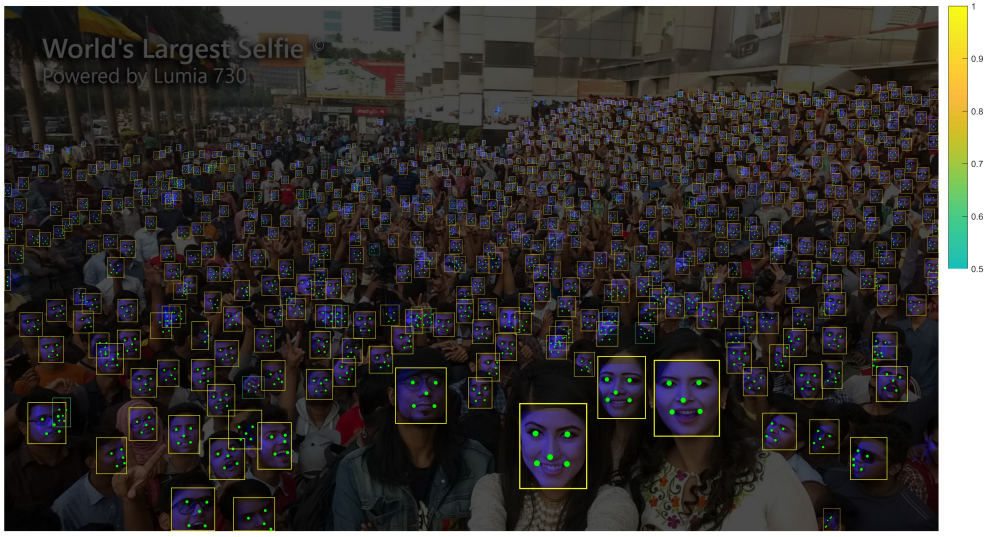
\includegraphics[width=0.85\textwidth]{figures/images/chapter-2/retinaface_example.png}
\caption{Qualitative example of face detection using RetinaFace in a crowded
real-world scene. Adapted from \cite{deng2020retinaface}.}
\label{fig:retinaface_example}
\end{figure}

RetinaFace also provides facial landmarks in addition to \gls{bounding box}es. The Figure~\ref{fig:retinaface_example} illustrates robust localization of many small and partially occluded faces. This supports downstream \gls{anonymization} steps where more precise localization is useful. RetinaFace was therefore selected as the face detector in \gls{SafeVision}.


\methodheading{PaddleOCR and Text Classification}

\gls{SafeVision} handles text-related \gls{anonymization} through a pipeline consisting of text detection, text recognition, and subsequent text classification. For text detection and recognition, the system uses PaddleOCR \cite{du2020ppocr}, which
provides an integrated \acrshort{ocr} framework for extracting textual content from natural images.

\begin{figure}[htbp]
\centering
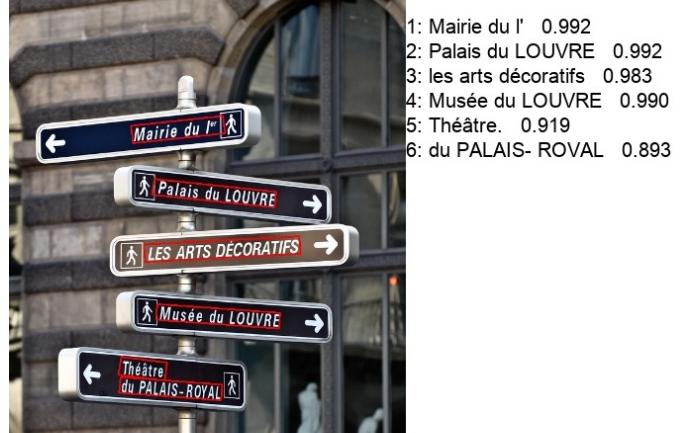
\includegraphics[width=0.70\textwidth]{figures/images/chapter-2/paddle_ocr_example.png}
\caption{Qualitative example of text detection and recognition using PaddleOCR
in a real-world scene. Adapted from \cite{du2020ppocr}.}
\label{fig:paddle_ocr_example}
\end{figure}

PaddleOCR was selected because it provides an end-to-end pipeline for localizing and recognizing text under varied visual conditions \cite{du2020ppocr}. This made it more suitable than generic \gls{object detection} alone, since text-based redaction depends on both identifying where text is located and extracting the content for further analysis.

After \acrshort{ocr}, the recognized text is further processed using a fine-tuned \acrshort{ner} model developed in this project, based on the XLM-RoBERTa base architecture \cite{conneau2020xlmroberta}. This was necessary 
because \acrshort{ocr} only extracts textual content, whereas selective redaction also  requires identifying which parts of the text belong to potentially sensitive entity categories. The combination of \acrshort{ocr} and \acrshort{ner}-based analysis therefore supports more selective and context-aware text redaction in \gls{SafeVision}.


\methodheading{\gls{yolox} for General and Custom Object Detection}

\Gls{object detection} in \gls{SafeVision} is based on \gls{yolox} \cite{ge2021yolox}. \gls{yolox} was selected because it combines strong detection performance with a simple and flexible framework for custom training. Its one-stage architecture makes it well suited for deployment and iterative experimentation.

\begin{figure}[H]
\centering
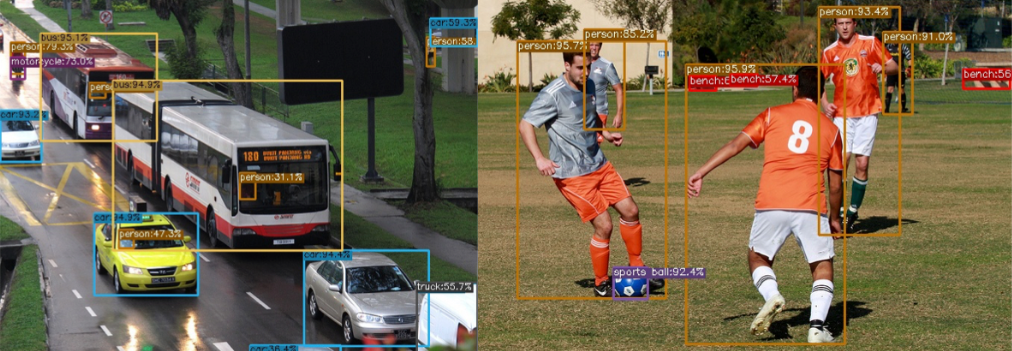
\includegraphics[width=\textwidth]{figures/images/chapter-2/yolox_example.png}
\caption{Qualitative example of \gls{object detection} using YOLOX. The figure illustrates localization of multiple object categories in natural scenes using \gls{bounding box}es and confidence scores. Adapted from \cite{yolox_github}.}
\label{fig:yolox_example}
\end{figure}

Within \gls{SafeVision}, \gls{yolox} is used in two different ways. First, existing \gls{yolox} models support detection of more general object categories relevant to the redaction workflow. Second, \gls{yolox} was used as the basis for custom-trained models targeting license plates and barcodes, where project-specific training was necessary. This made it possible to maintain a consistent detection framework while extending the system to object categories that were not sufficiently covered by the existing model setup.

The use of YOLOX also benefited from the availability of pretrained weights and well-documented training workflows in the official framework repository \cite{yolox_github,ge2021yolox}. This reduced training time and made it feasible to develop custom object detectors within the constraints of the project.


\methodheading{Video Processing and Tracking in \gls{SafeVision}}
\phantomsection
\label{sec:video_tracking_foundation}

\gls{SafeVision} handles video as a sequence of frames, where \gls{anonymization} must remain temporally consistent across time rather than being treated as a set of independent image outputs. For this reason, the system combines frame-level detection with tracking.

At user selected frames, \gls{SafeVision} applies the same detection pipeline used for still images. Between such frames, tracking is used to propagate and stabilize sensitive regions across consecutive frames, which reduces the need for repeated full detection and helps maintain visually consistent \gls{anonymization}.

For AI-generated detections, \gls{SafeVision} uses a multi-object tracking approach based on \gls{kalman filter}ing and entity specific association across frames \cite{bewley2016sort}. The tracker predicts \gls{bounding box}es over time and matches new detections to existing tracks using a combination of \gls{intersection over union} (\acrshort{iou}) and motion consistency. It also maintains track history and supports interpolation across detection gaps, which makes it
possible to backfill intermediate frames when detections are temporally sparse. 

For manually selected regions, \gls{SafeVision} uses a dedicated object-tracking component based on OpenCV tracking methods. The implementation prioritizes the ViT tracker from OpenCV Zoo when the required tracker implementation and ONNX model are available, because it provides a modern deep-learning-based tracking approach suitable for following user-defined objects across frames. Channel and Spatial Reliability Tracking (\acrshort{csrt}) is retained as a fallback because it is widely available in OpenCV and provides a practical conventional tracker when the ViT tracker cannot be used \cite{opencv_vittrack, lukezic2017csrt}. Manual tracking is applied forward and backward from the selected frame, allowing a user-defined \gls{bounding box} to be propagated through the surrounding sequence. Additional safety checks are used to detect unstable tracker output, including low confidence, implausible changes in size or aspect ratio, large center jumps, and weak overlap with the last trusted region.

\methodheading{\Gls{segmentation} and \Gls{inpainting} for Redaction Refinement}
\label{subsec:segmentation-and-inpainting-for-redaction-refinement}

To improve redaction quality beyond coarse \gls{bounding box} \gls{masking}, \gls{SafeVision} also includes refinement components for \gls{segmentation} and region replacement. For \gls{segmentation}, the system uses \gls{mobilesam} \cite{mobilesam}, a lightweight \gls{segmentation} model derived from the Segment Anything approach
\cite{kirillov2023segment}, in order to produce more precise masks for selected regions before redaction is applied.

\begin{figure}[H]
\centering
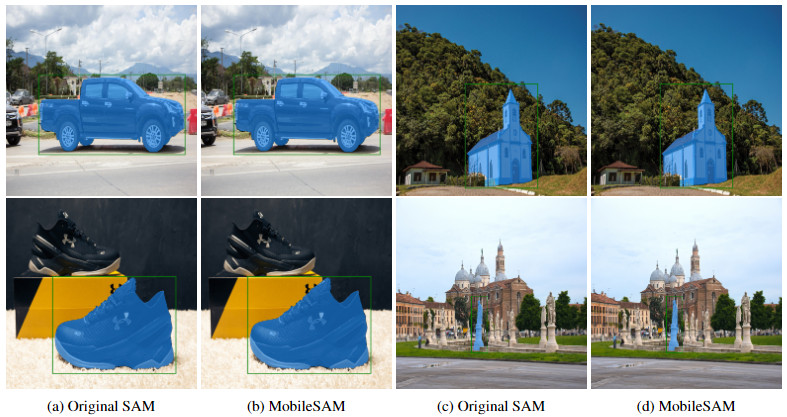
\includegraphics[width=0.8\textwidth]{figures/images/chapter-2/mobile_sam.png}
\caption{Comparison between \gls{segmentation} results produced by the original Segment Anything Model (\acrshort{sam})
and \gls{mobilesam}. The examples illustrate that \gls{mobilesam} can provide similar object masks while using a more lightweight model. Adapted from \cite{mobilesam}.}
\label{fig:mobile_sam}
\end{figure}

\gls{mobilesam} was selected to support more precise redaction where rectangular \gls{bounding box}es would include too much surrounding visual content. It enables more selective \gls{anonymization} than \gls{bounding box}-based redaction while remaining easier to integrate than heavier \gls{segmentation} models. Its compact size was also an important consideration, since \gls{SafeVision} is developed as a web application where lightweight and deployable components are preferable.

\begin{figure}[H]
\centering
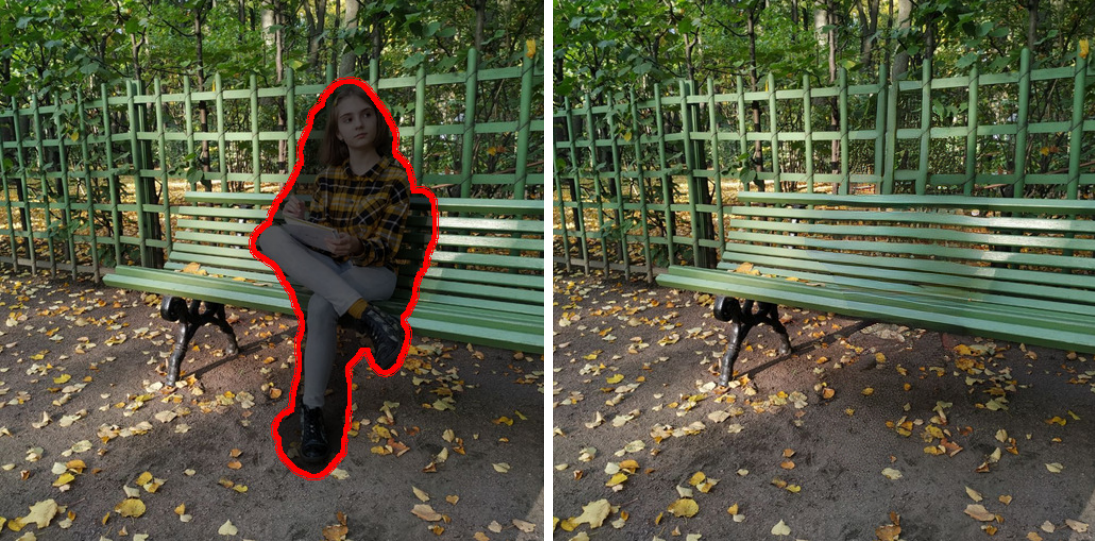
\includegraphics[width=0.7\textwidth]{figures/images/chapter-2/inpaint.png}
\caption{Illustration of image \gls{inpainting}, where a selected region is replaced
with generated background content instead of being masked directly. Adapted from
\cite{rombach2022high}.}
\label{fig:inpaint_example}
\end{figure}

For region replacement, the system uses a Stable Diffusion \gls{inpainting} model based on the \texttt{runwayml/stable-diffusion-inpainting} checkpoint \cite{sd_inpaint_model,rombach2022high}. This allows selected regions to be replaced with generated content instead of being blurred or masked directly. \Gls{inpainting} was nevertheless treated as a complementary refinement method rather than the default strategy, since visually cleaner output does not necessarily produce a more reliable form of \gls{anonymization}.


\methodheading{Why Hybrid User Review Was Retained}
\label{sec:why_hybrid_user_review_was_retained}

Although \gls{SafeVision} uses several strong AI-based components, the system was not designed as a fully autonomous redaction pipeline. Automated approaches still face practical limitations related to missed detections, \gls{false positive}s, and
context-dependent cases \cite{orekondy2017connecting, zhao2023visual}. User review was therefore retained as a central design principle in \gls{SafeVision}. Automatic detection reduces manual workload, while the user remains able to inspect, modify, and approve the final result before redaction is completed. This reduces reliance on fully automated decisions in cases where mistakes may expose sensitive information.

\section{Synthesis and Design Implications}

The reviewed theory and methods show that visual redaction requires a multi-component approach. Faces, embedded text, structured objects, and irregular regions differ in how they must be detected, interpreted, and anonymized. This motivated the use of specialized components in \gls{SafeVision}, rather than a single general-purpose model.

For video, this also introduces a temporal requirement: sensitive regions must be handled consistently across consecutive frames, which motivates the use of tracking mechanisms in addition to frame-level detection.

The review also shows that fully automated redaction remains limited by \gls{false negative}s, \gls{false positive}s, and context-dependent privacy risks. \gls{SafeVision} was therefore designed as a hybrid system: automated detection reduces manual work, while user review preserves control over the final anonymized output. These implications shaped the system requirements, architecture,
implementation, and evaluation presented in the following chapters.


\afterpage{\blankpage}

\chapter{Development Process}
\label{chap:devprocess}

This chapter describes how the project was carried out in practice. It presents the chosen development methodology of the project, the weekly work rhythm that was followed, the role of feedback, the main project phases, and the tools that were used in the development.

%------------------------- 3.1 -------------------------

\section{Group Background and Project Organization}
\label{sec:group-background-and-project-organization}

This bachelor thesis is carried out by three students enrolled in the Bachelor’s program in Data Engineering at the Norwegian University of Science and Technology (NTNU). Throughout the study program, the group members have acquired foundational knowledge in programming, software engineering, databases, and system architecture. The project allows this knowledge to be applied in a practical context while also emphasizing structured collaboration, version control, and agile working methodologies.

The project reflects the group’s technical interests while also providing practical experience with \acrshort{ml} and computer vision. The group’s motivation stems from a shared interest in these fields, which were among the most engaging topics in the study program. This project made it possible to work with training and fine-tuning \acrshort{ml} models, while also developing computer vision solutions related to privacy and security in visual media. Through experimentation, evaluation, and iterative refinement, theoretical concepts were applied to real-world challenges related to privacy and automated redaction. In this way, the work contributed to both academic development and practical competence building.

Responsibility was divided among the group members to structure the workload, including Scrum coordination, product responsibility, documentation, and development. Henrik Weflen Gjermundsen had responsibility as Scrum Master and backend developer, Karwan Shekhe had responsibility as product manager and backend developer, and An Hoang Chu had responsibility as documentation manager and frontend developer. These roles gave the group an initial structure which helped communication, meeting notes and product direction. All members contributed as developers, and tasks were redistributed as the project required support across frontend, backend, testing, research and report writing. The projectplan Appendix~\ref{appsec:group} further describes the formal role distribution and group routines in detail.




The project involved both collaboration with Safe Media AI and supervision from NTNU. SafeVision was developed with representatives from Safe Media AI, Jon Yngve Hardeberg and Yasin Hessnawi. The project was supervised by Tom Røise, a university lecturer at the Department of Information Technology and Informatics at NTNU in Gjøvik, who provided guidance on methodological choices, technical challenges, and the overall direction of the project.


%------------------------- 3.2 -------------------------



%------------------------- 2.3 -------------------------

\section{Development Methodology}
\label{sec:project-team-and-methodology}

The development process was based on the Scrumban methodology, which is also described in the project plan in Appendix~\ref{appsec:pfar}. Scrumban combines Scrum-based sprint structure with Kanban-based workflow visualization and task-flow management \cite{bhavsar2020scrumban}. This approach suited the project because the work involved technical uncertainty and changing priorities throughout the development period. The team needed to adjust continuously as available technologies were explored and new input was received from the project owners. A fixed plan would have been too rigid for this kind of project, while an unstructured process would have made coordination and progress tracking difficult.

Scrum was used to create a structured and adaptable development process. The work was organized into mostly one-week sprints, with some longer sprints later once the direction of the final project became clearer. This gave the group manageable planning periods in the early phases and made it possible to adapt when the work shifted from research and prototyping to integration and refinement. As outlined in the project plan in Appendix~\ref{appsec:pfar}, the sprint structure was supported by regular meetings, task distribution, and weekly logging, which made progress easier to track and helped keep the project aligned between the group members, the supervisor, and Safe Media AI.

\begin{figure}[H]
\centering
\resizebox{\textwidth}{!}{%
\begin{tikzpicture}[
    proc/.style={
        draw,
        rounded corners=2pt,
        fill=blue!10,
        align=center,
        minimum width=2.9cm,
        minimum height=1cm,
        font=\small
    },
    column/.style={
        draw,
        rounded corners=2pt,
        fill=gray!10,
        align=center,
        minimum width=2.1cm,
        minimum height=1cm,
        font=\small
    },
    ext/.style={
        draw,
        rounded corners=2pt,
        fill=green!10,
        align=center,
        minimum width=3.0cm,
        minimum height=0.9cm,
        font=\small
    },
    arrow/.style={-{Latex[length=2.2mm]}, thick},
    feedback/.style={-{Latex[length=2.2mm]}, thick, dashed}
]

% Feedback sources
\node[ext] (internal) at (1.4,4.2) {Internal team\\coordination};
\node[ext] (supervisor) at (5.0,4.2) {Supervisor\\feedback};
\node[ext] (commissioner) at (8.6,4.2) {Safe Media AI AS\\feedback};

% Sprint planning and backlog
\node[proc] (planning) at (1.4,2.1) {Sprint\\planning};
\node[proc] (backlog) at (5.0,2.1) {Sprint backlog\\and task selection};

% Kanban board background (moved slightly lower)
\draw[
    rounded corners=3pt,
    draw,
    fill=blue!4
] (6.8,-0.2) rectangle (19.1,2.4);

\node[font=\small\bfseries] at (12.95,1.95) {Jira / Kanban workflow};

% Kanban columns (moved lower)
\node[column] (todo) at (8.0,0.75) {To do};
\node[column] (progress) at (10.4,0.75) {In progress};
\node[column] (test) at (12.8,0.75) {To test};
\node[column] (review) at (15.2,0.75) {Review};
\node[column] (done) at (17.6,0.75) {Done};

% Main flow
\draw[arrow] (planning) -- (backlog);
\draw[arrow] (backlog) -- (todo);
\draw[arrow] (todo) -- (progress);
\draw[arrow] (progress) -- (test);
\draw[arrow] (test) -- (review);
\draw[arrow] (review) -- (done);

% Feedback arrows
\draw[feedback] (internal.south) -- (planning.north);
\draw[feedback] (supervisor.south) -- (backlog.north);
\draw[feedback] (commissioner.south) -- (backlog.north east);

\end{tikzpicture}%
}
\caption{Scrumban workflow used in the project, combining sprint-based planning with a Kanban task flow and feedback-based reprioritization.}
\label{fig:scrumban-workflow}
\end{figure}

Kanban contributed to flexible development by giving the team continuous visibility of the workflow. Tasks were created as issues through the Jira board and followed a flow where they moved from planning to active work, testing, review and completion. In this way, it became easier to reprioritize when new tasks appeared, when the group received feedback from the supervisor or Safe Media AI, or when obstacles came up during development. Kanban therefore supported a more adaptive process than a sprint plan alone could have provided.

\begin{figure}[H]
    \centering
    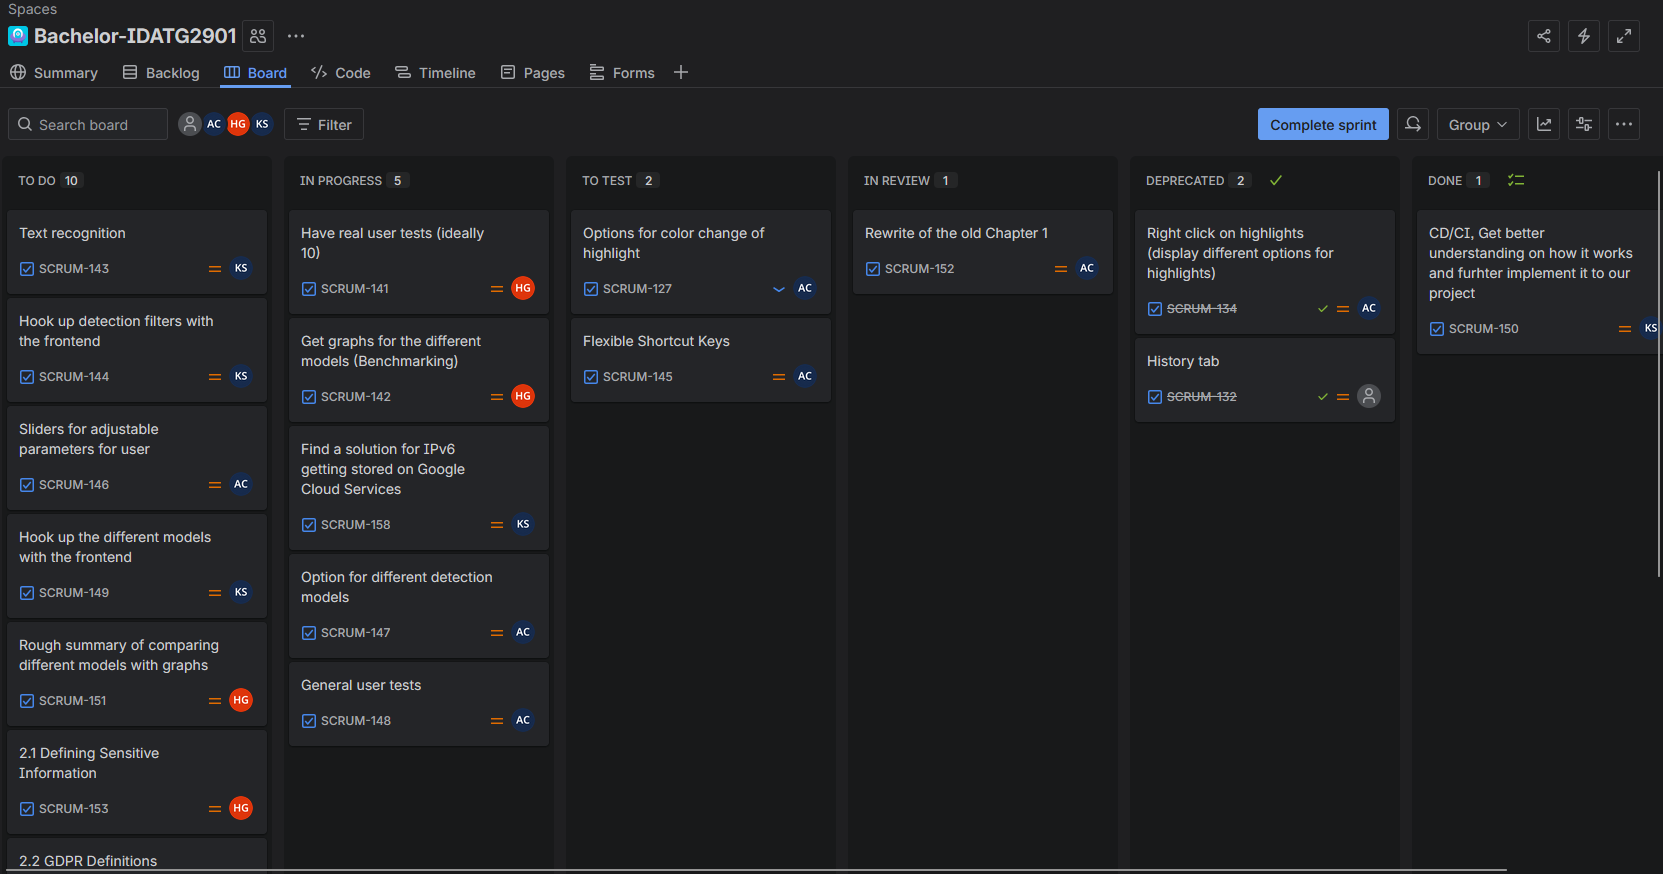
\includegraphics[width=\linewidth]{figures/images/chapter-4/jira_week9.jpg}
    \caption{Jira board snapshot from Week 9, showing active work related to feature development, testing and refinement.}
    \label{fig:jira-week9}
\end{figure}

In practice, the methodology was implemented through short sprint cycles, frequent internal coordination and regular reviews. Together, Scrum and Kanban provided a structured and adaptable development process (Figure~\ref{fig:scrumban-workflow}). This was important in a project where technical choices, feature priorities and implementation details had to be adjusted throughout. The use of Scrumban made it possible to maintain progress and direction, while still leaving room for change.


\section{Sprint Structure and Weekly Project Rhythm}

This section describes the weekly work rhythm and how it functioned in practice. It explains how the group worked in a structured and consistent way with sprint planning, daily coordination and regular review points. This rhythm followed the routines described in the project plan, where sprint planning, daily Scrum, sprint reviews and retrospectives were defined as part of the working method, see Appendix~\ref{app:project-plan}.

\methodheading{Sprint Planning and Task Management}

Each sprint began with sprint planning, where the group decided which tasks should be prioritized in the coming work. In the early stages of the project, this process was mainly used to discuss project planning, assignment clarification, administrative setup, and the distribution of research tasks. Later, when the direction of the project had become clearer, sprint planning was used to divide work related to implementation, integration, testing, refinement, and report writing. This gave the team a clear short-term direction and made the project easier to manage step by step. Tasks were assessed through group discussion based on expected complexity, uncertainty, and available capacity. Larger tasks were divided into smaller issues when they became too broad to assign or complete within a sprint.

Tasks created in sprint planning were tracked as issues on the project’s issue board, where they were assigned to group members corresponding to the planning, Figure~\ref{fig:jira-week9}. This made it easier to divide larger goals discussed into smaller work tasks which could coexist with other new findings or technical challenges. Sprint planning therefore functioned both as coordination and as a way of keeping the tasks manageable. The planned sprint rhythm and meeting structure were defined in the project plan, including sprint planning, daily Scrum, sprint reviews and retrospectives, see Appendix~\ref{app:project-plan}.

\methodheading{Daily Coordination and Follow-Up}

Daily Scrum was used to maintain alignment within the group between sprint planning and weekly review meetings. The group contract in Appendix~\ref{app:project-plan} describes the routines established for frequent internal follow-up meetings throughout the week. These meetings were used to clarify completed work, ongoing tasks, and any blockers that needed to be addressed before the next milestone.

This continuous coordination was especially useful in a project where technical choices, implementation details and scope questions developed over time. In addition to daily Scrum, the group also worked together physically and digitally to solve problems and prepare for meetings. The daily coordination therefore helped maintain momentum in the project and the development process coherent.

\methodheading{Sprint Reviews and Retrospectives}

Sprint reviews and retrospectives were closely tied to the meeting with the supervisor and Safe Media AI. These meetings worked as natural review points for the group where status was presented, feedback was received, and afterwards a discussion of how the project can move forward. Input from these weekly sessions was often used directly to adjust scope, clarify technical direction and decide what should be prioritized in the coming sprint.

This structure gave the team a continuous opportunity to reflect on the product and the process. What had worked well, what had created problems and what was the strategy going to be in the coming phase. In this way, the review structure also supported continuous improvement throughout the project. The sprint reviews did not only mark the end of one work period, but they became an important mechanism for learning and helped connect weekly development to broader academic and practical expectations.

%------------------------- 3.4 -------------------------

\section{Stakeholder Involvement}
\label{sec:stakeholder-involvement-external-feedback}

Throughout the project, feedback from both the supervisor and Safe Media AI helped shape the direction, scope, and priorities of the work. Selected meetings that influenced the development process are summarized in Table~\ref{tab:meeting-impact}, while the full selected meeting notes are included in Appendix~\ref{app:meeting-notes}. The feedback was important not only for deciding which features to develop, but also for determining which ideas should remain outside the final scope. This helped the group prioritize relevant tasks, avoid unnecessary expansion of the system, and connect the technical development to both practical needs and academic expectations.

\begingroup
\scriptsize
\setlength{\tabcolsep}{3pt}
\renewcommand{\arraystretch}{1.08}
\setlength{\LTpre}{0.4em}
\setlength{\LTpost}{0.4em}

\begin{xltabular}{\textwidth}{
    >{\raggedright\arraybackslash}p{2.7cm}
    >{\raggedright\arraybackslash}X
}
\caption{Condensed overview of selected project meetings and their influence on project decisions.}
\label{tab:meeting-impact}\\

\toprule
\textbf{Date and type} & \textbf{Main outcome and project impact} \\
\midrule
\endfirsthead

\toprule
\textbf{Date and type} & \textbf{Main outcome and project impact} \\
\midrule
\endhead

\midrule
\multicolumn{2}{r}{\footnotesize Continued on next page} \\
\endfoot

\bottomrule
\endlastfoot

\meetingcell{08.01.2026}{Internal group meeting}{app:meeting-2026-01-08}
& Established the initial project structure, including administrative setup, role distribution, Scrum routines, work logging, GitLab issues, Overleaf documentation and the need for a group contract. \\

\meetingcell{09.01.2026}{Internal group meeting}{app:meeting-2026-01-09}
& The group decided to pursue the Safe Media AI AS assignment as the preferred project direction, contacted the commissioner and prioritized completing enough of the project plan to receive early supervisor feedback. \\

\meetingcell{15.01.2026}{Startup meeting with commissioner}{app:meeting-2026-01-15}
& Clarified the assignment direction with Safe Media AI AS. Image redaction became the main starting point, React or Vue was recommended for the frontend, Python for the backend, and faces and text were identified as early detection priorities. \\

\meetingcell{22.01.2026}{Commissioner meeting}{app:meeting-2026-01-22}
& Defined the integration boundary more clearly. The group should limit the core system to image-based redaction, while Safe Media AI AS' existing system could handle document-level PDF workflows. Manual user correction was emphasized as a core requirement. \\

\meetingcell{26.01.2026}{Supervisor meeting}{app:meeting-2026-01-26}
& Received feedback on the project plan and report direction. The supervisor emphasized academic justification of technical choices and recommended using an early throwaway prototype to explore tools before committing to the real MVP. \\

\meetingcell{29.01.2026}{Commissioner meeting}{app:meeting-2026-01-29}
& Presented early prototype progress and agreed on closer weekly commissioner involvement. The meeting influenced later work on redaction strength, privacy, user trust, possible video tracking and research into \acrshort{gdpr} and \gls{anonymization} practice. \\

\meetingcell{09.02.2026}{Supervisor meeting}{app:meeting-2026-02-09}
& Clarified the evaluation priorities. The supervisor emphasized testing both correct and incorrect detections, documenting model quality with evidence, checking model licensing and considering privacy risks related to image and video processing. \\

\meetingcell{12.02.2026}{Commissioner meeting}{app:meeting-2026-02-12}
& Confirmed that full PDF handling should remain outside the core backend because Safe Media AI AS already handled PDF extraction. The meeting reinforced image-based processing, \acrshort{ocr}/text detection, performance expectations, private repositories and early deployment planning. \\

\meetingcell{16.02.2026}{Supervisor meeting}{app:meeting-2026-02-16}
& Supported moving PDF handling into project limitations and defining image redaction as the main subject of the report. The supervisor encouraged deeper technical evaluation of speed, privacy, model quality, parallel detection and relevant scientific literature. \\

\meetingcell{19.02.2026}{Commissioner meeting}{app:meeting-2026-02-19}
& Influenced feature priorities for the MVP, including file-format support, improved text detection, filter options, manual marking, adjustable highlight boxes, response structure, benchmarking, user testing and possible ground-truth data collection. \\

\meetingcell{05.03.2026}{Commissioner meeting}{app:meeting-2026-03-05}
& Explored video, advanced options and practical user needs. Video was considered relevant but secondary, while expert-mode options, interface complexity and real-world redaction workflows were identified as important design considerations. \\

\meetingcell{09.03.2026}{Supervisor meeting}{app:meeting-2026-03-09}
& Refined the user-test plan. The supervisor advised that the test should support evaluation rather than sales, assess the basic image workflow, use clear tasks and images, and treat video mainly as a proof of concept or future direction. \\

\meetingcell{18.03.2026}{Commissioner meeting}{app:meeting-2026-03-18}
& Clarified Application Programming Interface (\acrshort{api}) based integration with Safe Media AI AS and the need to consider memory use, processing time and computational requirements. The meeting also narrowed video-related goals and emphasized feasible scope control. \\

\meetingcell{23.03.2026}{Supervisor meeting}{app:meeting-2026-03-23}
& Helped control the project scope after many explored directions, including JPEG, PNG, PDF, video, metadata and surveys. The supervisor advised defining detection and redaction as the main content of the report, with less central experiments moved to appendices. \\

\meetingcell{13.04.2026}{Supervisor meeting}{app:meeting-2026-04-13}
& Provided report feedback for the remaining project period. The supervisor emphasized improving the abstract and summary, connecting theory more directly to the project, strengthening GDPR and sensitive-information discussion, and explaining development-process choices rather than only listing chronology. \\

\meetingcell{22.04.2026}{Guidance for user testing and UI design}{app:meeting-2026-04-22}
& Provided feedback on user communication during processing, video settings, report framing, benchmarking and interface terminology. The meeting also clarified that \gls{inpainting} should be presented as part of the explored and implemented functionality if the achieved results were usable. \\

\meetingcell{23.04.2026}{Supervisor meeting}{app:meeting-2026-04-23}
& Set the final phase priorities as report quality, testing, figures and security. The supervisor recommended improving readability, clearly discussing figures, showing implementation progress, documenting implemented security measures and avoiding unnecessary new functionality near the deadline. \\

\end{xltabular}

\vspace{0.3em}
\noindent\footnotesize\textit{Note.} This table presents a summary of selected meeting notes. The meeting content was summarized with artificial intelligence and reviewed by the project group.

\endgroup

The supervisor contributed mainly through guidance on group structure, prioritization, documentation, and report writing. This became especially important after the group had developed a working version of the system and began considering possible extensions. Through these discussions, the group was encouraged to document added functionality properly rather than trying to include every explored idea in the final product. Several meetings were also used to review report chapters and clarify what belonged in the main thesis.

Safe Media AI contributed mainly to the practical and product-oriented direction of the project. Their feedback helped clarify the project scope, feature priorities, integration boundaries, and expectations for the delivered prototype. This ensured that the development process was connected to practical needs rather than only the group’s own assumptions. 


\section{Project Timeline and Milestone Development}
\label{sec:project-timeline-milestones}

Figure~\ref{fig:project-timeline} summarizes the main phases of the project from January to May. The timeline is divided into five phases, showing how the work developed from assignment clarification and early exploration to implementation, user feedback, scope narrowing, and final documentation.

\begin{figure}[H]
\centering
\resizebox{\textwidth}{!}{%
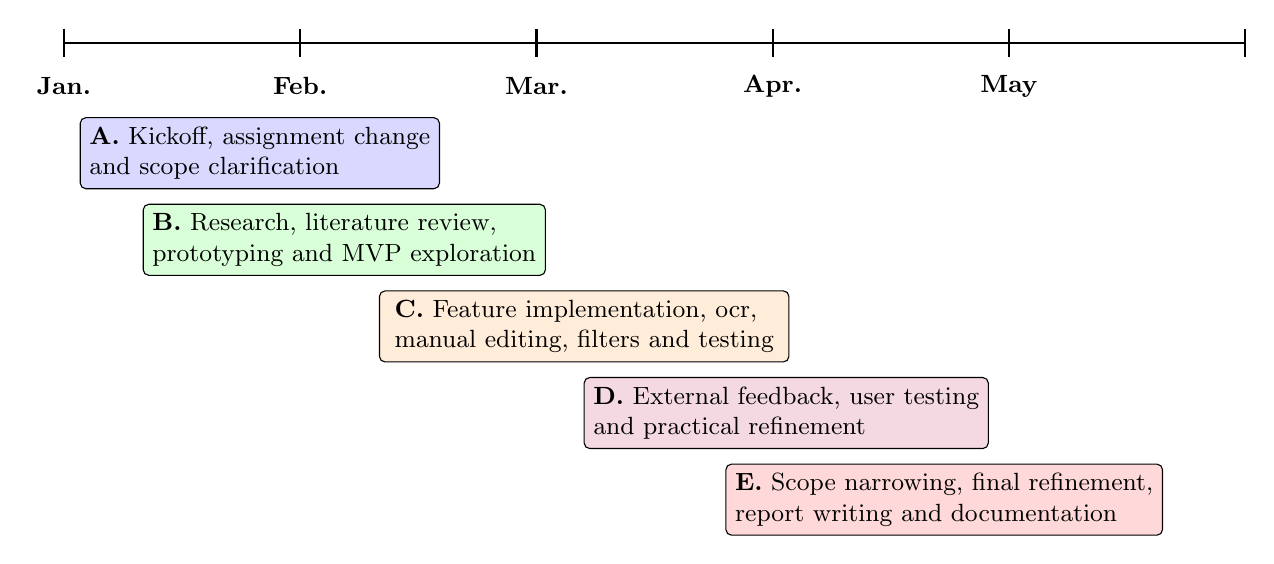
\begin{tikzpicture}[
    phase/.style={
        draw,
        rounded corners=2pt,
        align=left,
        minimum height=0.9cm,
        font=\small
    }
]

% Main timeline
\draw[thick] (0,0) -- (15,0);

% Month ticks and labels
\foreach \x/\m in {0/Jan.,3/Feb.,6/Mar.,9/Apr.,12/May}
{
    \draw[thick] (\x,0.18) -- (\x,-0.18);
    \node[font=\small\bfseries] at (\x,-0.55) {\m};
}
\draw[thick] (15,0.18) -- (15,-0.18);

% Phase boxes below the timeline
\node[phase, fill=blue!15, anchor=west, minimum width=3.2cm] at (0.2,-1.4)
{\textbf{A.} Kickoff, assignment change\\and scope clarification};

\node[phase, fill=green!15, anchor=west, minimum width=4.8cm] at (1.0,-2.5)
{\textbf{B.} Research, literature review,\\prototyping and MVP exploration};

\node[phase, fill=orange!15, anchor=west, minimum width=5.2cm] at (4.0,-3.6)
{\textbf{C.} Feature implementation, \acrshort{ocr},\\manual editing, filters and testing};

\node[phase, fill=purple!15, anchor=west, minimum width=4.5cm] at (6.6,-4.7)
{\textbf{D.} External feedback, user testing\\and practical refinement};

\node[phase, fill=red!15, anchor=west, minimum width=5.2cm] at (8.4,-5.8)
{\textbf{E.} Scope narrowing, final refinement,\\report writing and documentation};

\end{tikzpicture}%
}
\caption{Project timeline showing the main phases from assignment clarification to final refinement and documentation.}
\label{fig:project-timeline}
\end{figure}

The first phase consisted of kickoff, assignment change, and scope clarification. The project began with a transition period involving a change in assignment, role organization, and initial planning with the supervisor. During the first weeks, the group briefly collaborated with a different external client, but the cooperation was discontinued at an early stage. After securing the new assignment with Safe Media AI, the group prioritized scope clarification and early research. The team discussed what the solution should address, how sensitive information should be understood in visual media, and which technical and practical boundaries needed to be defined from the start. This transition is documented in the project plan in Appendix~\ref{app:project-plan}.

The second phase focused on research, literature review, prototyping, and MVP exploration. During this stage, the group investigated relevant models, datasets, and technical approaches that could support the final solution. Early frontend and backend prototypes were tested to explore possible implementation directions. The goal of this phase was to identify a workable technical foundation and establish an MVP that could guide further development.

The third phase centered on feature implementation and technical expansion. After the MVP had established a more stable foundation, the work shifted from exploration to building functionality on top of the existing system. This included image-based detection and redaction, \acrshort{ocr} and text processing, manual editing of \gls{bounding box}es, filtering options, redaction modes, deployment work, and testing. During this phase, the system evolved from an early prototype into a more complete and usable application.

The fourth phase emphasized external feedback and user testing. A meeting with Skan-Kontroll gave the group insight into how redaction could be relevant in practical workflows, while UX guidance from Thomas Berg Fjellestad contributed feedback on interface clarity and workflow design. Together with the group’s own testing, this phase helped evaluate usability and practical relevance. The structured user testing itself is discussed separately in Section~\ref{sec:user-testing}.

The final phase consisted of scope narrowing, final refinement, report writing, and documentation. Several possible directions had been explored during development, including video support, benchmarking, QR and barcode detection, metadata-related handling, and interface refinement. At this stage, the group prioritized the most achievable and relevant deliverables, with the image based workflow remaining the core functionality of the system.

\section{Tools and Working Practices}
\label{sec:tools-and-working-practices}

The project was supported by a set of tools for communication, planning, documentation, and practical collaboration. These tools helped structure the development process and supported both the technical work and the written thesis. Rather than being part of the system itself, they were used to coordinate tasks, document progress, and support the group’s daily workflow.

\begin{table}[H]
\centering
\caption{Main tools used to support project work}
\label{tab:project_tools}
\begin{tabular}{p{3.2cm} p{10.2cm}}
\toprule
\textbf{Tool} & \textbf{Purpose in the project} \\
\midrule
Jira & Planning, task distribution, and issue tracking \\

GitHub & Version control and collaborative code management \\

Figma & Creation of low-fidelity wireframes for early interface design \\

Excel & Hour logging and short weekly summaries of completed work \\

Discord & Internal communication within the group \\

draw.io & Creation of diagrams and figures \\

LaTeX / Overleaf & Thesis writing and report formatting \\

Word & Supporting documentation and meeting material \\

VS Code & Shared development environment for implementation work \\
\bottomrule
\end{tabular}
\end{table}

Jira was used for planning and issue tracking, which supported the Scrumban-based work process. GitHub was used for version control and collaborative code management, while VS Code was the shared development environment used by the group. Discord and physical meetings were used for internal communication, and Teams was used in several meetings with Safe Media AI AS.

\begin{figure}[H]
    \centering
    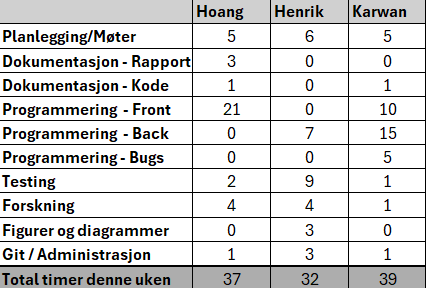
\includegraphics[width=0.95\textwidth]{figures/images/chapter-3/timeliste.png}
    \caption{Example from the project hour list, showing work distribution during week 9.}
    \label{fig:project_hour_list_example}
\end{figure}

Documentation and reporting were supported through LaTeX in Overleaf, together with Word and Excel (Figure~\ref{fig:project_hour_list_example}) for supplementary project material such as meeting notes and hour logging, further detailed spreadsheet for the hour list is in Appendix~\ref{app:project-hour-tracking}. In addition, Figma was used to sketch low-fidelity wireframes, and draw.io was used to create diagrams and figures. A summary of the main tools used in the project is provided in Table~\ref{tab:project_tools}.

\begin{figure}[H]
    \centering
    \makebox[\textwidth][c]{%
        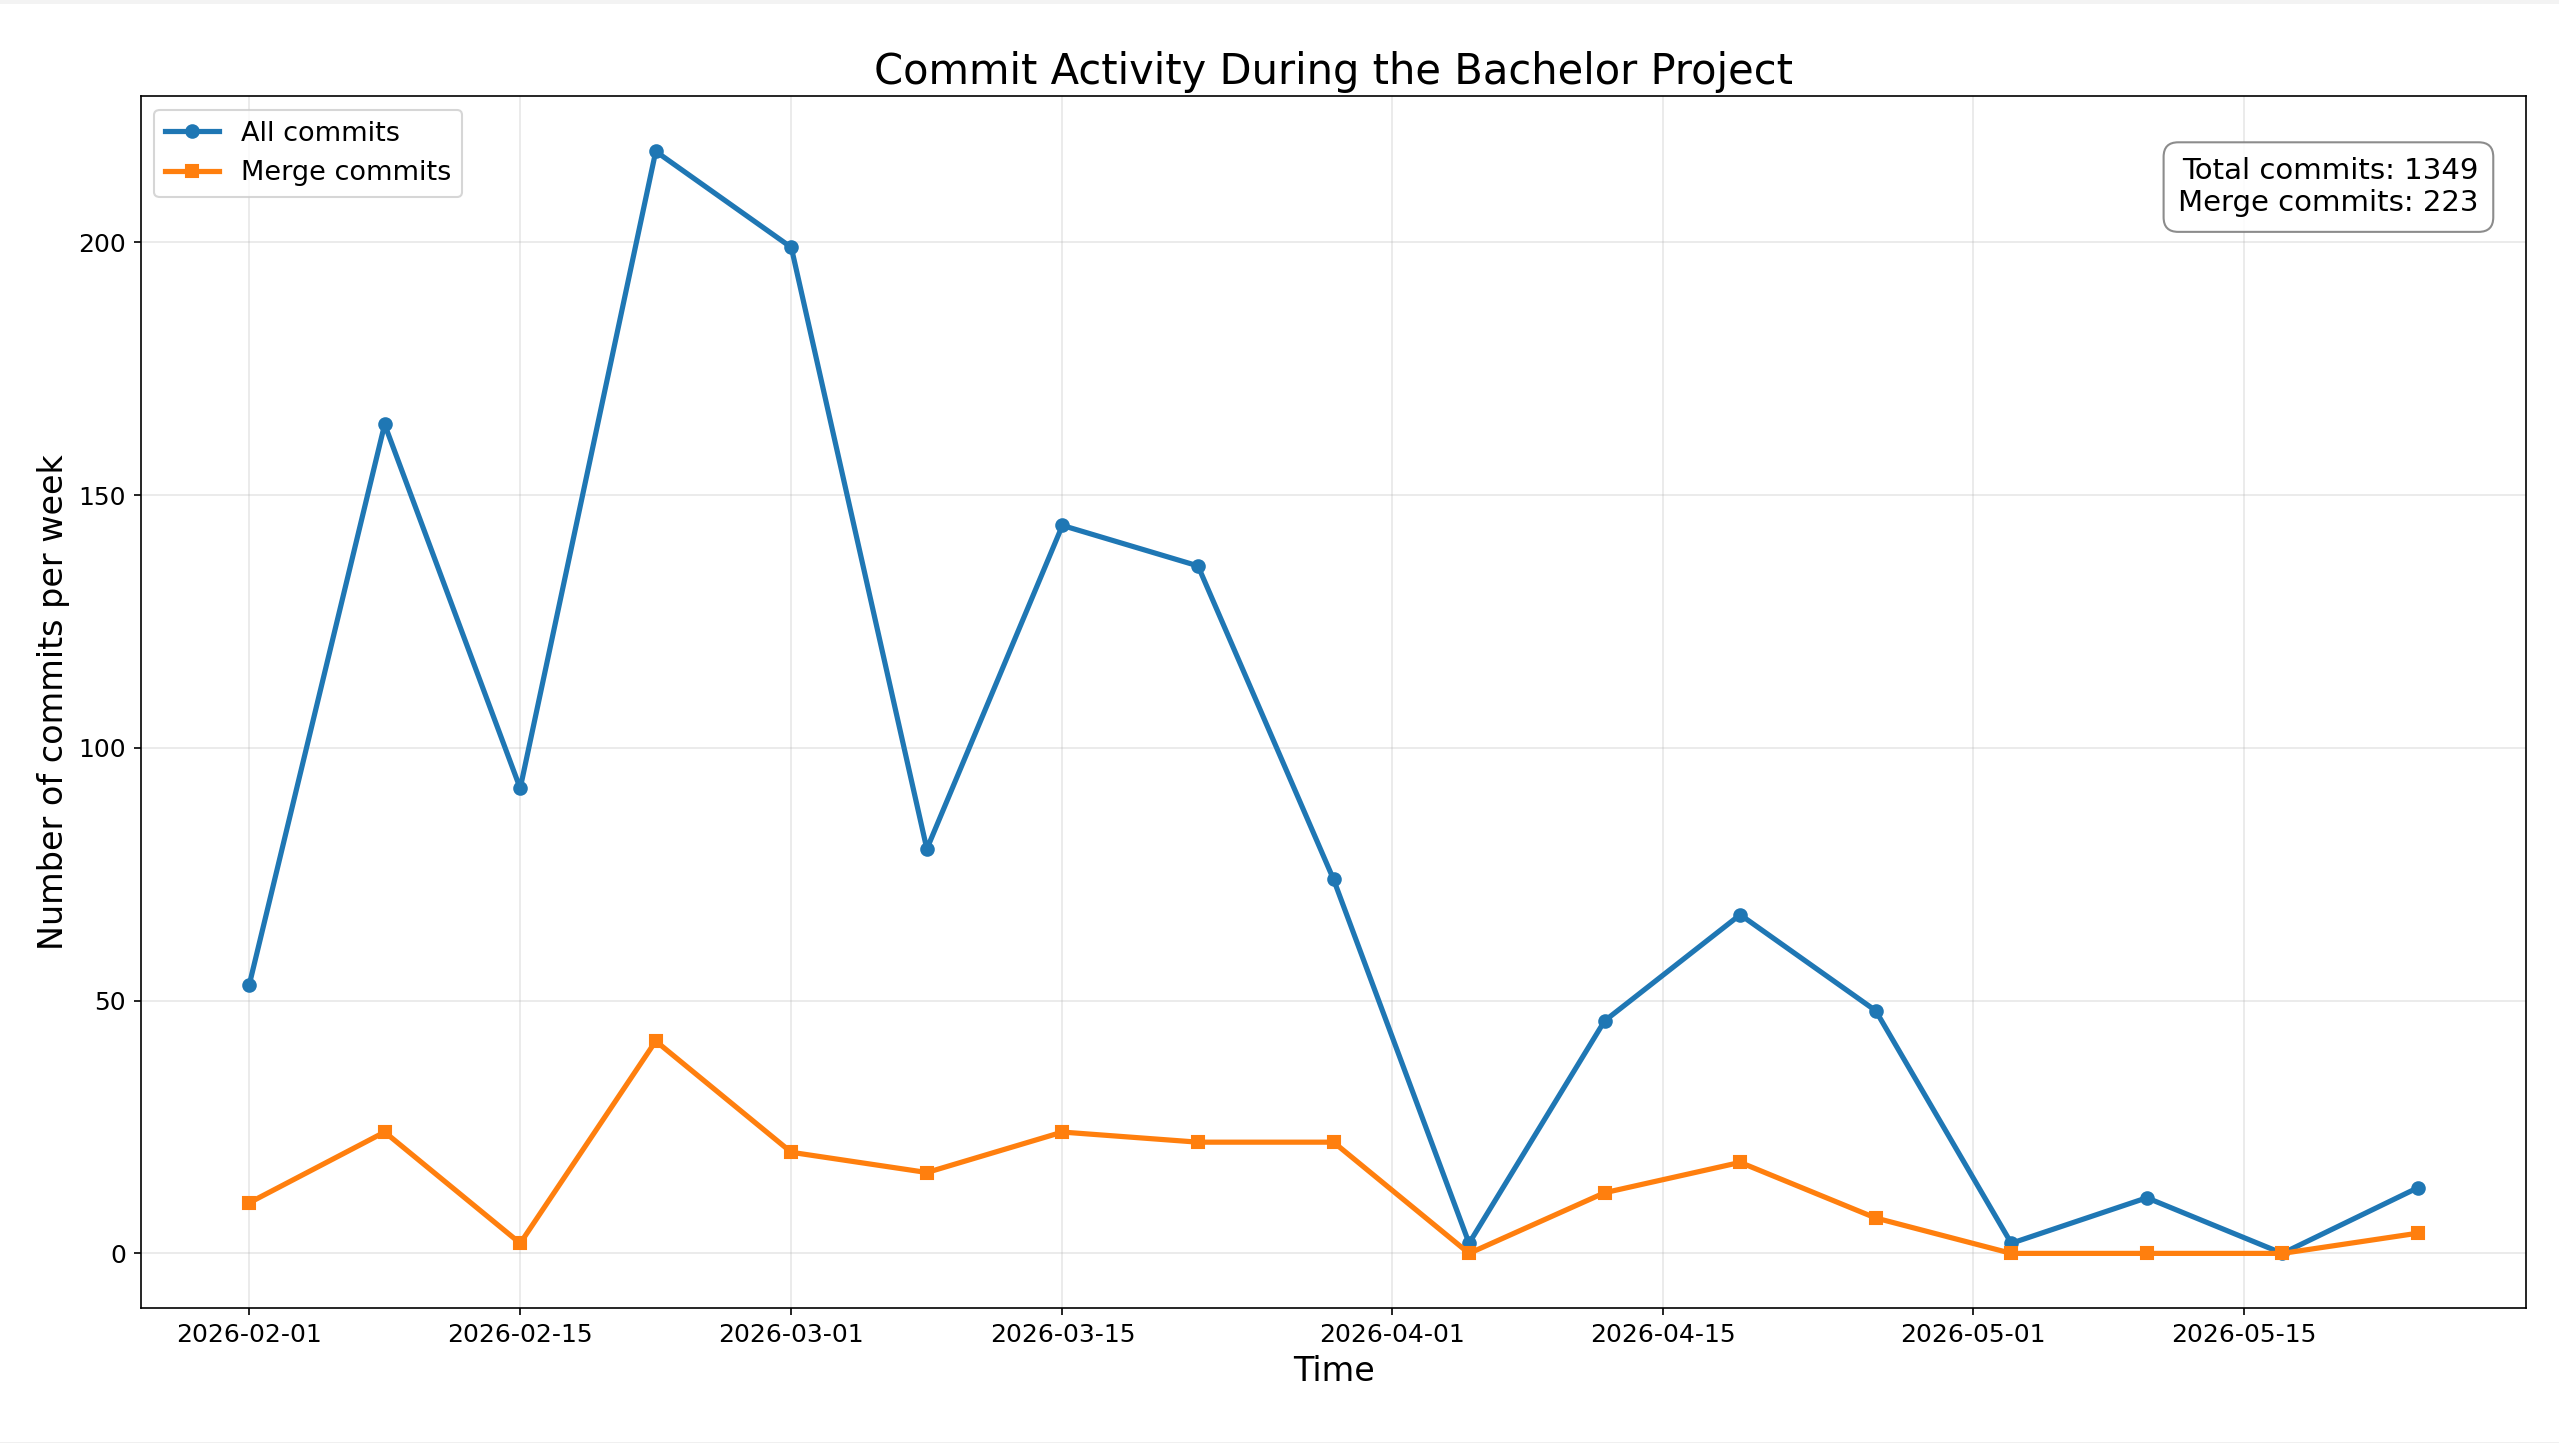
\includegraphics[width=1.3\linewidth]{figures/images/chapter-3/commit_merge_timeline.png}%
    }
    \caption{GitHub commit activity during the project period, showing how implementation work was distributed over time.}
    \label{fig:github_commit_timeline}
\end{figure}

The GitHub commit history provides an overview of the actual implementation activity during the project. Figure~\ref{fig:github_commit_timeline} shows how development work was distributed over time, including periods of higher implementation intensity and later refinement. The timeline supports the project history described in this chapter by showing that development was carried out continuously rather than being concentrated only near the end of the project.

\section{Artificial Intelligence as a Development Tool}
\label{sec:ai-development-tool}

Artificial intelligence was used as a supporting tool throughout the project, but not as an independent decision maker. Its role was to provide suggestions, help clarify problems, and reduce time spent on repetitive or clearly defined tasks. All outputs that affected the system, report, or technical decisions were reviewed, tested, and adapted by the group before being included.

In development work, the support mainly involved code review, error explanation, alternative implementation suggestions, and smaller debugging tasks. Generated code was not copied directly into the system without evaluation since the suggestions often had to be adjusted to fit the existing architecture and implementation choices. The tools also contributed to code documentation by helping formulate explanations of selected implementation details.

For technical research and problem solving, AI helped compare possible approaches and identify relevant technologies or methods. This was useful when the group needed an initial overview of different implementation alternatives before evaluating them more critically. In the \acrshort{ml} part of the project, synthetic text examples were generated for the text classification pipeline, including examples of sensitive and non-sensitive text entities. These examples were treated as supporting material and reviewed before use.

In the report work, AI contributed to spelling correction, sentence reformulation, clarification of technical explanations, and troubleshooting of LaTeX or Overleaf compiler errors. The final wording, technical content, and project decisions remained the responsibility of the group, and the suggestions were adjusted to match the actual implementation and writing style of the thesis.


\chapter{Software Requirements Specification}
\label{chap:software_requirements_specification}

This chapter defines the requirements that guided the design and development of \gls{SafeVision}. It presents the main functional requirements, describes central use cases for detection and redaction, and outlines the non-functional requirements related to security, performance, usability, and maintainability. The chapter also explains how the requirements were prioritized to support a practical development process and ensure that the most important functionality was implemented first.

%------------------------- 4.1 ---------------------------

\section{Functional Requirements}

Functional requirements describe the core capabilities that the system must provide. These requirements are derived from the problem statement and scope in Section~\ref{sec:problem-statement-and-scope}, the project delimitations in Section~\ref{sec:delimitation}, and the stakeholder meetings summarized in Table~\ref{tab:meeting-impact}. The requirements therefore reflect both the original project direction and the practical feedback received from Safe Media AI and the supervisor during development.

\begin{table}[H]
\centering
\begin{tabular}{|p{5cm}|p{9cm}|}
\hline
\textbf{Requirement} & \textbf{Description} \\ \hline

\textbf{Automatic Detection of Sensitive Information} & 
The system shall automatically detect sensitive information in images, including faces and textual content. \\ \hline

\textbf{Image File Support} & 
The system shall support commonly used image formats such as PNG and JPEG. \\ \hline

\textbf{Manual Editing of Detection Results} & 
The system shall allow users to review, modify, and remove detected regions before redaction is applied. \\ \hline

\textbf{Multiple Redaction Methods} & 
The system shall support different redaction techniques such as blurring, pixelation, and \gls{masking}. \\ \hline

\textbf{Redaction Execution} & 
The system shall apply selected redaction methods to user-defined or detected regions. \\ \hline

\textbf{Process Speed} &
The detection process should not be noticeably longer than Safe Media AI's detection system. \\ \hline

\textbf{System Integration Capability} & 
The system should be designed in a way that allows integration with external systems through well-defined interfaces. \\ \hline

\end{tabular}
\caption{Functional Requirements for the \gls{SafeVision} System}
\label{tab:functional_requirements}
\end{table}

%------------------------- 4.2 ---------------------------

\section{Use Case Details}

Use cases further illustrate how users interact with \gls{SafeVision} to achieve the main goals of the system. Whereas the functional requirements define the capabilities the system must provide, the use cases show how these capabilities are combined in practice. For \gls{SafeVision}, this is especially important because the workflow combines automated detection with user review, allowing the system to support the user while leaving the final redaction decisions under user control.

Figure~\ref{fig:safevision_usecase} presents a high-level overview of the system's use cases. The main workflow consists of uploading visual media, detecting sensitive information, reviewing the detected regions, adjusting the results when necessary, applying redaction, and verifying the processed output. These interactions form the basis for the sequence diagrams below, which describe the two most central workflows in more detail.

\begin{figure}[H]
\centering
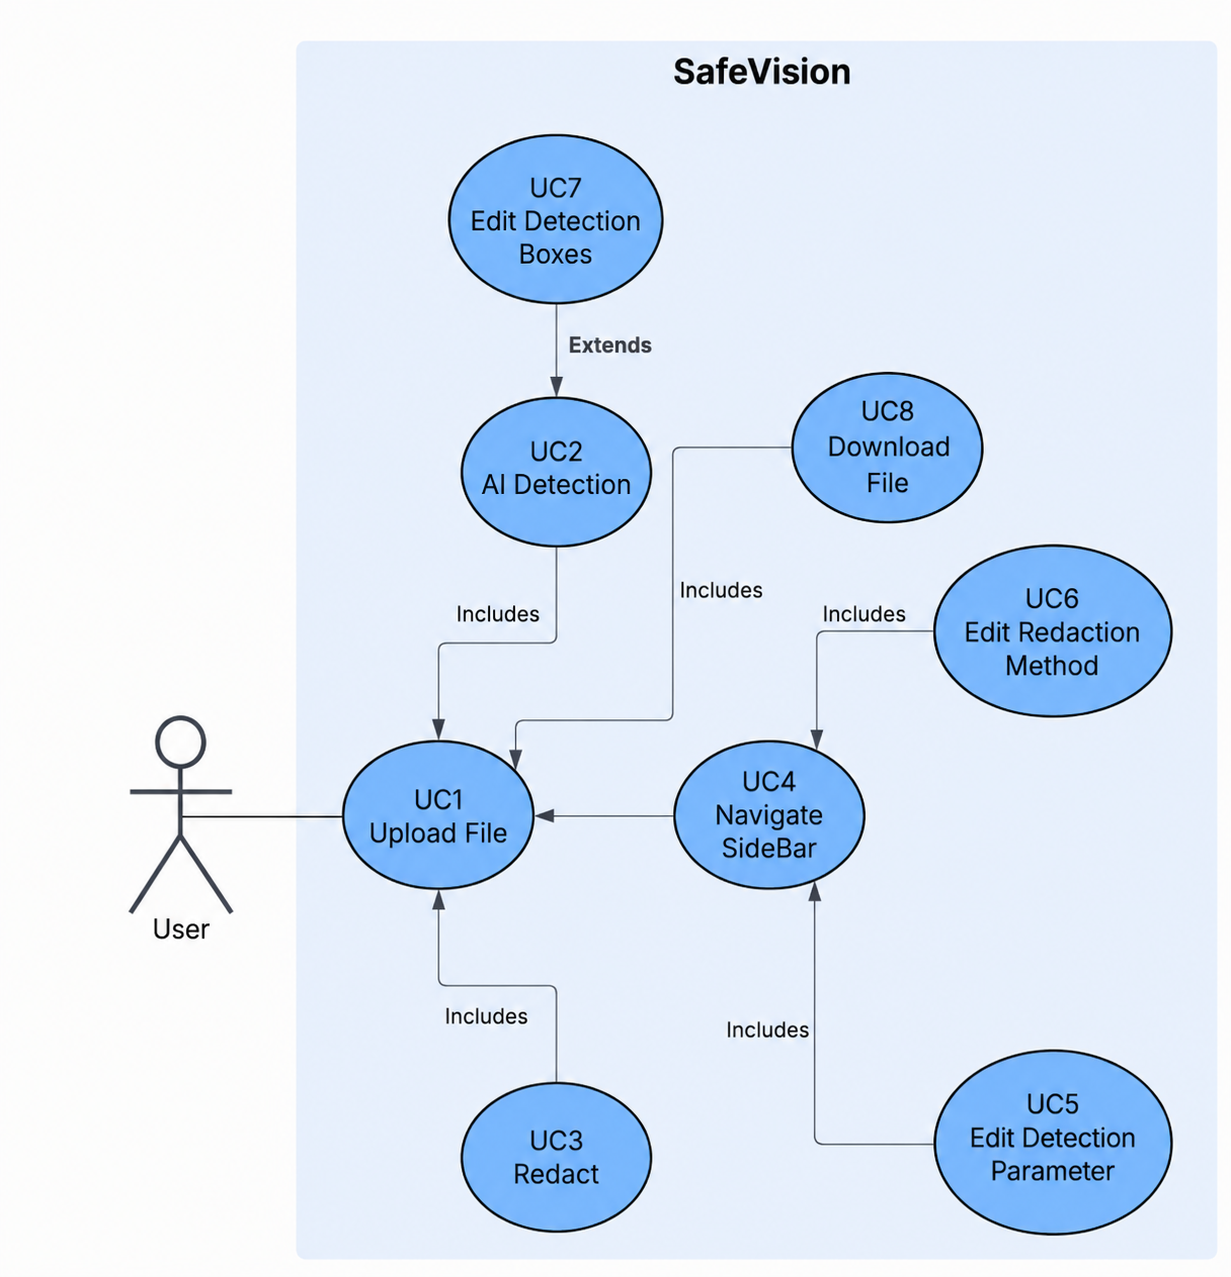
\includegraphics[width=0.8\textwidth]{figures/images/chapter-3/SafeVisionUseCase.png}
\caption{Use case diagram for the \gls{SafeVision} system}
\label{fig:safevision_usecase}
\end{figure}

\methodheading{Image Detection Scenario}

-As shown in Figure~\ref{fig:sequence_detection}, the image detection scenario begins when the user uploads an image through the interface and starts the detection process. \gls{SafeVision} then sends the image to the backend, where the relevant detection components analyze it and identify regions that may contain sensitive information. Once the analysis is complete, the detected regions are returned to the frontend and displayed as editable areas. Rather than being treated as final decisions, these results function as suggestions that the user can review, adjust, remove, or supplement with manually added regions before continuing. In this way, the workflow keeps the user in control of the detection outcome and reduces the risk of relying blindly on automated results.

\begin{figure}[H]
    \centering
    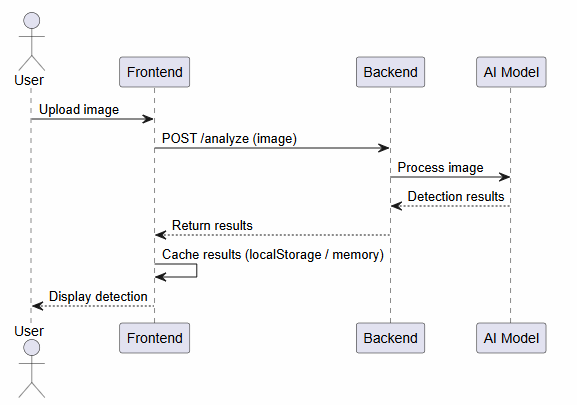
\includegraphics[width=0.9\textwidth]{figures/images/chapter-3/SequenceDetection.png}
    \caption{Sequence diagram illustrating the image detection interaction}
    \label{fig:sequence_detection}
\end{figure}

\methodheading{Redaction Scenario}

The redaction scenario follows the same overall interaction structure as the detection scenario shown in Figure~\ref{fig:sequence_detection}, but begins after the user has reviewed the detected regions. At this stage, the user decides which areas should be anonymized and selects an appropriate redaction method, such as blur, pixelation, or \gls{masking}. For standard redaction methods, the selected regions and settings are processed directly by the backend before the updated result is returned to the frontend. If the user instead selects \gls{segmentation} or \gls{inpainting}, the request is passed to the relevant AI-based processing components before the final result is generated. In both cases, the redacted output is presented to the user for verification before further use. This means that successful \gls{anonymization} depends not only on detecting relevant regions, but also on whether the final output sufficiently hides sensitive information.

Combined, these scenarios demonstrate how \gls{SafeVision} connects automated processing with user-guided verification. Detection and redaction are supported as linked workflow steps, while users can inspect and correct results before final \gls{anonymization}. As a result, the system supports both usability and reliability when handling sensitive information in visual media.

%------------------------- 4.3 ---------------------------

\section{Non-Functional Requirements}
\label{sec:nfr}

Beyond the core functional capabilities of detecting and redacting sensitive information, \gls{SafeVision} must satisfy several non-functional requirements that define the overall quality attributes of the system. These requirements guide architectural and implementation decisions by describing how the system should behave, rather than only what it should do. In this project, the non-functional requirements are categorized into four main areas: \textit{security}, \textit{performance}, \textit{usability}, and \textit{maintainability}, as illustrated in Figure~\ref{fig:non_functional_req}.

\begin{figure}[H]
    \centering
    \resizebox{0.92\textwidth}{!}{%
    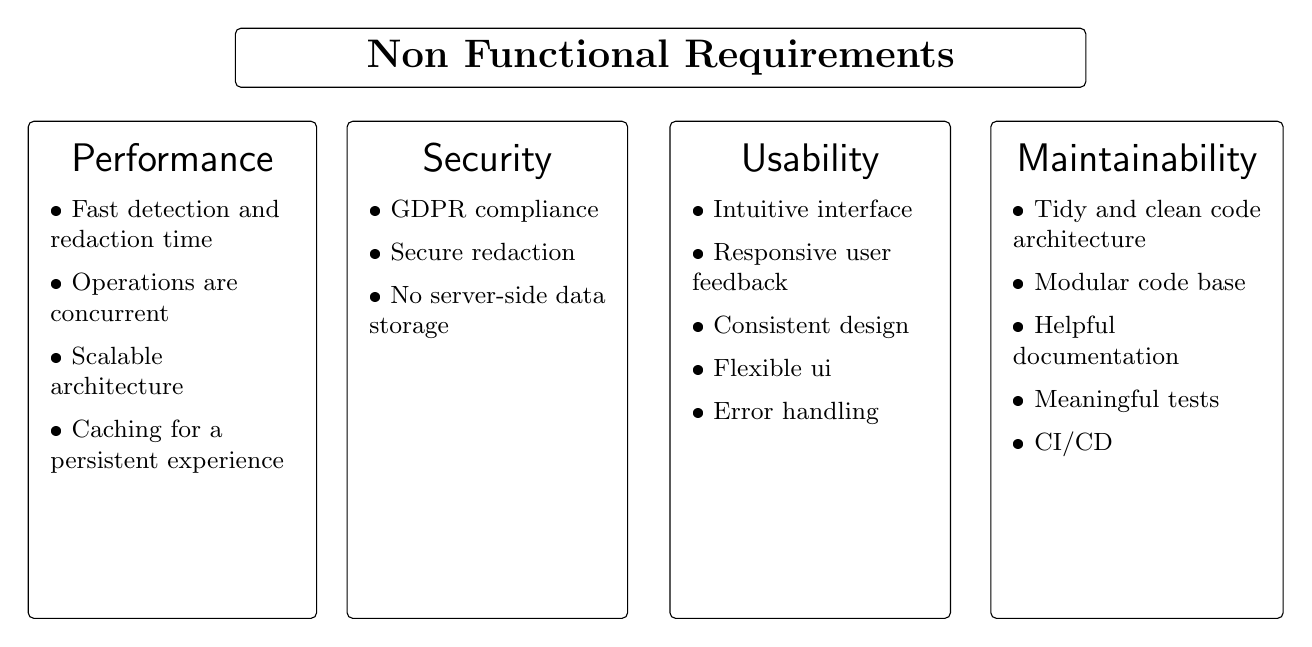
\begin{tikzpicture}[font=\sffamily]

        % Title
        \node[
            draw=black,
            fill=white,
            rounded corners=2pt,
            minimum width=10.8cm,
            minimum height=0.75cm,
            font=\bfseries\Large,
            align=center
        ] at (8.4,7.75) {Non Functional Requirements};

        % Performance
        \node[
            draw=black,
            fill=white,
            rounded corners=2pt,
            anchor=north,
            inner sep=8pt
        ] at (2.2,6.95) {%
            \parbox[t][5.75cm][t]{3.1cm}{%
                {\centering\Large Performance\par}
                \vspace{0.20cm}
                {\normalfont\small\raggedright
                \textbullet\ Fast detection and redaction time\par\vspace{0.16cm}
                \textbullet\ Operations are concurrent\par\vspace{0.16cm}
                \textbullet\ Scalable architecture\par\vspace{0.16cm}
                \textbullet\ Caching for a persistent experience\par}
            }%
        };

        % Security
        \node[
            draw=black,
            fill=white,
            rounded corners=2pt,
            anchor=north,
            inner sep=8pt
        ] at (6.2,6.95) {%
            \parbox[t][5.75cm][t]{3.0cm}{%
                {\centering\Large Security\par}
                \vspace{0.20cm}
                {\normalfont\small\raggedright
                \textbullet\ GDPR compliance\par\vspace{0.16cm}
                \textbullet\ Secure redaction\par\vspace{0.16cm}
                \textbullet\ No server-side data storage\par}
            }%
        };

        % Usability
        \node[
            draw=black,
            fill=white,
            rounded corners=2pt,
            anchor=north,
            inner sep=8pt
        ] at (10.3,6.95) {%
            \parbox[t][5.75cm][t]{3.0cm}{%
                {\centering\Large Usability\par}
                \vspace{0.20cm}
                {\normalfont\small\raggedright
                \textbullet\ Intuitive interface\par\vspace{0.16cm}
                \textbullet\ Responsive user feedback\par\vspace{0.16cm}
                \textbullet\ Consistent design\par\vspace{0.16cm}
                \textbullet\ Flexible \acrshort{ui}\par\vspace{0.16cm}
                \textbullet\ Error handling\par}
            }%
        };

        % Maintainability
        \node[
            draw=black,
            fill=white,
            rounded corners=2pt,
            anchor=north,
            inner sep=8pt
        ] at (14.45,6.95) {%
            \parbox[t][5.75cm][t]{3.15cm}{%
                {\centering\Large Maintainability\par}
                \vspace{0.20cm}
                {\normalfont\small\raggedright
                \textbullet\ Tidy and clean code architecture\par\vspace{0.16cm}
                \textbullet\ Modular code base\par\vspace{0.16cm}
                \textbullet\ Helpful documentation\par\vspace{0.16cm}
                \textbullet\ Meaningful tests\par\vspace{0.16cm}
                \textbullet\ CI/CD\par}
            }%
        };

    \end{tikzpicture}%
    }

    \caption{Overview of Non-Functional Requirements}
    \label{fig:non_functional_req}
\end{figure}

\subsubsection{Security}

Security requirements ensure that sensitive information is handled in a safe and responsible manner. Since the system processes images and videos that may contain personal data, the design should support GDPR-related principles such as data minimization, responsible processing, and reduced unnecessary storage. To support this, uploaded media should only be processed temporarily and should not be stored permanently on the server after the operation is complete. Secure redaction is therefore a central requirement, meaning that sensitive information should be anonymized before the processed output is used further. This reduces the risk of data breaches, unnecessary retention, and exposure of identifiable information while supporting the privacy oriented purpose of the system.

\subsubsection{Performance}

Performance requirements ensure that the system operates efficiently and provides a smooth user experience. Detection and redaction should be completed within a reasonable time so that users do not experience unnecessary delays when processing images or videos. This is especially important because \gls{SafeVision} includes \acrshort{ml} based analysis, which can be computationally demanding depending on the selected detection options, file size, and redaction method. The architecture should also support concurrent operations and be able to handle increasing workloads if the system is expanded further. Caching and client-side state handling can contribute to a more efficient user experience by reducing unnecessary repeated work and preserving relevant workflow information during interactions.

\subsubsection{Usability}

Usability requirements focus on making the system intuitive and understandable for users. Since \gls{SafeVision} is intended to support a workflow involving upload, detection, review, manual correction, redaction, and verification, the interface must make this sequence clear. Users should be able to understand what step they are in, what action is expected next, and whether the system is currently processing or waiting for input.

Responsive feedback is therefore important. Visual indicators, progress feedback, and clear messages help users understand the system state and the results of their actions. A consistent design across the application also makes navigation more predictable and reduces confusion. In addition, the interface should support flexibility by allowing users to adjust detection results, choose redaction methods, and correct errors before final output. Clear error handling is also necessary so that users can recover from issues without losing track of the workflow.

\subsubsection{Maintainability}

Maintainability requirements ensure that the system can be developed, updated, and extended over time. \gls{SafeVision} consists of several connected parts, including frontend interaction, backend services, \acrshort{ml} models, redaction logic, video processing, and deployment configuration. A modular codebase is therefore important because it separates responsibilities and makes it easier to modify one part of the system without affecting unrelated functionality.

Clean code structure, helpful documentation, and meaningful tests support long-term maintainability. Documentation makes the system easier to understand for new contributors, while tests help verify that important functionality continues to work when changes are introduced. CI/CD practices further support maintainability by enabling regular validation and deployment of updates. These requirements are important because the system should be designed in a way that allows for future improvement and extension.

%------------------------- 4.4 ---------------------------

\section{Requirement Prioritization}
\label{sec:priority}

To guide development and ensure that critical functionality was implemented first, the requirements were prioritized based on their importance, impact on the system, and input from Safe Media AI. The prioritization reflects a practical development approach, where essential functionality was implemented first, followed by desirable features, while less critical functionality was considered for potential future work.

\begin{itemize}
    \item \textbf{High Priority:}
    \begin{itemize}
        \item Automatic detection of sensitive information
        \item Manual editing capabilities
        \item Redaction functionality
        \item Image format support (PNG/JPEG)
    \end{itemize}

    \item \textbf{Medium Priority:}
    \begin{itemize}
        \item Multiple redaction methods
        \item Fast processing performance
        \item Video capabilities
    \end{itemize} 

    \item \textbf{Lower Priority:}
    \begin{itemize}
        \item Text Recognition capabilities
        \item Advanced customization options
        \item Inpaint redaction method
        \item Complex user preference options
        \item Metadata extraction and flexibility
    \end{itemize}
\end{itemize}


\chapter{System Architecture}

\section{System Architecture Overview}
\label{system_architecture_overview}
The system is designed as a modular client-server architecture for detecting and redacting sensitive content in both still images and video. At a high level, the architecture consists of a frontend, a backend/API layer, and separate processing components for detection and redaction.

\begin{figure}[H]
    \centering
    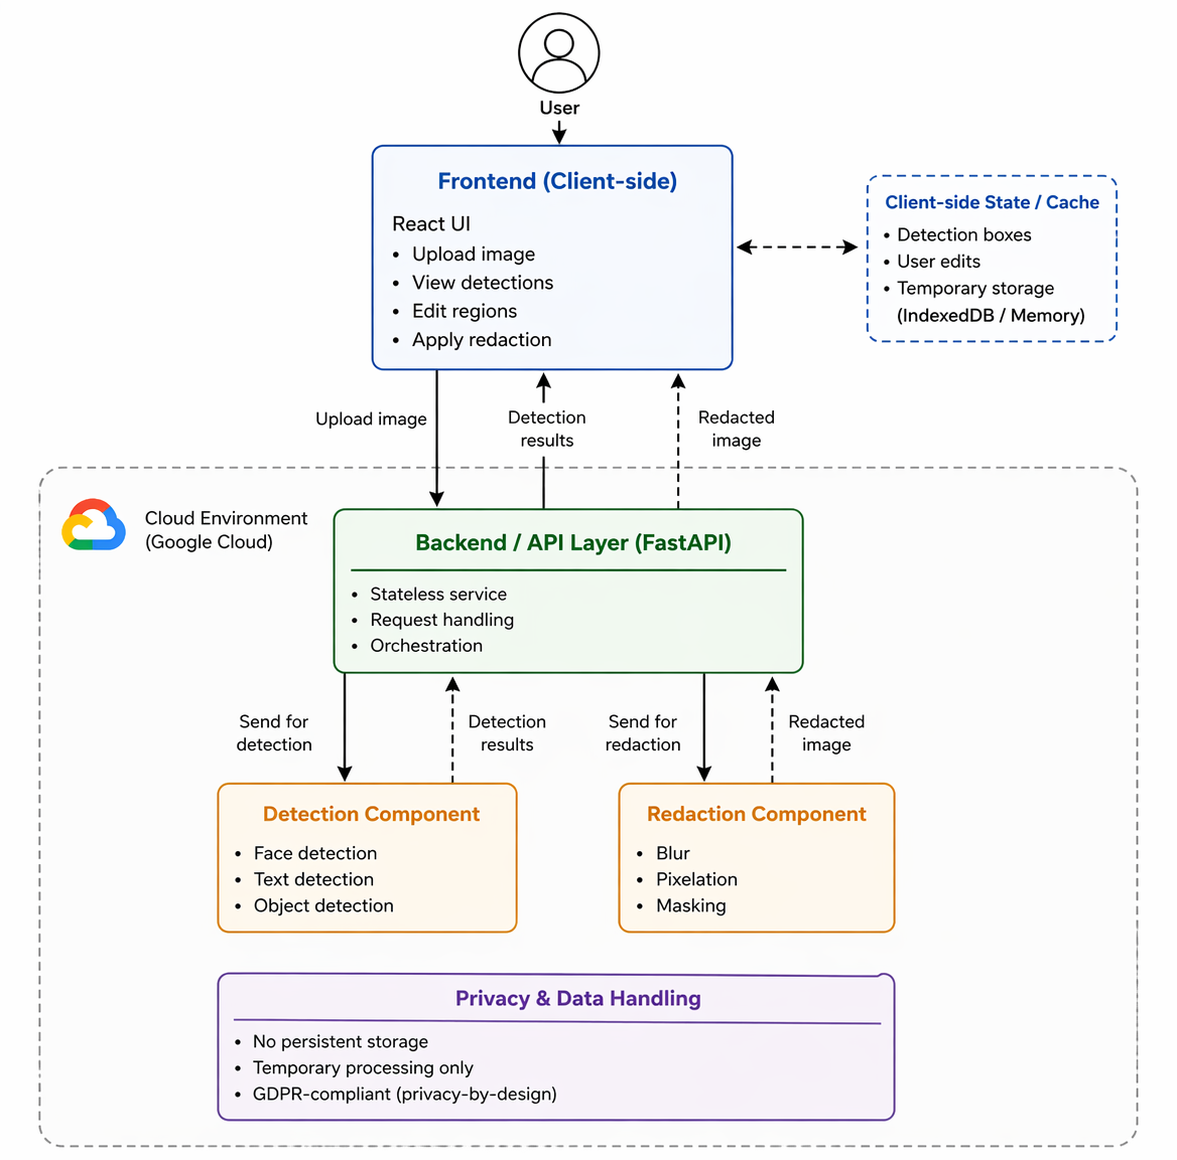
\includegraphics[width=0.85\textwidth]{figures/images/chapter-5/SystemArchitectureOverview.png}
    \caption{High-level system architecture of the proposed solution. Created by the authors, with AI-assisted refinement.}
    \label{fig:system_architecture_overview}
\end{figure}

Figure~\ref{fig:system_architecture_overview} provides an overview of the main architectural elements and their relationships. The following subsections describe the design principles and system components in more detail.

\methodheading{Architectural Design}
\label{architecture_design}
The system follows a layered architectural design, where each layer has a specific responsibility and communicates with adjacent layers. This design reduces system complexity and enables independent development of components \cite{shaw1996software}. It also simplifies debugging and testing, as each layer can be evaluated in isolation.

\begin{itemize}
    \item \textbf{Presentation Layer (Frontend):} Handles user interaction and displays results.
    \item \textbf{Application Layer (Backend):} Manages requests and coordinates processing.
    \item \textbf{Processing Layer:} Performs detection and redaction operations.
\end{itemize}

\methodheading{Design Principles}
\label{design_principles}
The architecture is guided by several design principles to ensure robustness and long-term maintainability.

A client-server architecture is used to separate user interaction from processing
logic. The client is responsible for the user interface, while the server handles
data processing and computational tasks \cite{clientserverUW}. This separation allows
computationally intensive operations, such as machine learning inference, to be
performed on the server side.

Separation of concerns is applied by assigning distinct responsibilities to each component. In particular, detection and redaction are implemented as separate modules, allowing improvements to one part of the pipeline without affecting the other. This reduces coupling and simplifies future extensions \cite{martin2017}.

Modularity is emphasized to support extensibility. For example, the detection module can be replaced or upgraded as new machine learning models become available, without requiring changes to the frontend or backend interfaces. This follows principles of modular design and loose coupling, improving maintainability and flexibility \cite{martin2017}.

The backend is designed to be stateless, meaning that each request is processed
independently. As a result, deployment is simplified and the system can scale
horizontally by distributing requests across multiple instances \cite{aws_stateless}.

Privacy is a key design consideration. By avoiding persistent storage of sensitive
data, the system minimizes the risk of data exposure and aligns with data
minimization principles defined in the GDPR \cite{gdpr}. This introduces a trade-off, as features such as history tracking or persistent sessions are limited, but this was considered
acceptable given the sensitivity of the processed data.

Overall, the chosen architecture reflects a balance between performance, usability, and privacy, where real-time interaction and user control are prioritized over fully automated processing.

\section{System Components}

Section~\ref{system_architecture_overview} presented the system from a layered architectural perspective. This section complements that view by describing the system in terms of functional components and their responsibilities.

The system consists of four primary components: the User Interface (UI), the Detection component, the Redaction component, and the API layer. These components are designed according to the principles discussed in
Subsection~\ref{design_principles}.

\methodheading{User Interface (UI)}

The User Interface (UI) is a web-based frontend responsible for presenting
detection results and enabling user interaction with the system. It serves as the
primary point of interaction between the user and the processing pipeline.

A central aspect of the UI is the workspace, which provides an interactive view
of uploaded images and detected regions. Users can inspect and validate detection
results before redaction is applied, supporting a human-in-the-loop workflow.
This is further discussed in Chapter~\ref{user_interface_and_usability}.

The UI communicates with the backend through the API layer and presents processed results to the user. It is responsible for maintaining a consistent interaction state as detection results are reviewed or redaction is applied.

The UI supports the privacy-oriented design described in
Subsection~\ref{design_principles} by handling sensitive user data primarily on the client side.

\methodheading{Detection and Redaction Component}

A central backend processing component in the system is organized around two
main workflows: detection and redaction. As illustrated in
Figure~\ref{fig:api_workflows}, these workflows follow the same overall
structure for both still images and video. In both cases, the media is processed
through the same core stages for analysis, sensitive-region identification, and
redaction. The main difference is that video processing operates across multiple
frames, and the frame-level results must be accumulated before being returned to
the frontend.

Figure~\ref{fig:api_workflows}(a) shows the high-level detection workflow. After
input media is received by the API, it is decoded and may optionally undergo
preprocessing. The media is then passed to multiple detection components, which
can operate in parallel. Their outputs are subsequently normalized into a
consistent format before being returned through the API layer. For still images,
this produces a direct detection result. For video, the same workflow is applied
to relevant frames, and the frame-level detections are collected into a unified
response.

\begin{figure}[H]
\centering

\begin{subfigure}[t]{0.48\textwidth}
    \centering
    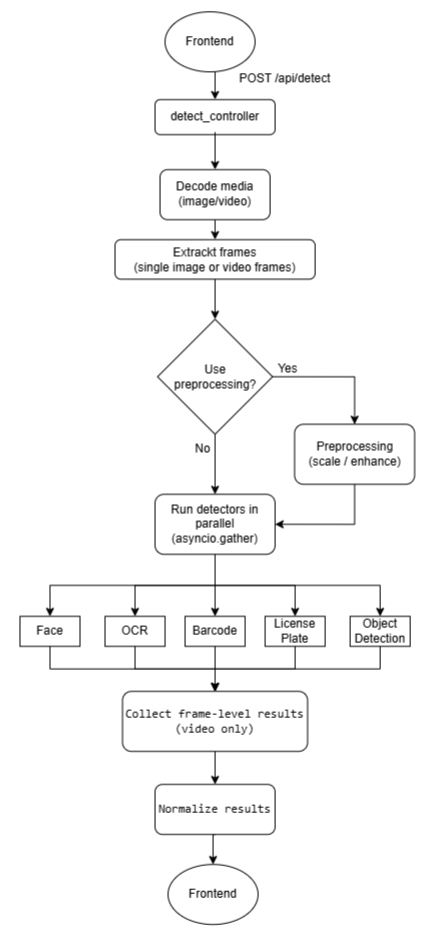
\includegraphics[width=\textwidth]{figures/images/chapter-5/detection-api-flow-v2.png}
    \caption{Detection pipeline showing image processing, optional preprocessing, parallel execution of detection models, and result normalization.}
    \label{fig:detection_api_flow_v2}
\end{subfigure}
\hfill
\begin{subfigure}[t]{0.48\textwidth}
    \centering
    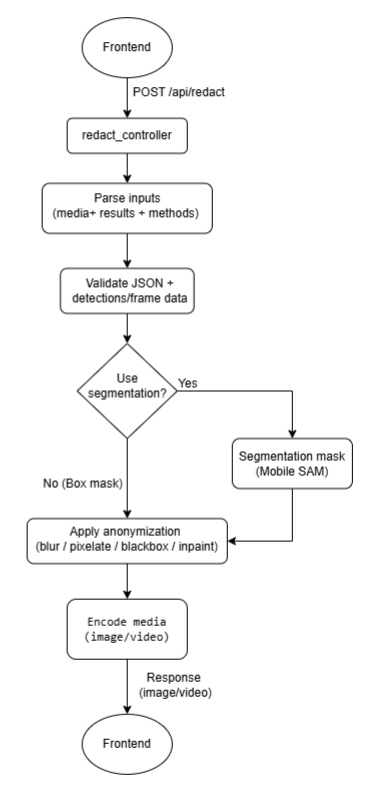
\includegraphics[width=\textwidth]{figures/images/chapter-5/redaction-api-flow-v2.png}
    \caption{Redaction pipeline showing input validation, optional segmentation, and application of anonymization techniques.}
    \label{fig:redaction_api_flow_v2}
\end{subfigure}

\caption{Overview of detection and redaction workflows in the backend system.}
\label{fig:api_workflows}
\end{figure}

Rather than applying redaction automatically, the detection results are sent to
the UI for user review and adjustment. This improves reliability in cases where
automated detection may be incomplete or imprecise.

Figure~\ref{fig:api_workflows}(b) shows the corresponding redaction workflow.
In this stage, the backend receives both the input media and the validated
detection results, applies input validation, and executes the selected
anonymization method. Depending on the selected strategy, redaction may be
based on bounding boxes or segmentation masks. For still images, redaction is
applied directly to the image. For video, the same workflow is applied frame by
frame, after which the processed frames are recombined into the final redacted
video.

This design makes it possible to separate detection from redaction as two
independent but connected stages. Such a separation improves modularity and
also allows detection results to be reused for visualization, inspection, or
later anonymization.

\methodheading{API Layer}

The API layer defines the communication interface between the frontend and the
backend processing components. It exposes detection and redaction functionality
through well-defined endpoints, allowing the UI to interact with the processing
pipeline without depending on its internal implementation. The API follows the
stateless and privacy-oriented design principles described in
Subsection~\ref{design_principles}.

The API is organized using a modular structure in which different tasks are
handled by dedicated controllers. In particular, detection and redaction are
exposed through separate routes, which improves maintainability and helps
distinguish between different processing tasks, including image-based and
video-based workflows.

\begin{figure}[H]
\centering
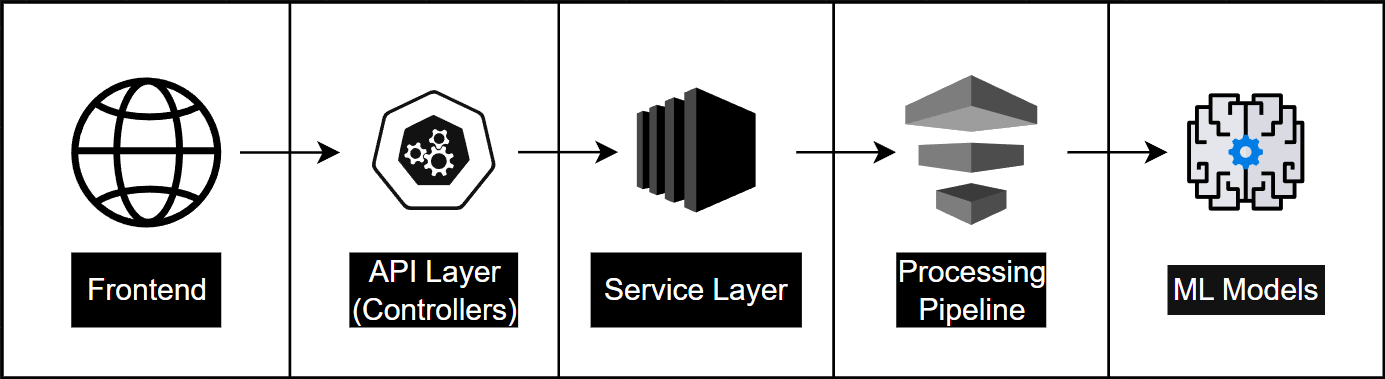
\includegraphics[width=14cm]{figures/images/chapter-5/backend_architecture_diagram.png}
\caption{Overview of the backend architecture showing the API layer, service layer, processing pipeline, and machine learning components.}
\label{fig:backend_architecture_diagram}
\end{figure}

The frontend communicates with the API layer, which forwards
requests to the service layer and the underlying processing pipeline (Figure~\ref{fig:backend_architecture_diagram}).
This reflects a layered design in which request handling, application logic, and
machine learning inference are separated into distinct responsibilities.


\methodheading{Machine Learning Development Process}

In addition to the deployed application components, the project also included a
separate development process for custom machine learning models. This process was required for the barcode and license plate detectors, as well
as the custom NER model used for text classification in the system, and formed an important part of the overall solution architecture.

As illustrated in Figure~\ref{fig:ml_pipeline}, the process consists of dataset
preparation, model training, evaluation, and deployment. In practice, this
meant that datasets had to be collected and standardized, models had to be
trained and evaluated in a dedicated development environment, and selected model
artifacts were then integrated into the SafeVision backend for inference.

\begin{figure}[H]
\centering
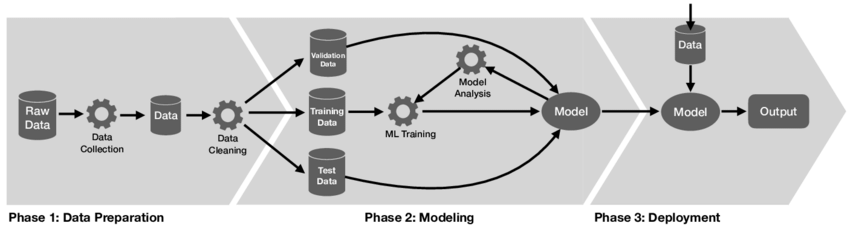
\includegraphics[width=0.9\textwidth]{figures/images/chapter-5/machine-learning-pipeline.png}
\caption{General machine learning pipeline consisting of data preparation, model training, evaluation, and deployment phases (adapted from \cite{ml_pipeline_source}).}
\label{fig:ml_pipeline}
\end{figure}

This development process was kept separate from the deployed application in
order to reduce coupling between experimental model development and the
production-oriented system. While the SafeVision application is responsible for
inference, redaction, and user interaction, the machine learning development
process focuses on preparing data, training models, and validating model
performance before integration into the deployed backend.

The technical tools, environments, and repository structure used to support this
process are described in Chapter~\ref{chap:technologies_and_methodologies}, while the
concrete implementation of dataset preparation, training, and model integration
is presented in Chapter~\ref{chap:implementation_details}.


\section{Deployment Architecture}

The deployment architecture describes how SafeVision is made available as a
web-based system and how its main components are organized in operation. In
line with the overall client--server architecture, the system is deployed as two
separate parts: a browser-based frontend client and a backend service
responsible for API handling and processing tasks. The backend handles
detection, redaction, and related processing tasks for both still images and
video. This includes model inference, redaction processing, and media-specific
workflow handling.

\begin{figure}[H]
\centering
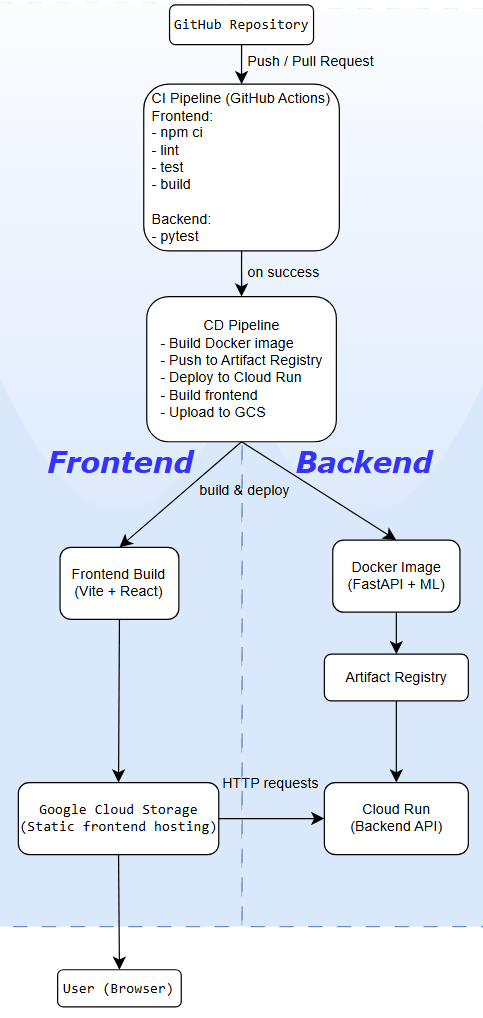
\includegraphics[width=0.5\textwidth]{figures/images/chapter-5/deployment-architecture.png}
\caption{Deployment architecture and CI/CD pipeline.}
\label{fig:deployment_architecture}
\end{figure}

Figure~\ref{fig:deployment_architecture} illustrates the deployment architecture
at a structural level. The frontend provides the user-facing interface and
communicates with the backend through HTTP-based API requests. By separating
presentation and interaction concerns from processing and inference, the system
becomes easier to maintain, update, and extend over time.

The deployment design also reflects the architectural principles presented
earlier in this chapter. In particular, the backend is treated as an isolated
service environment for processing and inference, while the frontend remains
focused on interaction and presentation. This supports modularity and reduces
coupling between the user interface and the underlying processing pipeline.
More specific technologies and infrastructure choices used to realize this
deployment are described in Chapter~\ref{chap:technologies_and_methodologies}.
\chapter{\acrshort{ui} and Usability}
\label{user_interface_and_usability}

The final \gls{SafeVision} \acrshort{ui} is presented in this Chapter, with emphasis on how it supports the hybrid redaction workflow. The interface was developed to remain consistent with Safe Media AI's existing platform while adapting the workflow to visual media. Further discussion of the UI theory, design principles, and interface evolution is provided in Appendix~\ref{app:depth_ui_ux}.

\section{Interface Design and Components}

As shown in Figure~\ref{fig:ui_final_examples} (a), the interface starts in an intentionally minimal state. Before files are uploaded, users are presented with a clear upload action and an empty file panel. By avoiding unnecessary controls before they become relevant, the design supports simplicity. Once files are uploaded, the interface expands into the full editing workspace shown in Figure~\ref{fig:ui_final_examples} (b).

On the left side, the file panel gives users an overview of uploaded images and videos. Each file item displays basic information such as file name and file type. During longer operations, individual progress indicators can also be shown for each file, as illustrated in Figure~\ref{fig:file_progress}. Providing this feedback improves system state awareness, especially when \gls{SafeVision} processes several files and users need to understand which file is selected, which task is running, and how far the operation has progressed.

\begin{figure}[H]
\centering

\includegraphics[width=0.55\textwidth]{figures/images/chapter-6/uikomp01.png}
\caption{File item showing individual progress feedback during processing.}
\label{fig:file_progress}
\end{figure}

At the center of the interface, the workspace functions as the main interaction area. Uploaded images and videos are displayed in the middle of the screen so users can inspect the visual content being processed without switching between separate views. By showing detection results directly on the media, the interface reduces the need to compare separate lists or external outputs, which helps lower cognitive load. After identification is completed, detected regions appear as labeled \gls{bounding box}es on the image or video frame, as shown in Figures~\ref{fig:ui_final_examples} (c) and~\ref{fig:video_detection_results}. Using overlays and labeled \gls{bounding box}es reflects the principle of visual feedback \cite{norman2013design}. Detection results appear directly where the sensitive content is located, making the system output easier to understand. As a result, users can assess whether the detected regions are correct, remove \gls{false positive}s, or add missing regions manually.

%----------------
\begin{figure}[H]
    \centering

    \begin{minipage}{\textwidth}
        \centering
        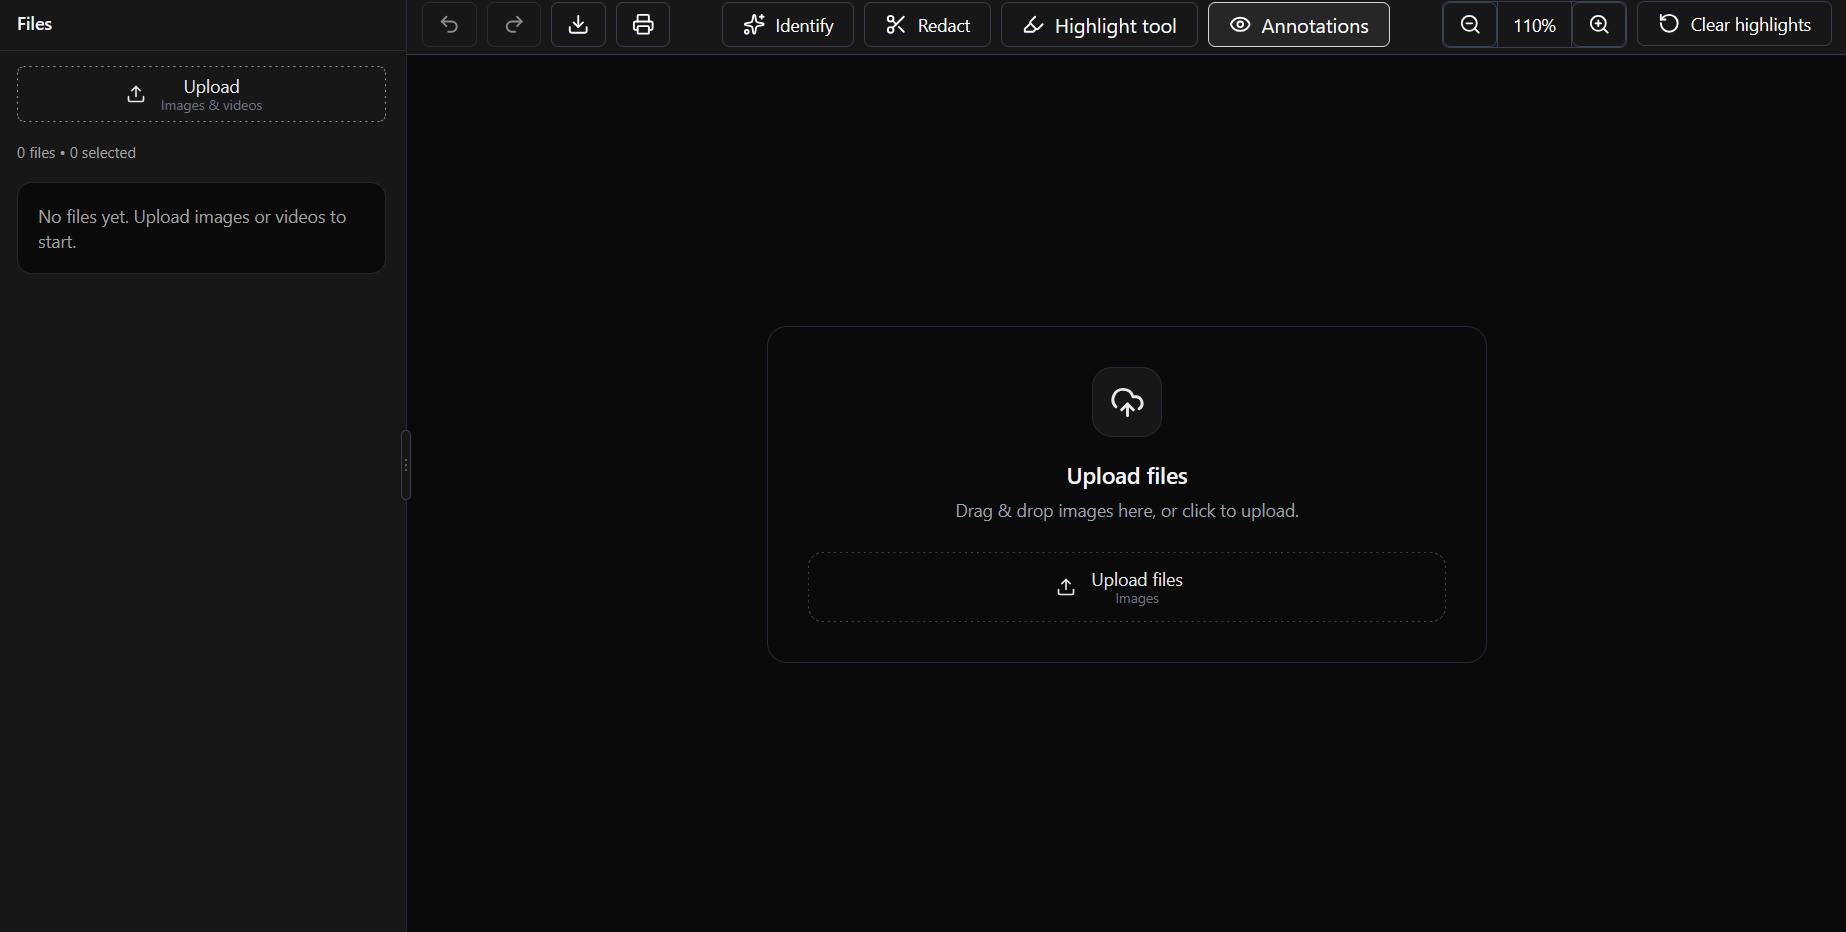
\includegraphics[width=0.7\textwidth]{figures/images/chapter-6/uislutt01.png}
        \par\vspace{2pt} \small (a) Final interface in its initial state before files are uploaded.
    \end{minipage}

    \vspace{0.0cm}

    \begin{minipage}{\textwidth}
        \centering
        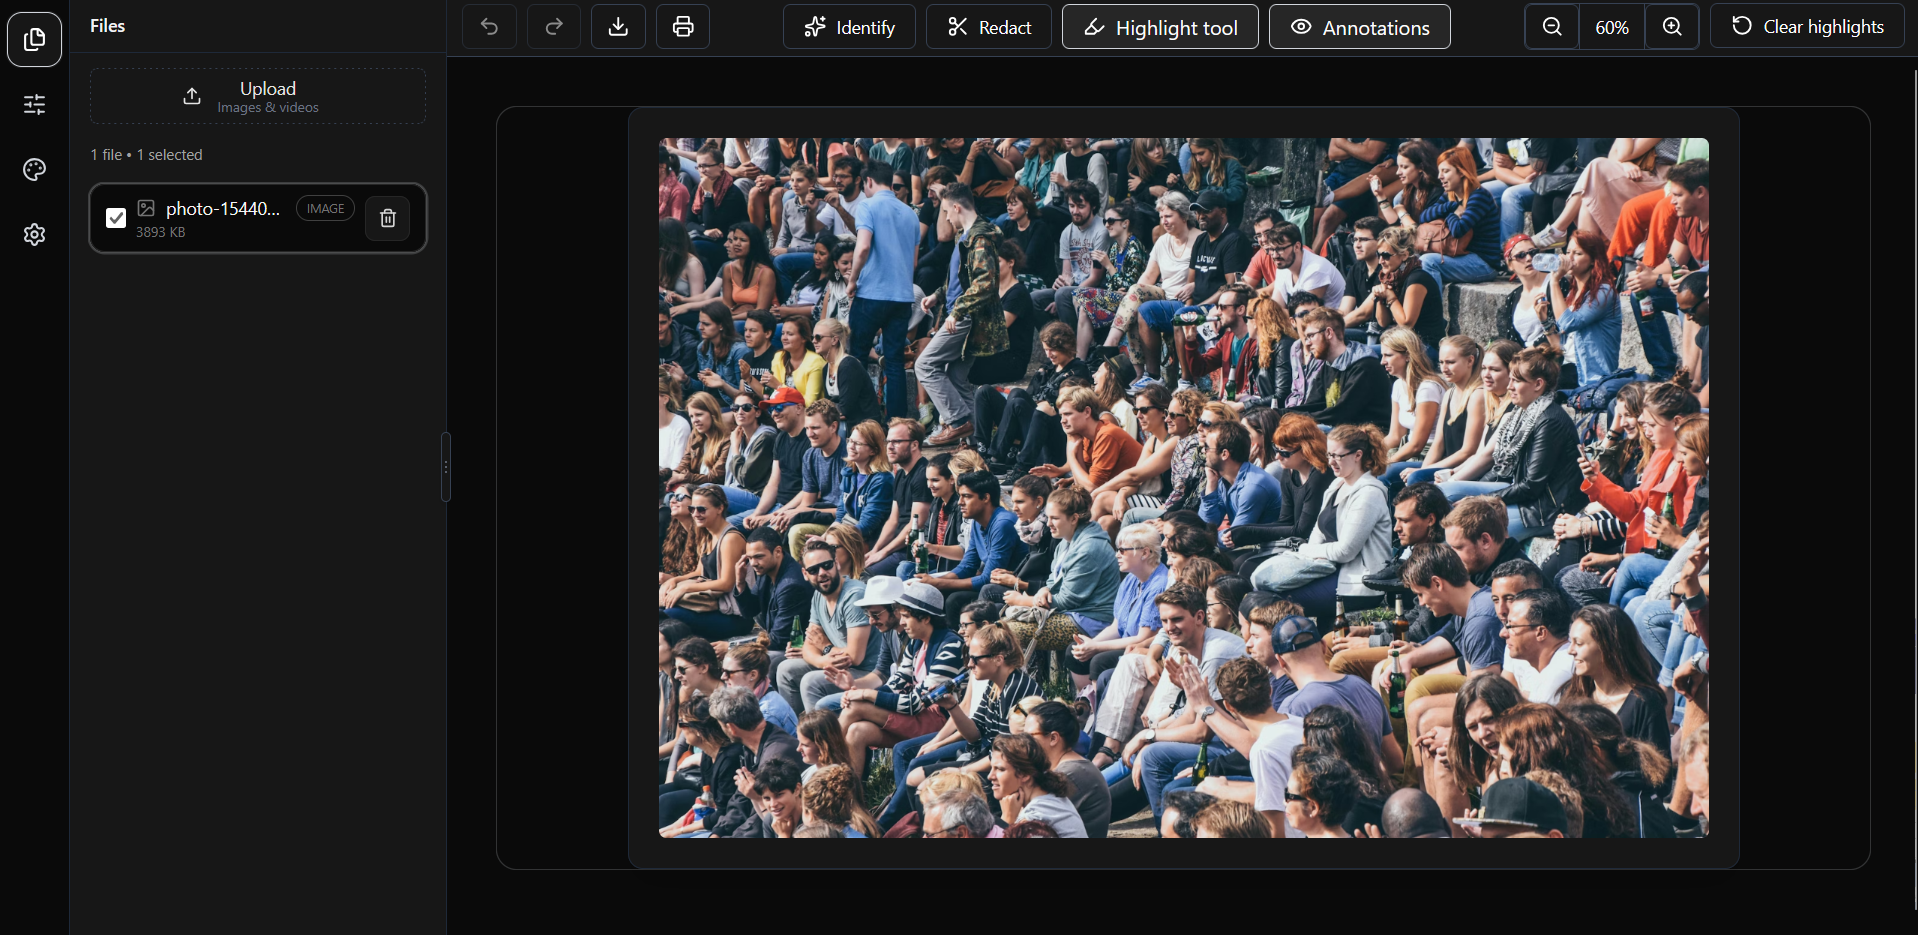
\includegraphics[width=0.7\textwidth]{figures/images/chapter-6/uislutt02.png}
        \par\vspace{2pt} \small (b) Final image workspace with uploaded media displayed in the central viewer.
    \end{minipage}

    \vspace{0.0cm}
    
    \begin{minipage}{\textwidth}
        \centering
        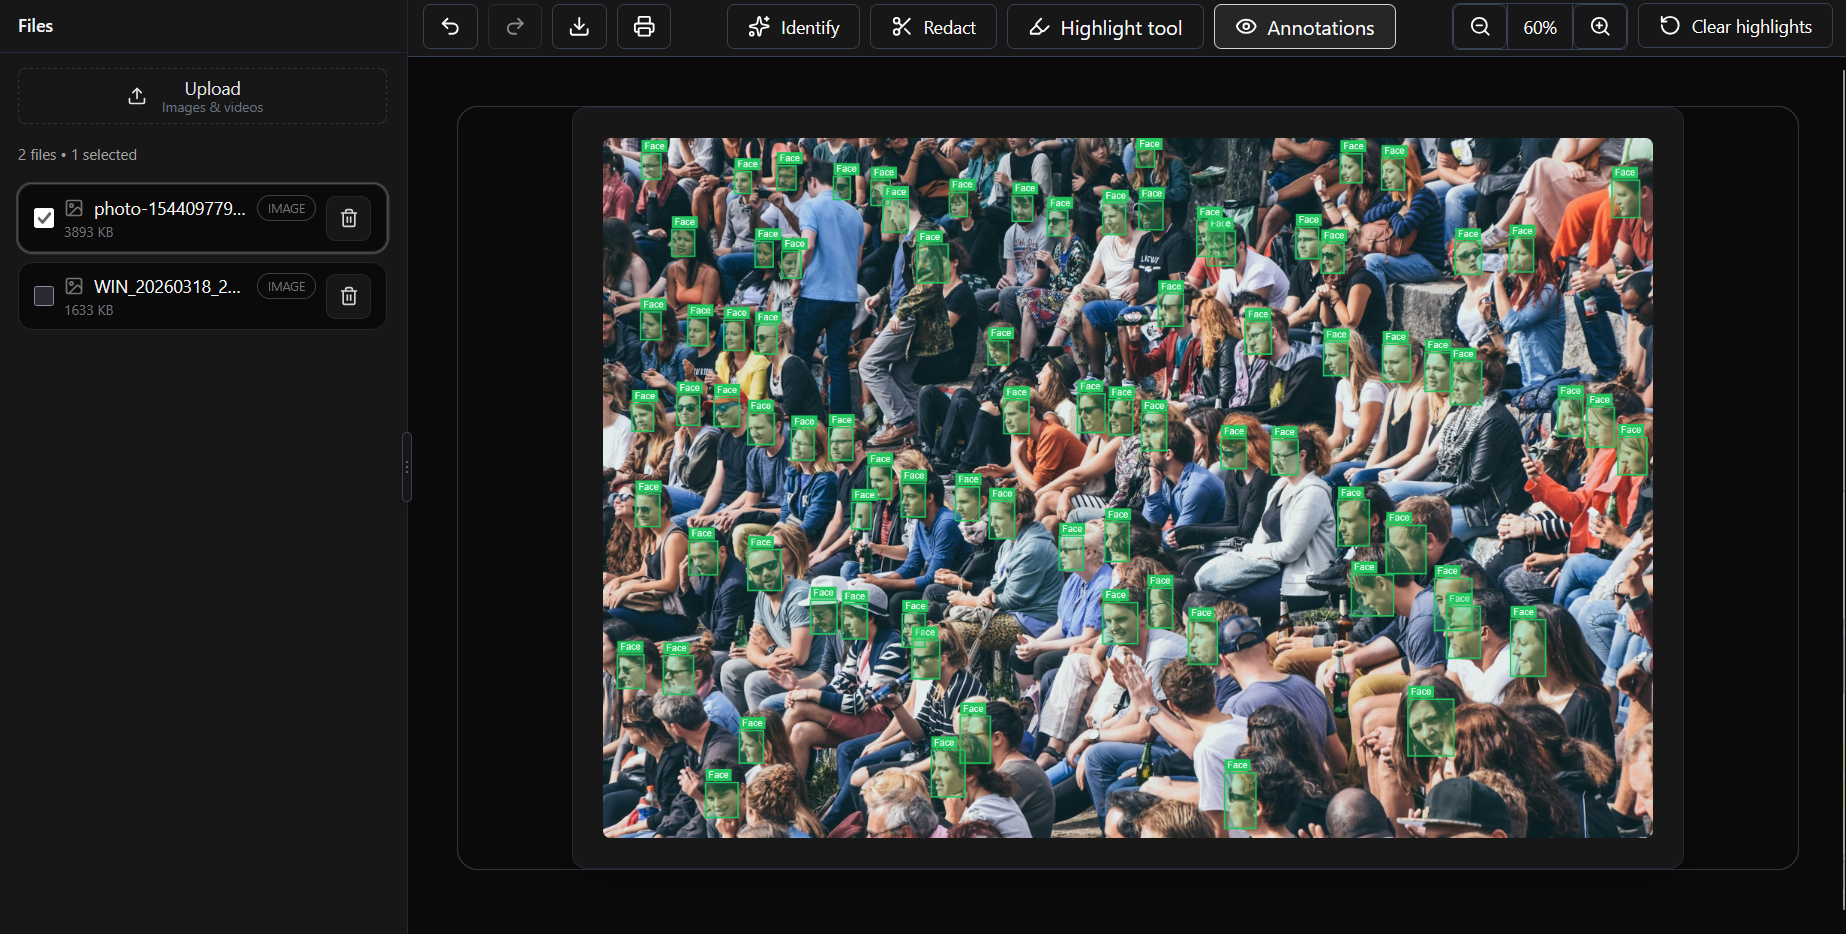
\includegraphics[width=0.7\textwidth]{figures/images/chapter-6/uislutt03.png}
        \par\vspace{2pt} \small (c) Detection results displayed directly on the image using labelled \gls{bounding box}es.
    \end{minipage}

    \caption{Examples of the finalinterface across different stages of the image workflow, from the initial state to uploaded media and displayed detection results. The image used in the workspace examples is from Guillemot~\cite{guillemot_stadium}}
    \label{fig:ui_final_examples}
\end{figure}
%----------------
 
Primary actions are placed in the top toolbar to reflect the intended workflow. By keeping these controls consistently above the workspace as illustrated in Figure~\ref{fig:ui_final_examples}, the main workflow remains visible and predictable throughout the redaction process. 

As shown in Figure~\ref{fig:options_panel_components} (a), secondary and advanced settings are placed in the side panel. Instead of showing every configuration option in the main workspace, settings related to both image and video handling are grouped separately. Advanced functionality therefore remains available without overwhelming the basic workflow, which supports progressive disclosure \cite{nielsen2020progressive}. In practice, this keeps the interface simple for new users while still giving more experienced users additional control when needed. Detection filters allow users to choose which categories should be identified (b). This gives the users flexibility over the hybrid workflow. The same design logic is also applied for video options, Figure~\ref{fig:options_video_rate}. The interface therefore includes components for image visualization, control panels, and editing tools, enabling users to inspect detected regions and apply redaction methods while maintaining clarity and responsiveness, which are central usability principles \cite{usability_nielsen}.

\begin{figure}[H]
\centering

\begin{subfigure}[t]{0.32\textwidth}
    \centering
    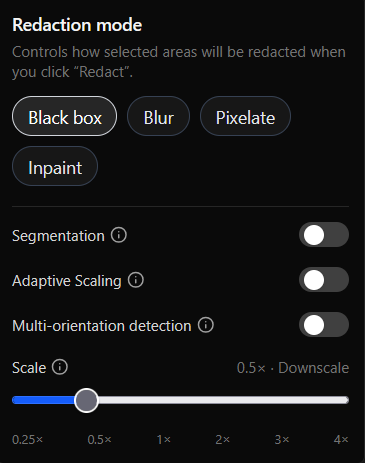
\includegraphics[width=\textwidth]{figures/images/chapter-6/uikomp05.png}
    \caption{Redaction mode and processing settings.}
    \label{fig:options_redaction_mode}
\end{subfigure}
\hfill
\begin{subfigure}[t]{0.32\textwidth}
    \centering
    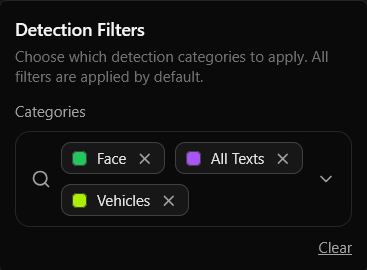
\includegraphics[width=\textwidth]{figures/images/chapter-6/uikomp06.png}
    \caption{Detection filters.}
    \label{fig:options_detection_filters}
\end{subfigure}
\hfill
\begin{subfigure}[t]{0.32\textwidth}
    \centering
    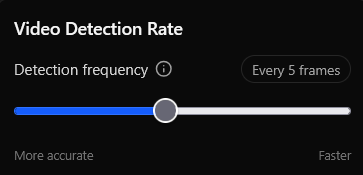
\includegraphics[width=\textwidth]{figures/images/chapter-6/uikomp07.png}
    \caption{Video detection rate.}
    \label{fig:options_video_rate}
\end{subfigure}

\caption{Main components of the options panel. The panel provides access to redaction modes and processing settings, detection filters, and video detection rate configuration.}
\label{fig:options_panel_components}
\end{figure}

Figure~\ref{fig:highlight_styles} (a), the highlight style panel controls how \gls{bounding box}es are displayed. Such customization is important because \gls{SafeVision} may be used on complex images or videos where one default highlight style may not always be readable. Customizable highlighting therefore improves visual feedback and accessibility during detailed inspection tasks.

\begin{figure}[H]
\centering

\begin{subfigure}[t]{0.32\textwidth}
    \centering
    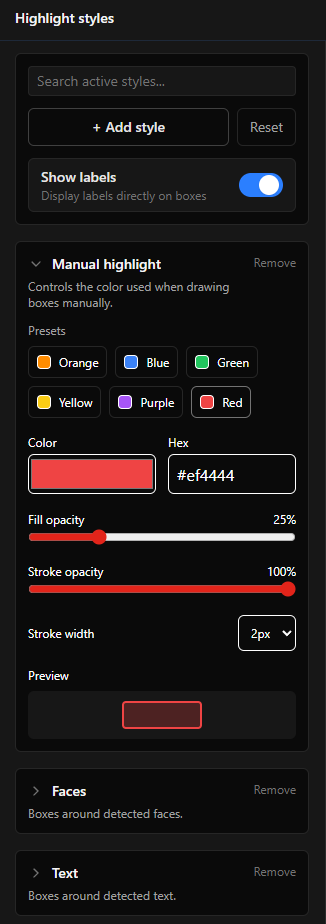
\includegraphics[width=\textwidth]{figures/images/chapter-6/uikomp03.png}
    \caption{Highlight style panel for customizing labels, colors, opacity, and category-specific styles.}
    \label{fig:highlight_styles}
\end{subfigure}
\hfill
\begin{subfigure}[t]{0.32\textwidth}
    \centering
    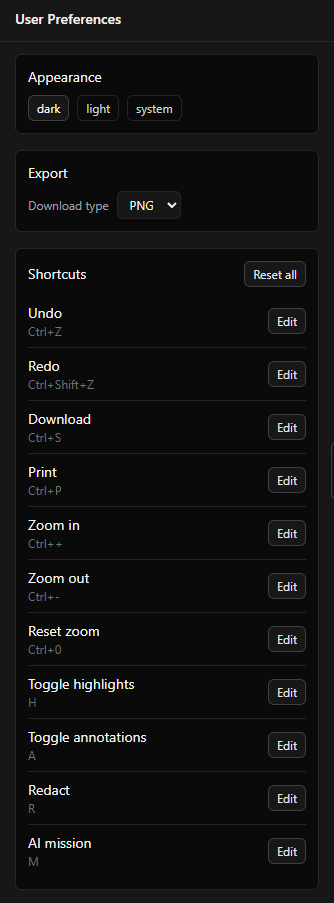
\includegraphics[width=\textwidth]{figures/images/chapter-6/uikomp04.png}
    \caption{User preferences panel with appearance settings, export format, and keyboard shortcuts.}
    \label{fig:user_preferences}
\end{subfigure}

\caption{Configuration panels for highlight styling and user preferences.}
\label{fig:ui_configuration_panels}
\end{figure}

Additional flexibility is provided through the user preferences panel, shown in Figure~\ref{fig:user_preferences}. Users can adapt the interface to different working conditions and make frequent actions faster through personalized settings. At the same time, important functionality remains available through visible interface controls, so the system does not depend on shortcut use. In this way, the preferences panel supports both accessibility and learnability.

Video support extends the same workspace principles to temporal media. As shown in Figure~\ref{fig:video_workspace}, videos are displayed in the central viewer with playback controls, while the surrounding interface remains consistent with the image workflow. After identification, detected regions can be shown on the video frame, as illustrated in Figure~\ref{fig:video_detection_results}. This consistency helps users transfer knowledge from image redaction to video redaction. At the same time, video introduces additional complexity because detections must be interpreted across frames, making clear visual feedback and playback control especially important.

\begin{figure}[H]
\centering

\begin{subfigure}[t]{0.95\textwidth}
    \centering
    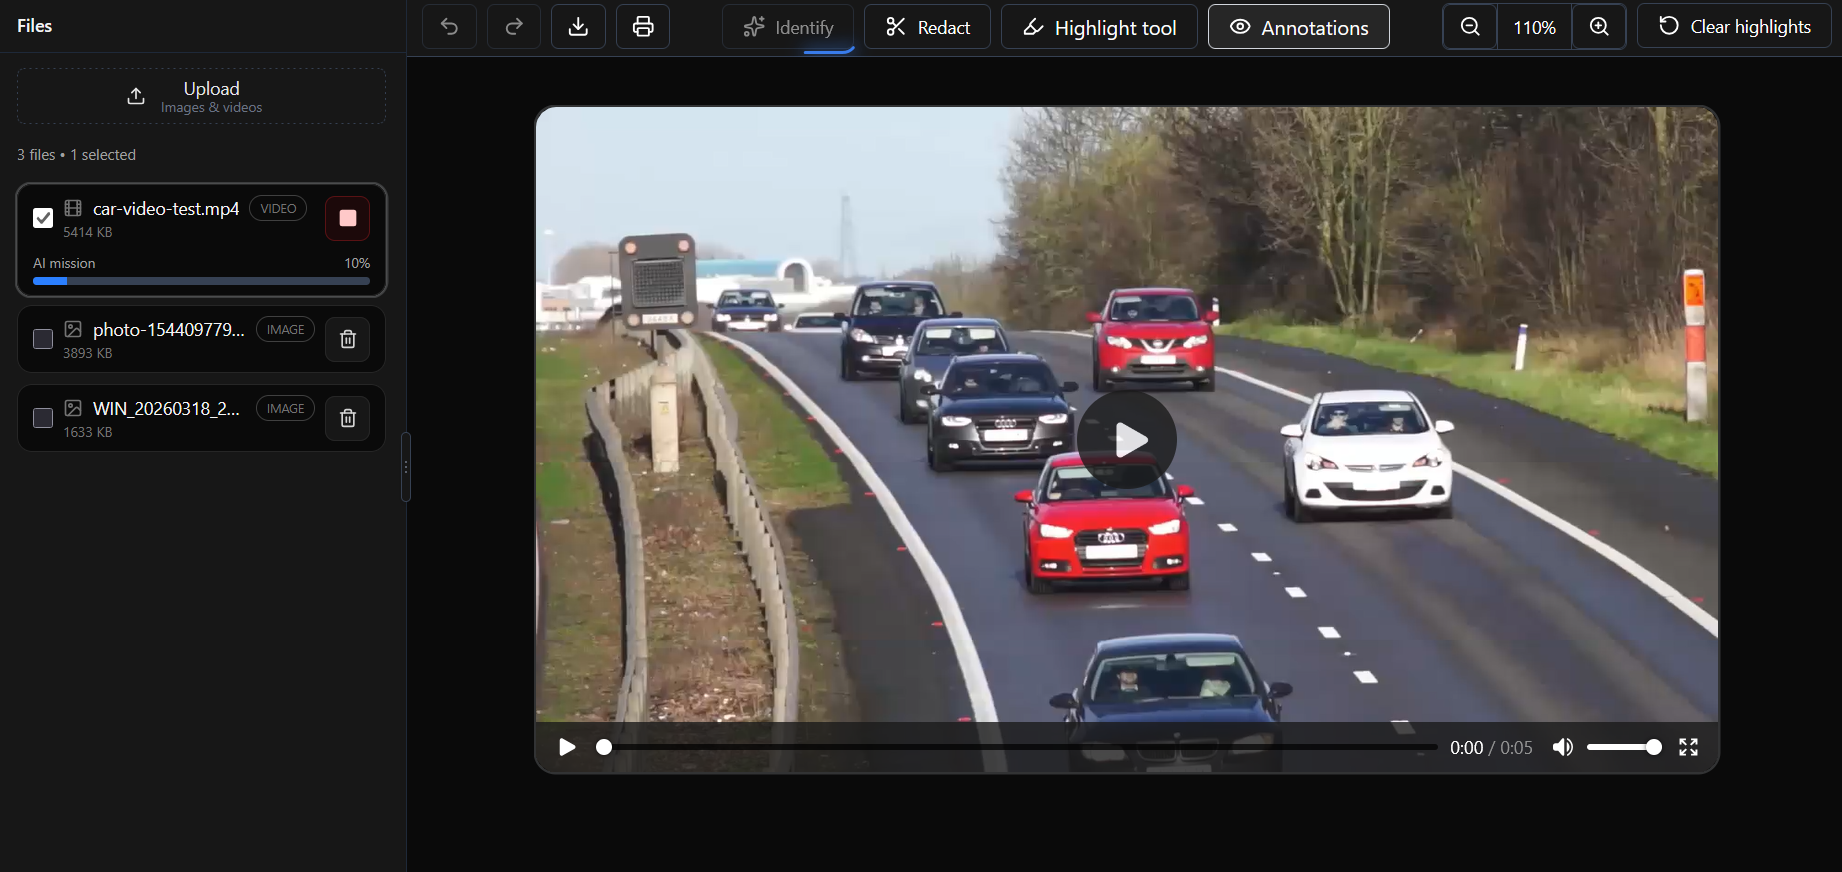
\includegraphics[width=\textwidth]{figures/images/chapter-6/uislutt04.png}
    \caption{Video workspace showing uploaded video content in the central viewer.}
    \label{fig:video_workspace}
\end{subfigure}

\vspace{0.2cm}

\begin{subfigure}[t]{0.95\textwidth}
    \centering
    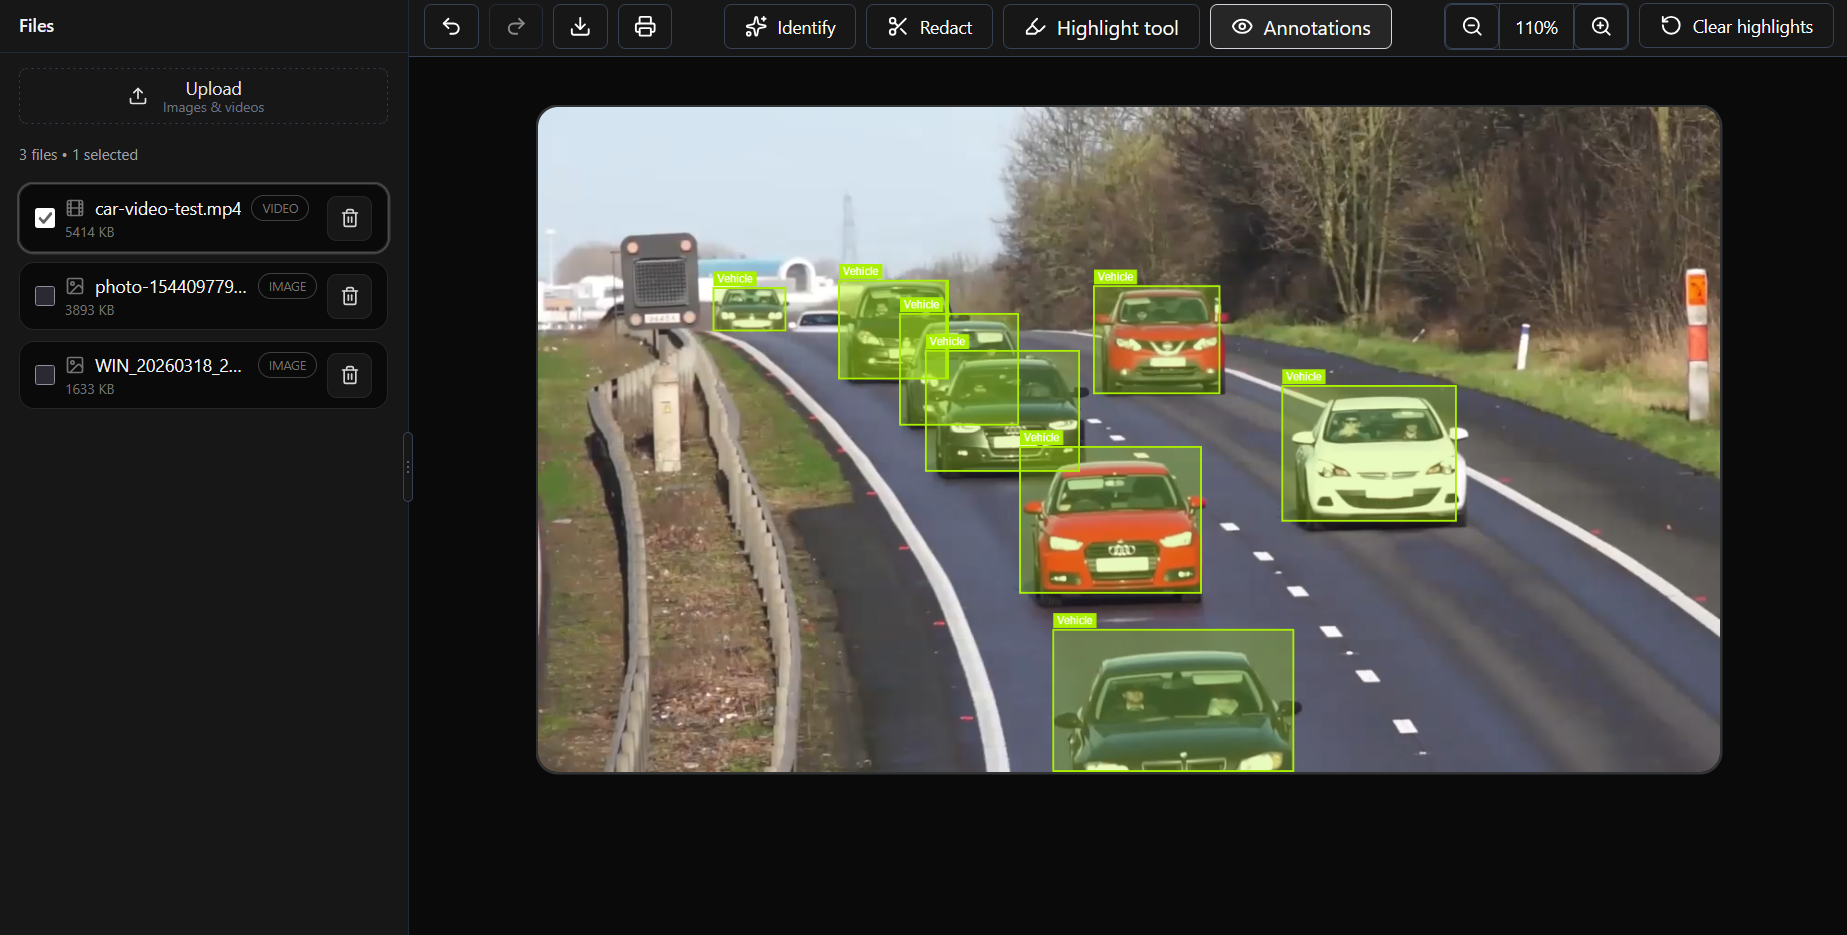
\includegraphics[width=\textwidth]{figures/images/chapter-6/uislutt05.png}
    \caption{Detected vehicle regions displayed on a video frame.}
    \label{fig:video_detection_results}
\end{subfigure}

\caption{Examples of the final \gls{SafeVision} video workflow, showing uploaded video content and detected vehicle regions. The video used in the workspace examples is from ~\cite{pexels_highway_video}.}
\label{fig:video_workflow_examples}
\end{figure}

In the final interface, the design principles described in the previous subsections are applied to the practical needs of \gls{SafeVision}. A single workspace layout keeps the main workflow in one place, while editable detections and configurable settings allow users to stay in control of automated results. Feedback during detection and redaction is provided directly through the interface, and consistent toolbar and panel structures make the workflow more predictable across both image and video processing. Together, these design choices support \gls{SafeVision}'s main goal of combining automated detection with user-guided refinement, so that sensitive visual content can be identified, verified, and redacted in an efficient and controlled workflow.

\section{User Guidance and System Communication}
\label{sec:user_guidance_system_communication}

In addition to the main redaction workflow, the interface includes supporting elements for user guidance and system communication. A short Terms of Service dialog is shown before users begin processing content. This informs users that automated redaction may be inaccurate or incomplete, and that they remain responsible for reviewing results before sharing or publishing processed media. The full Terms of Service text is included in Appendix~\ref{app:terms_of_service}. This was included to make the limitations of automated redaction clearer and to support the responsible use of the system.

The interface also includes a compact patch notes dialog that summarizes important changes between versions, such as performance improvements, image processing changes, video support, and detection updates. This helps communicate system changes to users without requiring them to inspect technical documentation. The patch notes were kept short and limited on user visible changes, since their purpose is to support transparency rather than provide a detailed development log. Examples of these supporting dialog are shown in Figure~\ref{fig:user_guidance_dialogs}.

\begin{figure}[H]
    \centering

    \begin{subfigure}[t]{0.495\textwidth}
        \centering
        \includegraphics[width=\textwidth, trim=35 35 35 35, clip]{figures/images/chapter-6/terms1.png}
        \caption{Terms dialog requiring user confirmation before processing.}
        \label{fig:terms_required}
    \end{subfigure}
    \hfill
    \begin{subfigure}[t]{0.495\textwidth}
        \centering
        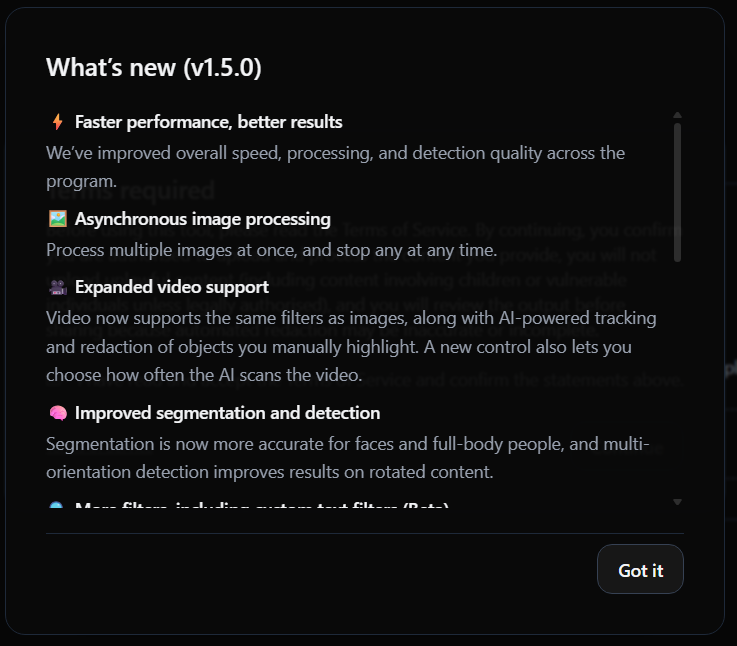
\includegraphics[width=\textwidth, trim=35 35 35 35, clip]{figures/images/chapter-6/PatchNotesExamples.png}
        \caption{Patch notes dialog summarizing user-visible system changes.}
        \label{fig:patch_notes}
    \end{subfigure}

    \caption{Supporting interface dialog for responsible use and system communication.}
    \label{fig:user_guidance_dialogs}
\end{figure}
\chapter{Technologies-and-Methodologies}
\label{chap:technologies_and_methodologies}

This chapter describes the technologies used to support SafeVision's processing of both still images and video, including frontend interaction, backend processing, machine learning integration, and deployment infrastructure.

\section{Frontend Technologies}

The frontend of the SafeVision system was developed as a web-based application using modern JavaScript technologies. The technology stack was selected to support interactive processing of both still images and video, efficient user workflows, and privacy-aware handling of sensitive data.

\methodheading{Core Frontend Framework}

The frontend is implemented using React in combination with TypeScript. React was chosen due to its component-based architecture \cite{react_components}, which enables modular and reusable user interface development by decomposing complex interfaces into smaller components. In addition, React’s rendering model is based on the concept of a virtual DOM \cite{react_virtual_dom}, which allows efficient updates by re-rendering only the parts of the interface that change \cite{virtual_dom_overview}, thereby improving performance in dynamic applications. This combination is particularly suitable for SafeVision, where interactive visualization of still images and video frames, together with real-time updates of detection results, requires efficient rendering and modular UI components.

TypeScript was used to introduce static typing to the codebase, providing improved reliability by catching errors during development \cite{typescript_benefits} and enhancing maintainability through clearer interfaces between components. This is particularly beneficial in larger systems where multiple modules interact and evolve over time.

To streamline the development workflow, Vite was selected as the build tool and development server \cite{vite}. Vite provides fast hot module replacement and efficient production builds through native ES module support, enabling rapid iteration during development and improved runtime performance in the deployed application.

In addition, React’s extensive ecosystem provides access to a wide range of third-party libraries and tools, supporting faster development and easier integration of additional functionality.

\methodheading{User Interface and Styling}

The user interface was implemented using modern CSS techniques, with Tailwind CSS as the primary styling framework. Tailwind CSS is a utility-first framework \cite{tailwind_css} that enables developers to construct user interfaces directly within component markup, reducing the need for separate CSS files and improving development efficiency. This approach allows rapid iteration and fine-grained control over styling \cite{utility_first_css}, which is particularly useful in interactive applications.

As illustrated in Figure~\ref{fig:tailwind_comparison}, Tailwind CSS differs from traditional CSS by applying utility classes directly within the markup rather than relying on separate style sheets. This reduces context switching during development and enables faster iteration when modifying user interface components. This is particularly beneficial in SafeVision, where interactive editing of detected regions requires rapid UI updates and precise control over visual elements. This approach also promotes consistency in styling by encouraging the reuse of predefined utility classes, reducing variability in design across components.

\begin{figure}[H]
\centering
\begin{minipage}{0.45\textwidth}
\textbf{Traditional CSS}
\begin{lstlisting}[language=HTML]
<button class="btn-primary">Continue</button>
\end{lstlisting}

\begin{lstlisting}
.btn-primary {
  height: 40px;
  padding: 0 16px;
  border-radius: 12px;
  font-size: 14px;
  font-weight: 500;
  border: 1px solid #374151;
  background-color: #111827;
  color: #f9fafb;
}
\end{lstlisting}
\end{minipage}
\hfill
\begin{minipage}{0.45\textwidth}
\textbf{Tailwind CSS}
\begin{lstlisting}[language=HTML]
<button class="h-10 px-4 rounded-xl text-sm 
font-medium border border-gray-700 
bg-neutral-900 text-gray-100 
hover:border-gray-400 transition">
  Continue
</button>
\end{lstlisting}
\end{minipage}

\caption{Comparison between traditional CSS and Tailwind CSS. The traditional approach separates styling into external stylesheets, while Tailwind CSS applies utility classes directly in the markup, enabling faster iteration and more localized styling.}
\label{fig:tailwind_comparison}
\end{figure}

The frontend was designed to support a human-in-the-loop workflow, where automated detection is combined with manual user control. Interactive interfaces play a key role in such systems \cite{human_in_loop_ai}, as they allow users to review and refine automated outputs. The interface therefore includes components for image visualization, control panels, and editing tools, enabling users to inspect detected regions and apply redaction methods while maintaining clarity and responsiveness, which are central usability principles \cite{usability_nielsen}.

The interface supports advanced user interactions such as zooming, panning, and direct manipulation of bounding boxes. These interactions are implemented using custom event handling and contribute to a more precise and efficient editing workflow, particularly when working with high-resolution images.

In addition to styling and layout, efficient rendering of visual elements is essential for interactive applications.

\methodheading{Canvas-Based Rendering}

The frontend utilizes HTML5 canvas-based rendering to support interactive visualization and manipulation of both still images and video frames. Canvas rendering enables efficient drawing and updating of graphical elements such as bounding boxes and overlays, which is essential for real-time interaction with detection results. Compared to standard DOM-based rendering, the canvas approach provides better performance for frequent graphical updates and fine-grained control over rendering behavior. This approach allows users to modify, resize, and reposition detected regions directly within the interface, supporting the human-in-the-loop workflow of the system. The same rendering approach is used to display overlays for video detections on individual frames, allowing consistent interaction patterns across image and video workflows.

\methodheading{State Management}

State management is handled using React’s built-in hooks and context mechanisms, enabling shared application state across components. Centralized state handling ensures consistent synchronization of updates throughout the interface \cite{react_state_management}. This is particularly important in SafeVision, where user interactions such as modifying bounding boxes, filtering detection results, or adjusting redaction settings require immediate and consistent updates across multiple UI components.

\begin{figure}[H]
\centering
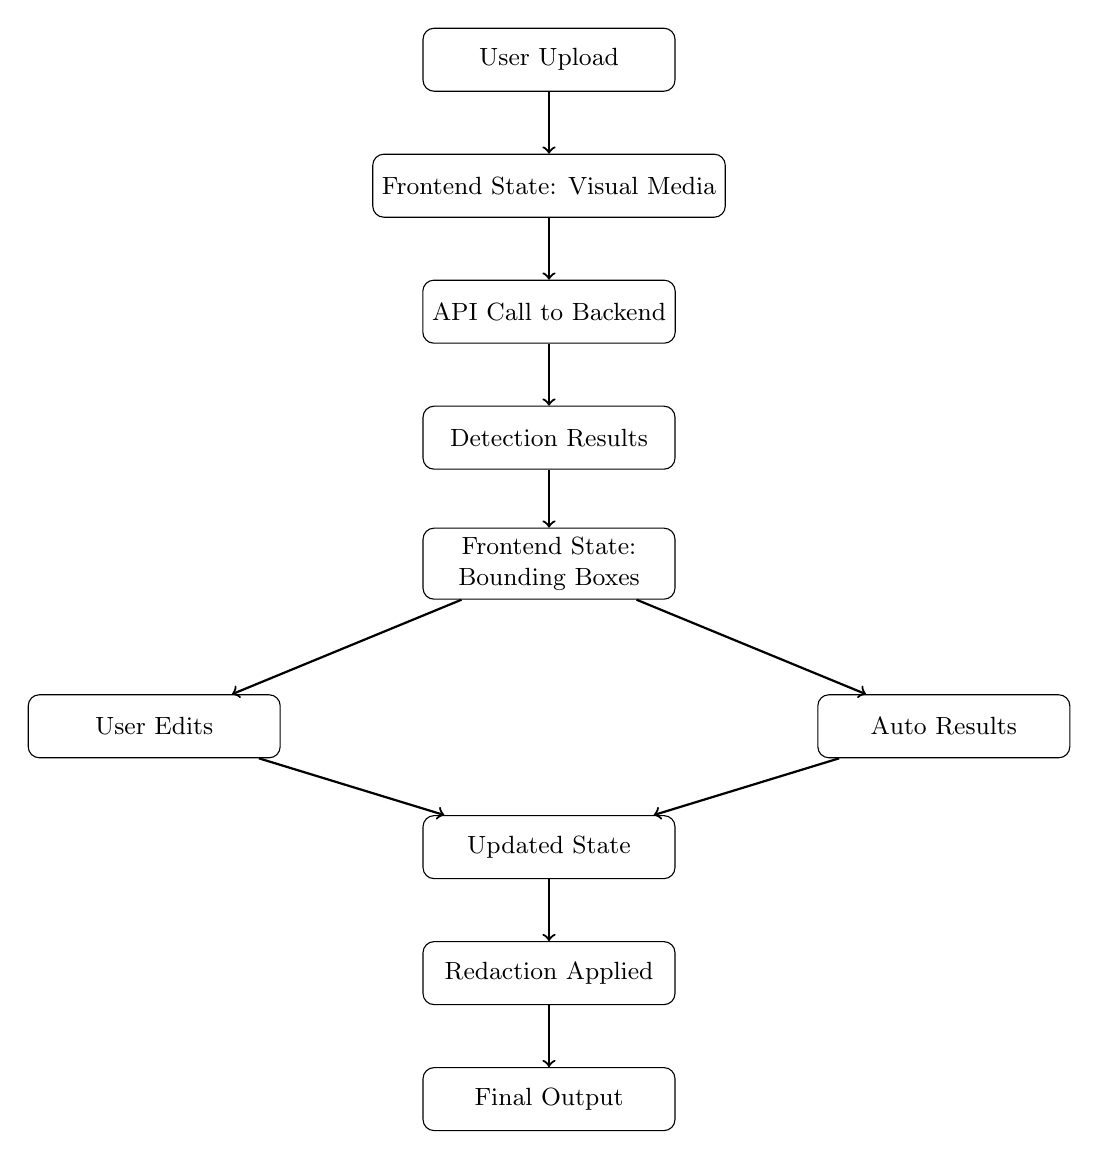
\begin{tikzpicture}[
    node distance=1.6cm,
    every node/.style={font=\small},
    state/.style={
        rectangle, 
        rounded corners, 
        draw=black, 
        minimum width=3.2cm, 
        minimum height=0.8cm, 
        align=center
    },
    arrow/.style={->, thick}
]

% Nodes
\node[state] (upload) {User Upload};
\node[state, below of=upload] (image) {Frontend State: Visual Media};
\node[state, below of=image] (api) {API Call to Backend};
\node[state, below of=api] (results) {Detection Results};
\node[state, below of=results] (boxes) {Frontend State:\\ Bounding Boxes};

\node[state, below left=1.2cm and 1.8cm of boxes] (edit) {User Edits};
\node[state, below right=1.2cm and 1.8cm of boxes] (auto) {Auto Results};

\node[state, below of=boxes, yshift=-2cm] (updated) {Updated State};
\node[state, below of=updated] (redact) {Redaction Applied};
\node[state, below of=redact] (output) {Final Output};

% Arrows (main flow)
\draw[arrow] (upload) -- (image);
\draw[arrow] (image) -- (api);
\draw[arrow] (api) -- (results);
\draw[arrow] (results) -- (boxes);

% Branches
\draw[arrow] (boxes) -- (edit);
\draw[arrow] (boxes) -- (auto);

% Merge
\draw[arrow] (edit) -- (updated);
\draw[arrow] (auto) -- (updated);

% Final flow
\draw[arrow] (updated) -- (redact);
\draw[arrow] (redact) -- (output);

\end{tikzpicture}

\caption{State management and data flow in the frontend application. The figure illustrates how visual media data and detection results are stored, updated, and transformed throughout the user workflow, including backend communication and user-driven modifications.}
\label{fig:state-management-flow}

\end{figure}

\methodheading{Client-Side Storage and Privacy Considerations}

To support privacy-by-design principles, the SafeVision frontend utilizes a combination of client-side storage mechanisms, primarily localStorage and IndexedDB. These technologies enable persistent storage of application data directly within the user’s browser, reducing the need to transmit sensitive information to external servers and aligning with data minimization principles defined in GDPR \cite{gdpr_reference}.

LocalStorage is used for lightweight configuration data, such as user preferences and interface settings. This includes information such as theme selection, UI layout configurations, and user consent status. These data elements are small in size and require simple key-value storage, making localStorage a suitable and efficient solution.

In contrast, IndexedDB is used for storing larger and more complex data structures, such as image annotations and video processing results. IndexedDB provides an asynchronous and structured storage model, allowing efficient handling of larger datasets without blocking the main application thread. This is particularly important in SafeVision, where annotation data may include multiple bounding boxes and metadata associated with high-resolution images and video frames.

Figure~\ref{fig:indexeddb_storage} illustrates the structure of client-side storage used in the application. The system maintains multiple logical databases and object stores to separate concerns such as image annotations and video-related data, improving maintainability and scalability.

\begin{figure}[H]
\centering
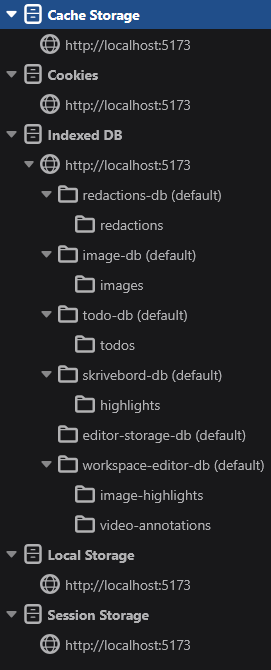
\includegraphics[height=0.4\textheight]{figures/images/chapter-7/storage-solution.png}
\caption{Overview of client-side storage in the application using IndexedDB.}
\label{fig:indexeddb_storage}
\end{figure}

As shown in Table~\ref{tab:storage_overview}, the storage design separates lightweight configuration data from larger annotation data. This distinction ensures efficient use of browser storage mechanisms while maintaining responsiveness and scalability in the application.

\begin{table}[H]
\centering
\begin{tabular}{|p{4cm}|p{3cm}|p{7cm}|}
\hline
\textbf{Storage Key / Store} & \textbf{Storage Type} & \textbf{Purpose} \\
\hline
workspace:consent:gdpr:v1 & localStorage & Stores whether the user has accepted the terms and conditions, ensuring compliance with GDPR requirements. \\
\hline
workspace:user-preferences:v1 & localStorage & Persists user interface preferences such as theme, highlight styles, and interaction settings across sessions. \\
\hline
workspace:sidebar:width & localStorage & Stores the current width of the sidebar to maintain a consistent layout between sessions. \\
\hline
workspace:patch-notes:seen-version & localStorage & Tracks which version of patch notes the user has already viewed to avoid repeated notifications. \\
\hline
image-highlights & IndexedDB & Stores bounding box annotations for images, including manually adjusted and automatically detected regions. \\
\hline
video-annotations & IndexedDB & Stores structured detection results for video frames, enabling persistence of annotations across sessions. \\
\hline
\end{tabular}
\caption{Overview of client-side storage keys and their purposes in the SafeVision frontend.}
\label{tab:storage_overview}
\end{table}

\methodheading{API Communication}

Communication between the frontend and backend is performed through HTTP-based API requests following REST principles. RESTful architectures \cite{rest_fielding} provide a standardized and scalable approach to communication between distributed systems, enabling a clear separation between client and server responsibilities. A structured service layer is used to manage these interactions, improving maintainability and the separation of concerns.

Together, these technologies provide a flexible and efficient foundation for developing an interactive, responsive, and privacy-aware frontend application.

\section{Backend Technologies and Languages}

The backend system was developed in Python, which was used for the computer vision components, the machine learning pipeline, and the FastAPI-based communication layer between the frontend and backend. This choice provided a consistent technology stack across the backend while also taking advantage of Python’s extensive library ecosystem for machine learning, image processing,
and frame-based video processing.

Machine learning components in the image redaction system follow a structured development pipeline consisting of data preparation, model training, and deployment. This process is applied to all detection models used in the system, including face detection, text detection, and QR/barcode detection.


\methodheading{FastAPI Application and API Structure}

The backend of SafeVision was implemented using FastAPI as the main application
framework. FastAPI was selected because it provides a lightweight and efficient
way to define REST-based APIs, while also supporting asynchronous request
handling. This made it well suited for a system that performs visual media processing and machine learning inference, where responsiveness and scalability are
important.

FastAPI also provides automatic request validation and clear endpoint
definitions, which simplified the implementation of the backend API and improved
maintainability during development.

Support for asynchronous execution was another important factor. Since detection
tasks may involve multiple independent models, the backend was designed to
support concurrent processing where possible. This contributes to better
responsiveness and improves the system’s ability to handle computationally
intensive tasks efficiently.


\methodheading{Backend Processing Utilities}

In addition to the FastAPI application layer, the backend relies on a set of
processing utilities that support image decoding, preprocessing, concurrent
execution, output normalization, and temporary file management. These utilities
were selected to make the backend pipeline more reusable and to reduce repeated
logic across detection and redaction endpoints.

For image handling, the backend uses OpenCV and NumPy to decode uploaded image
files into array representations suitable for inference and image processing.
This provides efficient low-level support for reading, transforming, and
encoding image data in the detection and redaction pipeline.

Model-specific preprocessing is handled through shared utility functions that
apply scaling, adaptive scaling, and optional preprocessing before inference.
This was important because the integrated detection models have different input
characteristics, and a shared preprocessing layer made it easier to support
multiple models without duplicating preparation logic across endpoints.

To improve responsiveness, the backend uses Python's \texttt{asyncio} utilities
to execute independent detection tasks concurrently where possible. This is
particularly relevant when multiple detectors are applied to the same image, as
it reduces waiting time compared with strictly sequential execution. At the same
time, synchronization mechanisms are used where necessary to avoid unsafe
concurrent access to shared processing resources in the redaction pipeline.

Another important utility layer concerns output normalization and validation.
Since the integrated models produce results in different formats, shared
processing logic is used to convert them into a unified representation before
they are returned through the API. This includes validation and adjustment of
bounding box coordinates to ensure that downstream components receive
well-formed results.

For video processing, the backend extends the same utility-based approach to frame-based media handling. OpenCV is used to open uploaded video files, read frames sequentially, access video properties such as frame rate and frame dimensions, and write temporary processed video output. This allows videos to be handled as sequences of image frames, while still relying on the same low-level image representation used by the rest of the backend.

The backend also uses FFmpeg as a final video-output utility. While OpenCV is
practical for writing processed frames during computation, FFmpeg is used
through the helper function \texttt{remux\_to\_h264\_aac(...)} to finalize the
processed video output and improve playback compatibility in browser and
media-player environments.

Because video processing involves larger files and intermediate outputs, the backend uses temporary file and directory handling based on Python’s standard file-management utilities. Uploaded videos, temporary processed files, and final outputs are isolated in request-specific working directories and cleaned up after detection or redaction has completed.

Table~\ref{tab:backend_processing_utilities} summarizes the main backend
processing utilities and their technical roles in the system.

\begin{table}[H]
\centering
\renewcommand{\arraystretch}{1.5}
\begin{tabular}{p{3.2cm} p{3.5cm} p{7cm}}
\toprule
\textbf{Utility area} & \textbf{Technology} & \textbf{Purpose} \\
\midrule
Image and video decoding and processing & \texttt{OpenCV}, \texttt{NumPy} & Decode uploaded image files and video frames, convert visual data into array representations, and support low-level processing in detection and redaction workflows. \\

Video output finalization & \texttt{FFmpeg} & Finalize processed video files through \texttt{remux\_to\_h264\_aac(...)} to improve playback compatibility across clients. \\

Preprocessing support & Shared preprocessing utilities & Apply scaling, adaptive resizing, and optional preprocessing before inference for different detection models. \\

Concurrent execution & Python \texttt{asyncio} & Run independent detection tasks concurrently to improve backend responsiveness. \\

Synchronization & Python \texttt{asyncio.Lock} & Prevent unsafe concurrent execution in shared parts of the redaction pipeline. \\

Output normalization & Shared normalization logic & Convert heterogeneous model outputs into a unified response format for frontend integration and downstream processing. \\

Temporary workspace handling & \texttt{tempfile}, \texttt{pathlib}, \texttt{shutil} & Manage request-specific temporary files and directories for video upload, intermediate processing, output generation, and cleanup. \\
\bottomrule
\end{tabular}
\caption{Overview of backend processing utilities used in the SafeVision backend.}
\label{tab:backend_processing_utilities}
\end{table}



\section{Machine Learning Technologies and Development Environment}

SafeVision relies on a separate machine learning development environment for
dataset preparation, model training, and evaluation of custom models. This
environment was maintained in a dedicated repository, while the deployed
SafeVision application was implemented in a separate repository focused on
inference, redaction, API handling, and frontend interaction.

\begin{figure}[H]
\centering
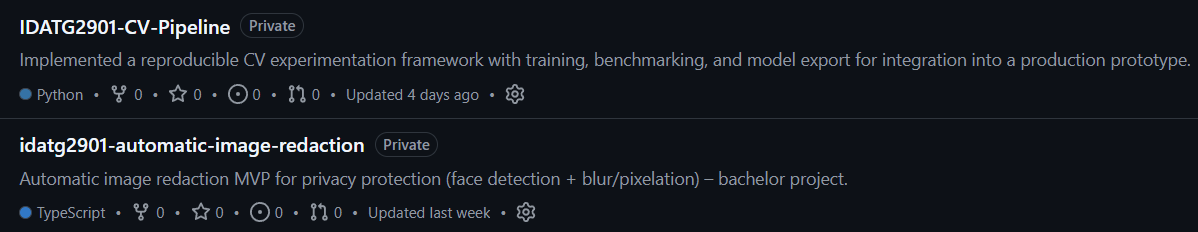
\includegraphics[width=1.0\textwidth]{figures/images/chapter-8/cv_repos.png}
\caption{Separation between the machine learning development repository and the
SafeVision application repository. The development repository was used for
dataset preparation, training, and evaluation, while the SafeVision repository
contains the deployed inference and redaction system.}
\label{fig:cv_repos}
\end{figure}

This separation was motivated not only by workflow considerations, but also by
technical differences between the two environments. Model development required
heavier machine learning dependencies, dataset-processing scripts, training
utilities, and evaluation workflows that were not needed in the deployed
application. Keeping these concerns separate reduced dependency conflicts and
made it easier to manage different library versions, requirements files, and
virtual environments for training and deployment.

The machine learning environment was used for the development of the custom
YOLOX-based object detection models for barcode and license plate detection, as
well as the text analysis components used for selective text redaction. In the case 
of text processing, this included a fine-tuned named entity recognition model adapted 
for Norwegian and English text. These components required a different development
setup from the production backend, where the main goal was stable inference rather
than iterative experimentation.

\begin{figure}[H]
\centering
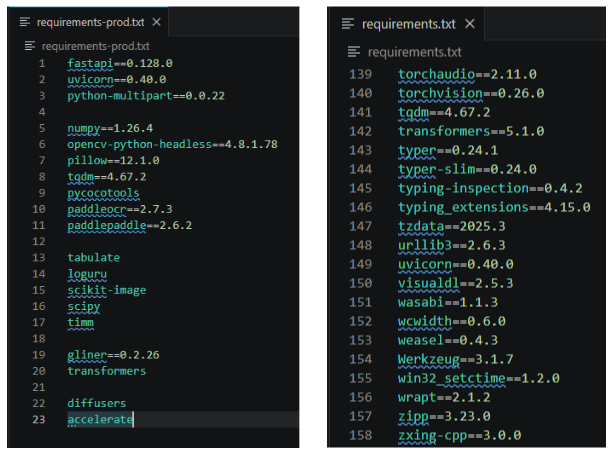
\includegraphics[width=0.7\textwidth]{figures/images/chapter-7/requirements.png}
\caption{Excerpts from \texttt{requirements.txt} and \texttt{requirements-prod.txt}, 
showing the difference in dependency set size.} 
\label{fig:requirements_comparison}
\end{figure}

The specific training, preprocessing, and integration steps are described in
Chapter~\ref{chap:implementation_details}. The present section instead focuses
on the technological and environmental choices that supported machine learning
development across the two repositories.

\section{Deployment and Infrastructure}

The project relied on a small set of deployment and infrastructure technologies
to support delivery, automation, and collaboration. Docker was used for
containerization, GitHub Actions for CI/CD automation, Google Cloud for hosting
and deployment, and GitHub for version control and team collaboration.

\begin{table}[H]
\centering
\begin{tabular}{p{3.2cm} p{4cm} p{6.5cm}}
\toprule
\textbf{Technology} & \textbf{Role} & \textbf{Purpose in the project} \\
\midrule
Docker & Containerization & Package the backend and its dependencies into a consistent runtime environment. \\

GitHub Actions & CI/CD automation & Automate validation, build, and deployment workflows. \\

Google Cloud & Cloud platform & Host and deploy the backend and frontend application components. \\

GitHub & Version control and collaboration & Support branch-based development, code sharing, and team coordination. \\
\bottomrule
\end{tabular}
\caption{Deployment and infrastructure technologies used in the project.}
\label{tab:deployment_infrastructure_tech}
\end{table}

Docker was used to package the backend application and its dependencies into a
consistent runtime environment. This reduced environment-specific issues and
simplified deployment across development and production stages.

GitHub was used for version control, code sharing, and collaboration throughout
the project. This supported branch-based development, change tracking, and team
coordination. In addition, GitHub Actions was used to implement CI/CD. The CI
workflow was used to validate changes through automated checks, while the CD
workflow was used to build and deploy updated application artifacts.

Google Cloud was used as the deployment platform for the SafeVision system. It
provided the cloud environment used to host the deployed application
components.

\chapter{Implementation Details}
\label{chap:implementation_details}

This chapter describes how the \gls{SafeVision} system was implemented in practice. It explains the frontend and backend implementation, the development of custom \acrshort{ml} models, the integration of \acrshort{ml} components, and the image and video processing pipelines used for detection and redaction. The chapter also presents the deployment setup, including continuous integration, continuous deployment, containerization, and environment configuration.

\section{Frontend Implementation}

The frontend provides an interactive environment for uploading images, visualizing detection results, adjusting detected regions, and applying redaction. The implementation emphasizes modularity, responsiveness, and user control, in line with the system’s hybrid workflow.

\methodheading{Architecture and Structure}

This section builds on the overall system architecture described in Chapter~5 by explaining how the frontend was implemented in the codebase. The frontend follows a feature based modular architecture, where the codebase is organized into domain-specific modules such as \texttt{detection}, \texttt{workspace}, \texttt{file}, and \texttt{userPreference}. Each module is structured as a self contained unit consisting of React components, custom hooks, state management logic, and supporting utilities.

This organization is illustrated in Figure~\ref{fig:frontend_structure}, where the frontend is divided into feature modules supported by shared UI, service, and storage layers. For example, the \texttt{detection} module contains components for filtering, such as \texttt{DetectionFiltersSection}, domain logic for mapping and grouping detections, and state stores for managing filter selections. Similarly, the \texttt{workspace} module includes canvas-related components, such as \texttt{CanvasSurface} and \texttt{PageEditorSurface}, as well as hooks for interaction logic, including \texttt{useHighlightBoxEditor}, \texttt{useImageRedaction}, and \texttt{useImageEditor}.

\begin{figure}[H]
\centering
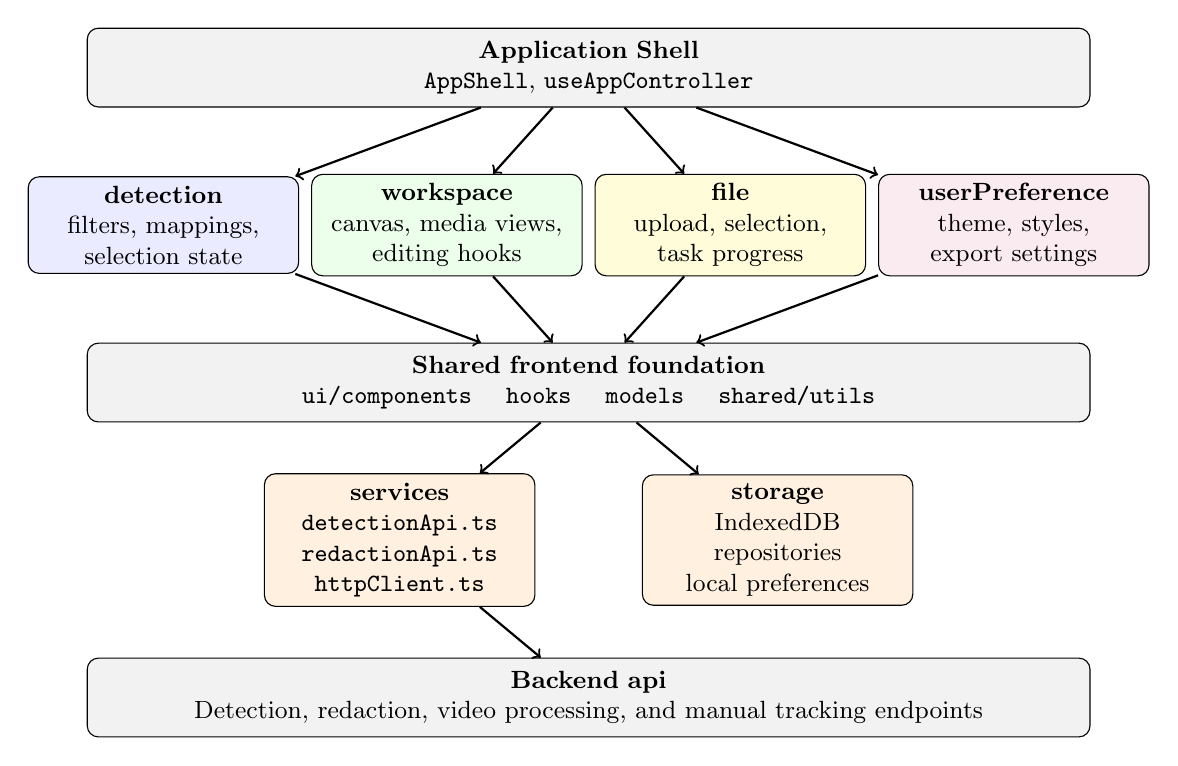
\begin{tikzpicture}[
    every node/.style={font=\small},
    box/.style={
        rectangle,
        rounded corners,
        draw=black,
        align=center,
        minimum height=1cm,
        text width=3.2cm
    },
    widebox/.style={
        rectangle,
        rounded corners,
        draw=black,
        align=center,
        minimum height=1cm,
        text width=12.5cm
    },
    arrow/.style={->, thick}
]

% Top level
\node[widebox, fill=gray!10] (app) at (0, 4)
{\textbf{Application Shell}\\
\texttt{AppShell}, \texttt{useAppController}};

% Feature modules
\node[box, fill=blue!8] (detection) at (-5.4, 2)
{\textbf{detection}\\
filters, mappings,\\
selection state};

\node[box, fill=green!8] (workspace) at (-1.8, 2)
{\textbf{workspace}\\
canvas, media views,\\
editing hooks};

\node[box, fill=yellow!15] (file) at (1.8, 2)
{\textbf{file}\\
upload, selection,\\
task progress};

\node[box, fill=purple!8] (prefs) at (5.4, 2)
{\textbf{userPreference}\\
theme, styles,\\
export settings};

% Shared layer
\node[widebox, fill=gray!10] (shared) at (0, 0)
{\textbf{Shared frontend foundation}\\
\texttt{ui/components} \quad \texttt{hooks} \quad \texttt{models} \quad \texttt{shared/utils}};

% Service and storage layer
\node[box, fill=orange!12] (services) at (-2.4, -2)
{\textbf{services}\\
\texttt{detectionApi.ts}\\
\texttt{redactionApi.ts}\\
\texttt{httpClient.ts}};

\node[box, fill=orange!12] (storage) at (2.4, -2)
{\textbf{storage}\\
IndexedDB repositories\\
local preferences};

% Backend
\node[widebox, fill=gray!10] (backend) at (0, -4)
{\textbf{Backend \acrshort{api}}\\
Detection, redaction, video processing, and manual tracking endpoints};

% Arrows
\draw[arrow] (app) -- (detection);
\draw[arrow] (app) -- (workspace);
\draw[arrow] (app) -- (file);
\draw[arrow] (app) -- (prefs);

\draw[arrow] (detection) -- (shared);
\draw[arrow] (workspace) -- (shared);
\draw[arrow] (file) -- (shared);
\draw[arrow] (prefs) -- (shared);

\draw[arrow] (shared) -- (services);
\draw[arrow] (shared) -- (storage);
\draw[arrow] (services) -- (backend);

\end{tikzpicture}

\caption{Feature-based frontend structure in \gls{SafeVision}. Domain-specific modules encapsulate their own components, hooks, state logic, and utilities, while shared UI elements, services, and storage repositories are reused across the application.}
\label{fig:frontend_structure}
\end{figure}

Shared functionality is implemented through a dedicated service layer located in the \texttt{services} directory. This includes modules such as \texttt{detectionApi.ts} and \texttt{redactionApi.ts}, which handle communication with the backend, as well as a centralized HTTP client, \texttt{httpClient.ts}, for managing requests. This ensures that networking logic is decoupled from UI components.

This structure realizes the separation of concerns described in Chapter~\ref{user_interface_and_usability} by keeping feature-specific logic separated from shared UI components, service communication, and storage mechanisms. As a result, the frontend can be maintained and extended without requiring changes across unrelated parts of the codebase.

\methodheading{State Management and Interaction Logic}

State management is implemented using custom React hooks and centralized stores. Hooks such as \texttt{useDetectionsStore}, \texttt{useHighlightsStore}, and \texttt{useImages} manage application state related to detection results, annotations, and uploaded files.

\begin{lstlisting}[language=javascript, caption={Per-file detection state managed through a custom hook}, label={lst:frontend_detection_store}]
type DetectionsStore = Record<string, Rect[]>;

export function useDetectionsStore(): DetectionsStoreApi {
  const [storeByFileKey, setStoreByFileKey] = useState<DetectionsStore>({});

  const get = useCallback(
    (fileKey: string | null) => {
      if (!fileKey) return [];
      return storeByFileKey[fileKey] ?? [];
    },
    [storeByFileKey],
  );

  const set = useCallback((fileKey: string, rects: Rect[]) => {
    setStoreByFileKey((prev) => ({ ...prev, [fileKey]: rects }));
  }, []);

  return { get, set, reset, dump, restore };
}
\end{lstlisting}

Listing~\ref{lst:frontend_detection_store} shows how detection results are stored per file key. This makes it possible to switch between uploaded media while keeping each file's detections separate. The state is updated immutably, which fits React's rendering model and makes the store compatible with undo and redo snapshots.

Since detection and highlight state are stored centrally, updates made in the workspace can be reflected immediately in related interface elements, such as filters, redaction controls, and preview components. For example, when a user modifies a \gls{bounding box} in the workspace, the updated region is available to the rest of the interface without requiring the user to manually reload or reprocess the image.

The system also includes undo and redo functionality through history-aware hooks, such as \texttt{useUndoRedoHistory}. This allows users to safely experiment with edits without losing previous states, which is particularly important in a workflow where users may need to manually correct automatically detected regions.

\methodheading{Workspace and Image Interaction}

A central part of the frontend is the workspace system, which provides an interactive canvas for image manipulation. Components such as \texttt{CanvasSurface}, \texttt{PageEditorSurface}, and \texttt{ImageWorkspace} enable rendering of images and overlaying of detection results, as illustrated earlier in Figure~\ref{fig:ui_final_examples}.

Detected regions are represented as \gls{bounding box}es, which can be selected, resized, moved, or deleted by the user. Interaction logic is handled through hooks such as \texttt{useHighlightBoxEditor} and \texttt{useImageBoxes}, which manage user input and coordinate transformations. Separating this logic into hooks prevents the canvas components from becoming responsible for both rendering and interaction state. This is important because editing operations all depend on consistent coordinate handling between the displayed image and the original media dimensions.

The system also supports zooming, panning, and precise editing through custom hooks, such as \texttt{useZoom} and \texttt{useCtrlDragPan}. These mechanisms improve usability when working with high-resolution images, where sensitive regions may be small or difficult to adjust at the default zoom level.

\methodheading{Detection Integration in the UI}

Detection results are integrated into the frontend through a dedicated service layer, primarily through \texttt{detectionApi.ts}. When a user uploads an image and starts detection, the image is sent to the backend, and the returned detections are stored in the detection state.

\begin{lstlisting}[language=javascript, caption={Frontend detection request through the service layer}, label={lst:frontend_detection_request}]
export async function detectObjects(
  file: Blob,
  mode: DetectMode = "all",
  scale: number = 1,
  adaptiveScaling?: boolean,
  multiOrientation?: boolean,
  usePreprocess: boolean = false,
  signal?: AbortSignal,
): Promise<DetectResponse> {
  if (file.size === 0) {
    throw new Error("No file uploaded");
  }

  if (scale <= 0 || scale > 4) {
    throw new Error("Scale must be between 0 and 4");
  }

  const formData = new FormData();
  formData.append("file", file, "image.png");

  return postForm<DetectResponse>("/detect", {
    formData,
    query: {
      types: mode,
      ...(adaptiveScaling ? { adaptive_scaling: true } : { scale: scale ?? 1 }),
      use_preprocess: usePreprocess,
      ...(multiOrientation ? { multi_orientation: true } : {}),
    },
    signal,
    parseAs: "json",
  });
}
\end{lstlisting}

Listing~\ref{lst:frontend_detection_request} shows how detection requests are isolated in the service layer. UI components do not construct HTTP requests directly; instead, they call a typed service function that validates the input, builds the multipart request payload, forwards detection options as query parameters, and returns a structured detection response.

The UI provides filtering and categorization tools, such as \texttt{DetectionFiltersSection} and \texttt{CategoryMultiSelect}, which allow users to control which types of detections are visible. This is important when multiple detection models are used, as it helps reduce visual clutter and makes it easier for users to review the categories of sensitive information that are relevant to the current task.

\methodheading{Redaction Workflow Implementation}

The redaction workflow is implemented through hooks such as \texttt{useImageRedaction} and \texttt{useWorkspaceRedaction}, which coordinate the transformation of selected regions. Users can apply redaction either based on detected regions, or manually by defining custom areas. Redaction parameters, such as blur or pixelation, are controlled through UI components in the sidebar.

Before redaction is sent to the backend, the frontend filters out disabled regions and converts the remaining \gls{bounding box}es from canvas coordinates back to original image coordinates. This conversion is necessary because the user edits boxes on a scaled canvas, while the backend must redact the original image data.

\begin{lstlisting}[language=javascript, caption={Preparing selected regions for image redaction}, label={lst:frontend_redaction_workflow}]
async function redact() {
  // Only user-approved regions are sent to the backend.
  const activeRects = visibleHighlights.filter(
    (r) => r.enabled !== false,
  );

  if (!activeRects.length || !imgEl || !canvasRef.current) {
    return;
  }

  const rectsOriginal = activeRects.map((r) => {
    // Convert from displayed canvas coordinates to original image coordinates.
    const transformed = canvasRectToOriginal({
      rect: r,
      canvas: canvasRef.current,
      imgEl,
    });

    return {
      ...r,
      ...transformed,
    };
  });

  await redactBackend(rectsOriginal);

  // Clear stale boxes after the image has been redacted.
  hl.reset();
  detectionsStore.reset(fileKey);
}
\end{lstlisting}

Listing~\ref{lst:frontend_redaction_workflow} shows how the frontend prepares redaction input after the user has reviewed the detected or manually added regions. Only enabled regions are included, and each region is transformed to match the original media dimensions before being sent to the backend. After a successful redaction, local highlights and detection results are cleared so that outdated \gls{bounding box}es are not shown on top of the newly redacted image.

The frontend ensures that redaction is applied only to the active regions selected or approved through the user workflow. This maintains user control and reduces the risk of unintended modifications. The final result can then be exported using utilities such as \texttt{canvasExporter.ts}, which prepares the redacted media for download. During this export process, image metadata is not preserved in the downloaded output, as discussed in Appendix~\ref{appsec:relevant_metadata_categories}. This occurs automatically as a result of the canvas-based export workflow, without requiring a separate metadata-stripping implementation.


\methodheading{File Handling and User Workflow}

File management is handled through the \texttt{file} module, which includes components such as \texttt{FilePanel} and \texttt{UploadDropzone}. Users can upload, organize, and switch between multiple images within the same session.

Custom hooks, such as \texttt{useFileUpload} and \texttt{useFileSelection}, manage file operations. This supports workflows where several files are processed in one session and provides visual feedback during longer running operations. By keeping file handling separate from detection and redaction logic, the frontend avoids coupling media management directly to processing functionality, making it easier to support future extensions such as additional file types, improved batch handling, or alternative upload mechanisms.

\methodheading{Client-Side Storage and Privacy Considerations}

To support privacy oriented data handling, the frontend uses client side storage mechanisms for preferences, workflow state, and annotation data. Annotation data such as image highlights is stored through IndexedDB repositories such as \texttt{highlightsIndexedDbRepository}, while user preferences are stored separately through the user preferences repository and browser local storage. This keeps these data types local to the browser rather than persistently storing them on the server. This supports the project’s data minimization strategy by limiting unnecessary server-side persistence and allows users to continue working with locally stored annotation data during a session without requiring all interaction state to be maintained by the backend.

\begin{lstlisting}[language=javascript, caption={Fail-safe IndexedDB persistence for highlights}, label={lst:indexeddb_highlights}]
async save(key: string, rects: Rect[]): Promise<void> {
  try {
    const dbp = getEditorDb();

    // In test mode or unsupported browsers, persistence is skipped safely.
    if (!dbp) return;

    const db = await dbp;
    await db.put(EDITOR_STORE_NAMES.imageHighlights, {
      fileKey: key,
      rects,
      updatedAt: Date.now(),
    });
  } catch (err) {
    // Storage failure should not block the editing workflow.
    console.warn("IndexedDB save failed:", err);
  }
}
\end{lstlisting}

Listing~\ref{lst:indexeddb_highlights} shows the fail-safe storage pattern used for client-side annotation persistence. If IndexedDB is unavailable or the write operation fails, the error is handled locally instead of interrupting the user workflow. This supports privacy-oriented data handling by keeping annotation data in the browser, while also allowing the application to degrade gracefully if local storage is unavailable.

\section{Backend Implementation}
\label{backend_implementation}

The backend of Safe Vision is implemented as a layered architecture consisting of an \acrshort{api} layer and a computation backend. While the overall architecture was introduced in Chapter~7, this section explains how the design is realized in the codebase. Controllers, services, and pipeline components are organized into separate modules, allowing request handling, application logic, and \acrshort{ml} processing to remain decoupled.

\methodheading{API Layer}

The \acrshort{api} layer handles requests from the frontend and acts as the main entry point to the backend. The application uses modular routing, with separate controllers for different processing tasks. Listing~\ref{lst:fastapi_routing} shows how middleware and routes are registered in the application.

\begin{lstlisting}[caption={FastAPI application structure and routing}, label={lst:fastapi_routing}]
app = FastAPI(
    title="Automatic Image Redaction API",
    lifespan=lifespan
)

app.add_middleware(
    CORSMiddleware,
    allow_origins=ALLOWED_ORIGINS,
    allow_credentials=True,
    allow_methods=["*"],
    allow_headers=["*"],
)

app.include_router(detect_router, prefix="/api", tags=["Detection"])
app.include_router(redact_router, prefix="/api", tags=["Redaction"])
app.include_router(video_detect_router, prefix="/api", tags=["Video"])
app.include_router(video_redact_router, prefix="/api", tags=["Video"])
\end{lstlisting}

\begin{lstlisting}[caption={Detection endpoint with parallel execution}, label={lst:detect_endpoint}]
@router.post("/detect")
async def detect(file: UploadFile, types: str = Query(default="face")):
    data = await file.read()
    img_array = np.frombuffer(data, np.uint8)
    img = cv2.imdecode(img_array, cv2.IMREAD_COLOR)

    tasks = []

    # Run selected detectors in worker threads to avoid blocking the API handler.
    if "face" in types:
        face_detector = get_face_detector()
        tasks.append(asyncio.to_thread(run_pipeline_on_image, img, face_detector))

    if "text" in types:
        text_engine = get_text_ocr()
        tasks.append(asyncio.to_thread(run_pipeline_on_image, img, text_engine))

    # Aggregate all selected detector outputs into one response.
    results = await asyncio.gather(*tasks)

    return {"live": results}
\end{lstlisting}

The endpoint implementation keeps request handling separate from the computational parts of the backend. Listing~\ref{lst:detect_endpoint} shows how selected detection tasks are dispatched concurrently and aggregated into a single response, reducing latency when multiple detection types are requested in the same call. For redaction requests, the same layer receives image data together with detection results, validates the input, and forwards it to the processing pipeline where the selected redaction configuration is applied.


\methodheading{Computation Backend}

The computation backend performs the core processing tasks of the system, including detection and redaction of sensitive information. Unlike the \acrshort{api} layer, it is responsible for image processing and \acrshort{ml} \gls{inference} rather than request handling. It is organized into two main components: the detection pipeline and the redaction processing module.

\subsubsection{Detection Pipeline}

The detection pipeline analyzes visual media and identifies sensitive entities such as faces, text, \gls{barcode}s, license plates, and objects. It supports multiple task-specific detectors within a shared processing flow.

Once uploaded, the image is processed through a sequence of steps that prepares the input, runs the selected models, and converts the outputs into a shared result format for later review and redaction. Processing begins with optional preprocessing, where the input image may be scaled or enhanced to improve detection performance, particularly for small or low-quality inputs. The preprocessed image is then passed to one or more task-specific detection models. When multiple detectors are selected, they can be executed concurrently to improve throughput. The outputs are subsequently aggregated and converted into a shared representation that standardizes bounding-box coordinates, confidence scores, and entity labels.

\begin{lstlisting}[caption={Detection pipeline processing and bounding box normalization}, label={lst:run_pipeline}]
def run_pipeline_on_image(img_proc, detector, *, total_scale=1.0):
    detections = detector.detect(img_proc) or []

    boxes_xyxy = []
    scores = []

    # Reverse the preprocessing scale so boxes match the original image.
    inv_scale = 1.0 / total_scale if total_scale != 0 else 1.0

    for d in detections:
        x1 = int(round(d.x1 * inv_scale))
        y1 = int(round(d.y1 * inv_scale))
        x2 = int(round(d.x2 * inv_scale))
        y2 = int(round(d.y2 * inv_scale))

        boxes_xyxy.append((x1, y1, x2, y2))
        scores.append(float(d.score))

    return boxes_xyxy, scores
\end{lstlisting}

Listing~\ref{lst:run_pipeline} shows how detections are converted into a normalized \gls{bounding box} representation. The detector output is first collected as coordinate pairs and confidence scores, before the coordinates are rescaled back to the original image dimensions using the inverse of the preprocessing scale. This ensures that detection results remain consistent with the original media, even when preprocessing has resized the image before \gls{inference}. The final output of the detection pipeline is a structured representation of the detected entities, which is returned to the \acrshort{api} layer for further processing or visualization in the frontend.

\subsubsection{Redaction Processing}

The redaction processing module anonymizes sensitive image regions based on the output of the detection pipeline. It applies \gls{masking} and transformation methods to the identified areas. It receives the original image together with the detected regions and prepares these inputs for redaction. Depending on the selected configuration, the system applies either \gls{bounding box} \gls{masking} or \gls{segmentation} based \gls{masking}. When \gls{segmentation} is enabled, \gls{mobilesam} is used to generate more precise masks for complex shapes, as illustrated in Figure~\ref{fig:segmentation_comparison} in Chapter~\ref{chap:results}.

Once the \gls{masking} regions have been defined, the selected \gls{anonymization} method is applied. Each supporting redaction method representing a different trade-off between privacy, visual quality, and computational cost. Listing~\ref{lst:redaction_method} shows how the available \gls{anonymization} methods are applied through a shared interface. After processing, the image may be resized and encoded into a standard output format before being returned to the \acrshort{api} layer. This supports compatibility with the frontend and efficient data transfer.

\begin{lstlisting}[caption={Application of redaction methods}, label={lst:redaction_method}]
def _apply_method(method, out, roi, mask, pixel_size, inpaint_radius, box_coords=None):
    if method == "blur":
        _apply_blur(roi, mask)
    elif method == "pixelate":
        _apply_pixelate(roi, mask, pixel_size)
    elif method == "blackbox":
        _apply_blackbox(roi, mask)
    elif method == "inpaint":
        _apply_inpaint_full_image(out, box_coords, mask)
    else:
        raise ValueError(method)
\end{lstlisting}






\section{\acrshort{ml} Model Development}

This section describes the development of the custom \acrshort{ml} models used in \gls{SafeVision} before their integration into the application backend. The main development effort concerned two image-based \gls{object detection} models for barcodes and license plates, while a separate \acrshort{ner} pipeline was developed to identify sensitive textual entities in \acrshort{ocr}-extracted text. Since these tasks required different training data, preprocessing steps, and evaluation methods, the code, scripts, and training workflows were kept in separate \acrshort{ml} development repositories rather than in the deployed \gls{SafeVision} application repository (Figure~\ref{fig:cv_repos}). This separation made it possible to isolate preprocessing, training, experimentation, and evaluation from the production application, while allowing the deployed system to remain focused on \gls{inference} and system integration.

\methodheading{Overview of Training Pipeline}

The training pipeline described in this section applies to both the \gls{barcode} and license plate detection models. For clarity, the \gls{barcode} and QR detection pipeline is used as the primary example, while the same overall process was also applied to the license plate model.

\begin{figure}[H]
\centering
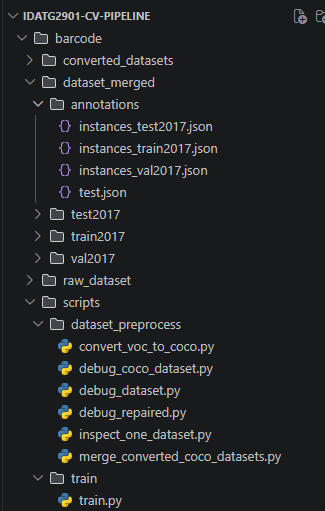
\includegraphics[width=\textwidth,height=0.40\textheight,keepaspectratio]{figures/images/chapter-8/cv_pipeline_structure.png}
\caption{Directory structure of the computer vision repository used for dataset preprocessing and model training.}
\label{fig:cv_pipeline_structure}
\end{figure}

The CV-repository, was structured to separate preprocessing, dataset management, and training into independent modules. This organization simplified experimentation and made it possible to reuse preprocessing steps across multiple training runs. The dataset followed a COCO-style structure with dedicated training, validation, and test splits together with corresponding annotation files. Preprocessing was handled by scripts in the \texttt{dataset\_preprocess} module, while model training was executed through the \texttt{train.py} entry point.

\methodheading{Dataset Preparation}

The dataset preparation process consisted of collecting multiple datasets from different sources, converting them into a unified annotation format, and merging them into a single dataset for training the \gls{barcode} detection model. Since few datasets were directly designed for \gls{barcode} and QR code detection, multiple sources were combined to construct a unified dataset (Table~\ref{tab:barcode_datasets}). Many existing datasets are intended for recognition rather than detection, which meant that several images either lacked suitable \gls{bounding box} annotations or required conversion to a detection format.

\begin{table}[H]
\centering
\begin{tabular}{|p{3.5cm}|p{3cm}|p{7.2cm}|}
\hline
\textbf{Dataset} & \textbf{Source} & \textbf{Description} \\ \hline

\textbf{archive\_1} & 
Kaggle \cite{barcode_qr_kaggle} & 
Collection of real-world \gls{barcode} and QR code images from diverse environments. \\ \hline

\textbf{\gls{barcode}\_bb, e8\_bb, multi\_bb} & 
Zenodo \cite{zenodo_barcode_datasets} & 
Benchmark datasets with \gls{bounding box} annotations for \gls{barcode} detection, including multiple instances per image. \\ \hline

\textbf{kaggle (InventBar, ParcelBar)} & 
Kaggle \cite{benchmark_barcode_kaggle} & 
Benchmark datasets containing \gls{barcode} images captured in industrial and logistics scenarios. \\ \hline

\textbf{syn10k\_plus\_huawei} & 
University of Szeged \cite{syn10k_dataset} & 
Synthetic \gls{barcode} dataset designed to increase data diversity and improve generalization. \\ \hline

\textbf{Total} & 
15731 & 
Combined into a unified dataset for training and evaluation. \\ \hline

\end{tabular}
\caption{Overview of datasets used for training the \gls{barcode} detection model.}
\label{tab:barcode_datasets}
\end{table}

In addition, most available datasets emphasize standard 1D \gls{barcode}s and QR codes, with more limited coverage of less common \gls{barcode} types. As a result, dataset preparation required substantial preprocessing, including annotation conversion, filtering, and merging of heterogeneous sources.

\begin{figure}[H]
\centering
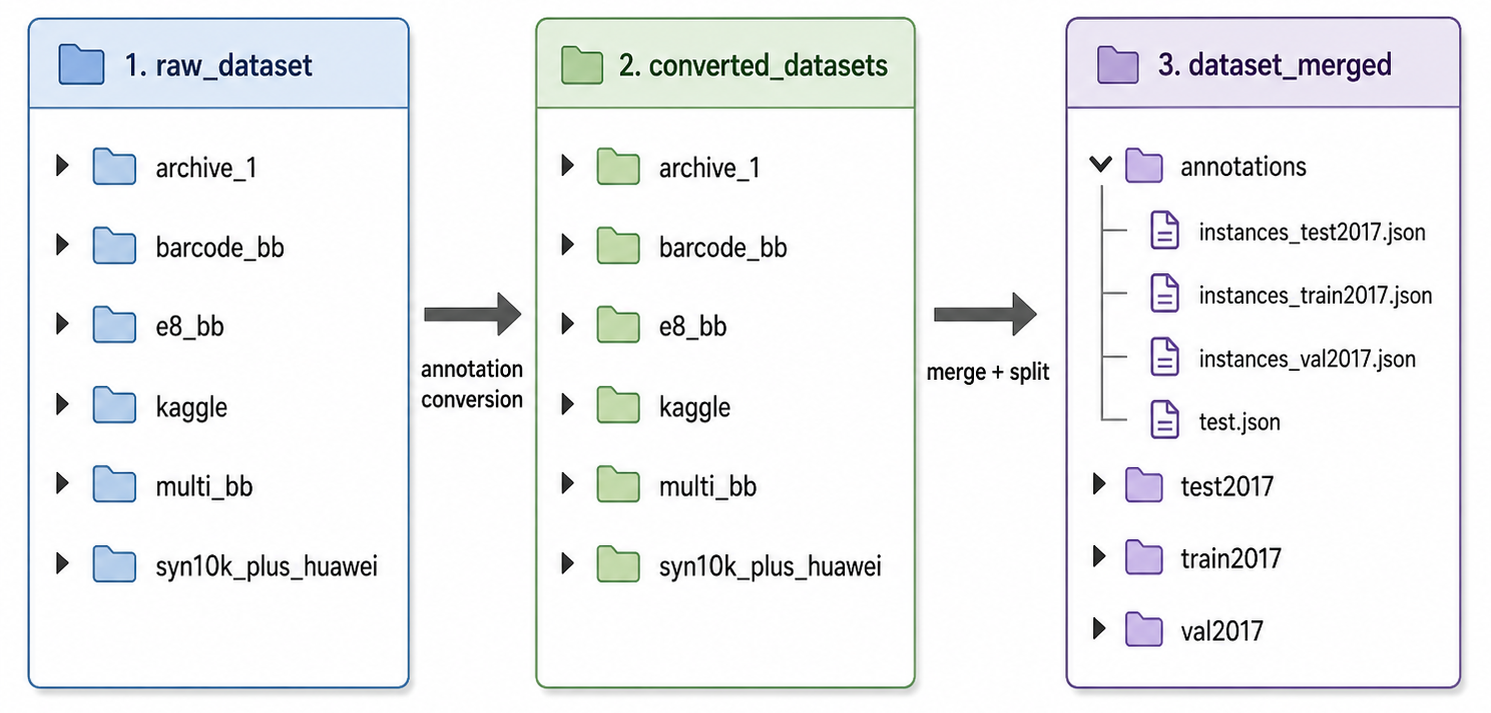
\includegraphics[width=\textwidth,height=0.25\textheight,keepaspectratio]{figures/images/chapter-8/dataset_preperation_pipeline.png}
\caption{Dataset preparation pipeline illustrating the transformation from raw datasets to a unified, merged, and split dataset used for training. Created by the au-
thors, with AI-assisted refinement}
\label{fig:dataset_preperation_pipeline}
\end{figure}

To ensure consistency across all data sources, each dataset was first converted into a unified annotation format. The datasets were then merged and divided into training, validation, and test subsets. As illustrated in Figure~\ref{fig:dataset_preperation_pipeline}, this process transformed raw datasets into a structured dataset suitable for training \gls{object detection} models. To maintain balanced source representation, the split was performed per dataset before the subsets were merged. This prevented larger datasets from dominating the final train, validation, and test distributions. Listing~\ref{lst:dataset_merge_split} shows the core splitting strategy used in the preprocessing script.

\begin{lstlisting}[caption={Per-dataset splitting strategy used during dataset merging}, label={lst:dataset_merge_split}]
def split_images_by_dataset(all_items):
    by_dataset = defaultdict(list)

    for item in all_items:
        by_dataset[item["dataset_name"]].append(item)

    train_items, val_items, test_items = [], [], []
    rng = random.Random(RANDOM_SEED)

    for dataset_name, items in by_dataset.items():
        # Shuffle each source separately so every dataset contributes to each split.
        rng.shuffle(items)

        n = len(items)
        n_train = int(n * TRAIN_RATIO)
        n_val = int(n * VAL_RATIO)

        train_items.extend(items[:n_train])
        val_items.extend(items[n_train:n_train + n_val])
        test_items.extend(items[n_train + n_val:])

    return train_items, val_items, test_items
\end{lstlisting}

This strategy ensured that each source dataset contributed samples to all splits while keeping the final dataset compatible with the \gls{yolox} training framework. The same preparation workflow was also applied to the license plate detection model. However, because the license plate dataset was built from fewer and more uniform sources, the \gls{barcode} dataset is used here as the main example. The complete license plate dataset split is reported in Appendix~\ref{app:license_plate_results}.

\methodheading{Data Augmentation}

Data augmentation was applied during training using the built-in online augmentation mechanisms provided by the \gls{yolox} framework. No separate offline augmentation pipeline was used. The augmentation strategy was intentionally kept relatively simple, since the training data already contained substantial variation across sources, including both synthetic and real-world images. This reduced the need for more aggressive augmentation methods.

\begin{lstlisting}[caption={\gls{yolox} augmentation configuration (excerpt)}, label={lst:yolox_aug}]
self.mosaic_prob = 0.0
self.mixup_prob = 0.0

self.hsv_prob = 0.5
self.flip_prob = 0.5

self.degrees = 5.0
self.translate = 0.05
self.shear = 1.0
\end{lstlisting}

\begin{figure}[H]
\centering
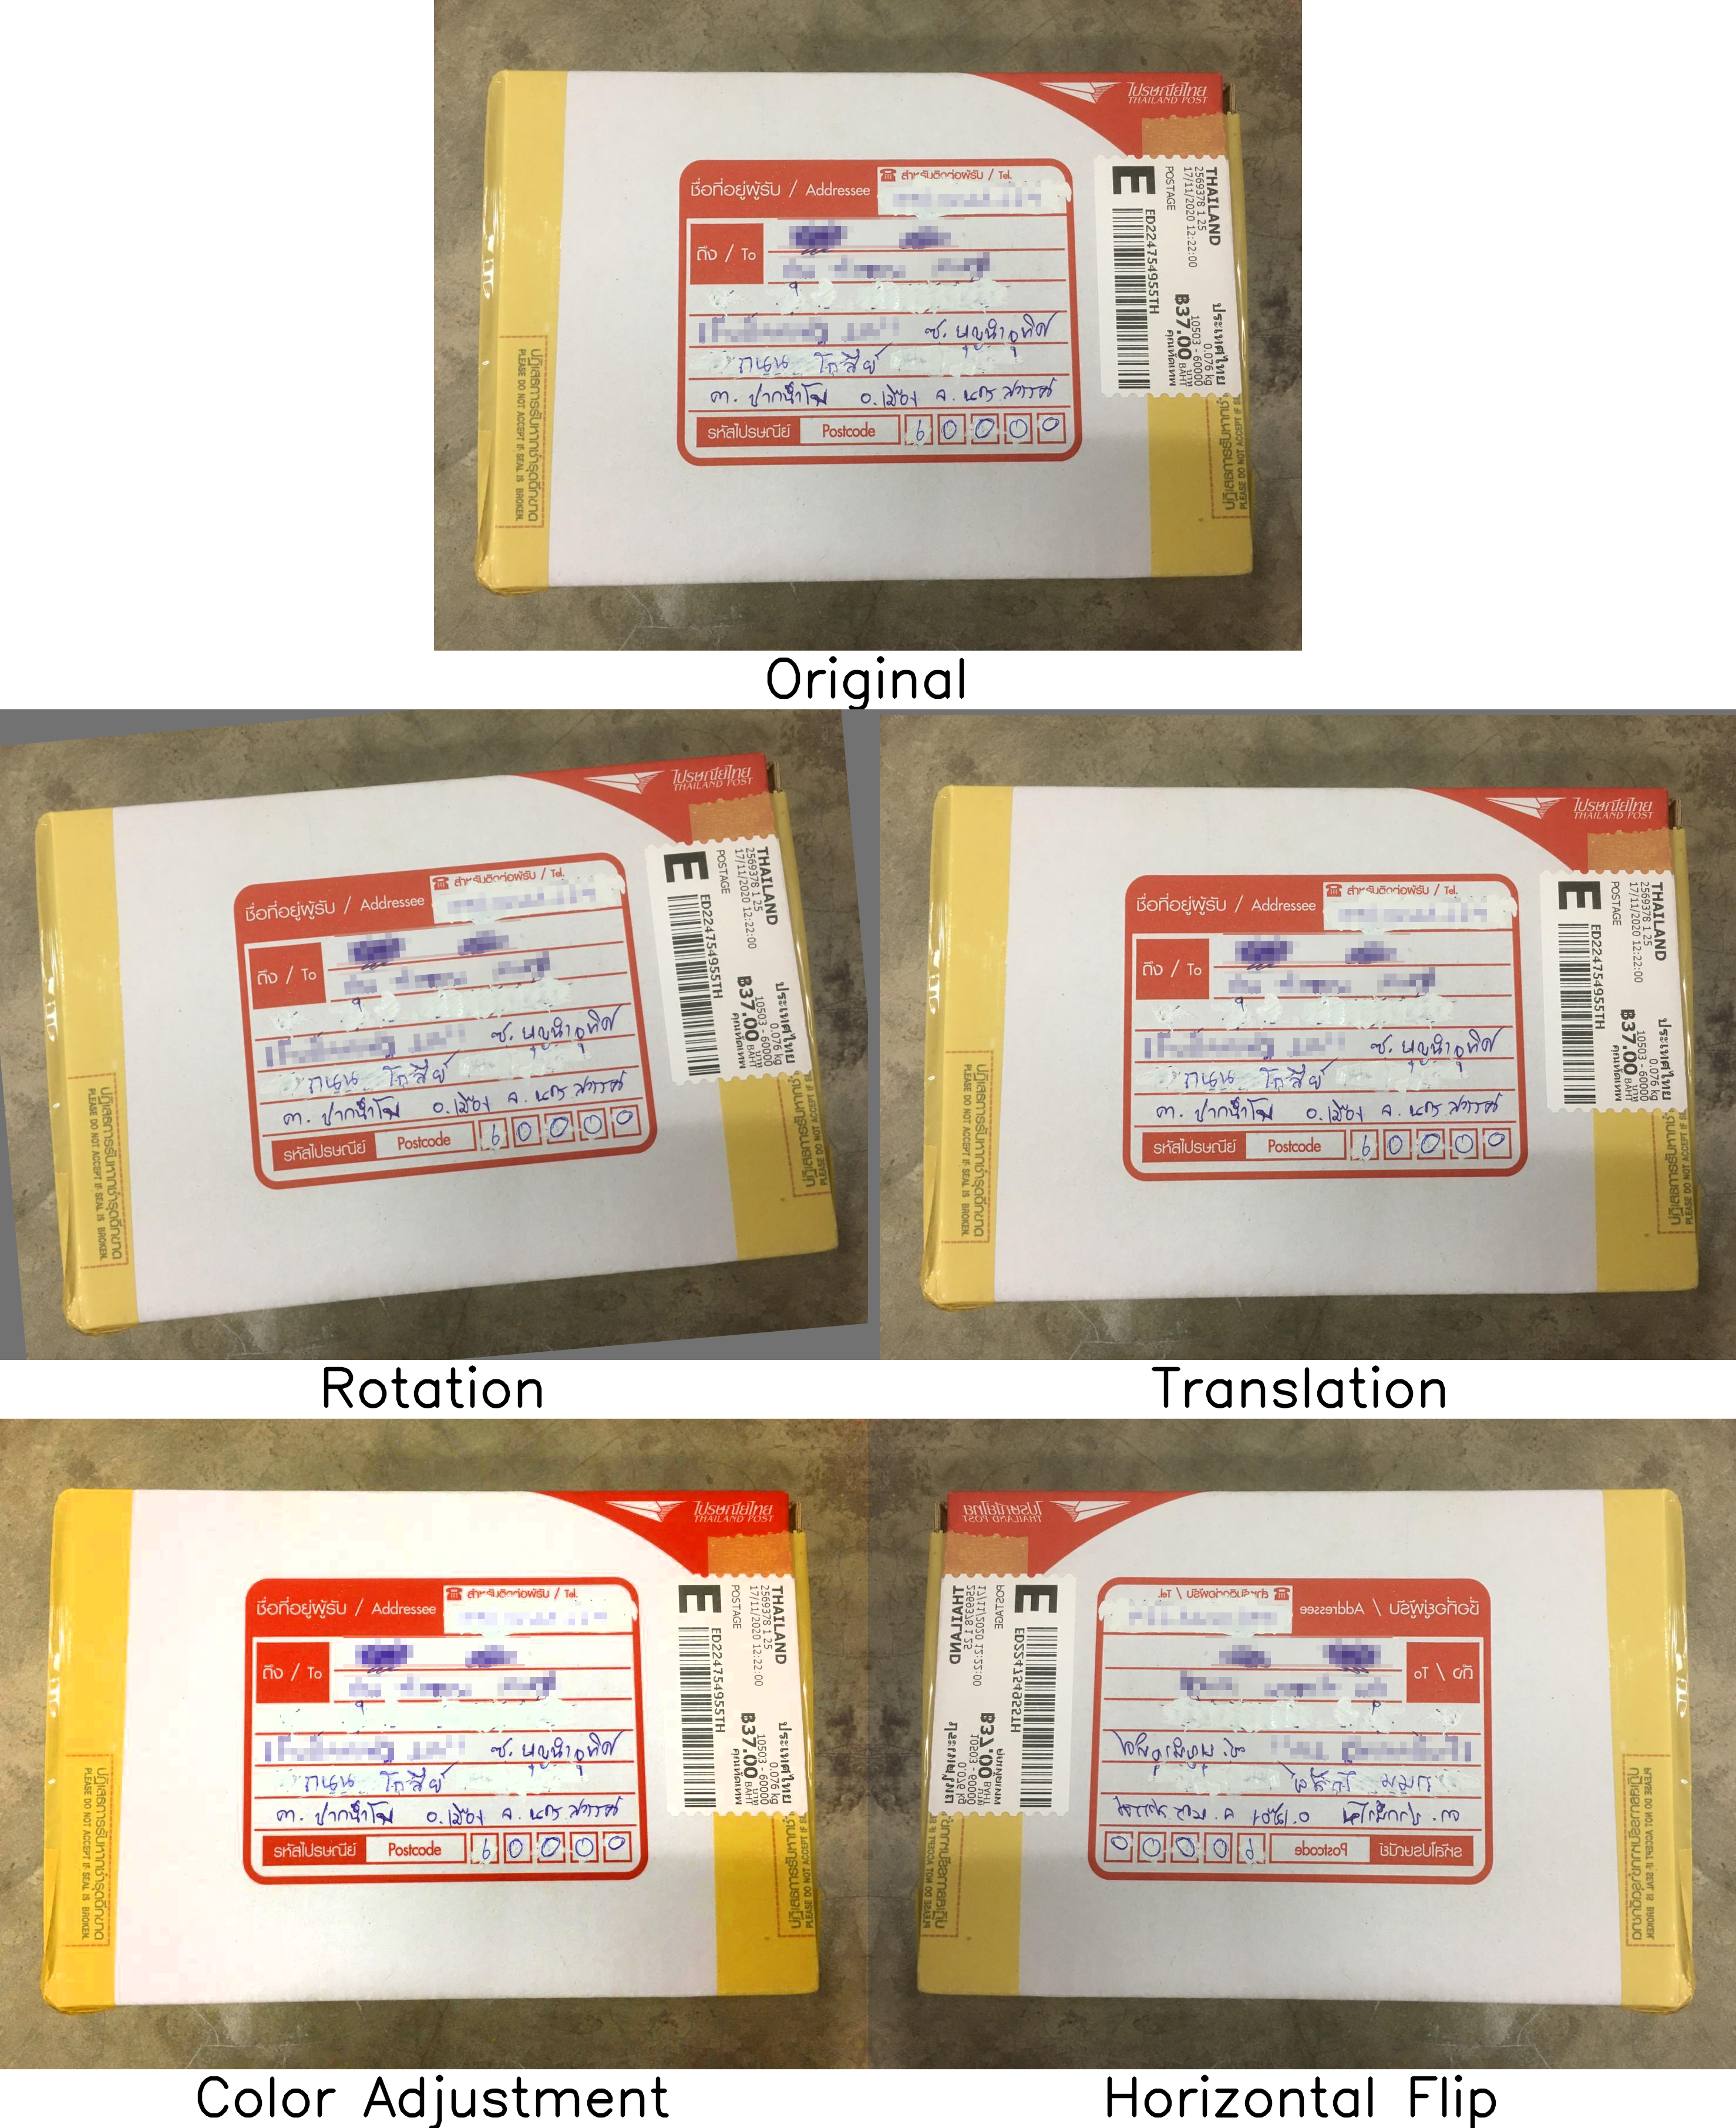
\includegraphics[width=0.7\textwidth]{figures/images/chapter-8/augmentations-example.png}
\caption{
Examples of geometric and photometric augmentations applied during training,
including rotation, translation, color adjustment, and horizontal flipping.
Image source ~\cite{inventbar_kaggle}.
}
\label{fig:data_augmentation_examples}
\end{figure}

The selected augmentations were intended to improve robustness to moderate variation in camera orientation, lighting conditions, and object placement while preserving the visual characteristics of \gls{barcode}s and license plates. The augmentation configuration was implemented directly in the \gls{yolox} experiment file. A simplified excerpt is shown in Listing~\ref{lst:yolox_aug}, while the full configuration is provided in Appendix~\ref{app:yolox_config}.

\methodheading{Model Training}

Model training was performed in \gls{yolox} using pretrained weights from the official \gls{yolox} repository \cite{yolox_github}. This reduced training time and provided a strong baseline for custom detector development. All models used the \gls{yolox-s} architecture. The shared training configuration included a base learning rate of \texttt{0.01 / 64}, 5 warmup epochs, a minimum learning rate ratio of \texttt{0.05}, SGD as optimizer, and 15 no-augmentation epochs.

Training was conducted on a system equipped with an NVIDIA RTX 4080 \gls{gpu} and 32 GB of RAM. As a result, some configuration choices, particularly input resolution and batch size, were selected not only based on validation performance but also to remain within the available memory budget and avoid instability or out-of-memory failures.

The main differences between model versions concerned input resolution, batch size, maximum number of epochs, and augmentation settings. These were adjusted through empirical experimentation in order to balance detection performance, training stability, and hardware constraints. A summary of the training configurations is provided in Appendix~\ref{app:custom_model_evaluation}, while the complete configuration details are included in Appendix~\ref{app:yolox_config}.

\subsubsection{Named Entity Recognition Model Development}

In addition to the image-based object detectors, the project also included the development of a custom named entity recognition (NER) pipeline for detecting sensitive textual information extracted through \acrshort{ocr}. While the \gls{barcode} and license plate models addressed a visual detection problem, the NER component addressed a text understanding problem by identifying sensitive entities directly in recognized text.

The purpose of the NER pipeline was to classify \acrshort{ocr} extracted text into privacy-relevant categories as shown in List~\ref{lst:ner_label_maps}. This made it possible to extend text handling beyond pure \acrshort{ocr} extraction by adding semantic interpretation of the recognized content.

\begin{lstlisting}[caption={BIO label construction for NER training}, label={lst:ner_label_maps}]
ENTITY_LABELS = [
    "PERSON_NAME",
    "PHONE",
    "EMAIL",
    "DATE",
    "ADDRESS",
    "LOCATION",
    "LICENSE_PLATE",
    "POSTAL_CODE",
    "URL",
    "ORGANIZATION",
    "ID_NUMBER",
]
\end{lstlisting}

\methodheading{Dataset Construction}

Since no directly suitable domain-specific dataset was available for all target categories, the NER training data was constructed by combining synthetically generated samples with converted external NER datasets. The synthetic dataset generation pipeline was implemented in \texttt{dataset\_gen.py}, where entity values were sampled from predefined generators and inserted into template-based text examples.

To improve robustness, the generated data included both Norwegian and English text, \acrshort{ocr} like distortions, formatting variation, random casing, typographical noise, and hard negative examples. In addition to short field-based examples, the generator also produced chat-style, form-style, report-style, and document-style samples to better reflect the variability of \acrshort{ocr} derived text in practice.

To strengthen recognition of general linguistic entity categories, two external NER datasets were incorporated into the workflow. The Norwegian NorNE corpus and an English NER dataset were converted into the project’s internal JSONL format and mapped to the \gls{SafeVision} entity schema. These external datasets primarily strengthened recognition of person names, organizations, and locations in natural running text, while the synthetic dataset remained responsible for \acrshort{ocr} specific and privacy specific entity categories such as phone numbers, email addresses, URLs, postal codes, license plates, and identification numbers.

After conversion, the synthetic and external datasets were merged and subsequently divided into training, validation, and test subsets. Detailed dataset composition and split sizes are provided in Appendix~\ref{app:ner_evaluation}.

\methodheading{NER Model Training}

The NER model was trained using XLM-RoBERTa as the encoder backbone through the Hugging Face Transformers framework. The implementation in \texttt{train\_ner.py} used a token classification setup, where each token was assigned a BIO-formatted label corresponding to the underlying entity category.

During preprocessing, character-level entity spans were aligned to tokenizer offsets. Tokens outside annotated spans were assigned the \texttt{O} label, while tokens inside an entity span were assigned \texttt{B-} and \texttt{I-} prefixes depending on whether the token started or continued the entity.
Listning~\ref{ner_align_labels}
\begin{lstlisting}[caption={Span-to-token alignment for BIO labeling}, label={lst:ner_align_labels}]
def align_labels(example, tokenizer, max_length):
    encoding = tokenizer(
        example["text"],
        truncation=True,
        max_length=max_length,
        return_offsets_mapping=True,
    )

    offsets = encoding["offset_mapping"]
    labels = []

    for token_start, token_end in offsets:
        if token_start == token_end:
            labels.append(-100)
        else:
            labels.append(label2id["O"])

    for ent in example["entities"]:
        start, end, label = ent["start"], ent["end"], ent["label"]

        first = True
        for i, (token_start, token_end) in enumerate(offsets):
            if token_start == token_end:
                continue

            if token_start < end and token_end > start:
                prefix = "B" if first else "I"
                labels[i] = label2id[f"{prefix}-{label}"]
                first = False

    encoding["labels"] = labels
    encoding.pop("offset_mapping")
    return encoding
\end{lstlisting}

Training was performed using the Hugging Face \texttt{Trainer} \acrshort{api} with a token classification model initialized from \texttt{FacebookAI/xlm-roberta-base}. The detailed training configuration and evaluation results are provided in Appendix~\ref{app:ner_evaluation}.

\methodheading{\Gls{inference} and Post-Processing}

After training, prediction and evaluation were performed through \texttt{predict\_ner.py}. The token-level predictions produced by the model were merged back into entity spans by grouping adjacent subword predictions and converting them to character offsets in the original text.

\begin{lstlisting}[caption={Merging token predictions into entity spans}, label={lst:ner_merge_spans}]
def merge_subword_spans(labels, offsets, probs, text, threshold=0.0):
    entities = []
    current = None

    for label, (start, end), score in zip(labels, offsets, probs):
        if start == end:
            continue

        if label == "O" or score < threshold:
            if current is not None:
                entities.append(current)
                current = None
            continue

        if "-" in label:
            prefix, entity_type = label.split("-", 1)
        else:
            prefix, entity_type = "B", label

        if prefix == "B":
            if current is not None:
                entities.append(current)
            current = {
                "start": start,
                "end": end,
                "label": entity_type,
                "scores": [score],
            }

        elif prefix == "I":
            if current is not None and current["label"] == entity_type:
                current["end"] = max(current["end"], end)
                current["scores"].append(score)
\end{lstlisting}

\acrshort{ocr} derived text often contains noise, inconsistent punctuation, and formatting wrappers, the raw spans were further post-processed before final evaluation. This included trimming punctuation, removing common textual prefixes such as field labels, stripping suffix wrappers, and applying lightweight heuristics for labels such as listed in Listning~\ref{lst:ner_align_labels}.

In the final system, the NER model complemented the \acrshort{ocr} subsystem by adding a text-level interpretation layer for privacy-sensitive content, but it was not used as a standalone text classification component. Instead, \acrshort{ocr} extracted text was processed through a hybrid text-analysis pipeline, implemented in
\texttt{pii\_detector.py} (Appendix~\ref{app:pii_detector}), where NER predictions were combined with contextual rules and post-processing heuristics. This was done because standalone NER predictions were less reliable on practical document inputs than the constructed evaluation results initially
suggested.

\section{AI/\acrshort{ml} Integration}
\label{ai_ml_integration}
This section describes how \acrshort{ml} models are integrated into the system to support detection of sensitive information. It outlines the structure of the detection engine and the strategy used to load and execute the individual models.

\methodheading{Detection Engine Architecture}

The detection engine combines several task-specific \acrshort{ml} models within a common framework. Each model is responsible for detecting a distinct category of sensitive information. An overview of the detection models and their capabilities is shown in Table~\ref{tab:detection_models}.

\begin{table}[H]
\centering
\small
\begin{tabularx}{\textwidth}{|p{2.7cm}|p{4.4cm}|X|}
\hline
\textbf{Engine} & \textbf{Technology} & \textbf{Capabilities} \\ \hline

\textbf{RetinaFace} & 
CNN-based face detector & 
Face detection with high accuracy and robustness to scale and pose. \\ \hline

\textbf{PaddleOCR} & 
\acrshort{ocr} framework (detection + recognition) & 
Text detection and recognition in natural scenes. \\ \hline

\textbf{XLM-RoBERTa NER} & 
Transformer-based token classification model & 
Identification of sensitive entities in \acrshort{ocr} extracted text. \\ \hline

\textbf{YOLOX} & 
Real-time \gls{object detection} (YOLO-based) & 
\gls{barcode}, license plate, and general \gls{object detection}. \\ \hline

\end{tabularx}
\caption{Overview of AI/\acrshort{ml} models used in the system.}
\label{tab:detection_models}
\end{table}

Although the models serve different tasks, they are integrated into a shared processing workflow. The image-based models operate on comparable visual inputs, while the NER model processes text extracted through \acrshort{ocr}. Their outputs are subsequently normalized into a shared representation that supports downstream filtering, review, and redaction. This simplifies integration and makes it easier to extend the system with additional detectors or text-analysis components. The detection engine is integrated with the processing pipeline described in Section~\ref{Preprocessing_subsection} and Section~\ref{subsec:post_processing}, where preprocessing, \gls{inference}, and post-processing are handled in sequence.

\methodheading{Model Integration and Execution}

The models follow a common integration pattern in order to keep the system simple and maintainable. Each detector is implemented in its own module, while model instances are loaded as shared resources to avoid repeated initialization. Therefore lazy loading is used to defer model initialization until a detector is first requested. This is implemented through helper functions such as \texttt{get\_face\_detector()} in \texttt{backend/controllers/detect\_controller.py}, which create the model instance on first use and return the same instance for subsequent requests.

\begin{lstlisting}[caption={Lazy loading of detection model}, label={lst:lazy_loading}]
def get_face_detector():
    global detector
    if detector is None:
        detector = load_model()
    return detector
\end{lstlisting}

Listing~\ref{lst:lazy_loading} shows how model initialization is deferred until first use and how the same instance is reused across requests. This structure improves code organization and makes it possible to add new detectors without requiring major changes elsewhere in the backend.

\section{Image Processing and Redaction Pipeline}
\label{image_processing_and_redaction_pipeline}

This section describes the processing steps applied to image data before and after model \gls{inference}. While the detection pipeline (Section~8.3.2) focuses on identifying sensitive entities, this component is responsible for preparing input data, transforming detection results, and applying \gls{anonymization} techniques. The implementation is primarily located in the pipeline modules under \texttt{pipeline/common}.


\methodheading{Preprocessing}
\label{Preprocessing_subsection}

The preprocessing stage prepares input images before they are passed to the detection models. This includes optional scaling and enhancement operations, which can improve detection accuracy, particularly for small or low-resolution objects. Scaling is used to balance performance and accuracy, where downscaling can reduce computation time and upscaling can improve detection of small features. Preprocessing operations are shared across multiple detection modules and ensure that all models operate on a consistent input representation.

In addition to manual scaling, the system supports adaptive scaling based on the requirements of individual detection models. When enabled, the image is automatically resized such that its resolution better matches the expected input size of the selected model. This is implemented through a model-aware preprocessing step, where the scaling factor is computed dynamically based on the model’s preferred input resolution. Listing~\ref{lst:adaptive_preprocessing} shows how adaptive scaling is integrated with the standard preprocessing pipeline. The system adjusts image resolution based on the selected model, while still reusing the same preprocessing logic.

\begin{lstlisting}[caption={Model-aware preprocessing with adaptive scaling}, label={lst:adaptive_preprocessing}]
def preprocess_for_model(
    img_bgr,
    h0,
    w0,
    model_name,
    adaptive_scaling,
    base_scale,
    use_preprocess,
):
    if adaptive_scaling:
        model_input = MODEL_INPUT_SIZES.get(model_name, 640)
        scale = model_input / max(h0, w0)
        scale = max(0.5, min(scale, 2.0))
    else:
        scale = base_scale

    img_proc, total_scale, used_preprocess = preprocess_image(
        img_bgr,
        scale=scale,
        use_preprocess=use_preprocess,
    )

    return img_proc, total_scale, used_preprocess
\end{lstlisting}

Adaptive scaling can improve detection accuracy, particularly for models that are sensitive to input resolution. However, it introduces additional computational cost due to image resizing. For this reason, it is implemented as an optional feature that can be enabled or disabled by the user. By default, adaptive scaling is enabled to prioritize detection accuracy, while still allowing performance-oriented configurations.

\methodheading{Bounding Box Processing}
\label{subsec:post_processing}

After detection, \gls{bounding box} processing is performed as a post-processing step to normalize outputs from different models into a unified format. This involves validating coordinates, clamping values to image boundaries, and ensuring that all \gls{bounding box}es are well-formed. The process also includes geometric transformations such as scaling and coordinate adjustment, which are necessary when preprocessing steps modify the image resolution. Additionally, \gls{bounding box}es may be expanded to include contextual regions, which is useful for \gls{segmentation} based \gls{masking}. These operations are implemented through utility functions that ensure robustness against invalid or out-of-bounds detections.

\methodheading{\Gls{segmentation} and Mask Generation}

To enable more precise redaction, the system supports \gls{segmentation} based \gls{masking} using \gls{mobilesam}. When \gls{segmentation} is requested, the system extracts a region of interest around the detected \gls{bounding box} and uses it as input to the \gls{segmentation} model. The resulting binary mask represents the object more accurately than a rectangular \gls{bounding box}, allowing for higher quality \gls{anonymization}.

The implementation includes several safeguards to ensure stability. If the \gls{segmentation} model is unavailable or fails to produce a valid mask, the system automatically falls back to \gls{bounding box} \gls{masking}. The generated masks are further refined using morphological operations, such as opening, closing, and smoothing, to remove noise and improve visual quality. Listing~\ref{lst:mask_refinement} illustrates how mask refinement is implemented in \texttt{anonymize.py}.

\begin{lstlisting}[caption={Mask refinement using morphological operations}, label={lst:mask_refinement}]
kernel = np.ones((5, 5), np.uint8)
mask = cv2.morphologyEx(mask, cv2.MORPH_OPEN, kernel)
mask = cv2.morphologyEx(mask, cv2.MORPH_CLOSE, kernel)
mask = cv2.GaussianBlur(mask, (9, 9), 0)
\end{lstlisting}

\methodheading{Redaction Methods}

This stage of the pipeline applies \gls{anonymization} to the detected regions. The functionality is implemented in \texttt{anonymize.py}, which provides a common interface for different redaction methods. The system supports blurring, pixelation, black-box \gls{masking}, and \gls{inpainting}. These methods are applied to selected regions using masks to blend the result with the original image.

\begin{lstlisting}[caption={Applying redaction to detected regions}, label={lst:anonymize_call}]
def anonymize(img, boxes, method="blur", mask_mode="segmentation"):
    out = img.copy()

    for box in boxes:
        roi_data = _get_roi_and_mask(img, out, box, pad_ratio=0.05, mask_mode=mask_mode)
        if roi_data is None:
            continue

        box_coords, roi, mask = roi_data

        _apply_method(method, out, roi, mask, pixel_size=40, inpaint_radius=7, box_coords=box_coords)

    return out
\end{lstlisting}

Listing~\ref{lst:anonymize_call} shows how redaction methods are applied to detected regions. For each \gls{bounding box}, a region of interest and corresponding mask are extracted, after which the selected \gls{anonymization} method is applied. This design enables flexible and consistent processing across different \gls{masking} strategies.

\begin{table}[H]
\centering
\begin{tabular}{lcc}
\hline
\textbf{Method} & \textbf{Visual Effect} & \textbf{Use Case} \\
\hline
Blur & Smooth distortion & Faces / privacy-friendly \gls{masking} \\
Pixelate & Block-based \gls{masking} & Strong \gls{anonymization} \\
Blackbox & Full occlusion & Maximum privacy \\
Inpaint & Background reconstruction & Aesthetic output \\
\hline
\end{tabular}
\caption{Comparison of redaction methods.}
\label{tab:redaction_methods}
\end{table}

Table~\ref{tab:redaction_methods} summarizes the available methods and their typical use cases. Blurring and pixelation reduce detail while keeping the general structure of the image. Black-box \gls{masking}, on the other hand, completely hides the selected region. \Gls{inpainting} works differently by filling the region using surrounding pixel information.

The system supports both \gls{bounding box} and \gls{segmentation} masks, and allows different methods to be applied to different regions. This makes it possible to balance privacy and visual quality depending on the  case.



\section{Video Implementation}
\label{sec:video_imp}

This section describes how video processing was implemented in \gls{SafeVision}. It explains how videos are decoded, how \gls{bounding box}es are propagated between detection frames and how the manual video tracking is handled.

\methodheading{Video Detection Integration}

Video detection is handled through the \texttt{POST /api/video/detect} endpoint and is implemented through \texttt{video\_detect\_controller.py} together with additional functionality. Uploaded videos are first stored in a temporary working directory before OpenCV is used to open the file and read video metadata. Using this method, \gls{SafeVision} can decode the video frame by frame by reading the frame rate and dimensions. Detection is not performed on every frame. The video iteration is handled by \texttt{iter\_video\_live} and the wrapper \texttt{extract\_video\_live}, while \texttt{detect\_live\_on\_frame} applies detection to the selected frames.

The frame-level detection function uses the same detection infrastructure as the image pipeline, including all preprocessing and models. This means that video does not use its own separate detection system, but instead applies the image-based detection already implemented in \gls{SafeVision} repeatedly to decoded frames. The result is returned as a manifest of all frames with a frame index, frame timestamp and a list of detections. This manifest is later used to create \gls{bounding box}es for review and redaction in a similar way as for images.

\methodheading{Prediction and Bounding Box Propagation}

As previously stated, the video pipeline does not run full image detection on every frame by default. Since \gls{SafeVision} reuses the same detectors for images and video, full detection on every frame can be computationally expensive. Therefore, an option is implemented for the user to decide the program's detection frequency. This is handled through the \texttt{detect\_every} parameter, which specifies detection on every Nth frame. A lower value runs detection more frequently, allowing the user to balance processing time against video detection accuracy.

Between detection frames, \gls{bounding box}es are propagated using \texttt{kalman\_multi\_tracker.py}. This implementation follows the video tracking approach introduced in Section~\ref{sec:video_tracking_foundation}, where Kalman-based prediction, entity-specific matching, interpolation, and backfilling are used to maintain temporally consistent \gls{bounding box}es between sparse detection frames. For each frame, the \gls{kalman filter} predicts the next position of active \gls{bounding box}es based on their previous location and movement. This allows detected regions to remain present in frames where the detector is not executed, reducing the risk that sensitive content disappears between detection intervals.

When a new detection frame is reached, the backend runs \texttt{detect\_live\_on\_frame(...)} and matches the new detections with existing predicted boxes. This matching is performed separately for each entity type. If a new detection matches an existing prediction, the \gls{kalman filter} corrects the predicted position using the detected box. If a detection does not match any existing prediction, a new prediction state is created, indicating that a new sensitive object may have appeared in the video. Prediction states that remain unmatched for too long are eventually stopped, since this indicates that the object is no longer visible. This flow is illustrated in Figure~\ref{fig:video_tracking_flow}.

\begin{figure}[H]
\centering
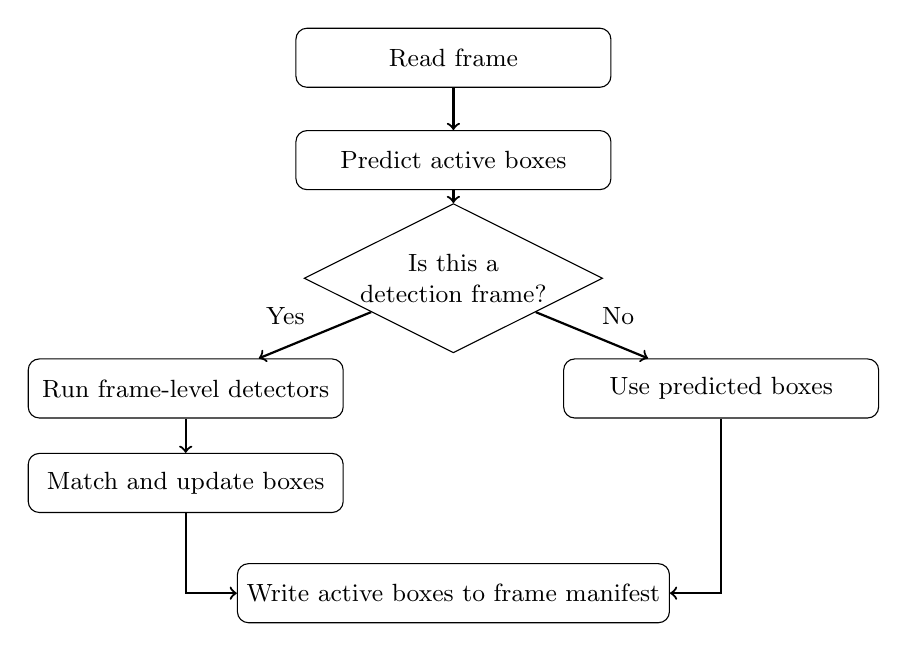
\begin{tikzpicture}[
    every node/.style={font=\small},
    box/.style={
        rectangle,
        rounded corners,
        draw=black,
        minimum width=4.0cm,
        minimum height=0.75cm,
        align=center
    },
    widebox/.style={
        rectangle,
        rounded corners,
        draw=black,
        minimum width=5.4cm,
        minimum height=0.75cm,
        align=center
    },
    decision/.style={
        diamond,
        draw=black,
        aspect=2,
        align=center,
        inner sep=1pt,
        minimum width=2.8cm,
        minimum height=1.1cm
    },
    arrow/.style={->, thick}
]

% Nodes with fixed coordinates
\node[box]      (read)     at (0, 0)      {Read frame};
\node[box]      (predict)  at (0, -1.3)   {Predict active boxes};
\node[decision] (detectq)  at (0, -2.8)   {Is this a\\ detection frame?};

\node[box]      (detect)   at (-3.4, -4.2) {Run frame-level detectors};
\node[box]      (match)    at (-3.4, -5.4) {Match and update boxes};

\node[box]      (usepred)  at (3.4, -4.2)  {Use predicted boxes};

\node[widebox]  (manifest) at (0, -6.8)    {Write active boxes to frame manifest};

% Arrows
\draw[arrow] (read) -- (predict);
\draw[arrow] (predict) -- (detectq);

\draw[arrow] (detectq) -- node[above left] {Yes} (detect);
\draw[arrow] (detect) -- (match);

\draw[arrow] (detectq) -- node[above right] {No} (usepred);

\draw[arrow] (match.south) |- (manifest.west);
\draw[arrow] (usepred.south) |- (manifest.east);

\end{tikzpicture}
\caption{Simplified flow of video detection and prediction. For each frame, the \gls{kalman filter} first predicts active regions. If the frame is selected for detection, frame-level detectors are executed and matched with existing predictions. Otherwise, the predicted boxes are used directly before the frame data is written to the manifest.}
\label{fig:video_tracking_flow}
\end{figure}

\methodheading{Manual Tracking}

Manual tracking is handled separately from the automatic Kalman-based prediction. For images, manual boxes are drawn and can be redacted directly, but in video a manually drawn box would either only affect the single frame where it was drawn or remain as a stationary box over a span of frames. Therefore, to make manual redaction usable for video, \gls{SafeVision} includes a dedicated manual tracking endpoint, \texttt{POST /api/video/track-manual}. This endpoint receives the video and the existing manifest, regardless of whether it already contains Kalman-predicted boxes, and adds the manually tracked region across the relevant frames. The implementation is mainly located in \texttt{video\_track\_manual\_controller.py} and \texttt{manual\_single\_tracker.py}.

Manual tracking is handled by \texttt{track\_manual\_box\_in\_manifest}, which initializes tracking from the selected frame and the region selected by the user. Unlike the automatic Kalman-based prediction, this manual tracking path uses an OpenCV object tracker to follow the user-defined region through the video. The implementation primarily uses TrackerViT, while Channel and Spatial Reliability Tracking (CSRT) is included as a fallback tracker. This connects the implementation to the tracking methods introduced in Section~\ref{sec:video_tracking_foundation}. The selected region is tracked both forward and backward from the chosen frame, and manual tracks are assigned negative track IDs so that they do not collide with automatically generated track IDs.

\begin{figure}[H]
\centering

\begin{subfigure}{0.48\textwidth}
    \centering
    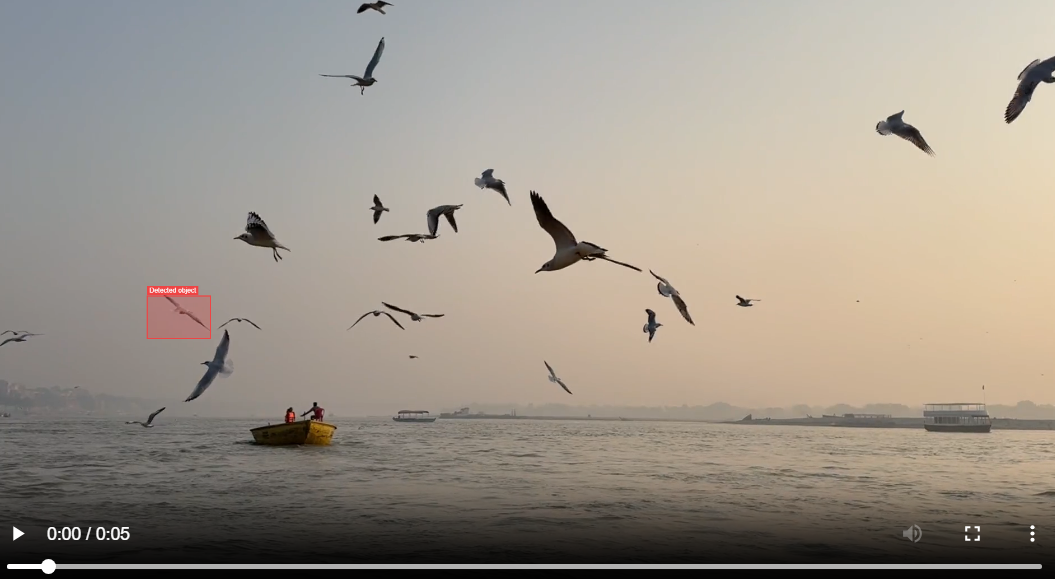
\includegraphics[width=\textwidth]{figures/images/chapter-8/bird1.png}
    \caption{Manual \gls{bounding box} initialized on a bird in the selected frame.}
\end{subfigure}
\hfill
\begin{subfigure}{0.48\textwidth}
    \centering
    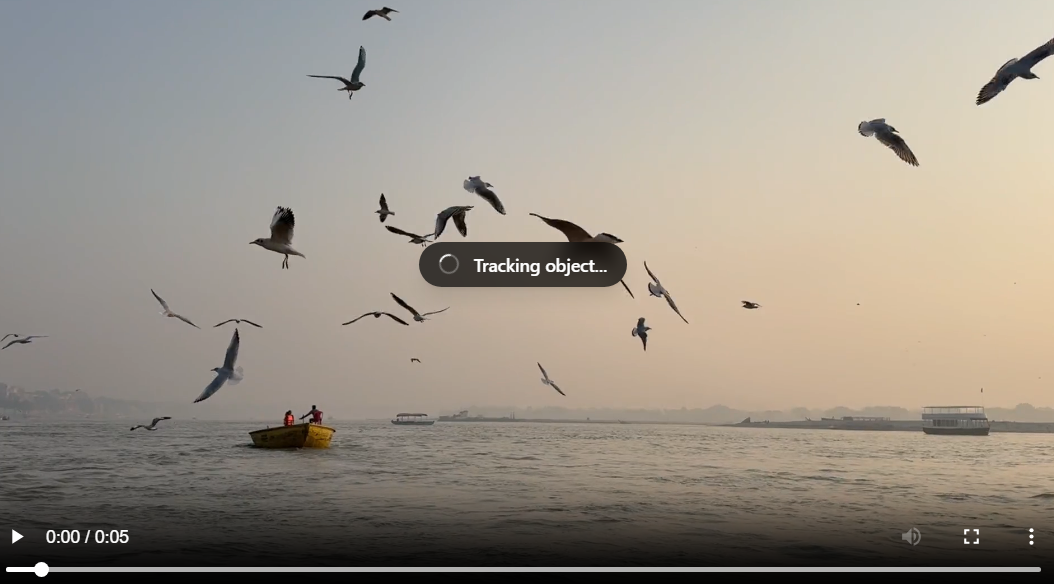
\includegraphics[width=\textwidth]{figures/images/chapter-8/bird2.png}
    \caption{Tracker propagated to other frames in the video.}
\end{subfigure}

\vspace{0.4cm}

\begin{subfigure}{0.48\textwidth}
    \centering
    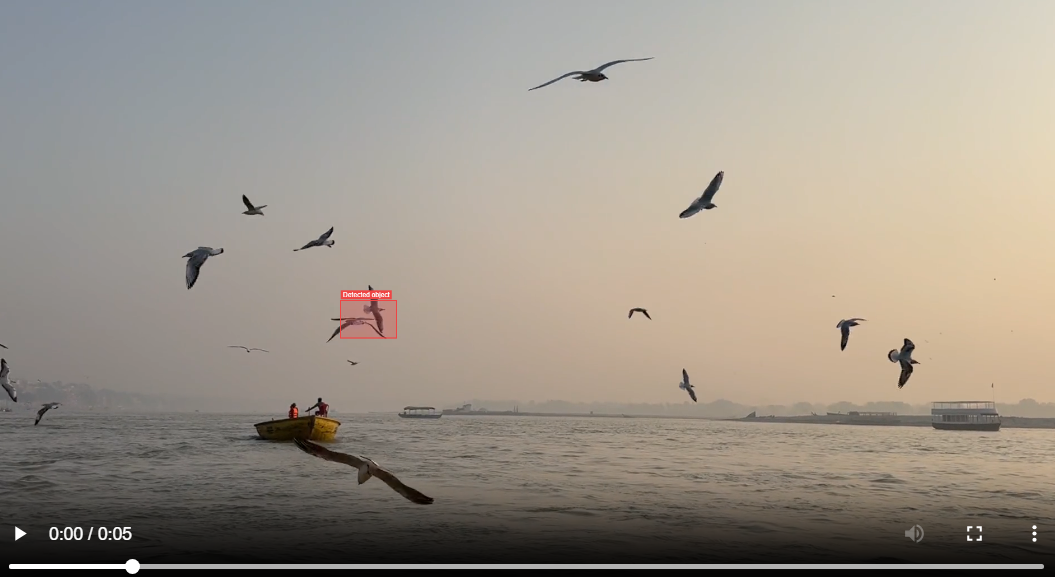
\includegraphics[width=\textwidth]{figures/images/chapter-8/bird3.png}
    \caption{Bird flies through an area with low tracking certainty.}
\end{subfigure}
\hfill
\begin{subfigure}{0.48\textwidth}
    \centering
    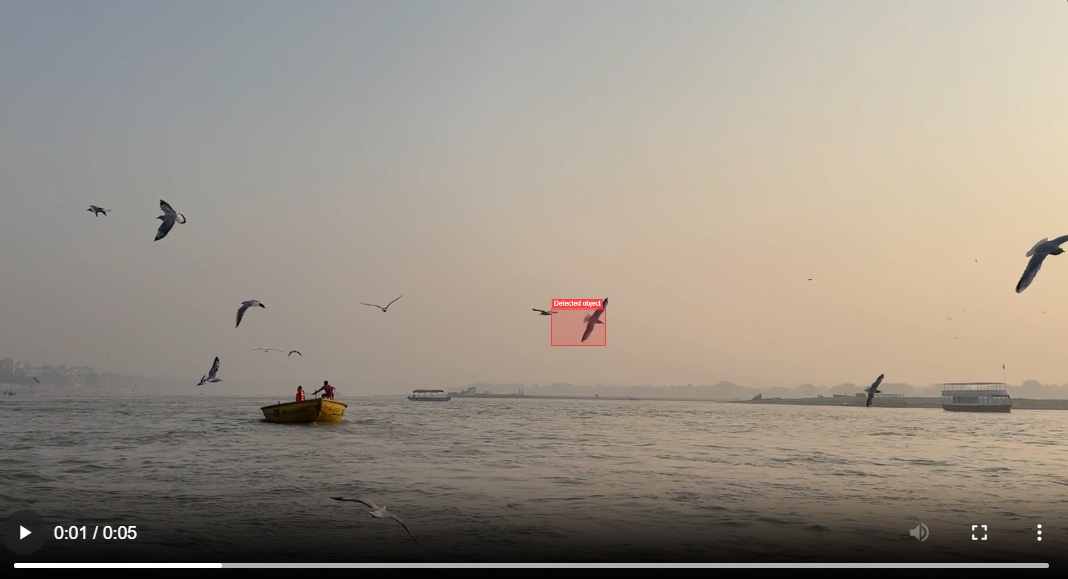
\includegraphics[width=\textwidth]{figures/images/chapter-8/bird4.png}
    \caption{Successfully tracked the bird through the flock.}
\end{subfigure}

\caption{Example of manual video tracking in \gls{SafeVision}. A manually drawn \gls{bounding box} is initialized on one frame and propagated through later frames. Source video by~\cite{pexels_shubh_agrawal_video}.}
\label{fig:manual_video_tracking_sequence}
\end{figure}


The manual tracking implementation includes safeguards to reduce unstable tracking results from either TrackerViT or the \acrshort{csrt} fallback. Functions such as \texttt{\_is\_suspicious} and \texttt{\_replay\_safety\_candidate} are used when the tracker output appears unreliable. These checks handle sudden changes in size or aspect ratio, large jumps in position, weak overlap with the last trusted box, or abnormal growth of the tracked object near the frame border. When tracking gives low certainty, the system can temporarily keep the last trusted box, add only the new predicted area of the tracked object as a union, and later replay tracking from a safer region. This makes the manual tracking more reliable than applying raw tracker output directly.

\methodheading{Video Redaction Pipeline}

Video redaction is handled through the \texttt{POST /api/video/redact} endpoint and is controlled through \texttt{video\_redact\_controller.py}. When redaction is run, it receives the original video together with the frame-wise manifest as a blueprint for what to redact. The backend reads the video frame by frame and matches each frame with the corresponding detections listed in the manifest using the function \texttt{redact\_frame\_with\_live}.

The function \texttt{redact\_frame\_with\_live} reuses the existing redaction logic through \texttt{anonymize}, allowing the video pipeline to use the same methods and settings as for images. This means that a video can use blackbox, blur, pixelation, \gls{inpainting} and \gls{segmentation} for the relevant box categories. After processing all frames, OpenCV is used to write a temporary video output, and \texttt{remux\_to\_h264\_aac} in \texttt{ffmpeg\_utils.py} finalizes the complete redacted video before temporary files are cleaned up.


\section{Deployment}

This section describes how the deployment architecture and infrastructure presented in Chapter~\ref{chap:technologies_and_methodologies} (Figure~\ref{fig:deployment_architecture}) are implemented in practice. The deployment setup ensures reproducibility, scalability, and efficient handling of both frontend and backend components.

\methodheading{Continuous Integration and Deployment}

The system uses GitHub Actions to implement both continuous integration (CI) and continuous deployment (CD) as part of the development workflow.

\begin{figure}[H]
    \centering
    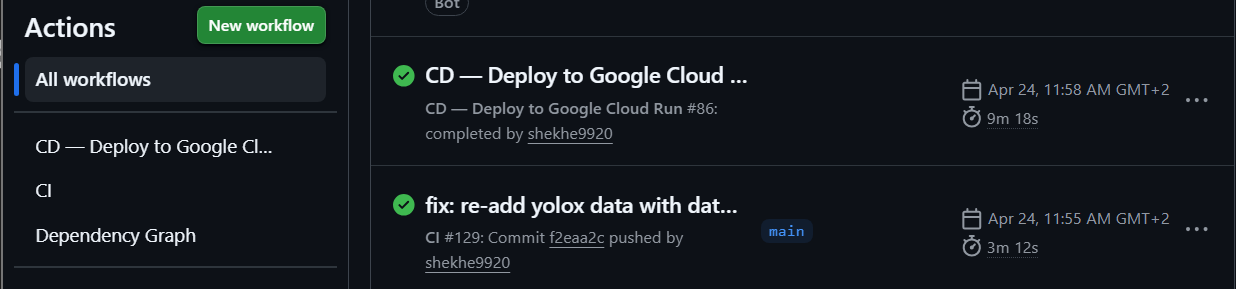
\includegraphics[width=0.85\textwidth]{figures/images/chapter-8/github-actions-workflow.png}
    \caption{Example of successful CI and CD workflow executions in GitHub Actions. The workflows were used to validate frontend and backend changes before deploying updated application artifacts.}
    \label{fig:github_actions_workflow}
\end{figure}

\paragraph{Continuous Integration (CI)}

The CI pipeline is triggered on every push or pull request to the main branch and is responsible for validating both frontend and backend components. For the frontend, the pipeline installs dependencies using npm, performs linting and type checking, runs tests, and builds the application to ensure that the code compiles correctly. For the backend, the pipeline installs Python dependencies, performs static analysis using Ruff, and executes unit tests using pytest. To enable testing without requiring \acrshort{ml} model weights, a configuration flag (\texttt{ALLOW\_FAKE\_DETECTORS}) is used to bypass model loading during CI execution. An excerpt of the CI pipeline is shown in Listing~\ref{lst:ci_pipeline}.

\begin{lstlisting}[caption={Excerpt from CI pipeline using GitHub Actions}, label={lst:ci_pipeline}]
jobs:
  frontend:
    runs-on: ubuntu-latest
    steps:
      - uses: actions/checkout@v4
      - uses: actions/setup-node@v4
      - run: npm ci
      - run: npm run lint --if-present
      - run: npm test --if-present
      - run: npm run build

  backend:
    runs-on: ubuntu-latest
    env:
      ALLOW_FAKE_DETECTORS: "true"
    steps:
      - uses: actions/checkout@v4
      - uses: actions/setup-python@v5
      - run: pip install -r requirements.txt
      - run: ruff check .
      - run: pytest -q
\end{lstlisting}

\paragraph{Continuous Deployment (CD)}

The CD pipeline is triggered after successful CI execution and is responsible for building and deploying the application. The backend is built into a Docker container using Google Cloud Build, pushed to Artifact Registry, and deployed to Google Cloud Run as a managed service. The frontend is built and deployed as a static application to Google Cloud Storage. An excerpt of the deployment pipeline is shown in Listing~\ref{lst:cd_pipeline}.

\begin{lstlisting}[caption={Excerpt from CD pipeline for deployment to Google Cloud}, label={lst:cd_pipeline}]
- name: Build container image
  run: |
    gcloud builds submit \
      --tag europe-north1-docker.pkg.dev/${{ secrets.GCP_PROJECT_ID }}/cv-backend/cv-api

- name: Deploy to Cloud Run
  run: |
    gcloud run deploy cv-api \
      --image europe-north1-docker.pkg.dev/${{ secrets.GCP_PROJECT_ID }}/cv-backend/cv-api \
      --region europe-north1 \
      --platform managed
\end{lstlisting}

\methodheading{Backend Deployment}

The backend container as shown in Listing~\ref{lst:dockerfile}, is built from a lightweight Python base image and includes system-level dependencies required for OpenCV and video processing. \acrshort{ml} libraries are installed using CPU-based configurations to ensure compatibility with the Cloud Run environment. This setup ensures a reproducible and portable runtime environment, where all dependencies are packaged within the container and can be deployed consistently across environments.

\begin{lstlisting}[caption={Simplified Dockerfile for backend deployment}, label={lst:dockerfile}]
FROM python:3.12-slim

WORKDIR /app

# System dependencies for image processing
RUN apt-get update && apt-get install -y --no-install-recommends \
    ffmpeg libgl1 libglib2.0-0 \
    && rm -rf /var/lib/apt/lists/*

# Install Python dependencies (CPU-only ML setup)
COPY requirements-prod.txt .
RUN pip install --no-cache-dir \
    --index-url https://download.pytorch.org/whl/cpu \
    torch torchvision torchaudio && \
    pip install -r requirements-prod.txt

# Copy application
COPY backend/ ./backend

# Run API
CMD ["uvicorn", "backend.main:app", "--host", "0.0.0.0", "--port", "8080"]
\end{lstlisting}

The backend service is exposed through a FastAPI application running on port 8080, which is the default port expected by Cloud Run. The container is deployed as a managed service on Google Cloud Run, allowing automatic scaling based on incoming request load. In practice, the deployment process is integrated into the CD pipeline (Listing~\ref{lst:cd_pipeline}), where a new container image is built and deployed upon successful CI execution. This ensures that backend updates are consistently packaged and released through an automated workflow.

\methodheading{Frontend Deployment}

During CI, the frontend was validated and built using the standard production build process. This generated a compiled \texttt{dist/} directory containing the static HTML, CSS, and JavaScript assets used for deployment. These files were treated as the release artifact of the frontend and were used as the basis for deployment. During CD, the contents of this directory were uploaded to the hosting environment and served as a static web application. As a result, the frontend did not require a separate application server, and updates could be released by replacing the previously hosted assets with a new production build.

The frontend was configured to communicate with the backend \acrshort{api} through a deployment-specific base URL. This configuration was injected at build time, allowing the same codebase to be used across development and deployed environments while changing only the target \acrshort{api} endpoint. Since the frontend was deployed as static assets, it could be released independently of the backend container. This simplified frontend updates and made it possible to deploy interface changes without rebuilding the backend service.

\methodheading{Model and Environment Configuration}

\acrshort{ml} models are included as part of the backend deployment and selectively uploaded using a customized \texttt{.gcloudignore} configuration. This ensures that only required model weights are included, while unnecessary files such as datasets and training artifacts are excluded. Models are loaded lazily at runtime and reused across requests to reduce initialization overhead and improve performance. In cases where model resources are unavailable, fallback mechanisms are used to maintain system functionality.

The system behavior is further controlled through environment variables, enabling flexible configuration across development, testing, and production environments. For example, the \texttt{ALLOW\_FAKE\_DETECTORS} flag is used in CI environments to disable model loading, allowing tests to run without requiring large model files.


\chapter{Quality Assurance}
\label{chap:testing_system_evaluation}

This chapter presents the quality assurance activities used to evaluate \gls{SafeVision}. It describes the overall testing strategy, including frontend testing, backend testing, user testing, performance testing, and security evaluation. The purpose of the chapter is to assess both the technical correctness of the system and its practical suitability for detecting, reviewing, and anonymizing sensitive information in visual media.


\section{Testing Strategy}

A layered testing strategy was used to evaluate \gls{SafeVision}. At the lowest level, unit tests were written for utility functions, state management, and isolated processing logic. On top of this, integration oriented tests were used for workflows where several hooks, components, or services had to work together. Finally, user oriented evaluation was performed through manual exploratory testing and structured user tests on realistic image and video scenarios in order to assess both practical usability and hybrid workflow behavior.

This combination was chosen because no single testing method was sufficient on its own. Unit tests gave fast feedback and were useful for regression prevention, while integration tests validated interactions across components and services. Manual and user based testing were necessary for evaluating workflows involving file handling, media rendering, and user-controlled redaction, where visual feedback and interaction design played a central role.

In addition to verifying correctness and usability, the user-oriented evaluation was also used to better understand practical user needs. Feedback from real users and users with experience in image and video editing provided insight into different aspects for the system.

\section{Frontend Testing}

Frontend testing was conducted using Vitest in combination with React Testing Library within a JSDOM-based environment. This setup was well suited to the React and Vite architecture of \gls{SafeVision}, allowing both isolated logic and component-level interactions to be tested in a lightweight and reproducible manner.

The frontend test suite covered functionality central to the \gls{SafeVision} workflow, including file handling, consent management, detection and highlight state, workspace interaction, and media controls. Tests also covered utility functions related to image editing, canvas export, video playback, and manifest handling. Since the system supports both images and video, the test suite included checks for frame based operations and synchronization of state across video interactions. This helped verify that core user workflows remained stable across both image and temporal media processing.

\begin{table}[H]
\centering
\small
\begin{tabular}{lcccc}
\hline
\textbf{Module} & \textbf{Statements} & \textbf{Branches} & \textbf{Functions} & \textbf{Lines} \\
\hline
Overall Coverage      & 47.58\% & 38.22\% & 51.37\% & 49.82\% \\
Application Core      & 65.45\% & 45.83\% & 17.64\% & 70.58\% \\
Detection Features    & 50.70\% & 30.43\% & 52.00\% & 47.16\% \\
File Management       & 60.72\% & 29.05\% & 63.23\% & 62.96\% \\
User Preferences      & 50.98\% & 41.66\% & 36.84\% & 56.81\% \\
Workspace Components  & 66.66\% & 66.66\% & 63.63\% & 64.28\% \\
Workspace Hooks       & 32.02\% & 13.00\% & 52.17\% & 35.06\% \\
Image Processing      & 21.48\% & 4.87\%  & 18.75\% & 22.03\% \\
Video Processing      & 22.72\% & 18.69\% & 19.29\% & 24.65\% \\
Shared UI Hooks       & 71.16\% & 44.96\% & 80.48\% & 75.00\% \\
Storage / Persistence & 41.48\% & 48.03\% & 41.66\% & 44.67\% \\
UI Components         & 41.75\% & 49.03\% & 40.00\% & 40.00\% \\
\hline
\end{tabular}
\caption{Frontend test coverage grouped by major application modules. }
\label{tab:frontend_coverage}
\end{table}
 
In total, the frontend test suite from ~\ref{tab:frontend_coverage} consisted of 38 test files containing 164 passing tests. Coverage was strongest in state management, shared \acrshort{ui} hooks, and utility-driven logic. While lower coverage was observed in larger \acrshort{ui} components and media-heavy modules, particularly within image and video rendering workflows. This is largely due to the complexity of browser \acrshort{api}s, asynchronous rendering behavior, and canvas/video interactions, which are inherently more difficult to test automatically than deterministic application logic. Despite this, core interaction flows involving editing, file management, and state transitions were consistently validated through automated tests.

The distribution of coverage reflects the architectural priorities of the system. Logic heavy modules achieved higher coverage due to their deterministic behavior and ease of isolation, while interactive rendering layers achieved lower coverage because they depend heavily on simulated browser behavior. Although full coverage was neither practical nor necessary within the scope of this project, the implemented test suite provided strong regression protection for the most critical frontend functionality.


\section{Backend Testing}

Backend testing was conducted using pytest together with FastAPI's TestClient and the pytest-cov coverage plugin. This setup made it possible to test both isolated backend logic and full API endpoint behavior in a controlled and reproducible way. The backend test strategy combined unit oriented tests for internal processing logic with integration oriented tests for route handling, request validation, and service level workflows.

Particular emphasis was placed on the parts of the backend most central to system correctness and reliability. This included API controllers, detection and redaction services, core processing pipelines, frame based video processing, runtime configuration, and FFmpeg related startup validation. Endpoint level tests were executed through the FastAPI application using a test client, allowing route registration, validation behavior, error handling, and response formats to be verified without deploying the backend as a running service. Lower level functions and processing modules were tested in isolation, often with mocked dependencies to avoid unnecessary reliance on heavy runtime components.

The backend test suite covered both image based and video based workflows. Detection endpoints, redaction endpoints, and video processing controllers were tested for both valid and invalid inputs. In cases where backend functionality depended on larger processing pipelines or external model calls, mocking was used to isolate controller and service behaviour from the underlying implementation. This made the tests faster, more deterministic, and better suited for regression testing. The same approach was also used for startup and lifecycle testing, where environment dependent operations such as FFmpeg verification were simulated rather than executed directly.

In addition to the automated backend test suite, selected API endpoints were also verified manually using Postman. While local API calls were useful during development and debugging, the final manual verification was primarily performed against the deployed backend in order to confirm correct request handling, multipart file upload behavior, and response structure in a production-like environment. Figure~\ref{fig:postman_detect_backend} shows an example of such manual verification for the deployed detection endpoint.

\begin{figure}[H]
    \centering
    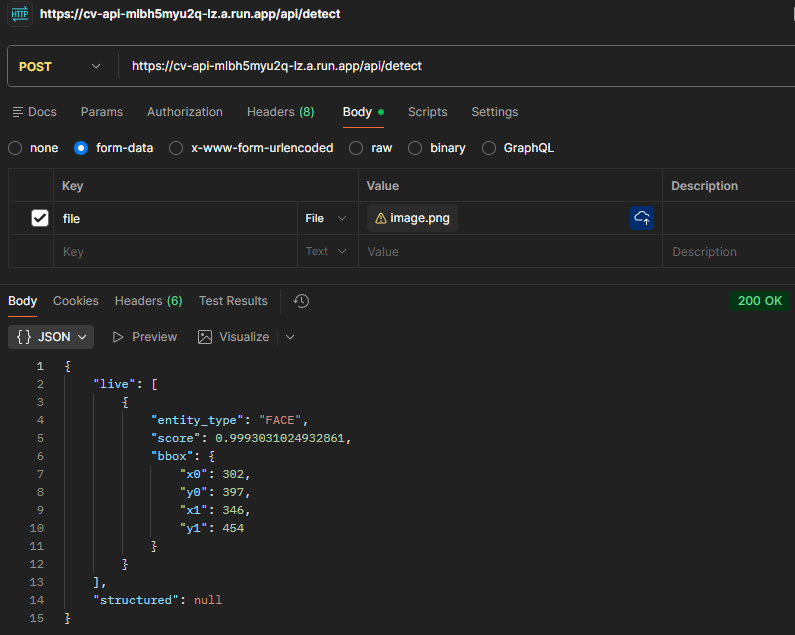
\includegraphics[width=0.80\textwidth]{figures/images/chapter-10/postman_example.png}
    \caption{Manual verification of the deployed \texttt{/api/detect} endpoint in Postman, showing multipart image upload and the returned structured JSON response.}
    \label{fig:postman_detect_backend}
\end{figure}

Coverage analysis showed strong overall backend verification. The backend reached 99\% total statement coverage, with especially high coverage in controllers, startup logic, shared processing modules, and central service layers. Several of the most important files for application behavior, including \texttt{main.py}, the controller modules, \texttt{detector\_service.py}, \texttt{frame\_live.py}, \texttt{video\_live.py}, and \texttt{pipeline\_core.py}, achieved full coverage. This indicates that the most critical backend paths for request handling, orchestration, and media processing were thoroughly exercised by the automated test suite. A complete per-file backend coverage report is provided in Appendix~\ref{appendix:backend_coverage_full}.

\begin{table}[H]
\centering
\small
\begin{tabular}{lc}
\hline
\textbf{Backend Module Group} & \textbf{Coverage} \\
\hline
Overall Backend Coverage & 96\% \\
Application Entry / Startup & 100\% \\
Controllers / API Routes & 100\% \\
Core Pipeline Modules & 100\% \\
Video Processing Core & 100\% \\
Detection Service Layer & 100\% \\
Text Analysis (PII detector) & 94\% \\
Tracking Utilities & 96--99\% \\
\hline
\end{tabular}
\caption{Summary of backend test coverage across key module groups}
\label{tab:backend_coverage}
\end{table}

Although backend coverage was high overall, the few modules with lower individual coverage were still exercised through the surrounding backend architecture. Since these components are invoked by higher level services, pipelines, and API routes, much of their practical behavior was verified indirectly through integration oriented tests. Consequently, lower isolated file coverage in these cases does not mean that the functionality was left untested, but rather that it was validated primarily as part of larger execution flows.

Overall, the backend testing process provided strong confidence in the correctness and robustness of \gls{SafeVision}'s server side functionality. The combination of route level verification, service and pipeline testing, targeted mocking of environment dependent dependencies, and manual \acrshort{api}. Verification made it possible to validate both internal logic and realistic request flows while keeping the test suite efficient and maintainable.

\section{User Testing}
\label{sec:user-testing}

User testing was conducted in multiple phases throughout the development period, with each batch corresponding to a different stage of system maturity and providing progressively more targeted insights. The initial tests, conducted in mid-March, were designed to gather both qualitative feedback on how users perceived and interacted with the system and quantitative data on usability challenges and problematic aspects. These early sessions offered a broad understanding of user behavior and highlighted key areas of difficulty. In subsequent phases, the design and execution of the tests were refined, allowing for more targeted data collection and a clearer evaluation of specific usability issues and system improvements.

\methodheading{UI Changes Based on User Testing}

Based on findings from the initial testing phases and feedback from relevant user groups (Appendix ~\ref{app:user_test_phase_1}), several changes were implemented to improve the usability and clarity of the system. The changes were aimed not only at resolving usability issues, but also at better aligning the system with practical user needs. Feedback from Skan-Kontroll emphasized that the system needed to support efficient processing, clear workflow progression, and reliable manual control over detection results. Feedback from users with image and video editing experience further highlighted the importance of predictable interaction patterns, editing precision, and clear feedback during longer processing tasks.

The most frequently observed usability issues are summarized in Table~\ref{tab:user_test_summary}. The results show that challenges related to detection feedback, workflow understanding, and navigation were among the most common problems experienced by users.

\begin{table}[h]
\centering
\begin{tabular}{lc}
\hline
\textbf{Usability Issue} & \textbf{Out of 10 Users} \\
\hline
Difficulty navigating to detection & 5 \\
Unclear detection/scanning feedback & 7 \\
Confusion about workflow steps & 6 \\
Uncertainty about system state & 4 \\
Difficulty understanding terminology & 3 \\
Issues with redaction process & 4 \\
\hline
\end{tabular}
\caption{Summary of recurring usability issues identified across initial testing phases}
\label{tab:user_test_summary}
\end{table}

In response to these findings, several interface and interaction changes were introduced. One of the main adjustments was a restructuring of the interface flow. The order of key action buttons was modified to better reflect the natural progression of tasks, making it easier for users to understand what to do next. In addition, the feature previously labeled as ``AI mission'' was renamed to ``Identify'' in order to provide clearer and more intuitive terminology, as suggested by Thomas Berg Fjellestad Appendix ~\ref{app:meeting-2026-03-17}.

To improve system feedback, loading indicators were introduced for individual files during processing. This included both the identification step and the redaction process, allowing users to better understand the current state of the system and reducing uncertainty during longer operations.

The April feedback was coded using the same recurring usability categories as the initial testing summary, making it possible to compare whether the main issues became less frequent after the interface and workflow changes. The results are summarized in Table~\ref{tab:user_test_after}. Compared with the initial testing phases, unclear detection feedback and terminology-related problems occurred less frequently, suggesting that the added progress bar and clearer terminology helped reduce some of the earlier uncertainty. However, the results also show that some challenges remained, particularly around workflow understanding and manual redaction.

\begin{table}[H]
\centering
\begin{tabular}{lc}
\hline
\textbf{Usability Issue} & \textbf{Out of 10 Users} \\
\hline
Difficulty navigating to detection & 5 \\
Unclear detection/scanning feedback & 2  \\
Confusion about workflow steps & 6 \\
Uncertainty about system state & 3  \\
Difficulty understanding terminology & 2 \\
Issues with redaction process & 6 \\
\hline
\end{tabular}
\caption{Summary of recurring usability issues identified across the April testing phase after interface and workflow improvements}
\label{tab:user_test_after}
\end{table}

The remaining issues were mainly related to users needing time to understand the first step after uploading media, as well as difficulties with editing overlapping boxes, identifying when manual tools were active, or deleting selected regions. These findings suggest that the main workflow became clearer after the implemented changes, but that progress feedback and manual editing support remained areas for further refinement. The April results therefore show improvement in several of the original problem areas, while also identifying more specific interaction issues that became visible once the basic workflow was easier to complete.


\section{Performance Tests}
\label{sec:performance_tests}

As part of the quality assurance process, performance tests were conducted to evaluate the runtime behavior of the \gls{SafeVision} system. These tests measured the latency of detection and redaction operations across different execution environments and scenario configurations. By comparing local CPU, local \gls{gpu}, and deployed cloud execution, the evaluation provides a practical view of how the system performs under different operational conditions. \Gls{inpainting} was excluded from the performance tests because the evaluation was limited to the redaction methods used most consistently in the core workflow.


\methodheading{Test Setup}

Performance was measured as total API response time per image. The reported latency therefore includes request handling, image upload, backend processing, and response generation. Detection and redaction were measured separately, using the scenario sets summarized in Table~\ref{tab:det_red_scenarios}.

\begin{table}[H]
\centering
\small
\begin{tabularx}{0.8\textwidth}{X X}
\toprule
\textbf{Detection scenarios} & \textbf{Redaction scenarios} \\
\midrule
\texttt{face\_only} & \texttt{blur\_box} \\
\texttt{text\_only} & \texttt{pixelate\_box} \\
\texttt{barcode\_only} & \texttt{blackbox\_box} \\
\texttt{license\_plate\_only} & \texttt{blur\_segmentation} \\
\texttt{object\_only} & \texttt{pixelate\_segmentation} \\
\texttt{all\_enabled} & \texttt{blackbox\_segmentation} \\
\bottomrule
\end{tabularx}


\caption{Detection and redaction scenarios included in the performance tests.}
\label{tab:det_red_scenarios}
\end{table}

For \gls{segmentation} based redaction, only \gls{segmentation} compatible detections were included. In addition, the number of \gls{segmentation} candidates was capped in order to avoid unrepresentative worst-case behavior on densely detected images. The performance measurements were collected across three execution environments, summarized in Table~\ref{tab:performance_environments}.

\begin{table}[H]
\centering
\begin{tabular}{|p{2.6cm}|p{4.3cm}|p{3.2cm}|p{4.2cm}|}
\hline
\textbf{Environment} & \textbf{Hardware / Runtime} & \textbf{Memory} & \textbf{Characteristics} \\ \hline

\textbf{Local CPU} & 
AMD Ryzen 7 5800X3D (8 cores, 16 threads) & 
32 GB RAM & 
CPU-only local execution used as the baseline environment. \\ \hline

\textbf{Local GPU} & 
NVIDIA GeForce RTX 4080 & 
16 GB dedicated \gls{gpu} memory & 
Local \gls{gpu}-accelerated execution for PyTorch-based detectors. \acrshort{ocr} remained CPU-based. \\ \hline

\textbf{Cloud} & 
Google Cloud Run (2 vCPU) & 
8 GiB memory & 
Deployed CPU-based \acrshort{api} environment with concurrency set to 1 and a minimum of 1 instance. \\ \hline

\end{tabular}
\caption{Execution environments used in the performance tests.}
\label{tab:performance_environments}
\end{table}


\methodheading{Detection Performance}

Figure~\ref{fig:detect_latency_by_environment} shows the mean detection latency across the three environments. The local \gls{gpu} environment achieved the lowest latency overall for the most computationally demanding scenarios, particularly for \texttt{face\_only} and \texttt{all\_enabled}. This indicates that the PyTorch-based detection pipelines benefited substantially from \gls{gpu} acceleration.

\begin{figure}[H]
    \centering
    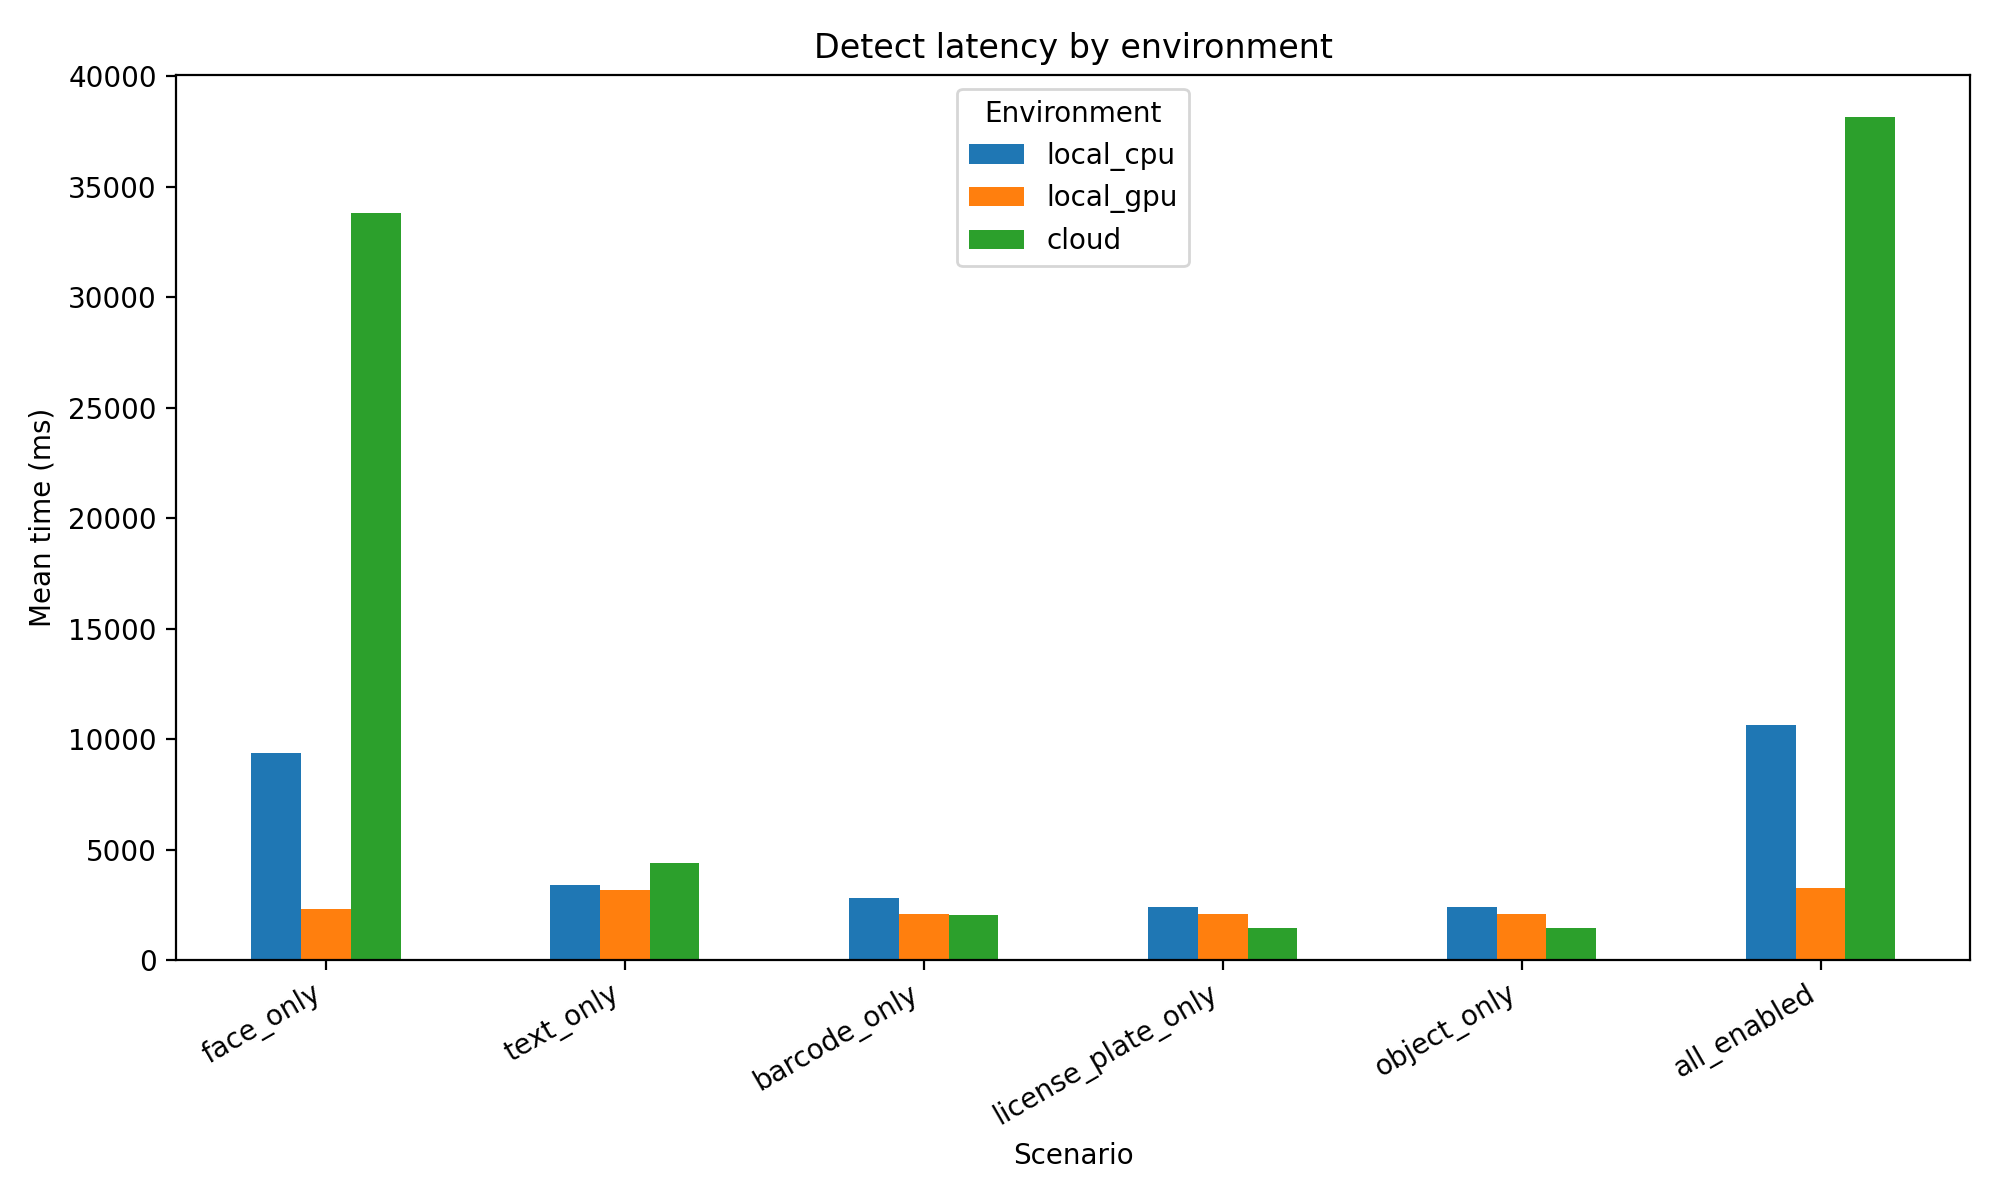
\includegraphics[width=1.1\textwidth]{figures/images/chapter-9/detect_latency_by_environment.png}
    \caption{Mean detection latency across local CPU, local \gls{gpu}, and cloud environments.}
    \label{fig:detect_latency_by_environment}
\end{figure}

The results do not, however, show a uniform ranking across all scenarios. For lighter detection tasks such as \texttt{barcode\_only},
\texttt{license\_plate\_only}, and \texttt{object\_only}, the deployed cloud environment produced lower mean latency than the local CPU environment, and in some cases also lower latency than the local \gls{gpu} environment. Since the measurements represent end-to-end \acrshort{api} response time rather than isolated model \gls{inference} time, these differences are likely influenced by a combination of runtime overhead, workload characteristics, and environment-specific execution conditions rather than hardware category alone.

For the more computationally demanding scenarios, the cloud environment showed substantially higher latency than both local environments, especially for \texttt{face\_only} and \texttt{all\_enabled}. For \texttt{text\_only}, the difference between local CPU and local \gls{gpu} was smaller, which is consistent with the \acrshort{ocr} component remaining CPU-based in the tested local \gls{gpu} configuration. \\


\methodheading{Redaction Performance}

Figure~\ref{fig:redact_latency_by_environment} shows the mean redaction latency across the three environments. For the box-based methods
(\texttt{blur\_box}, \texttt{pixelate\_box}, and \texttt{blackbox\_box}), the results were relatively similar between the local CPU and local \gls{gpu}
environments. This indicates that the redaction stage itself benefited less from \gls{gpu} acceleration than the detection stage. In these scenarios, the cloud environment produced lower mean latency than both local environments.

\begin{figure}[htbp]
    \centering
    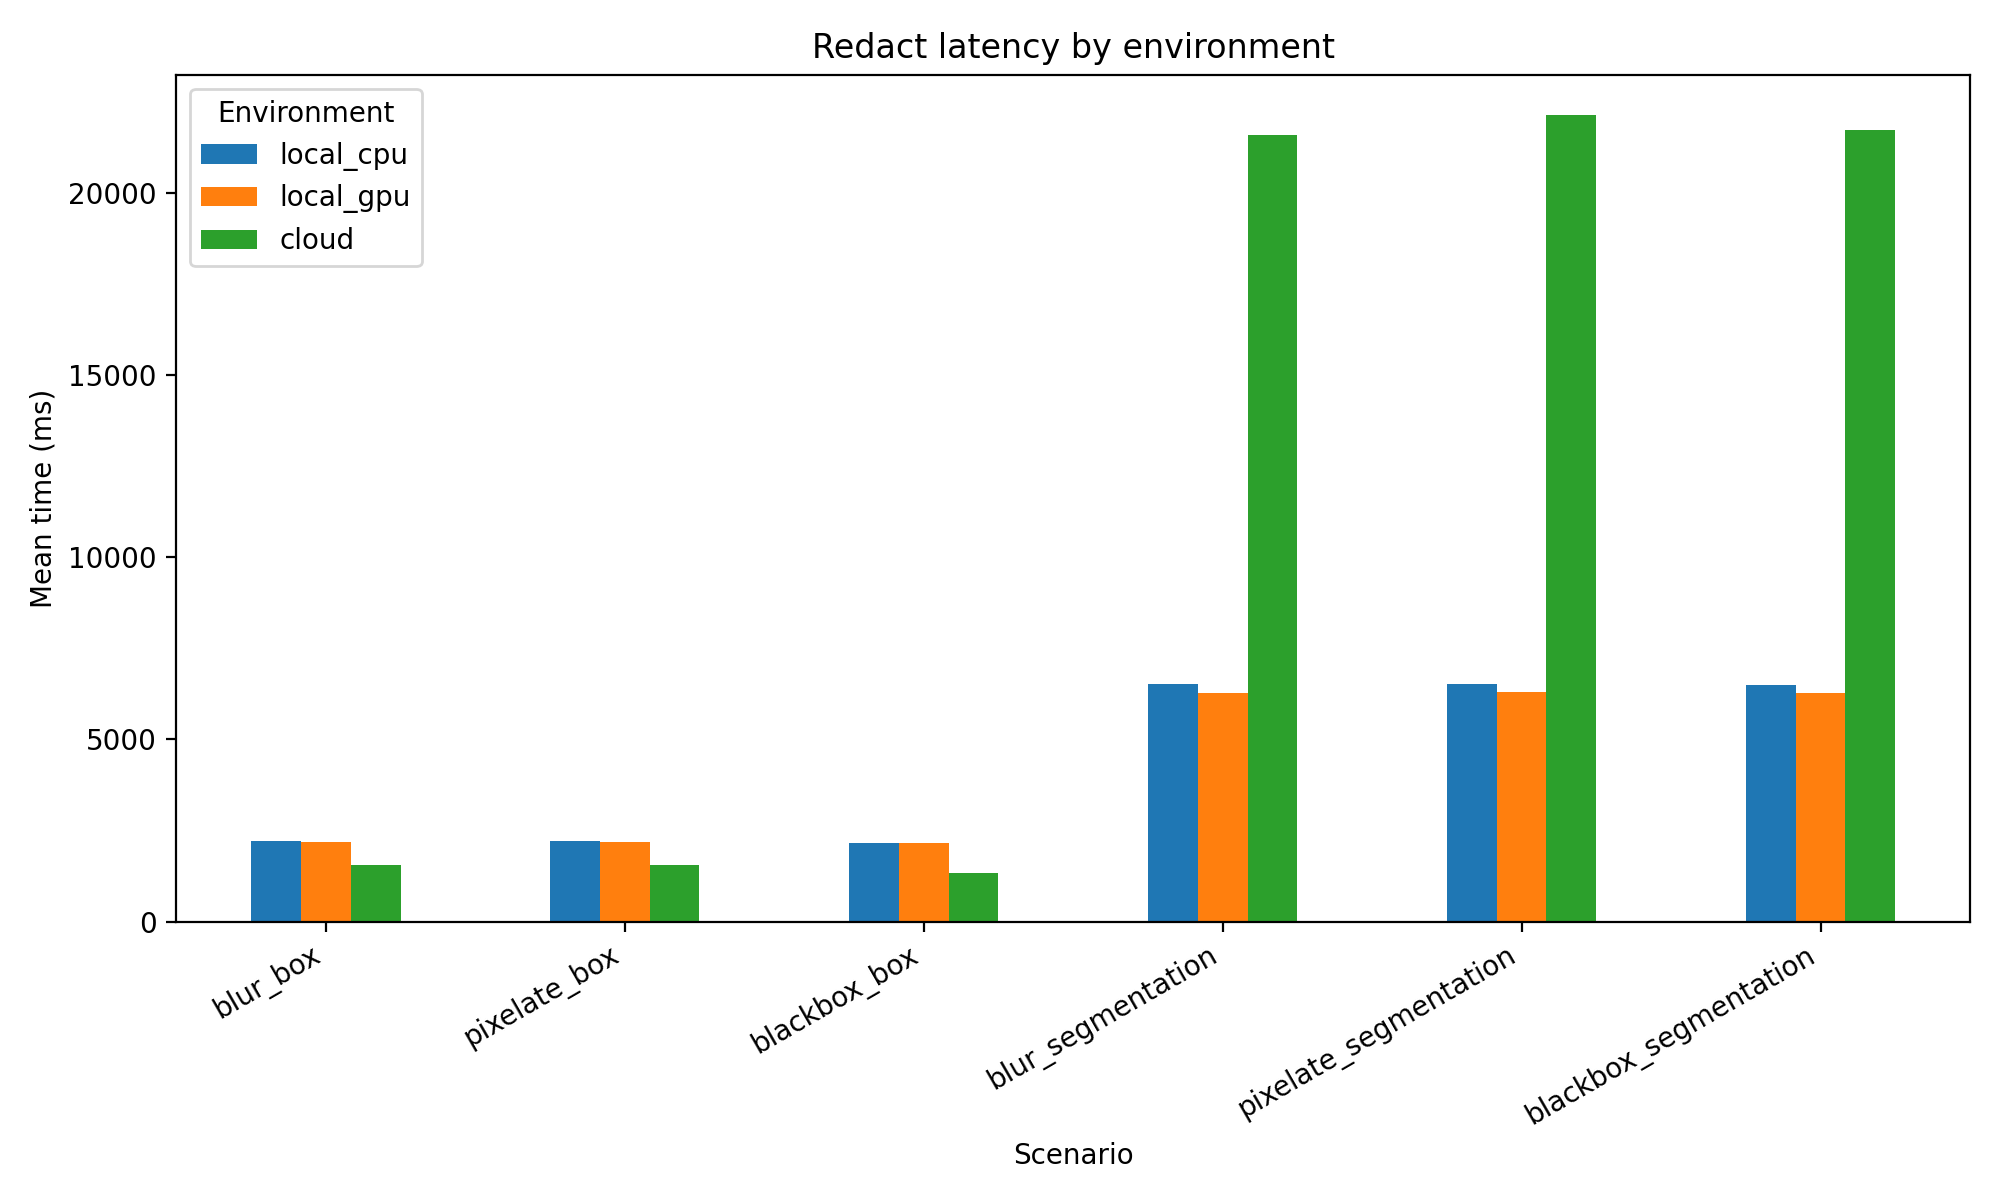
\includegraphics[width=\textwidth,height=0.38\textheight,keepaspectratio]{figures/images/chapter-9/redact_latency_by_environment.png}
    \caption{Mean redaction latency across local CPU, local \gls{gpu}, and cloud environments.}
    \label{fig:redact_latency_by_environment}
\end{figure}

For the \gls{segmentation} based methods (\texttt{blur\_segmentation}, \texttt{pixelate\_segmentation}, and \texttt{blackbox\_segmentation}), the pattern was different. In all three \gls{segmentation} scenarios, the cloud environment showed substantially higher latency than both local environments, while the local CPU and local \gls{gpu} results remained relatively close. This indicates that \gls{segmentation} based redaction introduced a much higher computational cost than box-based redaction, particularly in the deployed cloud setting.

\begin{figure}[htbp]
    \centering
    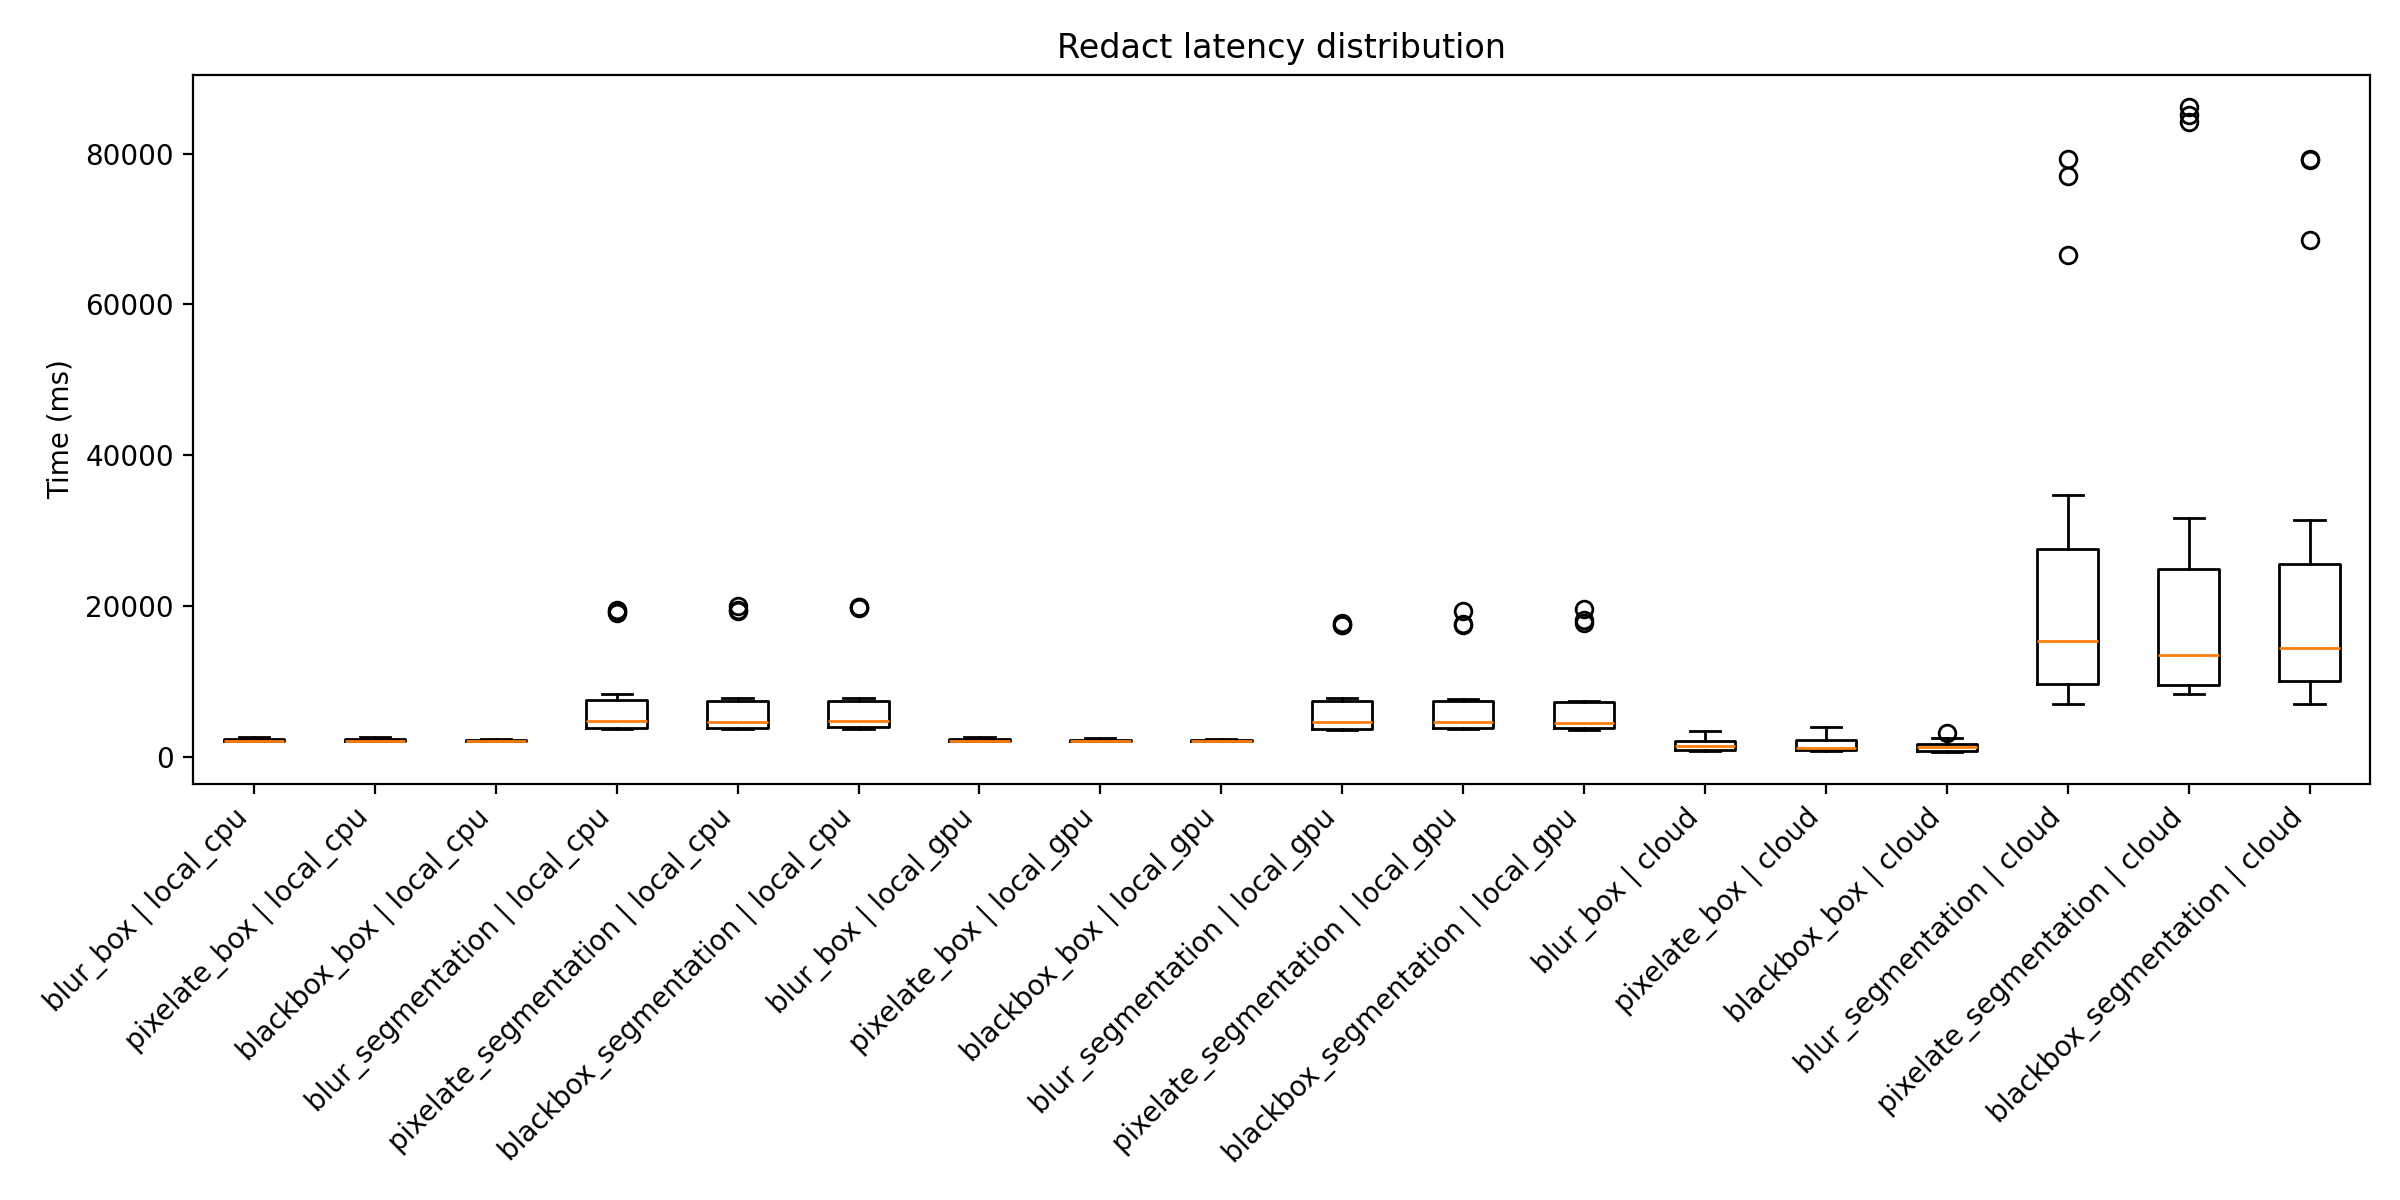
\includegraphics[width=\textwidth,height=0.40\textheight,keepaspectratio]{figures/images/chapter-9/redact_latency_distribution.png}
    \caption{Distribution of redaction latency across scenarios and environments. Lower boxes indicate faster processing, while taller boxes and longer whiskers indicate greater variation between runs. Individual points represent outliers. The cloud \gls{segmentation} scenarios show the highest latency and largest spread.}
    \label{fig:redact_latency_distribution}
\end{figure}

The difference between box-based and \gls{segmentation} based redaction is further illustrated in Figure~\ref{fig:redact_latency_distribution}, which shows that the \gls{segmentation} scenarios had both higher latency and greater variation than the box-based scenarios. This was especially visible in the cloud environment, where \gls{segmentation} based redaction produced the largest spread and the highest outlier values.

Although \gls{segmentation} based redaction was significantly slower, the average number of \gls{segmentation} compatible regions remained low and consistent across environments. This suggests that the increased latency was primarily caused by the \gls{segmentation} process itself rather than by a large number of processed regions. \\

\noindent\textbf{Discussion of Performance Results}

The results show that \gls{gpu} acceleration had the greatest effect on
detection performance, especially for the PyTorch-based detection pipelines. The effect was smaller for text detection, since \acrshort{ocr} remained CPU-based in the tested local \gls{gpu} setup. For redaction, the main distinction was not between \gls{cpu} and \gls{gpu}, but between box-based and \gls{segmentation} based methods. \Gls{segmentation} introduced a significantly higher processing cost in all environments.

The cloud-based measurements were consistently higher for the most demanding scenarios. These results should be interpreted in light of the cloud runtime configuration and the fact that the tests measured end-to-end \acrshort{api} response time rather than isolated model \gls{inference} time. The reported values therefore reflect both processing cost and deployment-related overhead.

\section{Security Evaluation}
\label{sec:security_evaluation}

The security evaluation of \gls{SafeVision} was limited to the attack surface that is relevant for the implemented prototype. The system does not include user authentication, account management, or persistent user databases, and therefore does not expose security concerns such as login bypass, session abuse, or leakage of stored user records. As a result, the evaluation addressed the parts of the system that could be tested meaningfully: \acrshort{api} robustness, malformed input handling, browser-visible data exposure, cross-origin behavior, and client-side storage practices.

The tests documented in Appendix~\ref{app:pen_test} therefore represent the most relevant practical penetration oriented evaluation for the current web application. Tests 1--15 of 19 mainly examined whether the backend handled input validation and error handling in a controlled and stable way across both valid and invalid requests. Taken together, these tests indicate that the backend generally rejects malformed or unsupported input through controlled client-side error responses rather than crashes or unstable behavior. 

Among all the penetration test, some findings are particularly important from a broader privacy and security perspective. Test 16 (Appendix~\ref{appsec:pen_test_16}.16) showed that query tampering on the \texttt{/api/detect} endpoint was handled through controlled validation errors. This suggests that the backend does not simply trust client-supplied parameters.

The browser facing findings are especially relevant in light of the privacy-by-design considerations discussed earlier in Chapter~\ref{chap:theoretical_foundation}. Visual media may contain both direct and indirect identifiers, and GDPR-related design constraints require minimizing unnecessary exposure and processing of personal data. In this context, Test 17 (Appendix~\ref{appsec:pen_test_17}.17) showed that uploaded image content was transmitted as binary form-data in the request body rather than exposed in request URLs. Operational settings such as detection parameters appeared in query strings, but the sensitive image content itself was not exposed there.

Test 18 (Appendix~\ref{appsec:pen_test_18}.18) further supports this overall picture. Normal browser use did not reveal unexpected \acrshort{cors} failures, and the backend implementation shown in Listing~\ref{lst:fastapi_routing} uses an explicit \texttt{ALLOWED\_ORIGINS} list rather than a wildcard '\texttt{*}'. Together, these observations suggest that cross-origin access is intended to be limited to expected frontend origins.

Another important result is given by Test 19 (Appendix~\ref{appsec:pen_test_19}.19), which examined client-side storage. As described earlier in Chapter~\ref{chap:technologies_and_methodologies}, \gls{SafeVision} uses browser-side storage mechanisms to support usability and reduce unnecessary server-side persistence. The inspection showed mainly user preferences and workflow related state, which is a positive finding from a privacy perspective, although locally stored data may still remain accessible on the client device. A summary of the most relevant findings is shown in Table~\ref{tab:security_summary}.

\begin{table}[H]
\centering
\small
\begin{tabularx}{\textwidth}{|p{1.5cm}|p{4.4cm}|X|}
\hline
\textbf{Test} & \textbf{Area} & \textbf{Key finding} \\ \hline

\textbf{16} & 
Input validation & 
Query tampering attempts were rejected safely through controlled validation errors. \\ \hline

\textbf{17} & 
Network exposure & 
Sensitive image content was not exposed in request URLs. \\ \hline

\textbf{18} & 
CORS & 
Cross-origin behavior appeared restricted to expected frontend origins. \\ \hline

\textbf{19} & 
Client-side storage & 
Stored browser data mainly consisted of preferences and workflow-related state. \\ \hline

\end{tabularx}
\caption{Key findings from the security evaluation.}
\label{tab:security_summary}
\end{table}

These findings suggest that \gls{SafeVision} follows a practical privacy conscious design. The system handles malformed \acrshort{api} input in a controlled way, does not appear to expose sensitive visual content unnecessarily in URLs, and relies on browser-side storage rather than avoidable server-side persistence. Within its current scope, the system therefore appears reasonably robust and privacy aware.






\section{Irreversibility Verification of Exported Redactions}
\label{sec:irreversibility-verification}

A central security property of \gls{SafeVision} is that exported redacted images must not retain the original pixel content within the redacted region. This section evaluates whether the black box redaction method satisfies this requirement at the pixel level, that is, whether the export process performs a destructive overwrite of the selected region rather than a visual overlay. Although black box redaction is used as the representative example, the underlying principle applies to all redaction methods supported by the system. The mathematical basis for the irreversibility argument and the complete verification script are provided in Appendix~\ref{app:redaction_irreversibility}.

\methodheading{Verification Approach}

A redaction method is privacy preserving in the exported file only if the original pixel values within the redacted region are no longer recoverable from that file alone. To verify this for \gls{SafeVision}, the analysis examined whether the downloaded 
image retained the original pixel data inside the detected region or whether those values had been replaced during export. The evaluation was performed on an image processed through the full \gls{SafeVision} pipeline, including detection, user confirmation, and export.

As \gls{SafeVision} resizes images during export, the coordinate space changes between the original and exported image. The detected region coordinates returned by the backend were therefore scaled to match the exported image before the pixel-level analysis was applied. The original image had a resolution of $4928 \times 3008$ pixels, and the exported redacted image had a resolution of $1400 \times 855$ pixels. The scale factors in the horizontal and vertical directions were 0.2841 and 0.2842, respectively, indicating near-uniform scaling. The original detection region was:
\[
R_{\text{original}} = (823,\; 499,\; 2562,\; 2950),
\]
which, after scaling to the exported image resolution, became:
\[
R_{\text{exported}} = (234,\; 142,\; 728,\; 839),
\]
corresponding to a region of $494 \times 697$ pixels, totalling 344,318 pixels.

The verification evaluated two properties over this region. First, it measured the proportion of pixels in the exported region that were black or near-black, using a tolerance of 15 intensity levels to account for minor differences introduced by down scaling, anti-aliasing, or encoding. Second, it measured the proportion of pixels that differed from the corresponding region in the original image. A threshold of 99\% was applied to both properties, reflecting the 
expectation that a small number of boundary pixels may be affected by scaling artifacts without compromising the integrity of the redaction.

\methodheading{Visual Verification and Results}

Figure~\ref{fig:org_vs_redaction} illustrates the effect of black box redaction on the exported image. The detected region $R$ is outlined prior to redaction and shown replaced by black pixels in the exported file, providing visual confirmation that the content within the region is no longer present. This is further supported by the pixel-level results summarized in Table~\ref{tab:redaction-irreversibility-results}.

\begin{figure}[H]
\centering
\begin{subfigure}{0.48\textwidth}
    \centering
    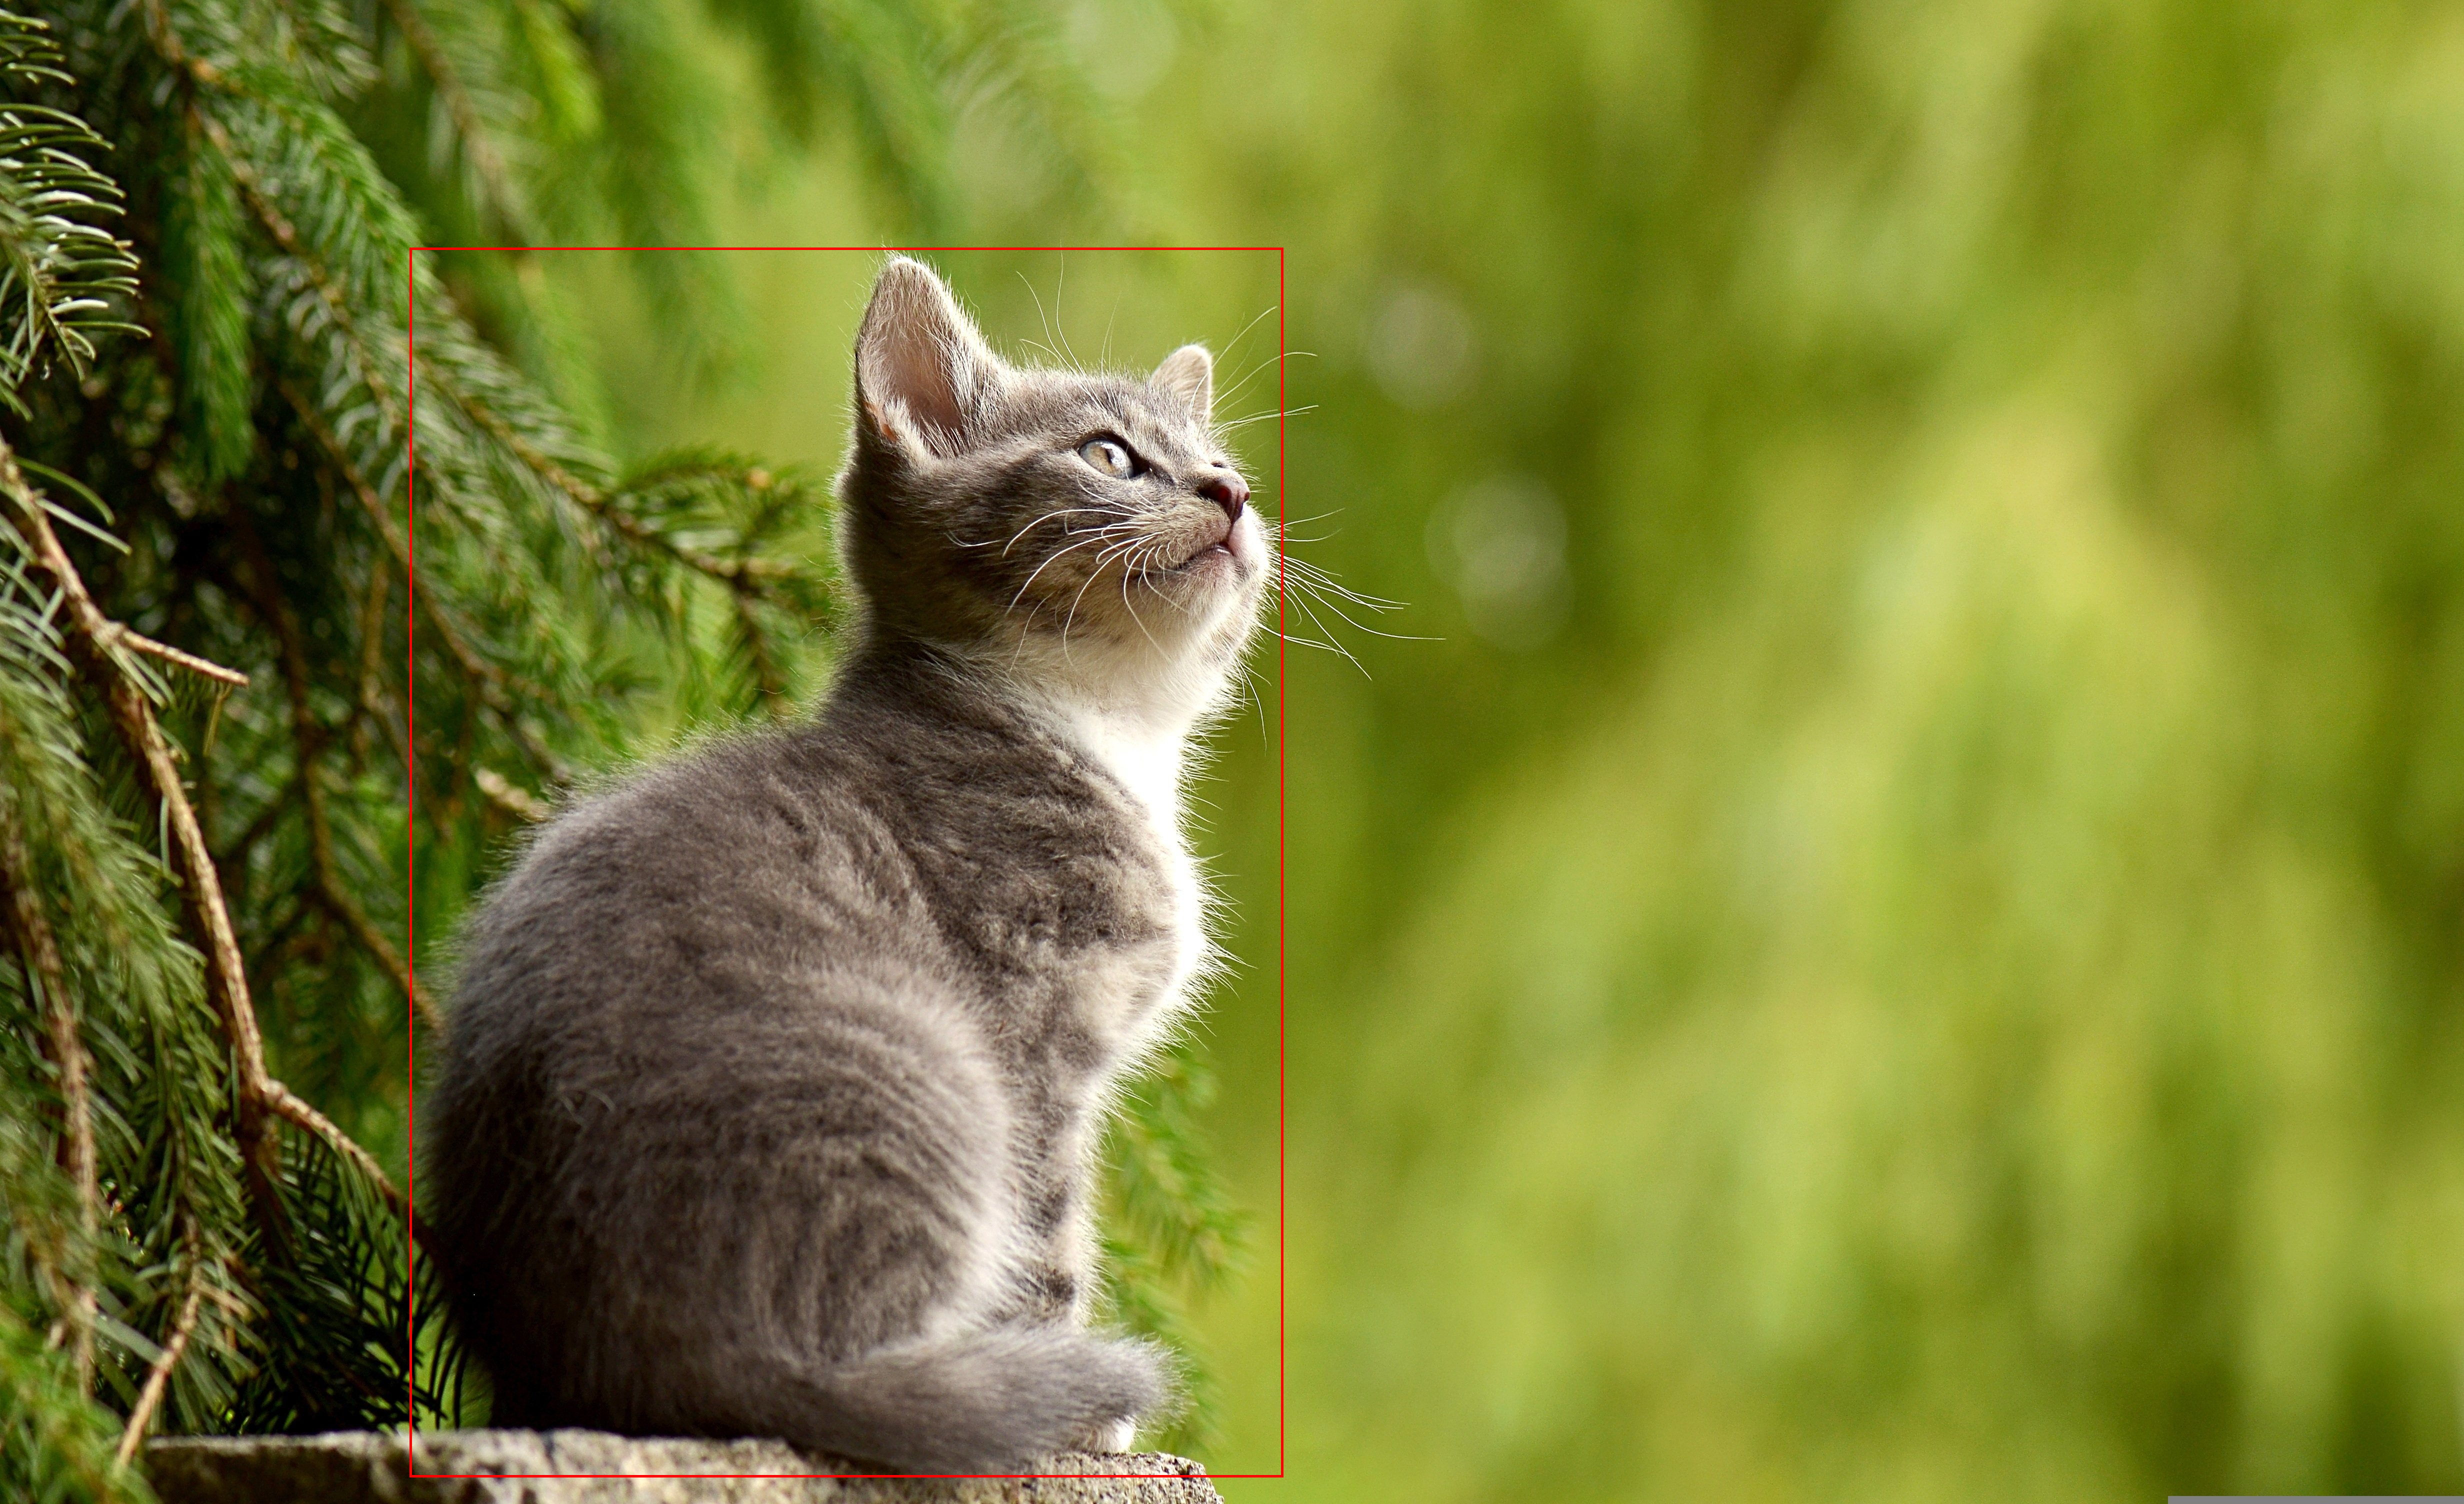
\includegraphics[width=\textwidth]{figures/images/chapter-9/figure_1_original_with_region.png}
    \caption{Original image with the detected region $R$ marked prior to redaction.}
\end{subfigure}
\hfill
\begin{subfigure}{0.48\textwidth}
    \centering
    
\includegraphics[width=\textwidth]{figures/images/chapter-9/figure_2_redacted_with_region.png}
    \caption{Exported image after redaction, with $R$ scaled to the exported resolution.}
\end{subfigure}
\caption{Comparison of the original and exported redacted image, showing that the 
content within $R$ has been replaced by black pixels. Image source: 
\cite{pixabay_cat_2083492}.}
\label{fig:org_vs_redaction}
\end{figure}

\begin{table}[H]
\centering
\caption{Pixel-level verification results for exported black box redaction.}
\label{tab:redaction-irreversibility-results}
\begin{tabular}{l r}
\toprule
\textbf{Metric} & \textbf{Result} \\
\midrule
Original image size                    & $4928 \times 3008$ \\
Exported image size                    & $1400 \times 855$ \\
Scale factor in x-direction            & 0.2841 \\
Scale factor in y-direction            & 0.2842 \\
Original region coordinates            & $(823,\; 499,\; 2562,\; 2950)$ \\
Scaled exported region coordinates     & $(234,\; 142,\; 728,\; 839)$ \\
Analysed region size                   & $494 \times 697$ pixels \\
Total analysed pixels                  & 344,318 \\
Black or near-black pixels             & 99.857\% \\
Changed pixels compared with original & 99.945\% \\
Metadata in exported PNG               & No EXIF data found \\
Test result                            & Passed \\
\bottomrule
\end{tabular}
\end{table}

Of the 344,318 pixels in the analysed region, 99.857\% were black or near-black within the defined tolerance, and 99.945\% differed from the corresponding pixels in the original image, both exceeding the 99\% threshold. The small proportion of pixels that did not satisfy both criteria is consistent with boundary effects at the edge of the redacted region, where downscaling and anti-aliasing can produce intermediate values. The exported PNG contained no EXIF metadata, indicating that image metadata was not retained during export.

\methodheading{Interpretation and Limitations}

The results confirm that black box redaction in \gls{SafeVision} is destructive at the pixel level in the exported image. The redacted region is not rendered as a visual overlay within the \acrshort{ui} but is instead exported as overwritten pixel data, such that an adversary with access only to the downloaded file cannot recover 
the original content from it. Among the redaction methods supported by the system, black box and solid fill provide the strongest irreversibility guarantees, since they replace original pixel values with a constant. Methods such as blur and pixelation are lossy transformations that derive their output from the original pixels and may preserve partial visual information; these should accordingly be considered weaker from a privacy perspective.

This conclusion is subject to the conditions under which the evaluation was conducted. It applies specifically to the exported redacted file and assumes that an adversary does not have access to the original uploaded image, server-side copies, browser cache, backups, or other external sources that may retain the original data. It is also important to note that irreversibility is a
property of the export process rather than of detection or \gls{segmentation}: those components identify the region $R$, but it is the destructive pixel overwrite during export that establishes the security guarantee evaluated here.






\afterpage{\blankpage}


\chapter{Sustainability Analysis}

\section{Sustainability Assessment Framework}

The sustainability of the SafeVision system is evaluated using the Sustainability Awareness Framework (SusAF), which provides a structured approach for analyzing software systems across multiple dimensions and time horizons. The framework considers five dimensions of sustainability: human, social, environmental, economic, and technical. In addition, it distinguishes between three levels of effects: immediate, enabling, and structural \cite{penzenstadler2013sustainability}.

Immediate effects refer to the direct impact of the system during use. Enabling effects describe how the system influences user behavior and workflows, while structural effects capture long term consequences for organizations and society. This perspective allows the evaluation to go beyond technical performance and consider broader implications of deploying SafeVision.

\begin{figure}[H]
\centering
\resizebox{\textwidth}{!}{%
\begin{tikzpicture}[x=1cm,y=1cm]

% -------------------------------------------------
% GEOMETRY
% -------------------------------------------------
\def\rI{3.3}    % Immediate boundary
\def\rE{5.6}    % Enabling boundary
\def\rS{8.2}    % Structural boundary

% Pentagon angles
\def\aTop{90}
\def\aUR{18}
\def\aLR{-54}
\def\aLL{-126}
\def\aUL{162}

% -------------------------------------------------
% STYLES
% -------------------------------------------------
\tikzset{
  posbox/.style={
    fill=green!70,
    draw=none,
    rounded corners=1.5pt,
    align=center,
    text width=2.65cm,
    inner sep=3pt,
    font=\scriptsize
  },
  negbox/.style={
    fill=orange!85,
    draw=none,
    rounded corners=1.5pt,
    align=center,
    text width=2.65cm,
    inner sep=3pt,
    font=\scriptsize
  },
  arrow/.style={
    -{Latex[length=2.2mm]},
    thick
  },
  levellabel/.style={
    font=\scriptsize,
    fill=white,
    fill opacity=0.90,
    text opacity=1,
    inner sep=1.5pt
  }
}

% -------------------------------------------------
% BACKGROUND PENTAGONS
% -------------------------------------------------
\fill[blue!28]
  (\aTop:\rS) -- (\aUR:\rS) -- (\aLR:\rS) -- (\aLL:\rS) -- (\aUL:\rS) -- cycle;

\fill[blue!18]
  (\aTop:\rE) -- (\aUR:\rE) -- (\aLR:\rE) -- (\aLL:\rE) -- (\aUL:\rE) -- cycle;

\fill[blue!8]
  (\aTop:\rI) -- (\aUR:\rI) -- (\aLR:\rI) -- (\aLL:\rI) -- (\aUL:\rI) -- cycle;

% -------------------------------------------------
% RADIAL LINES
% -------------------------------------------------
\draw[thick] (0,0) -- (\aTop:\rS);
\draw[thick] (0,0) -- (\aUR:\rS);
\draw[thick] (0,0) -- (\aLR:\rS);
\draw[thick] (0,0) -- (\aLL:\rS);
\draw[thick] (0,0) -- (\aUL:\rS);

% -------------------------------------------------
% CENTER
% -------------------------------------------------
\fill[pink!60] (0,0) ellipse (1.18 and 0.72);
\node[font=\bfseries\small] at (0,0) {SafeVision};

% -------------------------------------------------
% OUTER DIMENSION LABELS
% -------------------------------------------------
\node[font=\bfseries\small, rotate=35]  at (145:8.95) {Social};
\node[font=\bfseries\small, rotate=-35] at (35:8.95)  {Individual};
\node[font=\bfseries\small, rotate=-74] at (342:9.05) {Technical};
\node[font=\bfseries\small]             at (270:9.15) {Economic};
\node[font=\bfseries\small, rotate=74]  at (198:9.05) {Environmental};

% -------------------------------------------------
% LEVEL LABELS
% -------------------------------------------------
\node[levellabel] at (2.45,-1.65) {Immediate};
\node[levellabel] at (2.85,-4.15) {Enabling};
\node[levellabel] at (3.15,-6.35) {Structural};

% -------------------------------------------------
% IMPACT BOXES
% Top four intentionally placed in the enabling ring
% -------------------------------------------------

% Social / Individual (top four in enabling ring)
\node[posbox, rotate=24] (SI1) at (-1.85,3.55)
{SI1\\Improved privacy\\protection (+)};

\node[posbox, rotate=18] (SE1) at (-4.20,2.00)
{SE1\\Standardized privacy\\workflows (+)};

\node[posbox, rotate=-24] (II1) at (1.85,3.55)
{II1\\Faster redaction\\and review (+)};

\node[posbox, rotate=-18] (IE1) at (4.15,2.00)
{IE1\\Non-expert\\redaction use (+)};

% Technical
\node[posbox, rotate=-30] (TI1) at (4.20,-1.20)
{TI1\\Modular system\\architecture (+)};

\node[negbox, rotate=-30] (TS1) at (5.00,-4.05)
{TS1\\Model drift and\\testing effort (-)};

% Environmental
\node[negbox, rotate=28] (EnI1) at (-2.55,-1.55)
{EnI1\\Inference energy\\use (-)};

\node[posbox, rotate=14] (EnE1) at (-5.35,-3.15)
{EnE1\\Less storage and\\data transfer (+)};

\node[negbox] (EnS1) at (-4.35,-5.45)
{EnS1\\Rebound effect\\from higher use (-)};

% Economic
\node[posbox] (EcI1) at (0.00,-2.45)
{EcI1\\Lower labor\\cost (+)};

\node[posbox] (EcE1) at (0.00,-4.25)
{EcE1\\Scalable processing\\workflows (+)};

\node[negbox] (EcS1) at (0.00,-6.05)
{EcS1\\Maintenance and\\model update costs (-)};

% -------------------------------------------------
% ARROWS
% Reduced to the most important dependencies
% -------------------------------------------------

% Social
\draw[arrow] (SI1.north west) to[out=-150,in=85] (SE1.north);

% Individual to economic
\draw[arrow] (II1.south) to[out=-88,in=70] (EcI1.north east);

% Technical
\draw[arrow] (TI1.south east) to[out=-40,in=90] (TS1.north);

% Environmental
\draw[arrow] (EnI1.south) to[out=-105,in=85] (EnS1.north);
\draw[arrow] (EnE1.south) to[out=-95,in=165] (EnS1.north west);

% Economic chain
\draw[arrow] (EcI1.south) -- (EcE1.north);
\draw[arrow] (EcE1.south) -- (EcS1.north);

\end{tikzpicture}%
}
\caption{SusAF model for SafeVision. Created by the authors, with AI-assisted refinement.}
\label{fig:susaf-safevision}
\end{figure}

The SusAF model shows that SafeVision has mainly positive sustainability effects in the social, individual, economic, and technical dimensions. The system supports improved privacy protection, faster redaction work, more standardized workflows, and lower labor costs, while its modular architecture contributes positively to technical sustainability. At the same time, the model highlights important trade-offs. Machine learning inference increases energy consumption, and long-term use may contribute to rebound effects, model drift, testing effort, and recurring maintenance costs.

%------------------------- HUMAN ---------------------------

\section{Human Dimension}

\noindent\textbf{Immediate Effects}

SafeVision improves user efficiency by automating the detection of sensitive information in images. Manual identification of such content is time consuming and cognitively demanding, particularly when working with large datasets or under time constraints.

Automation reduces repetitive tasks and allows users to focus on higher level decision making, such as validating and refining detection results. Studies indicate that automation can improve productivity in data intensive tasks by up to 20--40\% by reducing manual effort and cognitive load \cite{bessen2019ai}.

In SafeVision, this means that users no longer need to manually scan entire images for sensitive content. Instead, they review pre identified regions, which significantly reduces the time required per image. For example, when processing large collections of media content, automated detection can reduce inspection time from minutes to seconds per image.

However, this shift introduces a dependency on system accuracy. Research shows that users interacting with automated systems may experience reduced attention and increased trust in system outputs, which can lead to overlooked errors if validation is insufficient \cite{parasuraman1997humans}. This creates a trade off between efficiency and vigilance.

\noindent\textbf{Enabling Effects}

SafeVision enables more structured and consistent handling of sensitive data by integrating detection and redaction into a single workflow. This reduces variability in how tasks are performed and promotes standardized practices.

This is particularly relevant in the context of the General Data Protection Regulation, which imposes strict requirements on the processing of personal data \cite{voigt2017gdpr}. Manual compliance with such regulations can be complex and error prone. By embedding privacy preserving mechanisms directly into the system, SafeVision reduces the likelihood of incorrect data handling.

The system also lowers the barrier for non expert users. Individuals without specialized training can perform redaction tasks through an intuitive interface. While this improves accessibility, it may also introduce inconsistencies if users interpret detection results differently or apply redaction in varying ways.

\noindent\textbf{Structural Effects}

In the long term, systems like SafeVision may influence organizational practices related to privacy and data protection. Increased adoption of automated tools can lead to more consistent anonymization standards and greater awareness of privacy risks.

At the same time, there is a risk of over reliance on automation. If users assume that detection is always correct, errors may propagate unnoticed. This is particularly critical in privacy sensitive contexts where missed detections can lead to exposure of personal data.

Maintaining a human in the loop approach is therefore essential. Research emphasizes that effective human AI collaboration requires balancing automation with user control and transparency \cite{amershi2019guidelines}. SafeVision reflects this by allowing users to validate and adjust results before redaction is applied.

%------------------------- SOCIAL ---------------------------

\section{Social Dimension}

\noindent\textbf{Immediate Effects}

SafeVision contributes to improved privacy protection by reducing the likelihood that sensitive personal information is unintentionally exposed in shared media. By assisting users in identifying and redacting personal data, the system supports safer handling of digital content and may increase trust in data sharing workflows, particularly in environments where images and videos are regularly processed for documentation, communication, or analysis \cite{li2024image,zhao2023visual}. More reliable anonymization can reduce concerns related to accidental privacy breaches and improve confidence in privacy-sensitive digital workflows \cite{gdpr2016}.

However, trust in automated privacy tools must be balanced with transparency and user awareness. If users do not understand the limitations of detection models, they may place excessive confidence in system output, which can create false perceptions of safety and increase the risk that undetected sensitive information is overlooked \cite{parasuraman1997humans,amershi2019guidelines}. Long-term effectiveness therefore depends not only on automation accuracy, but also on maintaining informed human oversight during validation and redaction.

\noindent\textbf{Enabling Effects}

At an organizational level, SafeVision enables more consistent privacy-preserving workflows by embedding anonymization directly into digital processing pipelines. This supports compliance-oriented practices, reduces variation in how sensitive data is handled across users or departments, and improves accessibility by allowing non-expert users to perform privacy protection tasks without requiring specialized technical knowledge \cite{voigt2017gdpr,becker2015requirements}. As a result, a broader range of users can safely manage privacy-sensitive material within structured workflows.

At the same time, increased adoption of automated systems may create dependency on specific technical solutions, potentially reducing awareness of underlying privacy risks and the continued importance of human validation \cite{amershi2019guidelines}. If privacy protection becomes viewed primarily as an automated process, organizations may place too much trust in technical safeguards alone, weakening critical review practices that remain necessary when handling sensitive information.

\noindent\textbf{Structural Effects}

In the long term, systems like SafeVision may contribute to broader societal expectations that privacy protection should be integrated by design into digital tools and workflows. This aligns with principles such as privacy by design and growing regulatory expectations surrounding responsible data processing \cite{gdpr2016,voigt2017gdpr}. Widespread adoption of automated anonymization tools may also strengthen organizational privacy culture by making privacy-preserving practices more routine, scalable, and consistently integrated into everyday digital operations \cite{becker2015requirements}.

However, increasing societal reliance on automated privacy tools introduces risks if such systems are deployed without sufficient transparency, accountability, or oversight. Over time, excessive dependence on automation may weaken critical human review practices and create false assumptions that technical safeguards alone are sufficient \cite{parasuraman1997humans,amershi2019guidelines}. Long-term social sustainability therefore depends on maintaining user understanding, organizational responsibility, and meaningful human oversight in privacy-critical workflows.

%------------------------- ENVIRONMENTAL ---------------------------

\section{Environmental Dimension}

\noindent\textbf{Immediate Effects}

The environmental impact of SafeVision is primarily related to computational resource usage during image processing. Machine learning tasks such as object detection and segmentation require significant processing power, particularly for high resolution images.

The ICT sector is estimated to contribute between 2\% and 4\% of global carbon emissions \cite{malmodin2018ict}, while data centers account for approximately 1\% to 1.5\% of global electricity consumption \cite{iea2023datacenters}. Although SafeVision operates at a smaller scale, its reliance on machine learning models contributes to this broader impact.

Research has shown that training large machine learning models can produce substantial emissions, in some cases exceeding several hundred kilograms of CO$_2$ \cite{strubell2019energy}. SafeVision primarily uses pre trained models and focuses on inference, which is less energy intensive. However, repeated inference at scale can still result in significant cumulative energy consumption.

To reduce this impact, SafeVision processes data on demand and avoids persistent storage of images on the server. This limits unnecessary resource usage and reduces long term storage costs.

\noindent\textbf{Enabling Effects}

Automation reduces the need for repeated manual processing of the same data. In traditional workflows, images may be reviewed multiple times by different users, leading to inefficiencies.

By streamlining detection and redaction, SafeVision reduces the number of operations required per task. In addition, the use of client side storage reduces server load and minimizes data transfer, which can lower energy consumption associated with network communication.

However, these improvements may be offset by increased usage. As the system becomes faster and easier to use, users may process larger volumes of data. This phenomenon, often referred to as the rebound effect, can lead to increased total energy consumption despite improved efficiency per task \cite{hilty2011rebound}.

\noindent\textbf{Structural Effects}

At a larger scale, the adoption of systems like SafeVision may contribute to more efficient digital workflows and improved resource utilization across organizations.

At the same time, the increasing use of machine learning technologies raises concerns about growing computational demand. Studies indicate that global data traffic and processing requirements continue to increase rapidly, driven in part by AI applications \cite{andrae2015global}.

This creates a fundamental trade off. While individual systems may become more efficient, widespread adoption can increase total energy consumption. Long term sustainability therefore depends on both efficient system design and responsible usage patterns.

%------------------------- ECONOMIC ---------------------------

\section{Economic Dimension}

\noindent\textbf{Immediate Effects}

SafeVision reduces the time required to perform redaction tasks, leading to lower operational costs. Manual redaction is labor intensive and often requires trained personnel, especially when processing large volumes of images.

Automation can significantly reduce time spent on repetitive tasks. Studies show that AI supported workflows can improve productivity by up to 20--40\% in data processing contexts \cite{bessen2019ai}. When applied at scale, even small improvements can lead to substantial cost savings.

In SafeVision, this translates to reduced labor costs and faster processing times. However, these benefits depend on system accuracy. Incorrect detections may require reprocessing, which can reduce efficiency gains.

\noindent\textbf{Enabling Effects}

The system enables organizations to handle larger workloads without proportional increases in staffing. This improves productivity and allows human resources to focus on more complex tasks.

The modular and API based design also reduces integration costs. SafeVision can be incorporated into existing workflows without extensive restructuring, which lowers adoption barriers.

However, organizations must consider initial implementation costs, including infrastructure, training, and system integration. These upfront investments may be significant, particularly for smaller organizations.

\noindent\textbf{Structural Effects}

In the long term, automated redaction systems may transform how organizations manage sensitive data by enabling scalable and standardized workflows.

Industry reports indicate that a large proportion of organizations are investing in artificial intelligence to improve efficiency and reduce costs \cite{mckinsey2021ai}. Systems like SafeVision align with this trend by supporting automation in data processing tasks.

At the same time, long term economic sustainability depends on ongoing maintenance, including model updates and system monitoring. Machine learning systems require continuous evaluation to maintain accuracy, which introduces recurring costs.

In addition, increased reliance on automation may shift workforce requirements, requiring new skills related to system operation and validation.

%------------------------- TECHNICAL ---------------------------

\section{Technical Dimension}

\noindent\textbf{Immediate Effects}

SafeVision introduces technical complexity through the integration of multiple machine learning models and interactive frontend components. These components must operate together within a unified processing pipeline.

This complexity is managed through a modular architecture that separates concerns between components. This improves maintainability by allowing individual modules to be updated or replaced independently.

The stateless backend design further improves scalability and reliability. Stateless systems are easier to scale horizontally and reduce the risk of system wide failures \cite{fielding2000rest}.

\noindent\textbf{Enabling Effects}

The modular design enables continuous improvement and adaptability. New detection models can be integrated without affecting other parts of the system, allowing SafeVision to evolve alongside advances in machine learning.

The use of standardized APIs improves interoperability and supports integration with other systems. This aligns with principles of sustainable software engineering, which emphasize adaptability and reuse \cite{becker2015requirements}.

However, modular systems also introduce coordination challenges. Ensuring compatibility between components requires careful design, testing, and version management.

\noindent\textbf{Structural Effects}

From a long term perspective, SafeVision supports sustainable software development through modularity, scalability, and adaptability. These characteristics enable the system to evolve without requiring complete redesign.

Research highlights that maintainability and adaptability are key factors in long term software sustainability \cite{venters2014software}. SafeVision reflects these principles through its separation of detection, redaction, and interface components.

At the same time, machine learning systems introduce additional challenges such as model drift, where performance degrades as data changes over time. Addressing this requires continuous monitoring and periodic updates.

Increased system complexity can also make debugging and testing more difficult. Ensuring long term reliability therefore depends on robust testing strategies and clear system boundaries.

\chapter{Results}
\label{chap:results}

This chapter presents the main results from the implemented \gls{SafeVision} system. The evaluation covers both pre-trained models integrated into the \gls{anonymization} pipeline and custom-trained models developed during the project. In addition, the chapter reports results from the video processing extension, including qualitative redaction examples, manual tracking accuracy, prediction-based frame coverage, and processing performance.

%------------------------11.1-------------------------

\section{Pre-Trained Model Results}

This chapter presents the results obtained using pre-trained models integrated into the \gls{anonymization} pipeline. The models were used without additional fine-tuning and evaluated directly within the full system. To provide context for the observed performance, benchmark results from the original implementations are included alongside qualitative and system-level observations.

\methodheading{Face Detection}

Face detection was performed using the pre-trained RetinaFace model through the PyTorch implementation provided by \texttt{biubug6/Pytorch\_Retinaface} \cite{biubug6_retinaface}.  Table~\ref{tab:retinaface_widerface} summarizes the reported validation performance on the WIDER FACE dataset using single-scale evaluation. The implementation provides results for both \texttt{ResNet50} and \texttt{MobileNet0.25} backbones. The \texttt{ResNet50} backbone achieves the strongest reported performance, with 94.82\%, 93.84\%, and 89.60\% on the easy, medium, and hard subsets, respectively, while the lightweight \texttt{MobileNet0.25} configuration achieves 88.67\%, 87.09\%, and 80.99\%.

\begin{table}[H]
\centering
\begin{tabular}{lccc}
\toprule
Backbone / Style & Easy & Medium & Hard \\
\midrule
ResNet50 (PyTorch, same parameters as MxNet) & 94.82\% & 93.84\% & 89.60\% \\
MobileNet0.25 (PyTorch, same parameters as MxNet) & 88.67\% & 87.09\% & 80.99\% \\
\bottomrule
\end{tabular}
\caption{Reported WIDER FACE validation performance of the RetinaFace PyTorch implementation using single-scale evaluation \cite{biubug6_retinaface}.}
\label{tab:retinaface_widerface}
\end{table}

These benchmark results provide context for the observed system performance, where RetinaFace produced stable and consistent face detections across a wide range of input images. In practice, the model was able to accurately localize faces under varying lighting conditions and moderate occlusions, and it maintained high detection confidence for most visible faces.

The precision--recall curves reported for the WIDER FACE validation set are shown in Figure~\ref{fig:retinaface_widerface_combined}. The curves illustrate the expected decrease in performance as the evaluation setting becomes more challenging. This trend was also reflected in the system, where detection performance was slightly reduced for small or heavily occluded faces, while remaining strong for clearly visible faces.

The precision--recall curves reported for the WIDER FACE validation set are shown in Figure~\ref{fig:retinaface_widerface_combined}. The figure is included as benchmark context and shows RetinaFace compared with other face detection methods on the easy, medium, and hard subsets of WIDER FACE. It does not distinguish between the \texttt{ResNet50} and \texttt{MobileNet0.25} backbones used in the PyTorch implementation; these backbone-specific results are instead reported in Table~\ref{tab:retinaface_widerface}. Overall, the curves show that RetinaFace performs competitively on WIDER FACE, while performance decreases as the evaluation subset becomes more challenging.

\begin{figure}[H]
\centering
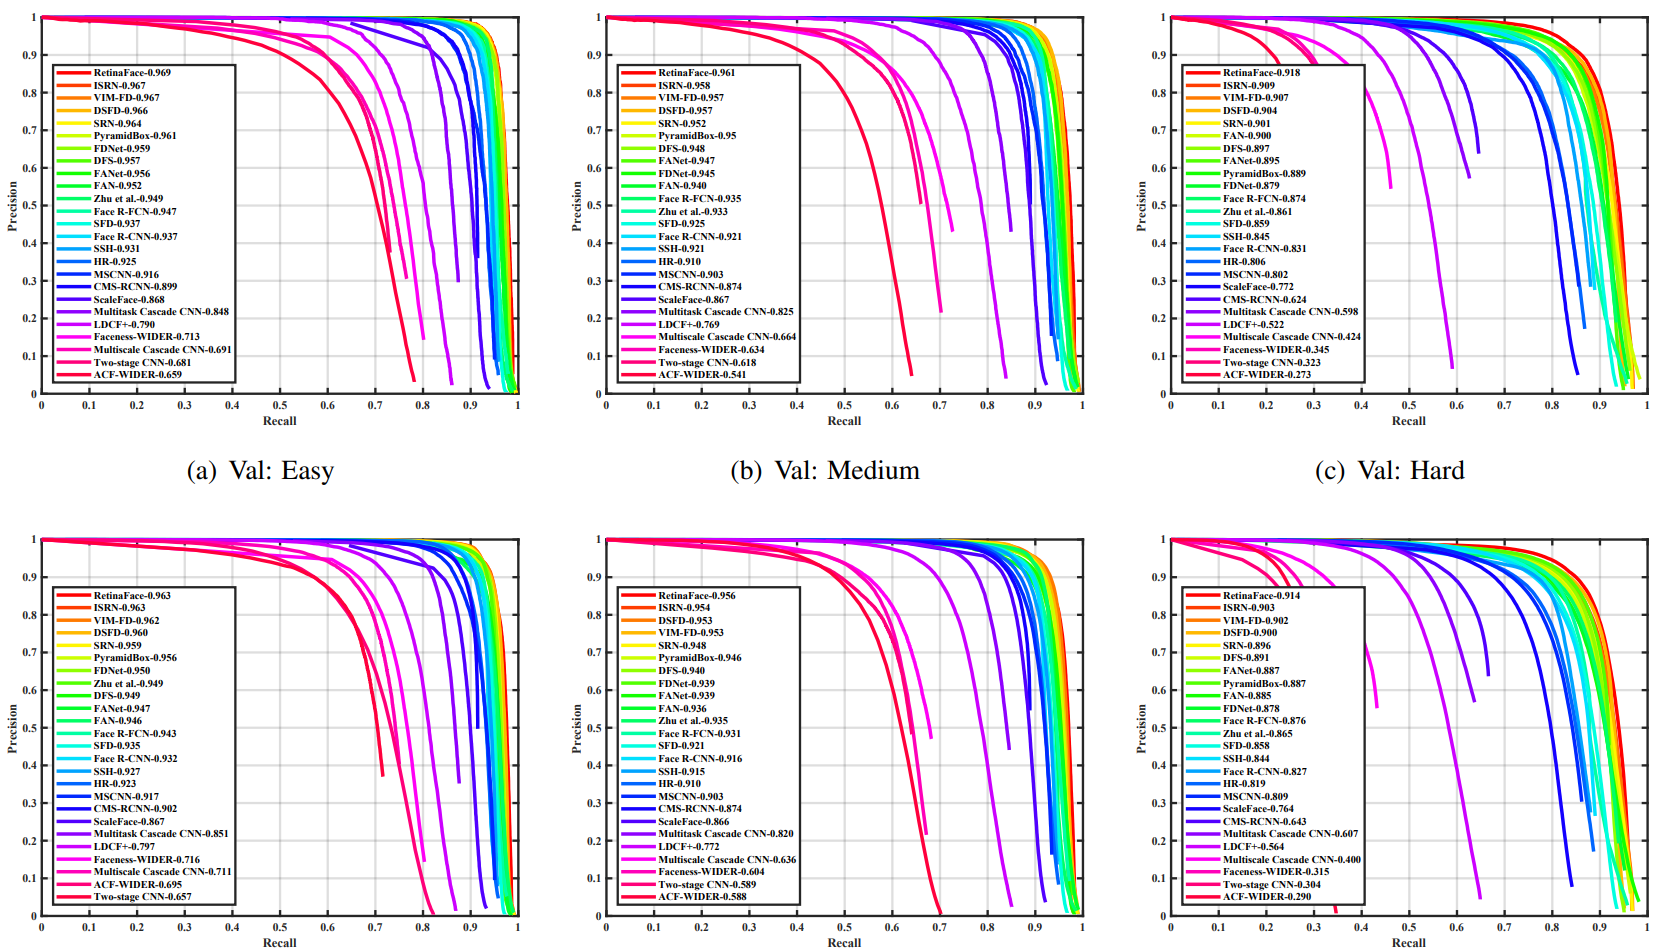
\includegraphics[width=\textwidth,height=0.50\textheight,keepaspectratio]{figures/images/chapter-11/retinaface/precision–recall-for-test-and-val-set.png}
\caption{Precision--recall curves for RetinaFace compared with other face detection methods on the WIDER FACE validation set, divided into easy, medium, and hard subsets \cite{deng2020retinaface}. Backbone-specific results for the PyTorch implementation are reported separately in Table~\ref{tab:retinaface_widerface}.}
\label{fig:retinaface_widerface_combined}
\end{figure}

In addition to WIDER FACE, the implementation also reports results on the FDDB benchmark, as shown in Table~\ref{tab:retinaface_fddb}. Both backbones achieve high performance, with \texttt{MobileNet0.25} reaching 98.64\% and \texttt{ResNet50} achieving 99.22\%.

\begin{table}[H]
\centering
\caption{Reported FDDB performance of the RetinaFace PyTorch implementation \cite{biubug6_retinaface}.}
\label{tab:retinaface_fddb}
\begin{tabular}{lc}
\toprule
Backbone & Performance \\
\midrule
MobileNet0.25 & 98.64\% \\
ResNet50 & 99.22\% \\
\bottomrule
\end{tabular}
\end{table}

The FDDB evaluation curves (Figure~\ref{fig:retinaface_fddb}) further indicate high true positive rates across a wide range of \gls{false positive} counts. This behavior was consistent with observations from the implemented system, where the model rarely produced false detections and maintained reliable localization.

\begin{figure}[H]
\centering
\makebox[\textwidth][c]{
    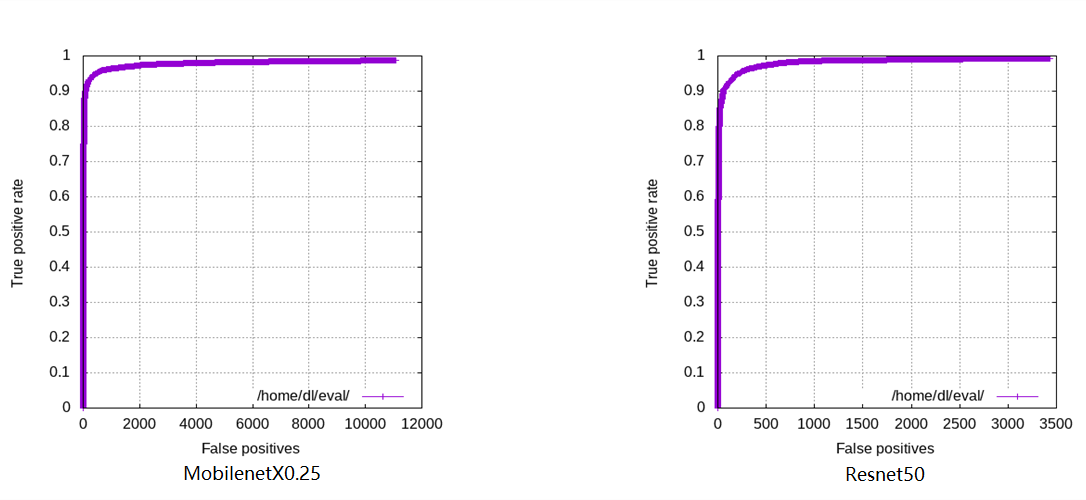
\includegraphics[width=1.2\textwidth]{figures/images/chapter-11/retinaface/fddb_curves.png}
}
\caption{FDDB evaluation curves reported for the RetinaFace implementation using the MobileNet0.25 and ResNet50 backbones \cite{biubug6_retinaface}.}
\label{fig:retinaface_fddb}
\end{figure}

The face detection component demonstrated reliable and consistent performance within the \gls{anonymization} pipeline. While minor performance degradation was observed for small or heavily occluded faces, the model provided sufficiently accurate detections for downstream \gls{anonymization}. This confirms that the pre-trained RetinaFace model is well-suited for real-time face detection in the proposed system.


\methodheading{Text Detection and Recognition}

Text detection and recognition were performed using pre-trained PaddleOCR models integrated into the \gls{anonymization} pipeline \cite{paddleocr_overview}. The system used the \texttt{PP-OCRv5\_mobile\_det} model for text detection and the \texttt{en\_PP-OCRv5\_mobile\_rec} model for text recognition, both executed on CPU. Table~\ref{tab:paddleocr_text_models} summarizes the reported benchmark results for the selected models. The detection model achieves an Hmean of 79.0, while the recognition model reports an average accuracy of 85.25. These values provide a reference for the observed system performance.

\begin{table}[!htbp]
\centering
\begin{tabular}{lcccc}
\toprule
Model & Task & Metric & CPU Time (ms) & Size (MB) \\
\midrule
PP-OCRv5\_mobile\_det & Detection & Hmean = 79.0 & 51.00 / 28.58 & 4.7 \\
en\_PP-OCRv5\_mobile\_rec & Recognition & Avg Accuracy = 85.25 & -- & 7.5 \\
\bottomrule
\end{tabular}
\caption{Official PaddleOCR benchmark results for the text detection and recognition models used in the system \cite{paddleocr_model_list_2x}.}
\label{tab:paddleocr_text_models}
\end{table}

In the implemented system, PaddleOCR produced accurate and consistent text localization across both document-like and natural scene images. The detection model generated tight \gls{bounding box}es around text regions, while the recognition model correctly transcribed most detected text, including multi-line and structured content.

Unlike the RetinaFace evaluation, detailed precision--recall curves were not available for the selected PaddleOCR configuration. The official documentation instead provides aggregate benchmark metrics, which limits direct comparison of detection behavior across varying thresholds. As a result, qualitative system-level examples are included to illustrate performance in practical scenarios. Figure~\ref{fig:text_detection_recognition_examples} presents examples of text detection and recognition results. In the document-like example, the model demonstrates high accuracy in detecting structured text, with precise localization and correct recognition of multiple lines. In the scene example, the model successfully identifies text under more challenging conditions, including varying backgrounds, perspective distortion, and uneven lighting.

\begin{figure}[H]
    \centering

    \begin{minipage}{\textwidth}
        \centering
        
\includegraphics[width=1.0\textwidth]{figures/images/chapter-11/text-detection/IMG_7358_ocr_comparison.png}
        \par\vspace{2pt} \small (a) Example from a document-like image (Photo by author. Source: \textit{A Brief History of Time} \cite{hawking2017}).
    \end{minipage}

    \vspace{0.0cm}

    \begin{minipage}{\textwidth}
        \centering
        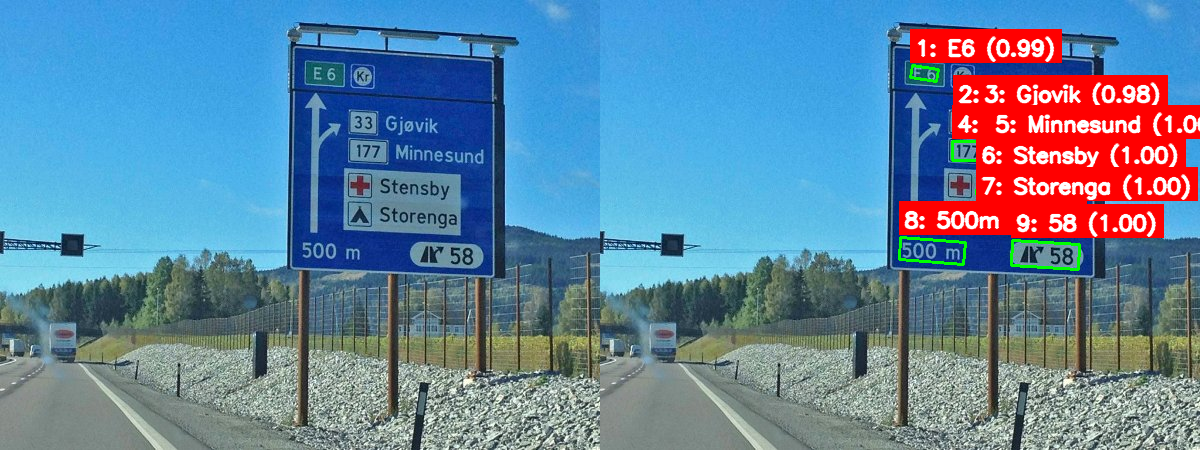
\includegraphics[width=1.0\textwidth]{figures/images/chapter-11/text-detection/gjovik_ocr_comparison.png}
        \par\vspace{2pt} \small (b) Example from a scene image (Image source: \cite{smaalenene2014}).
    \end{minipage}

    \caption{Representative text detection and recognition results produced by PaddleOCR in the integrated \gls{anonymization} pipeline.}
    \label{fig:text_detection_recognition_examples}
\end{figure}

While the overall performance was strong, some limitations were observed. Recognition accuracy decreased for small, low-resolution, or low-contrast text, particularly in complex scene images. Minor errors such as incorrect characters or missed spaces were occasionally present, although these did not significantly impact the \gls{anonymization} process. Despite these limitations, the models maintained stable performance across diverse input conditions and operated efficiently on CPU (Section~\ref{sec:performance_tests}), enabling responsive \gls{inference} within the pipeline. The PaddleOCR-based component provided sufficiently accurate text localization and recognition for reliable \gls{anonymization} in the proposed system.


\methodheading{General Object Detection}

General \gls{object detection} was performed using a pre-trained \gls{yolox-s} model integrated into the \gls{anonymization} pipeline \cite{yolox}. The same model architecture was also used for the custom-trained barcode and license plate detectors, resulting in consistent detection behavior across components.

To make the general object detector more suitable for \gls{SafeVision}, the original COCO output classes were reduced to a smaller set of privacy-relevant categories which contains 80 object classes. In this project, these classes are mapped to a smaller set of application-specific categories, including \texttt{PERSON}, \texttt{VEHICLE}, \texttt{ANIMAL}, \texttt{BAG}, \texttt{ELECTRONIC}, and \texttt{STREET\_OBJECT}. This mapping simplifies the detection output and allows the system allows the system to prioritize entities for \gls{anonymization}. Classes not relevant for the application are filtered out during postprocessing.

\gls{yolox} is a one-stage object detector designed for efficient and real-time \gls{inference} \cite{yolox}. The \gls{yolox-s} variant used in this project provides a good balance between detection accuracy and computational efficiency, making it suitable for deployment in practical applications. Reported benchmark results on the COCO dataset show that \gls{yolox} achieves competitive performance compared to other real-time detectors \cite{yolox}. As shown in Table~\ref{tab:yolox_benchmark}, the \gls{yolox-s} model achieves approximately 40.5 AP while maintaining real-time \gls{inference} speed.

\begin{table}[H]
\centering
\begin{tabular}{lcc}
\toprule
Model & AP (COCO) & Frames Per Second (\acrshort{fps}) \\
\midrule
\gls{yolox-s} & $\sim$40.5 & $\sim$60+ \acrshort{fps} \\
\bottomrule
\end{tabular}
\caption{Reported \gls{yolox} performance on the COCO dataset (\gls{yolox-s} variant) \cite{yolox}.}
\label{tab:yolox_benchmark}
\end{table}

Figure~\ref{fig:yolox_benchmark_tradeoff} illustrates the relationship between model complexity and detection performance for \gls{yolox} and comparable models. The \gls{yolox-s} variant achieves a strong balance between accuracy and efficiency, outperforming several lightweight alternatives while maintaining a relatively low number of parameters.

\begin{figure}[H]
\centering
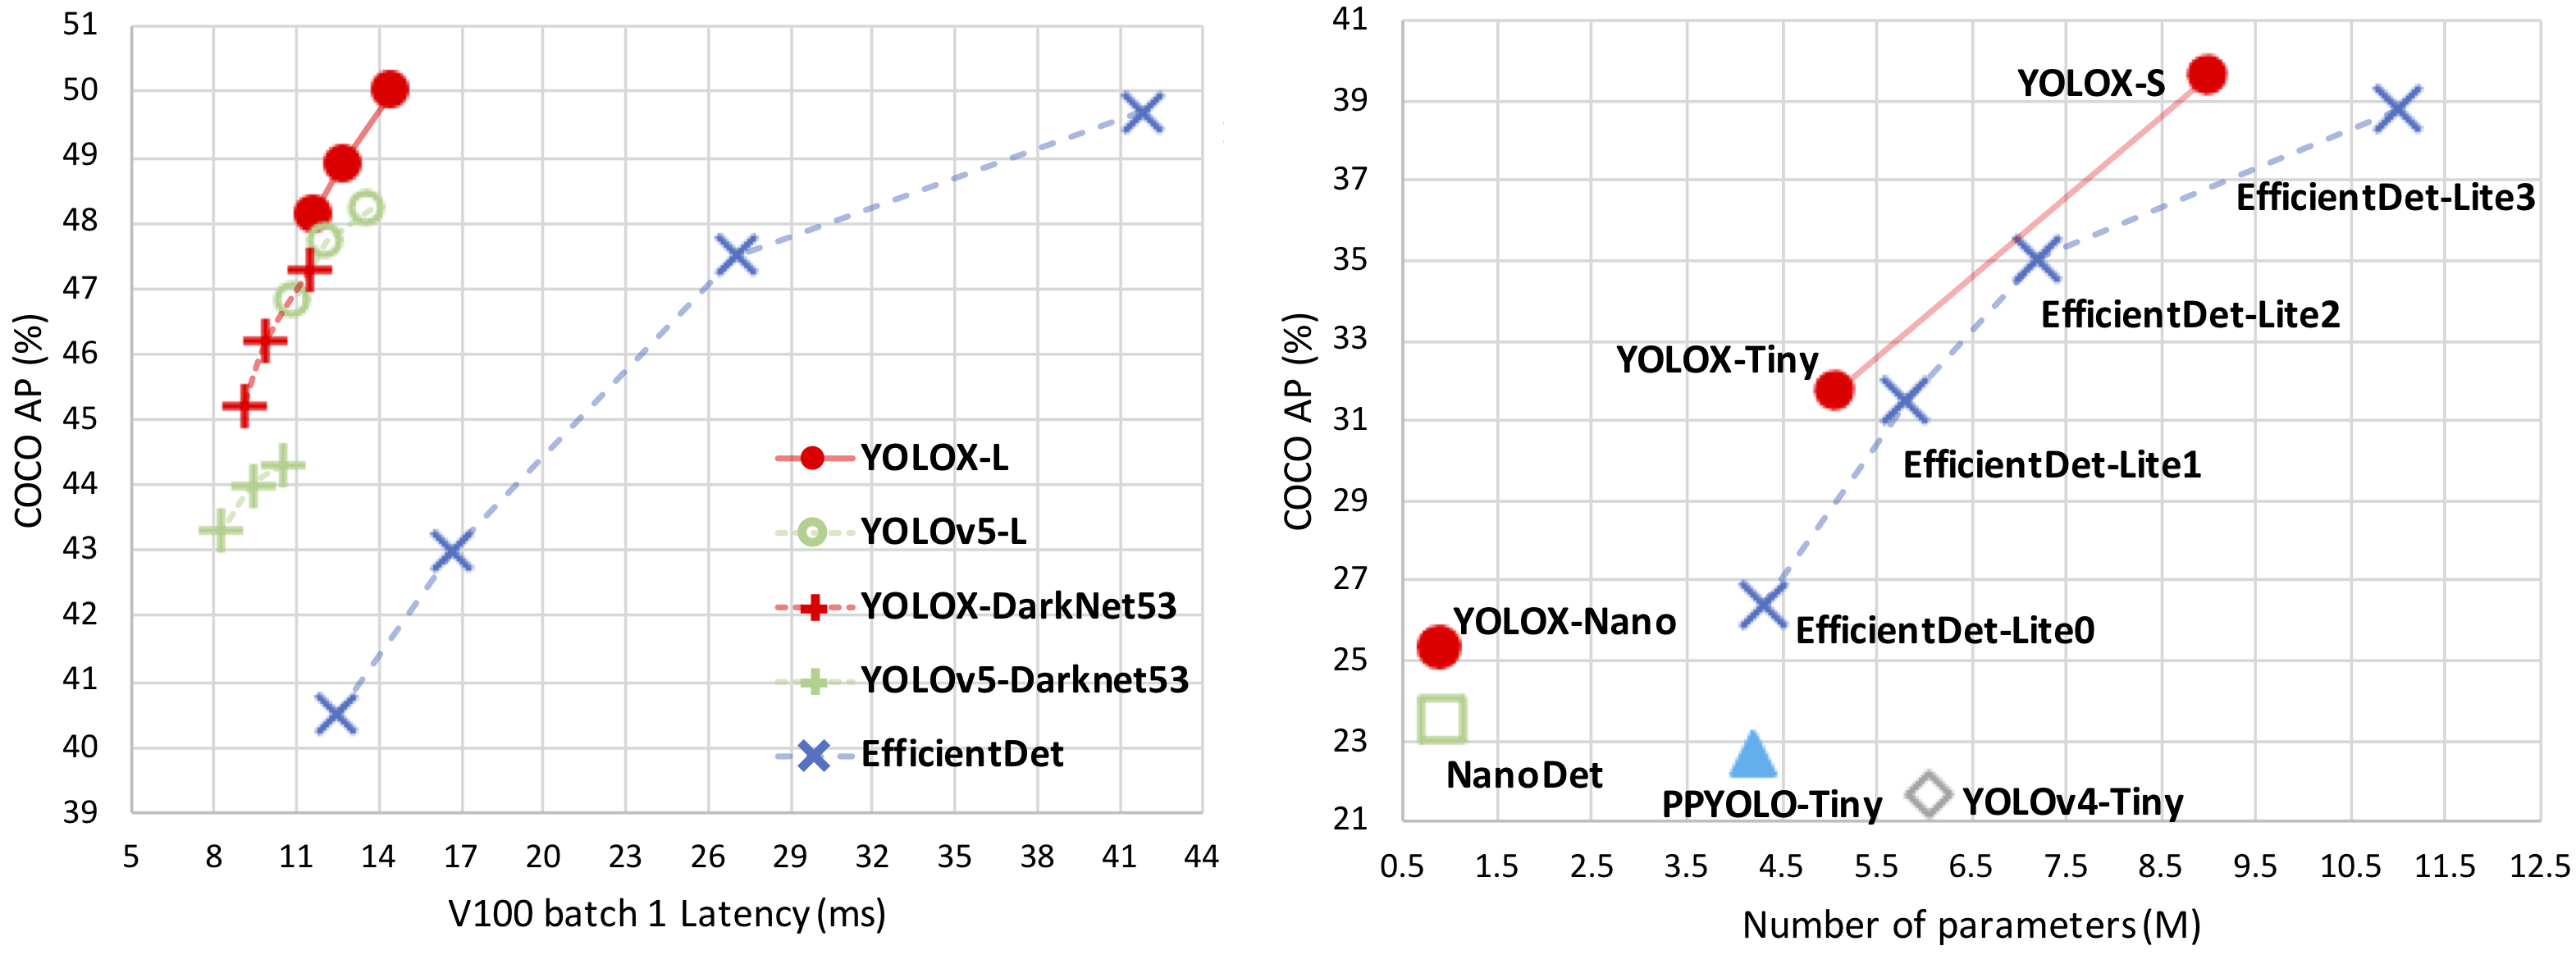
\includegraphics[width=1.1\textwidth]{figures/images/chapter-11/yolox/yolox_tradeoff.png}
\caption{Comparison of \gls{object detection} models showing the relationship between number of parameters and COCO AP. \gls{yolox-s} achieves a favorable balance between accuracy and model complexity \cite{yolox}.}
\label{fig:yolox_benchmark_tradeoff}
\end{figure}

Figure~\ref{fig:yolox_detection_example} shows an example of \gls{object detection} using the \gls{yolox} model in the implemented system. The model successfully detects multiple object types in the scene and assigns them to the corresponding application-specific categories.

\begin{figure}[H]
\centering
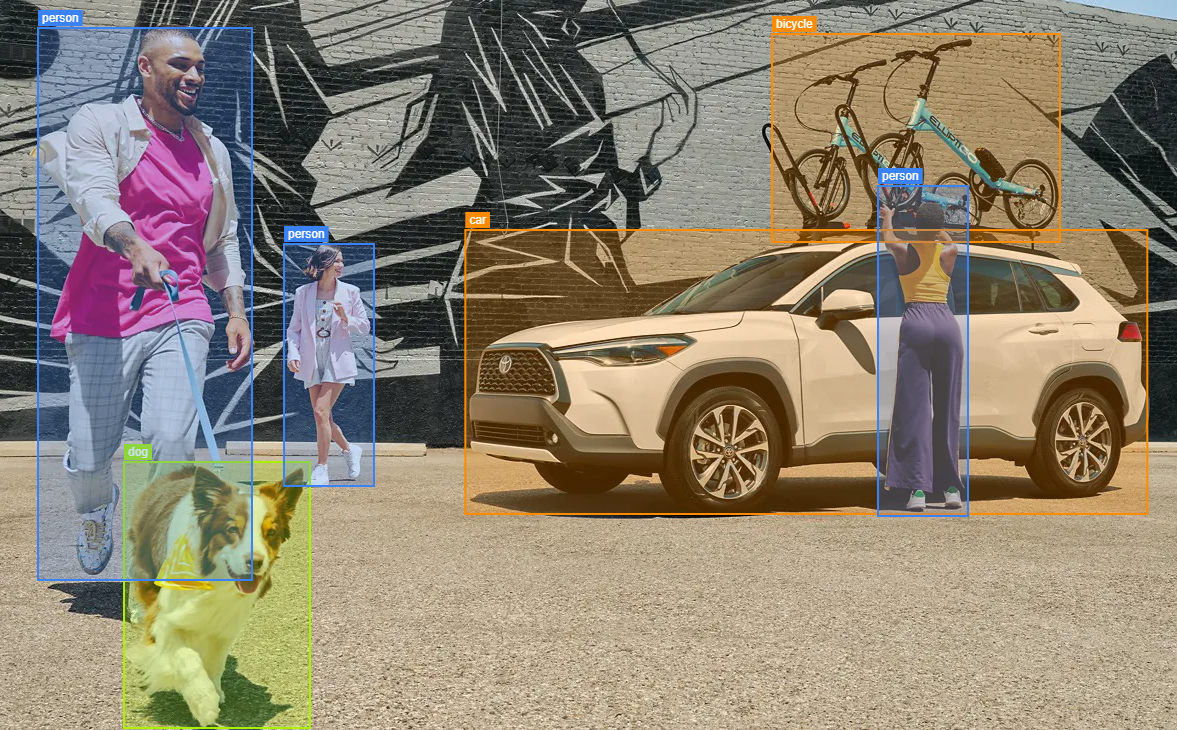
\includegraphics[width=1.1\textwidth]{figures/images/chapter-11/yolox/example.png}
\caption{Example of \gls{object detection} using YOLOX. The figure shows detected objects and their corresponding categories used in the \gls{anonymization} pipeline (Image source: \cite{foxdealer2024}).}
\label{fig:yolox_detection_example}
\end{figure}

YOLOX-based \gls{object detection} component provides reliable detection of general objects and complements the custom-trained models by covering a broader set of categories. This improves the robustness of the \gls{anonymization} system in real-world scenarios.

\methodheading{Image \Gls{segmentation}}

Image \gls{segmentation} was performed using the pre-trained \gls{mobilesam} model integrated into the \gls{anonymization} pipeline. Unlike \gls{object detection} models that produce \gls{bounding box}es, \gls{mobilesam} generates pixel-level \gls{segmentation} masks, enabling more precise \gls{anonymization} of detected objects.

In the implemented system, \gls{segmentation} was applied only within detected \gls{bounding box}es. This reduced unnecessary computation and ensured that \gls{segmentation} was limited to relevant regions, improving both efficiency and output quality. Figure~\ref{fig:segmentation_comparison} shows a comparison between \gls{bounding box} based \gls{anonymization} and \gls{segmentation} based \gls{anonymization}. The results demonstrate that \gls{mobilesam} produces masks that closely follow object boundaries, significantly reducing the inclusion of background regions. This was beneficial for irregularly shaped objects, where \gls{bounding box}es often covered large amounts of irrelevant area.

\begin{figure}[H]
\centering
\begin{subfigure}{0.32\textwidth}
\centering
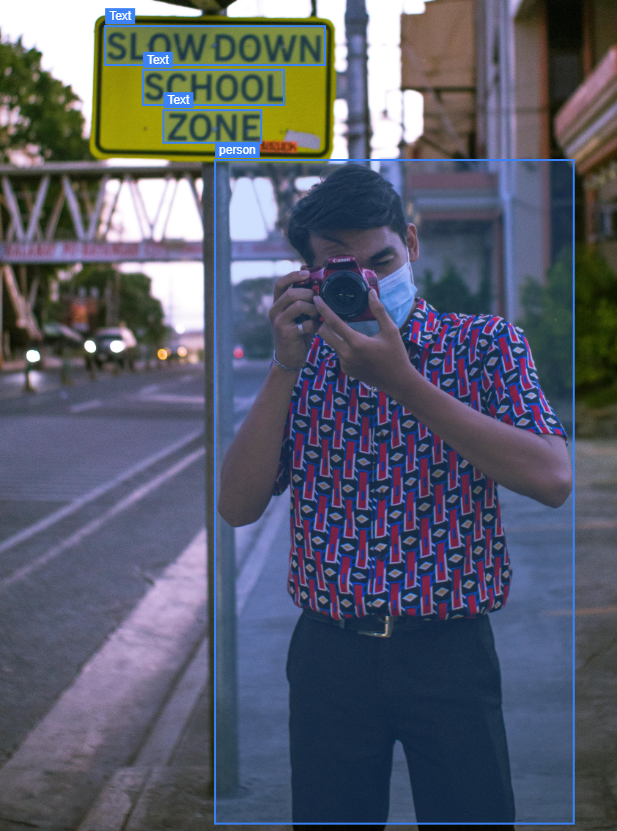
\includegraphics[width=\linewidth]{figures/images/chapter-11/segmentation/detection.png}
\caption{Detections filtered}
\end{subfigure}
\hfill
\begin{subfigure}{0.32\textwidth}
\centering

\includegraphics[width=\linewidth]{figures/images/chapter-11/segmentation/redaction-box.png}
\caption{Without \gls{segmentation}}
\end{subfigure}
\hfill
\begin{subfigure}{0.32\textwidth}
\centering
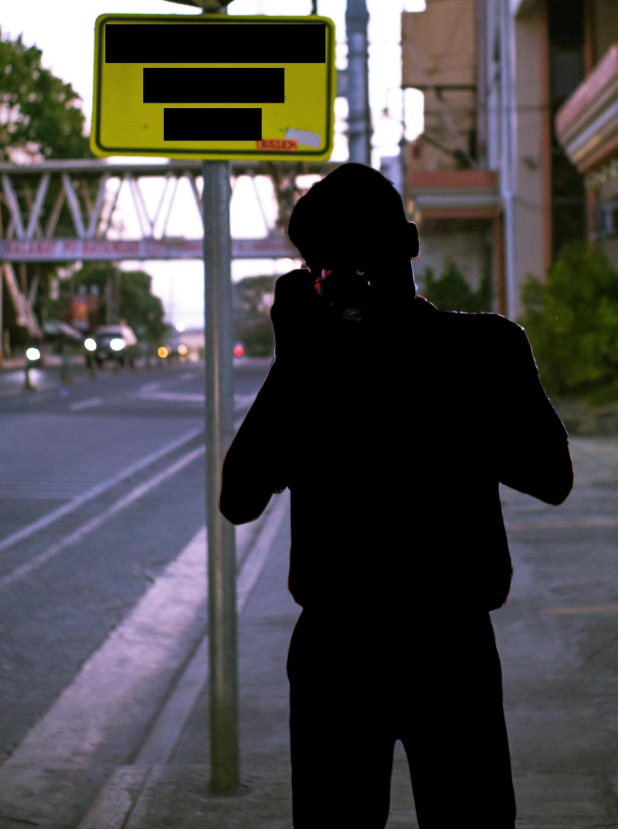
\includegraphics[width=\linewidth]{figures/images/chapter-11/segmentation/redaction-segmented.png}
\caption{With \gls{segmentation}}
\end{subfigure}
\caption{Comparison of \gls{anonymization} with and without \gls{segmentation}. (a) Detected region, (b) \gls{bounding box} based \gls{anonymization}, and (c) \gls{segmentation} based \gls{anonymization} using \gls{mobilesam}. Text regions are not segmented. (Image source from \cite{pavel2021})}
\label{fig:segmentation_comparison}
\end{figure}

In practice, \gls{mobilesam} produced stable and high-quality \gls{segmentation} masks across a range of object types. The masks were generally well-aligned with object boundaries, leading to more visually precise \gls{anonymization} compared to \gls{bounding box} based approaches. However, some limitations were observed. \Gls{segmentation} quality decreased for very small or low-resolution objects, and slight boundary inaccuracies were occasionally present in complex scenes with overlapping objects or weak contrast. Despite this, the \gls{segmentation} output remained sufficiently accurate for the intended \gls{anonymization} task.

Table~\ref{tab:mobilesam_comparison} summarizes benchmark results reported for \gls{mobilesam}. Compared to the original \acrshort{sam}, \gls{mobilesam} is significantly more efficient while maintaining similar \gls{segmentation} performance. These results are consistent with observations from the implemented system, where \gls{segmentation} added only a small computational overhead and remained suitable for near real-time processing. This made it well-suited for integration into the real-time \gls{anonymization} pipeline

\begin{table}[H]
\centering
\begin{tabular}{lcc}
\toprule
Metric & SAM & MobileSAM \\
\midrule
Model size & $\sim$632M params & $\sim$5.8M params \\
Speed & Baseline & 5--38$\times$ faster \\
\Gls{inference} time & $\sim$50--100 ms & $\sim$10 ms \\
m\acrshort{iou} & $\sim$0.76--0.78 & $\sim$0.74 \\
\bottomrule
\end{tabular}
\caption{Comparison between \acrshort{sam} and \gls{mobilesam} based on reported benchmark results \cite{mobilesam}.}
\label{tab:mobilesam_comparison}
\end{table}

%------------------------11.2-------------------------

\section{Custom-Trained Detection Models}
\label{sec:custom_trained_detection_models}

Two custom \gls{object detection} models were developed in this project: one for barcode detection and one for license plate detection. This section presents the final test-set results and the final models selected for use in the proposed system. Detailed training configurations, training curves, precision--recall curves, and confusion matrices are provided in Appendix~\ref{app:custom_model_evaluation}.

\methodheading{Barcode Detection Results}

\begin{figure}[H]
\centering
\begin{subfigure}{0.40\textwidth}
\centering
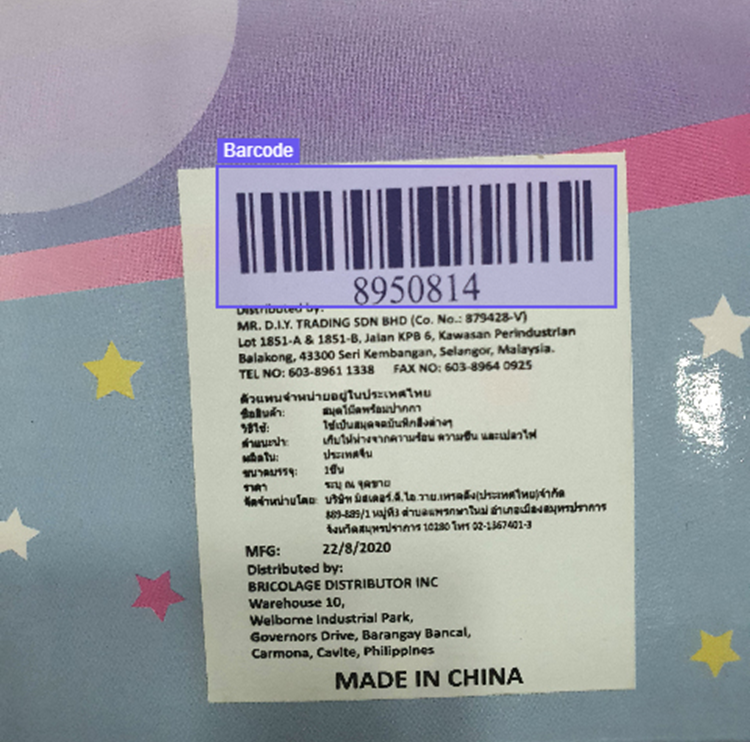
\includegraphics[width=\linewidth]{figures/images/chapter-11/qr-bar/example01.png}
\end{subfigure}
\hfill
\begin{subfigure}{0.40\textwidth}
\centering
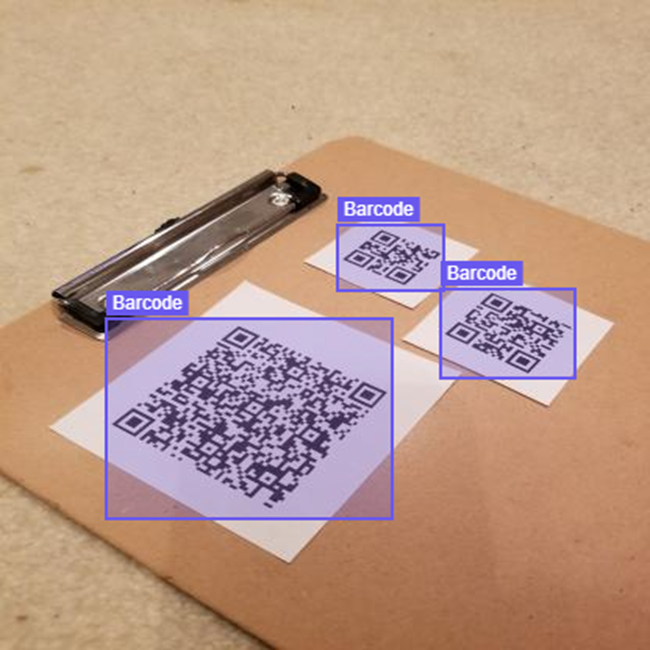
\includegraphics[width=\linewidth]{figures/images/chapter-11/qr-bar/example02.png}
\end{subfigure}
\caption{Examples of barcode and QR-code detection. Images from the test set, sources \cite{benchmark_barcode_kaggle,barcode_qr_kaggle}.}
\label{fig:qr_bar_examples}
\end{figure}

The final barcode detection model was evaluated on an unseen test set. Since the model achieved strong performance across all evaluation metrics, no further barcode model iterations were considered necessary.

\begin{table}[H]
\centering
\caption{Final barcode detection performance at confidence threshold $0.3$.}
\begin{tabular}{lcccccc}
\toprule
Model & TP & FP & FN & Precision & Recall & F1 Score \\
\midrule
Final barcode model & 1699 & 53 & 7 & 96.97\% & 99.59\% & 0.983 \\
\bottomrule
\end{tabular}
\label{tab:barcode_results}
\end{table}

As shown in Table~\ref{tab:barcode_results}, the barcode model achieved high precision and recall. The model missed 7 barcodes on the test set, indicating that it is reliable for detecting barcode and QR-code objects in the proposed system.

\methodheading{License Plate Detection Results}

\begin{figure}[H]
\centering
\begin{subfigure}{0.48\textwidth}
\centering
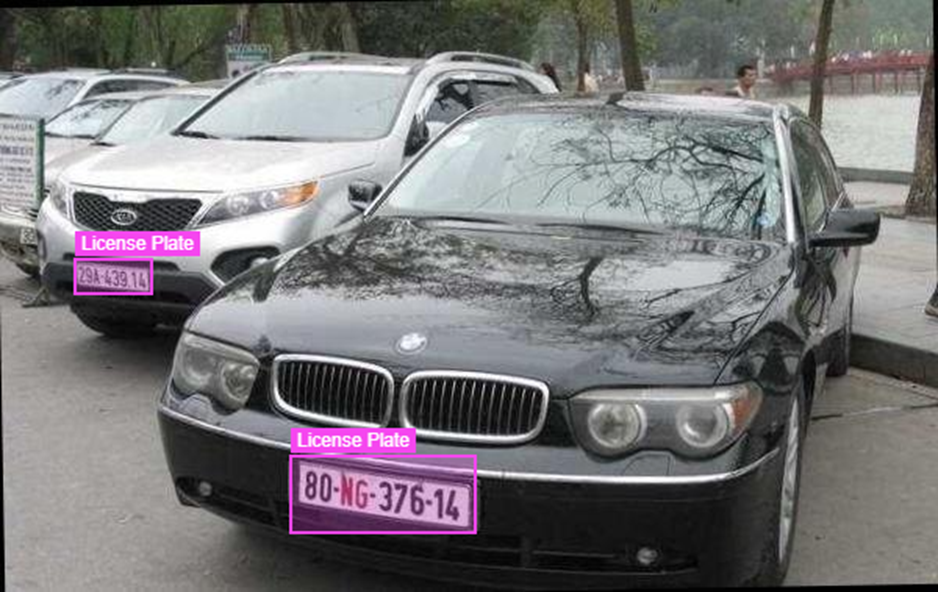
\includegraphics[width=\linewidth]{figures/images/chapter-11/licenseplate/example01.png}
\end{subfigure}
\hfill
\begin{subfigure}{0.48\textwidth}
\centering
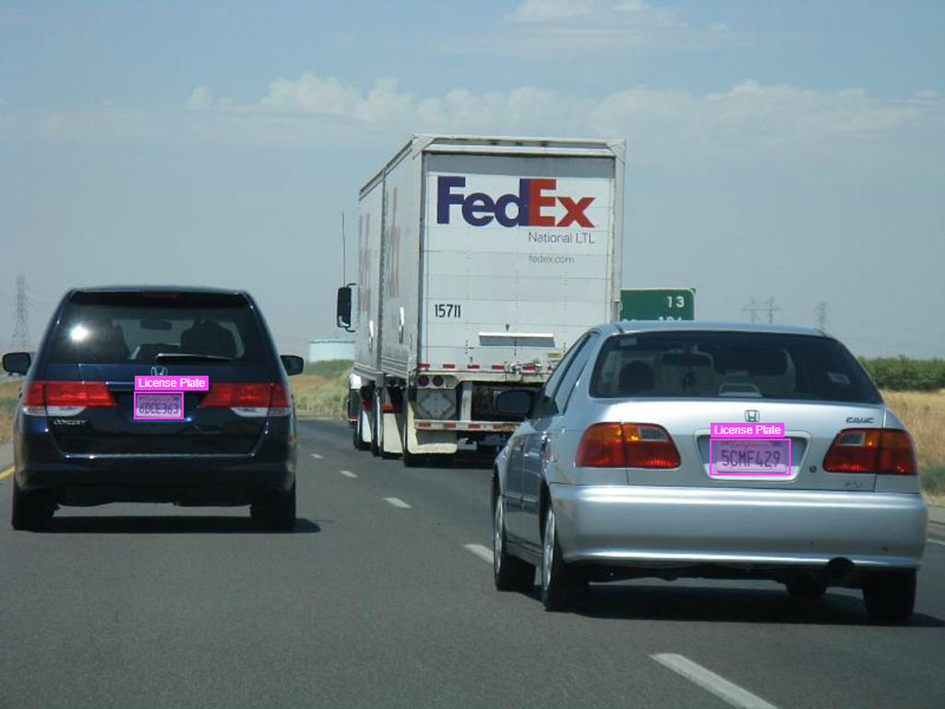
\includegraphics[width=\linewidth]{figures/images/chapter-11/licenseplate/example02.png}
\end{subfigure}
\caption{Examples of license plate detection. Images from the test set, sources \cite{lp_dataset_1,lp_dataset_2}.}
\label{fig:licenseplate_examples}
\end{figure}

For license plate detection, two configurations were evaluated to investigate the effect of increased input resolution on detection performance. Model v1 achieved slightly higher precision, while model v0 achieved higher recall and a higher F1-score.

\begin{table}[H]
\centering
\caption{License plate detection performance at confidence threshold $0.3$.}
\begin{tabular}{lccccccc}
\toprule
Model & Input Size & TP & FP & FN & Precision & Recall & F1 Score \\
\midrule
v0 & $640\times640$ & 1946 & 98 & 111 & 95.21\% & 94.60\% & \textbf{0.949} \\
v1 & $960\times960$ & 1964 & 80 & 186 & \textbf{96.09\%} & 91.35\% & 0.937 \\
\bottomrule
\end{tabular}
\label{tab:license_plate_results}
\end{table}

As shown in Table~\ref{tab:license_plate_results}, v1 produced fewer \gls{false positive}s and therefore achieved slightly higher precision. However, v0 missed fewer license plates and achieved the highest recall and F1-score. Since the proposed system benefits from detecting as many license plates as possible while still maintaining high precision, the v0 configuration was selected as the final license plate detection model. Further details for both license plate models are provided in
Appendix~\ref{app:license_plate_results}.

\methodheading{Named Entity Recognition Results}

\label{sec:ner_results}
The final NER model was evaluated on a held-out test split constructed from the merged training pipeline. The model achieved high aggregate scores on this test split.

\begin{table}[H]
\centering
\caption{Final NER model performance on the constructed held-out test split.}
\begin{tabular}{lcccc}
\toprule
Model & Loss & Precision & Recall & F1 Score \\
\midrule
Final NER model & 0.0061 & 99.73\% & 99.78\% & 0.9975 \\
\bottomrule
\end{tabular}
\label{tab:ner_results_main}
\end{table}

Although the NER model achieved near-perfect results on the constructed held-out test split, these results were not considered fully representative of practical system performance. Since the test split was derived from the same synthetic and
converted-data pipeline used during training, it remained relatively close to the training distribution.

\begin{table}[H]
\centering
\caption{Overall NER performance on the harder \acrshort{ocr} oriented test set.}
\begin{tabular}{lccc}
\toprule
Evaluation set & Precision & Recall & F1 Score \\
\midrule
Hard test set & 91.32\% & 96.13\% & 0.9366 \\
\bottomrule
\end{tabular}
\label{tab:ner_results_hard}
\end{table}

Additional evaluation on a separate harder \acrshort{ocr} oriented test set was performed. As shown in Table~\ref{tab:ner_results_hard}, the NER model achieved lower performance on the harder \acrshort{ocr} oriented test set than on the constructed held out split. This indicates that the near perfect results on the merged test split overestimated the model’s practical robustness, particularly in noisier and more semantically ambiguous \acrshort{ocr} scenarios.


\begin{figure}[H]
\centering
\begin{subfigure}{0.60\textwidth}
\centering
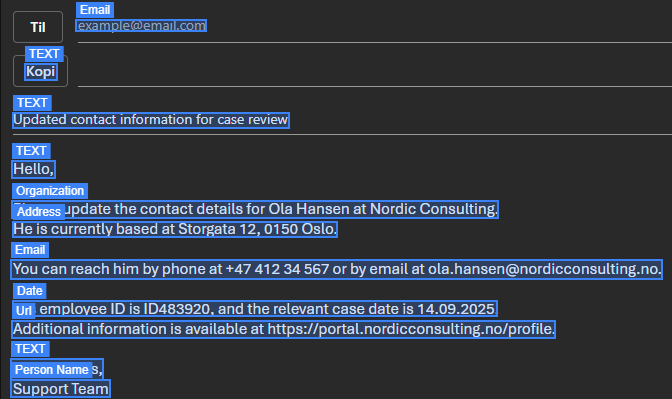
\includegraphics[width=\linewidth]{figures/images/chapter-11/ner/email.png}
\caption{Self-produced illustrative email example.}
\end{subfigure}
\hfill
\begin{subfigure}{0.60\textwidth}
\centering

\includegraphics[width=\linewidth]{figures/images/chapter-11/ner/student-id.png}
\caption{Real-world student ID example.}
\end{subfigure}
\caption{Examples of \acrshort{ocr} based text categorization. Photos by the authors.}
\label{fig:ner_real_vs_controlled}
\end{figure}

Even though the evaluation on the constructed test split shows a high score, Figure~\ref{fig:ner_real_vs_controlled} indicates that the NER-based text categorization is not yet well suited for real-life document scenarios. While the controlled example shows that the model can assign relevant categories in a
structured setting, the real-world document example shows that it still has difficulty separating different entity categories reliably.

These limitations meant that the NER model was not used as a standalone text categorization component in the final system. Instead, the final text-analysis pipeline used a hybrid approach that combined NER predictions with contextual rules and post-processing filters in order to achieve more stable categorization of \acrshort{ocr} extracted text. Training details and further evaluation results are provided in Appendix~\ref{app:ner_evaluation}.

\section{Video Processing Results}
\label{sec:video_processing_results}

Video processing was evaluated as a system-level extension of the image detection and redaction pipeline. The evaluation examined whether the implemented video pipeline could detect, propagate, track, and redact sensitive regions across complete video sequences. This section presents the main results, while Appendix~\ref{app:video_evaluation_details} provides the detailed evaluation setup, annotation procedure, metrics, and additional temporal coverage analysis.

\methodheading{Qualitative Results}

Across the tested videos, the pipeline was able to maintain sensitive-region detections across complete video sequences and apply redaction based on the generated frame-wise manifest. This manifest allowed \gls{bounding box}es to be displayed across frames and enabled the video workflow to reuse the same inspection step as the image workflow. Figure~\ref{fig:video_redaction_example} shows an example where detected regions are segmented and pixelated in the final video output.

\begin{figure}[H]
\centering
\begin{subfigure}{0.48\textwidth}
\centering
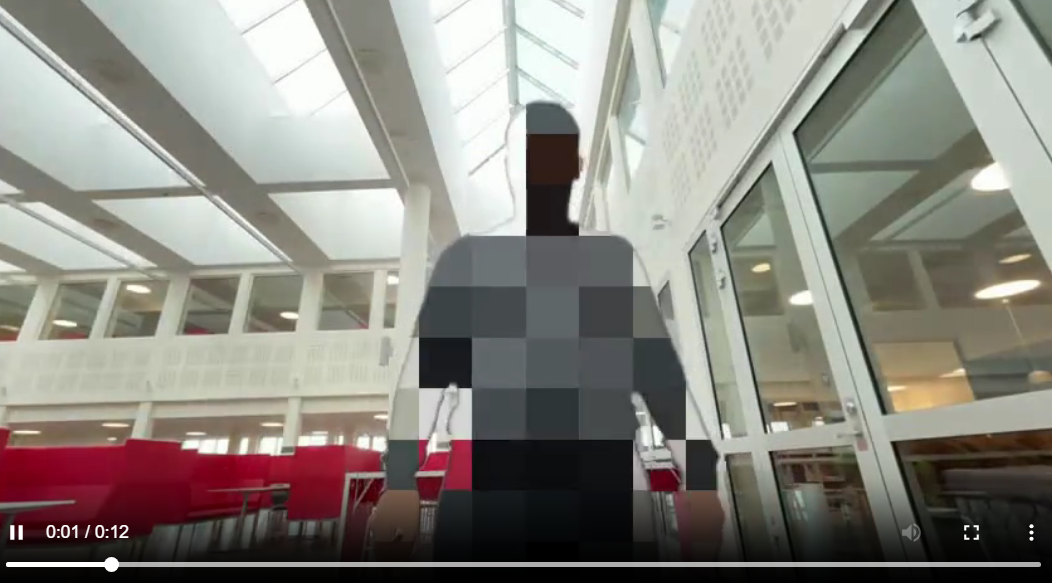
\includegraphics[width=\linewidth]{figures/images/chapter-11/segmentation pixelate video2.png}
\end{subfigure}
\hfill
\begin{subfigure}{0.48\textwidth}
\centering
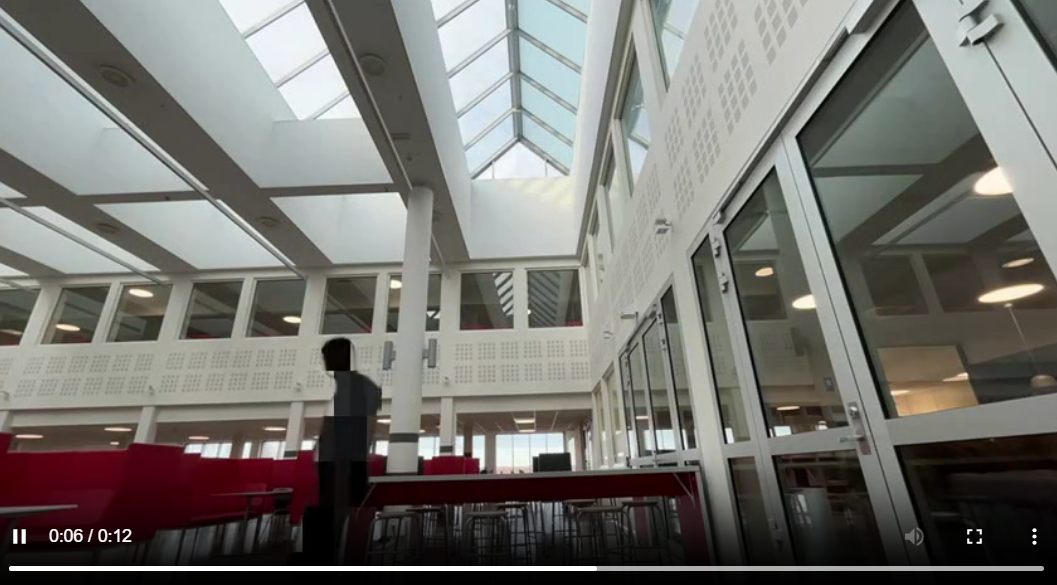
\includegraphics[width=\linewidth]{figures/images/chapter-11/segmentation pixelate video.png}
\end{subfigure}
\caption{Example of video redaction. The redaction stage uses the frame-wise manifest to apply \gls{segmentation} and pixelation to regions in the video. Video by authors.}
\label{fig:video_redaction_example}
\end{figure}

\methodheading{Automatic Kalman-Based Prediction Results}

Kalman-based prediction preserved accurate \gls{bounding box}es between detection frames, particularly when detector updates were performed frequently. Because full detection is only executed on selected frames, the most important evaluation cases were the non-detection frames, where object positions had to be estimated without new detector output.

\begin{table}[H]
\centering
\small
\setlength{\tabcolsep}{5pt}
\begin{tabular}{rcccc}
\toprule
\textbf{\texttt{detect\_every}} & \textbf{Boxes} & \textbf{Mean \acrshort{iou}} & \textbf{Mean coverage} & \textbf{$\geq$90\% coverage} \\
\midrule
2  & 819  & 0.963 & 0.982 & 98.7\% \\
5  & 1312 & 0.922 & 0.958 & 92.6\% \\
10 & 1475 & 0.851 & 0.920 & 80.1\% \\
\bottomrule
\end{tabular}

\caption{Kalman based prediction accuracy on non detection frames across the three evaluated videos. ``Boxes'' refers to human labeled boxes. Mean \acrshort{iou} measures bounding box alignment, while mean coverage measures how much of the human-labeled sensitive regions were covered by the predicted boxes.}
\label{tab:kalman_prediction_accuracy}
\end{table}

Frequent detector updates produced the strongest prediction results, as shown in Table~\ref{tab:kalman_prediction_accuracy}. With \texttt{detect\_every = 2}, the mean \acrshort{iou} reached 0.963 and the mean sensitive-region coverage reached 0.982, showing that the predicted boxes were both well aligned and able to cover nearly all labeled sensitive regions. With \texttt{detect\_every = 5}, the mean \acrshort{iou} decreased to 0.922, while mean coverage remained high at 0.958. This indicates that moderate detector skipping still preserved useful prediction accuracy for review and redaction.

A clearer degradation appeared with \texttt{detect\_every = 10}. In this configuration, mean \acrshort{iou} decreased to 0.851, and the share of boxes with at least 90\% coverage decreased to 80.1\%. Longer prediction intervals therefore increased localization drift, especially in difficult frames with fast motion, scale changes, or multiple nearby objects. Even so, the mean coverage remained 0.920, meaning that the predicted boxes still covered most sensitive regions despite less precise alignment. This distinction is important for \gls{SafeVision}, since anonymization depends not only on tight localization, but also on whether sensitive content is sufficiently covered.

\methodheading{Manual Tracking Results}

Manual tracking was evaluated separately from automatic Kalman-based prediction to assess whether a user-selected region could be propagated reliably across a video sequence. The evaluation used the \texttt{car\_video} sequence and compared tracked \gls{bounding box}es with manually labeled ground-truth boxes. This tested the manual tracking path described in Section~\ref{sec:video_imp}, where TrackerViT is used as the primary OpenCV tracker and \acrshort{csrt} is available as a fallback.

The qualitative examples in Figure~\ref{fig:manual_tracking_examples} illustrate both successful and unsuccessful tracking behaviour. The tracker followed the selected vehicle accurately during normal visibility and when the object appeared smaller in the frame, but also produced one \gls{false positive} after the vehicle had left the scene. The corresponding quantitative results are summarized in Table~\ref{tab:manual_tracking_results}.

\begin{figure}[H]
\centering

\begin{subfigure}{0.48\textwidth}
    \centering
    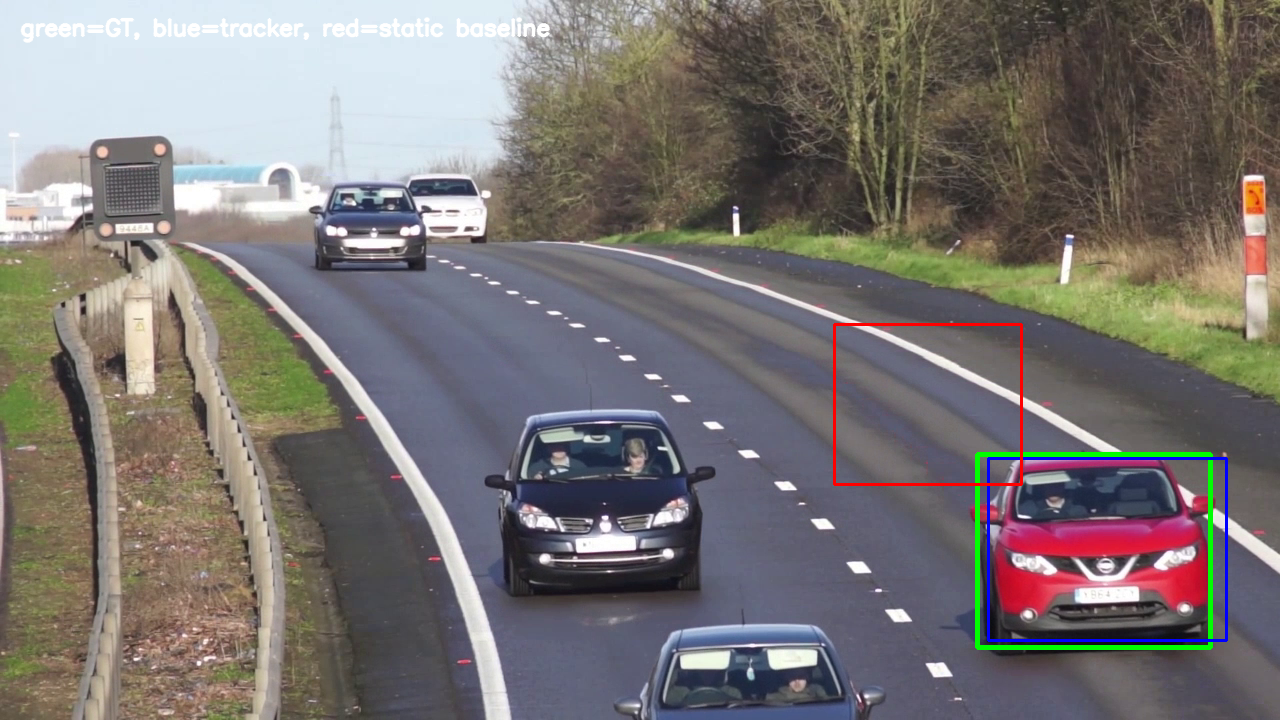
\includegraphics[width=\linewidth]{figures/images/chapter-11/car_track.png}
    \caption{Example of accurate manual tracking during normal object visibility.}
\end{subfigure}
\hfill
\begin{subfigure}{0.48\textwidth}
    \centering
    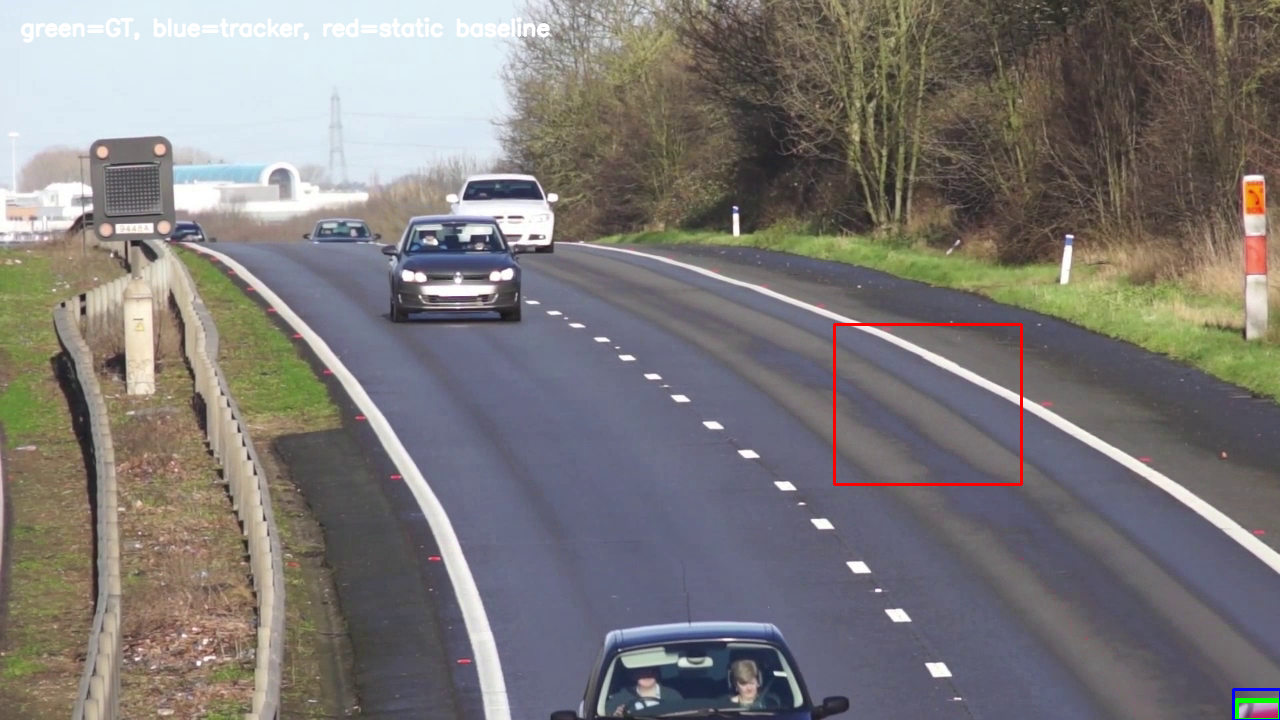
\includegraphics[width=\linewidth]{figures/images/chapter-11/false_car_track2.png}
    \caption{Example of accurate manual tracking during small object visibility.}
\end{subfigure}
\hfill
\begin{subfigure}{0.48\textwidth}
    \centering
    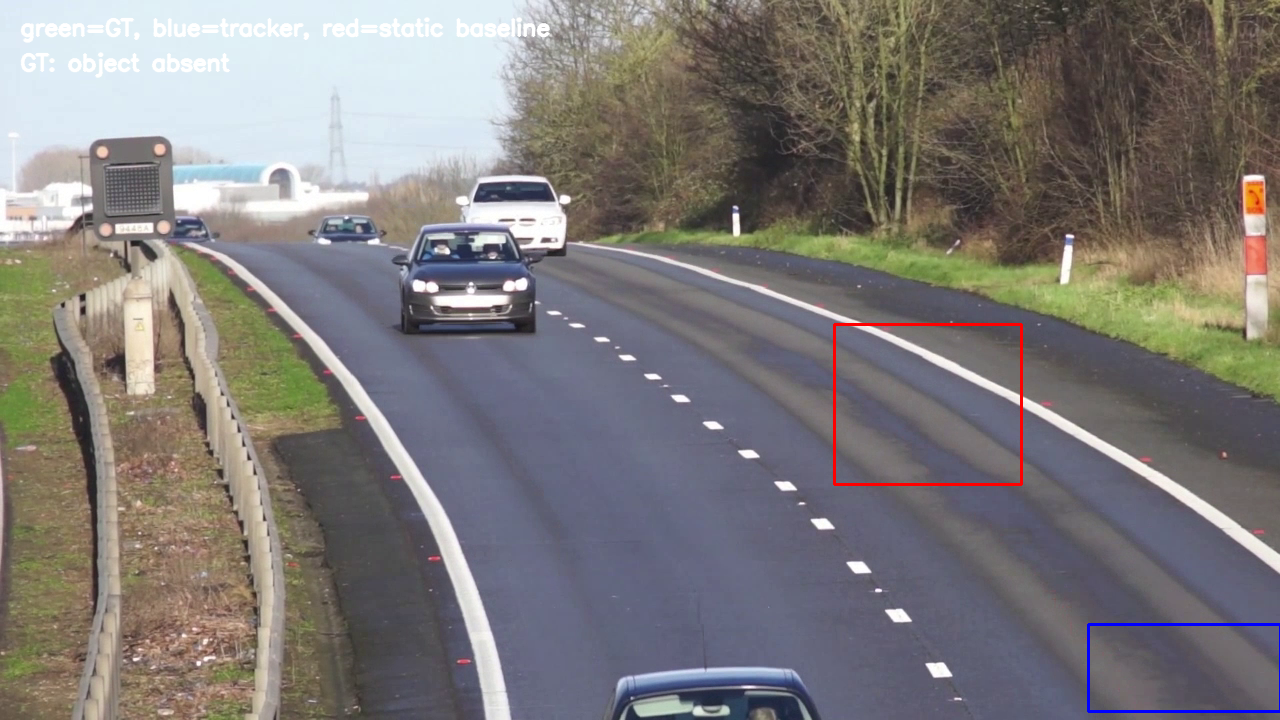
\includegraphics[width=\linewidth]{figures/images/chapter-11/false_car_track.png}
    \caption{Example of a \gls{false positive} after the object had left the scene.}
\end{subfigure}

\caption{Examples from the manual tracking evaluation. The red box shows the initial manually selected \gls{bounding box} used to start tracking, the green box shows the human-labeled ground truth, and the blue box shows the tracker output. Adapted from~\cite{pexels_highway_video}.}
\label{fig:manual_tracking_examples}
\end{figure}

\begin{table}[H]
\centering
\begin{tabular}{lc}
\toprule
\textbf{Metric} & \textbf{Result} \\
\midrule
Annotated frames & 25 \\
Visible annotated frames & 24 \\
Absent annotated frames & 1 \\
Mean \acrshort{iou} on visible frames & 0.8632 \\
Median \acrshort{iou} on visible frames & 0.8574 \\
Lowest \acrshort{iou} on visible frames & 0.6040 \\
Mean sensitive-region coverage & 0.9135 \\
Lowest sensitive-region coverage & 0.8188 \\
Missed visible frames & 0 \\
False positives on absent frames & 1 \\
Manual tracking runtime & 1.135 s \\
\bottomrule
\end{tabular}
\caption{Manual tracking results using human-labeled ground-truth boxes. Sensitive-region coverage measures how much of the human-labeled car region was covered by the tracked box.}
\label{tab:manual_tracking_results}
\end{table}

Across the visible frames, the manual tracker achieved a mean \acrshort{iou} of 0.8632 and a median \acrshort{iou} of 0.8574. The lowest visible-frame \acrshort{iou} was 0.6040, and the mean sensitive-region coverage was 0.9135, indicating that the tracked boxes generally remained well aligned with the annotated vehicle while also covering most of the sensitive region. No visible frames were missed, but one \gls{false positive} occurred after the vehicle had left the scene. These results show that manual tracking can support user-guided video redaction, but that user review remains important when an object leaves the frame, becomes occluded, or becomes difficult to distinguish from the background.

\methodheading{Processing Performance}

Processing performance was evaluated using different \texttt{detect\_every} values. This benchmark measured how detection frequency affected processing cost, while Table~\ref{tab:kalman_prediction_accuracy} shows the accuracy effect of the same configurations.

\begin{table}[H]
\centering
\begin{tabular}{rccc}
\toprule
\textbf{\texttt{detect\_every}} & \textbf{Detection calls} & \textbf{Processing time} & \textbf{Time reduction} \\
\midrule
1  & 261.00 & 231.71 s & -- \\
2  & 130.67 & 115.89 s & 50.0\% \\
5  & 52.33  & 46.61 s  & 79.9\% \\
10 & 26.33  & 23.57 s  & 89.8\% \\
\bottomrule
\end{tabular}
\caption{Average video processing time across the three tested videos for different detection intervals. Time reduction is calculated relative to running detection on every frame.}
\label{tab:video_processing_performance}
\end{table}

Reducing detection frequency substantially decreased processing time. Running full detection on every frame resulted in an average processing time of 231.71 seconds, while \texttt{detect\_every = 10} reduced the average processing time to 23.57 seconds. This corresponds to an approximate reduction of 89.8\%.

These results demonstrate why prediction is important for video processing in \gls{SafeVision}. Because the same detection models are reused for video frames, running all detectors on every frame is computationally expensive. By reducing the number of detector calls and using prediction between detection frames, the system can improve processing speed while still maintaining a frame-wise manifest for review and redaction. Among the tested configurations, \texttt{detect\_every = 5} provided the best balance between processing time and prediction accuracy, reducing processing time by 79.9\% while maintaining a mean \acrshort{iou} of 0.922 and mean ground-truth coverage of 0.958 on non-detection frames.
\chapter{Discussion and Reflection}

%------------------------- 12.1 -------------------------

\section{Achievement Assessment}

This section assesses the extent to which the SafeVision project achieved its intended goals, as well as the additional outcomes, limitations, and unexpected lessons that emerged during the development process. The assessment is based on the project goals, implemented system functionality, evaluation results, and the scope decisions made throughout the project.

\noindent\textbf{Main Goals Achieved}

The main goal of SafeVision was to develop a system for detecting and anonymizing sensitive information in still images. This goal was achieved through an end-to-end workflow where users can upload an image, run automatic detection, review the detected regions, and apply redaction.

The system detects several types of privacy-relevant visual content, including faces, visible text, license plates, people, vehicles, and other objects that may reveal sensitive information. These detections are shown directly in the user interface, allowing users to inspect the results before applying redaction.

Another important goal was to combine automation with user control. This was achieved through a workflow where users can review and modify detections before applying redaction. The design implications of this choice are discussed further in Section~\ref{sec:system-design-user-control}.

The project also achieved the goal of building a working technical architecture. The system was implemented with a React and TypeScript frontend, a Python FastAPI backend, and separate machine learning components. The implications of this architecture for practical adoption are discussed further in Section~\ref{sec:implementation-adoption-considerations}.

\noindent\textbf{Achievements Beyond the Original Scope}

The project expanded beyond its original scope in several areas. These additions strengthened the final prototype by extending the system from a basic still-image redaction workflow into a broader tool for detecting and anonymizing different types of sensitive visual information.

\begin{itemize}
    \item \textbf{Video Support:} The original scope focused on still images, but the system was later extended with video upload, frame-based detection, and visualization of detected regions in video content. This expanded the prototype beyond static images and demonstrated that the same detection and review principles could be applied to moving visual media.

    \medskip

    \item \textbf{Inpainting as a Redaction Method:} The initial redaction workflow focused on direct anonymization methods such as masking, blurring, and pixelation. Inpainting was later explored as an additional method for replacing selected regions with generated background content, expanding the range of redaction options available in the system. 

    \medskip

    \item \textbf{Market and Needs Mapping:} Beyond technical implementation, the project included mapping of market needs and existing redaction workflows. Input from real users, including users who work with images in practical settings, provided meaningful insight into existing redaction needs, system speed, and expectations for user control. This helped clarify the practical relevance of SafeVision and supported the decision to combine automated detection with user-controlled review.

    \medskip

    \item \textbf{Custom Detection of Barcodes, QR Codes, and License Plates:} 
    Based on the definition of sensitive information established in Chapter~\ref{chap:theoretical_foundation}, the detection scope was expanded beyond faces and visible text to include barcodes, QR codes, and license plates. These elements were considered relevant because they may function as indirect identifiers or link to traceable information, such as vehicles, locations, owners, documents, tickets, or external records. Custom detection models were therefore developed and integrated for these categories, strengthening SafeVision’s ability to detect sensitive content beyond the most obvious visual identifiers.

    \medskip

    \item \textbf{NER-Based Text Classification:} The text pipeline was extended beyond OCR by adding named entity recognition classification for extracted text. This allowed the system to distinguish between general text and potentially sensitive entities, such as names or addresses.
\end{itemize}

%------------------------- 12.2 -------------------------

\section{System Design and User Control}
\label{sec:system-design-user-control}

A central design choice in SafeVision was to keep the user involved in the redaction process instead of treating automated detection as a final decision. This follows the hybrid redaction approach discussed in Section~\ref{subsec:hybrid_redaction_user_control}, where automated detection is used to reduce manual effort while user review is retained to handle uncertainty and context-dependent sensitivity.

This choice is reflected in the system requirements and workflow. Manual editing of detection results was defined as a functional requirement in Table~\ref{tab:functional_requirements}, and the detection and redaction scenarios in Figures~\ref{fig:sequence_detection} and~\ref{fig:sequence_redaction} show that redaction is performed only after the user has had the opportunity to inspect the proposed detections. This was important because visual sensitivity cannot always be determined from object category alone. A detected object may be sensitive in one context but irrelevant in another, and the system therefore needs to support correction rather than only prediction.

The interface was designed to make this review process visible and understandable. Detection results are shown directly on the media using bounding boxes and category labels, as described in Chapter~\ref{user_interface_and_usability}. The options panel, detection filters, and highlight settings allow users to control which detections are shown and how they are handled before redaction is applied. These interface choices help make the system output more transparent, since the user can see what the system has detected before deciding what should be anonymized.

The main trade-off is that user control improves reliability and trust, but does not remove manual work entirely. The workflow depends on both model performance and the usability of the review tools. This was also visible in the user testing described in Section~\ref{sec:user-testing}, where feedback showed that configurable filters and direct editing were useful, while issues such as unclear progress feedback, readability, and editing overlapping boxes could affect the review process.

This made user control both a strength and a design responsibility. SafeVision can reduce repetitive manual redaction work, but it still needs to communicate detections clearly enough for users to make informed decisions before exporting the final result.

%------------------------- 12.3 -------------------------

\section{Technical Limitations and Challenges}

Although SafeVision achieved its main goals, several technical limitations and
practical challenges affected the system throughout development and deployment.
These were mainly related to licensing constraints, infrastructure limitations,
computational performance, and the resource demands of model training.

One important constraint was that the project had to rely on technologies,
datasets, and models that were free to use and also permitted commercial use.
This restricted the range of candidate tools and models that could be considered
for integration. As a result, some potentially relevant alternatives were
excluded due to licensing limitations rather than technical suitability alone.

Infrastructure choices also introduced limitations. Because Safe Media AI AS
wanted the system to be deployed on Google Cloud, and because the project was
carried out within limited cloud credits, the deployed solution was designed to
run on CPU-based infrastructure. The implementation was made flexible so that it
can automatically use a GPU if one is available, while falling back to CPU
otherwise. However, since user testing was conducted on the deployed cloud
version, the CPU-only deployment had a noticeable impact on processing speed.

This was particularly evident for computationally demanding operations such as
segmentation and inpainting. The inpainting method used in the system is better
suited for GPU execution, and several settings had to be reduced in order to
make it feasible to run in the deployed environment. Even with these
adaptations, processing time remained relatively high. Similar limitations
applied to segmentation, where the available infrastructure restricted practical
performance.

Training custom models also proved demanding. Model training was performed on
the group’s own machines, and in some cases the training process terminated due
to out-of-memory errors, even on systems with 32 GB of RAM. This illustrates
the computational demands of the training workflow. These constraints may have
limited the extent to which models could be further improved, for example by
training for longer, experimenting with larger configurations, or using higher
input resolutions.

Automatic detection itself cannot guarantee complete anonymization. The system
may produce false positives, where non-sensitive regions are detected, or false
negatives, where sensitive information is missed. This is especially important
when sensitive information appears as contextual details rather than clearly
defined object categories. A sign, document, barcode, or background detail may
be sensitive in one situation but harmless in another.

Video processing introduced additional challenges that were not present in the
still-image workflow. Sensitive regions must remain covered across consecutive
frames, even when objects move, disappear, or become partially occluded. The
implemented video support demonstrates the feasibility of the approach, but
temporal consistency and processing efficiency remain less mature than in the
image workflow.

Redaction precision is another limitation. Bounding-box-based redaction is
simple and reliable, but it may cover more of the image than necessary.
Segmentation and inpainting can produce more visually refined results, but they
also introduce additional complexity and may not always be suitable for
privacy-critical redaction. In a privacy-focused system, the redaction method
must prioritize reliable anonymization over visual appearance.

An additional challenge was the team’s limited prior experience with React,
Vite, and frontend GUI development in general. Since these technologies had not
been a central part of the group’s earlier coursework, part of the development
process involved learning new frameworks and interaction patterns alongside
implementing the system itself. This likely increased development time,
particularly in the frontend, but also contributed to a broader understanding of
modern web-based interface development.

The project scope and available development time also influenced the final system. Although SafeVision reached a functional prototype stage, some components could not be refined as extensively as intended. This was especially relevant for video processing, performance optimization, and further experimentation with alternative model configurations and redaction strategies.

Overall, SafeVision involves a trade-off between detection coverage, redaction
quality, processing speed, and infrastructure cost. These limitations do not
remove the value of the system, but they show that practical deployment of
privacy-preserving visual processing depends not only on model quality, but also
on licensing conditions, available compute resources, and system-level
engineering choices.

%------------------------- 12.4 -------------------------

\section{Future Development Opportunities}

Future development should focus on features that were either outside the final implementation or only partially developed. One important direction is more advanced video redaction.

Video support was added beyond the original scope, and the system includes backtracking to reduce jitter and improve consistency between frames. As shown in Chapter~\ref{user_interface_and_usability}, the system also allows users to control the video detection rate, which affects how frequently detections are performed. These mechanisms make video redaction more stable, but they do not fully solve temporal consistency in all cases. A lower detection rate can reduce processing time, while a higher detection rate may improve detection coverage but increase processing time. Future work could add stronger tracking methods to keep redaction stable across frames without relying primarily on repeated detection. This would help reduce missed detections and unnecessary processing when sensitive objects move through a video.

Support for more specialized sensitive content could also be expanded. For example, PDF417 codes on flight tickets were considered during the project, but creating a dedicated dataset and labeling it for this use case was too narrow and time consuming compared with the broader value of detecting common barcode and QR code formats. Future work could extend the detection categories to include PDF417 codes, identity documents, tickets, forms, and other domain-specific identifiers.

Metadata preservation is another possible extension. As explored in Appendix~\ref{app:metadata-handling}, metadata may be relevant in workflows where authenticity, traceability, documentation, or auditability must be preserved after redaction. This was not included in the final system because the project focused on visual detection and redaction rather than file metadata handling. Future work could investigate how metadata should be preserved, removed, or modified depending on privacy and documentation requirements.

The redaction workflow could also be expanded with more flexible manual editing tools. User testing indicated that users may need more control when sensitive regions do not fit rectangular bounding boxes or when automatic detections require correction. Future versions could therefore include circular or polygonal redaction areas, improved box editing controls, and clearer user-guided feedback for detection results. These improvements would reduce repetitive manual corrections and make the workflow more adaptable to user-specific definitions of sensitive content.

Performance and deployment optimization should also be considered. Future versions could benefit from GPU deployment, model optimization, asynchronous batch processing, and more selective use of expensive components such as segmentation and inpainting. This would be especially relevant for larger files, video processing, and high-volume organizational workflows.

Finally, further evaluation with real users and larger datasets would be valuable. This would make it possible to assess how well the hybrid workflow performs in practical redaction scenarios and whether the balance between automation, privacy, and user control should be adjusted. User feedback could also provide insight into how sensitive information is interpreted in different contexts, helping guide future extensions to detection categories, sensitivity rules, and configurable redaction settings.

%------------------------- 12.5 -------------------------

\section{Ethical Dimsensions}

Nevne kort til kap 2

Hvorfor automatisk viktig
Hvorfor er human touch viktig
Hvorfor det er beste løsning når det kombineres

The SafeVision system was developed to detect and redact sensitive information in images and videos. Visual media may contain direct identifiers such as faces, names, and license plates, but also indirect identifiers such as locations, buildings, unique objects, or contextual details (Section~\ref{sec:sensitive_information_in_vm}). This makes privacy protection in visual media challenging, since even media that appears anonymized may still reveal more information than necessary.

An important ethical consideration is that automated anonymization cannot guarantee complete privacy protection in all situations. Detection models may miss relevant regions, and visual redaction methods such as blur or masking do not necessarily result in full anonymization if identifying context remains visible. SafeVision should therefore be understood as a privacy-supporting tool, not as a guarantee that all sensitive information has been removed.

For this reason, user control was retained as an important part of the system design. By allowing users to review and adjust detections before final redaction, the system combines automation with human judgment. This reduces the risk of unnoticed errors and makes the anonymization process more transparent and accountable.

Another ethical challenge is balancing privacy protection against preserving useful visual information. Over-redaction may remove important non-sensitive content, while under-redaction may expose personal data. This trade-off becomes even more demanding in video, where anonymization must remain stable across frames to avoid brief exposure of sensitive regions.

Overall, the project shows that privacy-preserving visual processing depends not only on model accuracy, but also on careful system design, transparency about limitations, and human oversight in the final review of results.


%------------------------- 12.6 -------------------------

\section{Reflection of Use of Artificial Intelligence}
\label{sec:reflection-ai-use}

The use of artificial intelligence tools during the project was helpful, but the usefulness varied depending on the task. For smaller and more clearly defined problems, AI tools often saved time. This included tasks such as identifying syntax errors, explaining compiler messages, finding missing imports, correcting spelling mistakes, and suggesting clearer formulations in the report. In these cases, AI worked well as a support tool because the problem was limited and the suggested output could be checked quickly.

The usefulness was lower for more complex programming and debugging tasks. In some cases, the group spent a significant amount of time going back and forth with AI tools without reaching a working solution. This was especially the case when the issue depended on project specific context, several files, or details that were not fully included in the prompt. In retrospect, some of these problems could probably have been solved faster by inspecting the code directly, using debugging tools, or discussing the issue within the group.

A recurring challenge was that AI-generated code was not always suitable for the project. Some suggestions were unnecessarily complicated, added more code than needed, or solved a slightly different problem than the one being worked on. This made it necessary to review the output carefully before using it. It was not always clear whether these problems were caused by weak prompts, missing context, or limitations in the AI tool itself. Regardless of the cause, the experience showed that AI suggestions should not be treated as ready made solutions.

The project also showed that using AI effectively requires judgment from the user. Good results depended on asking specific questions, providing enough context, and being able to evaluate whether the answer was technically correct. When the group understood the problem well, AI could be useful for discussing alternatives or speeding up smaller tasks. When the group did not yet understand the problem fully, AI could sometimes make the process more confusing by suggesting solutions that looked plausible but did not fit the system.

For writing and documentation, AI tools were generally more useful. They helped identify spelling mistakes, improve sentence structure, and suggest clearer ways to present technical explanations. However, AI also had a tendency to add unnecessary words or extra information when reformulating sentences, which sometimes made the text longer or less precise than intended. The group therefore had to simplify and adjust the suggestions so that the final text matched the intended meaning, the actual implementation, and the writing style of the report. This was particularly important in a thesis where technical accuracy and honest reflection are central.

The main lesson from using AI in the project is that it can be valuable as a support tool, but it does not remove the need for technical understanding. It was most useful when used for narrow, verifiable tasks, and less reliable when used for open ended debugging or larger code changes. In future projects, the group would use AI more deliberately by limiting it to tasks where the output can be checked quickly, while relying more on direct debugging, testing, and group discussion for complex implementation problems.

%------------------------- 12.7 -------------------------

\section{Project Reflection}

The project was carried out with steady collaboration and regular communication within the group. As described in Chapter~3, the group followed a structured working rhythm with sprint planning, regular coordination, meetings, and task tracking. These routines helped maintain progress throughout the project and made it easier to divide work across frontend development, backend implementation, machine learning, testing, deployment, and documentation.

A positive aspect of the project was that the group worked consistently over time. Regular communication made it easier to identify problems early, discuss technical decisions, and support each other when implementation challenges appeared. This was especially important because SafeVision combined several different technical areas, and progress in one part of the system often depended on progress in another.

At the same time, the project could have benefited from closer involvement with Safe Media AI AS throughout the development process. As discussed in Section~\ref{sec:stakeholder-involvement-external-feedback}, feedback from the commissioner influenced several project decisions. This feedback was useful, especially in relation to video functionality, backtracking, and possible solutions for manual tracking. More frequent involvement could have helped the group validate technical choices earlier and avoid spending time on directions that were less important for the final system.

Another important lesson concerns the research phase. Early in the project, the group focused heavily on finding usable models, comparing technologies, and integrating them into the prototype. However, the scope of what should be considered sensitive information in visual media was not fully established before some implementation decisions were made. Chapter~\ref{chap:theoretical_foundation} later showed that this definition is broader than faces and visible text, and also includes indirect identifiers such as license plates, barcodes, QR codes, signs, and contextual visual details. A more structured research phase at the beginning could have clarified the detection scope earlier and made it easier to prioritize datasets, model training, and custom object categories.

This also affected how time was distributed. User testing and interface improvements provided useful feedback, as described in Section~\ref{sec:user-testing}, but some of this effort could have been balanced more carefully against the machine learning goals of the project. In retrospect, more time could have been allocated to dataset development, model improvement, PDF417 detection, and video tracking. Video support expanded the project beyond the original image focused scope, but the added complexity of tracking, temporal consistency, and performance meant that the video workflow did not reach the same maturity as the still image workflow. Since the core contribution of the project was a system for machine learning based detection and redaction, these areas could have further strengthened the technical contribution.

The project demonstrated the value of iterative development, but also showed that early technical choices can have significant consequences later. Dataset availability, model licensing, deployment limitations, processing speed, and model performance all influenced what was realistic to implement. Future projects of a similar type would benefit from spending more time early on defining the problem space, validating priorities with stakeholders, and deciding which technical areas should receive the most development effort.

The main lesson from the project is that technical implementation and problem understanding must develop together. The group succeeded in building a functional system and maintaining good internal collaboration, but a clearer early research and prioritization phase could have made the development process more focused and reduced the need to revisit implementation decisions later in the project.
\chapter{Conclusion}
\label{chap:conclusion}

This thesis has presented \gls{SafeVision}, a system for detecting and redacting sensitive information in visual media. The aim of the project was to design and develop a system that could automatically identify privacy-relevant content while supporting user review and control of the \gls{anonymization} process. The project was grounded in a legal and privacy oriented understanding of sensitive information based on GDPR, and this understanding was further informed by user testing and stakeholder feedback. This provided the basis for developing a practical solution for detecting and anonymizing sensitive visual content.

\gls{SafeVision} was completed as an interactive web application that combines automated detection, user-guided review, and redaction. The final solution consists of a React and TypeScript frontend, a FastAPI backend for communication, and Python-based computer vision components, including multiple \acrshort{ml} models and video tracking functionality. The system supports automatic detection of faces, text, license plates, barcodes, and selected object categories, while allowing users to review and adjust detections before final redaction is applied. It also provides multiple redaction options, giving users flexibility in how sensitive information is anonymized.

In conclusion, \gls{SafeVision} fulfills the project aim by providing a working system and functional foundation for privacy-preserving processing of visual media. Through its support for image and video processing, multiple detection categories, and flexible redaction options, the system forms a complete workflow from media upload to reviewed and anonymized output. The project shows how computer vision, redaction techniques, and user control can be integrated into a single workflow for detecting and anonymizing sensitive visual information.

\chapter*{\bibname}
\printbibliography[heading=none]

\appendix
\chapter{Additional Material}
\label{app:additional}

Additional material that does not fit in the main thesis but may still be relevant to share, e.g., raw data from experiments and surveys, code listings, additional plots, pre-project reports, project agreements, contracts, logs etc., can be put in appendices. Simply issue the command \texttt{\textbackslash appendix} in the main \texttt{.tex} file, and make one chapter per appendix.

If the appendix is in the form of a ready-made PDF file, it should be supported by a small descriptive text, and included using the \texttt{pdfpages} package. To illustrate how it works, a standard project agreement (for the IE faculty at NTNU in Gjøvik) is attached here. You would probably want the included PDF file to begin on an odd (right hand) page, which is achieved by using the \texttt{\textbackslash cleardoublepage} command immediately before the \texttt{\textbackslash includepdf[]\{\}} command. Use the option \texttt{[pages=-]} to include all pages of the PDF document, or, e.g., \texttt{[pages=2-4]} to include only the given page range.

\cleardoublepage

\includepdf[pages=-]{appendices/NTNUProsjektavtale.pdf}
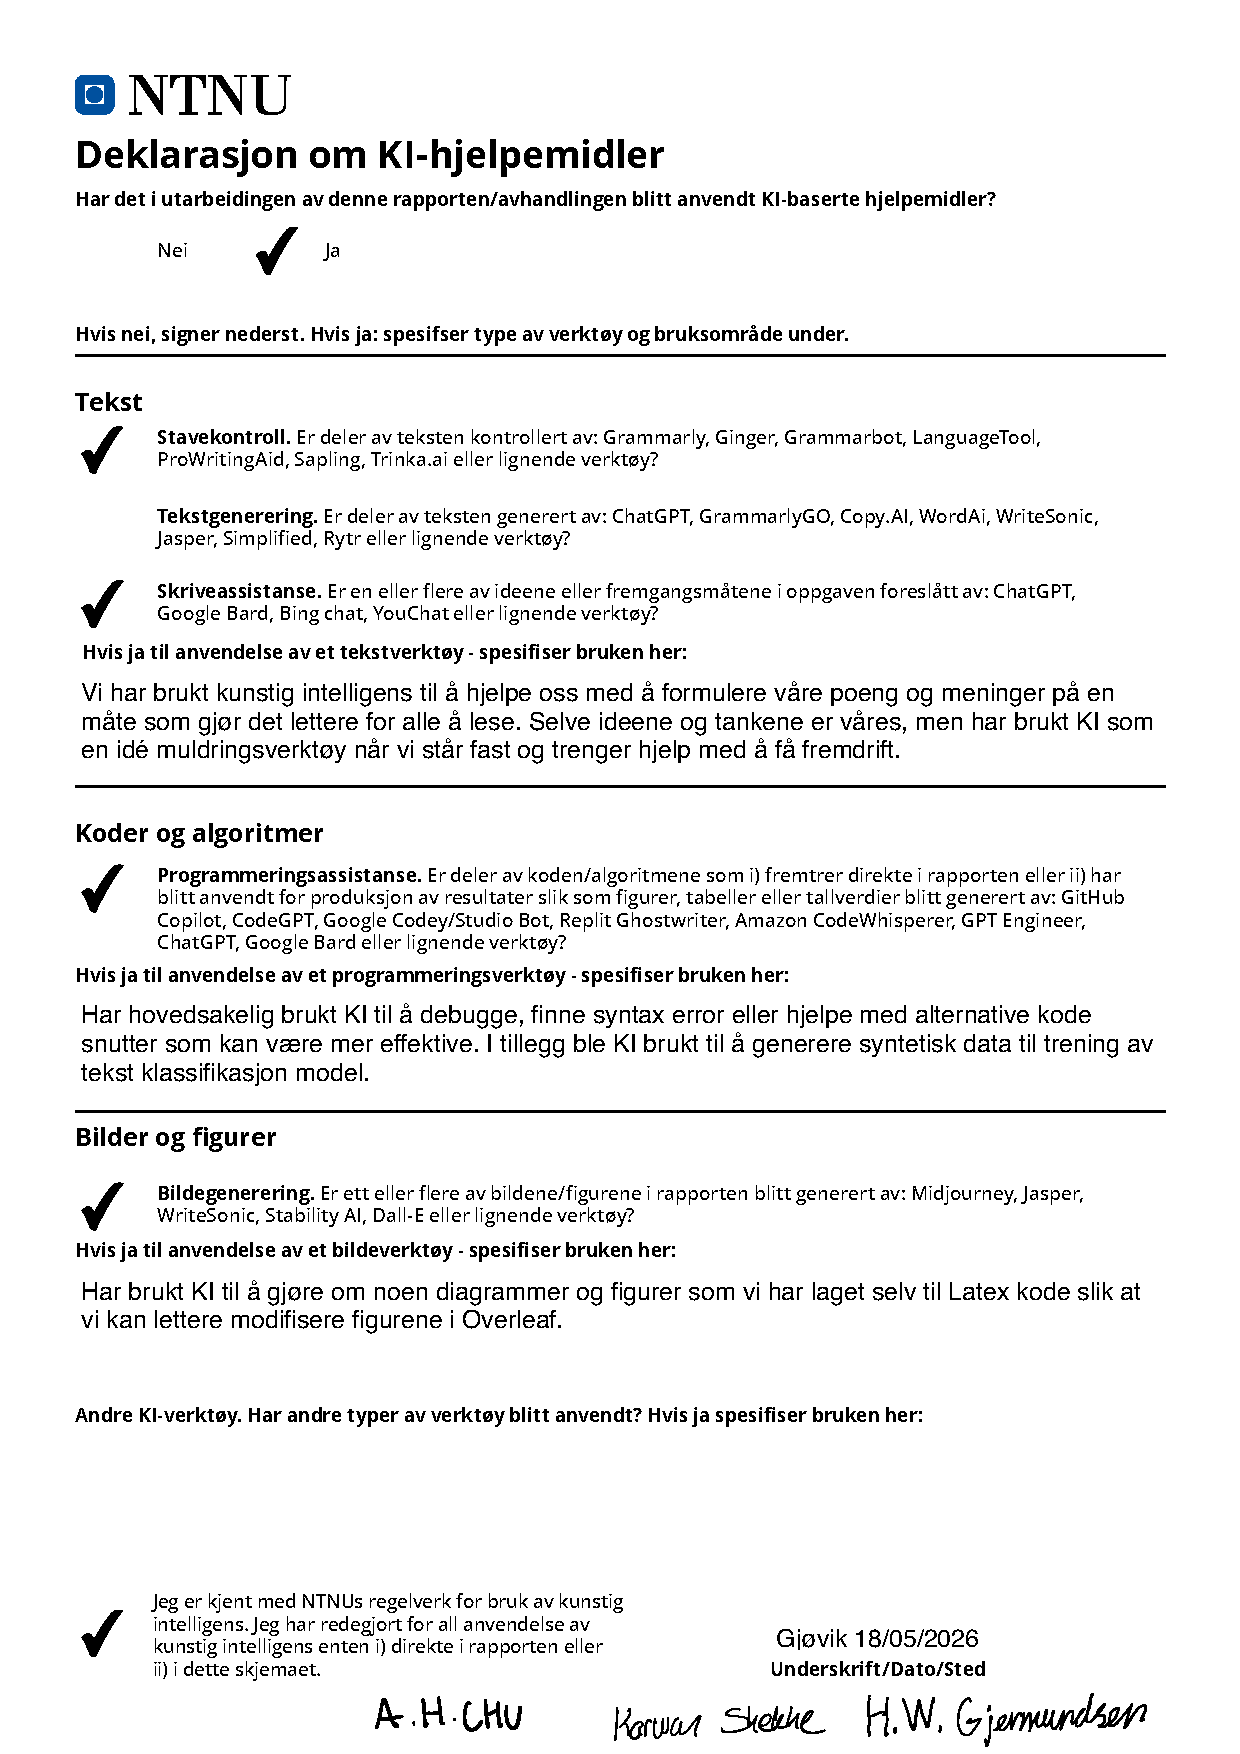
\includepdf[pages=-]{appendices/KI_Deklerasjon_BachelorV2026.pdf}
\chapter{Oppgave 37}
\label{app:oppgave37}

\section*{Assignment Information}

\begin{tabular}{@{}ll@{}}
\textbf{Assignment title:} & AI-based removal of sensitive information from images and video \\
\textbf{Company:} & Safe Media AI AS \\
\textbf{Contact person:} & Jon Yngve Hardeberg \\
\textbf{E-mail:} & jon@safemediaai.no \\
\textbf{Study program:} & DIGSEC, BIDATA, BPROG \\
\end{tabular}

\section*{Description}

Photographs and videos are widely used in society to document various locations and events. Examples include surveillance cameras, street view solutions from map providers, documentation of crime scenes, and journalistic photographs in public places. For privacy reasons, it is often necessary to remove sensitive information, such as recognizable faces, readable text, and metadata, from such photographs before they can be made publicly available. This process is sometimes called redacting, and doing it manually using tools such as Photoshop can be tedious and may also present several challenges. AI-based software solutions of various levels of quality are currently being proposed in the marketplace.

Safe Media AI AS has currently developed a powerful AI-based platform for redacting text-based documents. They would like to enhance their product portfolio by providing competitive solutions for redacting images and possibly videos. The overall goal of the project is to design, develop, and evaluate a complete and user-friendly solution for this, supported by state-of-the-art AI models.

\section*{Project Goals}

The project goals include:

\begin{itemize}
    \item Survey related state of the art from both research literature and available products.
    \item Develop a software solution which can identify and remove/redact sensitive content in images and videos.
    \item Ensure that the solution is compatible with existing tools developed by Safe Media AI AS, supports various file formats, and includes both fully automatic AI-based and user-friendly interactive methods.
    \item Ensure that the proposed solution is well justified with regards to state-of-the-art solutions, has a certain degree of novelty, follows strict standards for security and privacy, and is evaluated both quantitatively and qualitatively.
\end{itemize}

\chapter{In-depth User Interface and User Experience Design}
\label{app:depth_ui_ux}

This appendix provides additional documentation for the user interface design process described in Chapter~\ref{user_interface_and_usability}. While the main chapter focuses on the final interface and its usability principles, this appendix presents the earlier design iterations, prototype development, MVP stage, and additional interaction considerations that informed the final design.

\section{Design Methodology and Principles}

Development of the user interface followed an iterative design process, where layout, interaction patterns, and workflow structure were gradually refined throughout the project. Iterative design is widely recommended in user interface development because it allows teams to evaluate design decisions and improve solutions based on testing and practical experience \cite{hartson2012ux}. This approach allowed the design to evolve alongside the technical implementation while maintaining focus on usability and user control.

\methodheading{Iterative and Agile Design Process}

An agile development approach was used, where design and implementation were carried out in parallel. As new features were introduced, the interface was continuously adjusted to support the expanding functionality of the system. The approach aligns with Agile UX practices, where interface decisions are refined through incremental improvements rather than finalized early in development \cite{gothelf2022leanux}. 

Initial wireframes were created in Figma to explore layout and interaction flows before implementation (Appendix~\ref{fig:prototype_loaded}). Wireframing allows designers to quickly test ideas before committing to development \cite{hartson2012ux}. They were used to define the main workflow.

A functional prototype was then implemented to evaluate interaction patterns and identify usability issues in a practical environment. After the prototype stage, the design was refined into a minimum viable product (MVP), where core system functionality was integrated into the interface (Appendix~\ref{fig:mvp_detection}). The interface was also influenced by Safe Media AI's existing system, allowing users familiar with that platform to encounter recognizable layout structures and interaction patterns. This helped support consistency and reduced the learning curve for potential users.

\methodheading{Core Design Principles}

User control over automated processes was a central design principal. Since detection is performed by machine learning models, users must be able to verify, adjust, and override automated results when necessary \cite{hartson2012ux}. The interface supports this through manual highlighting, adjustment of detection settings, removal of incorrect detections, and customization of redaction methods.

Simplicity was also prioritized to reduce cognitive load and allow users to focus on identifying and redacting sensitive information \cite{norman2013design}. The interface therefore emphasizes essential functionality while avoiding unnecessary complexity. This was especially important because users must inspect visual content carefully and should not be distracted by unrelated interface elements.

Visual feedback was prioritized to help users understand system state and detection outcomes \cite{norman2013design}. Detection results are displayed directly on the media using labelled bounding boxes, enabling immediate interpretation of what the system has identified. Progress indicators and visible processing states further help users understand when the system is working.

Consistency across components improves usability and learnability \cite{nielsen2020progressive}. Toolbars, panels, and controls follow predictable patterns, making the interface easier to navigate. In addition, alignment with familiar structures from Safe Media AI's existing system supports recognition for users already accustomed to that platform, while still allowing SafeVision to introduce functionality specific to visual media redaction.

\section{Design Evolution}

The interface evolved through several stages, beginning with simple wireframes and later progressing into a prototype, MVP, and final interface. Each stage was used to explore layout, interaction flow, and the relationship between automated detection and manual user control.

The design was also influenced by Safe Media AI's existing interface. This was done to preserve familiar layout structures and interaction patterns for users already accustomed to that platform, while adapting the workflow to the specific needs of visual media redaction.

The early design stages focused on establishing the main workflow: uploading media, running detection, reviewing results, and applying redaction. Later iterations expanded this into a more complete workspace that supported manual correction, configuration options, visual feedback, and video processing.

\subsection{Initial Design}

Based on the initial requirements and project scope, the first interface design only needed to support a limited set of core functions: uploading an image, detecting sensitive information, and redacting detected content. Because of this limited scope, it was determined early in the design phase that the application did not require multiple pages, pop-up dialogs, or additional navigation views. Instead, the full workflow could be contained within a single interface, allowing users to complete the main redaction process in one place.

The initial interface was centered around a main interaction area for the uploaded image. Before upload, the interface presented a minimal layout with a central upload button, as shown in Figure~\ref{fig:prototype_empty}.

\begin{figure}[H]
\centering

\includegraphics[width=0.8\textwidth]{figures/images/chapter-6/figmasketch3.png}
\caption{Initial interface before an image is uploaded.}
\label{fig:prototype_empty}
\end{figure}

After upload, the layout adapts to include interaction features. The upload button moves to the top, while the central area becomes the image viewer.

A file list is displayed on the left, and control buttons below the viewer allow detection, redaction, and highlighting. This placement maintains a clear connection between the image and available actions, as shown in Figure~\ref{fig:prototype_loaded}.

\begin{figure}[H]
\centering
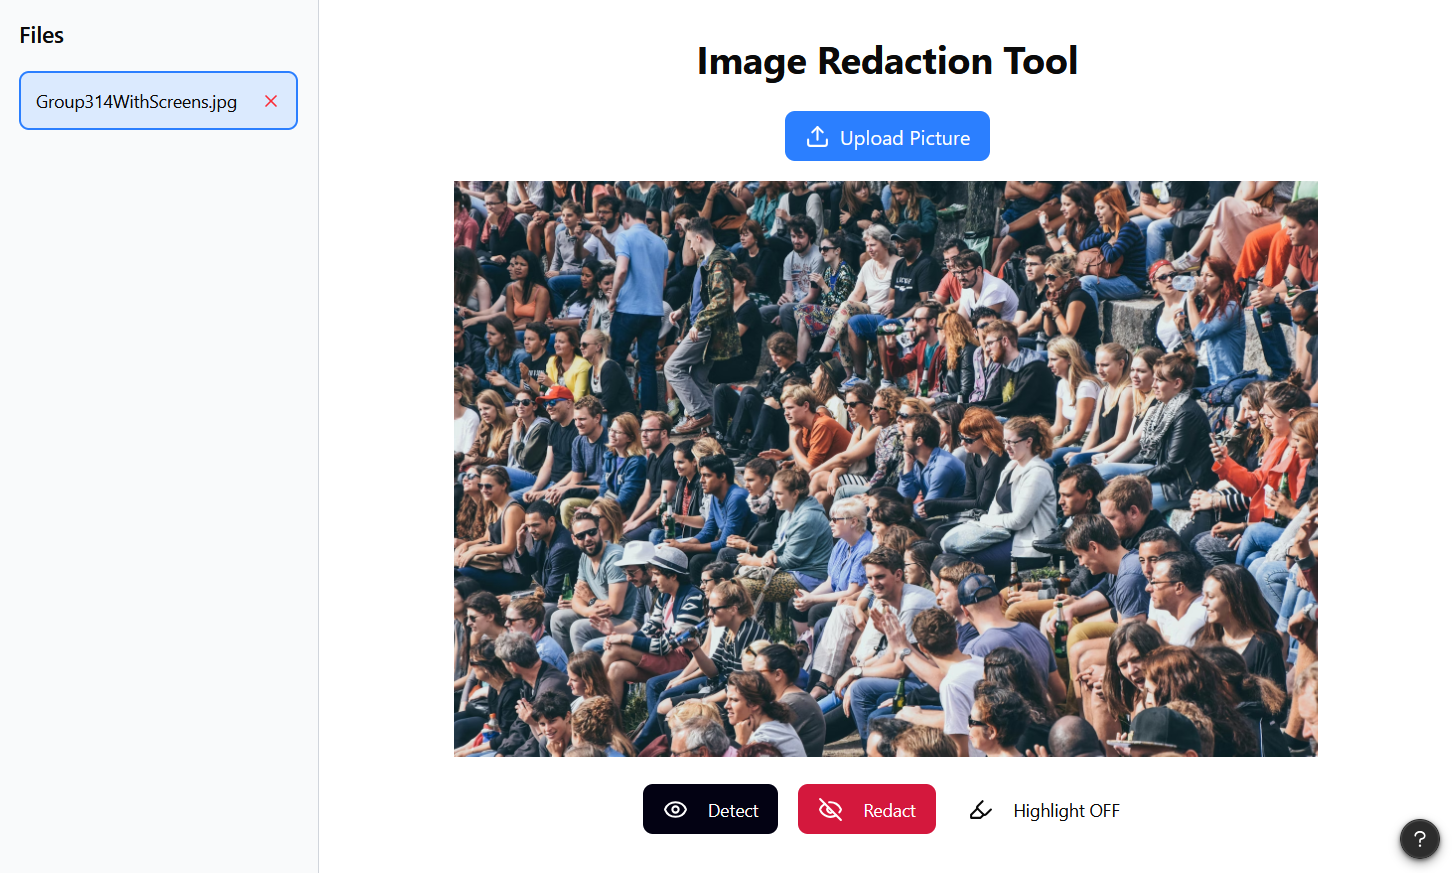
\includegraphics[width=0.8\textwidth]{figures/images/chapter-6/figmasketch4.png}
\caption{Prototype interface after an image has been uploaded.}
\label{fig:prototype_loaded}
\end{figure}

This design provides a clear workflow where users upload an image, run detection, and apply redaction.

\subsection{Prototype}

The prototype was developed in a separate repository to explore layout and interaction patterns without affecting the main system.

Key components such as a sidebar, navigation bar, and central viewer were introduced to structure the interface and organize available tools.

\begin{figure}[H]
\centering
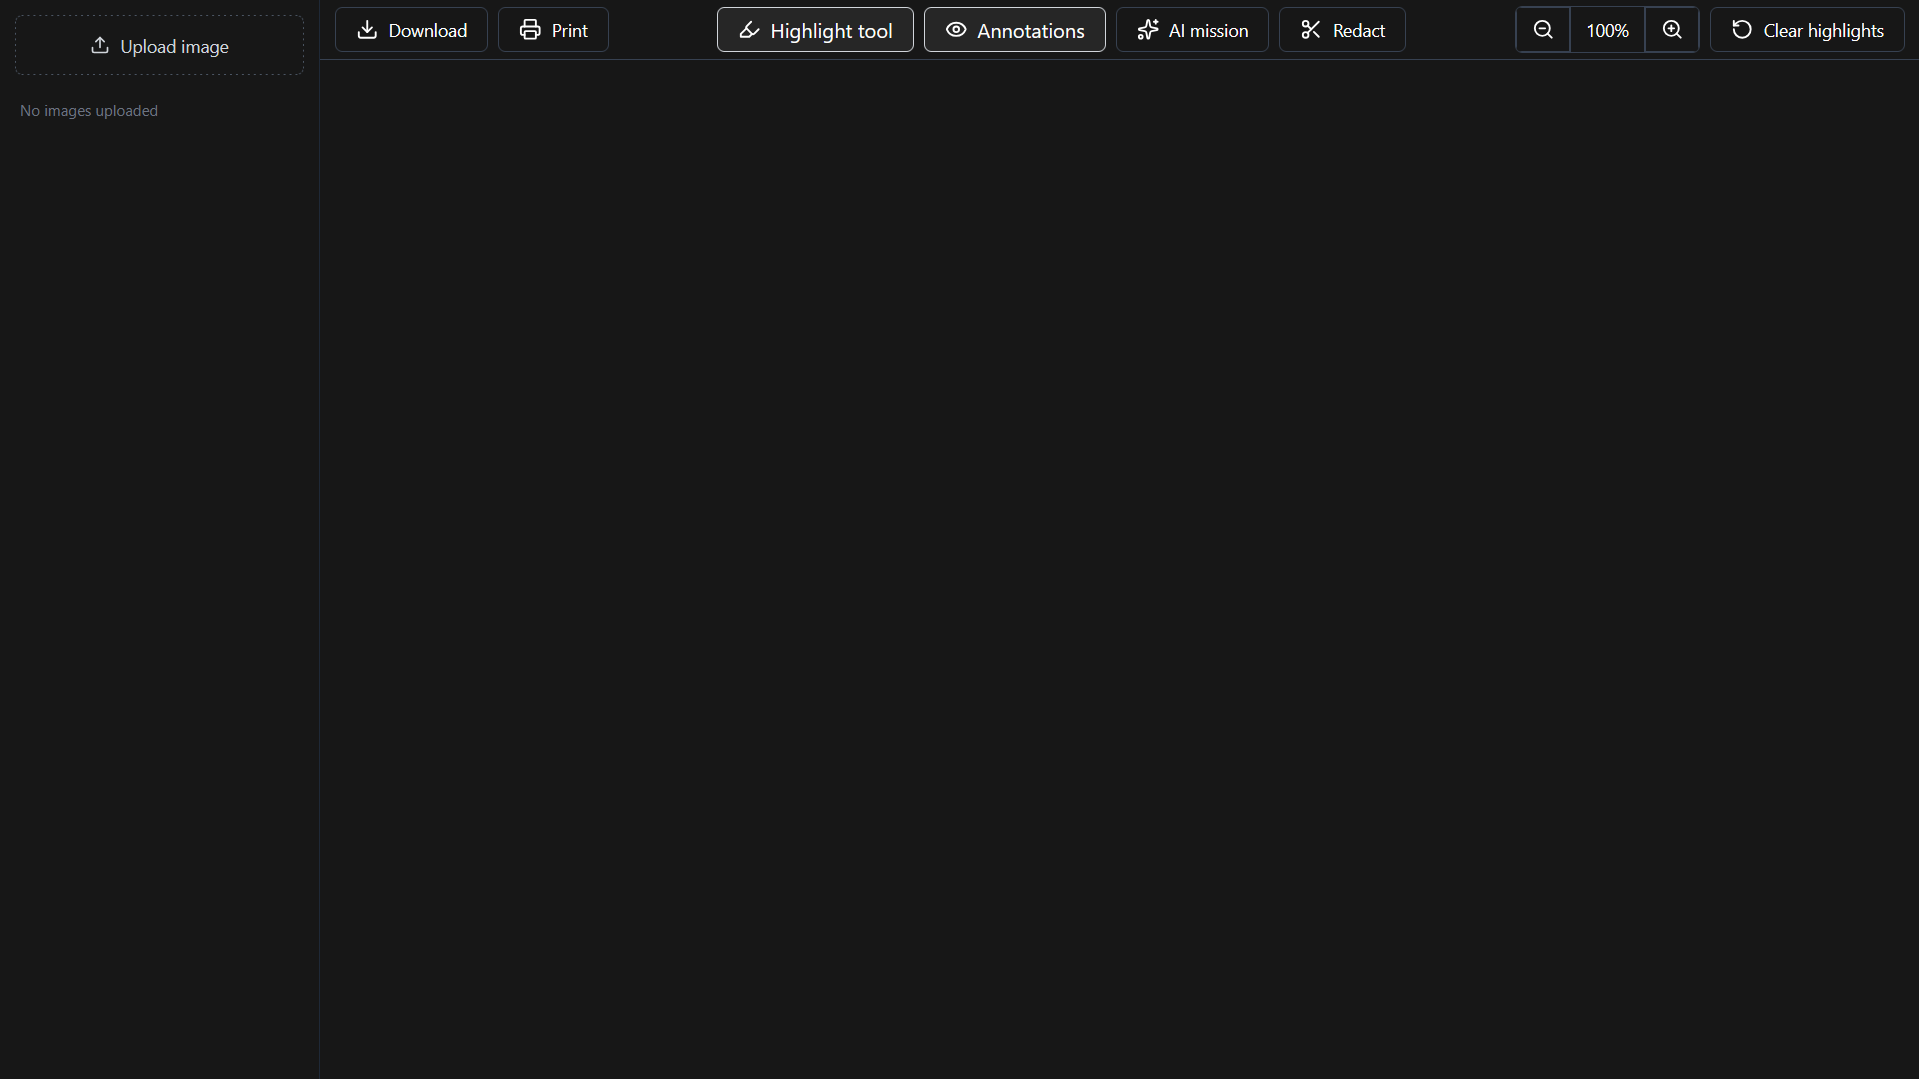
\includegraphics[width=0.8\textwidth]{figures/images/chapter-6/prototype1.png}
\caption{Prototype interface showing the sidebar, navigation bar, and image viewer.}
\label{fig:prototype_overview}
\end{figure}

Some elements were included for layout testing only, such as the \textit{AI Mission} and \textit{Redact} buttons.

The prototype also introduced manual highlighting, allowing users to mark regions directly within the viewer.

\begin{figure}[H]
\centering
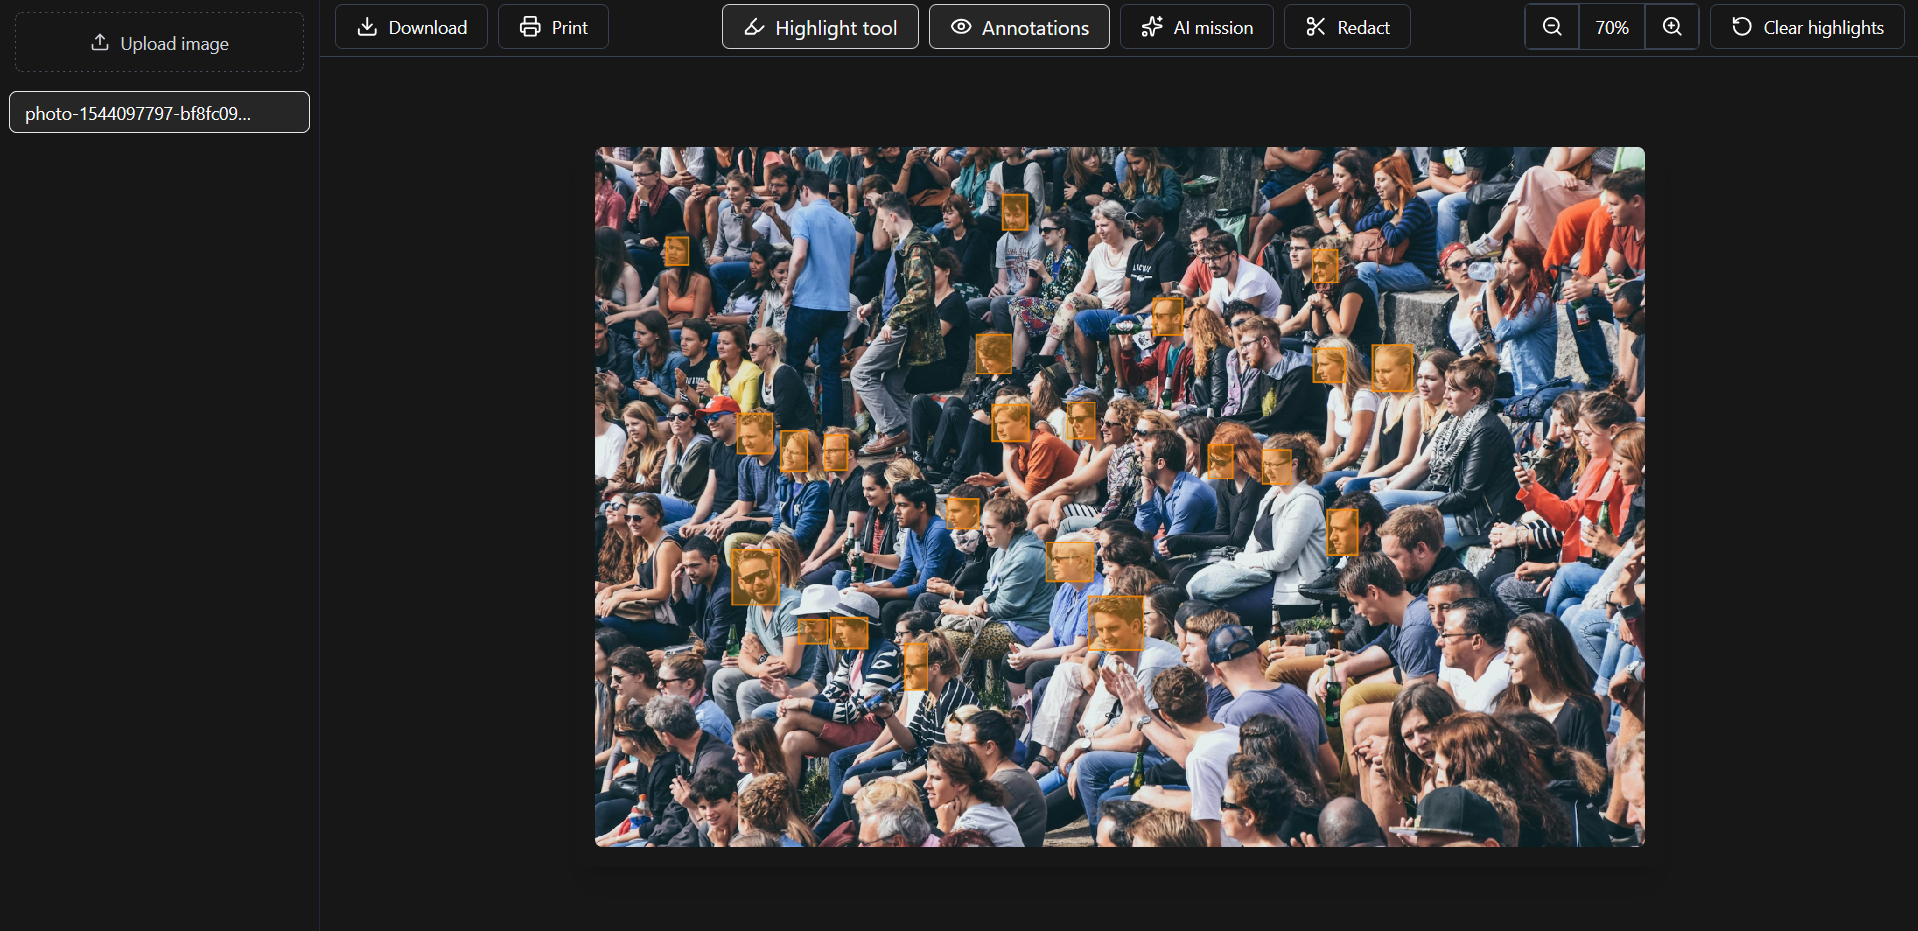
\includegraphics[width=0.7\textwidth]{figures/images/chapter-6/prototype3.png}
\caption{Prototype example showing manually highlighted regions.}
\label{fig:prototype_detection}
\end{figure}

\subsection{MVP Design Iteration}

The MVP introduced functional backend integration while preserving the basic prototype layout, including the sidebar structure and central viewer. Previously inactive interface elements were connected to system functionality, allowing users to run automatic detection and view results as bounding boxes.

At this stage, the interface also explored support for multi-page PDF documents. This allowed users to navigate pages within the same workspace. However, as the project scope evolved, PDF support became less central and the interface was later refocused around image and video redaction.

This iteration was important because it connected the visual interface to actual detection functionality. It also confirmed the need for a human-in-the-loop workflow, where automated detection results are shown visually and can be reviewed before redaction.

\begin{figure}[H]
\centering
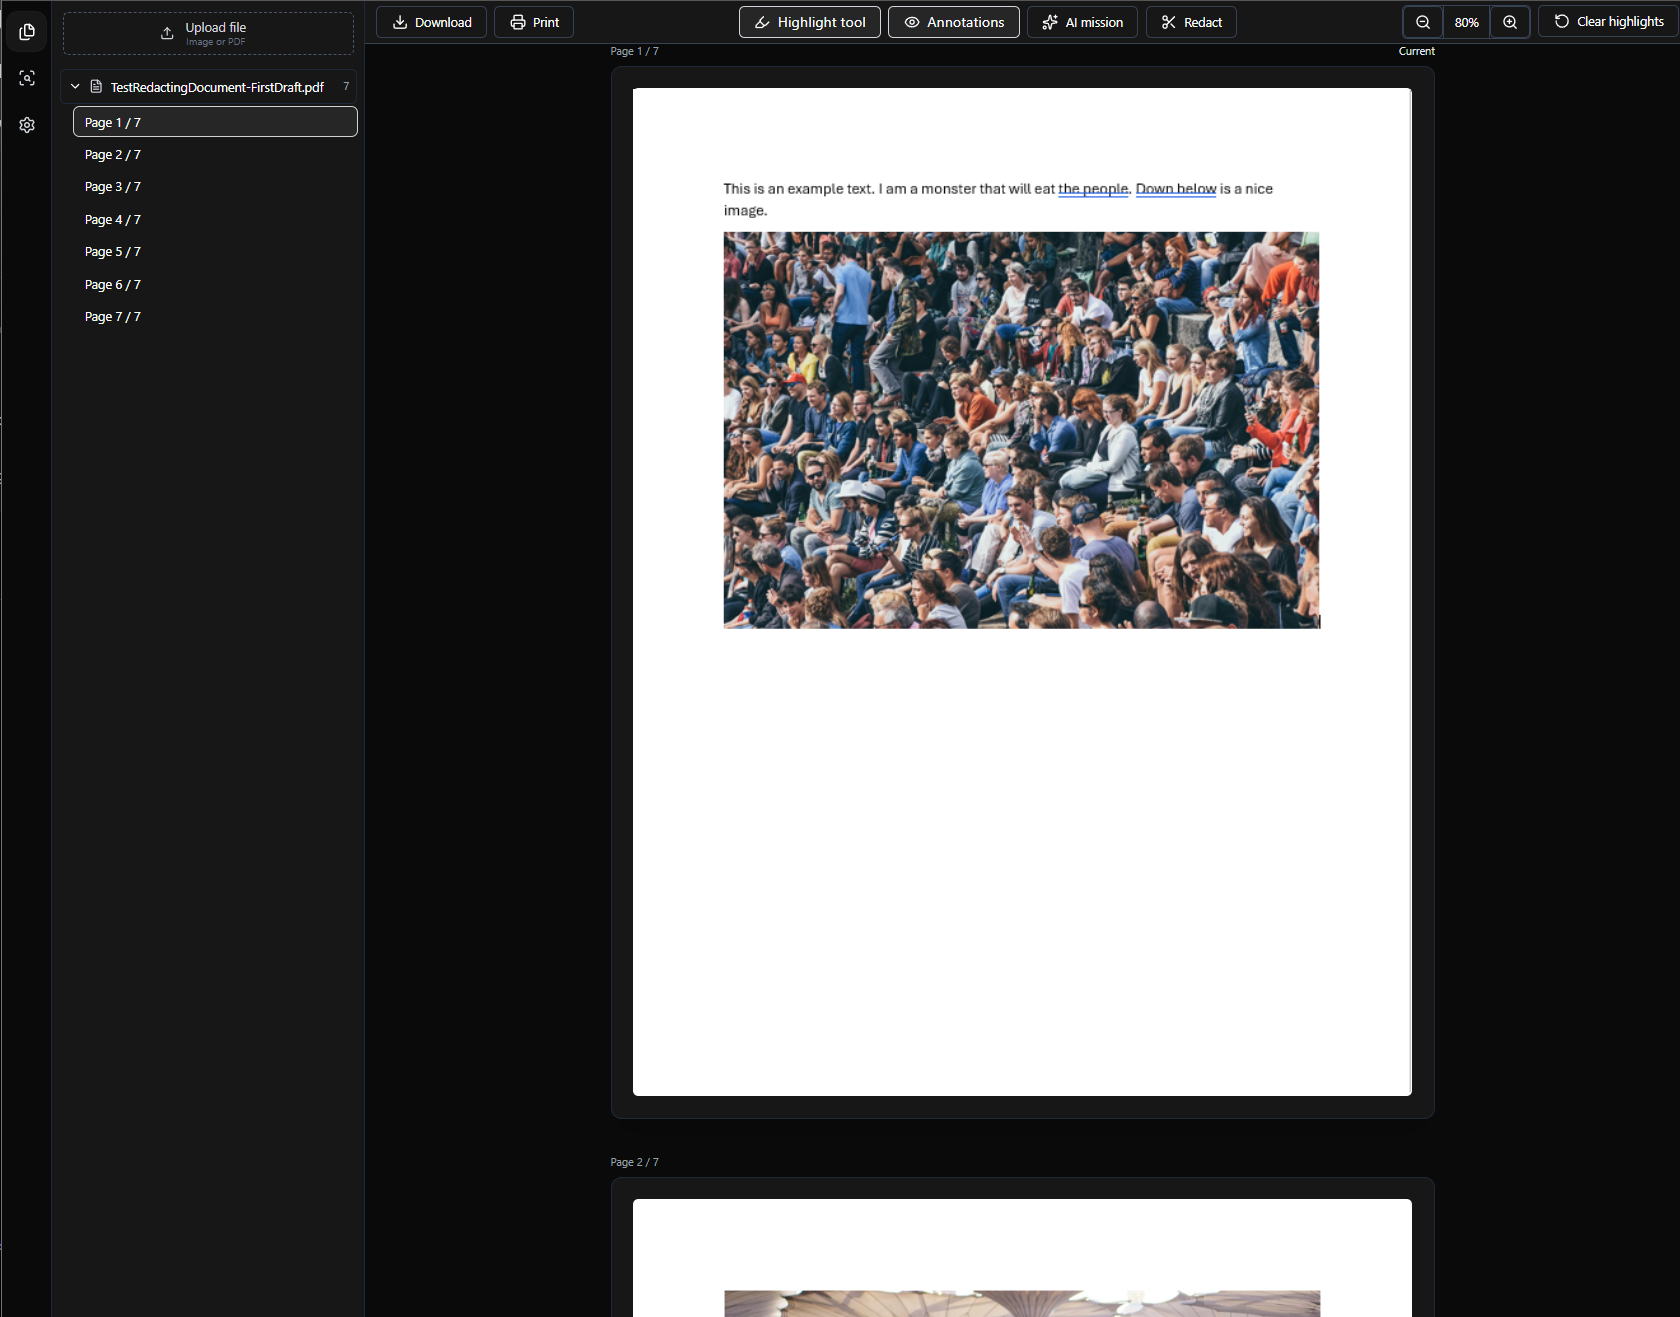
\includegraphics[width=0.8\textwidth]{figures/images/chapter-6/mvp1.png}
\caption{MVP interface showing the document viewer and navigation structure.}
\label{fig:mvp_overview}
\end{figure}

Support for multi-page PDF documents was also introduced, allowing users to navigate pages within the same interface.

\begin{figure}[H]
\centering
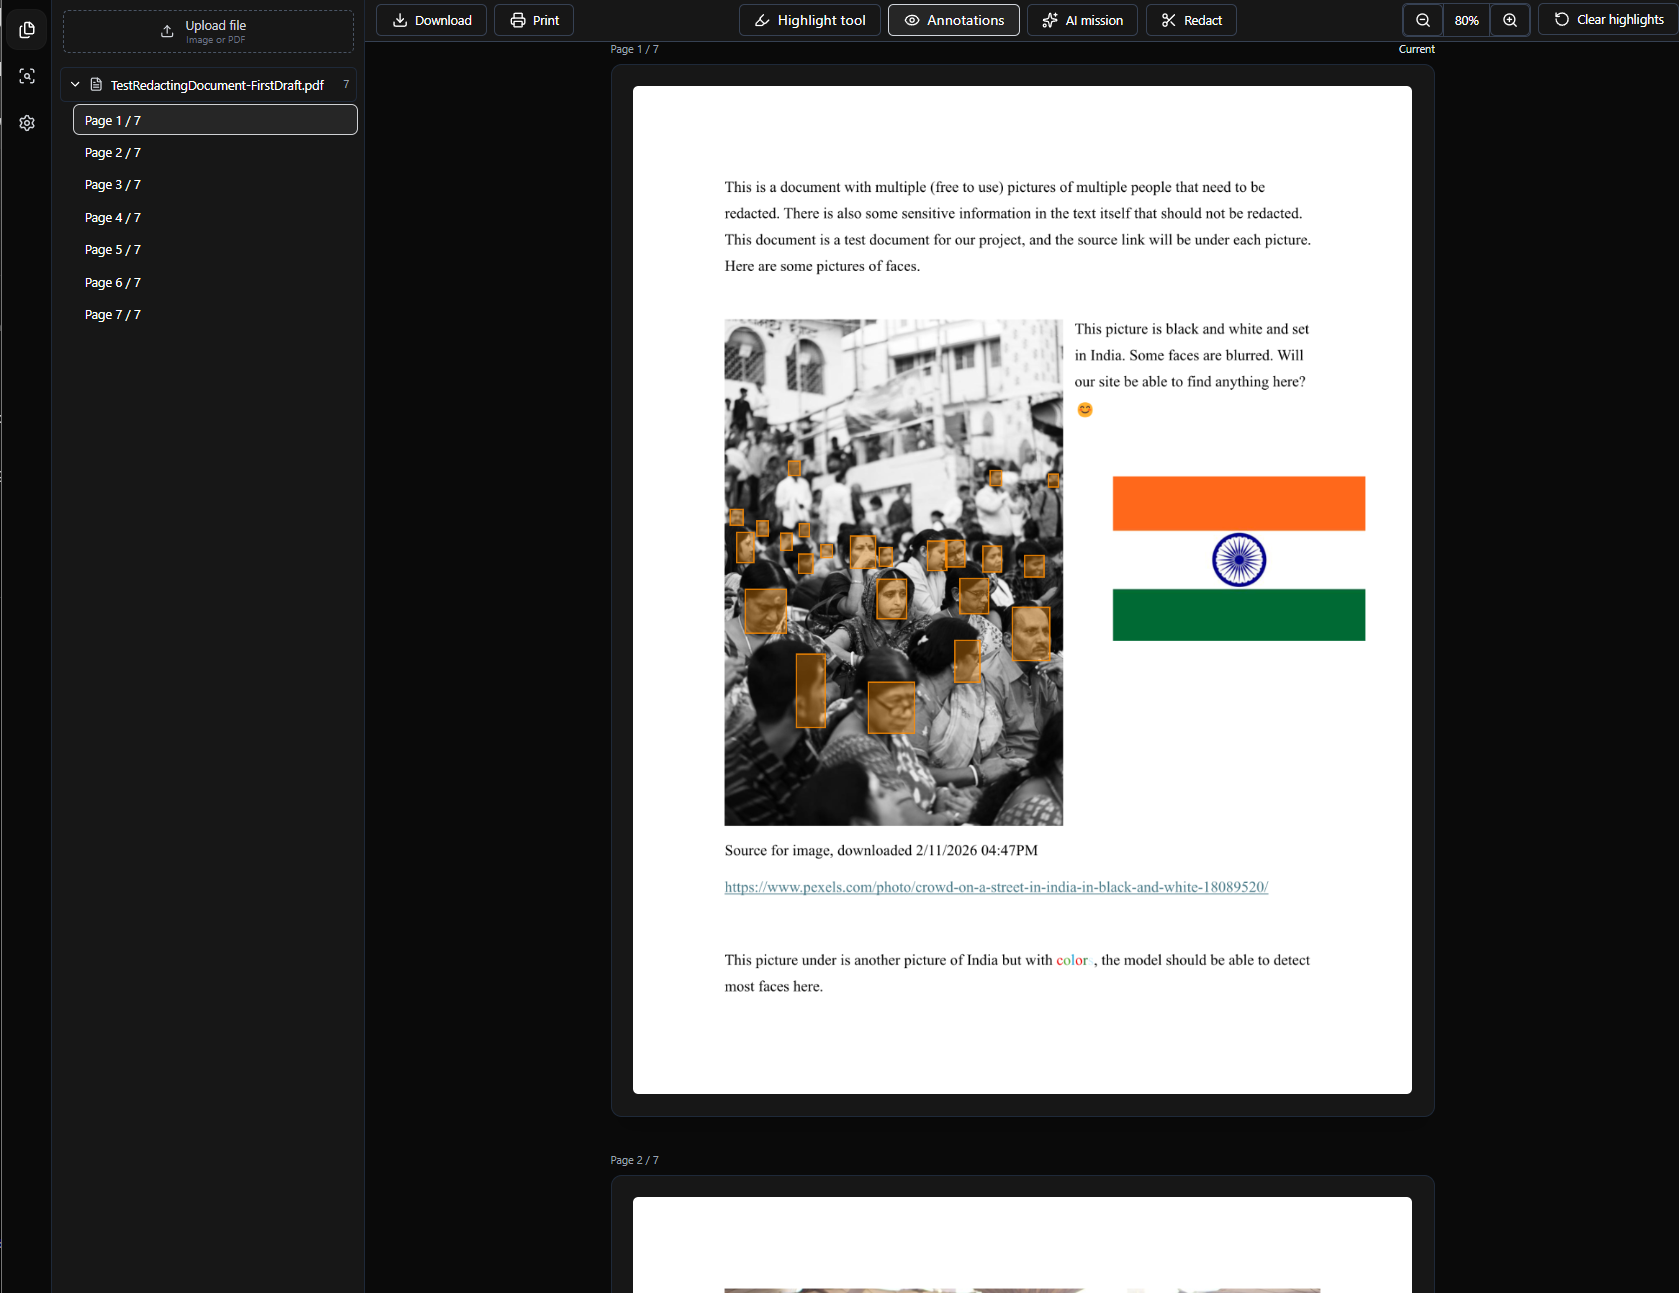
\includegraphics[width=0.8\textwidth]{figures/images/chapter-6/mvp2.png}
\caption{Detection results displayed using bounding boxes.}
\label{fig:mvp_detection}
\end{figure}

This iteration integrates automated detection with manual interaction, enabling users to verify and refine results before applying redaction.

\subsection{Final Design Direction}

The final design refined the interface into a focused workspace for image and video redaction. Compared with earlier iterations, the layout was simplified to reduce visual complexity and improve usability. The final interface retained the central viewer and side-panel structure, but reorganized controls so that upload, identification, review, correction, and redaction could be completed in a more natural sequence.

As the project evolved, support for PDF workflows was reduced, while video processing capabilities were introduced. This required the interface to support temporal media through playback controls, frame-based inspection, and detection overlays on video frames. A Terms of Service component was also implemented to address privacy and data protection requirements before users interact with the system.

The final interface and its components are described in the main text in Section~\ref{user_interface_and_usability}. This appendix therefore focuses on documenting the design progression that led to the final solution.

\section{Usability and Interaction Design}

This section focuses specifically on the interaction between the user and the machine learning-based detection and redaction functionality. While the interface includes several general usability features, the primary objective of the system is to support a human-in-the-loop workflow. Therefore, the usability discussion is centered on how users interact with detection results, verify automated outputs, and apply redaction.

\subsection{Interaction with Detection Results}

The core interaction in the system occurs within the document viewer, where detection results are presented directly on the image using bounding boxes. This allows users to immediately interpret the output of the detection models and understand which regions have been identified as potentially sensitive.

Since machine learning models are not perfectly accurate, it is essential that users can validate these results. The interface therefore allows users to manually adjust bounding boxes, remove incorrect detections, and add new regions if necessary. This ensures that the final outcome is not solely dependent on automated predictions, but can be refined through user input.

By combining automatic detection with manual correction, the system supports a more reliable and controllable redaction process.

\subsection{Detection Configuration and Control}

Users are able to control the detection process by selecting which categories of sensitive information to detect. This allows the system to be adapted to different use cases, where only specific types of content may be relevant.

Providing this level of control reduces unnecessary visual clutter and improves usability by ensuring that users only see relevant detection results. It also allows users to tailor the system behavior to the specific context of the document or image being processed.

\subsection{Redaction Interaction}

Once detection results have been reviewed, users can apply redaction directly within the interface. Multiple redaction methods are available, including black box redaction, blur, and pixelation.

Allowing users to select and adjust redaction methods provides flexibility in how sensitive information is concealed. For example, blur and pixelation may preserve some visual context, while solid redaction completely removes visibility. This enables users to choose the most appropriate method depending on the sensitivity of the content.

The integration of redaction controls within the same workspace as detection results ensures a seamless workflow, where users can move directly from analysis to action without changing context.

\subsection{Visual Feedback for Verification}

Clear visual feedback is essential when interacting with automated detection systems. In the interface, detection results are displayed as overlays on the document, allowing users to quickly assess model outputs.

This immediate feedback supports rapid verification, as users can visually confirm whether detected regions correspond to actual sensitive content. Any inaccuracies can then be corrected before redaction is applied.

By providing continuous visual feedback throughout the workflow, the interface helps users maintain awareness of system behavior and increases confidence in the final result.

\subsection{Accessibility Considerations}

Accessibility considerations were integrated into the interaction design to support effective use of detection and redaction tasks over extended periods. Since the system requires detailed visual inspection, emphasis was placed on reducing visual strain and enabling flexible interaction.

Visual accessibility is supported through dark and light modes, allowing adaptation to different lighting conditions. Users can also customize highlight colors for detection results and manual annotations, improving readability and distinction between detection categories. Zoom functionality further enables detailed inspection of small regions without losing context.

Interaction accessibility is addressed through flexible input methods. Keyboard shortcuts support efficient interaction during repetitive tasks, while undo and redo functionality allow users to safely adjust detection results and redaction without risk of permanent errors.

Together, these features improve usability, flexibility, and efficiency in the human-in-the-loop redaction workflow.

\methodheading{Terms of Services}
\label{app:terms_of_service}

A Terms of Service dialog was included in the final interface to clarify user responsibility, acceptable use, data handling, and the limitations of automated redaction. The text below summarizes the terms shown to users before processing content in \gls{SafeVision}.

\begin{enumerate}
    \item \textbf{Operator and contact:} The service is operated by An Hoang Chu, Karwan Shekhe, and Henrik Weflen Gjermundsen. Contact: henrik.w.gjermundsen@gmail.com.

    \item \textbf{What the service does:} The service provides automated detection and redaction functionality to help redact images. Automated detection may be inaccurate or incomplete.

    \item \textbf{User responsibilities and acceptable use:} Users confirm that they have the necessary rights and a valid legal basis to upload and process any personal data contained in the content they submit. Users must not upload unlawful content or content that infringes the rights or privacy of others. Users must not upload content involving children or other vulnerable individuals unless they are legally authorised to do so. Users are responsible for reviewing the output before sharing, publishing, or otherwise using it, because redaction may be imperfect. Access may be blocked or restricted if there is reasonable belief that the service is being misused or used unlawfully.

    \item \textbf{How images are processed, stored, and deleted:} When an image or document is uploaded, it is transmitted to the backend servers and processed by the system to detect sensitive content and apply redaction. The servers are hosted on infrastructure provided by Google Cloud. Uploaded images and redacted outputs are not stored permanently. Uploads are used only to generate the result and are deleted after the result is returned, although transient technical handling may occur during processing and delivery. Uploaded content is not used to train or improve the model.

    \item \textbf{Browser-stored backtracking and cached box data:} To support editing features, the web application stores derived detection data in the user's browser on the user's device. This may include bounding-box coordinates, image dimensions, and related redaction or editing state. The service uses an in-memory undo and redo history during the session, as well as local browser storage or cache to restore detected boxes and editing state when the user revisits the site. This browser-stored data does not include the original uploaded image. Users can remove this data at any time by clearing the site's data in their browser.

    \item \textbf{Logging:} The service does not intentionally log or retain uploaded image content. Some infrastructure-level operational data may be processed transiently to deliver the service.

    \item \textbf{Rights and complaints:} For questions or data protection requests, users can contact henrik.w.gjermundsen@gmail.com. Users may also lodge a complaint with their supervisory authority, Datatilsynet.

    \item \textbf{Disclaimer:} The service is provided ``as is'' and ``as available.'' The system does not guarantee that all sensitive content will be detected or redacted. Users are responsible for verifying outputs before sharing or publishing. Nothing in these terms limits liability where such limitation is not permitted by law.
\end{enumerate}



% appendices/custom_detection_model_evaluation.tex

\chapter{Detailed Evaluation of Custom-Trained Detection Models}
\label{app:custom_model_evaluation}

\section{Barcode Detection}
\label{app:barcode_detection}
This section provides detailed training and evaluation results for the final
barcode detection model.

\subsection{Training Setup}

\begin{table}[H]
\centering
\begin{tabular}{lccc}
\toprule
Total Images & Training & Validation & Testing \\
\midrule
15731 & 12583 & 1572 & 1576 \\
\bottomrule
\end{tabular}
\caption{Dataset split used for the barcode detection model.}
\label{tab:bc_training_split}
\end{table}

\subsection{Training Configuration}

\begin{table}[H]
\centering
\caption{Training configuration for the final barcode detection model.}
\label{tab:barcode_training_config}
\scriptsize
\renewcommand{\arraystretch}{1.05}
\begin{tabular}{lp{7cm}}
\toprule
\textbf{Parameter} & \textbf{Value} \\
\midrule
Architecture & YOLOX-S \\
Input Resolution & $960 \times 960$ \\
Batch Size & 4 \\
Max Epochs & 150 \\
No-Aug. Epochs & 15 \\
\midrule
\textit{Optimization} & \\
Base Learning Rate & 0.01 / 64 \\
Warmup Epochs & 5 \\
Min LR Ratio & 0.05 \\
Optimizer & SGD \\
\midrule
\textit{Augmentation} & \\
Mosaic / Mixup & 0.0 / 0.0 \\
Color / Flip & 0.5 / 0.5 \\
Rotation / Shift / Shear & 5.0 / 0.05 / 1.0 \\
\midrule
\textit{Hardware} & \\
GPU Model & RTX 4080 \\
\bottomrule
\end{tabular}
\end{table}







\subsection{Training Behaviour}

\begin{figure}[H]
\centering

\begin{subfigure}{0.50\textwidth}
\centering
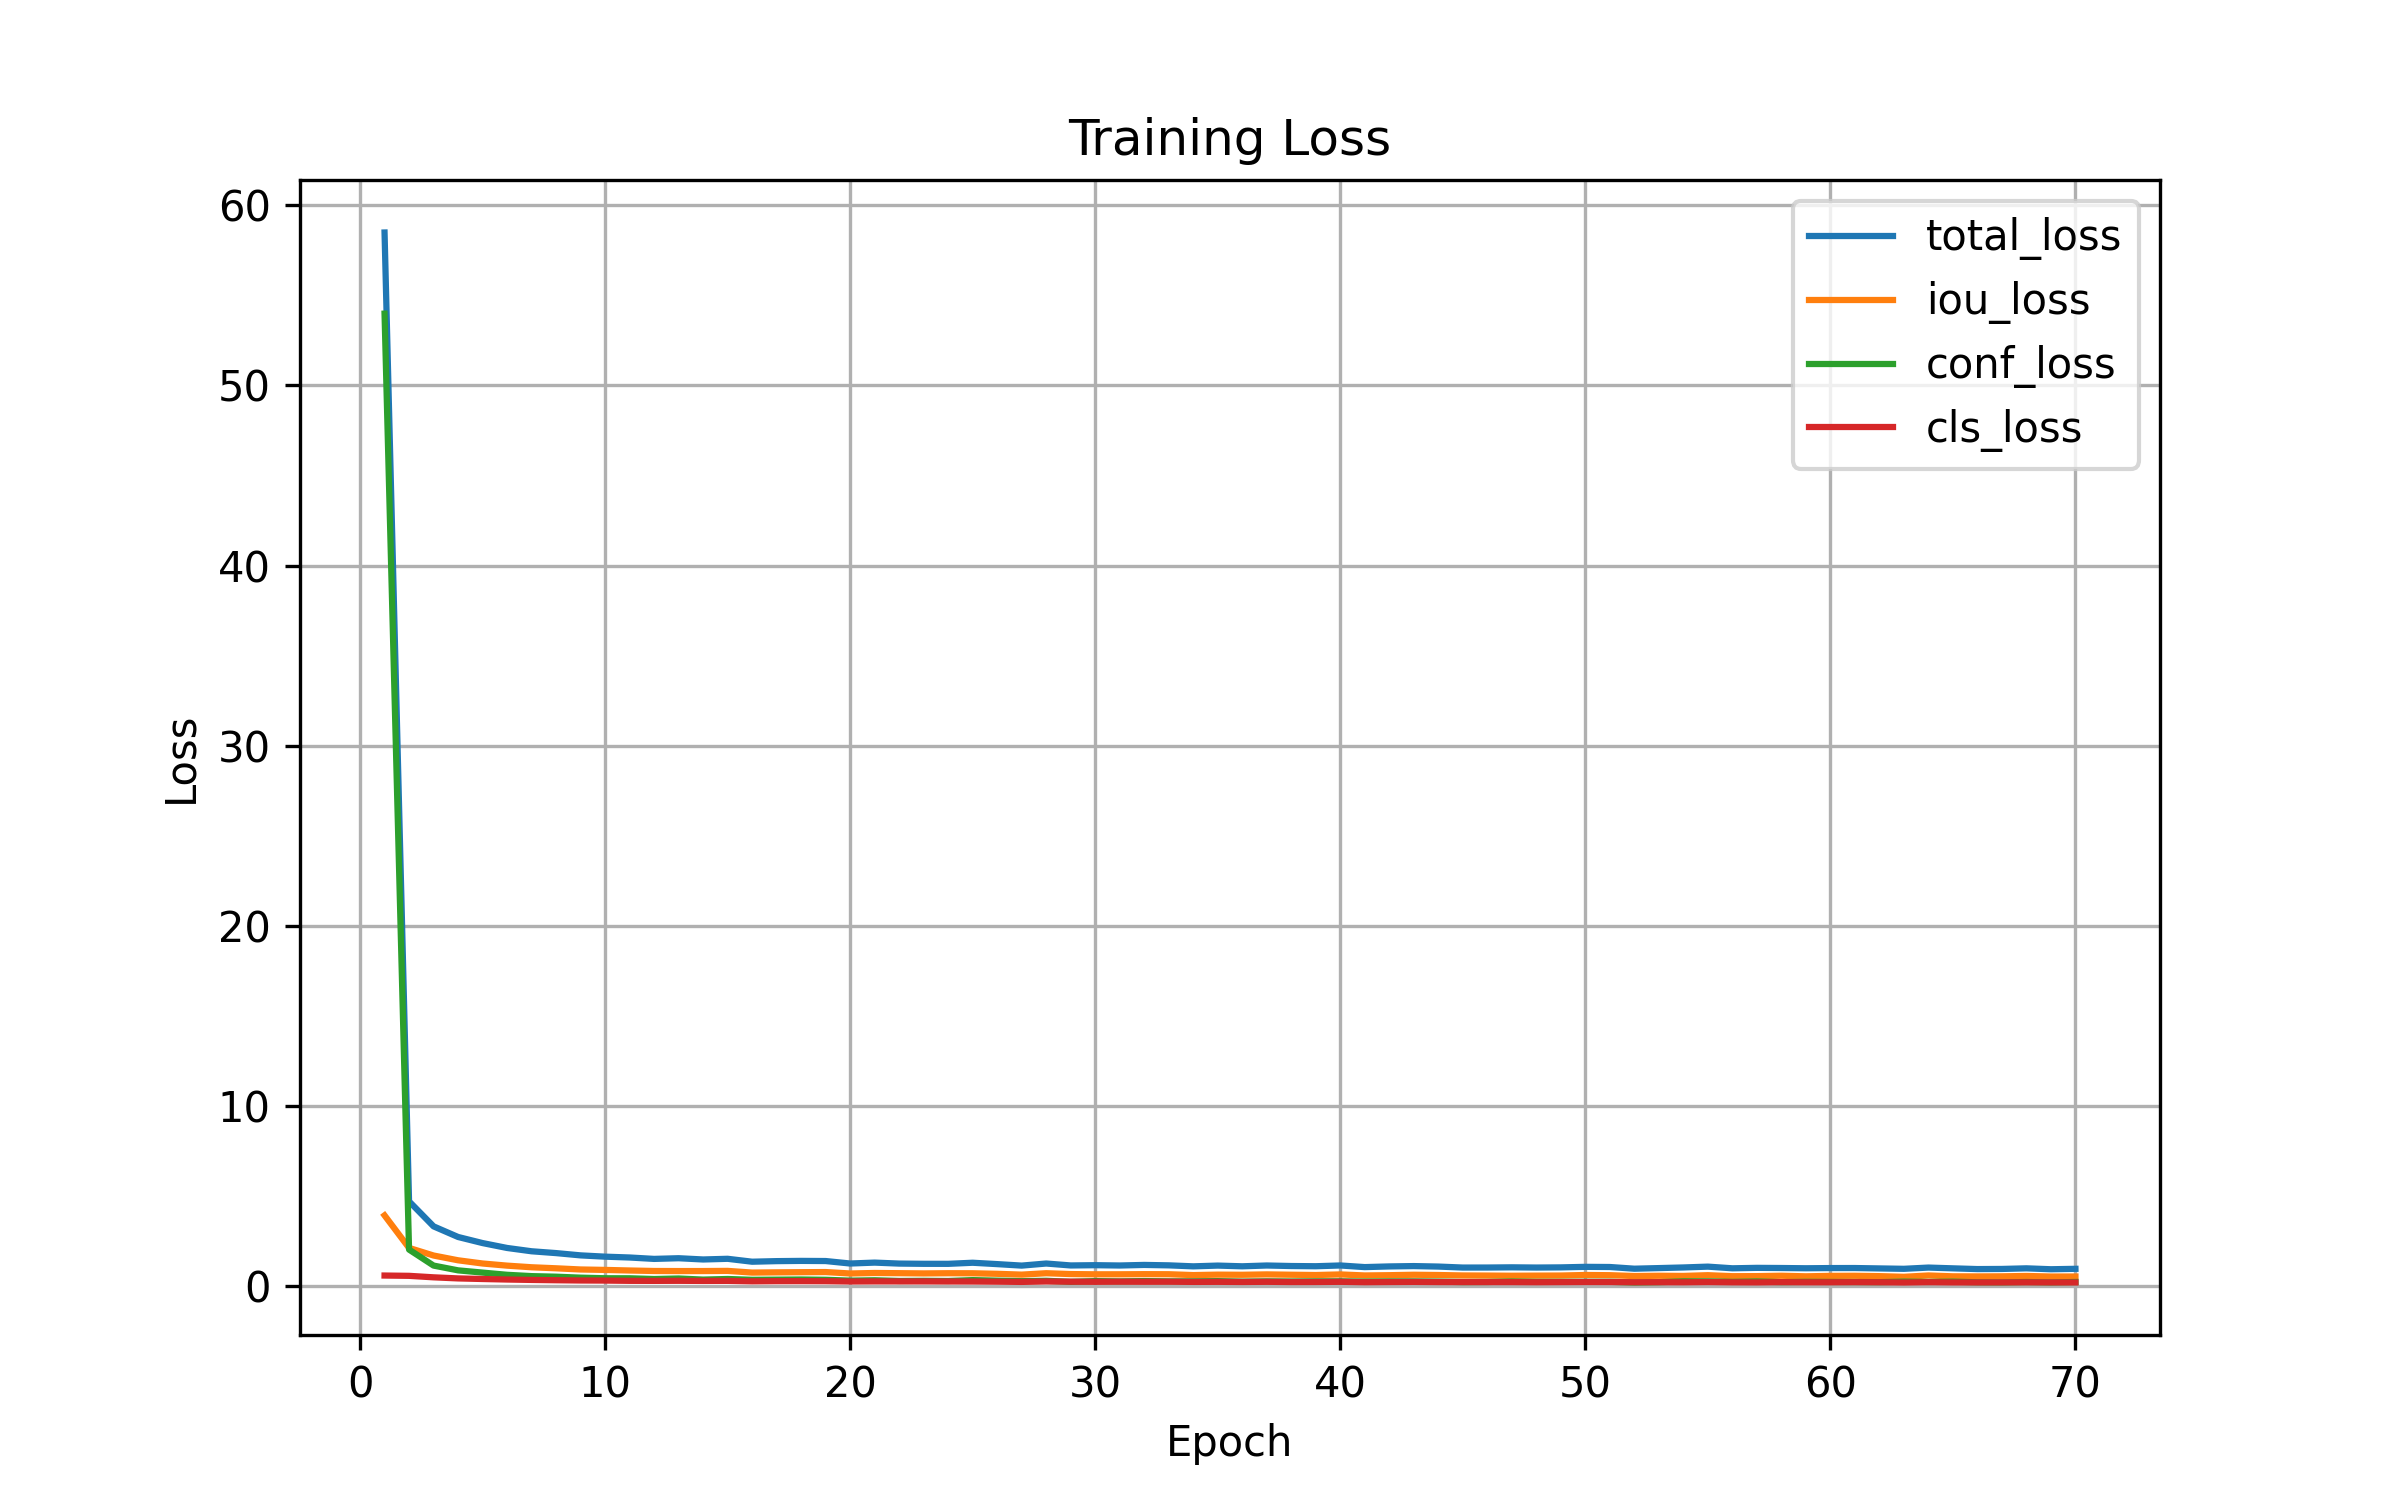
\includegraphics[width=\linewidth]{figures/images/chapter-11/qr-bar/v0/loss_curve.png}
\caption{Training loss}
\end{subfigure}
\hfill
\begin{subfigure}{0.48\textwidth}
\centering
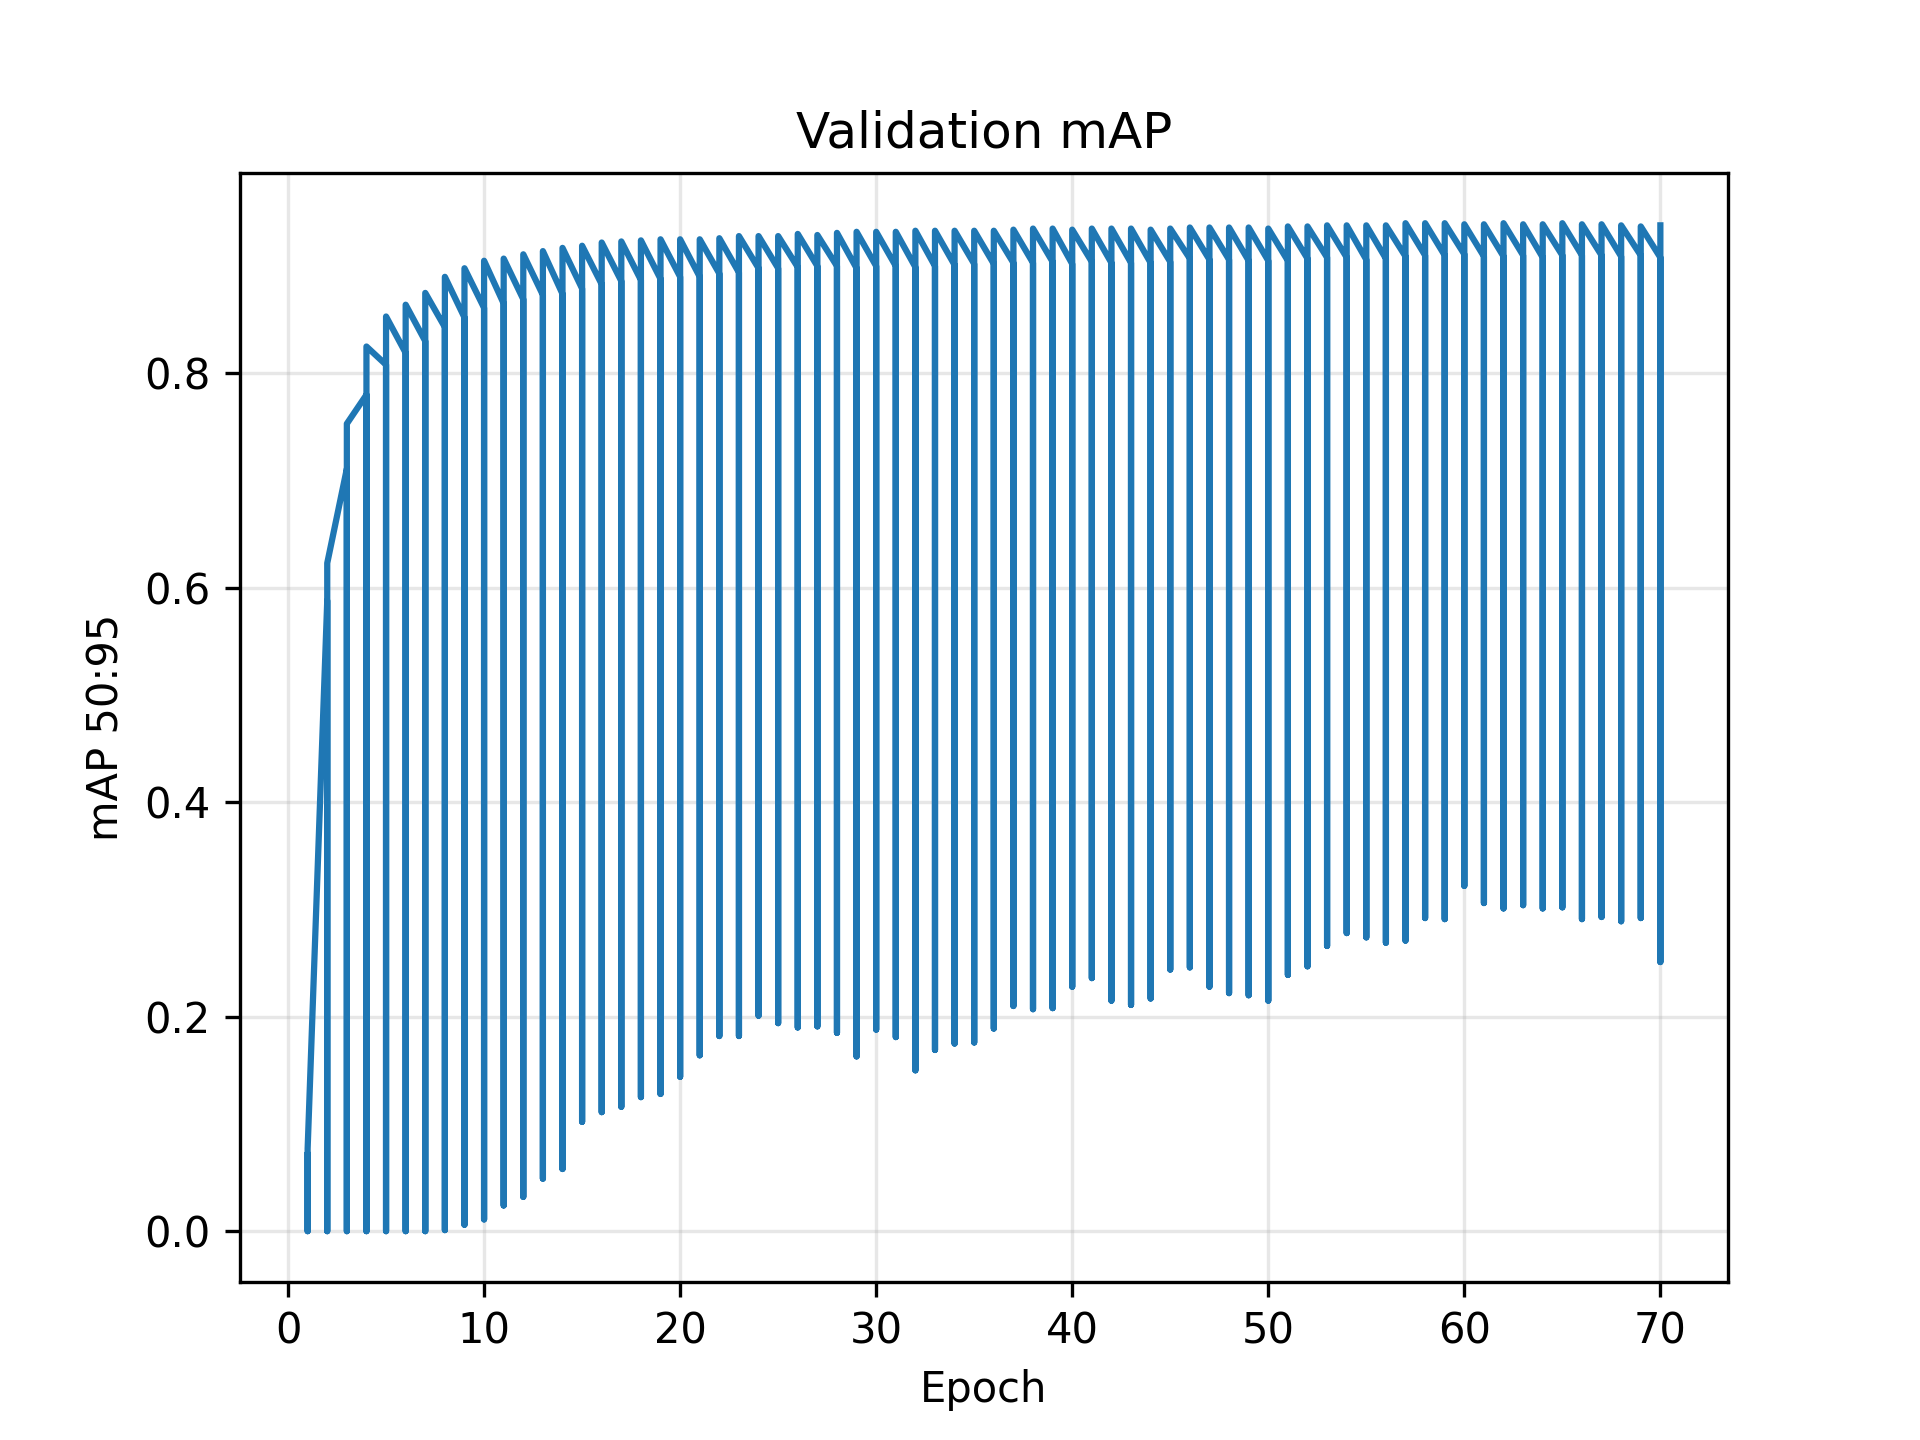
\includegraphics[width=\linewidth]{figures/images/chapter-11/qr-bar/v0/map_curve.png}
\caption{Validation mAP}
\end{subfigure}

\vspace{0.4cm}

\begin{subfigure}{0.50\textwidth}
\centering
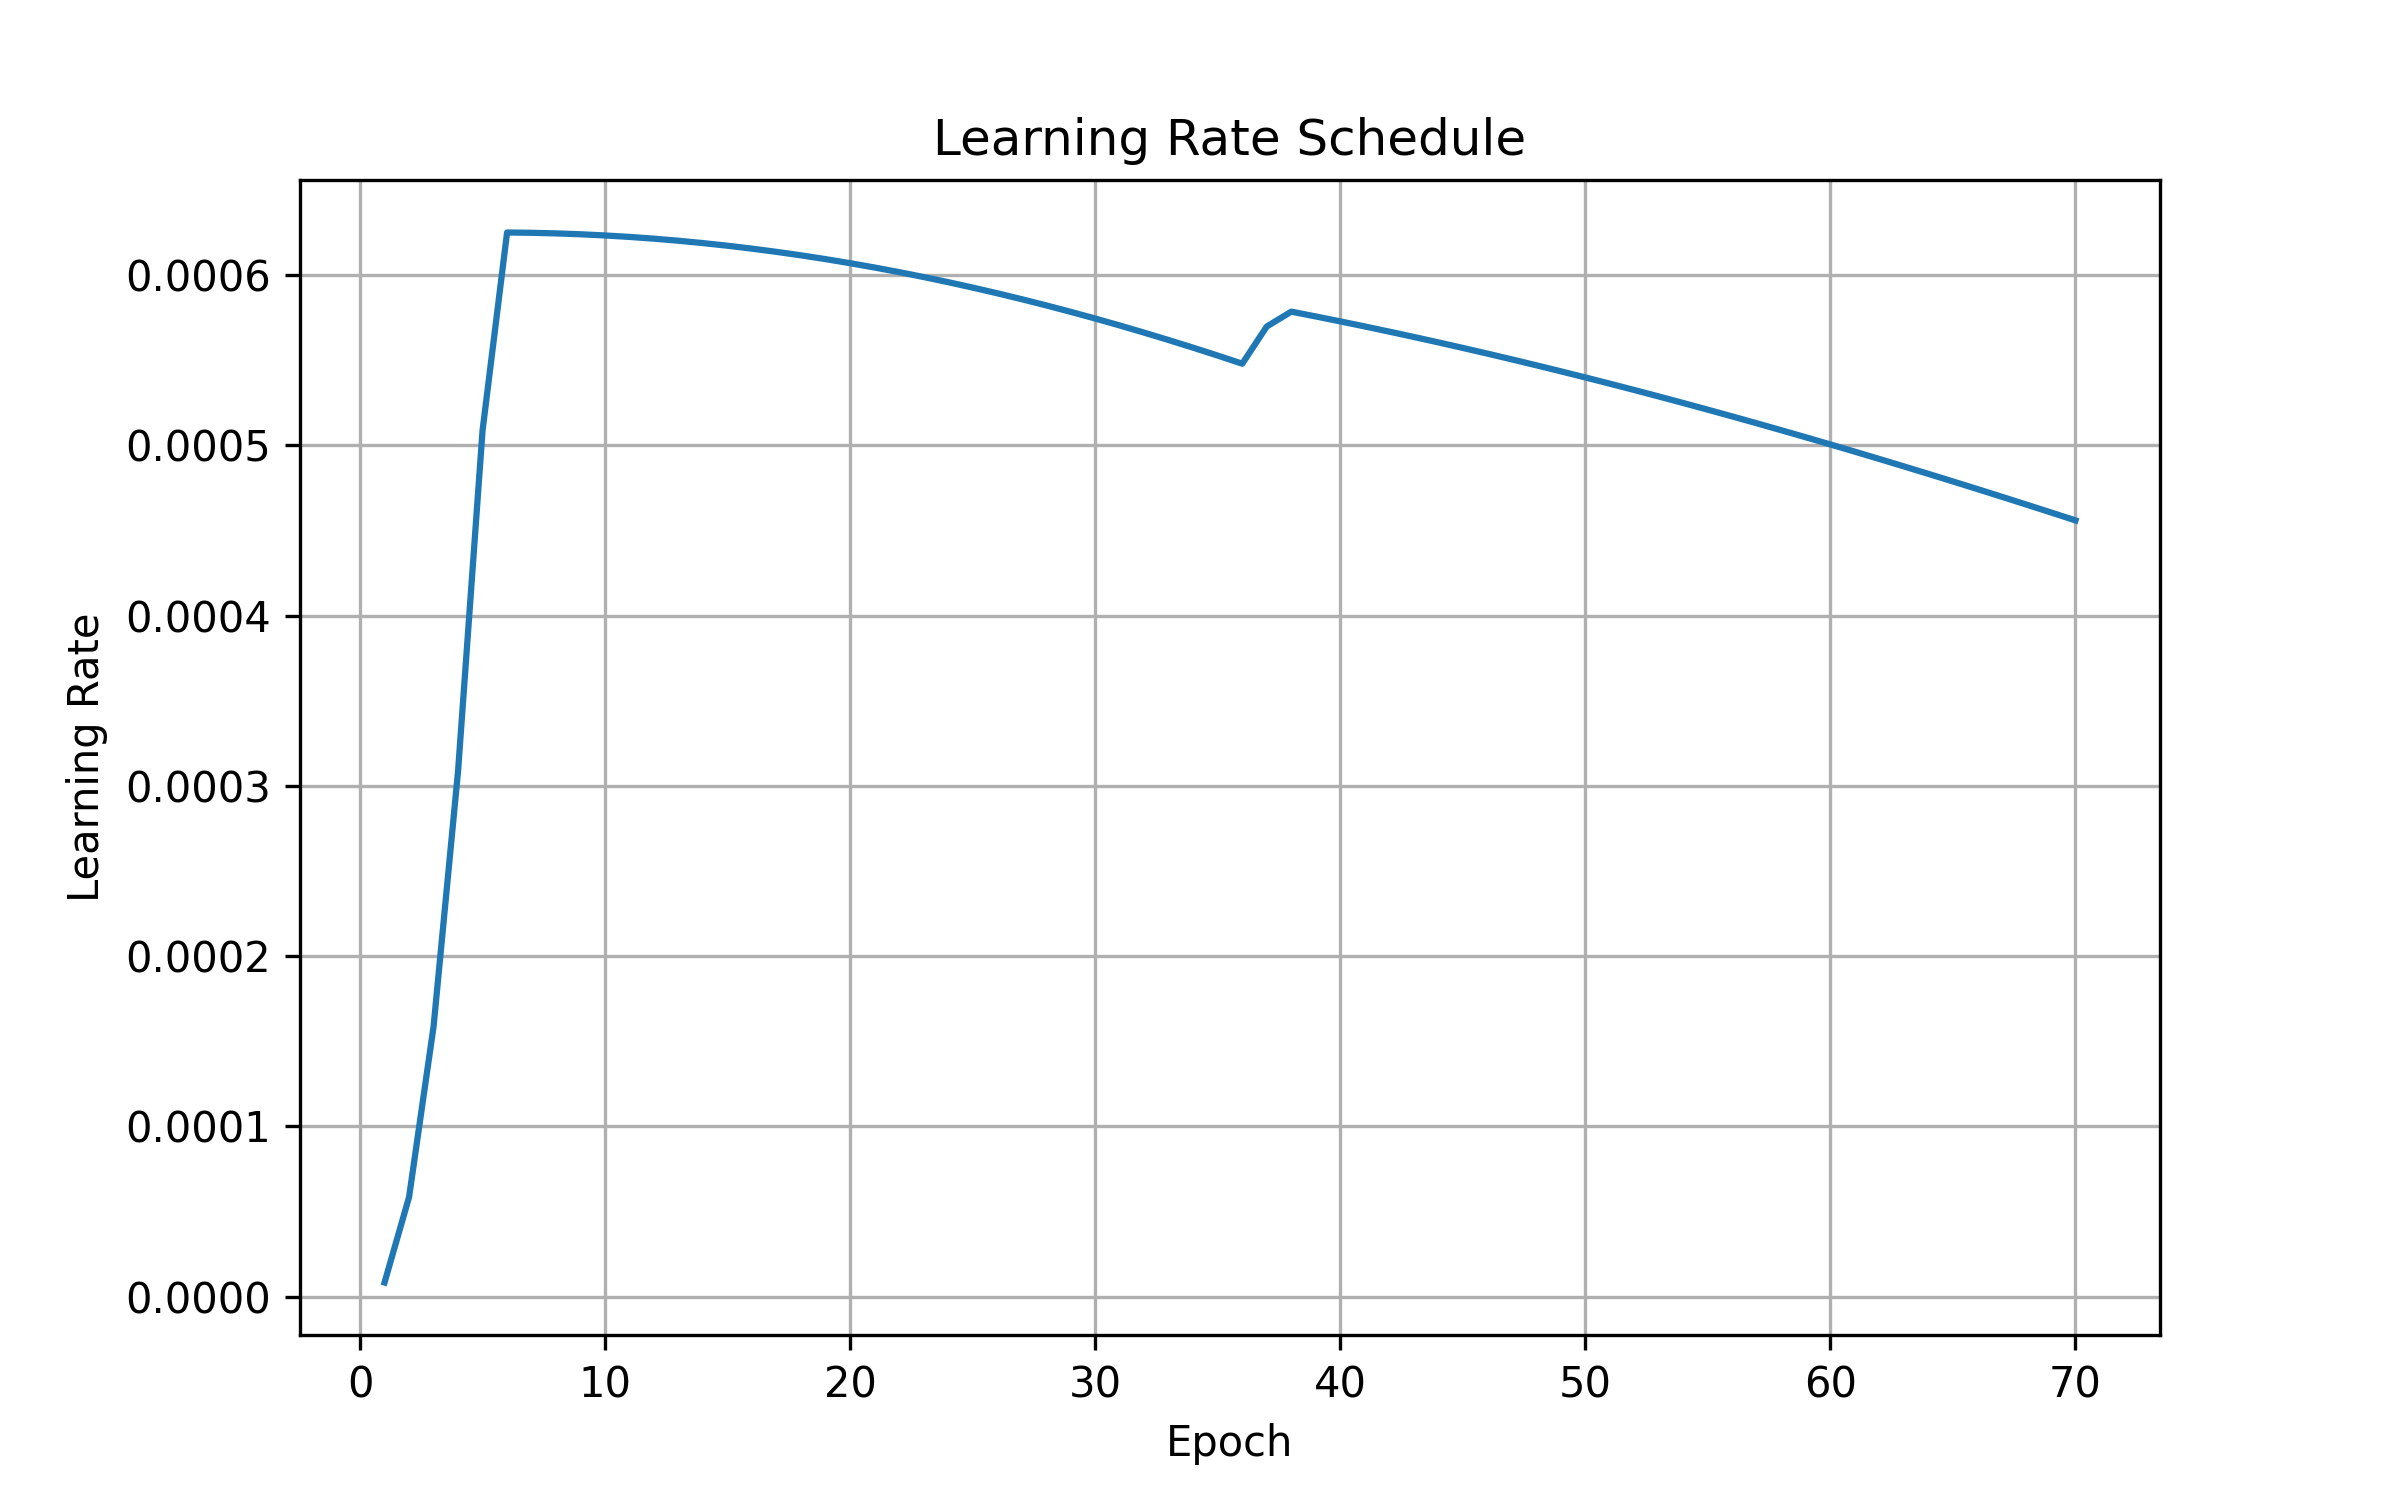
\includegraphics[width=\linewidth]{figures/images/chapter-11/qr-bar/v0/lr_curve.png}
\caption{Learning rate schedule}
\end{subfigure}

\caption{Training behaviour of the final barcode detection model.}
\label{fig:bc_training}
\end{figure}

The training loss decreases rapidly during the initial epochs and gradually
stabilizes, indicating successful convergence of the model.

The validation mAP increases quickly and stabilizes at a high level, showing
that the model generalizes well to unseen data.



\subsection{Precision--Recall Analysis}

\begin{figure}[H]
\centering
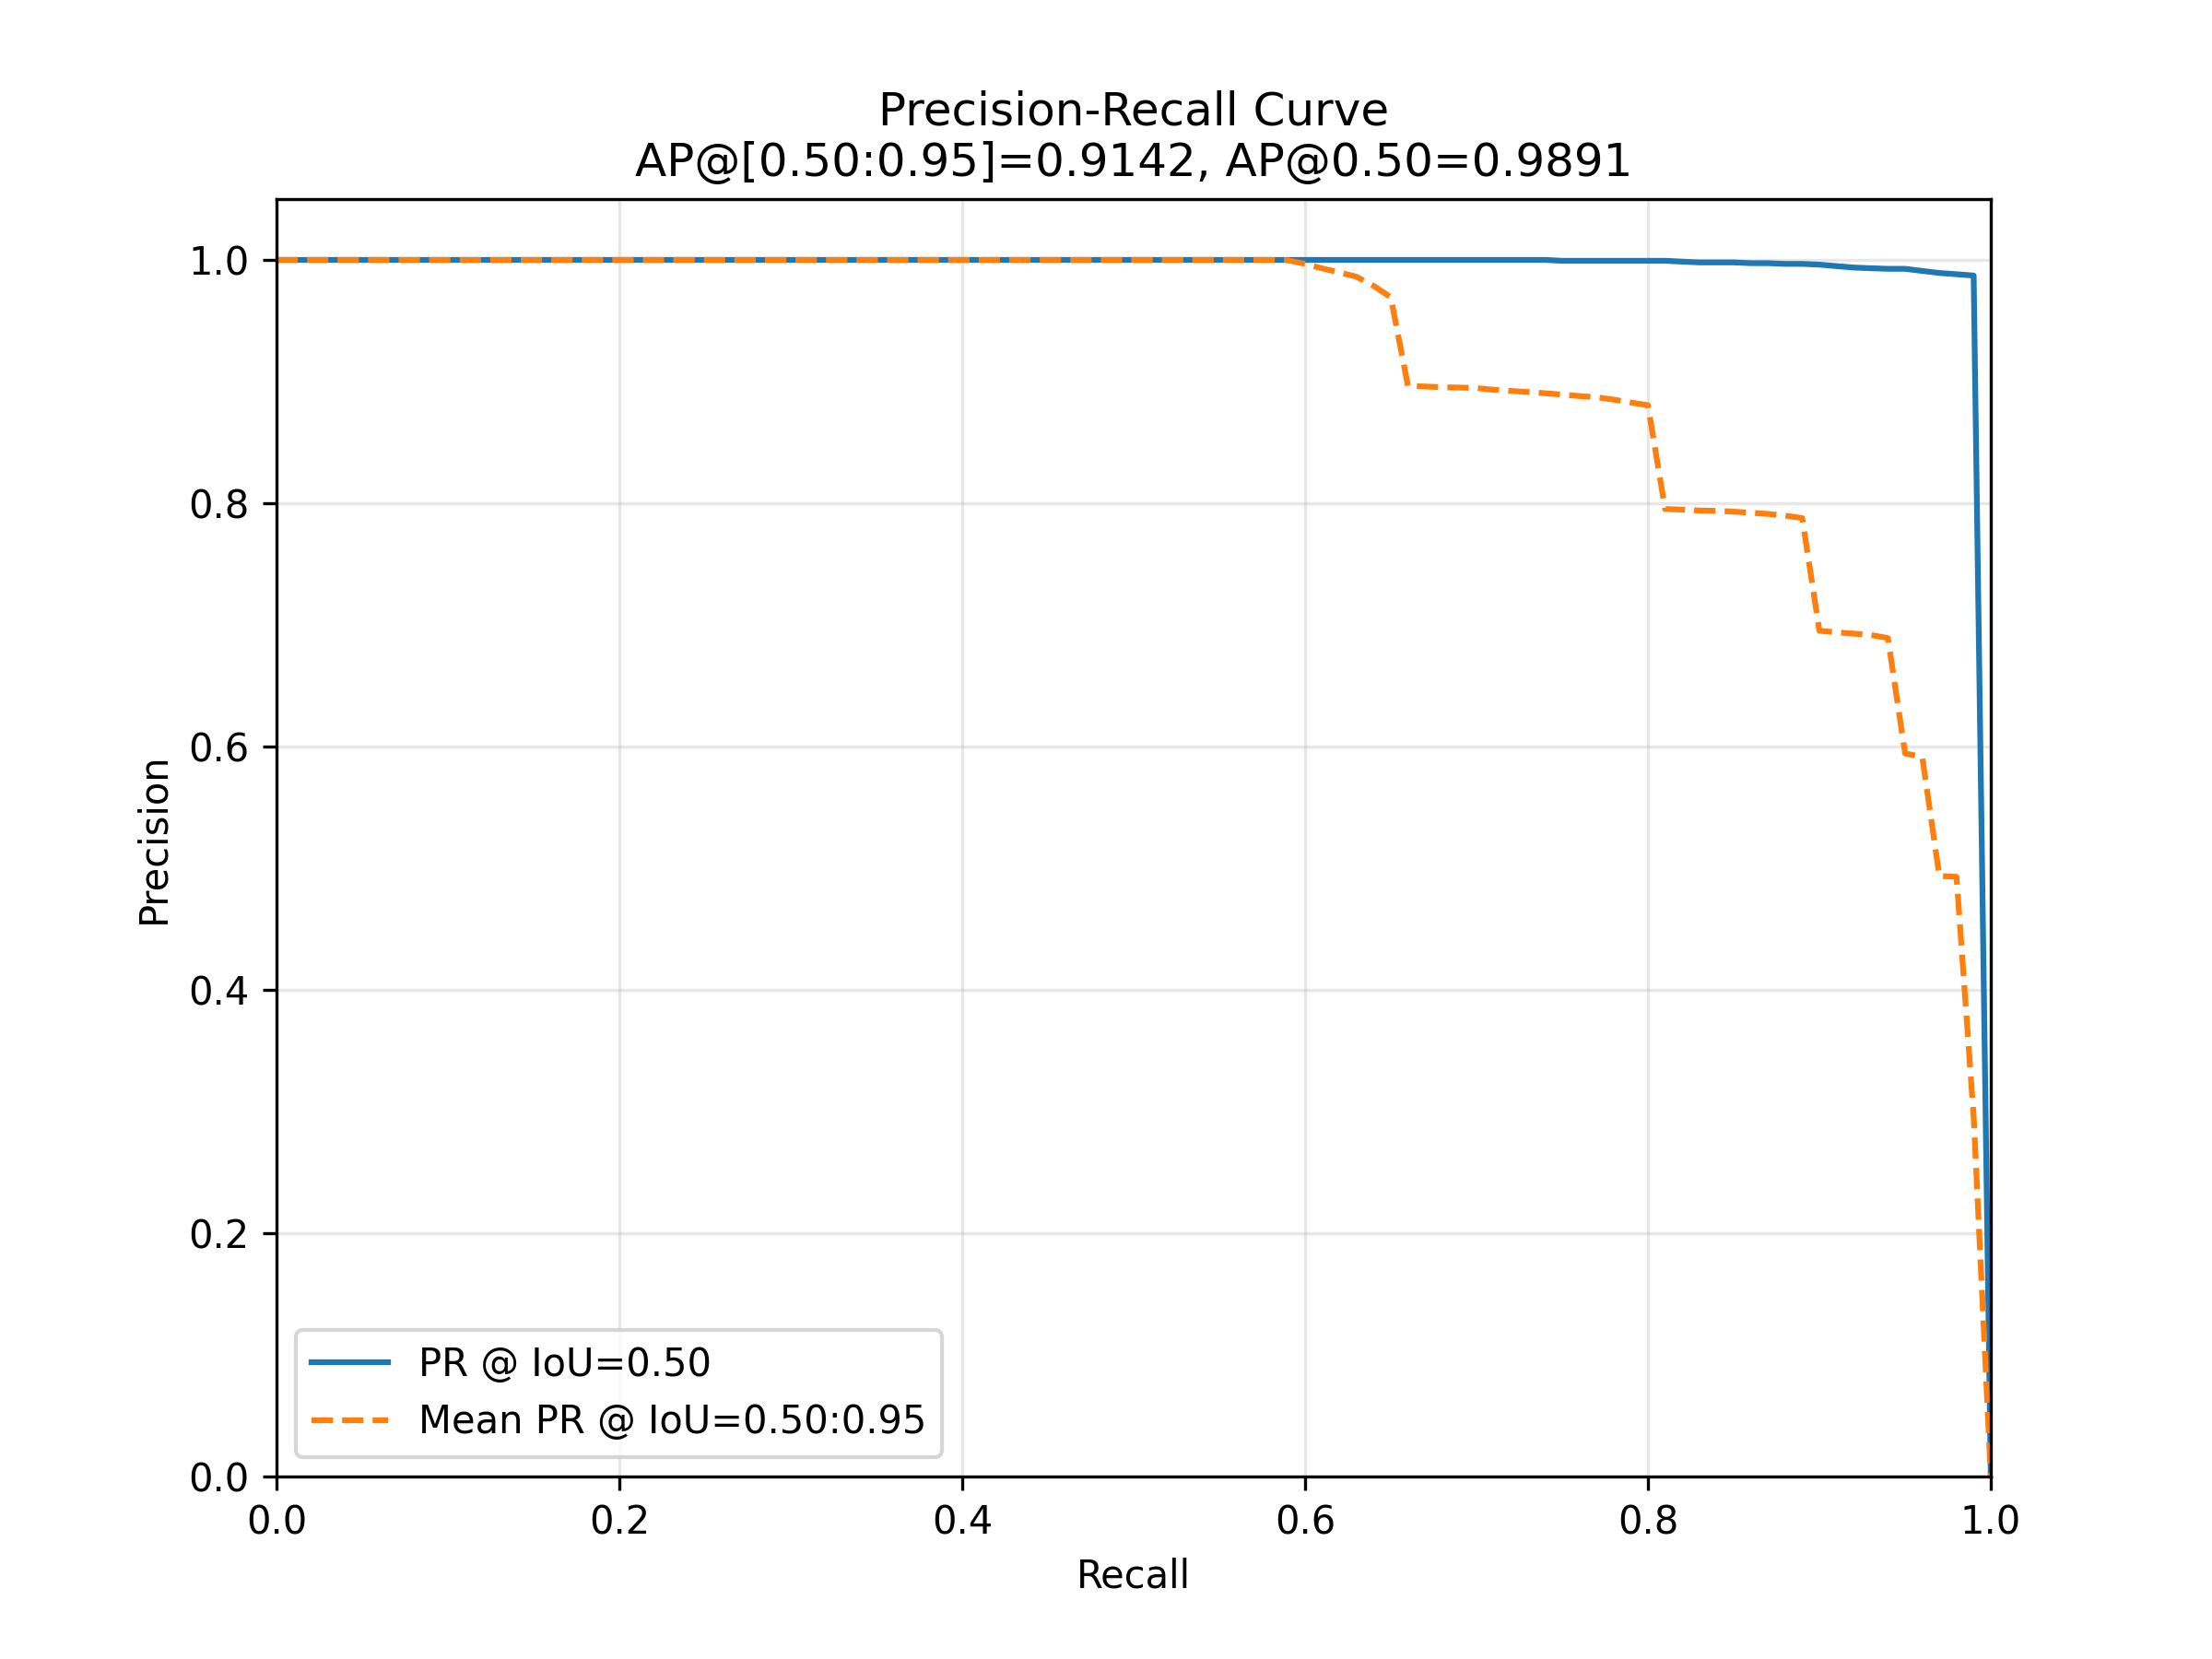
\includegraphics[width=10cm]{figures/images/chapter-11/qr-bar/v0/pr_curve.png}
\caption{Precision--recall curve for the barcode detection model.}
\label{fig:bc_pr_curve}
\end{figure}

The model achieves a high Average Precision, with
$AP@0.50 = 0.989$ and $AP@0.50:0.95 \approx 0.91$,
indicating strong detection performance across different IoU thresholds.




\subsection{Confusion Matrix Analysis}

\begin{figure}[H]
\centering
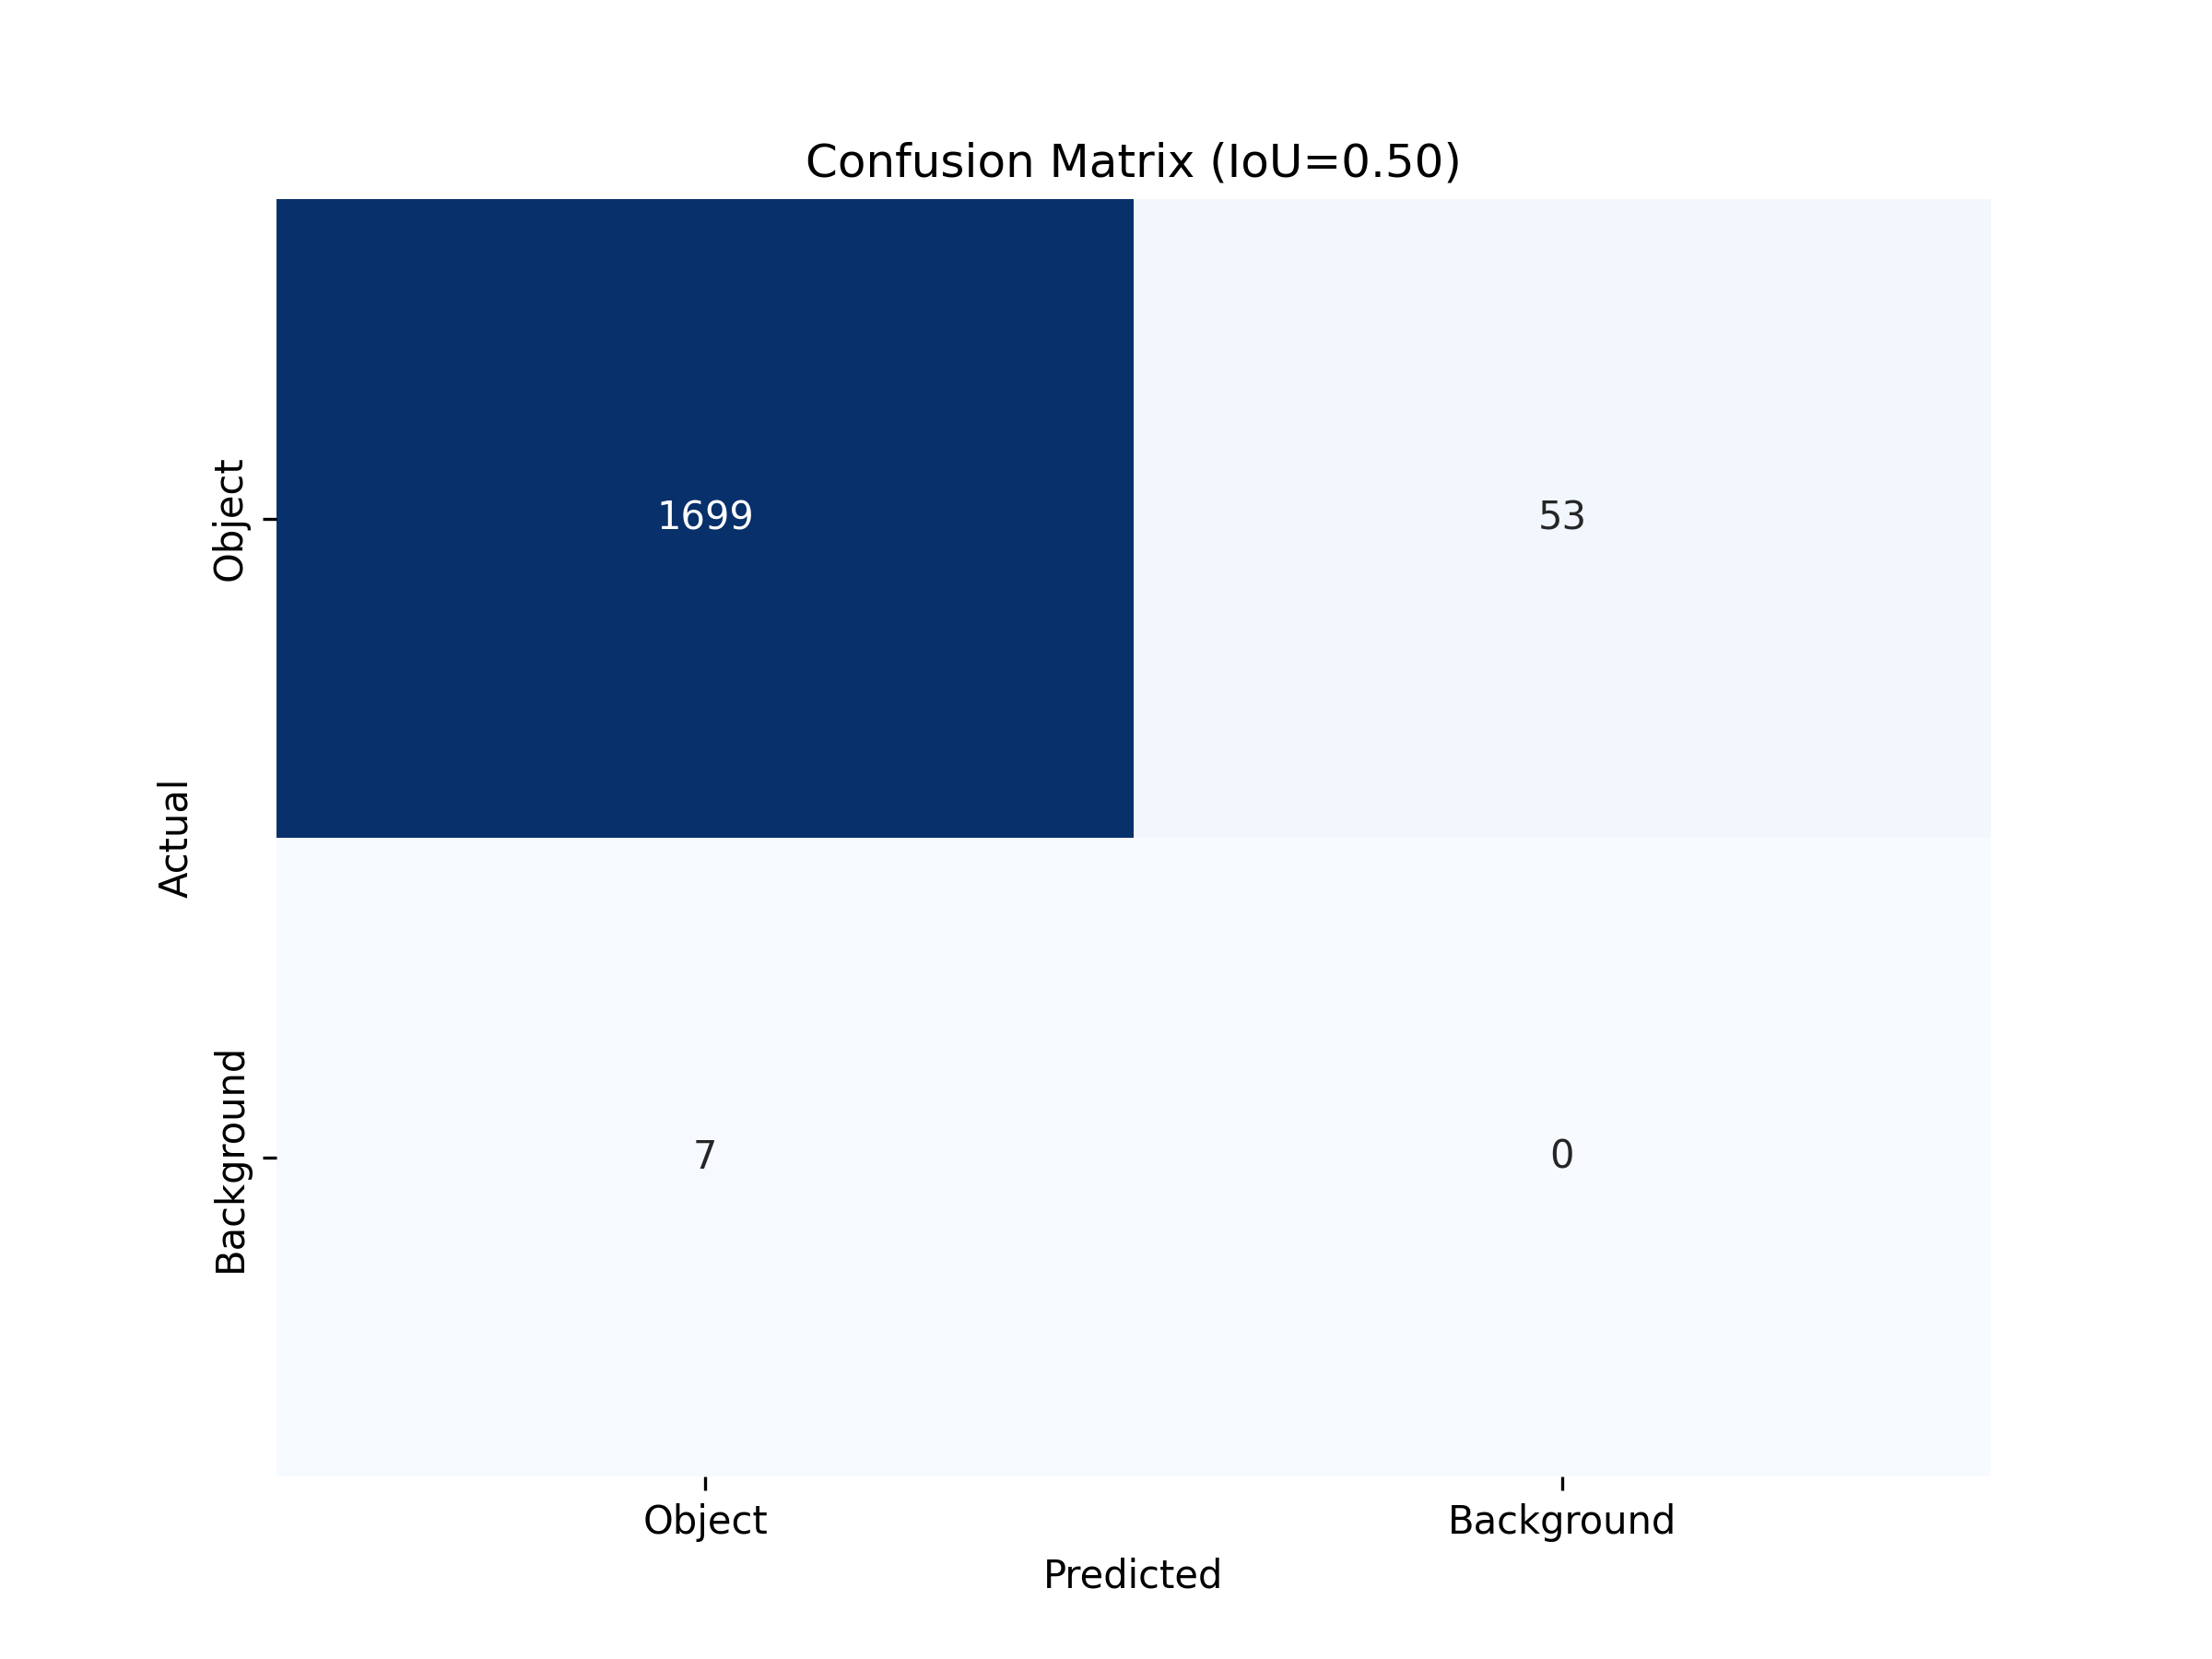
\includegraphics[width=12cm]{figures/images/chapter-11/qr-bar/v0/confusion_matrix_0.3.png}
\caption{Confusion matrix for the barcode detection model.}
\label{fig:bc_confusion_matrix}
\end{figure}

The model correctly detected 1699 barcodes, produced 53 false positives,
and missed 7 barcodes.

\begin{align*}
Precision &= \frac{1699}{1699 + 53} \approx 0.9697 \\
Recall &= \frac{1699}{1699 + 7} \approx 0.9959 \\
F1 &= 0.983
\end{align*}

\subsection{Summary}

The final barcode detection model achieved strong performance on the unseen
test set. At a confidence threshold of 0.3, the model obtained a precision of
96.97\%, a recall of 99.59\%, and an F1-score of 0.983.

The high recall indicates that the model missed very few barcodes, while the
high precision shows that most predicted detections were correct. Combined with
the high Average Precision values, these results indicate that the barcode
detector is suitable for use in the proposed system.






% ------------------------------------------------------------------------


\section{License Plate Detection}
\label{app:license_plate_results}

This section documents the detailed training and evaluation results for the
custom-trained license plate detection models. The model was trained using the
same YOLOX-based training pipeline as the barcode detection model. Therefore,
this section focuses on the supporting results used to evaluate and compare the
license plate detector configurations.


\subsection{Training Setup}

\begin{table}[H]
\centering
\begin{tabular}{l l p{5.0cm}}
\toprule
\textbf{Dataset} & \textbf{Source} & \textbf{Description} \\
\midrule
License Plate Detection Dataset
& Kaggle \cite{lp_dataset_1} 
& Dataset containing annotated license plate images from real-world environments, designed for object detection tasks \\

Large License Plate Detection Dataset
& Kaggle \cite{lp_dataset_2} 
& Large-scale dataset with diverse license plate instances captured under varying lighting and environmental conditions \\

\midrule
\textbf{Total} & 38025 & Combined into a unified dataset for training and evaluation \\
\bottomrule
\end{tabular}
\caption{Overview of datasets used for training the license plate detection model.}
\label{tab:licenseplate_datasets}
\end{table}



The dataset was divided into approximately 85\% training, 10\% validation, and
5\% testing. After excluding three label files, the dataset consisted of 36,959 images. This split was chosen to provide a large number of training
samples while still reserving separate validation and test sets for monitoring
training performance and evaluating the final model on unseen data. Both models
used the same training, validation, and test split.


\begin{table}[H]
\centering

\begin{minipage}[t]{0.43\textwidth}
\centering
\caption{Training Configuration for Model V0}
\label{tab:lp_training_config_v0}
\scriptsize
\renewcommand{\arraystretch}{1.05}
\begin{tabular}{>{\raggedright\arraybackslash}p{0.52\linewidth}
                >{\raggedright\arraybackslash}p{0.38\linewidth}}
\toprule
\textbf{Parameter} & \textbf{Value} \\
\midrule
Architecture & YOLOX-S \\
Input Resolution & $640 \times 640$ \\
Batch Size & 16 \\
Max Epochs & 200 \\
No-Aug. Epochs & 15 \\
\midrule
\textit{Optimization} & \\
Base Learning Rate & 0.01 / 64 \\
Warmup Epochs & 5 \\
Min LR Ratio & 0.05 \\
Optimizer & SGD \\
\midrule
\textit{Augmentation (Offline)} & \\
Mosaic Images & 0.8 (0.3--1.8) \\
Color / Flip & 0.5 / 0.5 \\
Rotation / Shift / Shear & 5.0 / 0.05 / 1.0 \\
Random Image Size & (10, 20) \\
\midrule
\textit{Hardware} & \\
GPU Model & RTX 4080 \\
\bottomrule
\end{tabular}
\end{minipage}
\hfill
\begin{minipage}[t]{0.43\textwidth}
\centering
\caption{Training Configuration for Model V1}
\label{tab:lp_training_config_v1}
\scriptsize
\renewcommand{\arraystretch}{1.05}
\begin{tabular}{>{\raggedright\arraybackslash}p{0.52\linewidth}
                >{\raggedright\arraybackslash}p{0.38\linewidth}}
\toprule
\textbf{Parameter} & \textbf{Value} \\
\midrule
Architecture & YOLOX-S \\
Input Resolution & $960 \times 960$ \\
Batch Size & 8 \\
Max Epochs & 200 \\
No-Aug. Epochs & 15 \\
\midrule
\textit{Optimization} & \\
Base Learning Rate & 0.01 / 64 \\
Warmup Epochs & 5 \\
Min LR Ratio & 0.05 \\
Optimizer & SGD \\
\midrule
\textit{Augmentation (Offline)} & \\
Mosaic Images & 0.8 (0.5--1.5) \\
Color / Flip & 0.5 / 0.5 \\
Rotation / Shift / Shear & 5.0 / 0.05 / 1.0 \\
Random Image Size & (14, 24) \\
\midrule
\textit{Hardware} & \\
GPU Model & RTX 4080 \\
\bottomrule
\end{tabular}
\end{minipage}

\end{table}

Tables~\ref{tab:lp_training_config_v0} and~\ref{tab:lp_training_config_v1}
summarize the training configurations for the two license plate detection
models. The main difference was the increased input resolution in v1, which
required a smaller batch size.



\subsection{Training Curves}


\begin{figure}[H]
\centering

\begin{subfigure}{0.50\textwidth}
\centering
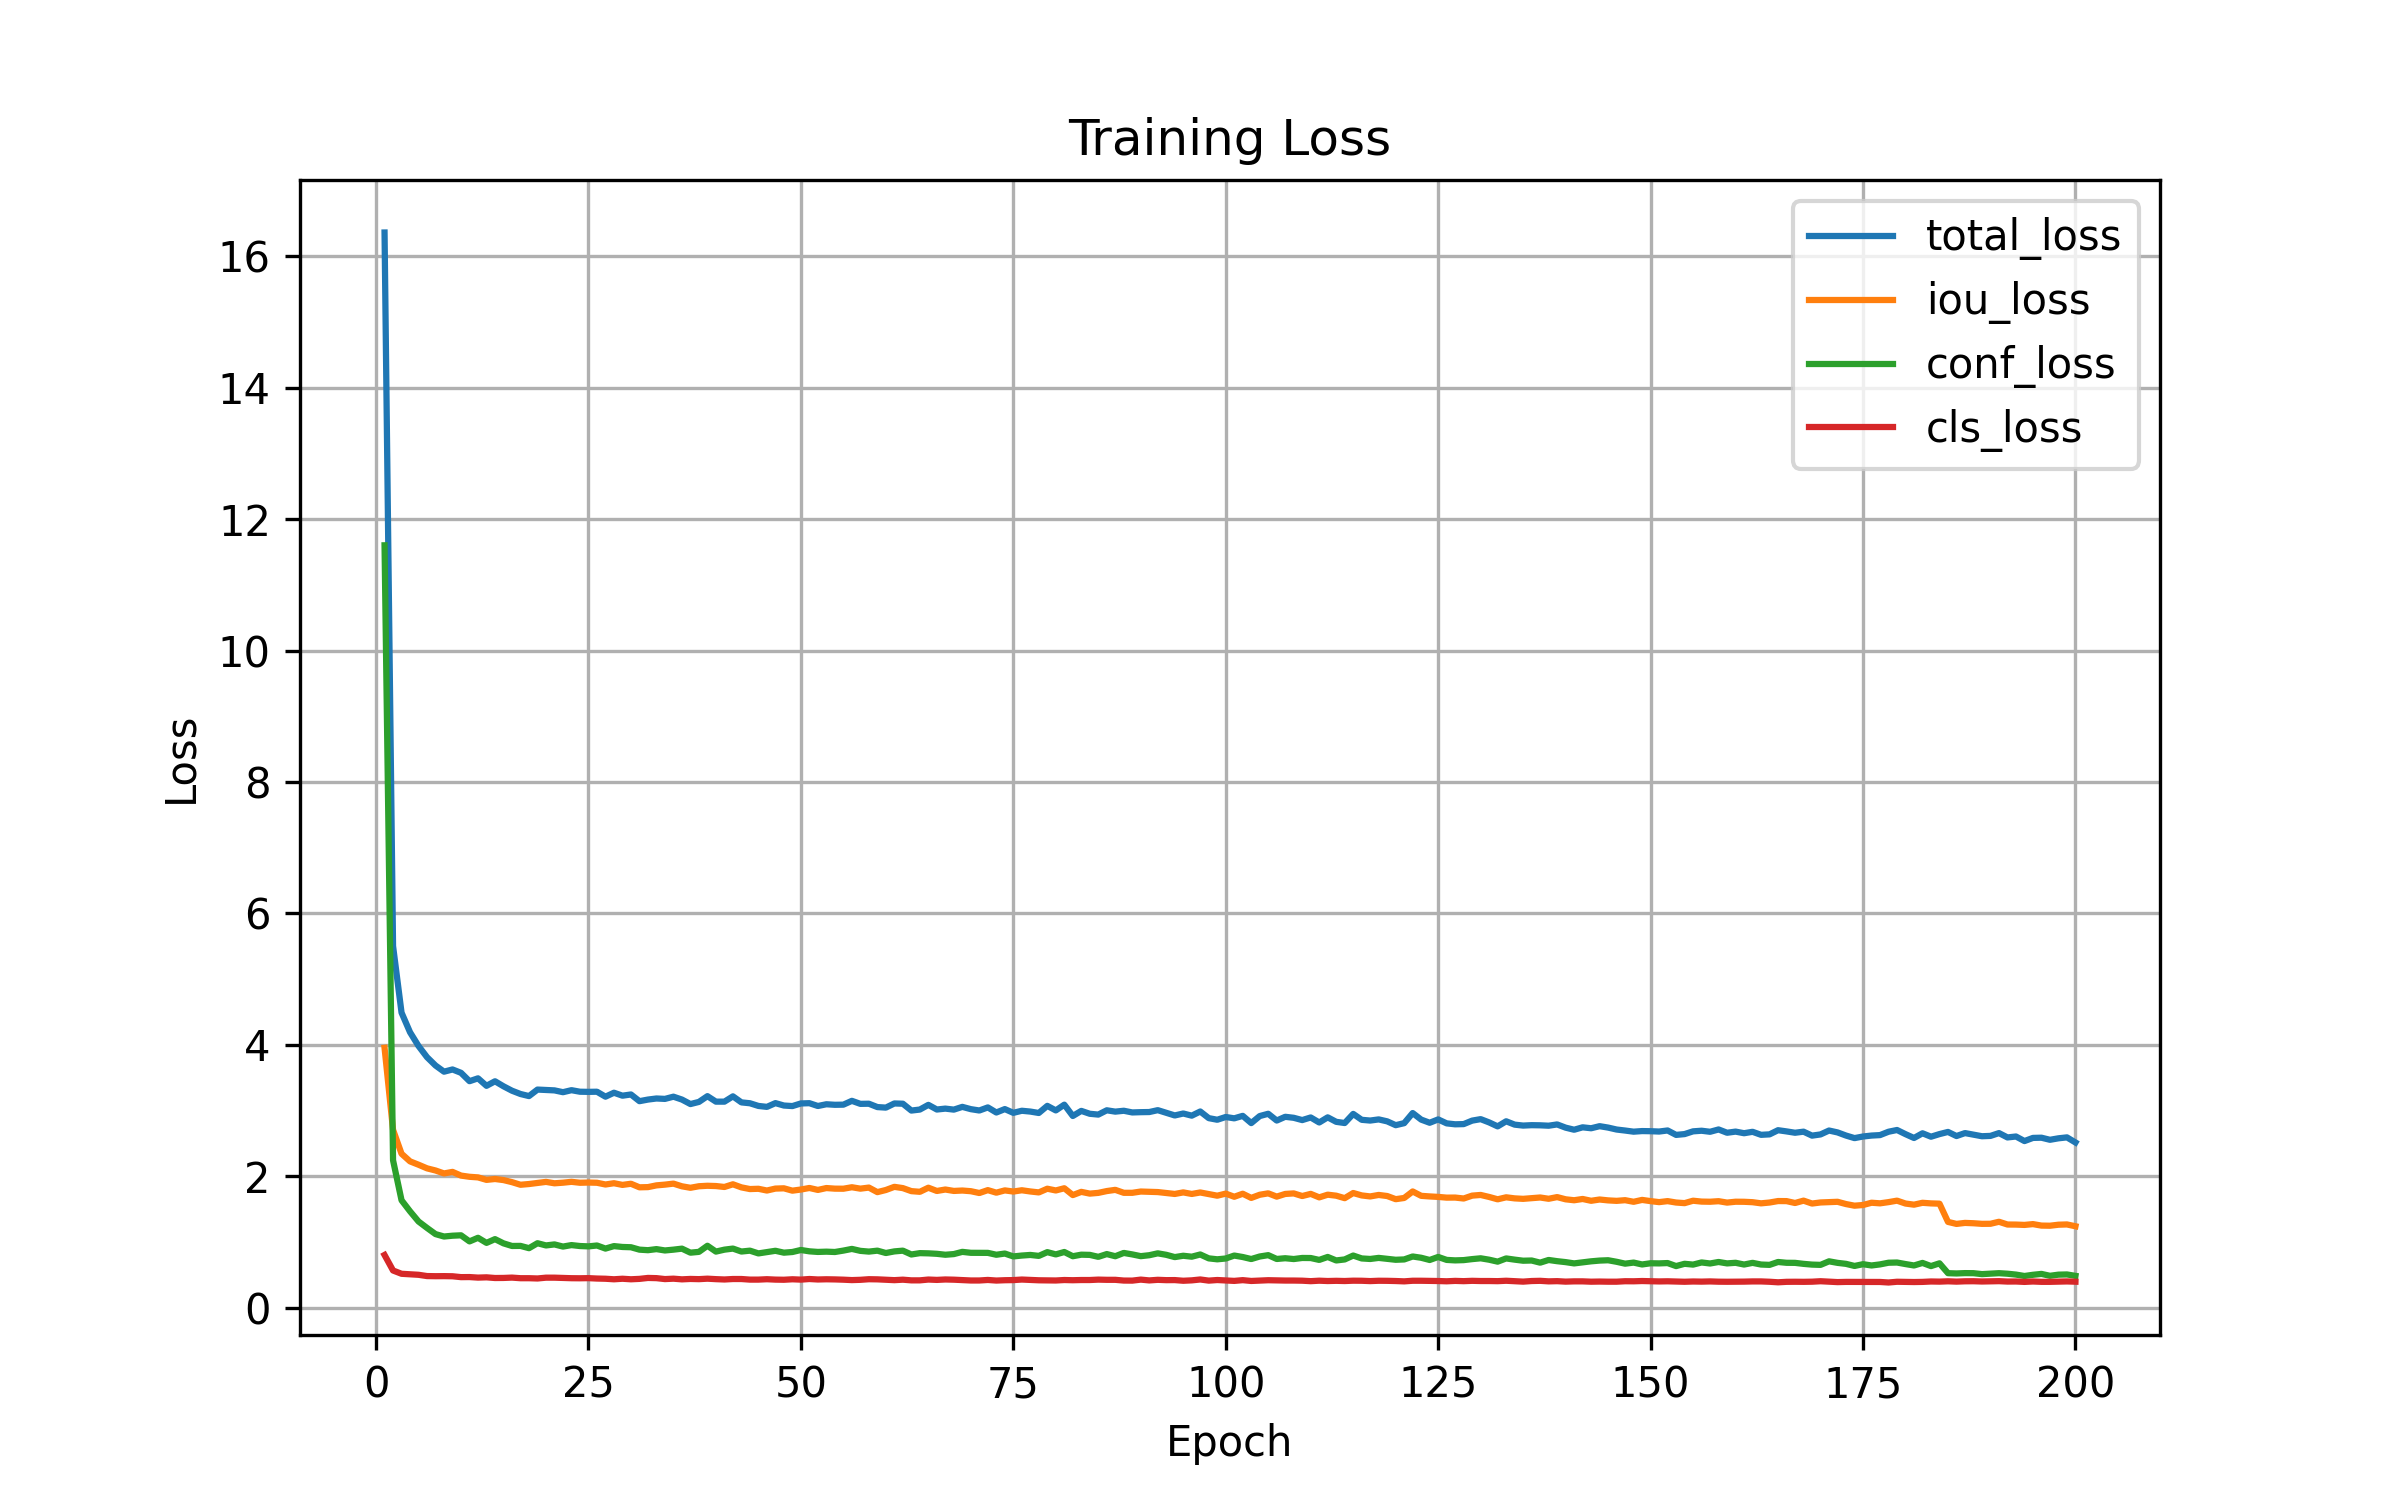
\includegraphics[width=\linewidth]{figures/images/chapter-11/licenseplate/v0/loss_curve.png}
\caption{Training loss}
\end{subfigure}
\hfill
\begin{subfigure}{0.48\textwidth}
\centering
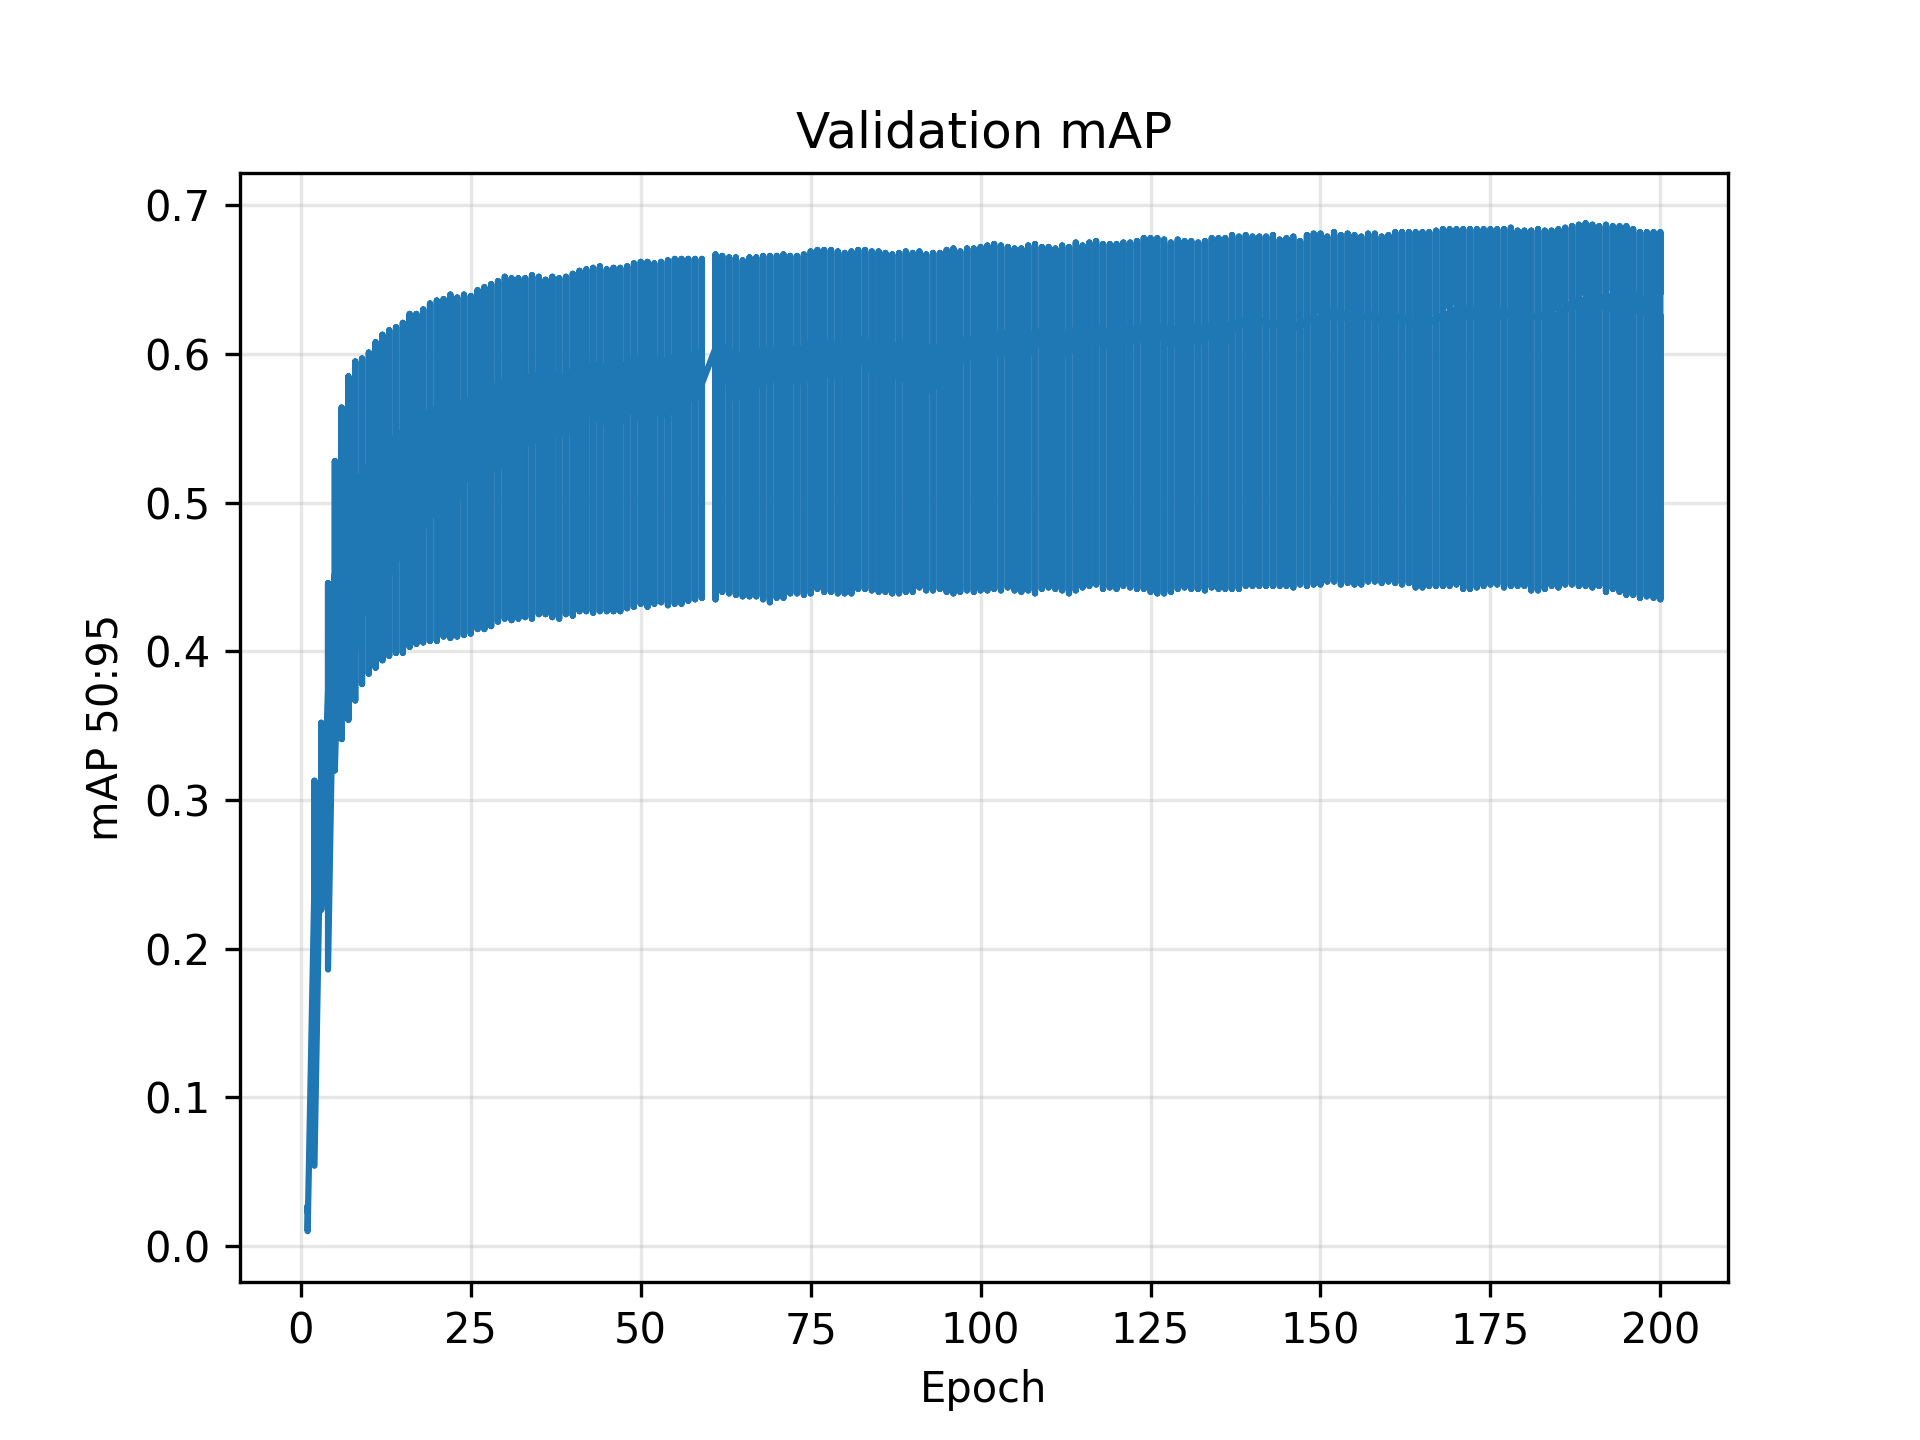
\includegraphics[width=\linewidth]{figures/images/chapter-11/licenseplate/v0/map_curve.png}
\caption{Validation mAP}
\end{subfigure}

\vspace{0.4cm}

\begin{subfigure}{0.50\textwidth}
\centering
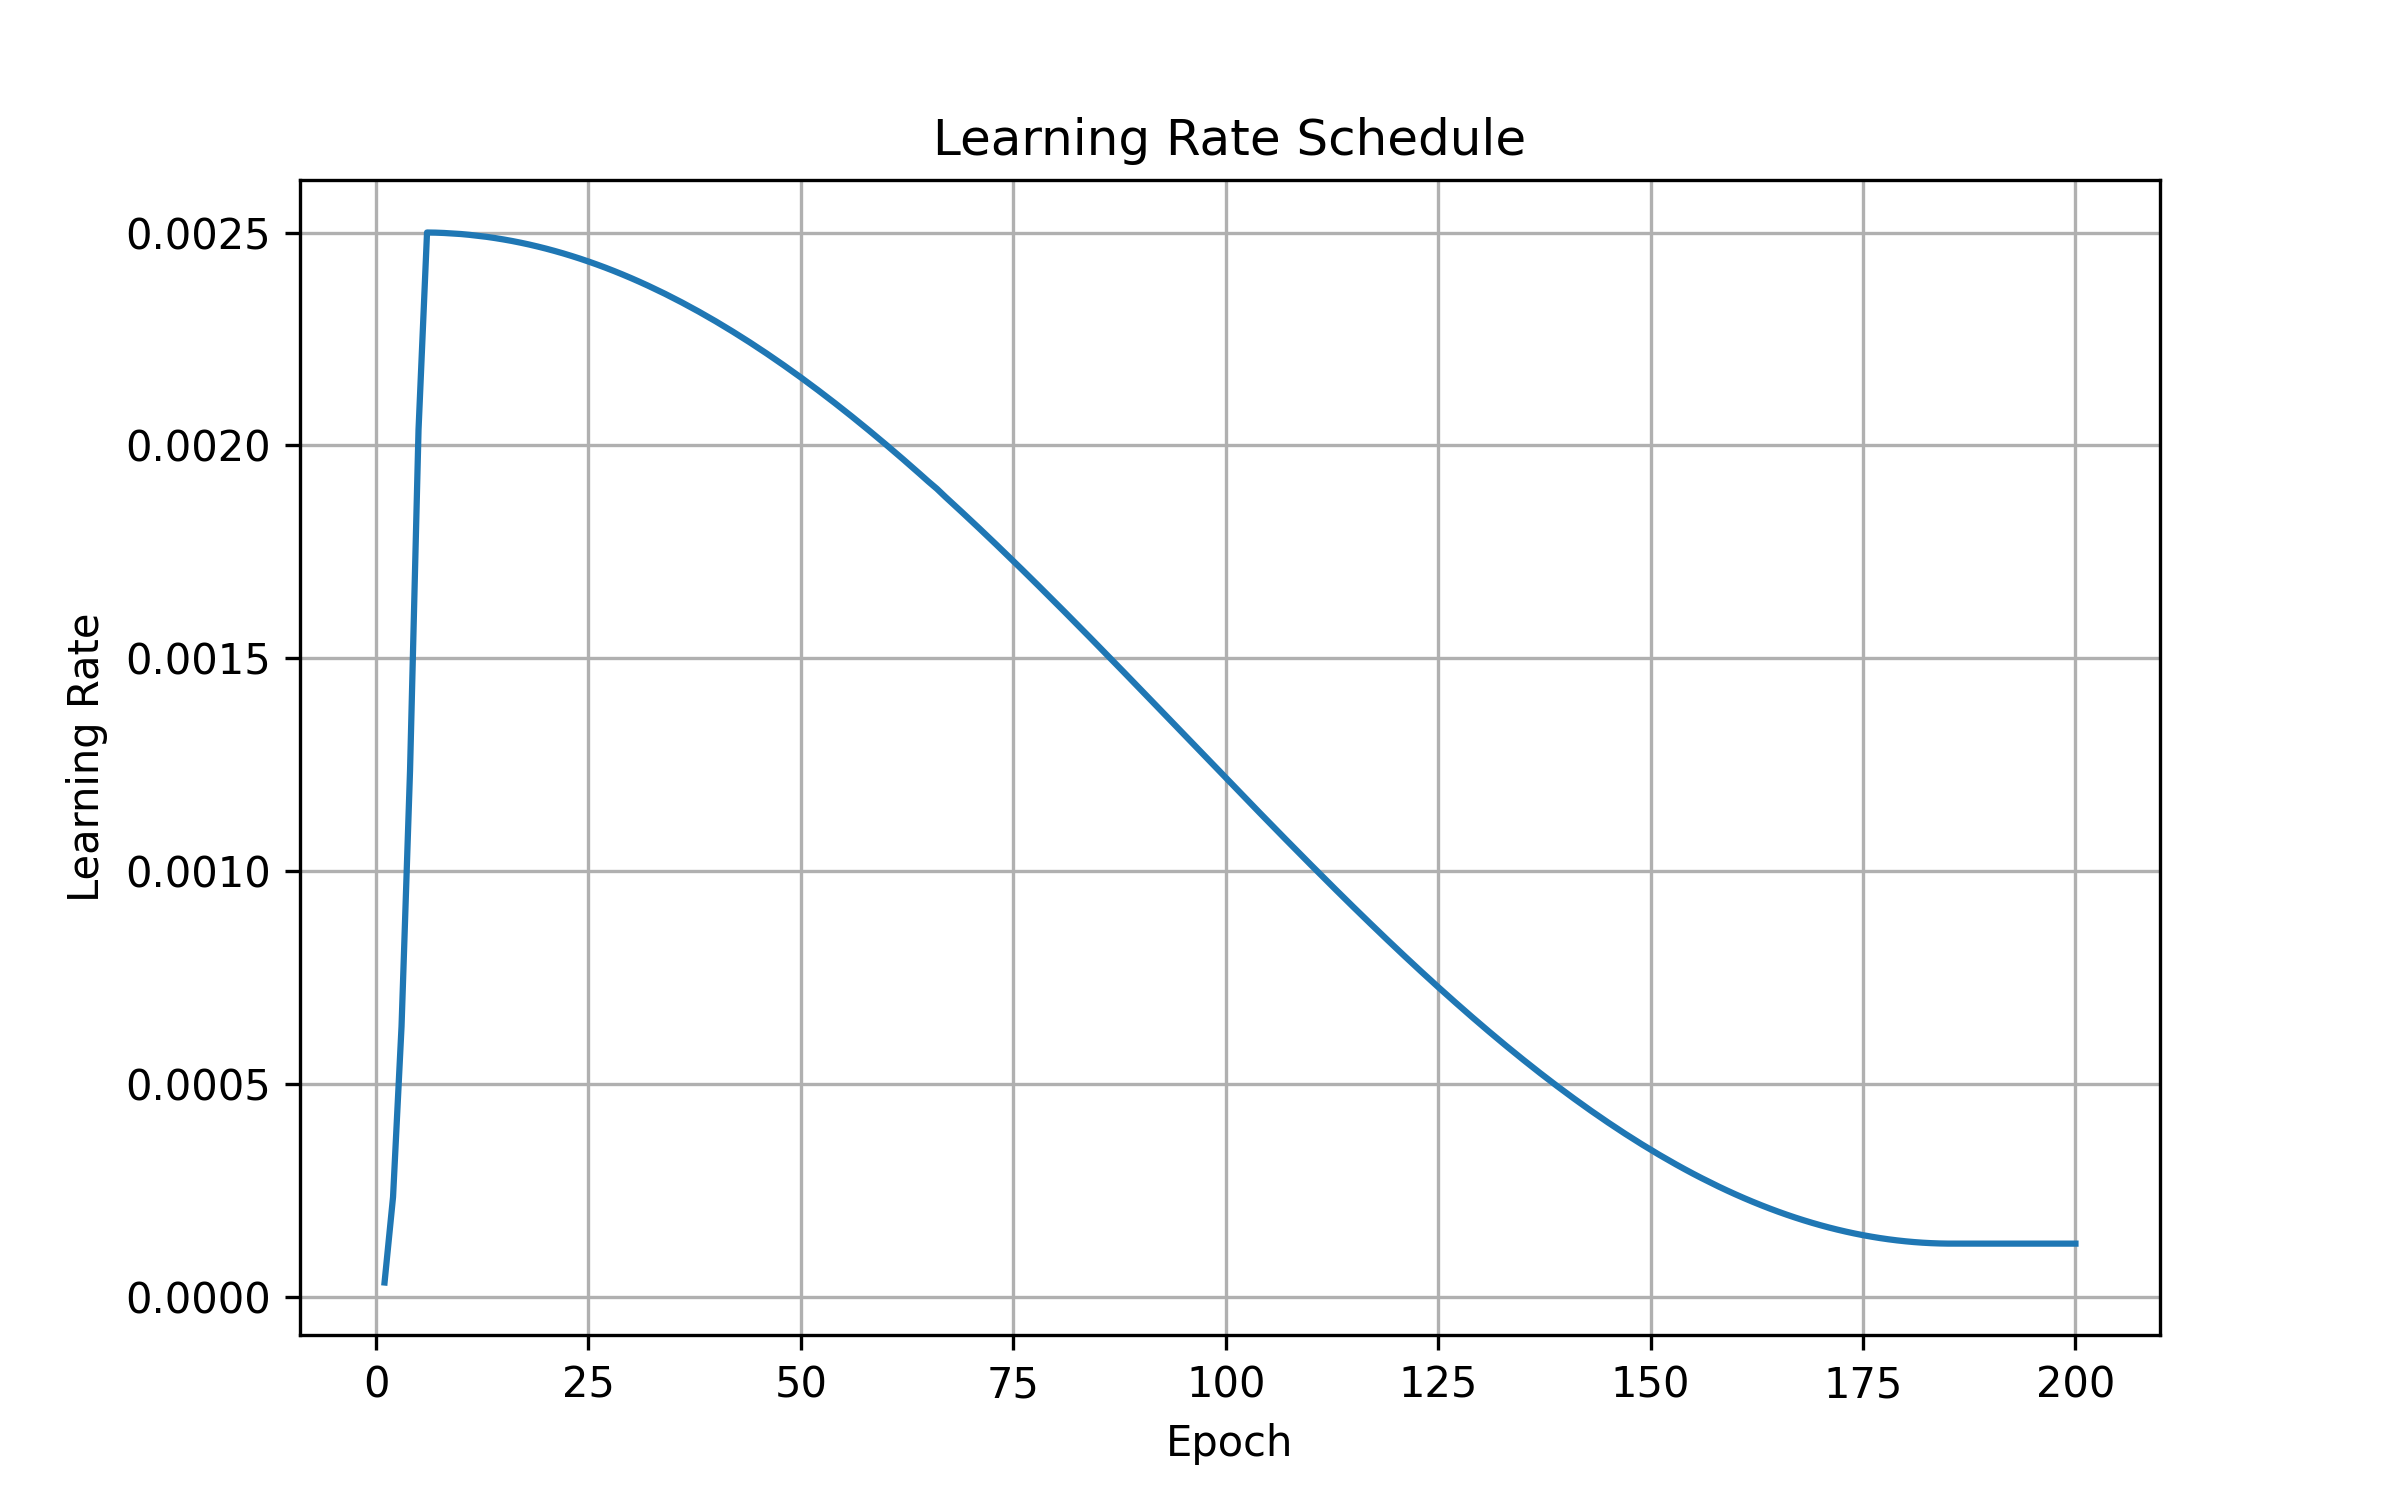
\includegraphics[width=\linewidth]{figures/images/chapter-11/licenseplate/v0/lr_curve.png}
\caption{Learning rate schedule}
\end{subfigure}

\caption{Training behaviour of model v0.}
\label{fig:lp_training_v0}

\end{figure}

\begin{figure}[H]
\centering

\begin{subfigure}{0.50\textwidth}
\centering
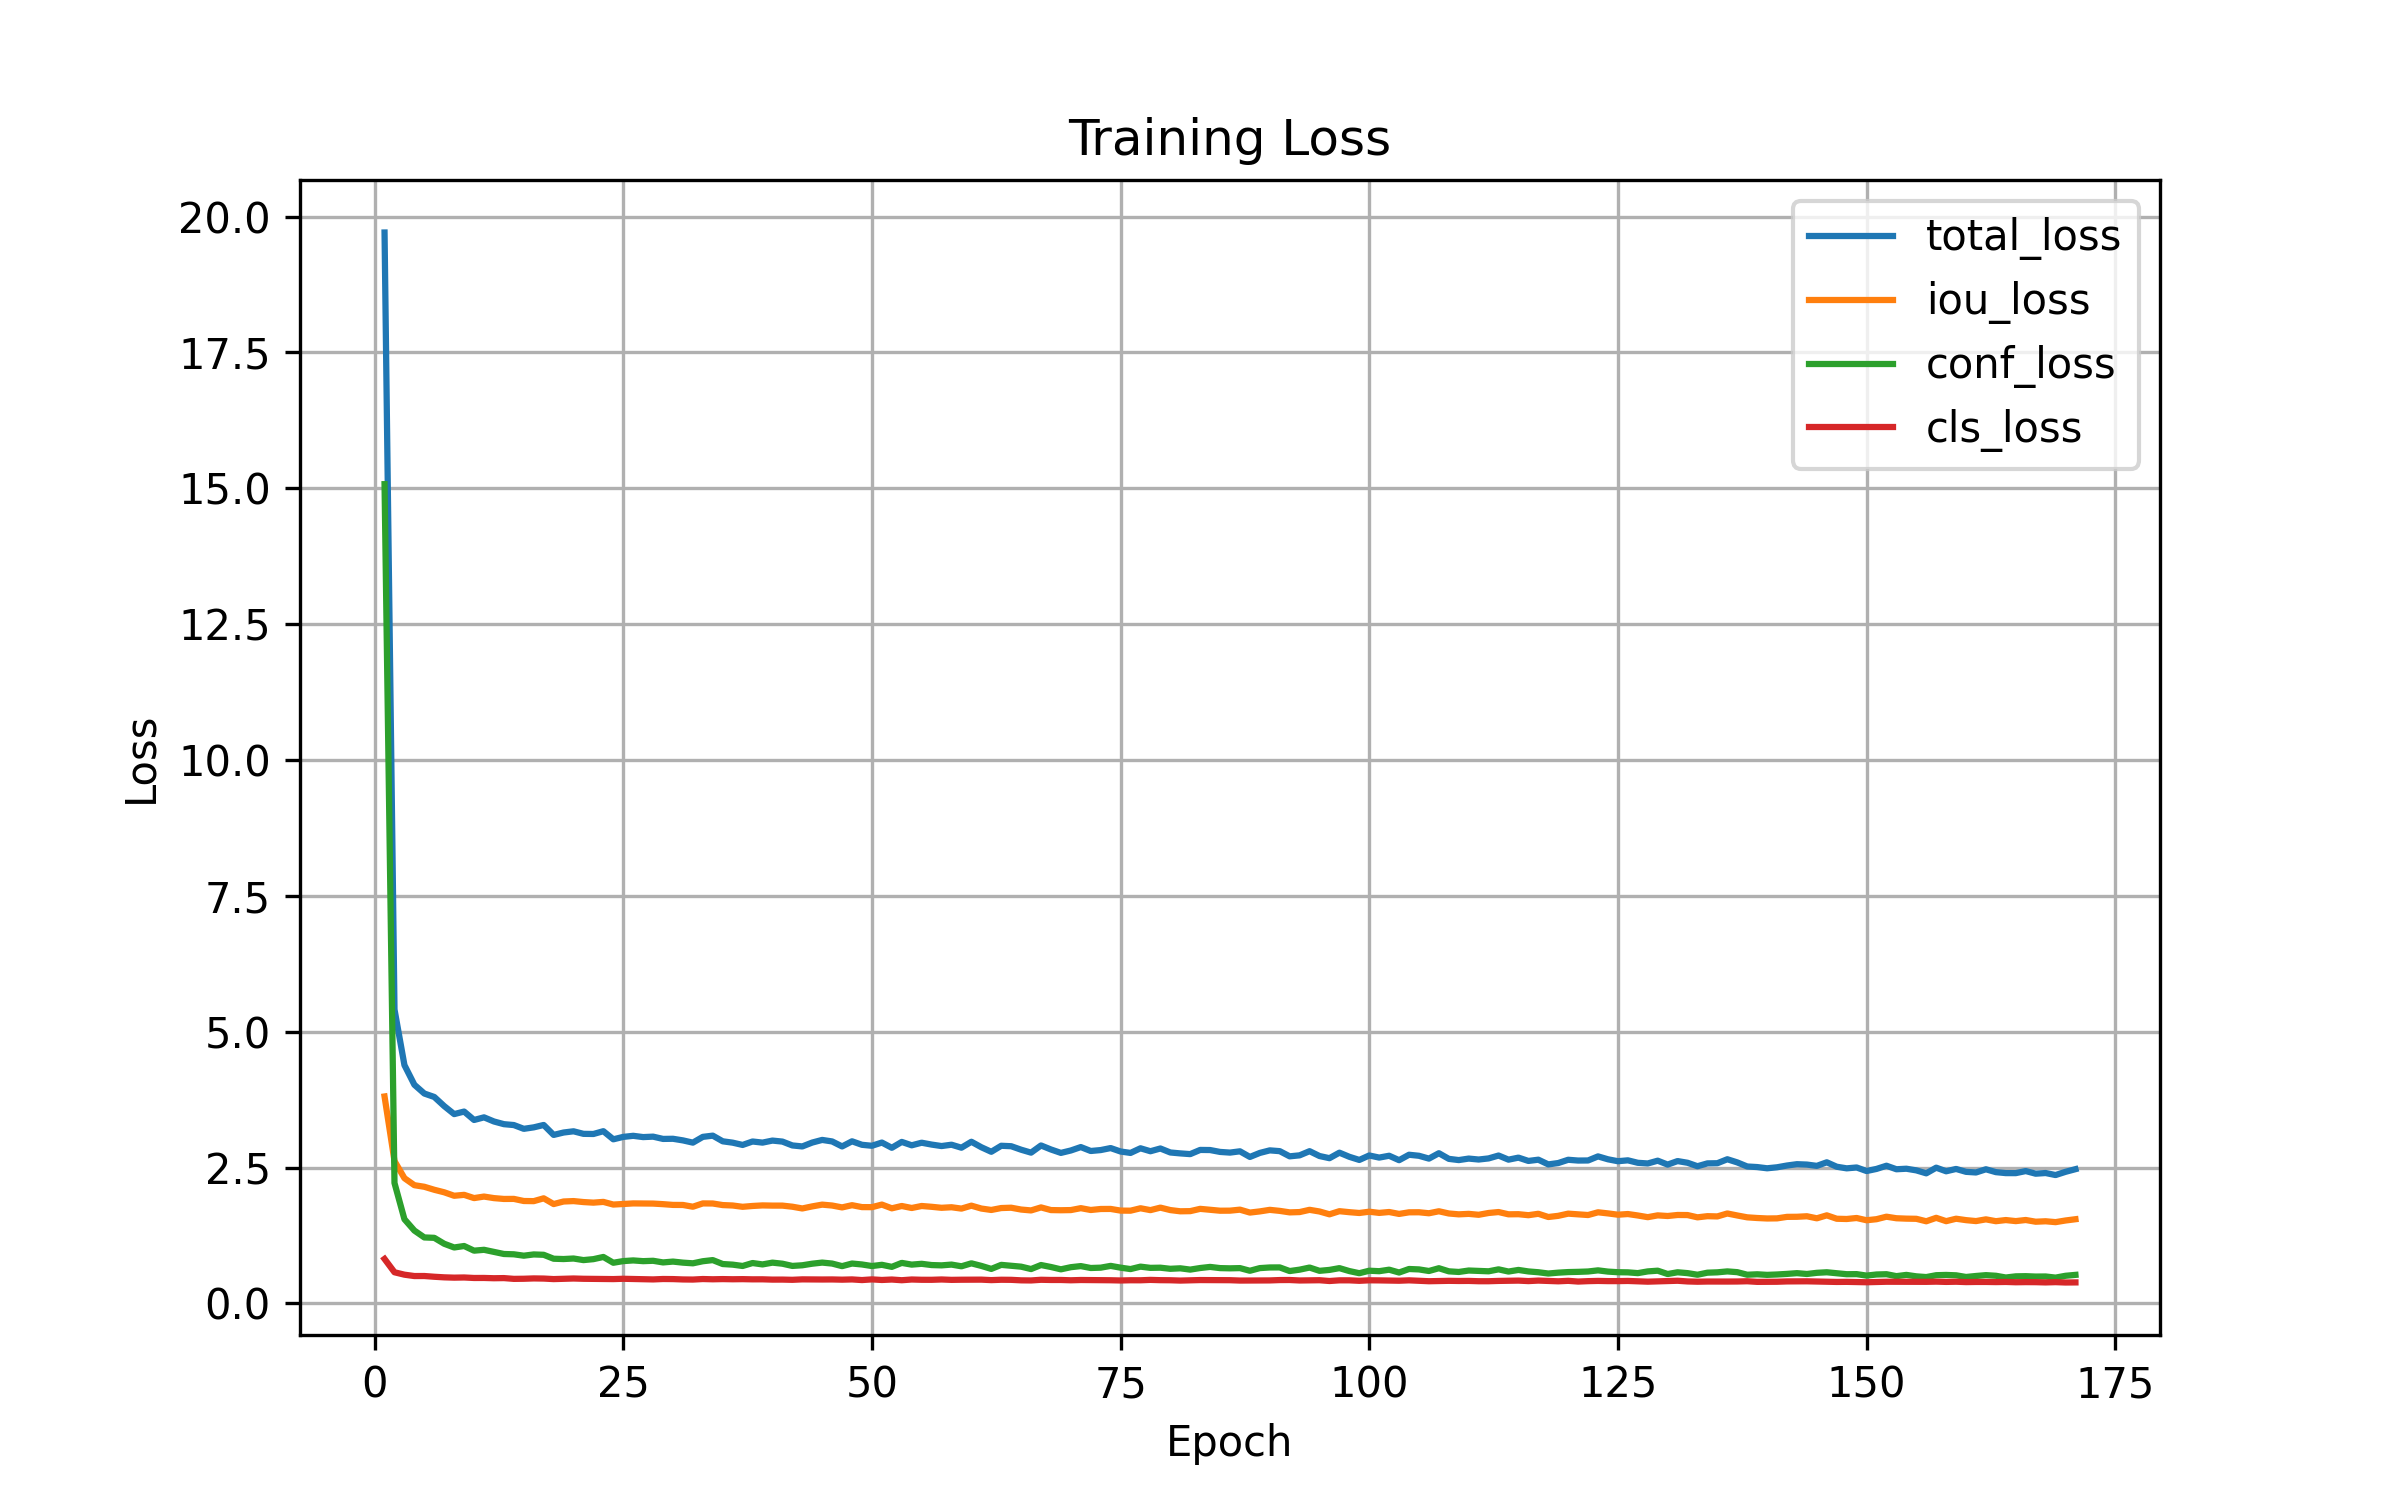
\includegraphics[width=\linewidth]{figures/images/chapter-11/licenseplate/v1/loss_curve.png}
\caption{Training loss}
\end{subfigure}
\hfill
\begin{subfigure}{0.48\textwidth}
\centering
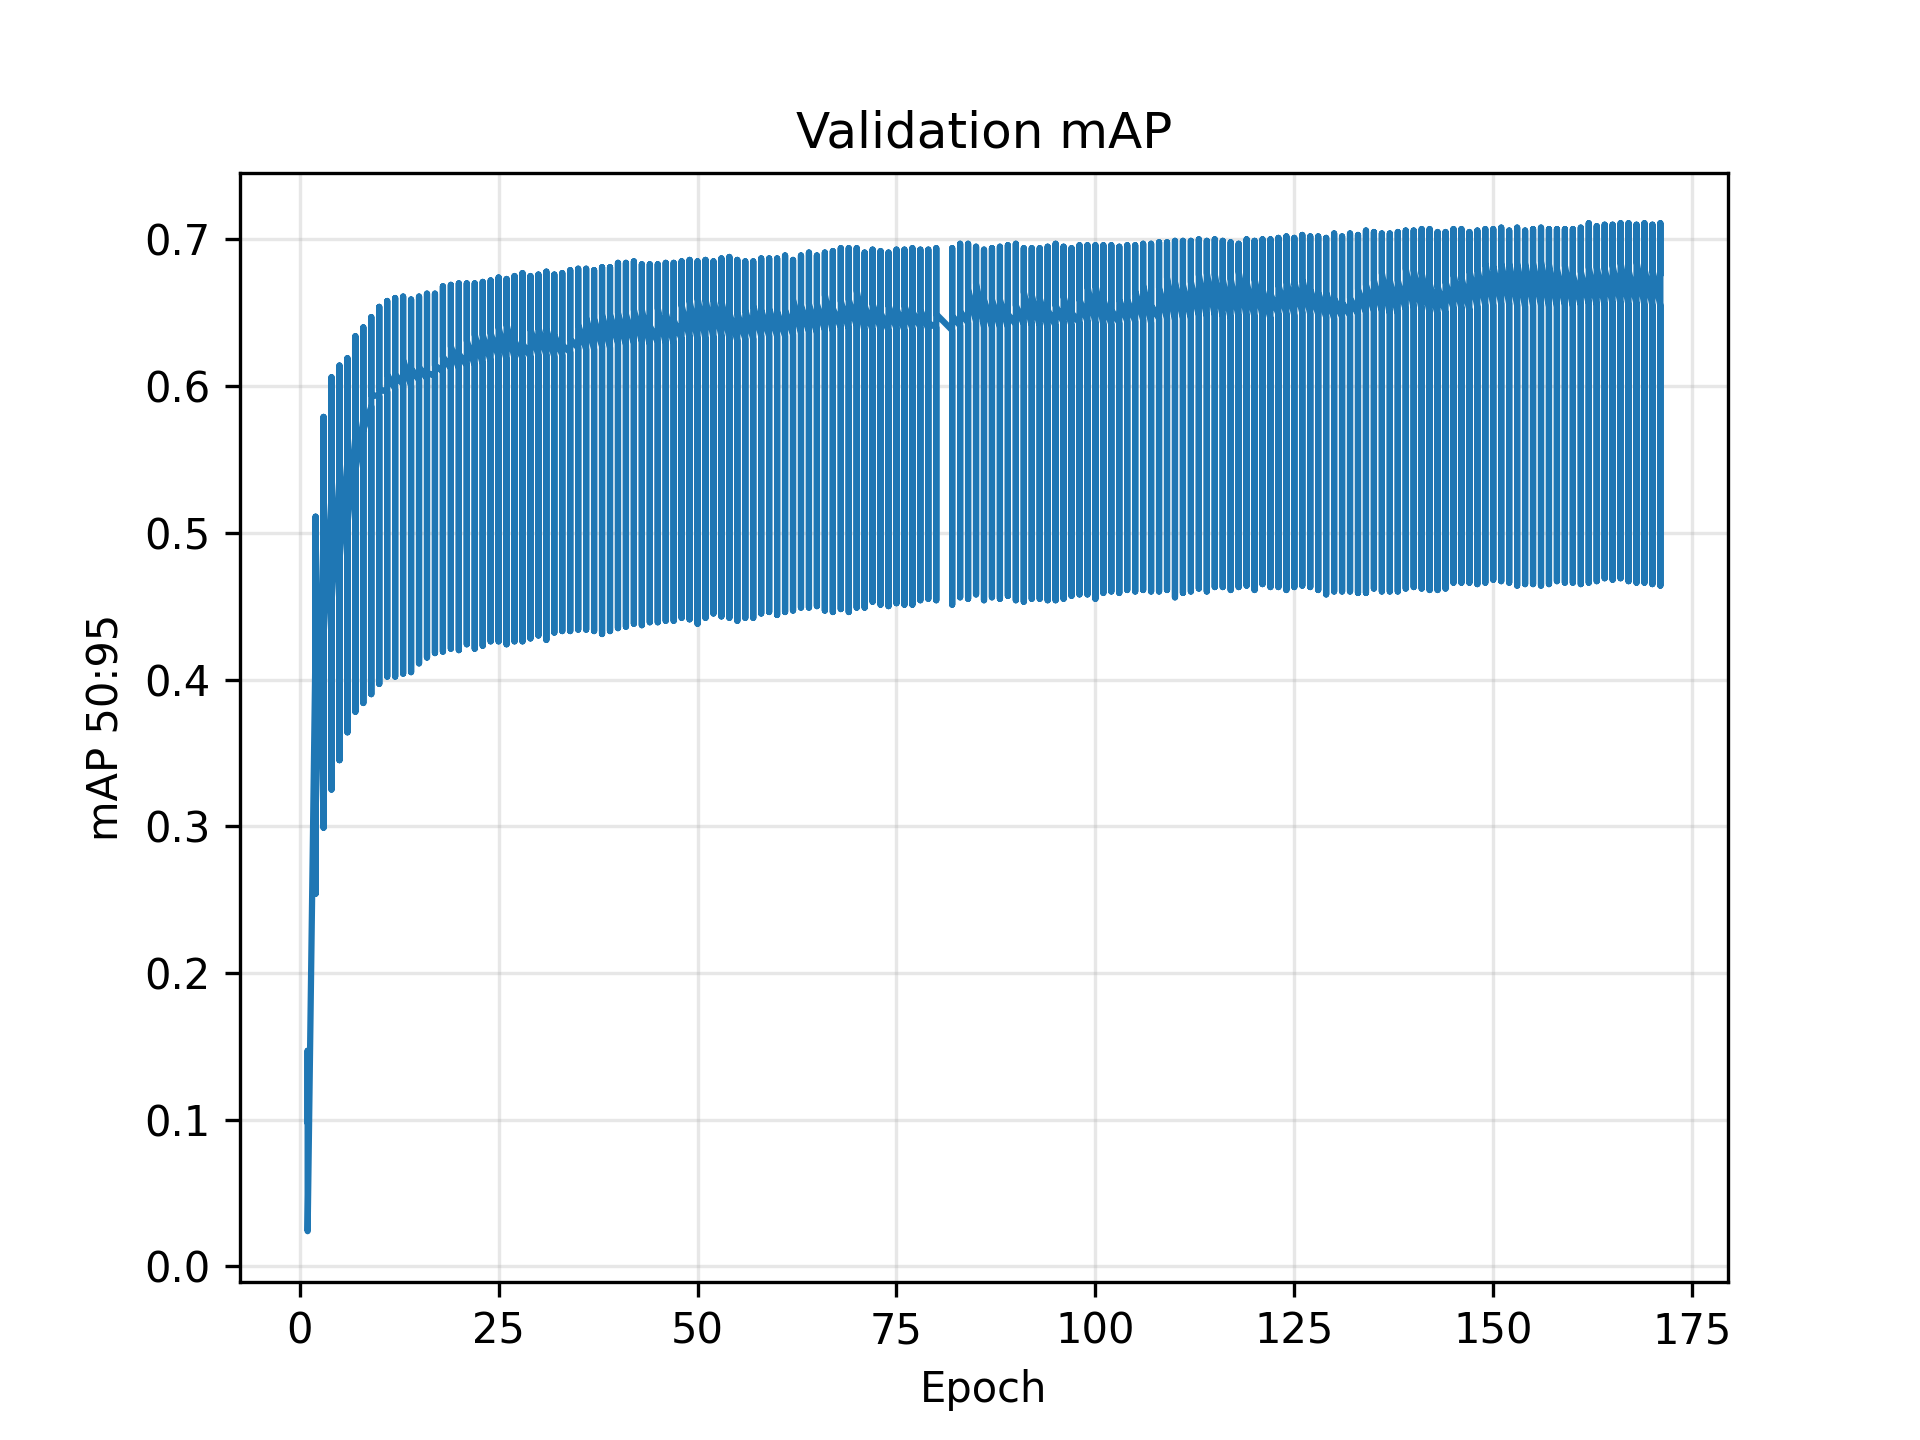
\includegraphics[width=\linewidth]{figures/images/chapter-11/licenseplate/v1/map_curve.png}
\caption{Validation mAP}
\end{subfigure}

\vspace{0.4cm}

\begin{subfigure}{0.50\textwidth}
\centering
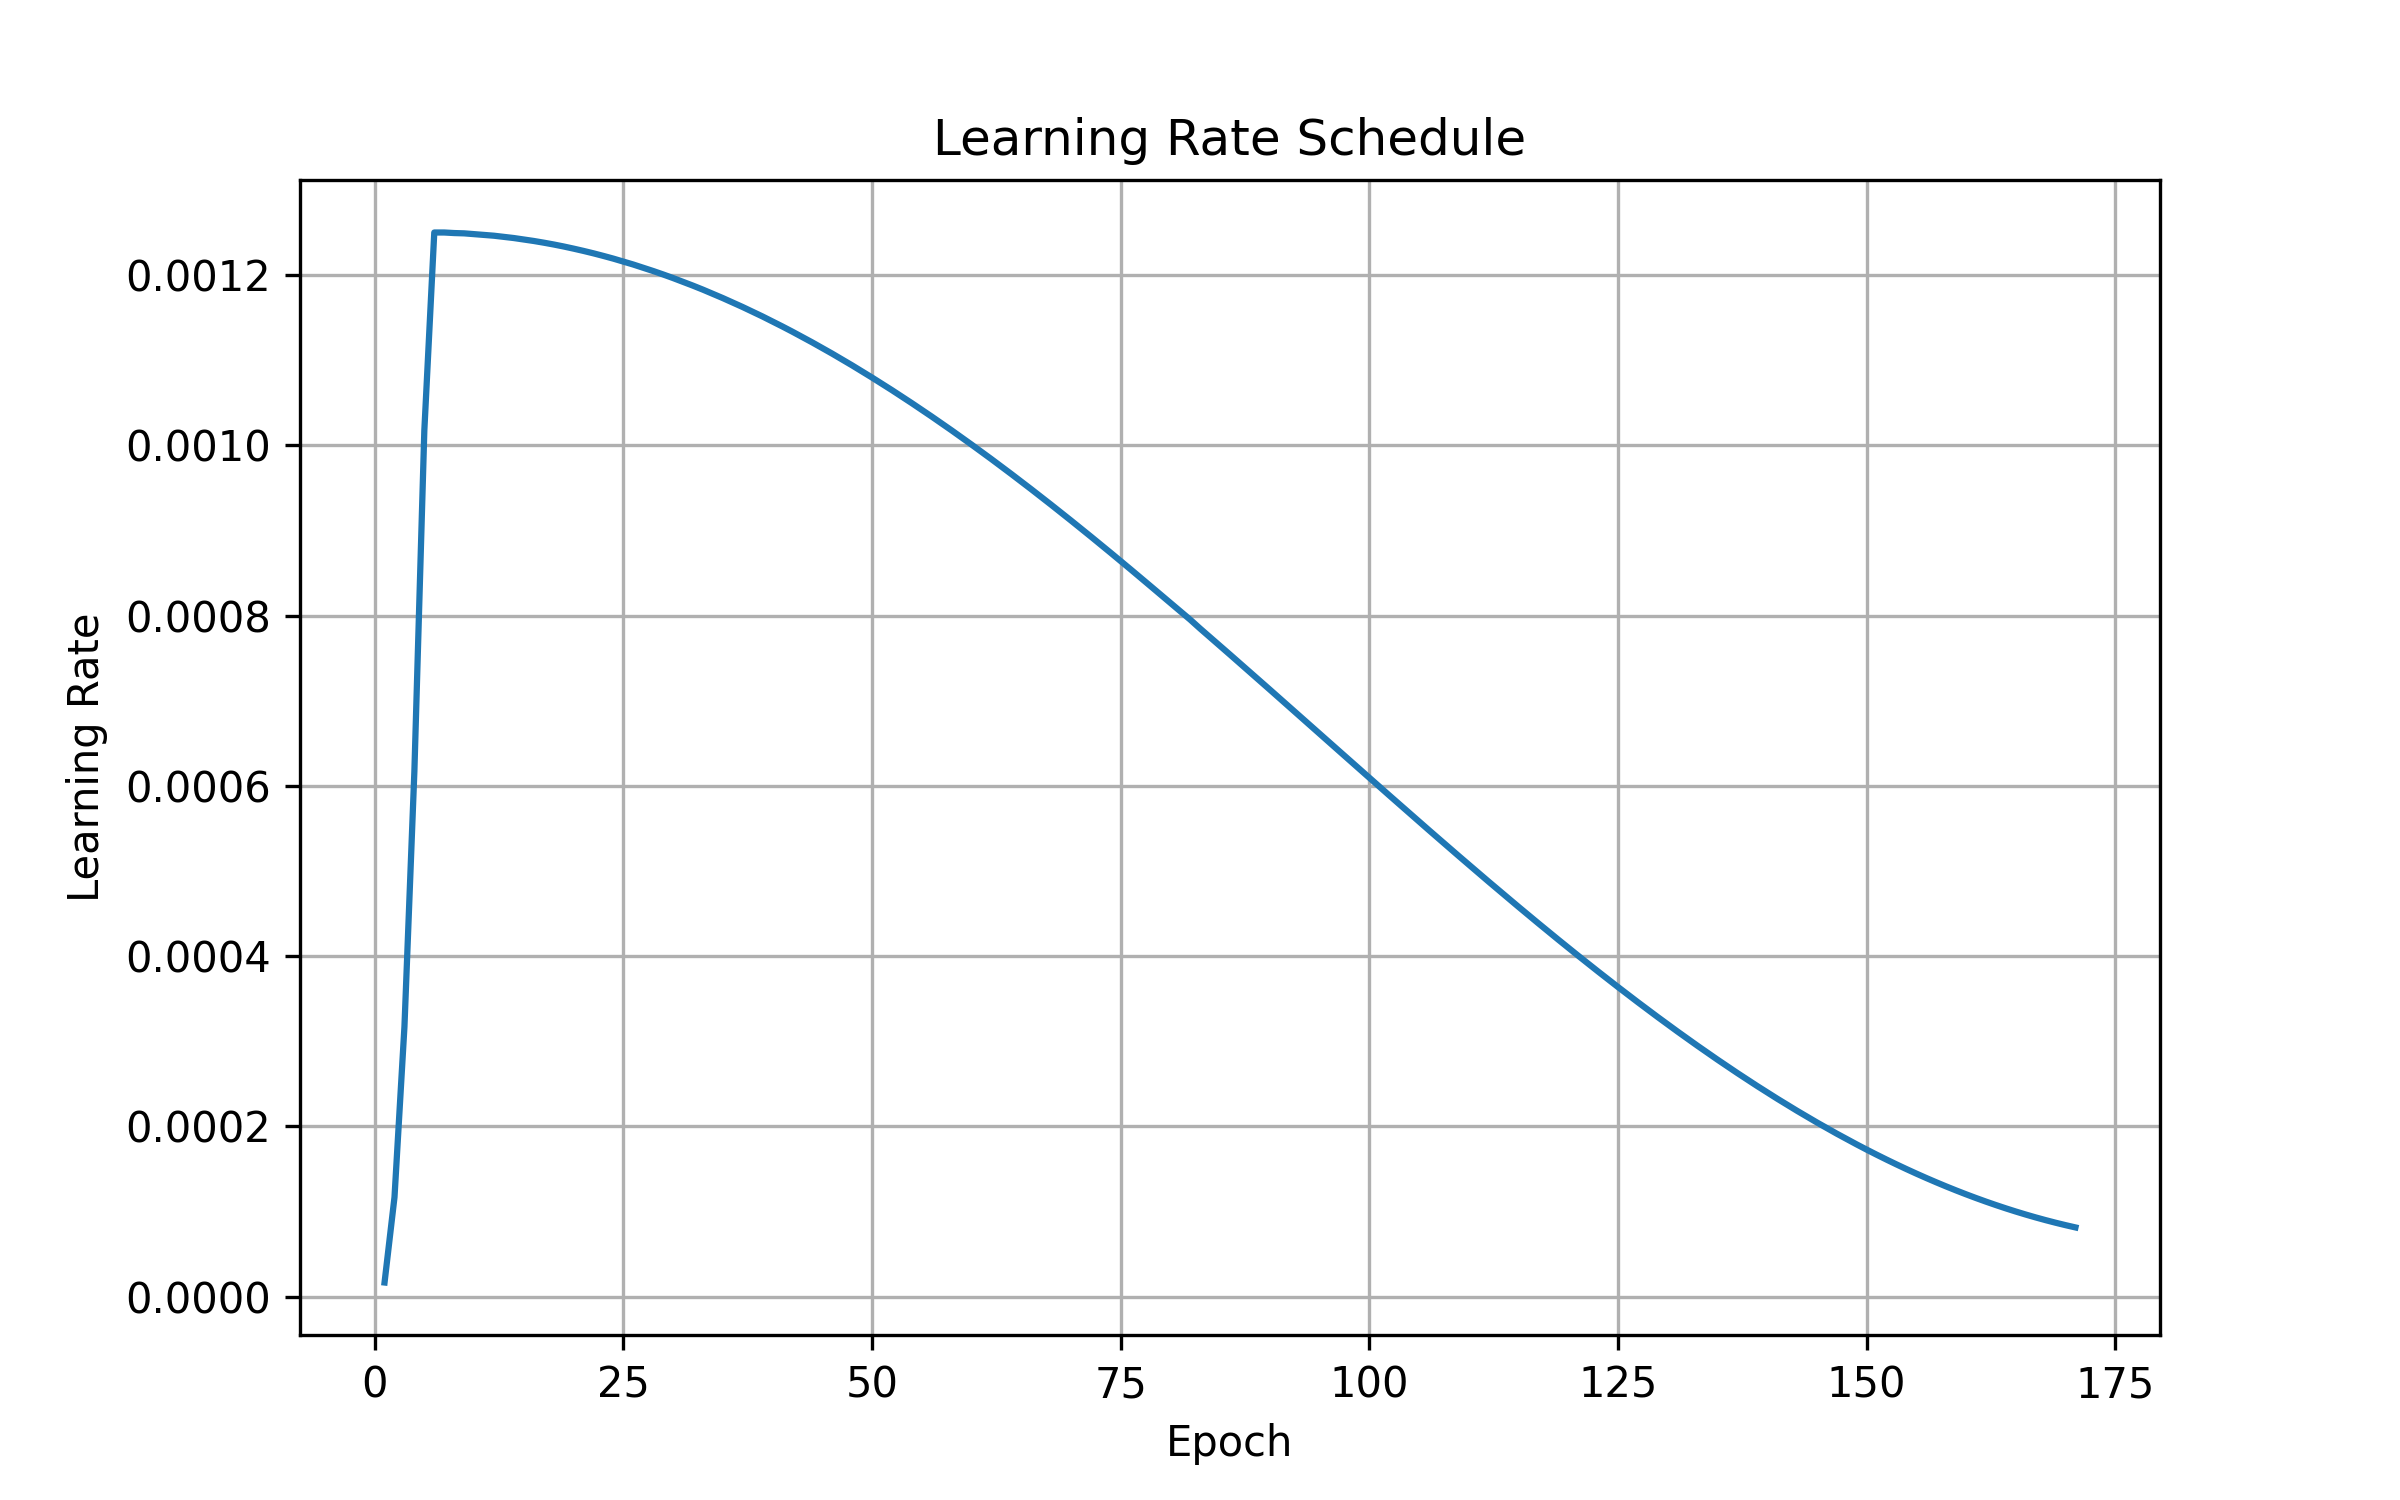
\includegraphics[width=\linewidth]{figures/images/chapter-11/licenseplate/v1/lr_curve.png}
\caption{Learning rate schedule}
\end{subfigure}

\caption{Training behaviour of model v1.}
\label{fig:lp_training_v1}

\end{figure}

Figure~\ref{fig:lp_training_v0} and Figure~\ref{fig:lp_training_v1} show the
training behaviour of the two license plate detection models. For both models,
the training loss decreases rapidly during the first epochs and then gradually
stabilizes, indicating stable optimization.

The validation mAP increases quickly at the beginning of training and then
continues to improve more gradually. Model v0 was trained for the full 200
epochs, while model v1 stopped earlier at approximately 175 epochs due to the
early stopping criterion. In both cases, the learning rate follows the expected
warm-up and decay schedule.







\subsection{Precision--Recall Analysis}

\begin{figure}[H]
\centering

\begin{subfigure}{0.48\textwidth}
\centering
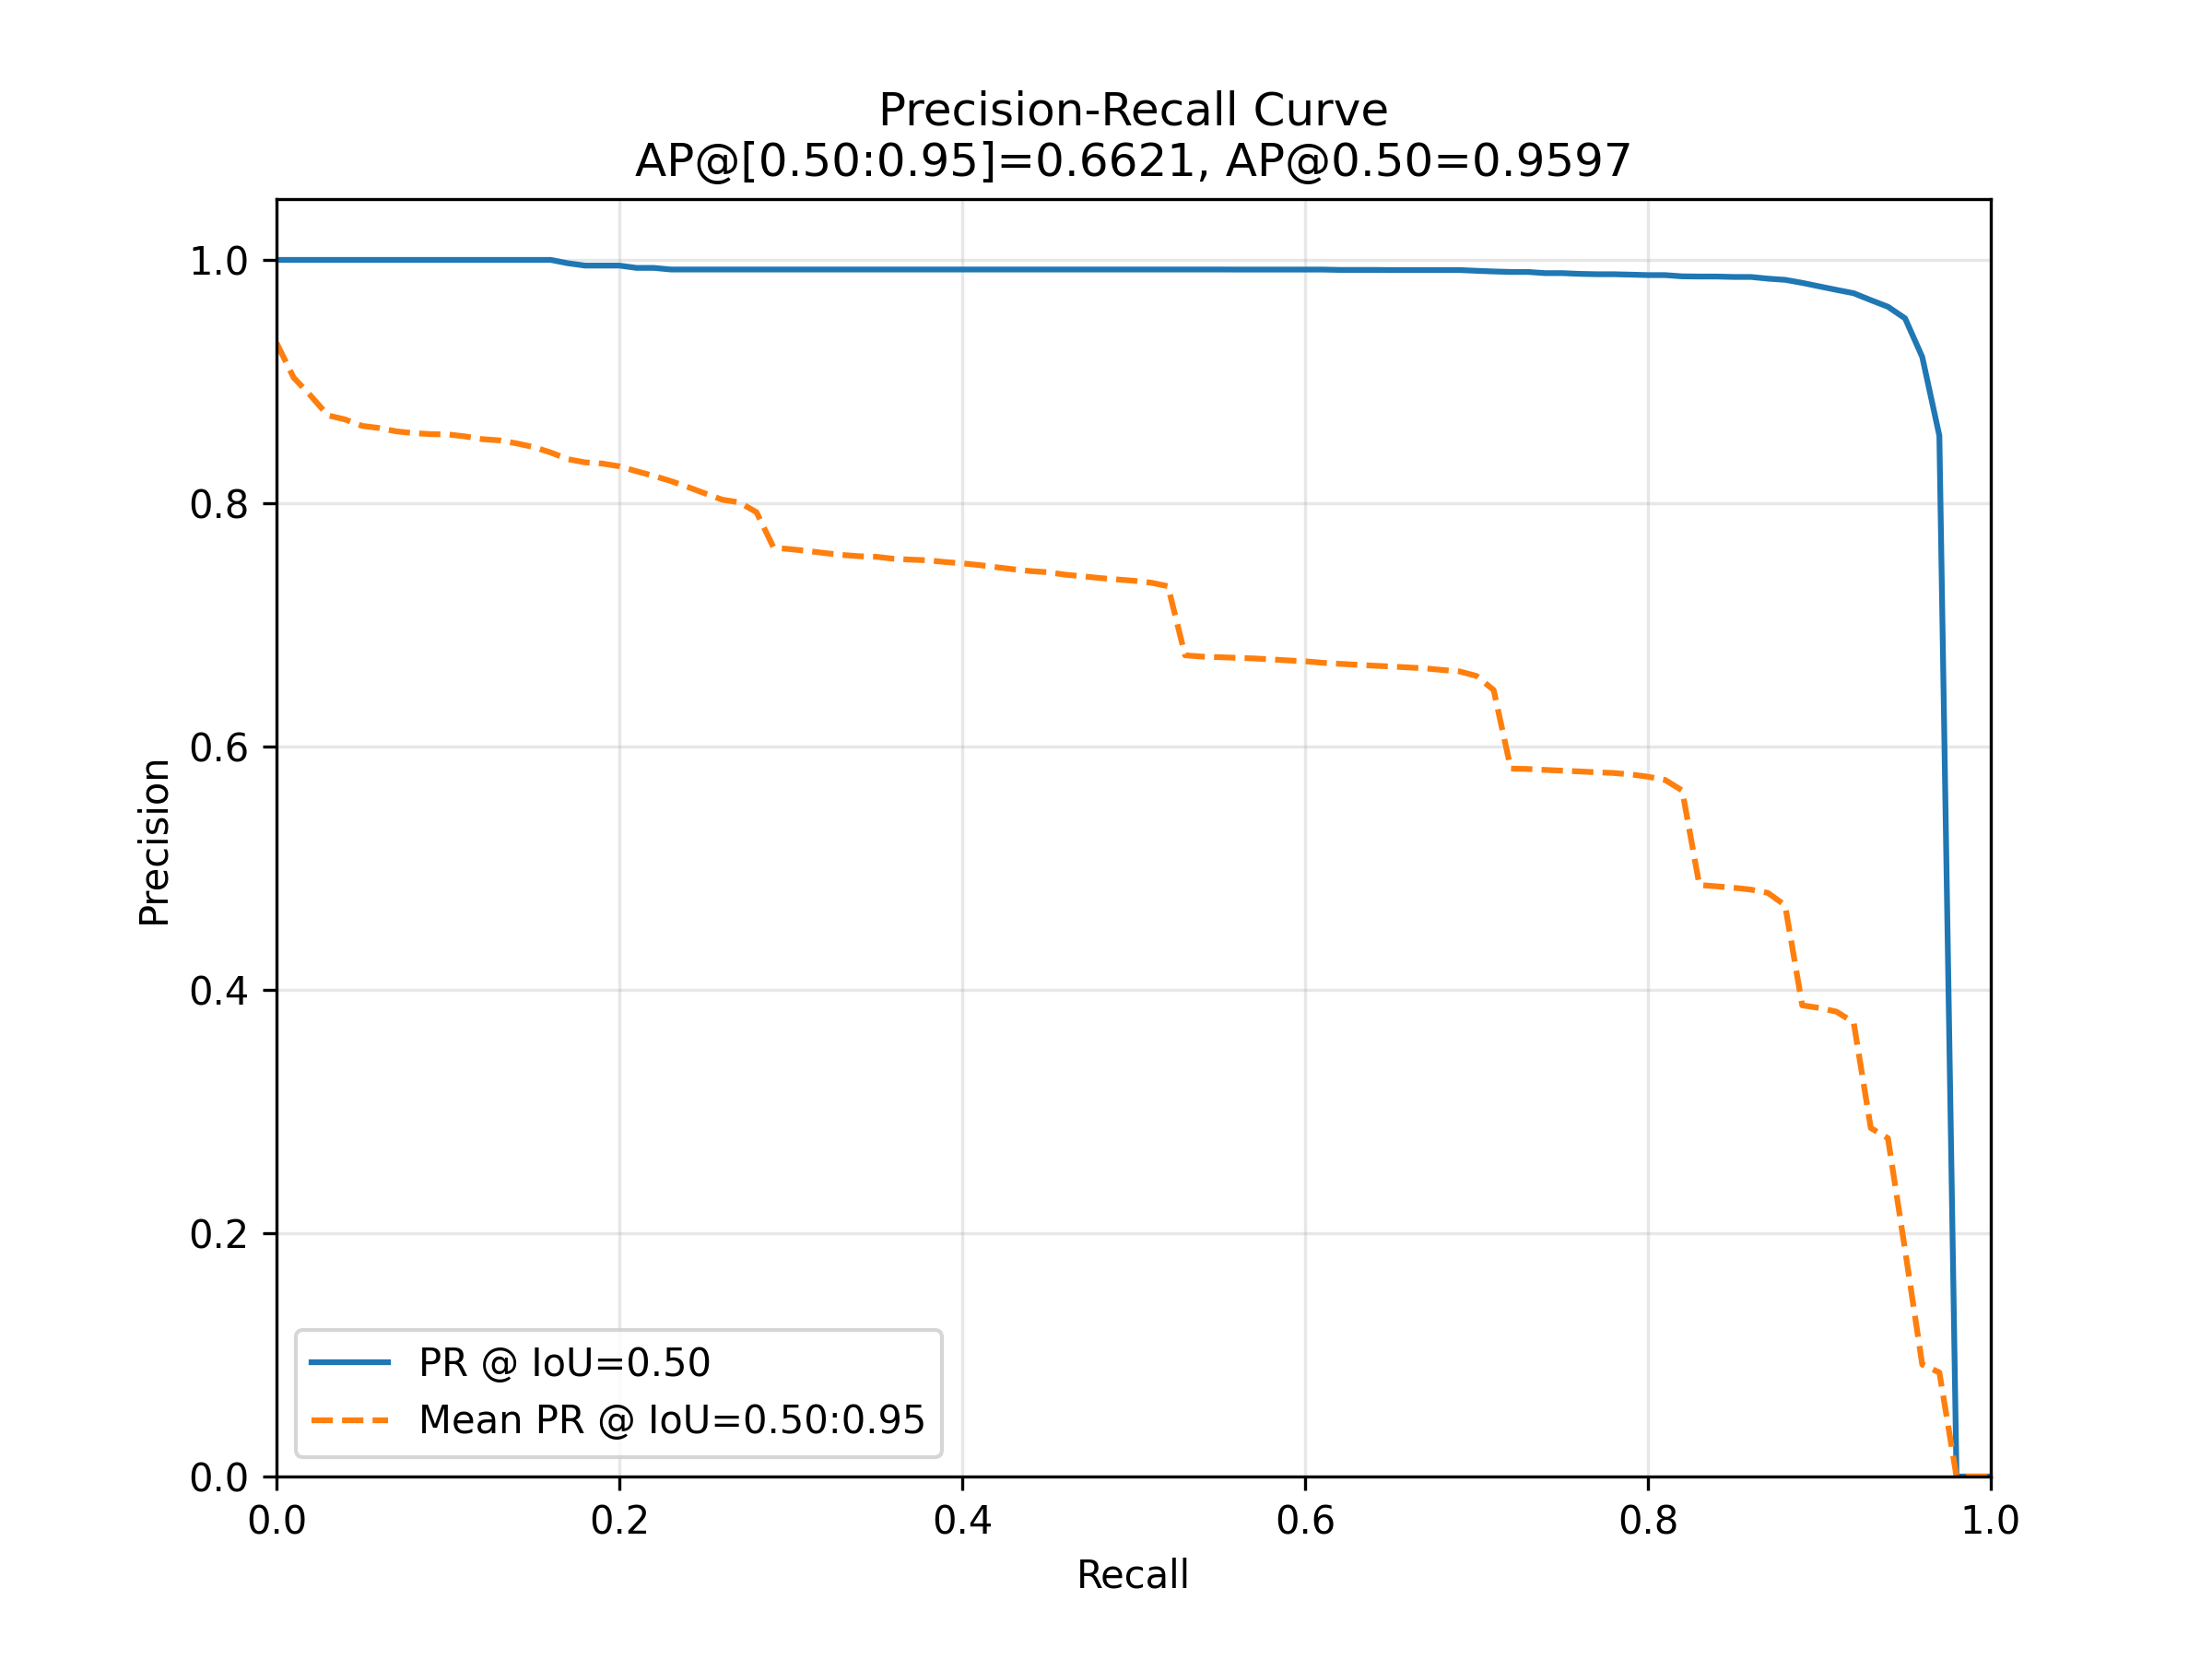
\includegraphics[width=\linewidth]{figures/images/chapter-11/licenseplate/v0/pr_curve.png}
\caption{V0 configuration.}
\end{subfigure}
\hfill
\begin{subfigure}{0.48\textwidth}
\centering
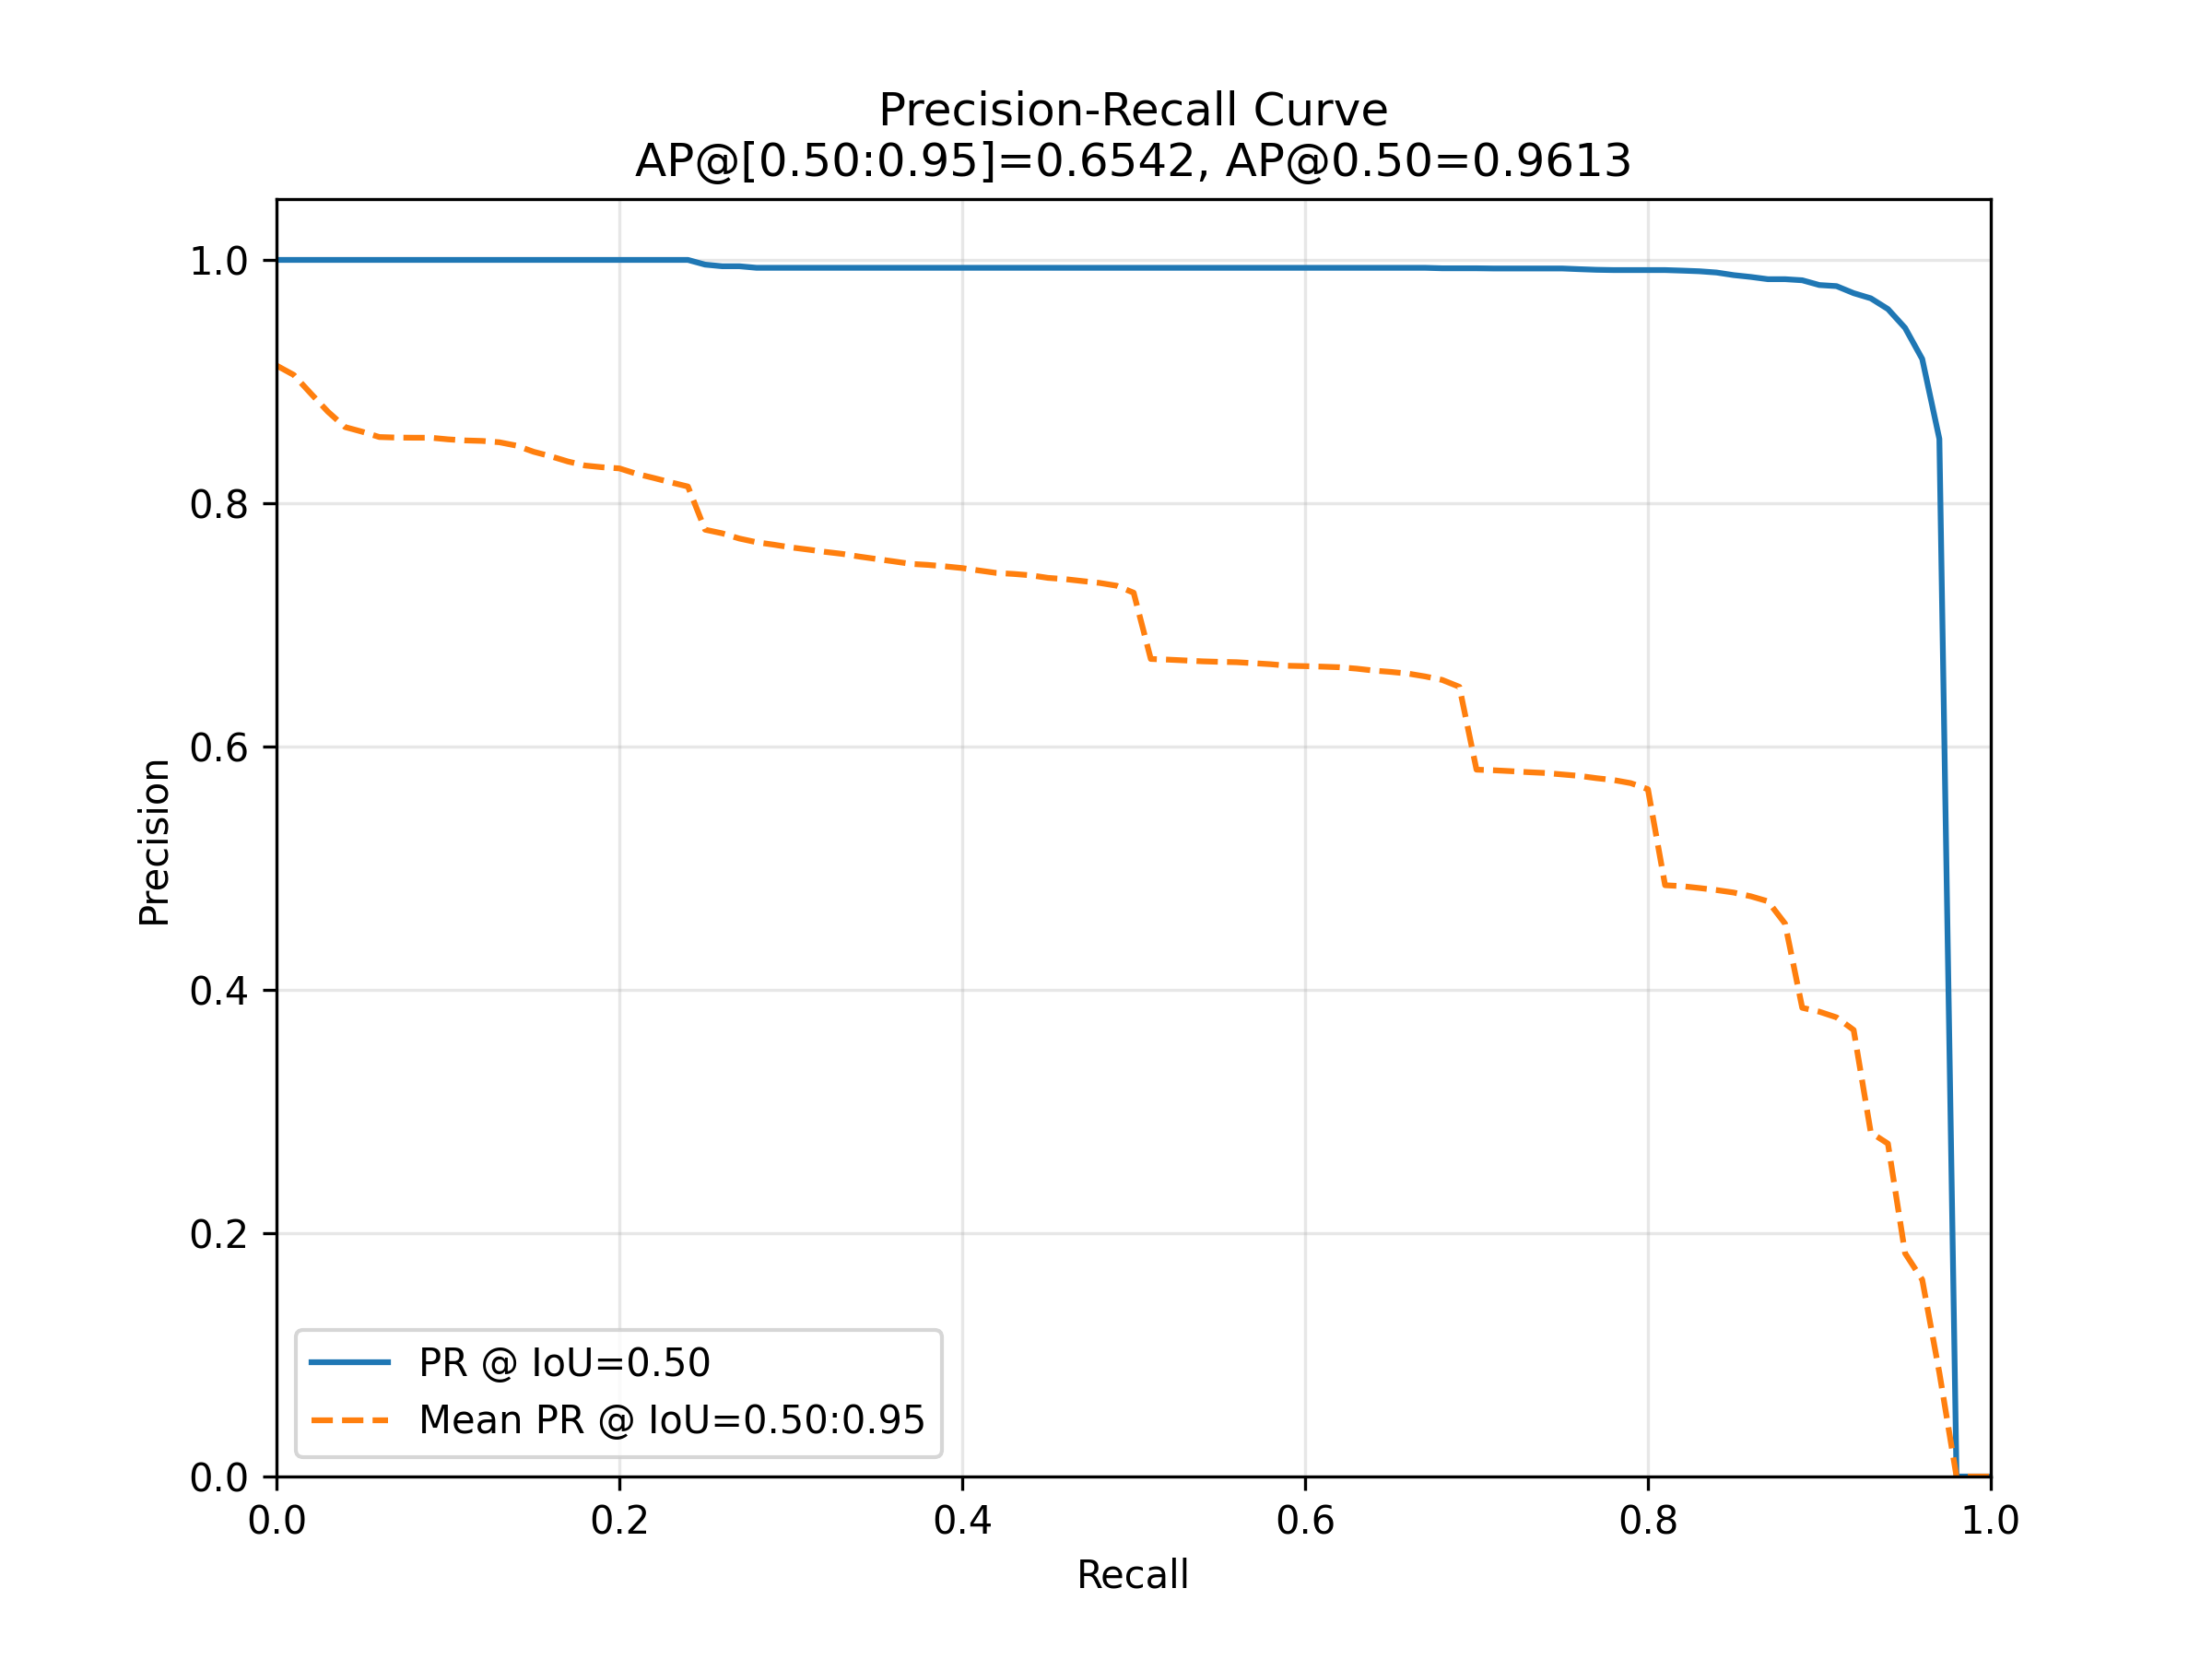
\includegraphics[width=\linewidth]{figures/images/chapter-11/licenseplate/v1/pr_curve.png}
\caption{V1 configuration.}
\end{subfigure}

\caption{Side-by-side comparison of the precision--recall curves for the v0 and v1 configurations.}
\label{fig:lp_pr_curves_licenseplate} 
\end{figure}

Figure~\ref{fig:lp_pr_curves_licenseplate} shows the precision--recall curves for the two
license plate detection models. Both configurations achieve a high AP@0.50,
with v0 reaching 0.9597 and v1 reaching 0.9613. This indicates strong detection
performance for both models at an IoU threshold of 0.50.

The AP@0.50:0.95 values are also similar, with v0 achieving 0.6621 and v1
achieving 0.6542. Although v1 performs slightly better at AP@0.50, v0 obtains a
slightly higher score across the stricter IoU range. Overall, the
precision--recall analysis shows that the two configurations perform similarly,
with only small differences between them.





\subsection{Confusion Matrix Analysis}

\begin{figure}[H]
\centering
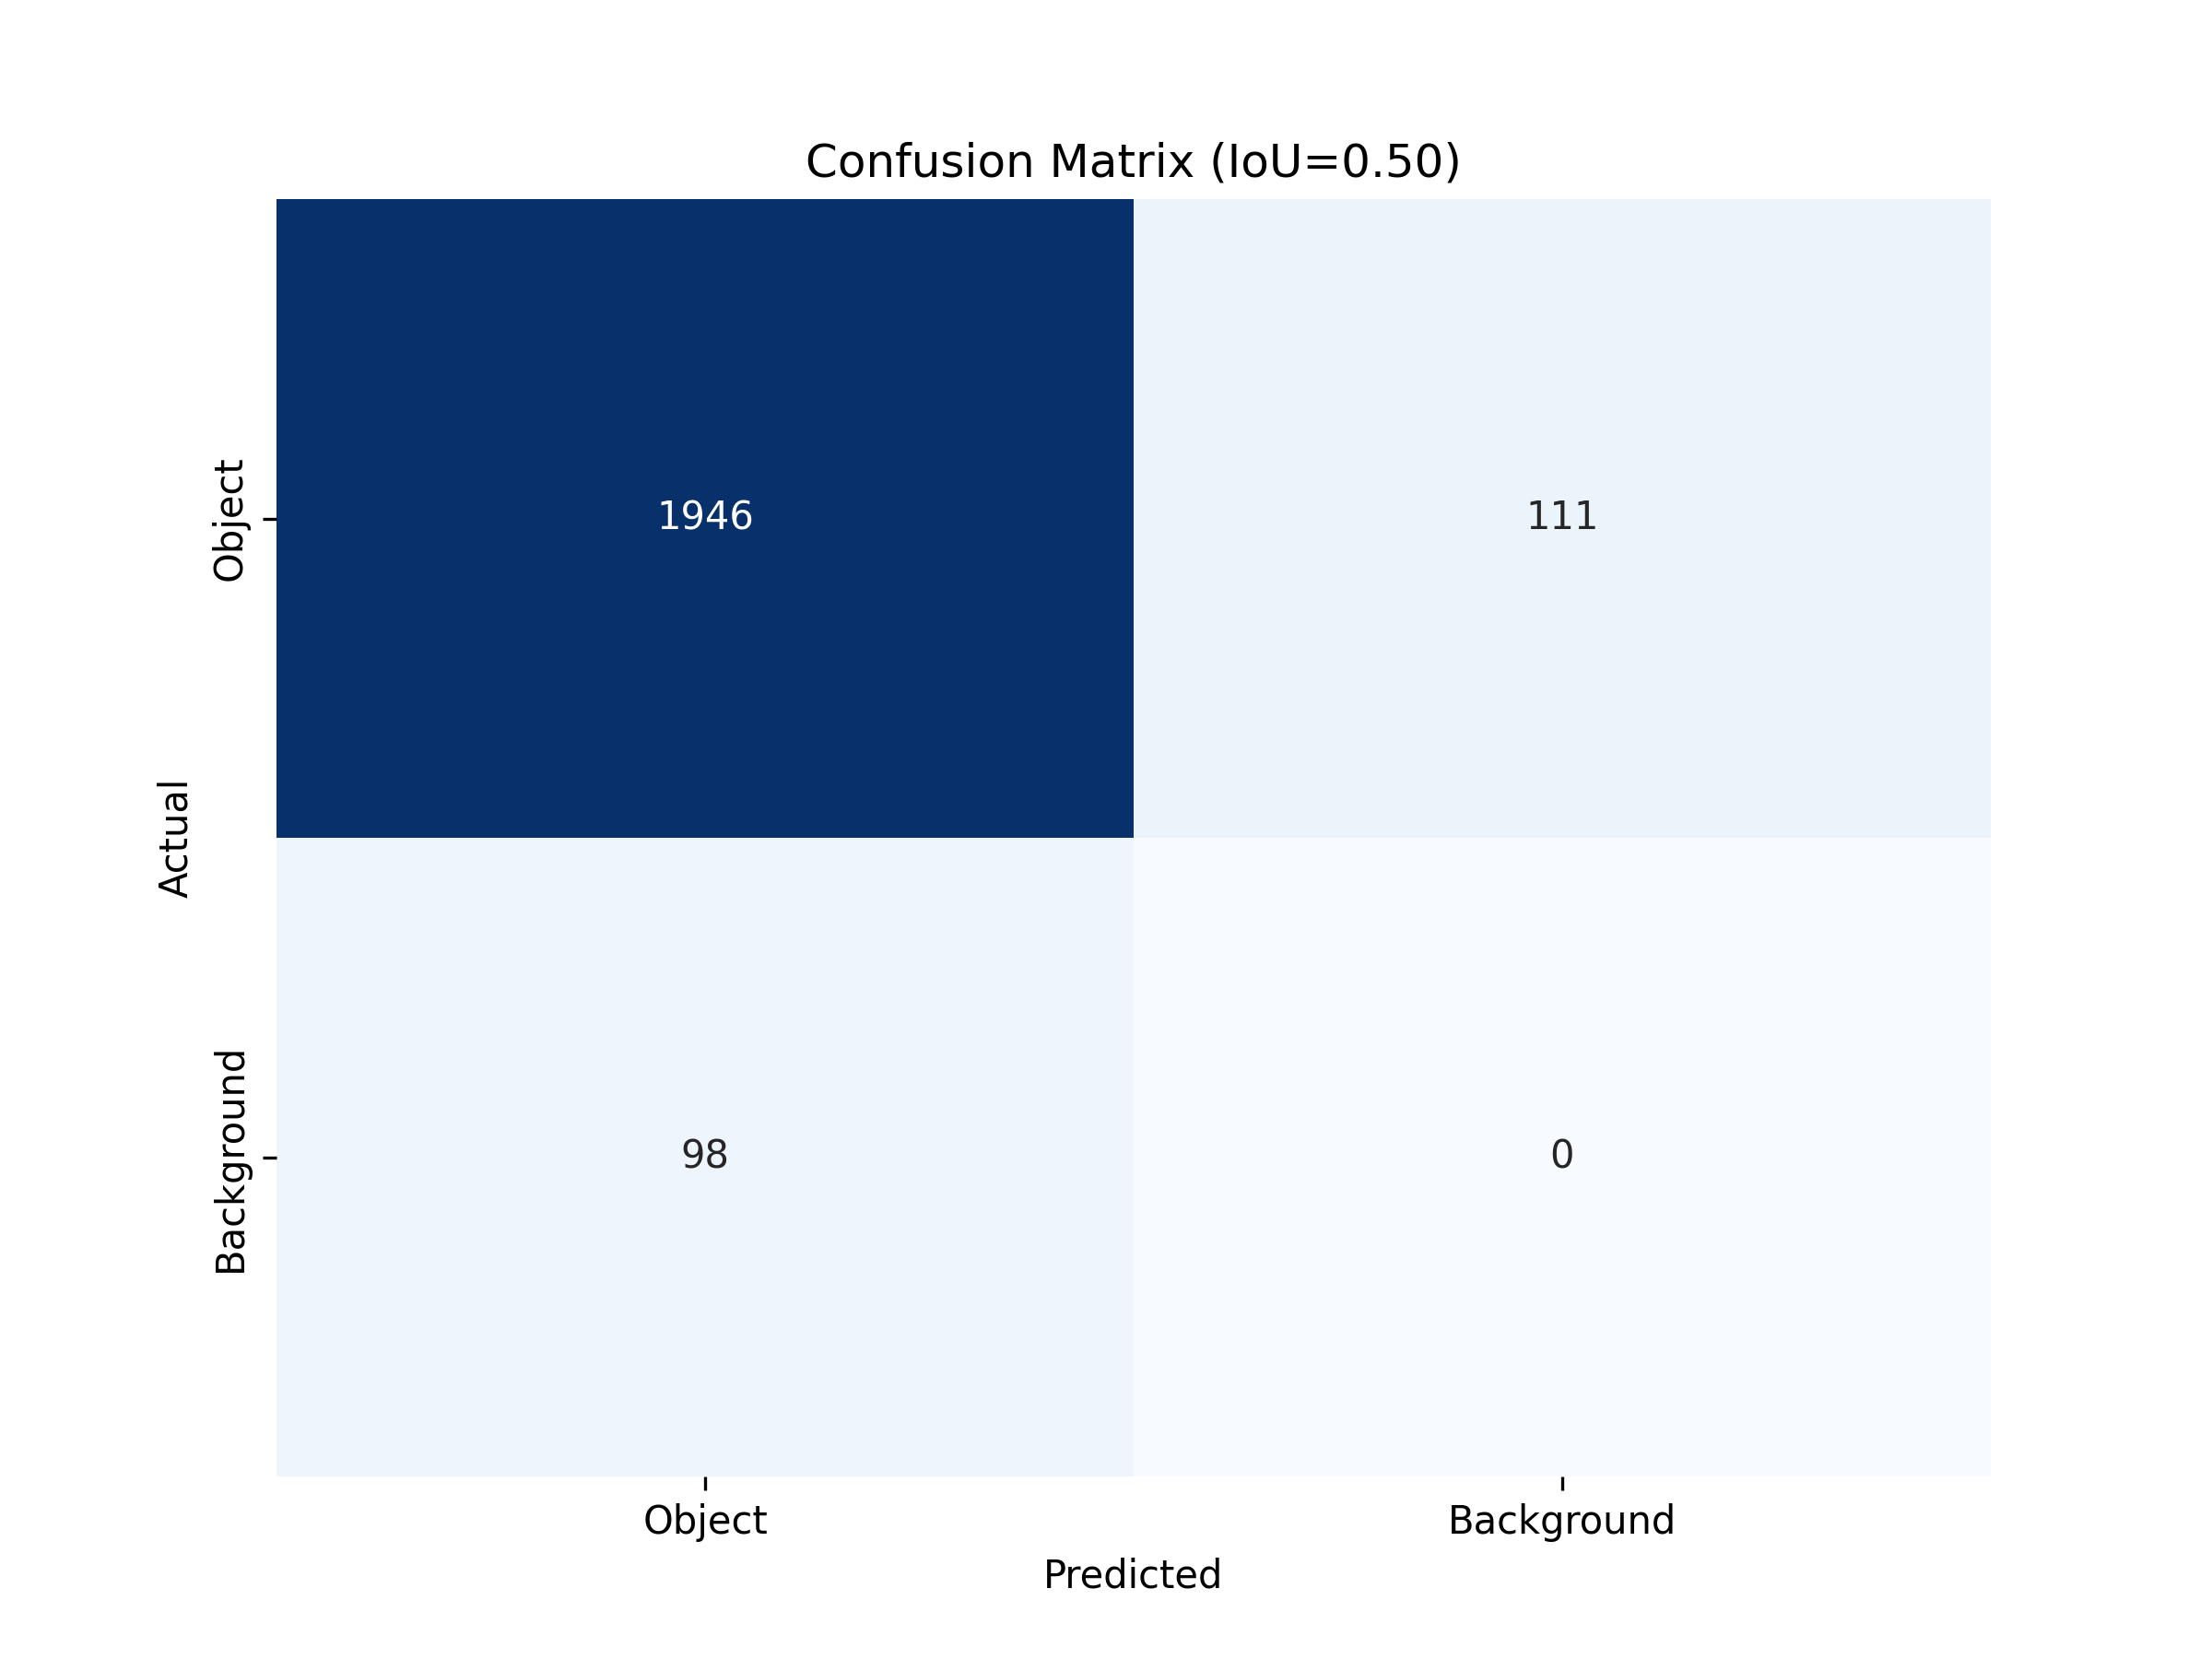
\includegraphics[width=12cm]{figures/images/chapter-11/licenseplate/v0/confusion_matrix_0.3.png}
\caption{Confusion matrix for the v0 configuration.}
\label{fig:lp_confusion_matrix_v0}
\end{figure}

\begin{figure}[H]
\centering
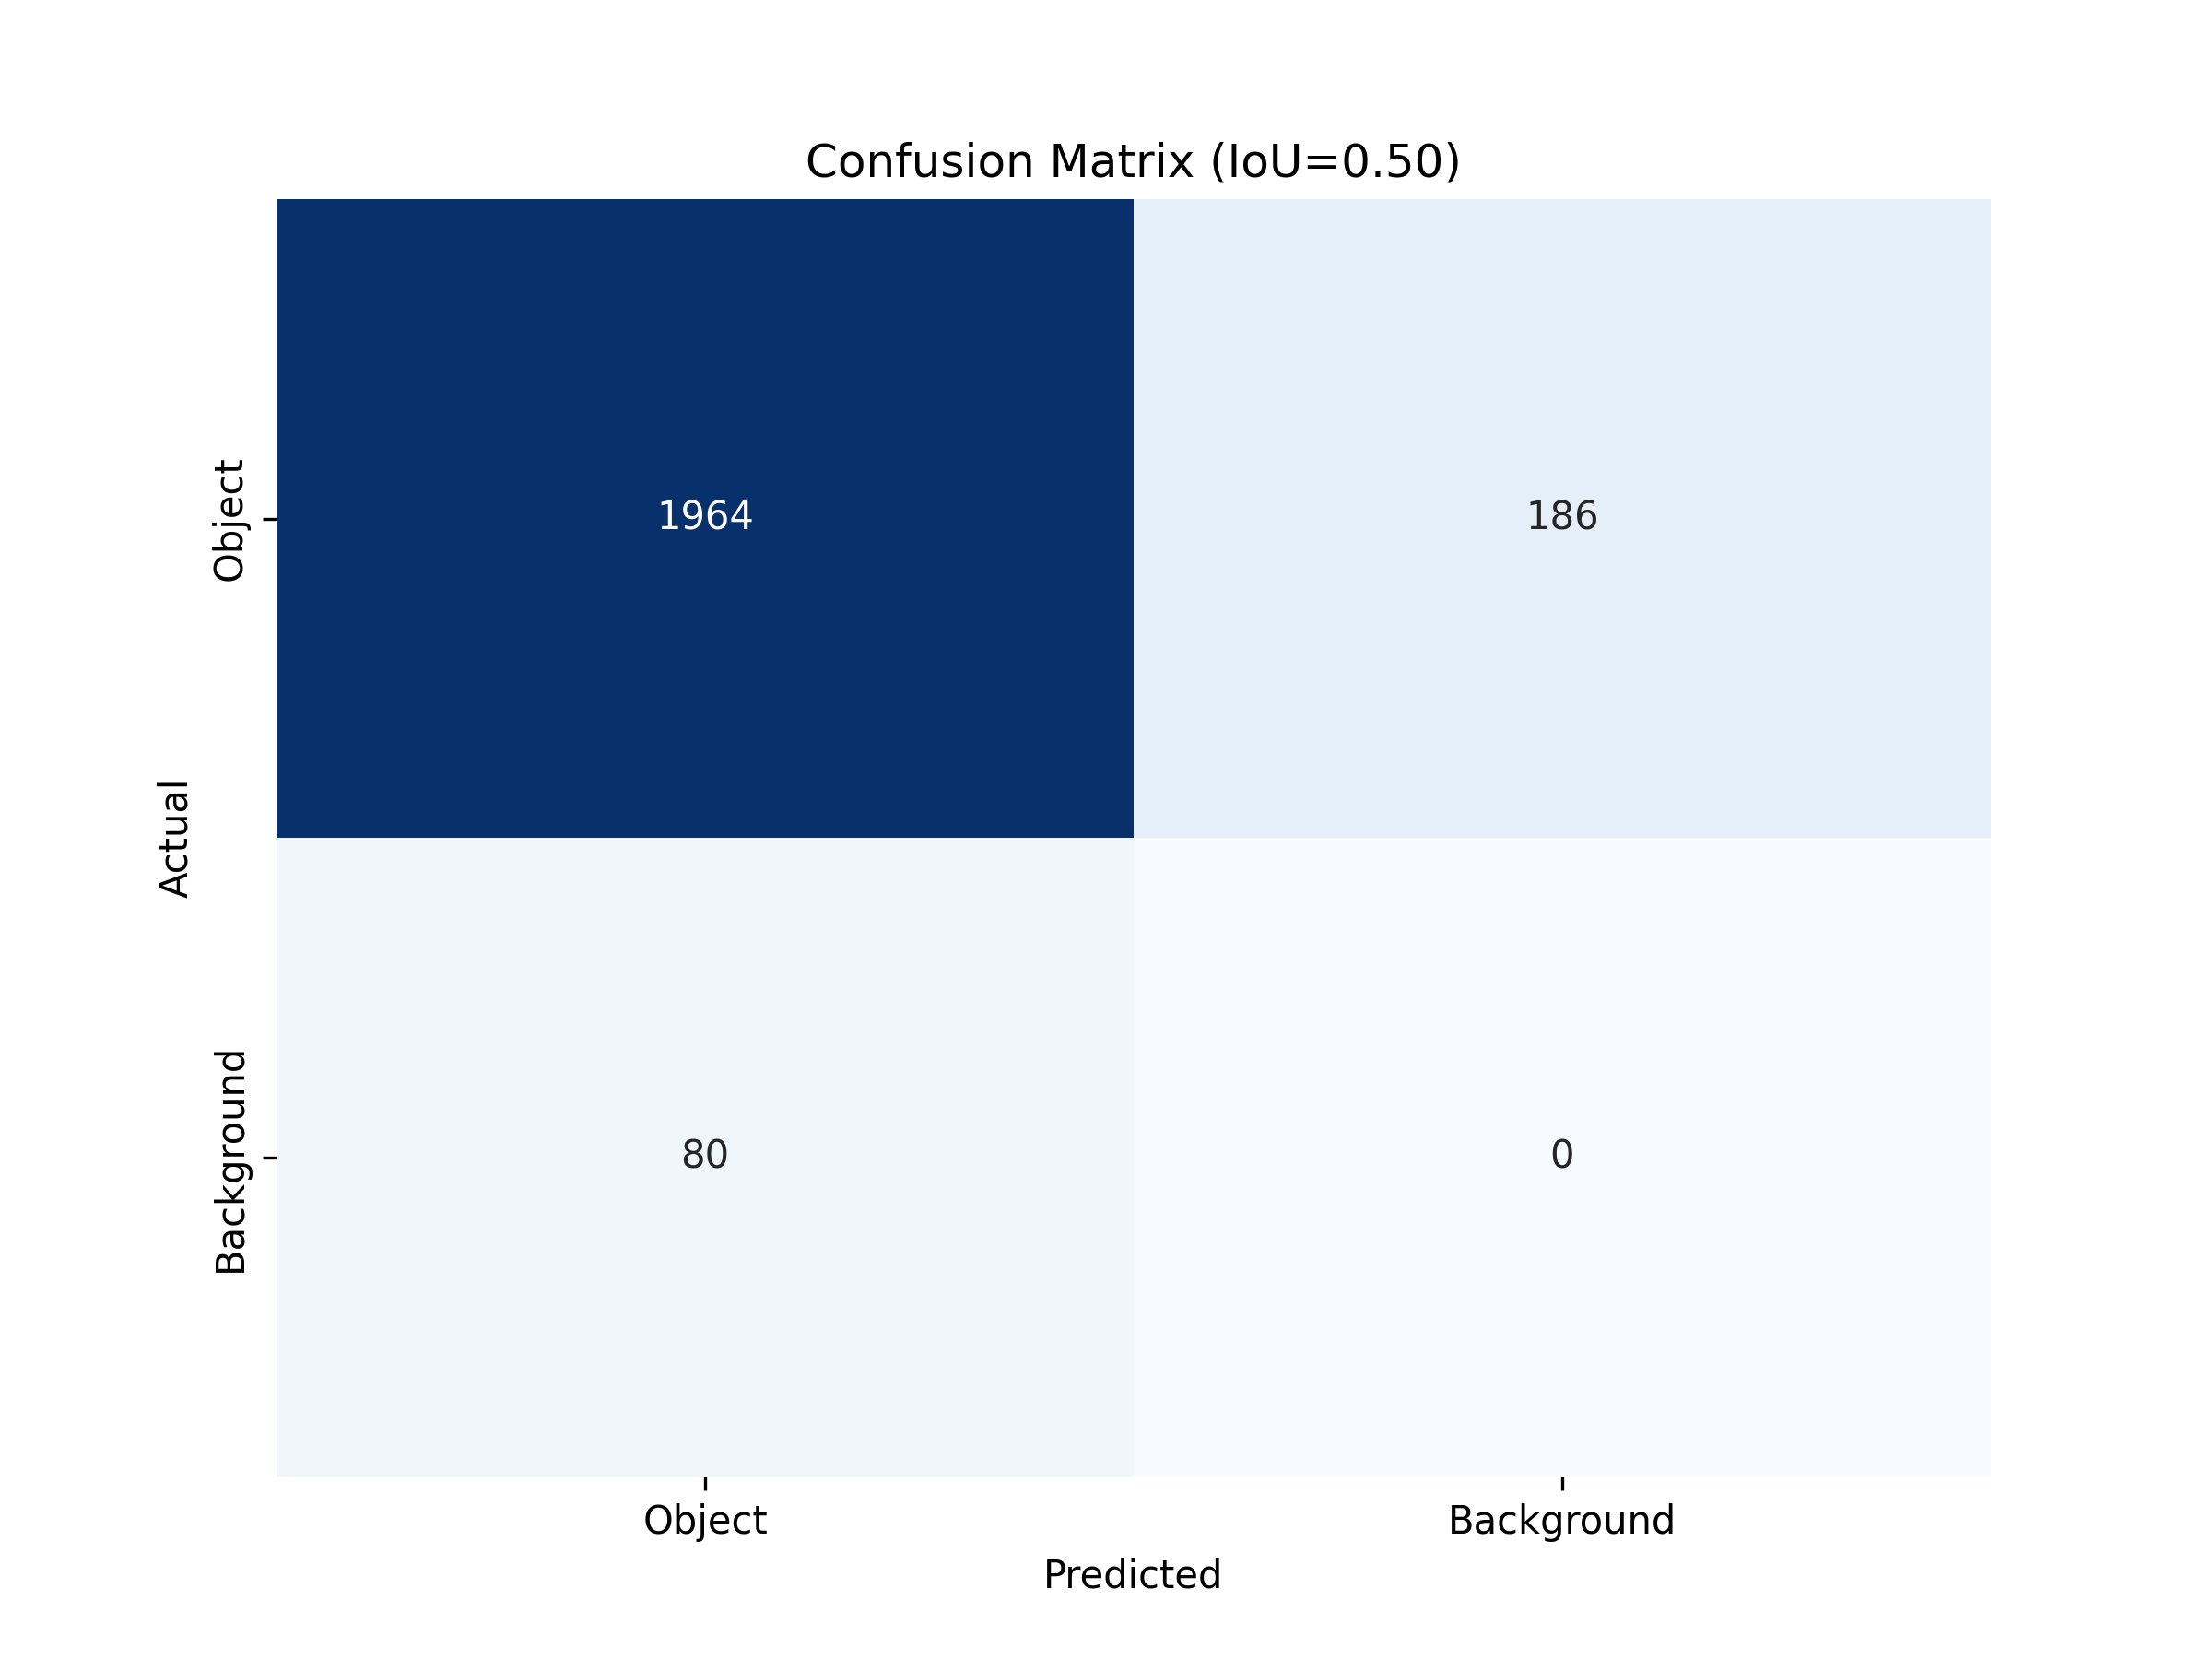
\includegraphics[width=12cm]{figures/images/chapter-11/licenseplate/v1/confusion_matrix_0.3.png}
\caption{Confusion matrix for the v1 configuration.}
\label{fig:lp_confusion_matrix_v1}
\end{figure}

Figure~\ref{fig:lp_confusion_matrix_v0} and
Figure~\ref{fig:lp_confusion_matrix_v1} show the confusion matrices for the two
license plate detection models at an IoU threshold of 0.50.

The confusion matrix values do not directly match the number of test images
because object detection is evaluated at the object level. Each image may
contain multiple license plates and multiple predicted bounding boxes.
Therefore, the matrix counts detections and missed objects rather than images.

The F1-score was calculated as the harmonic mean of precision and recall:
\[
F1 = 2 \cdot \frac{Precision \cdot Recall}{Precision + Recall}
\]

The v0 configuration correctly detected 1946 license plates, produced 98 false
positive detections, and missed 111 license plates. This resulted in a
precision of 0.9521, a recall of 0.9460, and an F1-score of 0.9490.

The v1 configuration correctly detected 1964 license plates and produced fewer
false positives, with 80 false detections. However, it also missed more license
plates, with 186 false negatives. This resulted in a slightly higher precision
of 0.9609, but a lower recall of 0.9135 and an F1-score of 0.9366.

\begin{align*}
Precision_{v0} &= \frac{1946}{1946 + 98} \approx 0.9521,
&
Recall_{v0} &= \frac{1946}{1946 + 111} \approx 0.9460,
&
F1_{v0} &\approx 0.9490
\end{align*}

\begin{align*}
Precision_{v1} &= \frac{1964}{1964 + 80} \approx 0.9609,
&
Recall_{v1} &= \frac{1964}{1964 + 186} \approx 0.9135,
&
F1_{v1} &\approx 0.9366
\end{align*}

Overall, v1 is slightly more precise, while v0 achieves better recall and a
higher F1-score. This indicates that v0 provides a better balance between
detecting license plates and avoiding false detections.

\subsection{Summary}

Both license plate detection models achieved strong detection performance on
the unseen test set. Model v1 obtained slightly higher precision, while model
v0 achieved higher recall and a higher F1-score.

Since the proposed system benefits from detecting as many license plates as
possible while still maintaining high precision, the v0 configuration was
selected as the final license plate detection model. The results show that v0
provides the best overall balance between precision, recall, and F1-score. The final barcode detection model was therefore selected for use in the proposed system.










% --------------------------------------------------------------------------------


\section{Named Entity Recognition}
\label{app:ner_evaluation}

\subsection{Training Setup}

The NER model was trained as a token classification model based on XLM-RoBERTa. Unlike the barcode and license plate models, which were trained as object detectors, the NER component addressed sequence labeling of \acrshort{ocr} extracted text. The training workflow combined synthetically generated data with converted external NER datasets in order to balance \acrshort{ocr} specific privacy entities with more natural running-text examples.

\begin{table}[H]
\centering
\begin{tabular}{l r}
\toprule
\textbf{Dataset source} & \textbf{Samples} \\
\midrule
Synthetic dataset & 199000 \\
NorNE (converted) \cite{norne_sprakbanken} & 15000 \\
English NER dataset (converted) \cite{kaggle_ner_dataset} & 15000 \\
\midrule
Total merged dataset & 229000 \\
\bottomrule
\end{tabular}
\caption{Composition of the merged NER dataset used before train/validation/test splitting.}
\label{tab:ner_dataset_composition}
\end{table}

\begin{table}[H]
\centering
\begin{tabular}{l r}
\toprule
\textbf{Split} & \textbf{Samples} \\
\midrule
Train & 183200 \\
Validation & 22900 \\
Test & 22900 \\
\bottomrule
\end{tabular}
\caption{Final split sizes for the merged NER dataset.}
\label{tab:ner_final_splits}
\end{table}

As shown in Tables~\ref{tab:ner_dataset_composition} and~\ref{tab:ner_final_splits},
the training data consisted primarily of synthetic samples, while smaller converted
Norwegian and English NER datasets were included to strengthen the recognition of
more general entity types in running text.

\subsection{Training Configuration}

The model was trained using the Hugging Face Transformers framework with
\texttt{FacebookAI/xlm-roberta-base} as the pretrained backbone. Training was
performed as a BIO-formatted token classification task.

\begin{table}[H]
\centering
\begin{tabular}{l l}
\toprule
\textbf{Parameter} & \textbf{Value} \\
\midrule
Backbone & XLM-RoBERTa base \\
Task type & Token classification \\
Max sequence length & 256 \\
Epochs & 6 \\
Learning rate & \(3 \times 10^{-5}\) \\
Train batch size & 8 \\
Evaluation batch size & 16 \\
Evaluation strategy & Per epoch \\
Save strategy & Per epoch \\
Mixed precision & Enabled when CUDA was available \\
\bottomrule
\end{tabular}
\caption{Final training configuration for the NER model.}
\label{tab:ner_training_config}
\end{table}

The selected configuration was intended to provide a lightweight fine-tuning setup
while remaining feasible within the available hardware constraints.

\subsection{Training Curves}

Figures~\ref{fig:ner_train_loss} and~\ref{fig:ner_validation_metrics} summarize the
training process. The training loss decreased sharply during the early training steps
and then gradually stabilized at a very low level. The validation loss also decreased
overall across epochs, although a temporary increase was observed around epoch 4.
Similarly, the validation F1 improved overall during training, despite a short-lived
drop at epoch 4, and reached its highest value in the final epoch.

\begin{figure}[H]
\centering
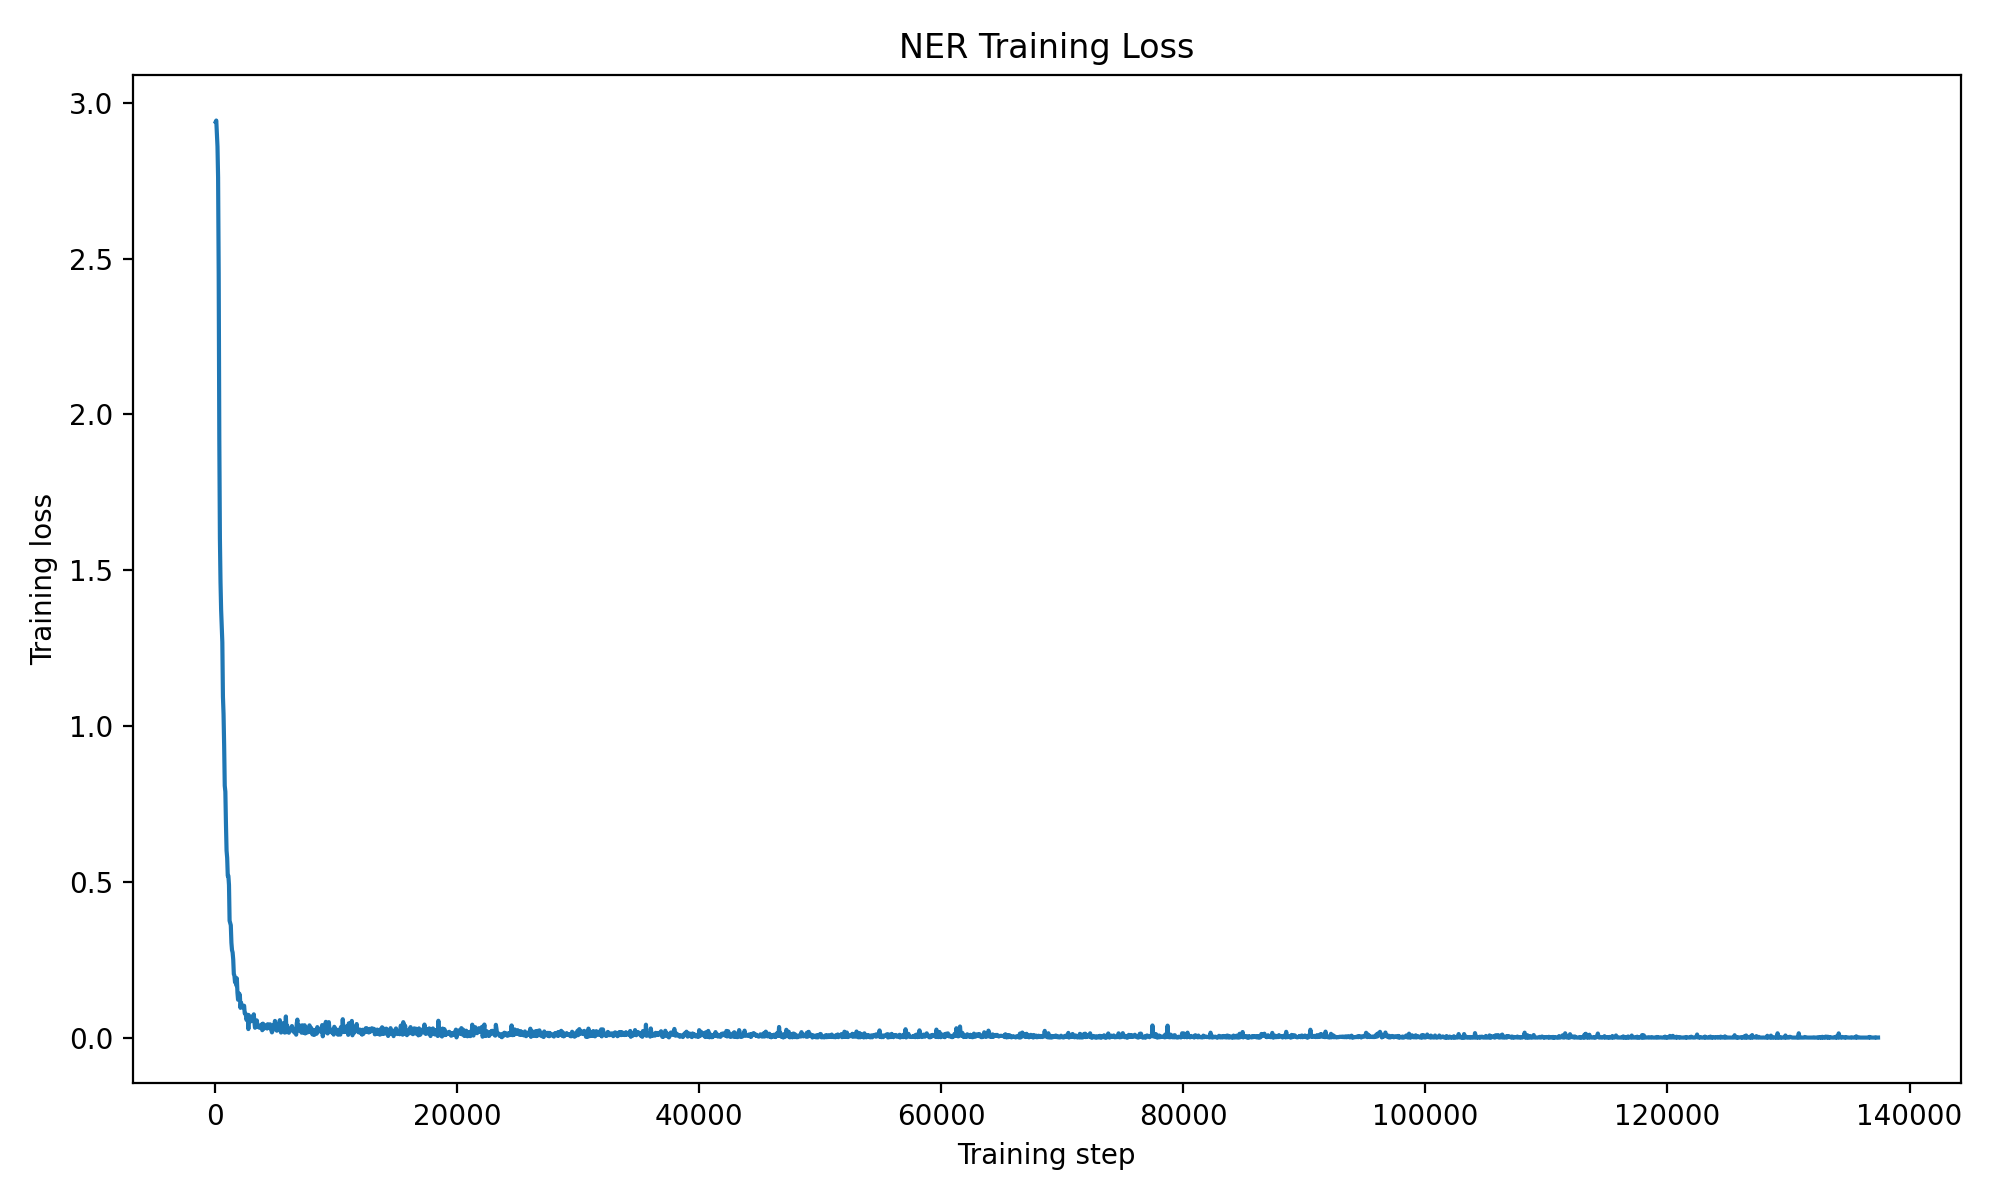
\includegraphics[width=0.82\textwidth]{figures/images/chapter-11/ner/ner_train_loss.png}
\caption{Training loss during fine-tuning of the NER model.}
\label{fig:ner_train_loss}
\end{figure}

\begin{figure}[H]
\centering
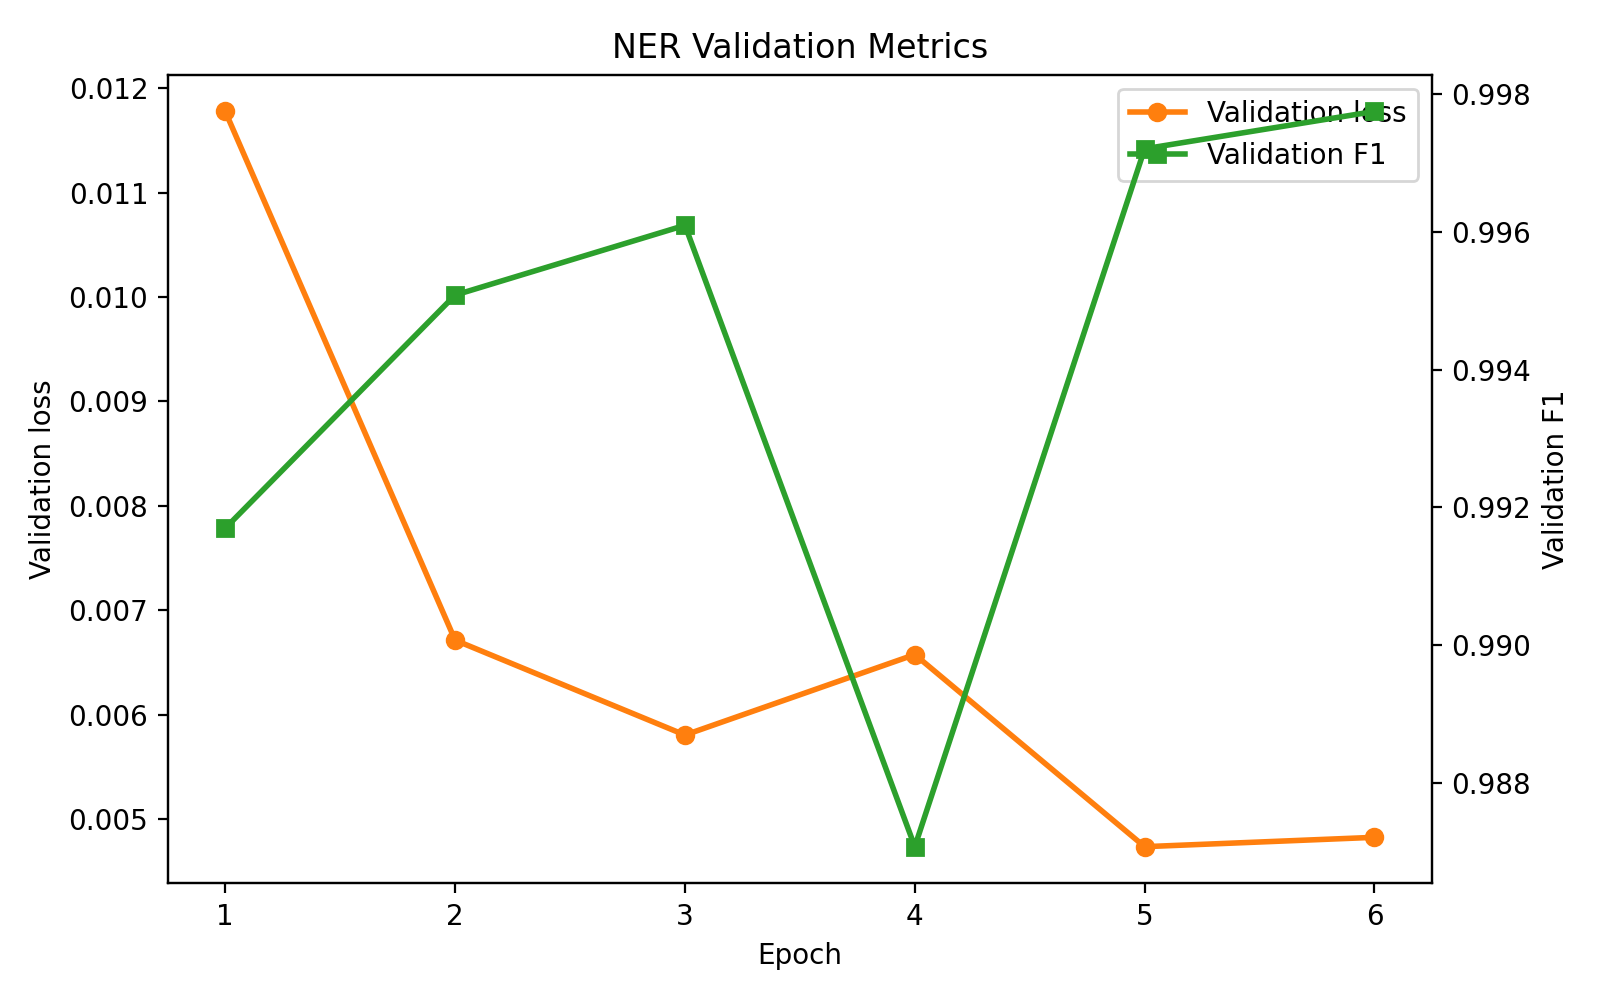
\includegraphics[width=0.78\textwidth]{figures/images/chapter-11/ner/ner_validation_metrics.png}
\caption{Validation loss and validation F1 across training epochs for the NER model. Validation loss is shown on the primary y-axis, while validation F1 is shown on the secondary y-axis.}
\label{fig:ner_validation_metrics}
\end{figure}

Taken together, the curves indicate stable convergence on the constructed training
and validation data, but they do not by themselves demonstrate robust performance
on real-world OCR document scenarios.

\subsection{Per-Label Evaluation}

To better assess generalization, the model was also evaluated on a separate harder
OCR-oriented test set. The overall performance on this set is shown in
Table~\ref{tab:ner_results_hard_appendix}, while the per-label performance is shown
in Table~\ref{tab:ner_hard_test_results} and Figure~\ref{fig:ner_per_label_metrics}.

\begin{table}[H]
\centering
\begin{tabular}{lccc}
\toprule
\textbf{Evaluation set} & \textbf{Precision} & \textbf{Recall} & \textbf{F1 Score} \\
\midrule
Hard test set & 91.32\% & 96.13\% & 0.9366 \\
\bottomrule
\end{tabular}
\caption{Overall NER performance on the harder OCR-oriented test set.}
\label{tab:ner_results_hard_appendix}
\end{table}

\begin{table}[H]
\centering
\begin{tabular}{lcccc}
\toprule
\textbf{Label} & \textbf{Precision} & \textbf{Recall} & \textbf{F1 Score} & \textbf{Support} \\
\midrule
ADDRESS        & 100.00\% & 100.00\% & 1.0000 & 37 \\
DATE           & 100.00\% & 100.00\% & 1.0000 & 50 \\
EMAIL          & 100.00\% & 100.00\% & 1.0000 & 83 \\
ID\_NUMBER     & 90.74\%  & 98.00\%  & 0.9423 & 50 \\
LICENSE\_PLATE & 95.45\%  & 100.00\% & 0.9767 & 21 \\
LOCATION       & 84.21\%  & 88.89\%  & 0.8649 & 72 \\
ORGANIZATION   & 67.16\%  & 95.74\%  & 0.7895 & 47 \\
PERSON\_NAME   & 86.21\%  & 93.75\%  & 0.8982 & 80 \\
PHONE          & 100.00\% & 91.43\%  & 0.9552 & 70 \\
POSTAL\_CODE   & 100.00\% & 100.00\% & 1.0000 & 59 \\
\bottomrule
\end{tabular}
\caption{Per-label performance of the NER model on the harder OCR-oriented test set.}
\label{tab:ner_hard_test_results}
\end{table}

\begin{figure}[H]
\centering
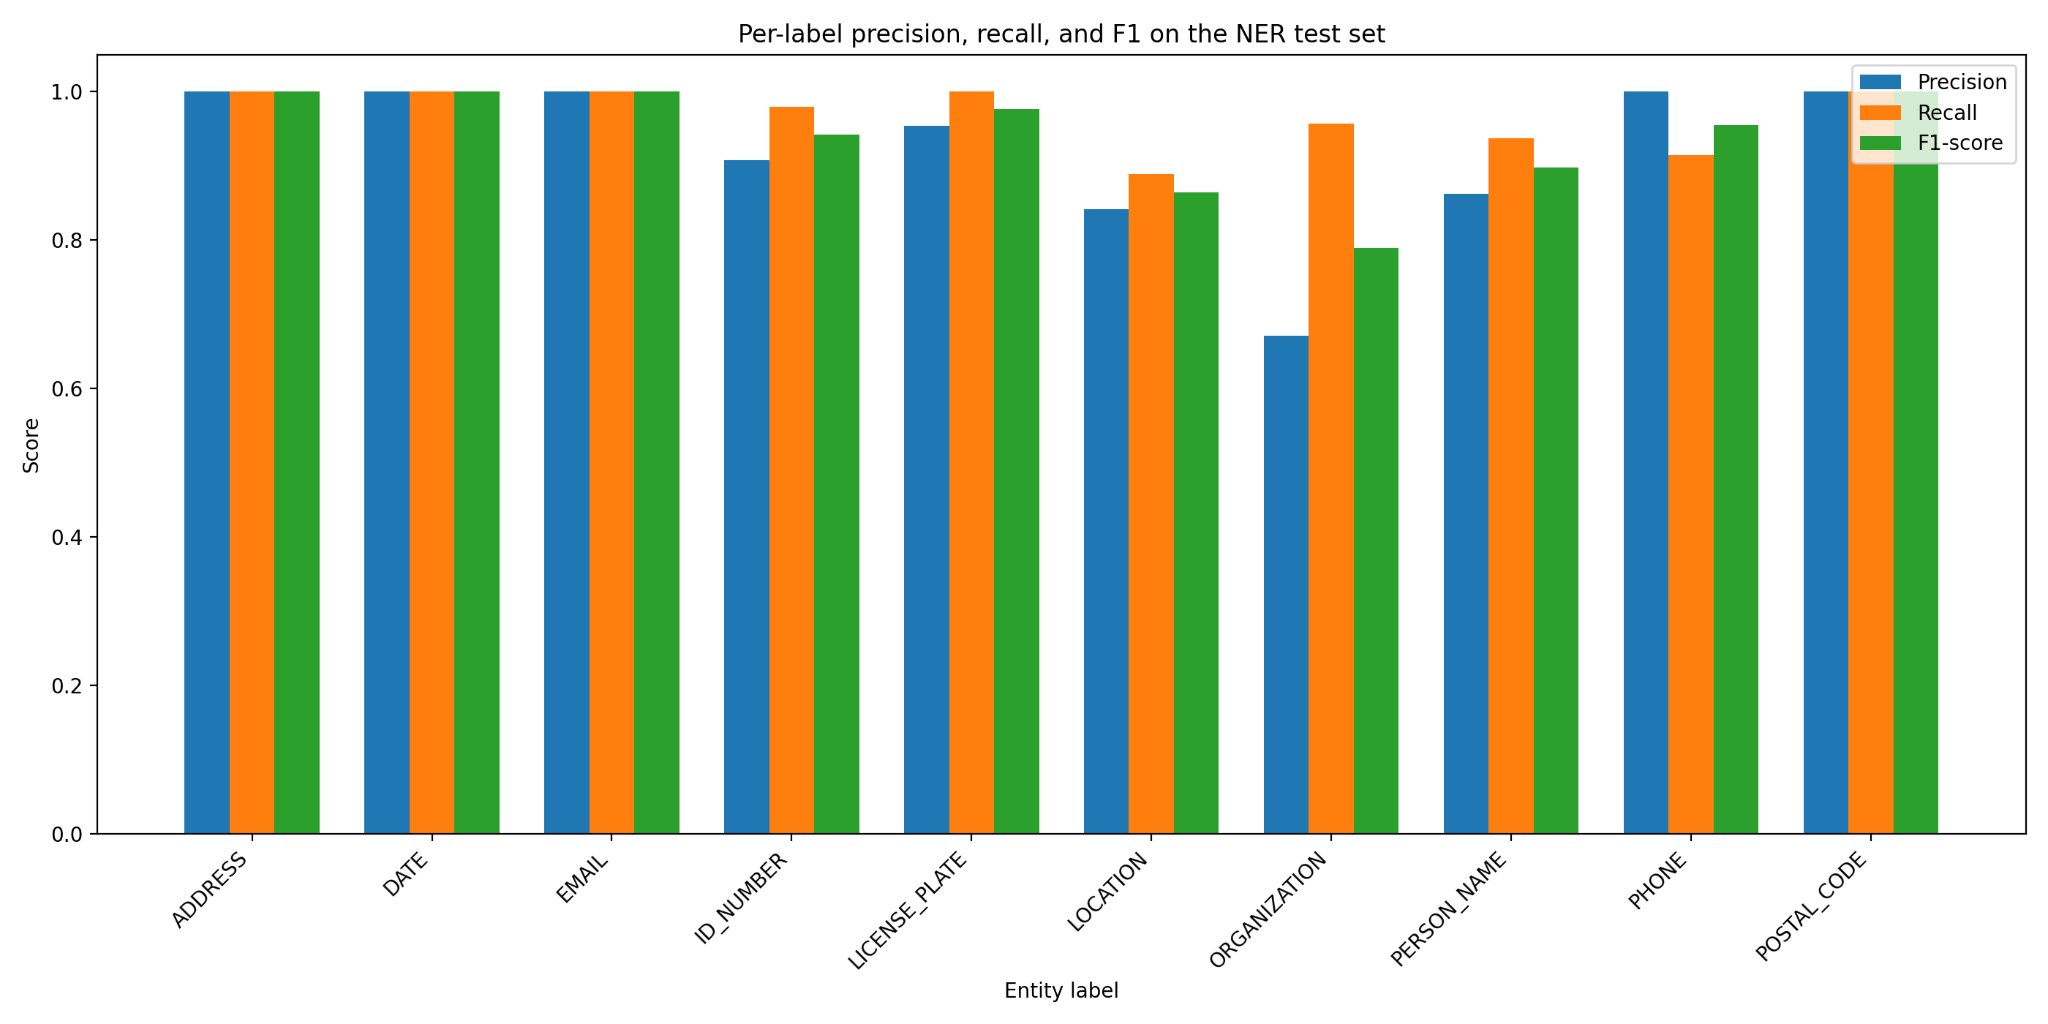
\includegraphics[width=0.9\textwidth]{figures/images/chapter-11/ner/ner_per_label_metrics.png}
\caption{Per-label precision, recall, and F1 on the harder OCR-oriented test set.}
\label{fig:ner_per_label_metrics}
\end{figure}

As shown in Table~\ref{tab:ner_hard_test_results} and
Figure~\ref{fig:ner_per_label_metrics}, the model remained strong on more
structured entity types such as email addresses, postal codes, dates, and
addresses. However, performance was noticeably weaker for semantically more
ambiguous categories such as organizations, locations, and person names. This
indicates that the model generalized less reliably when the OCR text became more
document-oriented and difficult to categorize.

\subsection{Error Analysis}

Figure~\ref{fig:ner_real_vs_controlled } shows a qualitative comparison
between a controlled example and a real-world document scenario. In the
controlled example, the text is more structured and the categorization pipeline
assigns several relevant labels. In the real-world document example, the OCR
text is more fragmented and the assigned categories are less consistent.

These examples illustrate an important limitation of the NER component. While
the model can perform well on structured and simplified inputs, it has greater
difficulty distinguishing reliably between entity categories in practical
document scenarios. This was particularly visible for semantically similar
categories such as person names, organizations, and locations.

\subsection{Summary}

Overall, the NER model achieved very strong results on the constructed held-out
test split and converged stably during training. However, the harder OCR-oriented
evaluation and the qualitative document examples showed that these results
overestimated the practical robustness of the model. In particular, the model
was less reliable for semantically ambiguous categories such as organization,
location, and person-name entities. For this reason, the final SafeVision system
did not rely on the NER model alone, but instead used it as part of a hybrid
text-analysis pipeline.
\chapter{Detailed Video Evaluation Methodology}
\label{app:video_evaluation_details}

This appendix provides additional details and supporting results for the video processing evaluation in Section~\ref{sec:video_processing_results}. Section~\ref{sec:video_processing_results} reports the main system-level results, while this appendix documents the test material, evaluation setup, annotation procedure, metrics, temporal coverage test, and additional failure-case analysis.

\section{Evaluation Setup}

The video evaluation was performed as a system-level extension of the image detection and redaction pipeline. The tests focused on detection frequency, automatic prediction, and manual tracking. They were performed on three short videos with different resolutions, orientations, and durations. Each video was processed using different values of \texttt{detect\_every}, where lower values run detection more frequently and higher values rely more on prediction between detection frames.

\begin{table}[H]
\centering
\begin{tabular}{lcccc}
\toprule
\textbf{Video} & \textbf{Resolution} & \textbf{Frames} & \textbf{Duration} & \textbf{\acrshort{fps}} \\
\midrule
car\_video & $1280\times720$ & 153 & 5.10 s & 30.00 \\
walk & $854\times480$ & 360 & 12.00 s & 30.00 \\
face\_track & $720\times1280$ & 270 & 9.14 s & 29.55 \\
\bottomrule
\end{tabular}
\caption{Overview of videos used for evaluating the video processing pipeline.}
\label{tab:video_test_material}
\end{table}

The evaluation focused on three main aspects. First, automatic Kalman-based prediction was evaluated to determine whether propagated \gls{bounding box}es remained accurate between detection frames. Second, manual tracking was evaluated to determine whether a user-selected object could be followed across a video sequence. Third, processing performance was measured to evaluate how different detection intervals affected runtime.

\section{Ground-Truth Annotation}

Automatic prediction was evaluated by comparing the generated frame-wise manifests with human-labeled ground-truth boxes. The \texttt{detect\_every = 1} configuration was used as a full-detection baseline, but it was excluded from the Kalman prediction accuracy results because no intermediate non-detection frames exist in this configuration. Since every frame receives detector output, the Kalman filter does not need to estimate object positions between detection frames in this case.

For the remaining configurations, predicted boxes were compared with human-labeled boxes on non-detection frames. These frames are important because they represent cases where the system relies on Kalman prediction instead of new detector output.

For manual tracking, the car was first manually annotated on sampled frames across the \texttt{car\_video} video. The manual tracker was then initialized from a ground-truth box in the middle of the video, and the predicted boxes were compared with the human-labeled boxes using \acrshort{iou}.

\section{Evaluation Metrics}

The evaluation used \acrshort{iou} and sensitive-region coverage as the main accuracy metrics.

\paragraph{Intersection over Union}

\acrshort{iou} measures how closely the predicted box aligns with the human-labeled box. It is calculated as the overlap between the predicted and ground-truth boxes divided by their union.

\[
IoU = \frac{Area(B_p \cap B_g)}{Area(B_p \cup B_g)}
\]

where \(B_p\) represents the predicted box and \(B_g\) represents the ground-truth box.

\paragraph{Sensitive-Region Coverage}

Sensitive-region coverage measures how much of the human-labeled sensitive region was covered by the predicted box. This metric was included because anonymization does not only depend on tight localization. A box can be slightly less precise but still cover the sensitive content sufficiently for redaction.

\section{Temporal Coverage Test}

Before evaluating prediction accuracy against human-labeled ground truth, a temporal coverage test was performed. The purpose of this test was not to measure exact tracking accuracy, but to measure whether Kalman-based prediction preserved active \gls{bounding box}es across frames where full detection was not executed.

Since full detection is only executed on selected frames, a detection-only manifest would only contain detected boxes on those frames. Automatic Kalman-based prediction was therefore compared with this detection-frame-only estimate to evaluate whether it preserved the \gls{bounding box}es across non-detection frames.

\begin{table}[H]
\centering
\begin{tabular}{rccc}
\toprule
\textbf{\texttt{detect\_every}} & \textbf{Detection calls} & \textbf{Detection-only} & \textbf{Manifest with prediction} \\
\midrule
1  & 261.00 & 99.44\% & 99.44\% \\
2  & 130.67 & 50.02\% & 99.63\% \\
5  & 52.33  & 20.09\% & 99.63\% \\
10 & 26.33  & 10.15\% & 99.17\% \\
\bottomrule
\end{tabular}
\caption{Average frame coverage across the three tested videos. ``Detection-only'' estimates the percentage of frames that would contain boxes if boxes were only used on frames where full detection was executed. ``Manifest with prediction'' shows the percentage of frames with active boxes after Kalman-based prediction has propagated boxes between detection frames.}
\label{tab:video_temporal_coverage}
\end{table}

Kalman-based prediction substantially increased bounding-box coverage when detection was run less frequently. With \texttt{detect\_every = 10}, the detection-frame estimate was 10.15\%, while the prediction-based manifest maintained 99.17\% coverage on average. This confirms that the prediction step filled the gaps between detection frames and produced continuous boxes for later review and redaction.

However, this metric should be interpreted only as a temporal coverage result. It shows whether boxes were present in the frame-wise manifest, but it does not show whether the boxes were accurately aligned with the sensitive objects. For this reason, the main video evaluation in Section~\ref{sec:video_processing_results} uses human-labeled ground truth, \acrshort{iou}, and sensitive-region coverage as the primary accuracy results.

\section{Processing-Time Benchmark Setup}

Processing performance was evaluated using the same \texttt{detect\_every} values as the prediction accuracy evaluation. Each configuration was run three times after a warmup run, and the reported values were averaged across the three tested videos. The benchmark was executed on CPU.

The measured processing time included the complete video processing path used in the evaluation, including frame decoding, selected frame-level detection calls, prediction between detection frames, and manifest generation. The purpose of the benchmark was to measure how reducing the number of detection calls affected total processing cost.

\section{Worst-Frame Example}

Figure~\ref{fig:video_prediction_worst_frame} shows the lowest-quality frame found in the \texttt{car\_video} sequence when using \texttt{detect\_every = 10}. This example was selected from the human-labeled evaluation and illustrates a difficult case with several nearby moving vehicles.

\begin{figure}[H]
\centering
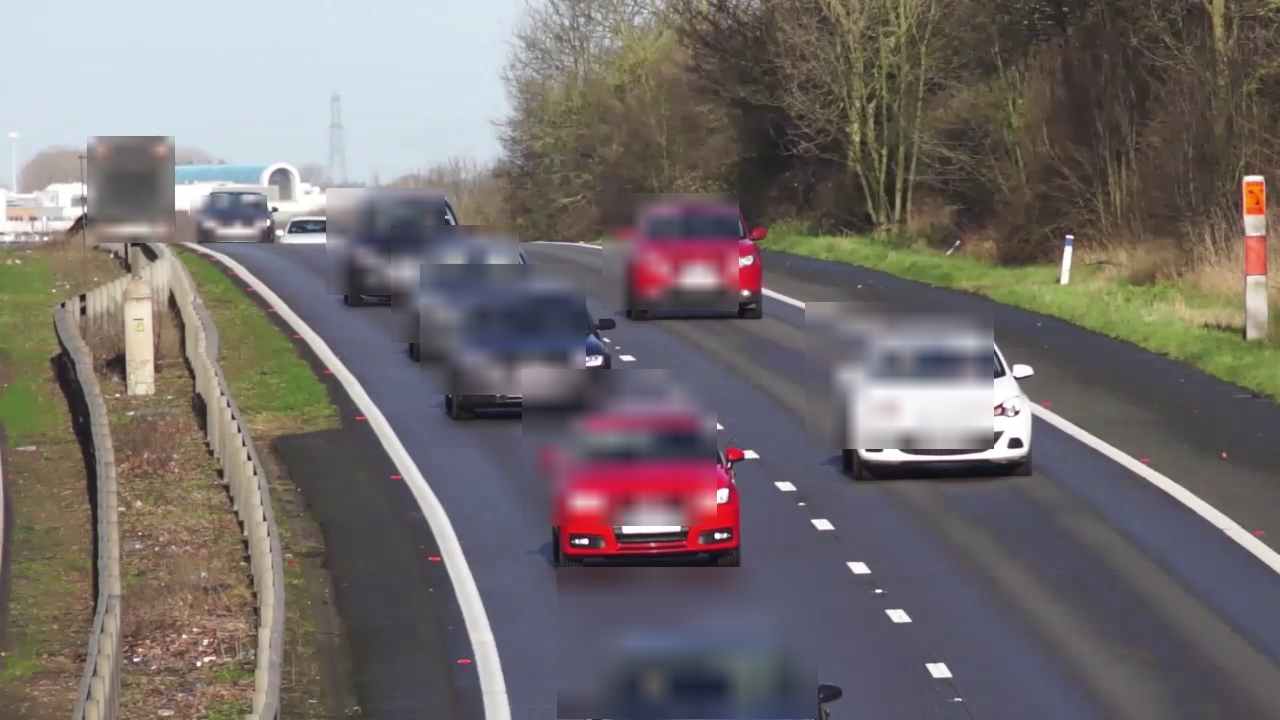
\includegraphics[width=0.85\textwidth]{figures/images/chapter-11/car_kalman_worst_frame.png}
\caption{Worst-frame example from the \texttt{car\_video} sequence using \texttt{detect\_every = 10}. The frame contained nine human-labeled vehicle boxes and ten predicted boxes. The mean \acrshort{iou} was 0.5245, while mean sensitive-region coverage was 0.7469. This illustrates that long prediction intervals can reduce localization accuracy in frames with several nearby moving objects.}
\label{fig:video_prediction_worst_frame}
\end{figure}

This example shows why both \acrshort{iou} and sensitive-region coverage were used in the main evaluation. The predicted boxes still cover large parts of the sensitive regions, but the alignment is less precise than in easier frames. This makes the frame useful as a qualitative example of the limitations of longer prediction intervals.

The lower \acrshort{iou} in this frame was mainly caused by several nearby moving vehicles that produced overlapping prediction paths between sparse detection frames. This type of scenario is more challenging for prediction than isolated objects with stable movement. The example supports the main result that \texttt{detect\_every = 10} provides the largest runtime reduction, but also increases the risk of localization drift in crowded or fast-moving scenes.
\chapter{Training Configuration Details}
\label{app:yolox_config}

\section{QR and Barcode Detection Model}

\begin{lstlisting}[caption={YOLOX experiment file for QR and barcode detection}, label={lst:yolox_barcode}]
"""
YOLOX experiment configuration for QR and barcode detection.

This configuration defines the training setup used for the custom
barcode detection model. The model is based on the YOLOX-S architecture
and trained on a merged dataset containing both real and synthetic data.

The configuration includes dataset paths, training parameters, and
augmentation settings used during training.
"""

from yolox.exp import Exp as MyExp
from yolox.data import COCODataset, TrainTransform, ValTransform
import os


class Exp(MyExp):
    def __init__(self):
        super(Exp, self).__init__()

        # Experiment name
        self.exp_name = "barcode_merged_yolox_s"

        # --------------------------------------------------
        # Model configuration (YOLOX-S)
        # --------------------------------------------------
        self.depth = 0.33
        self.width = 0.50
        self.num_classes = 1  # Single class: barcode / QR / visual code

        # --------------------------------------------------
        # Dataset configuration
        # --------------------------------------------------
        self.data_dir = os.path.abspath(
            os.path.join(os.path.dirname(__file__), "../../../../barcodeV2/dataset_merged")
        )

        # Annotation files (COCO format)
        self.train_ann = "instances_train2017.json"
        self.val_ann = "instances_test2017.json"  # Used for evaluation

        # Image directories
        self.train_name = "train2017"
        self.val_name = "test2017"

        # --------------------------------------------------
        # Training configuration
        # --------------------------------------------------
        self.max_epoch = 200
        self.data_num_workers = 4

        # Higher resolution improves detection of small barcodes
        # but increases GPU memory usage
        self.input_size = (960, 960)
        self.test_size = (960, 960)

        self.print_interval = 20
        self.eval_interval = 1

        # --------------------------------------------------
        # Data augmentation configuration
        # --------------------------------------------------
        # Mosaic and MixUp disabled due to already diverse dataset
        self.mosaic_prob = 0.0
        self.mixup_prob = 0.0

        # Moderate online augmentations
        self.hsv_prob = 0.5        # Color jitter
        self.flip_prob = 0.5       # Horizontal flip

        # Geometric transformations (kept small to preserve structure)
        self.degrees = 5.0
        self.translate = 0.05
        self.shear = 1.0

    def get_dataset(self, cache=False, cache_type=None):
        """
        Returns the training dataset using COCO format.
        """
        return COCODataset(
            data_dir=self.data_dir,
            json_file=self.train_ann,
            name=self.train_name,
            img_size=self.input_size,
            preproc=TrainTransform(
                max_labels=120,
                flip_prob=self.flip_prob,
                hsv_prob=self.hsv_prob,
            ),
            cache=cache,
            cache_type=cache_type,
        )

    def get_eval_dataset(self, testdev=False, legacy=False, **kwargs):
        """
        Returns the evaluation dataset.
        """
        return COCODataset(
            data_dir=self.data_dir,
            json_file=self.val_ann,
            name=self.val_name,
            img_size=self.test_size,
            preproc=ValTransform(legacy=legacy),
        )
\end{lstlisting}

\section{License Plate Detection Model}

\begin{lstlisting}[caption={YOLOX experiment file for license plate detection}, label={lst:yolox_licenseplate}]
"""
YOLOX experiment configuration for license plate detection.

This configuration defines the training and evaluation setup for the
license plate detection model. The model is based on YOLOX-S and trained
on a custom dataset with COCO-style annotations.

Compared to the barcode model, this configuration uses more aggressive
data augmentation (e.g., mosaic) to improve generalization.
"""

#!/usr/bin/env python3
# -*- coding:utf-8 -*-

import os
import torch
from yolox.exp import Exp as MyExp
from yolox.data import COCODataset, ValTransform
from yolox.evaluators import COCOEvaluator


class Exp(MyExp):
    def __init__(self):
        super().__init__()

        # Experiment name
        self.exp_name = "yolox_s_license_plate"

        # --------------------------------------------------
        # Model configuration (YOLOX-S)
        # --------------------------------------------------
        self.depth = 0.33
        self.width = 0.50
        self.num_classes = 1  # Single class: license plate

        # --------------------------------------------------
        # Dataset configuration
        # --------------------------------------------------
        self.data_dir = os.path.abspath(
            os.path.join(os.path.dirname(__file__), "../../../../license_plate_detection/dataset")
        )

        self.train_ann = "train.json"
        self.val_ann = "test.json"  # Used only for evaluation

        # --------------------------------------------------
        # Training configuration
        # --------------------------------------------------
        self.input_size = (960, 960)
        self.test_size = (960, 960)

        self.max_epoch = 200
        self.no_aug_epochs = 15

        # Learning rate schedule
        self.basic_lr_per_img = 0.01 / 64.0
        self.min_lr_ratio = 0.05
        self.warmup_epochs = 5

        self.data_num_workers = 2
        self.print_interval = 20
        self.eval_interval = 1

        # --------------------------------------------------
        # Data augmentation configuration
        # --------------------------------------------------
        # Mosaic enabled to improve generalization
        self.mosaic_scale = (0.5, 1.5)
        self.mosaic_prob = 0.8

        # MixUp disabled
        self.mixup_prob = 0.0
        self.enable_mixup = False

        # Standard augmentations
        self.hsv_prob = 0.5
        self.flip_prob = 0.5

        # Geometric transformations
        self.degrees = 5.0
        self.translate = 0.05
        self.shear = 1.0

        # Multi-scale training
        self.random_size = (14, 24)

        # --------------------------------------------------
        # Evaluation settings
        # --------------------------------------------------
        self.test_conf = 0.01
        self.nmsthre = 0.65

        self.output_dir = "./YOLOX_outputs"

    def get_eval_loader(self, batch_size, is_distributed, testdev=False, legacy=False):
        """
        Creates the evaluation data loader.
        """
        image_folder = "test2017" if self.val_ann == "test.json" else "val2017"

        valdataset = COCODataset(
            data_dir=self.data_dir,
            json_file=self.val_ann,
            name=image_folder,
            img_size=self.test_size,
            preproc=ValTransform(legacy=legacy),
        )

        if is_distributed:
            batch_size = batch_size // torch.distributed.get_world_size()
            sampler = torch.utils.data.distributed.DistributedSampler(
                valdataset, shuffle=False
            )
        else:
            sampler = torch.utils.data.SequentialSampler(valdataset)

        return torch.utils.data.DataLoader(
            valdataset,
            batch_size=batch_size,
            sampler=sampler,
            num_workers=self.data_num_workers,
            pin_memory=True,
        )

    def get_evaluator(self, batch_size, is_distributed, testdev=False, legacy=False):
        """
        Returns the COCO evaluator used for model evaluation.
        """
        return COCOEvaluator(
            dataloader=self.get_eval_loader(batch_size, is_distributed, testdev, legacy),
            img_size=self.test_size,
            confthre=self.test_conf,
            nmsthre=self.nmsthre,
            num_classes=self.num_classes,
            testdev=testdev,
        )
\end{lstlisting}
\chapter{Hybrid Text Analysis Pipeline}
\label{app:pii_detector}

In the deployed system, OCR-extracted text was not classified by the NER model
alone. Instead, the final text categorization step was implemented through a
hybrid pipeline in \texttt{pii\_detector.py}, where NER predictions were
combined with rule-based checks, contextual field hints, and post-processing
filters. Listings~\ref{lst:pii_detector_extract} and
\ref{lst:pii_detector_rules} show the central extraction logic and an example of
the rule-based entity detection used in the final system.

\begin{lstlisting}[language=Python, caption={Core hybrid extraction logic used after OCR text recognition}, label={lst:pii_detector_extract}]
def extract_entities(
    text: str,
    expected_label: Optional[str] = None,
) -> List[TextEntity]:
    clean = normalize_text(text)
    if not clean:
        return []

    all_rule_ents: List[TextEntity] = []
    all_gliner_ents: List[TextEntity] = []
    all_custom_ents: List[TextEntity] = []

    all_rule_ents.extend(detect_rule_entities(clean, expected_label))
    all_custom_ents.extend(detect_custom_ner_entities(clean, expected_label))
    all_gliner_ents.extend(detect_gliner_entities(clean, expected_label))

    for line in split_lines(clean):
        key, value = extract_key_value(line)
        line_expected = context_label_from_key(key) or expected_label
        segment = value if key else line

        if not segment or is_noise(segment):
            continue

        all_rule_ents.extend(detect_rule_entities(segment, line_expected))
        all_custom_ents.extend(detect_custom_ner_entities(segment, line_expected))
        all_gliner_ents.extend(detect_gliner_entities(segment, line_expected))

        # ... context-based helper rules omitted ...

    entities = merge_all(all_rule_ents, all_gliner_ents, all_custom_ents)

    if (
        not entities
        and expected_label in {"POSTAL_CODE", "PHONE", "ID_NUMBER", "DATE"}
        and len(clean) >= 2
        and not is_noise(clean)
    ):
        entities = [TextEntity(clean, expected_label, 0.50, "context")]

    return dedupe_entities(entities)
\end{lstlisting}

\begin{lstlisting}[language=Python, caption={Example of rule-based entity detection used alongside NER}, label={lst:pii_detector_rules}]
def detect_rule_entities(
    text: str,
    expected_label: Optional[str] = None,
) -> List[TextEntity]:
    t = normalize_token(text)
    entities: List[TextEntity] = []

    if is_noise(t):
        return entities

    for m in EMAIL_RE.finditer(t):
        entities.append(TextEntity(m.group(0), "EMAIL", 0.99, "regex"))

    if NOR_PHONE_RE.fullmatch(t) and is_valid_phone(t):
        entities.append(TextEntity(t, "PHONE", 0.97, "rule"))
    elif expected_label == "PHONE":
        for m in GENERIC_PHONE_RE.finditer(t):
            if is_valid_phone(m.group(0)):
                entities.append(TextEntity(m.group(0), "PHONE", 0.90, "regex+context"))

    if POSTAL_RE.fullmatch(t):
        entities.append(TextEntity(t, "POSTAL_CODE", 0.96, "rule"))

    if looks_like_date(t):
        entities.append(TextEntity(t, "DATE", 0.93, "rule"))

    # ... additional rules omitted ...

    return dedupe_entities(entities)
\end{lstlisting}

Listing~\ref{lst:pii_detector_extract} shows that the final text-analysis
component combined multiple sources of evidence rather than relying only on the
NER model. Listing~\ref{lst:pii_detector_rules} illustrates how structured
entity types such as email addresses, phone numbers, postal codes, and dates
were reinforced through explicit rules in addition to model-based predictions.
\chapter{Detailed Test Coverage}
\label{app:test_cov_detailed}


\section{Frontend Coverage Report}
\label{appendix:frontend_coverage_full}

% Auto-generated from coverage/coverage-final.json
\footnotesize
\begin{longtable}{>{\raggedright\arraybackslash}p{0.72\textwidth}rrr}
\hline
\textbf{File} & \textbf{Stmts} & \textbf{Miss} & \textbf{Cover} \\
\hline
\endfirsthead
\hline
\textbf{File} & \textbf{Stmts} & \textbf{Miss} & \textbf{Cover} \\
\hline
\endhead
src/\allowbreak App.tsx & 5 & 0 & 100.00\% \\
src/\allowbreak app/\allowbreak AppShell.tsx & 19 & 15 & 21.05\% \\
src/\allowbreak app/\allowbreak useAppController.ts & 36 & 4 & 88.89\% \\
src/\allowbreak features/\allowbreak detection/\allowbreak components/\allowbreak CategoryMultiSelect.tsx & 45 & 27 & 40.00\% \\
src/\allowbreak features/\allowbreak detection/\allowbreak components/\allowbreak DetectionFiltersSection.tsx & 26 & 8 & 69.23\% \\
src/\allowbreak features/\allowbreak detection/\allowbreak domain/\allowbreak detectionFilters.logic.ts & 25 & 18 & 28.00\% \\
src/\allowbreak features/\allowbreak detection/\allowbreak domain/\allowbreak detectionGroups.ts & 2 & 0 & 100.00\% \\
src/\allowbreak features/\allowbreak detection/\allowbreak domain/\allowbreak detectionMapping.ts & 7 & 3 & 57.14\% \\
src/\allowbreak features/\allowbreak detection/\allowbreak domain/\allowbreak detectionSelection.logic.ts & 14 & 5 & 64.29\% \\
src/\allowbreak features/\allowbreak detection/\allowbreak hooks/\allowbreak useDetectionFilters.ts & 2 & 1 & 50.00\% \\
src/\allowbreak features/\allowbreak detection/\allowbreak state/\allowbreak detectionFiltersStore.ts & 31 & 2 & 93.55\% \\
src/\allowbreak features/\allowbreak file/\allowbreak component/\allowbreak FilePanel.tsx & 52 & 44 & 15.38\% \\
src/\allowbreak features/\allowbreak file/\allowbreak component/\allowbreak Sidebar.tsx & 32 & 21 & 34.38\% \\
src/\allowbreak features/\allowbreak file/\allowbreak context/\allowbreak FileTaskProgressContext.tsx & 2 & 0 & 100.00\% \\
src/\allowbreak features/\allowbreak file/\allowbreak context/\allowbreak FileTaskProgressContextValue.ts & 1 & 0 & 100.00\% \\
src/\allowbreak features/\allowbreak file/\allowbreak context/\allowbreak FileTaskProgressTypes.ts & 0 & 0 & 100.00\% \\
src/\allowbreak features/\allowbreak file/\allowbreak hooks/\allowbreak useFileActions.ts & 77 & 20 & 74.03\% \\
src/\allowbreak features/\allowbreak file/\allowbreak hooks/\allowbreak useFileDelete.ts & 11 & 9 & 18.18\% \\
src/\allowbreak features/\allowbreak file/\allowbreak hooks/\allowbreak useFileSelection.ts & 74 & 27 & 63.51\% \\
src/\allowbreak features/\allowbreak file/\allowbreak hooks/\allowbreak useFileTaskProgress.ts & 2 & 0 & 100.00\% \\
src/\allowbreak features/\allowbreak file/\allowbreak hooks/\allowbreak useFileUpload.ts & 19 & 17 & 10.53\% \\
src/\allowbreak features/\allowbreak file/\allowbreak hooks/\allowbreak useHistoryAwareStores.ts & 44 & 13 & 70.45\% \\
src/\allowbreak features/\allowbreak file/\allowbreak hooks/\allowbreak useTaskProgressManagement.ts & 20 & 11 & 45.00\% \\
src/\allowbreak features/\allowbreak file/\allowbreak model/\allowbreak fileClipboard.ts & 32 & 5 & 84.38\% \\
src/\allowbreak features/\allowbreak file/\allowbreak model/\allowbreak reorderImages.ts & 18 & 16 & 11.11\% \\
src/\allowbreak features/\allowbreak highlights/\allowbreak components/\allowbreak HighlightColorChip.tsx & 3 & 3 & 0.00\% \\
src/\allowbreak features/\allowbreak userPreference/\allowbreak components/\allowbreak StylesPanel.tsx & 49 & 25 & 48.98\% \\
src/\allowbreak features/\allowbreak userPreference/\allowbreak components/\allowbreak UserPreferencePanel.tsx & 2 & 0 & 100.00\% \\
src/\allowbreak features/\allowbreak userPreference/\allowbreak context/\allowbreak UserPreferencesContext.ts & 1 & 0 & 100.00\% \\
src/\allowbreak features/\allowbreak userPreference/\allowbreak context/\allowbreak UserPreferencesProvider.tsx & 5 & 0 & 100.00\% \\
src/\allowbreak features/\allowbreak userPreference/\allowbreak context/\allowbreak UserPreferencesTypes.ts & 0 & 0 & 100.00\% \\
src/\allowbreak features/\allowbreak userPreference/\allowbreak hooks/\allowbreak useApplyTheme.ts & 33 & 19 & 42.42\% \\
src/\allowbreak features/\allowbreak userPreference/\allowbreak hooks/\allowbreak useEditorShortcuts.ts & 18 & 15 & 16.67\% \\
src/\allowbreak features/\allowbreak userPreference/\allowbreak hooks/\allowbreak useGlobalShortcuts.ts & 35 & 25 & 28.57\% \\
src/\allowbreak features/\allowbreak userPreference/\allowbreak hooks/\allowbreak useTaskProgress.ts & 32 & 4 & 87.50\% \\
src/\allowbreak features/\allowbreak userPreference/\allowbreak hooks/\allowbreak useUserPreferences.ts & 4 & 1 & 75.00\% \\
src/\allowbreak features/\allowbreak userPreference/\allowbreak hooks/\allowbreak useUserPreferencesState.ts & 52 & 27 & 48.08\% \\
src/\allowbreak features/\allowbreak userPreference/\allowbreak index.ts & 0 & 0 & 100.00\% \\
src/\allowbreak features/\allowbreak userPreference/\allowbreak model/\allowbreak userPreferences.ts & 1 & 0 & 100.00\% \\
src/\allowbreak features/\allowbreak userPreference/\allowbreak utils/\allowbreak highlightStyle.ts & 9 & 0 & 100.00\% \\
src/\allowbreak features/\allowbreak userPreference/\allowbreak utils/\allowbreak shortcut.ts & 36 & 3 & 91.67\% \\
src/\allowbreak features/\allowbreak workspace/\allowbreak components/\allowbreak ContextMenu.tsx & 11 & 4 & 63.64\% \\
src/\allowbreak features/\allowbreak workspace/\allowbreak components/\allowbreak DragOverlay.tsx & 3 & 1 & 66.67\% \\
src/\allowbreak features/\allowbreak workspace/\allowbreak components/\allowbreak WorkspaceEmptyState.tsx & 1 & 0 & 100.00\% \\
src/\allowbreak features/\allowbreak workspace/\allowbreak hooks/\allowbreak state/\allowbreak useWorkspaceAIMission.ts & 13 & 10 & 23.08\% \\
src/\allowbreak features/\allowbreak workspace/\allowbreak hooks/\allowbreak state/\allowbreak useWorkspaceRedaction.ts & 115 & 102 & 11.30\% \\
src/\allowbreak features/\allowbreak workspace/\allowbreak hooks/\allowbreak useCanvasHover.ts & 15 & 11 & 26.67\% \\
src/\allowbreak features/\allowbreak workspace/\allowbreak hooks/\allowbreak useHighlightBoxEditor.ts & 125 & 108 & 13.60\% \\
src/\allowbreak features/\allowbreak workspace/\allowbreak hooks/\allowbreak useVisibleHighlights.ts & 2 & 0 & 100.00\% \\
src/\allowbreak features/\allowbreak workspace/\allowbreak hooks/\allowbreak useWorkspaceFileDrop.ts & 36 & 2 & 94.44\% \\
src/\allowbreak features/\allowbreak workspace/\allowbreak media/\allowbreak image/\allowbreak ImageWorkspace.tsx & 135 & 106 & 21.48\% \\
src/\allowbreak features/\allowbreak workspace/\allowbreak media/\allowbreak image/\allowbreak components/\allowbreak CanvasSurface.tsx & 72 & 72 & 0.00\% \\
src/\allowbreak features/\allowbreak workspace/\allowbreak media/\allowbreak image/\allowbreak components/\allowbreak PageEditorSurface.tsx & 55 & 28 & 49.09\% \\
src/\allowbreak features/\allowbreak workspace/\allowbreak media/\allowbreak image/\allowbreak hooks/\allowbreak boxClipboard.ts & 6 & 1 & 83.33\% \\
src/\allowbreak features/\allowbreak workspace/\allowbreak media/\allowbreak image/\allowbreak hooks/\allowbreak useCanvasImage.ts & 32 & 32 & 0.00\% \\
src/\allowbreak features/\allowbreak workspace/\allowbreak media/\allowbreak image/\allowbreak hooks/\allowbreak useImageAIMission.ts & 91 & 35 & 61.54\% \\
src/\allowbreak features/\allowbreak workspace/\allowbreak media/\allowbreak image/\allowbreak hooks/\allowbreak useImageBoxes.ts & 56 & 37 & 33.93\% \\
src/\allowbreak features/\allowbreak workspace/\allowbreak media/\allowbreak image/\allowbreak hooks/\allowbreak useImageEditor.ts & 14 & 14 & 0.00\% \\
src/\allowbreak features/\allowbreak workspace/\allowbreak media/\allowbreak image/\allowbreak hooks/\allowbreak useImageRedaction.ts & 53 & 53 & 0.00\% \\
src/\allowbreak features/\allowbreak workspace/\allowbreak media/\allowbreak video/\allowbreak VideoCanvasOverlay.tsx & 229 & 155 & 32.31\% \\
src/\allowbreak features/\allowbreak workspace/\allowbreak media/\allowbreak video/\allowbreak VideoWorkspace.tsx & 101 & 100 & 0.99\% \\
src/\allowbreak features/\allowbreak workspace/\allowbreak media/\allowbreak video/\allowbreak hooks/\allowbreak useVideoAIMission.ts & 43 & 43 & 0.00\% \\
src/\allowbreak features/\allowbreak workspace/\allowbreak media/\allowbreak video/\allowbreak hooks/\allowbreak useVideoObjectUrls.ts & 26 & 26 & 0.00\% \\
src/\allowbreak features/\allowbreak workspace/\allowbreak media/\allowbreak video/\allowbreak hooks/\allowbreak useVideoPlaybackState.ts & 179 & 24 & 86.59\% \\
src/\allowbreak features/\allowbreak workspace/\allowbreak media/\allowbreak video/\allowbreak hooks/\allowbreak useVideoRedaction.ts & 37 & 37 & 0.00\% \\
src/\allowbreak features/\allowbreak workspace/\allowbreak media/\allowbreak video/\allowbreak utils/\allowbreak videoDetectionOptions.ts & 46 & 1 & 97.83\% \\
src/\allowbreak features/\allowbreak workspace/\allowbreak media/\allowbreak video/\allowbreak utils/\allowbreak videoManifest.ts & 77 & 18 & 76.62\% \\
src/\allowbreak features/\allowbreak workspace/\allowbreak utils/\allowbreak \_\_testUtils\_\_/\allowbreak rect.ts & 1 & 0 & 100.00\% \\
src/\allowbreak features/\allowbreak workspace/\allowbreak utils/\allowbreak canvasExporter.ts & 84 & 63 & 25.00\% \\
src/\allowbreak features/\allowbreak workspace/\allowbreak utils/\allowbreak detectionLabel.ts & 23 & 9 & 60.87\% \\
src/\allowbreak features/\allowbreak workspace/\allowbreak utils/\allowbreak rectHitTest.ts & 45 & 9 & 80.00\% \\
src/\allowbreak features/\allowbreak workspace/\allowbreak utils/\allowbreak rectTransform.ts & 13 & 0 & 100.00\% \\
src/\allowbreak features/\allowbreak workspace/\allowbreak utils/\allowbreak workspaceHandle.ts & 0 & 0 & 100.00\% \\
src/\allowbreak hooks/\allowbreak effects/\allowbreak useAIMissionProgress.ts & 42 & 10 & 76.19\% \\
src/\allowbreak hooks/\allowbreak state/\allowbreak useDetectionsStore.ts & 23 & 0 & 100.00\% \\
src/\allowbreak hooks/\allowbreak state/\allowbreak useEditorHistory.ts & 27 & 0 & 100.00\% \\
src/\allowbreak hooks/\allowbreak state/\allowbreak useHighlightsForImage.ts & 27 & 27 & 0.00\% \\
src/\allowbreak hooks/\allowbreak state/\allowbreak useHighlightsStore.ts & 57 & 2 & 96.49\% \\
src/\allowbreak hooks/\allowbreak state/\allowbreak useImages.ts & 32 & 0 & 100.00\% \\
src/\allowbreak hooks/\allowbreak state/\allowbreak useUndoRedoHistory.ts & 78 & 7 & 91.03\% \\
src/\allowbreak hooks/\allowbreak state/\allowbreak useVideoManifestStore.ts & 62 & 16 & 74.19\% \\
src/\allowbreak hooks/\allowbreak ui/\allowbreak useCloseOnEscapeAndOutsideClick.ts & 19 & 1 & 94.74\% \\
src/\allowbreak hooks/\allowbreak ui/\allowbreak useConsentGate.ts & 52 & 7 & 86.54\% \\
src/\allowbreak hooks/\allowbreak ui/\allowbreak useContextMenu.ts & 20 & 6 & 70.00\% \\
src/\allowbreak hooks/\allowbreak ui/\allowbreak useCtrlDragPan.ts & 47 & 25 & 46.81\% \\
src/\allowbreak hooks/\allowbreak ui/\allowbreak useMediaQuery.ts & 15 & 2 & 86.67\% \\
src/\allowbreak hooks/\allowbreak ui/\allowbreak usePreventBrowserZoom.ts & 14 & 1 & 92.86\% \\
src/\allowbreak hooks/\allowbreak ui/\allowbreak useSidebarState.ts & 15 & 3 & 80.00\% \\
src/\allowbreak hooks/\allowbreak ui/\allowbreak useTopbarFit.ts & 34 & 20 & 41.18\% \\
src/\allowbreak hooks/\allowbreak ui/\allowbreak useVideoFullscreenProxy.ts & 64 & 7 & 89.06\% \\
src/\allowbreak hooks/\allowbreak ui/\allowbreak useViewportWheelZoom.ts & 30 & 22 & 26.67\% \\
src/\allowbreak hooks/\allowbreak ui/\allowbreak useZoom.ts & 16 & 0 & 100.00\% \\
src/\allowbreak lib/\allowbreak canvas/\allowbreak canvasDraw.ts & 55 & 54 & 1.82\% \\
src/\allowbreak main.tsx & 1 & 1 & 0.00\% \\
src/\allowbreak models/\allowbreak detectionCategories.ts & 10 & 0 & 100.00\% \\
src/\allowbreak models/\allowbreak detectionFilters.ts & 35 & 8 & 77.14\% \\
src/\allowbreak models/\allowbreak image.ts & 0 & 0 & 100.00\% \\
src/\allowbreak models/\allowbreak imageDocumentId.ts & 5 & 5 & 0.00\% \\
src/\allowbreak models/\allowbreak imageInstance.ts & 12 & 12 & 0.00\% \\
src/\allowbreak models/\allowbreak rect.ts & 0 & 0 & 100.00\% \\
src/\allowbreak models/\allowbreak redaction.ts & 0 & 0 & 100.00\% \\
src/\allowbreak services/\allowbreak detection/\allowbreak detectionApi.ts & 17 & 17 & 0.00\% \\
src/\allowbreak services/\allowbreak http/\allowbreak abortError.ts & 3 & 3 & 0.00\% \\
src/\allowbreak services/\allowbreak http/\allowbreak apiClient.ts & 1 & 0 & 100.00\% \\
src/\allowbreak services/\allowbreak http/\allowbreak httpClient.ts & 26 & 26 & 0.00\% \\
src/\allowbreak services/\allowbreak redaction/\allowbreak redactionApi.ts & 14 & 14 & 0.00\% \\
src/\allowbreak services/\allowbreak storage/\allowbreak browserStorageKeys.ts & 38 & 8 & 78.95\% \\
src/\allowbreak services/\allowbreak storage/\allowbreak editorIndexedDb.ts & 43 & 35 & 18.60\% \\
src/\allowbreak services/\allowbreak storage/\allowbreak highlightsIndexedDbRepository.ts & 64 & 56 & 12.50\% \\
src/\allowbreak services/\allowbreak storage/\allowbreak highlightsRepository.ts & 0 & 0 & 100.00\% \\
src/\allowbreak services/\allowbreak storage/\allowbreak userPreferencesRepository.ts & 53 & 5 & 90.57\% \\
src/\allowbreak services/\allowbreak storage/\allowbreak videoManifestIndexedDbRepository.ts & 31 & 30 & 3.23\% \\
src/\allowbreak services/\allowbreak storage/\allowbreak videoManifestRepository.ts & 0 & 0 & 100.00\% \\
src/\allowbreak shared/\allowbreak utils/\allowbreak cx.ts & 1 & 0 & 100.00\% \\
src/\allowbreak shared/\allowbreak utils/\allowbreak fileKey.ts & 33 & 7 & 78.79\% \\
src/\allowbreak ui/\allowbreak components/\allowbreak ConsentGateModal.tsx & 12 & 4 & 66.67\% \\
src/\allowbreak ui/\allowbreak components/\allowbreak FilePicker.tsx & 9 & 7 & 22.22\% \\
src/\allowbreak ui/\allowbreak components/\allowbreak FileRowProgress.tsx & 6 & 0 & 100.00\% \\
src/\allowbreak ui/\allowbreak components/\allowbreak GlowRing.tsx & 2 & 2 & 0.00\% \\
src/\allowbreak ui/\allowbreak components/\allowbreak PatchNotesModal.tsx & 23 & 13 & 43.48\% \\
src/\allowbreak ui/\allowbreak components/\allowbreak SearchInput.tsx & 2 & 1 & 50.00\% \\
src/\allowbreak ui/\allowbreak components/\allowbreak ToggleSwitch.tsx & 4 & 2 & 50.00\% \\
src/\allowbreak ui/\allowbreak components/\allowbreak ToolBarButtons.tsx & 5 & 1 & 80.00\% \\
src/\allowbreak ui/\allowbreak components/\allowbreak Tooltip.tsx & 22 & 17 & 22.73\% \\
src/\allowbreak ui/\allowbreak components/\allowbreak UploadDropzone.tsx & 2 & 2 & 0.00\% \\
src/\allowbreak ui/\allowbreak components/\allowbreak WorkspaceProgressBar.tsx & 4 & 4 & 0.00\% \\
src/\allowbreak ui/\allowbreak components/\allowbreak common/\allowbreak CanvasTooltip.tsx & 3 & 3 & 0.00\% \\
src/\allowbreak ui/\allowbreak components/\allowbreak common/\allowbreak HighlightColorChipView.tsx & 2 & 2 & 0.00\% \\
src/\allowbreak ui/\allowbreak components/\allowbreak sidebar/\allowbreak IconRail.tsx & 5 & 0 & 100.00\% \\
src/\allowbreak ui/\allowbreak components/\allowbreak sidebar/\allowbreak SidePanelResizeHandleView.tsx & 2 & 0 & 100.00\% \\
src/\allowbreak ui/\allowbreak components/\allowbreak sidebar/\allowbreak SidePanelShell.tsx & 2 & 0 & 100.00\% \\
src/\allowbreak ui/\allowbreak components/\allowbreak sidebar/\allowbreak SidePanelTypes.ts & 0 & 0 & 100.00\% \\
src/\allowbreak ui/\allowbreak components/\allowbreak sidebar/\allowbreak SidebarView.tsx & 5 & 0 & 100.00\% \\
src/\allowbreak ui/\allowbreak components/\allowbreak sidebar/\allowbreak panels/\allowbreak filePanel/\allowbreak DropIndicator.tsx & 3 & 3 & 0.00\% \\
src/\allowbreak ui/\allowbreak components/\allowbreak sidebar/\allowbreak panels/\allowbreak filePanel/\allowbreak FilePanelItemRowView.tsx & 25 & 15 & 40.00\% \\
src/\allowbreak ui/\allowbreak components/\allowbreak sidebar/\allowbreak panels/\allowbreak filePanel/\allowbreak FilePanelView.tsx & 39 & 12 & 69.23\% \\
src/\allowbreak ui/\allowbreak components/\allowbreak sidebar/\allowbreak panels/\allowbreak filePanel/\allowbreak filePanelDnd.ts & 29 & 29 & 0.00\% \\
src/\allowbreak ui/\allowbreak components/\allowbreak sidebar/\allowbreak panels/\allowbreak filePanel/\allowbreak filePanelGrouping.ts & 2 & 2 & 0.00\% \\
src/\allowbreak ui/\allowbreak components/\allowbreak sidebar/\allowbreak panels/\allowbreak filePanel/\allowbreak filePanelTypes.ts & 1 & 1 & 0.00\% \\
src/\allowbreak ui/\allowbreak components/\allowbreak sidebar/\allowbreak panels/\allowbreak filePanel/\allowbreak filePanelUtils.ts & 1 & 1 & 0.00\% \\
src/\allowbreak ui/\allowbreak components/\allowbreak sidebar/\allowbreak panels/\allowbreak settingsPanel/\allowbreak CategoryMultiSelectView.tsx & 41 & 31 & 24.39\% \\
src/\allowbreak ui/\allowbreak components/\allowbreak sidebar/\allowbreak panels/\allowbreak settingsPanel/\allowbreak DetectionFiltersSectionView.tsx & 2 & 0 & 100.00\% \\
src/\allowbreak ui/\allowbreak components/\allowbreak sidebar/\allowbreak panels/\allowbreak settingsPanel/\allowbreak SettingsPanel.tsx & 29 & 16 & 44.83\% \\
src/\allowbreak ui/\allowbreak components/\allowbreak sidebar/\allowbreak panels/\allowbreak stylesPanel/\allowbreak HighlightStyleEditorView.tsx & 53 & 33 & 37.74\% \\
src/\allowbreak ui/\allowbreak components/\allowbreak sidebar/\allowbreak panels/\allowbreak stylesPanel/\allowbreak StylesPanelView.tsx & 28 & 12 & 57.14\% \\
src/\allowbreak ui/\allowbreak components/\allowbreak sidebar/\allowbreak panels/\allowbreak userPreferencePanel/\allowbreak UserPreferencePanelView.tsx & 38 & 27 & 28.95\% \\
src/\allowbreak ui/\allowbreak components/\allowbreak topbar/\allowbreak RedactionOptionsBar.tsx & 7 & 7 & 0.00\% \\
src/\allowbreak ui/\allowbreak components/\allowbreak topbar/\allowbreak Topbar.tsx & 67 & 32 & 52.24\% \\
src/\allowbreak ui/\allowbreak components/\allowbreak topbar/\allowbreak buildMoreItems.tsx & 11 & 0 & 100.00\% \\
src/\allowbreak ui/\allowbreak components/\allowbreak topbar/\allowbreak topbarLayout.ts & 9 & 0 & 100.00\% \\
\hline
\end{longtable}
\normalsize


























\section{Backend Coverage Report}
\label{appendix:backend_coverage_full}

% Auto-generated from backend_coverage.json
\footnotesize
\begin{longtable}{>{\raggedright\arraybackslash}p{0.72\textwidth}rrr}
\hline
\textbf{File} & \textbf{Stmts} & \textbf{Miss} & \textbf{Cover} \\
\hline
\endfirsthead
\hline
\textbf{File} & \textbf{Stmts} & \textbf{Miss} & \textbf{Cover} \\
\hline
\endhead
backend/\allowbreak \_\_init\_\_.py & 0 & 0 & 100.00\% \\
backend/\allowbreak config/\allowbreak cpu\_runtime.py & 6 & 0 & 100.00\% \\
backend/\allowbreak controllers/\allowbreak \_\_init\_\_.py & 0 & 0 & 100.00\% \\
backend/\allowbreak controllers/\allowbreak detect\_controller.py & 90 & 0 & 100.00\% \\
backend/\allowbreak controllers/\allowbreak redact\_controller.py & 74 & 0 & 100.00\% \\
backend/\allowbreak controllers/\allowbreak video\_detect\_controller.py & 29 & 0 & 100.00\% \\
backend/\allowbreak controllers/\allowbreak video\_redact\_controller.py & 49 & 0 & 100.00\% \\
backend/\allowbreak controllers/\allowbreak video\_track\_manual\_controller.py & 33 & 0 & 100.00\% \\
backend/\allowbreak main.py & 51 & 0 & 100.00\% \\
backend/\allowbreak pipeline/\allowbreak barcode/\allowbreak detection/\allowbreak barcode\_detector.py & 9 & 0 & 100.00\% \\
backend/\allowbreak pipeline/\allowbreak common/\allowbreak detection\_types.py & 12 & 0 & 100.00\% \\
backend/\allowbreak pipeline/\allowbreak common/\allowbreak postprocessing/\allowbreak nms.py & 20 & 0 & 100.00\% \\
backend/\allowbreak pipeline/\allowbreak common/\allowbreak preprocessing/\allowbreak preprocessing.py & 57 & 0 & 100.00\% \\
backend/\allowbreak pipeline/\allowbreak common/\allowbreak preprocessing/\allowbreak rotation.py & 29 & 0 & 100.00\% \\
backend/\allowbreak pipeline/\allowbreak common/\allowbreak redaction/\allowbreak \_\_init\_\_.py & 0 & 0 & 100.00\% \\
backend/\allowbreak pipeline/\allowbreak common/\allowbreak redaction/\allowbreak anonymize.py & 186 & 1 & 99.46\% \\
backend/\allowbreak pipeline/\allowbreak common/\allowbreak redaction/\allowbreak inpaint.py & 56 & 0 & 100.00\% \\
backend/\allowbreak pipeline/\allowbreak common/\allowbreak segmentation/\allowbreak \_\_init\_\_.py & 2 & 0 & 100.00\% \\
backend/\allowbreak pipeline/\allowbreak common/\allowbreak segmentation/\allowbreak mobile\_sam\_segmenter.py & 36 & 0 & 100.00\% \\
backend/\allowbreak pipeline/\allowbreak face/\allowbreak \_\_init\_\_.py & 0 & 0 & 100.00\% \\
backend/\allowbreak pipeline/\allowbreak face/\allowbreak detection/\allowbreak \_\_init\_\_.py & 0 & 0 & 100.00\% \\
backend/\allowbreak pipeline/\allowbreak face/\allowbreak detection/\allowbreak retinaface\_detector.py & 70 & 0 & 100.00\% \\
backend/\allowbreak pipeline/\allowbreak face/\allowbreak detection/\allowbreak retinaface\_loader.py & 8 & 0 & 100.00\% \\
backend/\allowbreak pipeline/\allowbreak frame\_live.py & 128 & 0 & 100.00\% \\
backend/\allowbreak pipeline/\allowbreak licenseplate/\allowbreak detection/\allowbreak licenseplate\_detector.py & 9 & 0 & 100.00\% \\
backend/\allowbreak pipeline/\allowbreak pipeline\_core.py & 66 & 0 & 100.00\% \\
backend/\allowbreak pipeline/\allowbreak text/\allowbreak analysis/\allowbreak category\_mapping.py & 24 & 0 & 100.00\% \\
backend/\allowbreak pipeline/\allowbreak text/\allowbreak analysis/\allowbreak id\_parser.py & 23 & 0 & 100.00\% \\
backend/\allowbreak pipeline/\allowbreak text/\allowbreak analysis/\allowbreak ner\_classifier.py & 54 & 1 & 98.15\% \\
backend/\allowbreak pipeline/\allowbreak text/\allowbreak analysis/\allowbreak pii\_detector.py & 289 & 17 & 94.12\% \\
backend/\allowbreak pipeline/\allowbreak text/\allowbreak analysis/\allowbreak text\_analyzer.py & 19 & 0 & 100.00\% \\
backend/\allowbreak pipeline/\allowbreak text/\allowbreak ocr/\allowbreak paddle\_ocr\_detector.py & 103 & 0 & 100.00\% \\
backend/\allowbreak pipeline/\allowbreak text/\allowbreak ocr/\allowbreak paddle\_ocr\_recognizer.py & 36 & 0 & 100.00\% \\
backend/\allowbreak services/\allowbreak detector\_service.py & 101 & 0 & 100.00\% \\
backend/\allowbreak startup/\allowbreak import\_paths.py & 6 & 0 & 100.00\% \\
backend/\allowbreak startup/\allowbreak runtime\_tuning.py & 21 & 0 & 100.00\% \\
backend/\allowbreak video/\allowbreak \_\_init\_\_.py & 0 & 0 & 100.00\% \\
backend/\allowbreak video/\allowbreak bbox\_utils.py & 50 & 1 & 98.00\% \\
backend/\allowbreak video/\allowbreak ffmpeg\_utils.py & 22 & 0 & 100.00\% \\
backend/\allowbreak video/\allowbreak kalman\_multi\_tracker.py & 254 & 11 & 95.67\% \\
backend/\allowbreak video/\allowbreak manual\_single\_tracker.py & 300 & 3 & 99.00\% \\
backend/\allowbreak video/\allowbreak video\_live.py & 178 & 0 & 100.00\% \\
\hline
\end{longtable}
\normalsize

\chapter{Additional Video Prediction Results}
\label{app:video_prediction_additional_results}

This appendix provides additional results for the video prediction evaluation in Section~\ref{sec:video_processing_results}. The main chapter reports the human-labeled accuracy evaluation using \acrshort{iou} and sensitive-region coverage. The results below are included as supporting material.

\section{Temporal Coverage Test}
Before evaluating prediction accuracy against human-labeled ground truth, a temporal coverage test was performed. The purpose of this test was not to measure exact tracking accuracy, but to measure whether Kalman-based prediction preserved active \gls{bounding box}es across frames where full detection was not executed.

Since full detection is only executed on selected frames, a detection-only manifest would only contain detected boxes on those frames. Automatic Kalman-based prediction was therefore compared with this detection-frame-only estimate to evaluate whether it preserved the \gls{bounding box}es across non-detection frames.

\begin{table}[H]
\centering
\begin{tabular}{rccc}
\toprule
\textbf{\texttt{detect\_every}} & \textbf{Detection calls} & \textbf{Detection-only} & \textbf{Manifest with prediction} \\
\midrule
1  & 261.00 & 99.44\% & 99.44\% \\
2  & 130.67 & 50.02\% & 99.63\% \\
5  & 52.33  & 20.09\% & 99.63\% \\
10 & 26.33  & 10.15\% & 99.17\% \\
\bottomrule
\end{tabular}
\caption{Average frame coverage across the three tested videos. ``Detection-only'' estimates the percentage of frames that would contain boxes if boxes were only used on frames where full detection was executed. ``Manifest with prediction'' shows the percentage of frames with active boxes after Kalman-based prediction has propagated boxes between detection frames.}
\label{tab:video_temporal_coverage_appendix}
\end{table}

This substantially increased bounding-box coverage when detection was run less frequently. With \texttt{detect\_every = 10}, the detection-frame estimate was 10.15\%, while the prediction-based manifest maintained 99.17\% coverage on average. This confirms that the prediction step filled the gaps between detection frames and produced continuous boxes for later review and redaction.

However, this metric should be interpreted only as a temporal coverage result. It shows whether boxes were present in the frame-wise manifest, but it does not show whether the boxes were accurately aligned with the sensitive objects. For this reason, the main video evaluation in Section~\ref{sec:video_processing_results} uses human-labeled ground truth, \acrshort{iou}, and sensitive-region coverage as the primary accuracy results.

\section{Worst-Frame Example}

Figure~\ref{fig:video_prediction_worst_frame_appendix} shows the lowest-quality frame found in the \texttt{car\_video} sequence when using \texttt{detect\_every = 10}. This example was selected from the human-labeled evaluation and illustrates a difficult case with several nearby moving vehicles.

\begin{figure}[H]
\centering
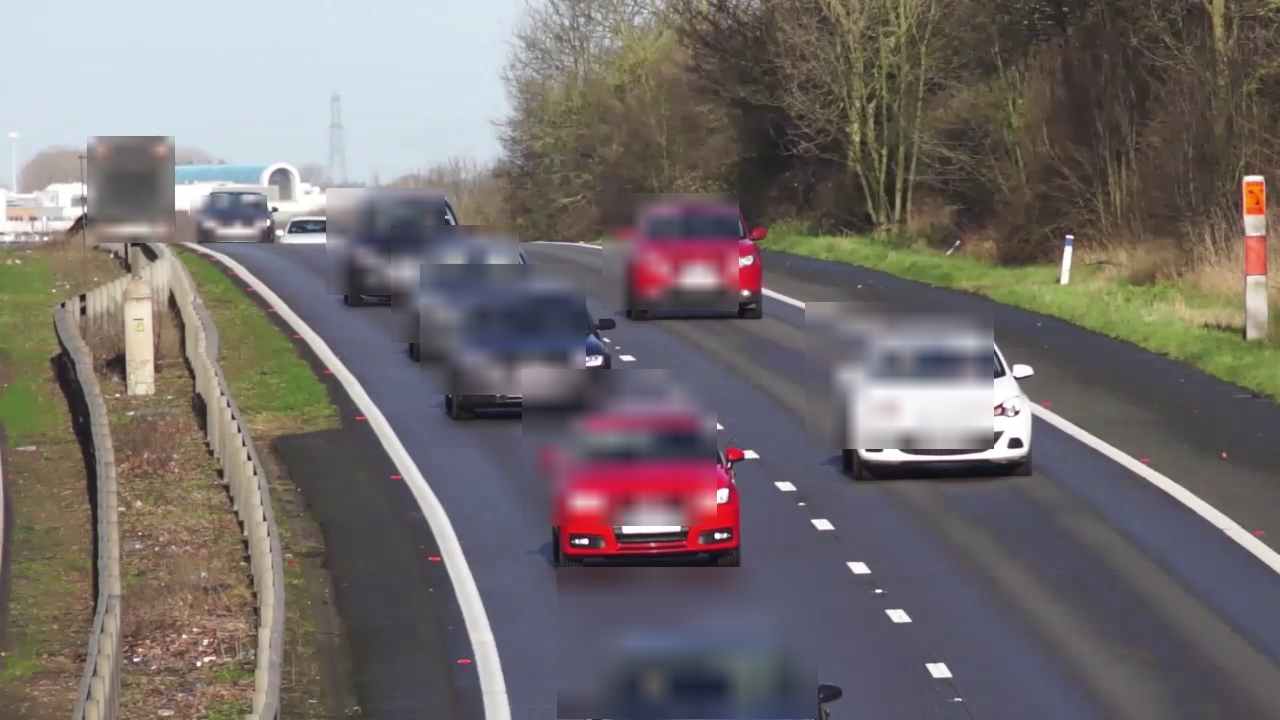
\includegraphics[width=0.85\textwidth]{figures/images/chapter-11/car_kalman_worst_frame.png}
\caption{Worst-frame example from the \texttt{car\_video} sequence using \texttt{detect\_every = 10}. The frame contained nine human-labeled vehicle boxes and ten predicted boxes. The mean \acrshort{iou} was 0.5245, while mean sensitive-region coverage was 0.7469. This illustrates that long prediction intervals can reduce localization accuracy in frames with several nearby moving objects.}
\label{fig:video_prediction_worst_frame_appendix}
\end{figure}

This example shows why both \acrshort{iou} and sensitive-region coverage were used in the main evaluation. The predicted boxes still cover large parts of the sensitive regions, but the alignment is less precise than in easier frames. This makes the frame useful as a qualitative example of the limitations of longer prediction intervals.
% appendices/pen-test.tex

\chapter{Detailed Peneteration Testing and Security Ecaluation}
\label{app:pen_test}

% --------------------------------------------------

\section*{Test 1 --- \texttt{/health} endpoint exposure}

\begin{figure}[h]
    \centering
    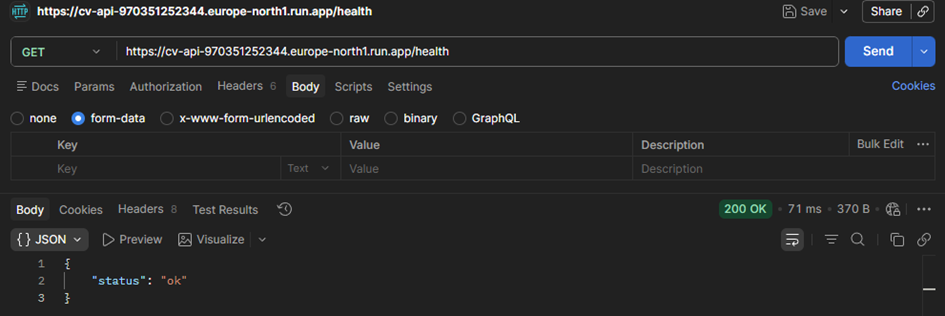
\includegraphics[width=\textwidth]{figures/images/chapter-9/pen-test/health-endpoint-exposure.png}
    \caption{Response from the public \texttt{/health} endpoint}
\end{figure}

\noindent \textbf{Test case:} Public health endpoint inspection

\noindent \textbf{Endpoint:} \texttt{GET /health}

\noindent \textbf{What was sent:} A simple \texttt{GET} request.

\noindent \textbf{Expected result:} A minimal status response without unnecessary internal information.

\noindent \textbf{Actual result:} The endpoint returned \texttt{200 OK} with the minimal JSON response \texttt{\{"status": "ok"\}}. No internal system details, debug data, or sensitive information were exposed.

\noindent \textbf{Assessment:} Worked as expected. The endpoint exposes only minimal health status information and does not appear to leak unnecessary internal data.

% --------------------------------------------------

\section*{Test 1 --- Valid \texttt{/api/detect} request}

\begin{figure}[H]
    \centering
    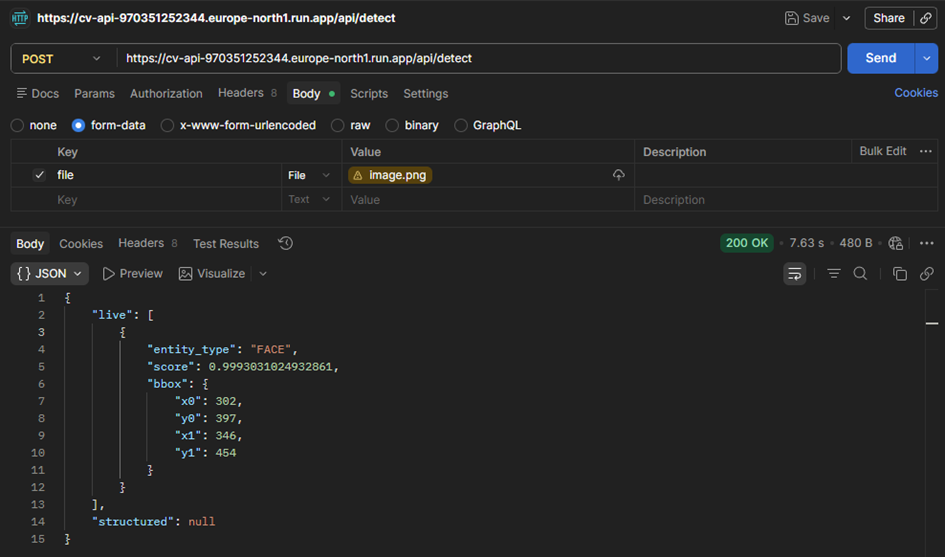
\includegraphics[width=\textwidth]{figures/images/chapter-9/pen-test/valid-api-detect-request.png}
    \caption{Response from a valid request to \texttt{/api/detect}}
\end{figure}

\noindent \textbf{Test case:} Valid image upload to \texttt{/api/detect} 

\noindent \textbf{Endpoint:} \texttt{POST /api/detect} 

\noindent \textbf{What was sent:} A normal image file using multipart form-data. 

\noindent \textbf{Expected result:} The API should return \texttt{200 OK} with detection results. 

\noindent \textbf{Actual result:} The API returned \texttt{200 OK}. The response contained detection output, including \texttt{entity\_type: "FACE"}, a confidence score, and bounding box coordinates. 

\noindent \textbf{Assessment:} Worked as expected. 

% --------------------------------------------------

\section*{Test 2 --- Invalid file disguised as image}

\begin{figure}[H]
    \centering
    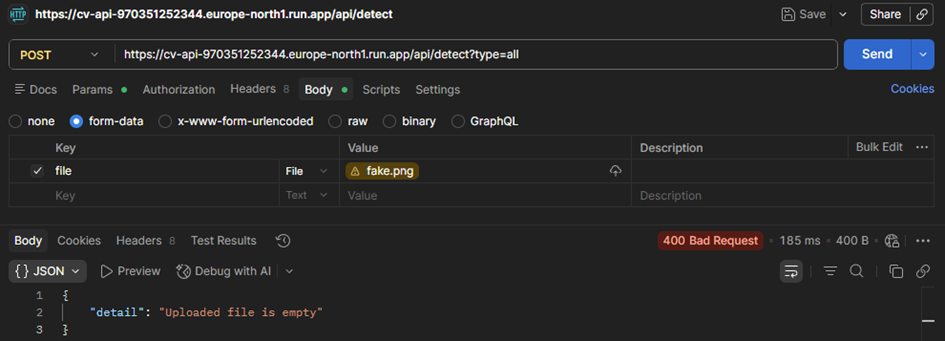
\includegraphics[width=\textwidth]{figures/images/chapter-9/pen-test/fake-image-test.png}
    \caption{Response from invalid file upload to \texttt{/api/detect}}
\end{figure}

\noindent \textbf{Test case:} Invalid file disguised as image 

\noindent \textbf{Endpoint:} \texttt{POST /api/detect} 

\noindent \textbf{What was sent:} An empty text file renamed to \texttt{.jpg} and uploaded as multipart form-data. 

\noindent \textbf{Expected result:} The API should reject the file without crashing and return an appropriate client error response. 

\noindent \textbf{Actual result:} The API returned \texttt{400 Bad Request} with the message \texttt{"Uploaded file is empty"}. 

\noindent \textbf{Assessment:} Worked as expected. The invalid input was handled safely, and the API returned a proper client-side error. 

% --------------------------------------------------

\section*{Test 4 --- Invalid JSON in \texttt{/api/redact}}

\begin{figure}[H]
    \centering
    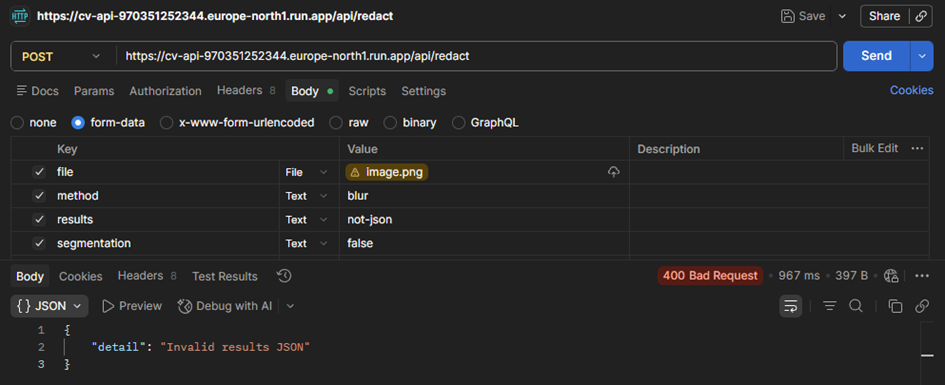
\includegraphics[width=\textwidth]{figures/images/chapter-9/pen-test/redact-invalid-json.png}
    \caption{Response from invalid JSON input to \texttt{/api/redact}}
\end{figure}

\noindent \textbf{Test case:} Invalid JSON in results for \texttt{/api/redact} 

\noindent \textbf{Endpoint:} \texttt{POST /api/redact} 

\noindent \textbf{What was sent:} A valid image, \texttt{method=blur}, \texttt{results=not-json}, and \texttt{segmentation=false}. 

\noindent \textbf{Expected result:} The API should reject the request with a controlled error. 

\noindent \textbf{Actual result:} The API returned \texttt{400 Bad Request} with the message \texttt{"Invalid results JSON"}. 

\noindent \textbf{Assessment:} Worked as expected. The invalid input was handled safely, and the API returned a proper client-side error without crashing. 

% --------------------------------------------------

\section*{Test 6 --- Invalid method in \texttt{/api/redact}}

\begin{figure}[H]
    \centering
    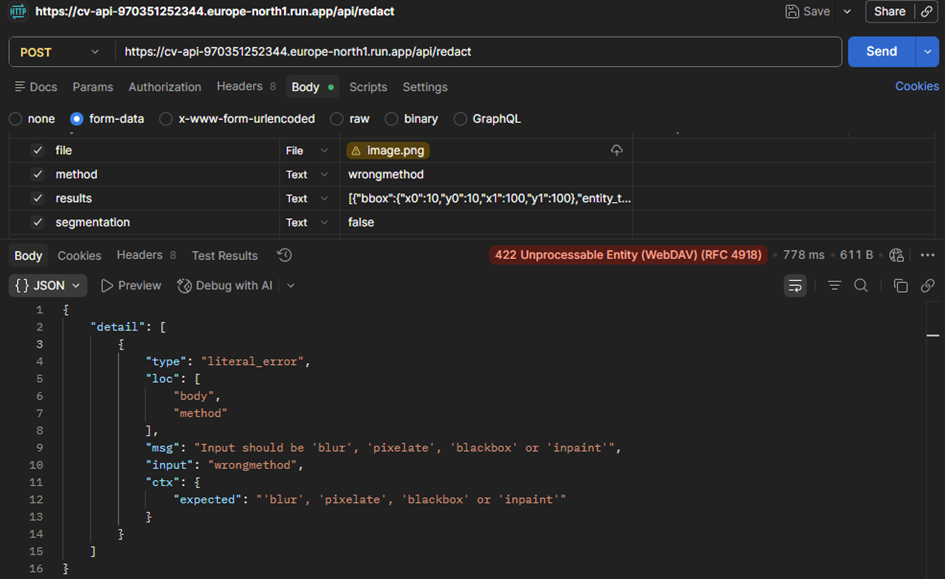
\includegraphics[width=\textwidth]{figures/images/chapter-9/pen-test/invalid-method-redact.png}
    \caption{Response from unsupported method input to \texttt{/api/redact}}
\end{figure}

\noindent \textbf{Test case:} Unsupported redaction method

\noindent \textbf{Endpoint:} \texttt{POST /api/redact}

\noindent \textbf{What was sent:} A valid request with a valid image and results payload, but with \texttt{method=wrongmethod}.

\noindent \textbf{Expected result:} The API should reject the request with a validation error.

\noindent \textbf{Actual result:} The API returned \texttt{422 Unprocessable Entity} with a validation message stating that the input should be \texttt{"blur"}, \texttt{"pixelate"}, \texttt{"blackbox"}, or \texttt{"inpaint"}.

\noindent \textbf{Assessment:} Worked as expected. The invalid method was blocked correctly, and the API returned a controlled validation error without crashing.

% --------------------------------------------------

\section*{Test 7 --- Extreme coordinates in \texttt{/api/redact}}

\begin{figure}[H]
    \centering
    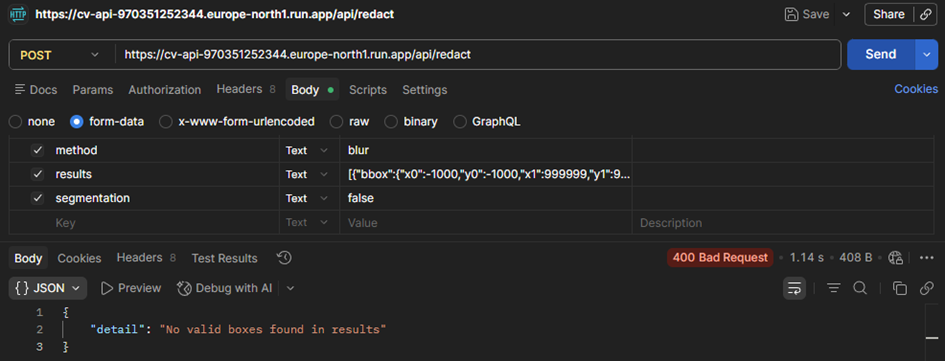
\includegraphics[width=\textwidth]{figures/images/chapter-9/pen-test/extreme-coordinates-redact.png}
    \caption{Response from extreme bounding box coordinates sent to \texttt{/api/redact}}
\end{figure}

\noindent \textbf{Test case:} Extreme bounding box coordinates

\noindent \textbf{Endpoint:} \texttt{POST /api/redact}

\noindent \textbf{What was sent:} A request with very large and negative bounding box coordinates in \texttt{results}: \texttt{[{"bbox":{"x0":-1000,"y0":-1000,"x1":999999,"y1":999999},"entity\_type":"FACE"}]}

\noindent \textbf{Expected result:} The API should handle the request safely without crashing.

\noindent \textbf{Actual result:} The API returned \texttt{400 Bad Request} with the message \texttt{"No valid boxes found in results"}.

\noindent \textbf{Assessment:} Worked as expected. The invalid bounding box coordinates were rejected safely, and the API returned a controlled client-side error without crashing.

% --------------------------------------------------

\section*{Test 10 --- Empty results list on \texttt{/api/redact}}

\begin{figure}[H]
    \centering
    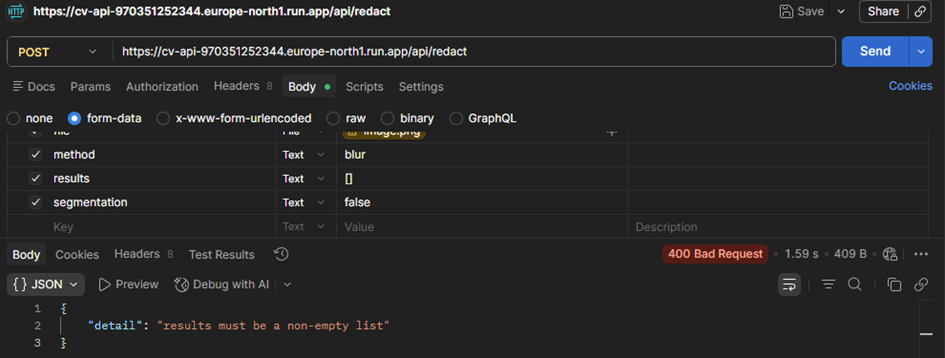
\includegraphics[width=\textwidth]{figures/images/chapter-9/pen-test/empty-results-redact.png}
    \caption{Response from empty \texttt{results} list sent to \texttt{/api/redact}}
\end{figure}

\noindent \textbf{Test case:} Empty results list in \texttt{/api/redact}

\noindent \textbf{Endpoint:} \texttt{POST /api/redact}

\noindent \textbf{What was sent:} A valid image, a valid method, and \texttt{results=[]}.

\noindent \textbf{Expected result:} The API should reject the request with a controlled validation error.

\noindent \textbf{Actual result:} The API returned \texttt{400 Bad Request} with the message \texttt{"results must be a non-empty list"}.

\noindent \textbf{Assessment:} Worked as expected. The empty \texttt{results} list was rejected correctly, and the API returned a controlled client-side error without crashing.

% --------------------------------------------------

\section*{Test 11 --- Malformed results structure on \texttt{/api/redact}}

\begin{figure}[H]
    \centering
    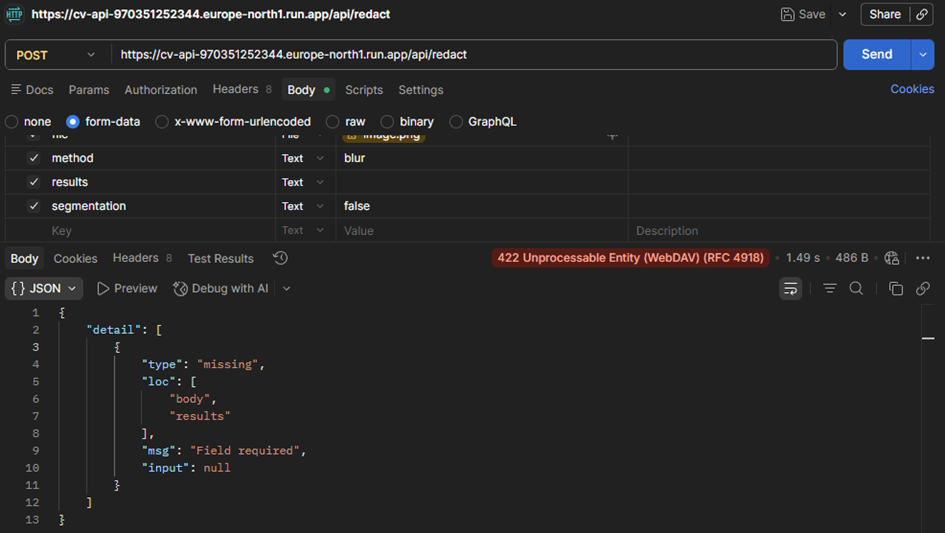
\includegraphics[width=\textwidth]{figures/images/chapter-9/pen-test/malformed-results-redact.png}
    \caption{Response from malformed \texttt{results} input sent to \texttt{/api/redact}}
\end{figure}

\noindent \textbf{Test case:} Malformed results structure in \texttt{/api/redact}

\noindent \textbf{Endpoint:} \texttt{POST /api/redact}

\noindent \textbf{What was sent:} A valid image and valid method, but the \texttt{results} field was malformed and did not contain the required structure. [{"foo":"bar"}]

\noindent \textbf{Expected result:} The API should reject the request or ignore invalid entries safely.

\noindent \textbf{Actual result:} The API returned \texttt{422 Unprocessable Entity} with a validation error stating that the \texttt{results} field was required.

\noindent \textbf{Assessment:} Worked as expected. The malformed input was handled safely, and the API rejected the request with a controlled validation error.

% --------------------------------------------------

\section*{Test 13 --- Many boxes in \texttt{/api/redact}}

\begin{figure}[H]
    \centering
    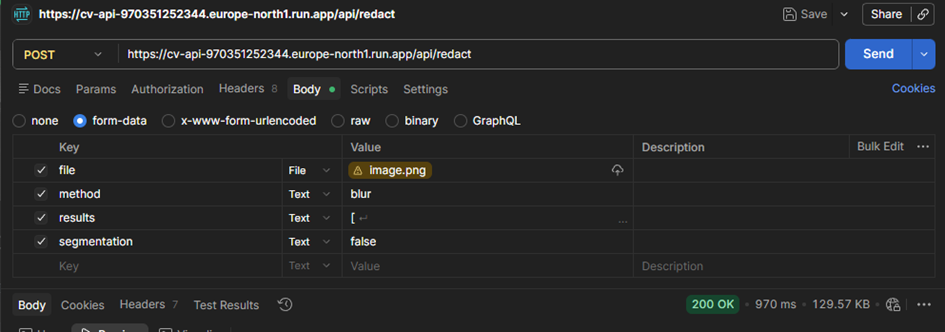
\includegraphics[width=\textwidth]{figures/images/chapter-9/pen-test/many-boxes-redact.png}
    \caption{Response from a \texttt{/api/redact} request with many bounding boxes}
\end{figure}

\noindent \textbf{Test case:} Large number of boxes in \texttt{/api/redact}

\noindent \textbf{Endpoint:} \texttt{POST /api/redact}

\noindent \textbf{What was sent:} A request containing many bounding boxes in the \texttt{results} field. The full payload is not visible in the screenshot because the Postman UI truncates long field values.

\noindent \textbf{Expected result:} The API should remain stable and either complete the request or fail in a controlled way.

\noindent \textbf{Actual result:} The API returned \texttt{200 OK} after approximately \texttt{970 ms}. The request completed successfully and returned a response body of approximately \texttt{129.57 kB}.

\noindent \textbf{Assessment:} Worked as expected. The endpoint remained stable under heavier input and completed the request successfully.

% --------------------------------------------------

\section*{Test 14 --- Invalid query parameters on \texttt{/api/detect}}

\begin{figure}[H]
    \centering
    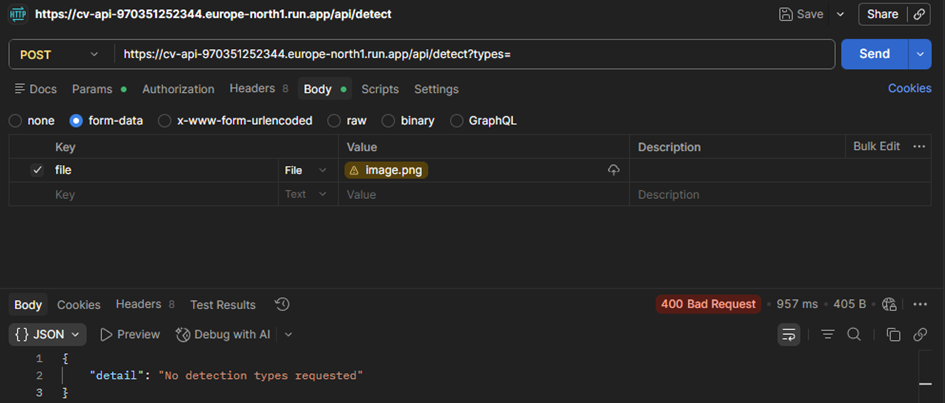
\includegraphics[width=\textwidth]{figures/images/chapter-9/pen-test/invalid-query-parameters-detect.png}
    \caption{Response from invalid query parameters sent to \texttt{/api/detect}}
\end{figure}

\noindent \textbf{Test case:} Invalid query parameters in \texttt{/api/detect}

\noindent \textbf{Endpoint:} \texttt{POST /api/detect}

\noindent \textbf{What was sent:} A request with an empty \texttt{types} query parameter value, shown as \texttt{/api/detect?types=}.

\noindent \textbf{Expected result:} The API should reject invalid parameter combinations safely.

\noindent \textbf{Actual result:} The API returned \texttt{400 Bad Request} with the message \texttt{"No detection types requested"}.

\noindent \textbf{Assessment:} Worked as expected. The invalid query parameter value was handled safely, and the API returned a controlled client-side error without crashing.

% --------------------------------------------------

\section*{Test 23 --- Very large request body / oversized file}

\begin{figure}[h]
    \centering
    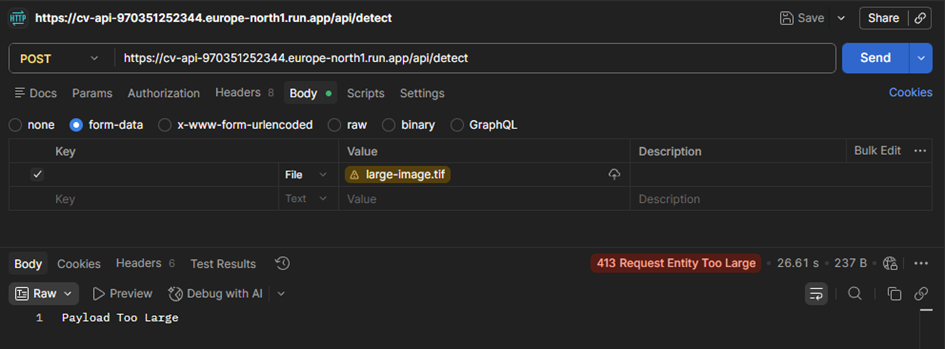
\includegraphics[width=\textwidth]{figures/images/chapter-9/pen-test/oversized-file-detect.png}
    \caption{Response from an oversized file upload sent to \texttt{/api/detect}}
\end{figure}

\noindent \textbf{Test case:} Oversized file upload

\noindent \textbf{Endpoint:} \texttt{POST /api/detect}

\noindent \textbf{What was sent:} A very large image file, shown as \texttt{large-image.tif}.

\noindent \textbf{Expected result:} The API should remain stable and either process the file or fail in a controlled way.

\noindent \textbf{Actual result:} The API returned \texttt{413 Request Entity Too Large} with the message \texttt{Payload Too Large}. The response was returned after approximately \texttt{26.61 s}, so the request was rejected in a controlled way rather than timing out or crashing.

\noindent \textbf{Assessment:} Worked as expected. The oversized upload was handled safely with a controlled error response. However, the response time was relatively high, so upload rejection could potentially be made faster depending on where size validation is enforced.

% --------------------------------------------------



% --------------------------------------------------

\section*{Test 8 --- Browser storage inspection}

\begin{figure}[H]
    \centering
    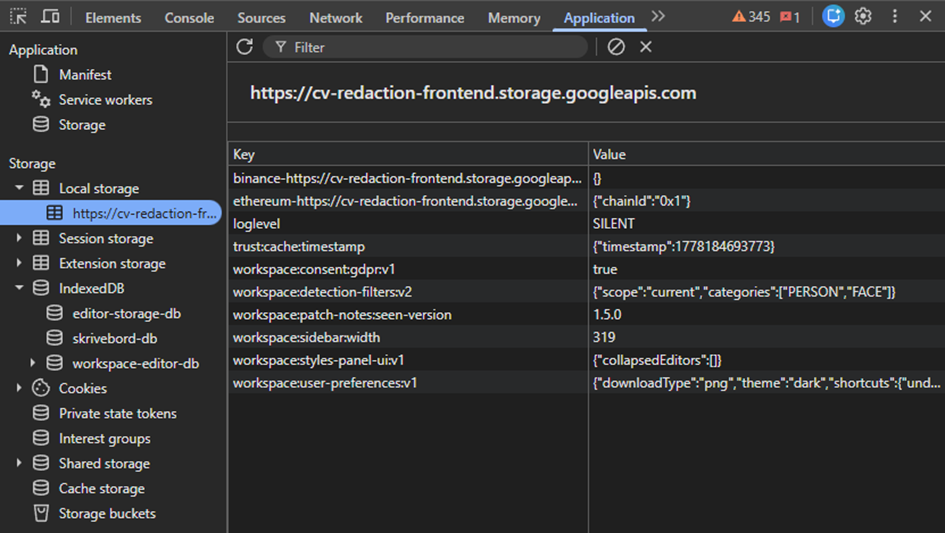
\includegraphics[width=\textwidth]{figures/images/chapter-9/pen-test/browser-storage-inspection.png}
    \caption{Local browser storage entries for the frontend application}
\end{figure}

\noindent \textbf{Test case:} Client-side storage inspection

\noindent \textbf{What was checked:} Browser storage used by the frontend application.

\noindent \textbf{Expected result:} Only local preferences, annotations, or workflow-related state should be stored client-side.

\noindent \textbf{Actual result:} Local storage contained mainly frontend state and preference data, including detection filter settings, consent state, patch notes version, sidebar width, editor UI state, and user preferences such as theme and download type. The view also showed \texttt{binance-...} and \texttt{ethereum-...} entries, which may come from browser wallet integrations or extensions rather than the application itself.

\noindent \textbf{Assessment:} Worked as expected. The stored data appears to be mostly UI preferences and workflow-related client state, which is consistent with a privacy-friendly design. However, this data remains on the client device, and some entries may originate from browser extensions rather than the frontend itself.
% appendices/pen-test.tex

\chapter{Mathematical Model and Verification Script for Redaction Irreversibility}
\label{app:redaction_irreversibility}

This appendix documents the mathematical basis and verification script used for the redaction irreversibility evaluation in Section~\ref{sec:irreversibility-verification}. The purpose is to show why destructive pixel replacement is not reversible from the exported file alone, and to document how the pixel-level verification was performed.

\section{Mathematical Model}

A digital image can be represented as an array or matrix of pixel values. Gonzalez and Woods define an image as a two-dimensional function \(f(x,y)\), where \(x\) and \(y\) are spatial coordinates, and the value of the function represents the image intensity at that point~\cite{gonzalez2018digital}. For colour images, each pixel contains several channel values, such as red, green, and blue in the RGB colour model. The image can therefore be modelled as:

\[
I \in \{0,\ldots,255\}^{H \times W \times C},
\]

where \(H\) is the image height, \(W\) is the image width, and \(C\) is the number of colour channels. For an RGB image, \(C=3\). Let \(R\) denote the region selected for redaction.

A destructive black box redaction function \(F\) produces an exported image \(J\) such that:

\[
J(x,y,c) =
\begin{cases}
k_c, & \text{if } (x,y) \in R, \\
I(x,y,c), & \text{if } (x,y) \notin R,
\end{cases}
\]

where \(k\) is a constant colour value, for example \(k=(0,0,0)\) for black redaction.

This operation removes the original pixel values inside \(R\). The mathematical reason this cannot be reversed uniquely follows from the standard property of inverse functions: a function must be one-to-one in order to have a unique inverse on its image~\cite{rosen2019discrete}. To illustrate this, consider two different original images \(I_1\) and \(I_2\) that are identical outside \(R\), but different inside \(R\). After black box redaction, both images contain the same constant values inside \(R\), and the same unchanged pixels outside \(R\). Therefore,

\[
F(I_1,R) = F(I_2,R)
\]

even though

\[
I_1 \neq I_2.
\]

The function is therefore not injective. Since multiple different original images can produce the same exported redacted image, no unique inverse function exists that can reconstruct the original content from the exported file alone~\cite{rosen2019discrete}. This is consistent with redaction guidance from The National Archives, which states that redaction must irreversibly remove the required information from the redacted copy and remove it from the underlying bitstream rather than only from the visible display~\cite{nationalarchives_redaction_toolkit}. The same principle is also reflected in guidance from the Information Commissioner's Office, which describes the purpose of redaction as irreversibly removing exempt information from the redacted copy~\cite{ico_disclose_safely}.

This irreversibility depends on the original pixels being destructively overwritten and not preserved in hidden layers, metadata, embedded previews, caches, or external copies. For this reason, the verification also included a metadata check. This is aligned with guidance on de-identification and safe disclosure, which treats redaction as a removal-based de-identification technique~\cite{nist800188}. The ICO guidance further illustrates that visually hiding information with a black box is not sufficient if the underlying electronic file still contains the original information~\cite{ico_disclose_safely}.

\begin{lstlisting}[language=Python, caption={Pixel-level verification script for exported redaction}, label={lst:redaction-verification-script}]
from PIL import Image, ExifTags
import numpy as np
import json
import os


# ============================================================
# Configuration
# ============================================================

ORIGINAL_PATH = "cat-original.jpg"
REDACTED_PATH = "cat-redacted.png"

# Coordinates returned by the backend in the original image coordinate space.
REGION_ORIGINAL = {
    "x1": 823,
    "y1": 499,
    "x2": 2562,
    "y2": 2950,
}

# Expected colour for black box redaction.
EXPECTED_COLOR = np.array([0, 0, 0])

# Tolerance used when checking for black or near-black pixels.
# A small tolerance accounts for scaling, anti-aliasing, or export effects.
TOLERANCE = 15

# Acceptance criteria for the verification.
MIN_BLACK_LIKE_PERCENTAGE = 99.0
MIN_CHANGED_PERCENTAGE = 99.0

MAX_SAMPLE_COLORS = 10


# ============================================================
# Helper functions
# ============================================================

def load_rgb_image(path: str) -> Image.Image:
    if not os.path.exists(path):
        raise FileNotFoundError(f"File not found: {path}")

    return Image.open(path).convert("RGB")


def get_metadata(path: str) -> dict:
    image = Image.open(path)

    metadata = {
        "format": image.format,
        "mode": image.mode,
        "size": image.size,
        "info_keys": list(image.info.keys()),
    }

    exif_data = image.getexif()
    exif_readable = {}

    if exif_data:
        for tag_id, value in exif_data.items():
            tag = ExifTags.TAGS.get(tag_id, tag_id)
            exif_readable[str(tag)] = str(value)

    metadata["exif"] = exif_readable
    return metadata


def clamp_region(region: dict, width: int, height: int) -> dict:
    return {
        "x1": max(0, min(int(region["x1"]), width - 1)),
        "y1": max(0, min(int(region["y1"]), height - 1)),
        "x2": max(0, min(int(region["x2"]), width)),
        "y2": max(0, min(int(region["y2"]), height)),
    }


def scale_region(region: dict, scale_x: float, scale_y: float) -> dict:
    return {
        "x1": round(region["x1"] * scale_x),
        "y1": round(region["y1"] * scale_y),
        "x2": round(region["x2"] * scale_x),
        "y2": round(region["y2"] * scale_y),
    }


def validate_region(region: dict) -> None:
    if region["x2"] <= region["x1"]:
        raise ValueError(f"Invalid region: x2 must be greater than x1: {region}")

    if region["y2"] <= region["y1"]:
        raise ValueError(f"Invalid region: y2 must be greater than y1: {region}")


def unique_colors_sample(region_pixels: np.ndarray, max_colors: int = 10) -> tuple[int, list]:
    unique_colors = np.unique(region_pixels.reshape(-1, 3), axis=0)
    return len(unique_colors), unique_colors[:max_colors].tolist()


def percentage(part: int, total: int) -> float:
    if total == 0:
        return 0.0
    return part / total * 100


# ============================================================
# Verification
# ============================================================

def main():
    result = {}

    original_img = load_rgb_image(ORIGINAL_PATH)
    redacted_img = load_rgb_image(REDACTED_PATH)

    original = np.array(original_img)
    redacted = np.array(redacted_img)

    original_h, original_w = original.shape[:2]
    redacted_h, redacted_w = redacted.shape[:2]

    result["files"] = {
        "original": ORIGINAL_PATH,
        "redacted": REDACTED_PATH,
    }

    result["original_size"] = {
        "width": original_w,
        "height": original_h,
    }

    result["redacted_size"] = {
        "width": redacted_w,
        "height": redacted_h,
    }

    same_size = original.shape == redacted.shape
    result["same_size"] = bool(same_size)

    # Compute scaling between the original image and the exported image.
    scale_x = redacted_w / original_w
    scale_y = redacted_h / original_h

    result["scale"] = {
        "scale_x": scale_x,
        "scale_y": scale_y,
        "uniform_scaling_approx": bool(abs(scale_x - scale_y) < 0.01),
    }

    # Resize the original image to the exported image size if necessary.
    # This allows both images to be compared in the same pixel coordinate space.
    if not same_size:
        original_img_resized = original_img.resize(
            (redacted_w, redacted_h),
            Image.Resampling.LANCZOS,
        )
        original_for_comparison = np.array(original_img_resized)
    else:
        original_for_comparison = original

    # Convert backend coordinates to the coordinate space of the exported image.
    region_scaled = scale_region(REGION_ORIGINAL, scale_x, scale_y)
    region_scaled = clamp_region(region_scaled, redacted_w, redacted_h)
    validate_region(region_scaled)

    result["region_original_coordinates"] = REGION_ORIGINAL
    result["region_scaled_to_redacted_image"] = region_scaled

    x1 = region_scaled["x1"]
    y1 = region_scaled["y1"]
    x2 = region_scaled["x2"]
    y2 = region_scaled["y2"]

    region_width = x2 - x1
    region_height = y2 - y1
    region_pixel_count = region_width * region_height

    result["region_dimensions_scaled"] = {
        "width": region_width,
        "height": region_height,
        "pixel_count": int(region_pixel_count),
    }

    original_region = original_for_comparison[y1:y2, x1:x2, :]
    redacted_region = redacted[y1:y2, x1:x2, :]

    if original_region.shape != redacted_region.shape:
        raise ValueError(
            f"Region shape mismatch: original={original_region.shape}, "
            f"redacted={redacted_region.shape}"
        )

    # Check whether the exported redaction region is black or near-black.
    difference_from_expected = np.abs(
        redacted_region.astype(int) - EXPECTED_COLOR.astype(int)
    )

    black_like_pixels = np.all(difference_from_expected <= TOLERANCE, axis=2)

    black_like_pixel_count = int(np.sum(black_like_pixels))
    total_blackbox_pixels = int(black_like_pixels.size)
    black_like_percentage = percentage(
        black_like_pixel_count,
        total_blackbox_pixels,
    )

    is_black_like = black_like_percentage >= MIN_BLACK_LIKE_PERCENTAGE

    max_difference_from_black = int(np.max(difference_from_expected))
    mean_difference_from_black = float(np.mean(difference_from_expected))

    redacted_unique_count, redacted_unique_sample = unique_colors_sample(
        redacted_region,
        MAX_SAMPLE_COLORS,
    )

    result["blackbox_check"] = {
        "expected_color": EXPECTED_COLOR.tolist(),
        "tolerance": TOLERANCE,
        "min_black_like_percentage_required": MIN_BLACK_LIKE_PERCENTAGE,
        "redacted_region_is_black_like": bool(is_black_like),
        "black_like_pixel_count": black_like_pixel_count,
        "total_pixels_checked": total_blackbox_pixels,
        "black_like_percentage": black_like_percentage,
        "max_difference_from_black": max_difference_from_black,
        "mean_difference_from_black": mean_difference_from_black,
        "redacted_region_unique_color_count": int(redacted_unique_count),
        "sample_unique_colors_in_redacted_region": redacted_unique_sample,
    }

    # Compare the exported region with the corresponding original region.
    pixels_equal = np.all(original_region == redacted_region, axis=2)

    equal_pixel_count = int(np.sum(pixels_equal))
    total_pixels = int(pixels_equal.size)
    changed_pixel_count = total_pixels - equal_pixel_count
    changed_percentage = percentage(changed_pixel_count, total_pixels)

    original_unique_count, original_unique_sample = unique_colors_sample(
        original_region,
        MAX_SAMPLE_COLORS,
    )

    result["pixel_comparison_in_region"] = {
        "min_changed_percentage_required": MIN_CHANGED_PERCENTAGE,
        "total_pixels": total_pixels,
        "pixels_equal": equal_pixel_count,
        "pixels_changed": changed_pixel_count,
        "pixels_changed_percentage": changed_percentage,
        "original_region_unique_color_count": int(original_unique_count),
        "sample_unique_colors_in_original_region": original_unique_sample,
    }

    # Check metadata in both files.
    result["metadata"] = {
        "original": get_metadata(ORIGINAL_PATH),
        "redacted": get_metadata(REDACTED_PATH),
    }

    passed = bool(
        black_like_percentage >= MIN_BLACK_LIKE_PERCENTAGE
        and changed_percentage >= MIN_CHANGED_PERCENTAGE
    )

    result["test_passed"] = passed

    if passed:
        result["conclusion"] = (
            "The verification passed. The analysed redaction region in the "
            "exported image was overwritten with black or near-black values, "
            "and the pixel values differ from the corresponding original region."
        )
    else:
        result["conclusion"] = (
            "The verification did not pass. The region, scaling, tolerance, "
            "or exported redaction output should be inspected."
        )

    output_file = "redaction_verification_report.json"

    with open(output_file, "w", encoding="utf-8") as file:
        json.dump(result, file, indent=4, ensure_ascii=False)

    print(json.dumps(result, indent=4, ensure_ascii=False))
    print(f"Report written to: {output_file}")


if __name__ == "__main__":
    main()
\end{lstlisting}
\chapter{Metadata Preservation, Editing, and Provenance Handling}
\label{app:metadata-handling}

\textit{Supplementary research notes for deferred SafeVision metadata functionality.}

\section*{Abstract}
This appendix examines how metadata handling could be added to SafeVision as a future system feature and therefore will be written as a research paper for Safe Media AI. The main SafeVision implementation focused on visible sensitive content in images and videos, such as faces, text, license plates, barcodes, people, and vehicles. Metadata handling was excluded from the final implementation as a scope decision, not because it is technically impossible. The appendix describes why metadata matters, how it could be integrated into the redaction and export pipeline, which technical tools are relevant, and what risks should be considered. It also discusses stakeholder interest in whether metadata can help distinguish AI-generated media from camera-captured or manually edited media.

\section{Motivation}
SafeVision was developed to support detection and redaction of sensitive information in visual media. The implemented system therefore focused on visible content, such as faces, text, license plates, barcodes, people, and vehicles. Metadata handling was not implemented as part of the final system. This was a scope decision rather than a technical impossibility.

A key consideration is that metadata can represent both a privacy risk and a source of operational, legal, or archival value. In some workflows, timestamps, creator fields, copyright information, camera data, or color profiles may have documentation value. In other workflows, the same fields may reveal sensitive information and should be removed or modified before sharing. A complete metadata feature should therefore be designed around explicit user control rather than automatic removal only.

Another motivation came from stakeholder interest in whether metadata could help distinguish AI-generated images or videos from camera-captured or manually edited media. This question is increasingly relevant because synthetic visual content is becoming more realistic and harder to assess through visual inspection alone. Metadata can support this task when a file contains provenance information, such as C2PA Content Credentials. However, ordinary EXIF, IPTC, or XMP fields should not be treated as a reliable AI-detection method, because they can be edited, removed, or regenerated during normal processing.

Export behavior is also relevant. When an image or video is redacted, the application often creates a new output file rather than modifying the original file in place. Depending on the export method, original metadata may be stripped, regenerated, or partially preserved. Browser canvas export, for example, creates a new image representation and specifies 96 dpi resolution metadata for formats that support it [6]. Metadata should therefore not be assumed as safely removed or reliably preserved. The safer design is to treat metadata handling as a deliberate export policy.

\section{Relevant Metadata Categories}
A metadata feature would need to handle several categories of information. The most relevant categories are summarized below.

\begin{itemize}[leftmargin=1.5em]
    \item \textbf{EXIF metadata:} Commonly stores camera and capture information, including camera model, lens settings, exposure values, timestamps, GPS coordinates, orientation, and device identifiers. EXIF is especially relevant for privacy because GPS and camera serial fields can identify location or equipment.
    \item \textbf{IPTC metadata:} Often used in journalism, publishing, and archival workflows. It may include captions, keywords, creator information, copyright notices, contact fields, and editorial metadata. This can be valuable for documentation but may also reveal internal or personal information.
    \item \textbf{XMP metadata:} An extensible XML-based metadata format used by many editing and asset-management tools. XMP can mirror or extend EXIF and IPTC fields and is often used to store editing, rights, workflow, and provenance information.
    \item \textbf{ICC profiles:} Color profiles that describe how colors should be interpreted. Unlike many metadata fields, ICC profiles are usually not privacy-sensitive. Removing them may change the visual appearance of the exported image, so preserving ICC profiles can be important for visual consistency.
    \item \textbf{Video container metadata:} Video files may contain metadata at the container, stream, chapter, and program level. This can include creation time, encoder information, device information, GPS fields, title, author, and software tags. The exact metadata support depends on the format, such as MP4, MOV, or MKV.
\end{itemize}

\section{Proposed System Design}
The implementation could add a metadata policy layer at export time. This layer would run after visual redaction has been completed and before the final media file is made available to the user. The layer would decide which metadata fields are copied, edited, removed, or reported.

A metadata-aware export pipeline would consist of five steps:

\begin{enumerate}[leftmargin=1.5em]
    \item Read the original media and extract metadata into a structured internal representation.
    \item Run the existing detection, review, and redaction workflow on the visible media content.
    \item Generate the redacted output image or video.
    \item Apply a selected metadata policy to the exported output.
    \item Validate the final file by reading back the metadata and confirming that the policy was applied.
\end{enumerate}

The policy should be selected by the user or by an organization-level default. The default policy should prioritize privacy while keeping technical quality stable. A reasonable default would remove GPS, device-identifying, author, and workflow fields, while preserving ICC color profiles where possible. This preserves visual consistency without unnecessarily retaining privacy-sensitive information.

\section{Metadata Export Policies}
\begin{table}[htbp]
\centering
\caption{Metadata export policy options for SafeVision.}
\label{tab:metadata-export-policies}
\small
\begin{tabularx}{\textwidth}{|>{\raggedright\arraybackslash}p{0.22\textwidth}|>{\raggedright\arraybackslash}X|>{\raggedright\arraybackslash}p{0.22\textwidth}|>{\raggedright\arraybackslash}p{0.22\textwidth}|}
\hline
\rowcolor{black!75}\color{white}\textbf{Policy} & \color{white}\textbf{Description} & \color{white}\textbf{Best suited for} & \color{white}\textbf{Risk / trade-off} \\
\hline
Privacy-first export & Remove descriptive and identifying metadata, remove GPS, preserve ICC if possible. & External sharing and public release. & May remove useful documentation fields. \\
\hline
Preserve documentation & Preserve selected EXIF/IPTC/XMP fields while removing GPS and direct identifiers. & Internal archives and controlled sharing. & Requires careful field selection and validation. \\
\hline
Remove all metadata & Export with no copied metadata except what the encoder automatically creates. & High-risk sharing where provenance is not needed. & May remove color profiles, rights data, or audit information. \\
\hline
Edit before export & Allow users to modify fields such as creator, copyright, caption, keywords, and date. & Professional or archive workflows. & Requires UI support and metadata validation. \\
\hline
Sidecar export & Store metadata in a separate XMP or JSON report rather than embedding it in the redacted media. & Audit trails and documentation without public embedding. & Sidecar files must be managed securely. \\
\hline
\end{tabularx}
\end{table}

A metadata sidecar is useful when the system should keep a record of what was removed or changed without embedding this information in the shared media file. ExifTool supports copying metadata from one file to another and generating sidecar-style metadata outputs, including XMP workflows [4].

\section{Image Metadata Implementation}
For images, metadata handling can be implemented in the backend. Python libraries provide practical support for reading, writing, and modifying different metadata types. Pillow supports image saving options such as EXIF and ICC profile preservation for several formats [1]. Piexif can load, dump, insert, remove, and transplant EXIF data for JPEG, WebP, and TIFF files [2]. IPTCInfo3 can read and modify IPTC metadata in JPEG images [3]. For broader metadata support, ExifTool is often the most robust option because it supports EXIF, IPTC, XMP, ICC profiles, and many file formats [4, 5].

A typical image workflow would read metadata before redaction, apply redaction to pixel data, and then write only the selected metadata back to the exported image. GPS fields could be removed, ICC profiles could be preserved, and selected IPTC or XMP fields could be retained or edited.

Validation is important. Metadata standards overlap, and the same logical field may appear in multiple places. For example, a creator field may exist in IPTC and XMP. A correct implementation should check the exported file after writing, rather than assuming that the requested policy was applied successfully.

\section{Video Metadata Implementation}
Video metadata handling is possible but more complex than image metadata handling. Video files have container-level metadata and may also contain stream-level metadata. FFmpeg provides options for setting metadata values and for controlling metadata mapping between input and output files [7, 8]. ExifTool can also inspect and edit metadata in many video formats [4].

Video metadata handling should be implemented as part of the export stage after video redaction or transcoding. A privacy-focused export could remove input metadata, while a documentation-focused export could preserve or rewrite selected fields such as title, copyright, or case reference.

The exact implementation would depend on the final video pipeline. If Safe Media AI chooses to transcode video during redaction, then metadata can be rewritten during that same export step. If the system attempts stream copying, fewer processing steps may be needed, but metadata behavior must still be verified. FFmpeg concepts such as \texttt{-map\_metadata -1} for preventing inherited metadata and \texttt{-metadata key=value} for setting selected fields illustrate how these policies can be expressed in a video export pipeline [7, 8].

\section{Metadata and AI-Generated Media Provenance}
Interest from the SkannKontroll user test raised an additional use, whether metadata can help distinguish AI-generated images and videos from camera-captured or manually edited media. This is a relevant motivation for future metadata work, but it must be framed carefully. Ordinary metadata can provide clues, but it cannot reliably prove whether media is AI-generated.

The strongest metadata-based approach is not ordinary EXIF or IPTC inspection, but verifiable provenance. The Coalition for Content Provenance and Authenticity (C2PA) provides an open technical standard for establishing the origin and edit history of digital content [9]. Content Credentials are based on this standard and can describe how a file was created or edited [10]. The C2PA technical specification also describes how C2PA manifests can be embedded in assets, including AI/ML-related assets [11].

Watermarking is another approach. Google DeepMind describes SynthID as an invisible watermark for AI-generated images and video segments that are added when content is created and designed to survive common modifications such as cropping, filtering, frame-rate changes, and lossy compression [12]. Google support documentation states that if a SynthID watermark is detected, all or part of the media was created or edited by Google AI models. It also states that if a SynthID watermark is not detected, the media may still have been created by other AI systems [13].

These findings suggest that metadata handling is most useful as provenance support, not as a definitive AI-generation detector. A system should not claim to detect AI-generated media based only on ordinary metadata. Instead, it could check for C2PA or Content Credentials metadata, preserve provenance data during export, warn users when provenance metadata is missing, and avoid accidentally stripping useful authenticity information during redaction. This would support stakeholders who need to evaluate whether media may be AI-generated, while avoiding misleading certainty.

\section{Suggested User Interface}
A metadata feature should be understandable to non-technical users. The interface should not only provide technical field names but also explain the effect of each policy. A practical design could include a metadata panel during export.

\begin{itemize}[leftmargin=1.5em]
    \item \textbf{Export policy selector:} Options such as removing all metadata, preserving ICC only, preserving selected fields, editing selected fields, or generating report.
    \item \textbf{Sensitive field warnings:} GPS coordinates, camera serial numbers, author fields, internal software tags, and project identifiers should be highlighted.
    \item \textbf{Provenance section:} If C2PA or similar provenance data is detected, the interface should show that provenance exists and ask whether it should be preserved.
    \item \textbf{Preview before export:} The user should see which metadata fields will be kept, removed, modified, or unsupported.
    \item \textbf{Export report:} A small report could document the policy used and the result of metadata validation after export.
\end{itemize}

\section{Risks and Limitations}
Metadata handling introduces several technical and workflow-related risks. First, metadata standards overlap. The same information may appear in EXIF, IPTC, and XMP fields, sometimes with inconsistent values. ExifTool notes that EXIF and IPTC standards include mandatory tags and that some tags may be created or removed automatically when writing metadata [5]. This means that metadata changes should always be validated after export.

Second, metadata policies can be misunderstood by users. A user may choose to preserve metadata for documentation purposes without realizing that this also preserves fields such as GPS coordinates, camera serial numbers, or internal software tags. To reduce this risk, the system should not only offer general options such as preserve metadata or remove metadata, but also show which fields will be kept, removed, or modified before export.

Third, metadata support differs between formats. JPEG, PNG, WebP, TIFF, MP4, MOV, and MKV do not handle metadata identically. A metadata policy must therefore be format-aware and should avoid promising that every field can be preserved across every export format. If a field cannot be embedded reliably, the system should offer a sidecar report instead.

Fourth, provenance metadata and watermarking are not universal. C2PA Content Credentials are only useful when the media contains valid credentials and when the workflow preserves them. SynthID can support verification for content generated or edited by Google AI systems, but the absence of a SynthID watermark does not rule out AI generation by other systems [13]. Provenance inspection should therefore be presented as supporting evidence, not as a definitive AI-generation detector.

\section{Conclusion}
Metadata handling was outside the final SafeVision implementation, but it remains a valuable future feature for Safe Media AI. The main requirement is not simply to remove metadata, but to give users explicit control over whether metadata should be removed, preserved, modified, or reported. This is important because metadata can contain sensitive information, but it can also carry documentation, archival, color-management, and provenance value.

Future implementation should add metadata handling as a separate export-policy step. For images, this could be implemented using Pillow, Piexif, IPTCInfo3, and ExifTool depending on the required metadata types. For video, FFmpeg and ExifTool are suitable tools for inspecting and writing container metadata. The implementation should validate metadata after export and provide users with clear explanations of what has changed.

The real user questions about AI-generated media strengthens the motivation for this feature. Metadata cannot reliably determine AI generation on its own, but provenance standards such as C2PA Content Credentials and watermarking systems such as SynthID can provide useful signals when present.


\section*{References}
\begin{enumerate}
    \item[{[1]}] Pillow documentation, ``Image file formats,'' describing image save options and format-specific metadata support. \url{https://pillow.readthedocs.io/en/stable/handbook/image-file-formats.html}
    \item[{[2]}] Piexif documentation, ``Functions,'' describing EXIF load, dump, insert, remove, and transplant operations. \url{https://piexif.readthedocs.io/en/latest/functions.html}
    \item[{[3]}] IPTCInfo3 documentation, ``IPTC Metadata for Python 3,'' describing reading and modifying IPTC metadata in JPEG images. \url{https://james-see.github.io/iptcinfo3}
    \item[{[4]}] Phil Harvey, ExifTool application documentation, describing reading, writing, deleting, copying, and exporting metadata. \url{https://exiftool.org/exiftool_pod.html}
    \item[{[5]}] ExifTool documentation, ``Writing Meta Information,'' describing metadata writing behavior and mandatory EXIF/IPTC tags. \url{https://exiftool.org/writing.html}
    \item[{[6]}] MDN Web Docs, ``HTMLCanvasElement: toBlob() method,'' describing canvas export behavior and 96 dpi metadata. \url{https://developer.mozilla.org/en-US/docs/Web/API/HTMLCanvasElement/toBlob}
    \item[{[7]}] FFmpeg documentation, ``ffmpeg,'' describing stream selection and mapping behavior. \url{https://ffmpeg.org/ffmpeg.html}
    \item[{[8]}] FFmpeg documentation, ``ffmpeg-all,'' describing metadata setting and deletion using the metadata option. \url{https://ffmpeg.org/ffmpeg-all.html}
    \item[{[9]}] Coalition for Content Provenance and Authenticity, ``C2PA: Verifying Media Content Sources,'' describing the C2PA standard for origin and edit history of digital content. \url{https://c2pa.org/}
    \item[{[10]}] Content Credentials, ``Verify Media Authenticity,'' describing Content Credentials and their relationship to C2PA. \url{https://contentcredentials.org/}
    \item[{[11]}] C2PA Technical Specification, describing C2PA manifests and asset assertions. \url{https://spec.c2pa.org/specifications/specifications/2.4/specs/C2PA_Specification.html}
    \item[{[12]}] Google DeepMind, ``SynthID,'' describing invisible watermarking for AI-generated images and video. \url{https://deepmind.google/models/synthid/}
    \item[{[13]}] Google Support, ``Verify Google AI-generated images, videos, and audio with SynthID,'' describing what SynthID detection and non-detection mean. \url{https://support.google.com/gemini/answer/16722517}
\end{enumerate}

% Project plan converted from PDF, prepared as a thesis appendix fragment.
% Include from the main report with: \input{appendices/project-plan_converted}
% Do not compile this file directly: it has no \documentclass, \begin{document}, or \end{document}.
% Expected preamble packages in the main report: graphicx, booktabs, longtable, array, float.
% Optional: enumitem. If enumitem is loaded, list margins are set to match the original project plan style.

\cleardoublepage
\chapter{Project Plan}
\label{app:project-plan}

\begingroup
\setlength{\parindent}{0pt}
\setlength{\parskip}{0.8em}
\makeatletter
\@ifpackageloaded{enumitem}{%
    \setlist[itemize]{leftmargin=*}%
    \setlist[enumerate]{leftmargin=*}%
}{}%
\makeatother
\sloppy

\begin{center}
    {\Large\textbf{Redaction of Sensitive Information in Images}}\\[0.3em]
    {\large Project Plan}\\[0.7em]
    An Hoang Chu, Henrik Weflen Gjermundsen, Karwan Shekhe\\[0.3em]
    Spring 2026
\end{center}

\section{Frame and Goals}

\subsection{Background}

Photographs and videos are commonly used to document places and events in areas such as surveillance, mapping, crime documentation, and journalism. These media may contain sensitive information, defined as data that, if disclosed, can compromise the privacy or safety of individuals or expose confidential information belonging to organizations, including faces, license plates, text, and metadata. When such information is made publicly available, it can lead to risks such as unauthorized identification, tracking, or misuse of personal data. Consequently, handling visual media requires careful consideration of privacy, data protection regulations, and ethical responsibilities.

To safeguard privacy, sensitive information often needs to be removed or obscured. This process is commonly referred to as redaction or censoring. Today, this is frequently performed manually using tools such as Photoshop. Manual editing is time-consuming and may lead to errors when large volumes of data are processed. This creates a need for more efficient and automated solutions.

Advances in artificial intelligence and machine learning have enabled the automated identification and redaction of sensitive content. As a result, several commercial and research-based solutions are available today. However, their quality, functionality, and usability vary significantly. Safe Media AI AS has developed an AI-based platform for editing text-based documents and aims to extend this platform to also support images and potentially video content. As a small startup company, Safe Media AI AS focuses on leveraging artificial intelligence to automatically identify and redact sensitive information.

\subsection{Project Goals}
\label{appsec:goals}

\paragraph{Result Goals}
The goal is to develop and evaluate a solution for automatic and interactive editing of sensitive content in images and potentially video. The solution shall be compatible with existing systems at Safe Media AI AS, support multiple file formats, and comply with requirements related to security and privacy.

Performance and quality will be evaluated both quantitatively and qualitatively. Quantitative evaluation will include metrics such as precision, recall, and F1-score. This captures both missed detections (false negatives) and incorrect redactions (false positives). Qualitative evaluation will assess usability, user experience, and overall effectiveness of the interactive editing features. The solution will also be compared with existing state-of-the-art approaches to highlight improvements in accuracy, efficiency, and user satisfaction.

\paragraph{Impact Goals}
The project aims to improve the efficiency of censoring sensitive information in images and videos through the use of artificial intelligence. The solution is intended to reduce the need for manual work, thereby saving time and resources for users who currently have to manually edit large volumes of visual material.

Another key impact goal is to reduce the risk of human error during the censoring process, ensuring that sensitive information is more accurately identified and anonymized prior to publication or sharing. This will contribute to improved protection of privacy and increased data security.

The project will also enable Safe Media AI AS to offer an extended solution that covers text, images, and video within a single platform. This provides increased value for existing customers and facilitates further commercial use.

\paragraph{Learning Goals}
The project aims to provide the group with increased academic and practical competence in the development of software solutions based on artificial intelligence. Through this work, the group seeks to gain a deeper understanding of how modern AI solutions function in practice and how such technologies can be used to improve efficiency and automate manual work in real-world problem domains.

A key learning objective is to understand how artificial intelligence can be applied as a practical tool in software development, ranging from the integration of existing AI models to the evaluation of performance, quality, and reliability of the solution. This includes gaining insight into how AI-based systems interact with other system components such as backend services and user interfaces.

The project also aims to strengthen skills related to collaboration and working methodologies in larger development projects. Through long-term teamwork, the group seeks to gain experience in clear communication, task allocation, and coordination, which are essential for project progress and quality. Furthermore, an important learning goal is to apply the Scrum methodology in practice through sprint-based work, including task planning and prioritization. In addition, the project will provide experience in collaborating with a product owner to gain a better understanding of agile development processes as used in professional software development projects.

\subsection{Frameworks}

The frameworks guiding this project are as follows:

\paragraph{Technological Frameworks}
The project builds upon existing solutions developed by Safe Media AI AS, and further development will be based on their artificial intelligence technology. Backend development will primarily be carried out using Python and its associated libraries. The specific libraries to be used have not yet been finalized and will be selected during development based on project requirements.

Frontend development will primarily utilize the React framework in combination with Vite as a build tool, enabling efficient development, fast build times, and a modern development workflow. This approach is chosen to ensure seamless integration with Safe Media AI AS' existing solutions while maintaining flexibility and scalability. If project requirements change or the solution becomes diddicukt to solve with these tools, alternative frameworks or technologies may be considered.

The solution will initially focus on processing still images, with the goal of identifying and anonymizing sensitive information such as faces and text.

\paragraph{Deployment and Infrastructure}
Google Cloud will be used as the project's Infrastructure as a Service (IaaS) platform, providing hosting for servers, databases, and additional storage services. The project will be deployed with Docker and support PDF, PNG and JPEG.

\paragraph{Methodological Frameworks}
The project will follow the Scrum methodology as the framework for development. This includes working in short sprints, conducting daily stand-up meetings (daily scrum), sprint planning, sprint reviews, and sprint retrospectives. The workflow will be organized using a Kanban board to provide an overview of tasks, priorities, and progress. Version control will be managed using Git, while project management will be handled through Jira. Code changes will be quality assured through the use of issues and merge requests.

\paragraph{Testing Frameworks}
Unit testing will be applied to both backend and frontend components throughout development to ensure correct functionality. In addition, user testing will be conducted to verify overall system coherence and usability. Postman will be used for API testing to ensure reliable data exchange between system components.

\paragraph{Storage Constraints}
Images and modified images will not be stored at all. They will only exist on the website through IndexedDB to have some data persistence on the website. The server will only receive, detect and the redact and not store anything.

\paragraph{Time Constraints}
The project will be carried out within the specified timeframe during the spring of 2026, with final submission of the bachelor's thesis scheduled for May 20, 2026. The scope of the work is limited to the development and evaluation of a functional prototype, and long-term operation or maintenance is not included.

\paragraph{General Data Protection Regulation Compliance and Security}
GDPR compliance is an important consideration in this project, as the solution processes images that may contain personal data such as faces and license plates. The system is designed in line with the principles of privacy by design and data minimization, ensuring that only necessary data is processed.

Images are not stored on the server at any point and are only processed temporarily for redaction. Limited client-side persistence is handled through IndexedDB to support usability without transmitting or retaining data beyond the user's environment. All communication between system components is secured, and sensitive information is anonymized through redaction prior to use or sharing.

\section{Scope}

\subsection{Subject Area}

The project belongs to the field of data engineering (BIDATA), with a primary focus on artificial intelligence, image processing, as well as security within these domains. The work combines methods from machine learning and computer vision with system development, aiming to create software capable of analyzing and processing visual content in an efficient and reliable manner.

The subject area includes the development and integration of AI-based solutions into complete software systems, encompassing backend services and infrastructure. The project also addresses key challenges related to secure data processing, where requirements for confidentiality, integrity, and correct handling of sensitive information are central.

Throughout the project, theoretical knowledge acquired during the study program is applied in a practical context, with an emphasis on how AI technologies can be used to solve real-world challenges related to privacy and security when publishing and sharing visual material.

\subsection{Task Description}

The task is to design, develop, and evalute an AI-based software sokution for the automatic removal or anonymazation of sensitive information in still images. If time permits, the solution may be extended to support videos as well. The system shall be capable of identifying elements such as faces and text and edit them in a manner that preserves privacy. This works by sending in images and the AI will give a preview on whatever you wanted to be redacted. The editing process itself will happen with one picture at a time or in bulks depending on what the user needs. The solution is required to be user-friendly, support multiple file formats, and offer both automatic and user-controlled editing. Furthermore, the solution will be compared with relevant research and existing commercial solutions and evaluated using both quantitative and qualitative methods.

\subsection{Delimitation}

The project is limited to the development and evaluation of a functional software solution within the given timeframe. The solution shall be usable and suitable for further development by Safe Media AI AS; however, long-term maintenance is not included in the scope of the project.

The core scopeof the project is anonymization of sensitive information in still images, including faces, license plates, and buildings. Video support is considered an optional extension and will only be implemented if a robust and stable solution for still images is achived early in the project. If video is included, the scope will be limited to visual redaction only, and audio content (e.g. speech) will not be processed.

The project will include PDF, PNG and JPEG formats, support for other formats will be considered if everything else is working fine.

Most importantly, the project will at all times prioritize security for both users and employees of the commissioning organization. Therefore, particular emphasis is placed on adhering to privacy principles throughout the entire development process.

\section{Project Organization}

\subsection{Responsibilities and Roles}
\label{appsec:group}

\textbf{Backend Developer and Scrum Master (Henrik):}

The Scrum Master is responsible for ensuring that meetings are scheduled and conducted as planned. This role includes keeping track of discussions during meetings and documenting minutes for each meeting. The Scrum Master also ensures effective communication within the team, takes action if issues arise, and facilitates discussions and meetings to maintain progress. Additionaly, he serves as the primary contact point between the team, the Product owner and the supervisor and writes notes under each meeting.

\textbf{Backend Developer and Product manager (Karwan):}

The Product Manager ensures that coding standards and best practices are followed throughout the project. This role defines the overall framework for the product and ensures that all developers are aligned during the development process. In the event of major disagreements regarding functional or non-functional requirements, the Project Manager is responsible for facilitating dialogue between the parties and leading the process toward a resolution.

\textbf{Frontend Developer and Documentation Manager (Hoang):}

As the Documentation Manager, he is responsible for planning, coordinating, and delivering all project documentation within agreed deadlines. He ensures compliance with formal and academic requirements and with guidelines provided by the institution, Product Owner, and supervisor. He performs proofreading and quality assurance prior to submission, maintains consistency in language, terminology, and structure, and ensures that all updates are reflected in the final documentation.

\begin{figure}[H]
    \centering
    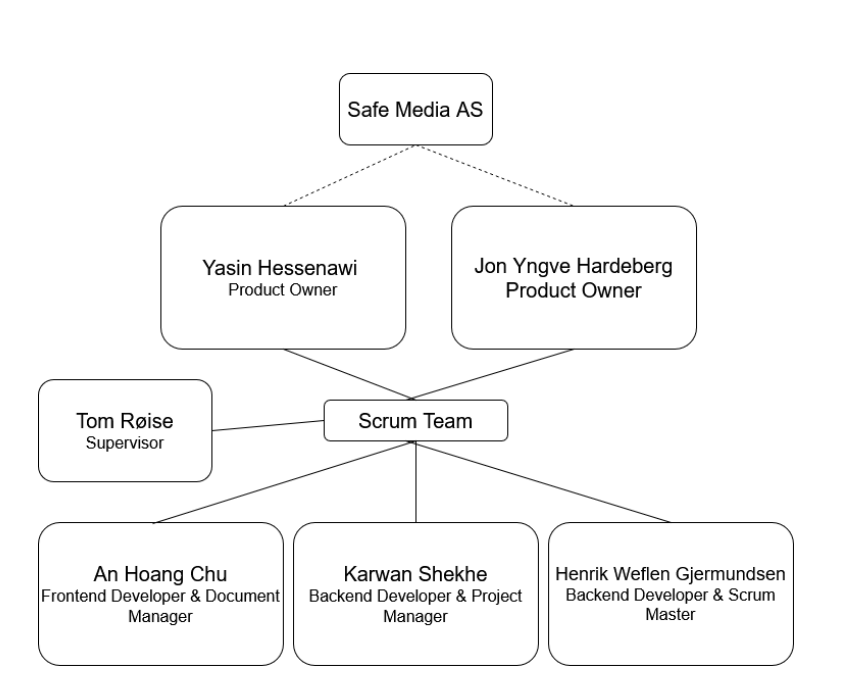
\includegraphics[width=0.85\textwidth]{appendices/scrum_team.png}
    \caption{Scrum team}
\end{figure}

\subsection{Routines and Group Rules}

The complete set of group rules is included in Appendix A. Some key points are outlined below:

\begin{itemize}
    \item Working hours shall be logged, and each member may additionally describe the tasks completed during the week if desired.
    \item These logs are reviewed during project meetings to provide and receive feedback, allowing the group to discuss the work performed by each member.
    \item The group conducts daily Scrum meetings from Monday to Wednesday.
    \item The group holds a meeting with the supervisor every Monday and meets with the project provider every Thursday.
    \item Meeting minutes shall be written after all meetings.
    \item Each group member is expected to allocate several hours after meetings to work together physically at the same location.
    \item Group members shall use the kanban board to assign and prioritize tasks.
    \item Online communication shall take place via Discord.
\end{itemize}

\section{Planning, Follow-up and Reporting}

\subsection{Main breakdown of the project}
\label{appsec:pfar}

We have chosen to use the agile methodology Scrum together with a Kanban board, also called Scrumban. The reason we chose this model is that, in a project like ours, a number of technical uncertainties can arise along the way, which this type of model is well suited for. Another reason is that almost every organization practices agile methods, and the agile Kanban has seen increased popularity especially in software development. Scrum and Kanban are considered as the two powerful Agile methods that handle and manage the progress of software development (Alaidaros \& Omar, 2017; Lei et al., 2017). With a Kanban board we can set up and get an overview of new tasks that appear during the process, and we get a good visualization of workflow and priorities. At the same time, Scrumban allows us to organize the work into short sprints where we can divide the work into phases based on where we are in the project. This methodology also gives us a way of working where it is easy to get feedback from each other/the supervisor/product owner, implement changes continuously, and maintain a good overview.

The way we follow Scrumban in practice is by using Jira as our management tool. In Jira we create issues that we can organize through the columns ``to do'', ``in progress'', ``to test'', ``in review'', ``done''. This is done so that we can visualize the workflow and identify bottlenecks, so tasks do not pile up. This sprint backlog can be updated in connection with the daily scrum, so that we remain flexible during the sprint. Code changes are done via merge requests in GitHub and quality-assured by the rest of the group before it goes into the main branch (see 5.1). An issue is considered finished when it has been confirmed as implemented by everyone in the group and documented to the necessary degree, so that everyone stays aligned on what has been done in the code and can take it into account in meetings.

We will also follow a Gantt chart during the project period. The idea is that we will get an early view of what the whole process will look like from start to finish and be aligned and in agreement on how we will work. The Gantt chart will not be very detailed, but will function as a general breakdown. This is so that we can run Scrumban and still be flexible with tasks, and set short deadlines for ourselves along the way. The Gantt chart is built around longer epics that lead up to a number of milestones and takes decision points into account. We do this so that we can break epics into smaller sprints and have enough time to work and plan/come up with more specific tasks within each epic.

\subsection{Plan for status meetings and decision points during the period}
\label{appsec:}

The plan for the period is to have 1-week sprints at the start and a fixed meeting structure based on that. This is to ensure coordination among the group members so that we can handle challenges and agree on priorities at all times. After that, we will increase the sprint length to 2 weeks or more as needed, again so that we are ready to be flexible:

As a main rule, we will have daily scrum 3--4 times per week, with the purpose of synchronizing progress with each group member. Then we learn what has been done recently and what will be done until the next meeting. We have a meeting lead, and we ensure that all members report their progress status, and we adjust the Kanban board if necessary.

\begin{itemize}
    \item We will have sprint planning at the start of each 2-week sprint. In this meeting we will plan what the sprint goal will be and select issues accordingly.
    \item We will have a sprint review every monday with the supervisor. This is so that we get a good summary of the sprint deliveries, while also receiving feedback we can use later.
    \item After the sprint review we will have a sprint retrospective where we evaluate what worked well during the sprint and what should be improved, as well as actions for the upcoming sprint.
    \item We will also have meetings with the product owner every thursday and meetings with supervisor/other external contacts as needed. All meetings will be documented through shared meeting minutes for logging, and so that we can look back during the process and stay updated on what we have discussed and agreed on.
    \item We will have decision points along the way, which are goals we intend to keep in mind when planning sprints. These are:
    \begin{itemize}
        \item \textbf{Decision point 1: Approval of the project plan.} First of all, we must have good dialogue with the supervisor and agree on a good project plan before we begin the actual task.
        \item \textbf{Decision point 2: Choice of technology/method/model for the final solution.} When we have a plan for how the project will be carried out, we must have a plan for how we will implement the actual solution to the task.
        \item \textbf{Decision point 3: Prototype.} First we must create a working prototype before we can think about adding more functionality/fine-tuning.
        \item \textbf{Decision point 4: Final idea of what will be a feasible plan.} During the project we gain insight into what will be possible to achieve with the task. Here we form an idea of what the final product should ultimately look like.
        \item \textbf{Decision point 5: Feature freeze (no more new functionality).} At some point we will stop implementing and instead focus on polishing/making already implemented functionality work well.
        \item \textbf{Decision point 6: Final demo/delivery.} Finally, we will finalize the product, the report and the full delivery.
    \end{itemize}
\end{itemize}

\section{Organization and Quality Assurance}

\subsection{Documentation, Standards, and Tools}

To ensure a consistent and professional execution of the project, established workflows and best practices are followed. This applies to documentation structure, naming conventions, and coordinated collaboration within the development process. Standardized practices contribute to improved teamwork and easier maintenance.

\subsubsection{Documentation}

Great emphasis is placed on systematic and continuous documentation throughout the entire project. All changes and decisions are documented continuously and regularly to ensure a shared and up-to-date overview of the project's progress.

The group uses a dedicated Discord server as the main platform for internal communication and documentation. Weekly updates and project-related changes are recorded. Henrik, who is responsible as the minute-taker, will write and upload the meeting minutes after each meeting. The meeting minutes include the agenda, meeting objectives, decisions made, and any changes along with their justifications.

\subsubsection{Source Code}

The source code is structured in a clear and organized manner and is commented where necessary to ensure good readability and understanding. This contributes to making the system easier to maintain and extend. In addition, consideration is given to the possibility that the code may be further developed or used by others, and therefore a clear structure and explanatory comments are prioritized.

\subsubsection{Tools}

All source code is stored and version-controlled on GitHub using Git. Changes are documented through commit messages and merge requests with clear titles and short, precise descriptions of the implemented changes.

The frontend is developed using React to enable integration with the client's existing frontend solutions. React is also a well-established and effective framework for developing user interfaces. The backend is developed in Python due to the extensive range of libraries that support machine learning. In addition, Google Cloud is used for running and testing the solution, primarily based on the client's preferences and existing infrastructure.

\begin{longtable}{p{0.14\textwidth}p{0.20\textwidth}p{0.23\textwidth}p{0.33\textwidth}}
\caption{Overview of Tools Used}\\
\toprule
\textbf{Name} & \textbf{Type} & \textbf{Usage Area} & \textbf{Justification} \\
\midrule
\endfirsthead
\toprule
\textbf{Name} & \textbf{Type} & \textbf{Usage Area} & \textbf{Justification} \\
\midrule
\endhead
React & Frontend framework & User interface & Integrates with the client's existing frontend solution \\
Python & Programming language & Backend / AI & Extensive library support for machine learning \\
Google Cloud & Cloud platform & Execution and testing & Preferred platform of the client \\
GitHub & Version control & Source code & Collaboration, traceability, and version control \\
Vite & Build tool & Frontend & Used for fast development and building of the React application \\
Jira & Project management tool & Planning and tracking & Used for task management, progress tracking, and project overview \\
Overleaf & Documentation tool & Report and project plan & Used for collaborative LaTeX documentation \\
Discord & Communication tool & Internal communication & Used for daily communication, meetings, and logging \\
Postman & API tool & Backend testing & Used to test and verify API endpoints \\
Visual Studio Code & Code editor & Development & Primary editor for frontend and backend development \\
Jupyter Notebook & Development tool & Model development and testing & Used for experimentation and testing of machine learning models \\
Figma & Design tool & UI/UX design & Used to sketch and plan user interfaces \\
draw.io & Diagram tool & Architecture and flow & Used to create diagrams and system sketches \\
Docker & Container platform & Deployment and execution & Used to package and run the application consistently \\
\bottomrule
\end{longtable}

\subsubsection{Workflow and Version Control}

To ensure traceability and structure, fixed rules for commit messages are followed. Commit messages are named according to the pattern \texttt{<repository-name>\#<issue-number>}, allowing each change to be directly linked to a specific task or issue in the project. The project follows a structured branching strategy in which the main branch (\texttt{main}) contains only stable and finalized code. All development is carried out through a dedicated development branch (\texttt{dev}). Each group member creates individual feature branches based on \texttt{dev}, tailored to the tasks they are working on, in order to avoid conflicts and ensure controlled code integration.

Working branches are named according to the pattern:

\begin{quote}
\texttt{<name>/<branch-prefix>/<short-description>}.
\end{quote}

Branch prefixes are used to clearly indicate the purpose of the change. The following prefixes are used in the project:

\begin{itemize}
    \item \texttt{feat/} -- new functionality
    \item \texttt{fix/} -- bug fixes
    \item \texttt{docs/} -- documentation
    \item \texttt{test/} -- tests
    \item \texttt{refactor/} -- code restructuring without changing functionality
\end{itemize}

This structure contributes to good overview, reduces the risk of conflicts within the codebase, and facilitates safe and controlled development.

\subsection{Inspection and Testing Plan}

Throughout the project development, thorough testing is essential. Testing is used to ensure correct functionality and quality both during and after the development phase. The project places emphasis on unit, integration, and system testing.

\begin{itemize}
    \item \textbf{Unit testing (automated):} Focuses on testing individual components, methods, and functions of the source code in isolation.
    \item \textbf{API testing (automated or manual):} Validates API endpoints to ensure they function as expected and meet performance requirements.
    \item \textbf{Integration testing (automated or manual):} Verifies that different modules or services work correctly when combined.
    \item \textbf{System testing:} Evaluates the fully integrated system as a whole to ensure that all requirements are met.
    \item \textbf{User testing:} Users and the client are involved in evaluating the system to identify potential improvements.
\end{itemize}

Implemented functionality is tested immediately after implementation by verifying expected behavior and addressing any detected issues. Testing helps identify errors early and ensures the stability and reliability of the solution.

\subsection{Project-Level Risk Analysis}

A project-level risk analysis has been conducted to identify potential events that may affect the project's execution, progress, and collaboration within the group.

The risks are assessed based on probability and impact and are placed in a risk matrix, as shown in Table~\ref{tab:project-plan-risk-matrix}. Based on this assessment, specific risk factors have been identified and are presented in Table~\ref{tab:project-plan-identified-risks}, where both probability and impact are indicated.

To keep the analysis focused and relevant, risks with low probability and low impact have been excluded from the mitigation table, as they are considered manageable through normal project routines. The mitigation measures present in Table~\ref{tab:project-plan-risk-mitigation} therefore focus on the most significant risks.

For each identified risk, risk mitigation measures have been defined to prevent, reduce, or manage the consequences should the risk occur. These measures are summarized in Table~\ref{tab:project-plan-risk-mitigation}. The risk analysis will be updated as needed throughout the project period.

\begin{table}[H]
\centering
\caption{Risk Matrix (5x5)}
\label{tab:project-plan-risk-matrix}
\begin{tabular}{lccccc}
\toprule
\textbf{Probability / Impact} & \textbf{Minimal} & \textbf{Marginal} & \textbf{Moderate} & \textbf{Severe} & \textbf{Critical} \\
\midrule
Almost Certain & & & & & \\
Likely & & & & & \\
Possible & & & & & \\
Unlikely & & & & & \\
Rare & & & & & \\
\bottomrule
\end{tabular}
\end{table}

\begin{longtable}{p{0.08\textwidth}p{0.60\textwidth}p{0.14\textwidth}p{0.12\textwidth}}
\caption{Identified Risks}\label{tab:project-plan-identified-risks}\\
\toprule
\textbf{Risk \#} & \textbf{Description} & \textbf{Probability} & \textbf{Impact} \\
\midrule
\endfirsthead
\toprule
\textbf{Risk \#} & \textbf{Description} & \textbf{Probability} & \textbf{Impact} \\
\midrule
\endhead
1 & Technical challenges related to the use of new technology. & Possible & Moderate \\
2 & Loss or corruption of source code and documentation. & Possible & Critical \\
3 & Insufficient or delayed communication with the client. & Unlikely & Severe \\
4 & Risk of reduced backend performance due to the use of Python and machine learning libraries. & Possible & Moderate \\
5 & The AI model misclassifies sensitive information (false negatives and false positives), resulting in either missed anonymization of sensitive content or unnecessary anonymization of non-sensitive content. & Possible & Critical \\
6 & Errors or performance issues are detected late in the testing phase, leading to delays or reduced solution quality. & Likely & Severe \\
7 & User testing reveals significant usability issues that require changes to design or functionality. & Likely & Severe \\
8 & Lack of communication in the group & Unlikely & Severe \\
9 & Delays in the project due to time consumptions and coordinations. & Unlikely & Moderate \\
10 & Uneven workload distribution within the group. & Unlikely & Moderate \\
11 & Illness or absence of one or more group members. & Unlikely & Minimal \\
\bottomrule
\end{longtable}

\begin{longtable}{p{0.08\textwidth}p{0.70\textwidth}p{0.14\textwidth}}
\caption{Risk Mitigation Measures}\label{tab:project-plan-risk-mitigation}\\
\toprule
\textbf{Risk \#} & \textbf{Mitigation Measures} & \textbf{Priority} \\
\midrule
\endfirsthead
\toprule
\textbf{Risk \#} & \textbf{Mitigation Measures} & \textbf{Priority} \\
\midrule
\endhead
1 & Early prototyping and close dialogue with the supervisor and client to reduce technical uncertainty. & Medium \\
2 & Use cloud-based storage services and perform regular backups. & High \\
3 & Ensure clear communication channels and fixed points of contact with the client and supervisor. & Medium \\
4 & Limit scope, use efficient models, and test performance early. & Medium \\
5, 6 & Use well-documented models, conduct thorough testing, and combine automated and manual evaluation of results. & High \\
7 & Test functionality and performance early and continuously throughout the development process. & High \\
8 & Involve users and the client early in the testing phase and iterate on the solution based on feedback. & High \\
\bottomrule
\end{longtable}

\section{Plan for Implementation}

\subsection{Progress-plan (Gantt-chart)}

\begin{figure}[H]
    \centering
    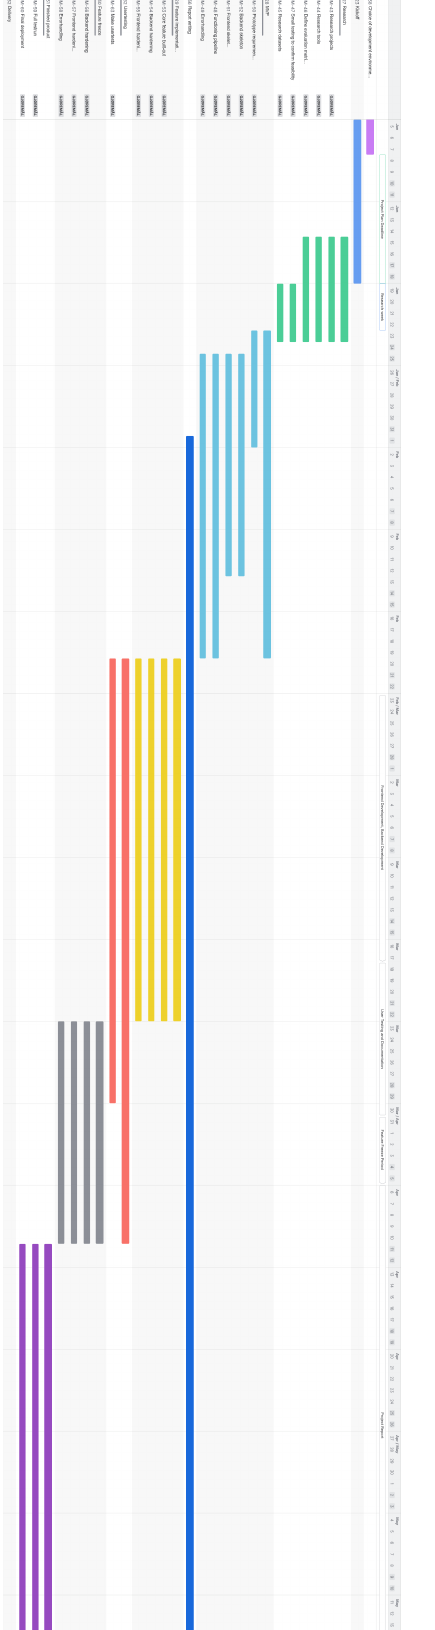
\includegraphics[height=0.75\textheight,keepaspectratio]{appendices/gantt_chart.png}
    \caption{Gantt chart for the project timeline.}
\end{figure}

\subsection{Milestones and Decision Points}

\begin{itemize}
    \item \textbf{Milestone 1, Choice of Development Environment (January 5 - January 7).} Decide between GitLab or GitHub, set up a Kanban board, assign roles, and handle other administrative tasks.
    \item \textbf{Milestone 2, Preliminary Project Deadline (January 8 - January 18).} Sign the group contract and complete the project plan.
    \item \textbf{Milestone 3, Research and Data Collection (January 15 - January 23).} Conduct research on similar projects and identify models that can be used for this project.
    \item \textbf{Milestone 4, Frontend and Backend prototype with destroy philosphy (January 23 - February 1.).} Test all tools for frontend and backend. Do work, but be ready to scrap and destroy progress that didnt work. Then we start over again and work on the real MVP with the gained experience.
    \item \textbf{Milestone 5, Frontend and Backend development (MVP) (January 23 - February 12).} Start frontend development and establish a pipeline for the backend.
    \item \textbf{Milestone 6, Backend Integration with Frontend (MVP) (February 12 - February 19).} Develop the backend and integrate it with the frontend.
    \item \textbf{Milestone 7, Feature implementations (February 19 - March 22).} Develop features to both frontend and backend/harden functionality.
    \item \textbf{Milestone 8, Project Testing, Documentation (February 20 - April 10).} Conduct user tests, double-check all existing tests and ensure documentation is complete where needed.
    \item \textbf{Milestone 9, Development Deadline (March 23 - April 10).} Feature freeze: no new additions, only refining existing work. Make the product as strong and reliable as possible with no more added features. Incorporate feedback from user tests and prepare everything for final submission.
    \item \textbf{Milestone 10, Project Report Writing (February 1 - May 16).} Begin writing the report and aim to complete it.
    \item \textbf{Milestone 11, Bachelor Project Deadline (May 16 - May 20).} Double-check that everything is ready for submission and polish the report.
\end{itemize}

\section{Gruppe kontrakt}

\begin{center}
    \Large\textbf{Gruppe konrakt - IDATG2901}\\[0.5em]
    An Hoang Chu, Henrik Weflen Gjermundsen, Karwan Shekhe\\[0.5em]
    Januar 2026
\end{center}

\subsection{Kontraktoverskrift}

Kontrakten gjelder for disse medlemmene:

\begin{itemize}
    \item An Hoang Chu
    \item Henrik Weflen Gjermundsen
    \item Karwan Shekhe
\end{itemize}

Kontrakten er gylding til 06.06.2026.

\subsection{Kommunikasjon og diskusjon}

\begin{itemize}
    \item Medlemmene skal kommunisere og diskutere sammen gjennom hele prosjektet, både fysisk og digitalt. Dersom noen blir syke eller er borte over lengre tid, skal dette kommuniseres tydelig, da det er viktig informasjon for resten av gruppen.
    \item Oppgave fordelig blir bestem gjennom diskusjon sammen blant gruppen, og blir tildelt på Jira sitt kanban. Denne diskusjonen bør skje under møtene og sprints. I tillegg blir det kommunisert på hvem som har kodet hva gjennom GitHub.
    \item Dersom det blir vanskelig å komme seg til en beslutning felles vil det være prosjektlederen som tar det endelige valget for gruppen.
\end{itemize}

\subsection{Ansvar og roller}

Rollene blir fordelt blant medlemmene etter at de har diskutert hvem de mener er egnet best for hva. Disse tre rollene blir prosjekt ansvarlig, scrum master og en dokument ansvarlig. Selv om det blir delt tre forskjellige roller innad gruppen, er enda alle tre utviklere.

\begin{itemize}
    \item Prosjekt ansvarlig tar ansvar for innholdet i prosjektet og hvordan det skal utføres. Passer også på at prosjektet går riktig vei og at kriterier blir møtt på god tid. Sørger for at det som blir pusha inn til Git er korrekt og holder øye på merges.
    \item Scrum master sørger for at møtereferater blir skrevet under hvert møte og setter opp møter og sprints. Holder øyet på at møtene ikke kræsjer med resten av medlemmene sine timeplaner og får møte i gang.
    \item Dokument ansvarlig passer på at dokumeneter er klare før fristende og at de er innafor kriteriene. Sørger for at alle formelle krav er oppfylt og dobbelsjekker kildene som brukes. Får alle medlemmer til å lese gjennom dokumentene slik at alle er enig om det som står der.
\end{itemize}

\subsection{Regler}

Under prosjekt perioden av gruppe kontrakten vil det være noen regler som bør bli holdt for å ha gode rutiner og bra arbeidsmoral.

\begin{itemize}
    \item Gruppe medlemmene skal samarbeide aktivt gjennom hele prosessen og dele kunnskap og ressurser innad gruppen.
    \item Oppgaver som blir tildelt må bli gjort og hver medlem bør ta iniativ til å gi seg selv flere oppgaver dersom de blir ferdig med sine opprinnelige oppgaver.
    \item Ikke lov til å gi seg selv flere enn tre issues.
    \item Reviews bør prioriteres, helst fullføre reviews før man går videre med sine issues.
    \item Det er obligatorisk å hjelpe en annen medlem når de spør om hjelp og sitter fast på noe.
    \item Alle skal passe på at de er oppdatert med arbeidet gjennom Jira og GitHub.
    \item Gruppe medlemmer er klare og vet når og hvor møtene skal holdes.
    \item Det skal være minst 30 timer med arbeid hver uke.
    \item Timer skal bli loggført.
\end{itemize}

\subsection{Møter}

Det vil være et første møte hvor gruppe medlemmer diskuterer innholdet i gruppe kontrakten og signerer det, samtidig fordeler roller og diskuterer fremtiden for gruppen. Det vil bli holdt daily scrums fra tirsdag til torsdag, hvor møtet på torsdag blir med oppdragsgiverene våres. I tillegg har vi en sprint review og retrospektiv hver mandag etter møtet med veileder. Møtene skal være fysisk på campus, men hvis to av tre medlemmer er syke kan det arrangeres en annen tid, dette bør kommuniseres på god tid.

Ved å signere dette dokumentet godtar du punktene over.

\vspace{2em}
\textbf{Signert av:}

\vspace{3em}
\begin{tabular}{p{0.3\textwidth}p{0.3\textwidth}p{0.3\textwidth}}
An Hoang Chu & Henrik Weflen Gjermundsen & Karwan Shekhe \\
\end{tabular}

\endgroup

% Full project hour tracking appendix generated from TimelisteBachelor2026.xlsx
% Recommended packages in the preamble:
% \usepackage{booktabs}
% \usepackage{longtable}
% \usepackage{array}
% \usepackage{graphicx}
% \usepackage{float}

\chapter{Project Hour Tracking}
\label{app:project-hour-tracking}
\raggedbottom

This appendix presents the project hour tracking maintained throughout the bachelor project. The hour list was used to document weekly work distribution across planning, meetings, documentation, programming, testing, research, figures, and administration. The appendix first presents a condensed overview of the total work distribution, followed by the complete weekly hour logs from the original spreadsheet.

\section{Condensed Overview}
\label{appendix:project-hour-tracking-overview}

\begin{table}[htbp]
\centering
\caption{Total registered project hours by group member.}
\label{tab:project-hours-member-total}
\begin{tabular}{lr}
\toprule
Group member & Total hours \\
\midrule
Hoang & 723 \\
Henrik & 674 \\
Karwan & 788.5 \\
\midrule
Total & 2185.5 \\
\bottomrule
\end{tabular}
\end{table}

\begin{table}[htbp]
\centering
\caption{Total registered project hours by activity category.}
\label{tab:project-hours-category-total}
\begin{tabular}{lr}
\toprule
Activity category & Total hours \\
\midrule
Programming & 729 \\
Report documentation & 579 \\
Planning and meetings & 309 \\
Research & 254 \\
Testing & 104 \\
Git and administration & 103.5 \\
Figures and diagrams & 63.5 \\
Code documentation & 43.5 \\
\midrule
Total & 2185.5 \\
\bottomrule
\end{tabular}
\end{table}

\begin{figure}[htbp]
    \centering
    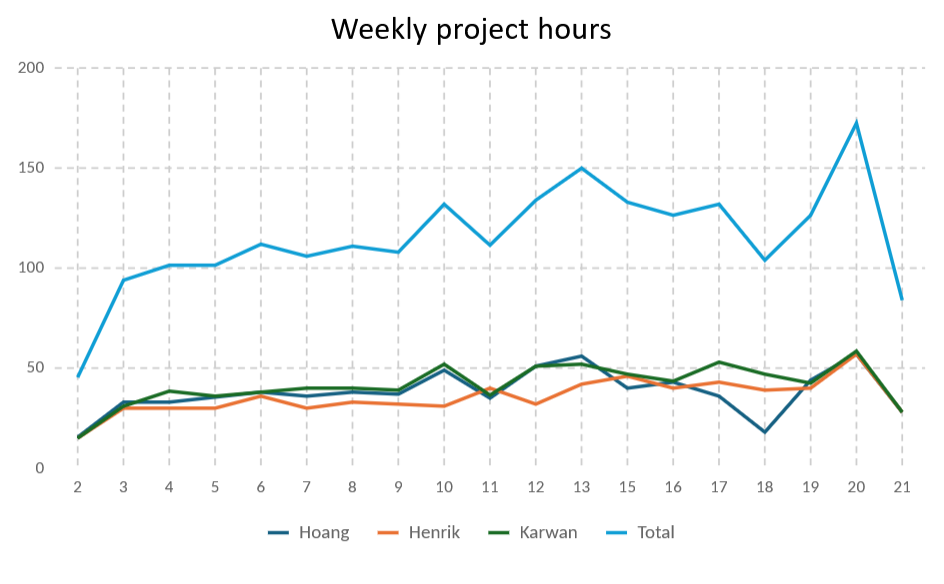
\includegraphics[width=0.85\textwidth]{figures/images/chapter-3/project_hours_weekly_summary_user_chart.png}
    \caption{Summary of registered project hours across the project period.}
    \label{fig:project-hours-weekly-summary}
\end{figure}

\begin{figure}[htbp]
    \centering
    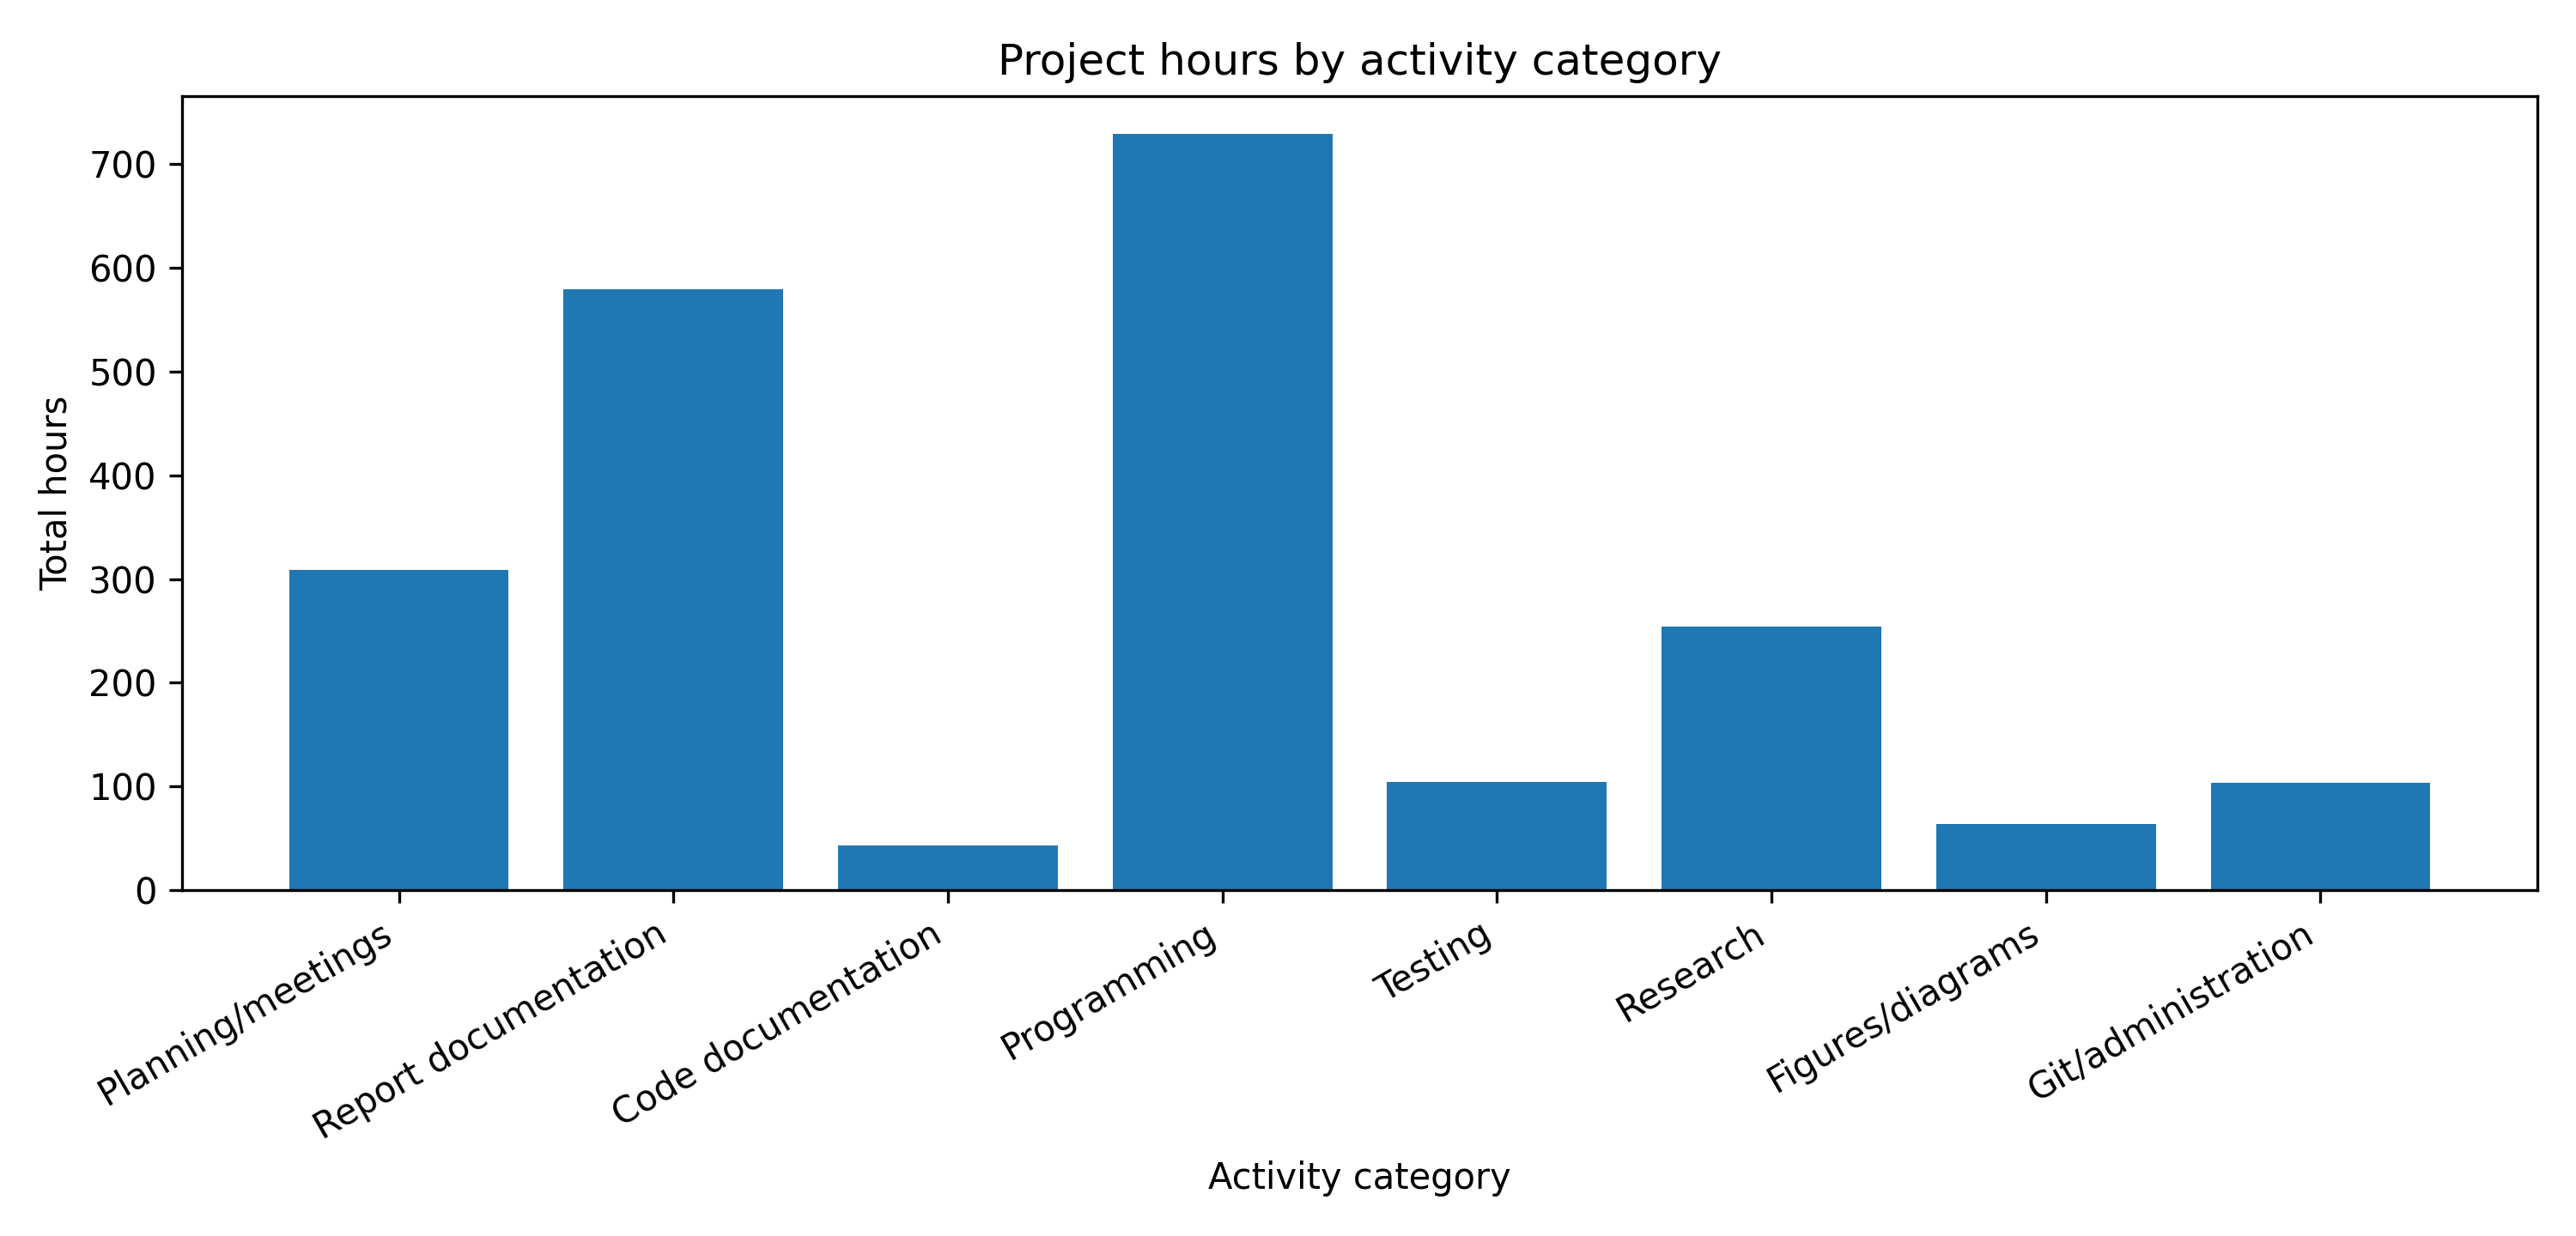
\includegraphics[width=0.80\textwidth]{figures/images/chapter-3/project_hours_category_summary.png}
    \caption{Distribution of registered project hours by activity category.}
    \label{fig:project-hours-category-summary}
\end{figure}

\begin{longtable}{lrrrr}
\caption{Weekly registered project hours by group member.}
\label{tab:project-hours-weekly-overview}\\
\toprule
Week & Hoang & Henrik & Karwan & Total \\
\midrule
\endfirsthead
\toprule
Week & Hoang & Henrik & Karwan & Total \\
\midrule
\endhead
Uke2 & 15.5 & 15 & 15 & 45.5 \\
Uke3 & 33 & 30 & 31 & 94 \\
Uke4 & 33 & 30 & 38.5 & 101.5 \\
Uke5 & 35.5 & 30 & 36 & 101.5 \\
Uke6 & 38 & 36 & 38 & 112 \\
Uke7 & 36 & 30 & 40 & 106 \\
Uke8 & 38 & 33 & 40 & 111 \\
Uke9 & 37 & 32 & 39 & 108 \\
Uke10 & 49 & 31 & 52 & 132 \\
Uke11 & 35 & 40 & 36.5 & 111.5 \\
Uke12 & 51 & 32 & 51 & 134 \\
Uke13 & 56 & 42 & 52 & 150 \\
Uke15 & 40 & 46 & 47 & 133 \\
Uke16 & 43 & 40 & 43.5 & 126.5 \\
Uke17 & 36 & 43 & 53 & 132 \\
Uke18 & 18 & 39 & 47 & 104 \\
Uke19 & 44 & 40 & 42.5 & 126.5 \\
Uke20 & 57 & 57 & 58.5 & 172.5 \\
Uke21 & 28 & 28 & 28 & 84 \\
\midrule
Total & 723 & 674 & 788.5 & 2185.5 \\
\bottomrule
\end{longtable}

\section{Complete Weekly Hour Logs}
\label{appendix:project-hour-tracking-complete}

The following tables reproduce the complete weekly hour logs from the project hour list. Each week includes the registered hours by activity category and group member. When the spreadsheet included written comments, these are included below the corresponding weekly hour table.

\subsection{Uke2}

\begin{table}[H]
\centering
\small
\caption{Registered hours for Uke2.}
\label{tab:project-hours-uke2}
\begin{tabular}{lrrrr}
\toprule
Activity & Hoang & Henrik & Karwan & Total \\
\midrule
Møter & 4 & 4 & 4 & 12 \\
Dokumentasjon - Rapport & 5 & 6 & 5 & 16 \\
Dokumentasjon - Kode & 0 & 0 & 0 & 0 \\
Programmering & 0 & 0 & 0 & 0 \\
Testing & 0 & 0 & 0 & 0 \\
Forskning & 4 & 2 & 3 & 9 \\
Figurer og diagrammer & 0.5 & 1.5 & 1 & 3 \\
Git / Administrasjon & 2 & 1.5 & 2 & 5.5 \\
\midrule
Total & 15.5 & 15 & 15 & 45.5 \\
\bottomrule
\end{tabular}
\end{table}

\begin{longtable}{p{0.20\textwidth}p{0.72\textwidth}}
\caption{Written activity notes for Uke2.}\\
\toprule
Entry & Notes \\
\midrule
\endfirsthead
\toprule
Entry & Notes \\
\midrule
\endhead
Hoang & Satte opp GitLab Kanban tavle og excel dokumentet. \newline Tok kontakt med OsloSkolen for mulig samarbeid. \newline Satte opp gruppe kontrakt og fikk signaturer. \newline Ansvar for kapittel en og tre for prosjektplanen. \\
\addlinespace
Henrik & Har skrevet punkt 4 om planlegging, oppfølging og rapportering. Har skrevet møtereferater og satt opp online møter. Har laget kanaler hvor vi kan snakke sammen og dele felles dokumenter/organisere ting vi har diskutert etter tema slik at vi lett kan finne fram og være oppdatert. Har utforsket teori om oppgaven. \\
\addlinespace
Karwan & Forskning: Forbredelse ved å lese tidligere bachleor oppgaver. Møter: Henvend til møtereferatene fra uke 2. Rapportering: Skrive "Organisering og Kvalitetssikring" og analysere risiko. Kontakte ulike bedrifter for mulige bachleor oppgaver. \\
\addlinespace
\bottomrule
\end{longtable}

\subsection{Uke3}

\begin{table}[H]
\centering
\small
\caption{Registered hours for Uke3.}
\label{tab:project-hours-uke3}
\begin{tabular}{lrrrr}
\toprule
Activity & Hoang & Henrik & Karwan & Total \\
\midrule
Møter & 7 & 8 & 7 & 22 \\
Dokumentasjon - Rapport & 9 & 6 & 7 & 22 \\
Dokumentasjon - Kode & 0 & 0 & 0 & 0 \\
Programmering & 0 & 0 & 0 & 0 \\
Testing & 0 & 0 & 0 & 0 \\
Forskning & 10 & 6 & 14 & 30 \\
Figurer og diagrammer & 1 & 6 & 2 & 9 \\
Git / Administrasjon & 6 & 4 & 1 & 11 \\
\midrule
Total & 33 & 30 & 31 & 94 \\
\bottomrule
\end{tabular}
\end{table}

\begin{longtable}{p{0.20\textwidth}p{0.72\textwidth}}
\caption{Written activity notes for Uke3.}\\
\toprule
Entry & Notes \\
\midrule
\endfirsthead
\toprule
Entry & Notes \\
\midrule
\endhead
Hoang & Bearbeidet prosjektplanen, og har sett på en del research angående sladding av sensitiv informasjon på bilder, hvordan andre modeller har gjort det kontra våres potensiell løsnign. Har også gjort en del research om react rammeverket og hvordan det brukes for å lage nettsider, I tillegg til å eksperimentere med rammeverket. Har også satt opp GitHub og Jira, og vurdert hvilken kanban tavle som er best (kollektivt). Opprettet frontend prosjektet og initialisert til GitHub. \\
\addlinespace
Henrik & Jobbet videre med prosjektplanen. Skrevet møtereferater og notert på møter. Oppsummert møter og vært scrum ansvarlig. Kommet på ideer til løsninger. Bidrat til spørsmål til oppdragsgiver/rådgiver. Laget Gantt skjema og kommet på plan for prosjektets tidslinje. Hjulpet med å komme på løsning til administrasjon og sette opp Jira. \\
\addlinespace
Karwan & Bruke tid på å se etter eksisterende løsninger innen ansiktdjenskjenning og ansiktsdetection. Se etter modeller som kan brukes i prosjektet. Lese teori innen maskin læring. Teste disse ulike eksisterende løsningene på python og se om det er noe å ta med. Pusse opp omfang delen i prosjekt rapporten. Fikse Wiki page for GitHub. \\
\addlinespace
\bottomrule
\end{longtable}

\subsection{Uke4}

\begin{table}[H]
\centering
\small
\caption{Registered hours for Uke4.}
\label{tab:project-hours-uke4}
\begin{tabular}{lrrrr}
\toprule
Activity & Hoang & Henrik & Karwan & Total \\
\midrule
Møter & 7 & 8 & 7 & 22 \\
Dokumentasjon - Rapport & 4 & 5 & 4 & 13 \\
Dokumentasjon - Kode & 0 & 0 & 1 & 1 \\
Programmering & 17 & 0 & 20 & 37 \\
Testing & 0 & 0 & 2 & 2 \\
Forskning & 3 & 10 & 4 & 17 \\
Figurer og diagrammer & 0 & 2 & 0.5 & 2.5 \\
Git / Administrasjon & 2 & 5 & 0 & 7 \\
\midrule
Total & 33 & 30 & 38.5 & 101.5 \\
\bottomrule
\end{tabular}
\end{table}

\begin{longtable}{p{0.20\textwidth}p{0.72\textwidth}}
\caption{Written activity notes for Uke4.}\\
\toprule
Entry & Notes \\
\midrule
\endfirsthead
\toprule
Entry & Notes \\
\midrule
\endhead
Hoang & Brukt meste av tiden til å utvikle en prototype som skal bli kastet på react + vite i tillegg til litt research om best practices innen for dem. Fått til en enkel nettside med enkel redigering. Redigert litt på prosjektplanen etter tilbakemelding fra veileder og passe på at språket er mer konsistent. \\
\addlinespace
Henrik & Ferdigstillte prosjektrapport. Fant state of the art av image preprocessing for facedetection, object detection og character detection. Researchet hva som menes med sensitiv informasjon/hva som brukes i praksis. Skrev møtereferater, passet på at scrum ble fulgt. \\
\addlinespace
Karwan & Research innen face recognition og face detection. Finne modeller som gir gode resultater. Testing for å gjøre disse modellene bedre. Vi valgte RetinaFace for å finne ansikter i bilder, for den er den største modellen og som gir veldig gode resultater, både av små ansikter (distanse ) og gruppe bilder. Retina er dårlig på å finne ansikter som ikke vises fult (f.eks hjelm, maske, osv), la til augmentasjion + occulation for å gjøre modellen bedre. Bruker YOLO for å finne fulle kropper og ikke bare ansikter. Evaluere modellene, sammenligne fine tuned modell med base modellen. \\
\addlinespace
\bottomrule
\end{longtable}

\subsection{Uke5}

\begin{table}[H]
\centering
\small
\caption{Registered hours for Uke5.}
\label{tab:project-hours-uke5}
\begin{tabular}{lrrrr}
\toprule
Activity & Hoang & Henrik & Karwan & Total \\
\midrule
Møter & 5 & 6 & 5 & 16 \\
Dokumentasjon - Rapport & 4 & 1 & 1 & 6 \\
Dokumentasjon - Kode & 3 & 0 & 1 & 4 \\
Programmering - Front & 18 & 0 & 0 & 18 \\
Programmering - Back & 0 & 7 & 19 & 26 \\
Testing & 1 & 1 & 1 & 3 \\
Forskning & 2 & 13 & 8 & 23 \\
Figurer og diagrammer & 0.5 & 1 & 0 & 1.5 \\
Git / Administrasjon & 2 & 1 & 1 & 4 \\
\midrule
Total & 35.5 & 30 & 36 & 101.5 \\
\bottomrule
\end{tabular}
\end{table}

\begin{longtable}{p{0.20\textwidth}p{0.72\textwidth}}
\caption{Written activity notes for Uke5.}\\
\toprule
Entry & Notes \\
\midrule
\endfirsthead
\toprule
Entry & Notes \\
\midrule
\endhead
Hoang & Skrev siste endringer (GDPR og regler) på prosjektplan etter møte med oppdragsgiver, samtidig som tankekartet ble revidert. La til manuell sladding i frontend samtidig enkle funksjonalitet som å laste ned filen og zoome in og ut på bildet. Protoypen ble refaktorert og satt inn i MVP repo. Dokumentasjon for klassene ble lagt til, kompleks logikk fikk kommentarer. Sett bittelitt på hvordan GitHub Actions fungerer og satt det opp. \\
\addlinespace
Henrik & Researchet/laget og testet kode for preprocessing av bilder opp mot retinaface-modellen. Hvilke threshholds/hva slags preprocessing gjør at modellen klarer å finne flest ansikter i en folkemengde. Hva fungerer best på bilder med forskjellig stø. Hva vil være beste metode med tanke på tid modellen bruker. Dersom vi skal legge til tekst i framtiden, hva slags preprocessing gjøres for å detektere områder der tekst mest sannsynlig ligger i bildet. Skrevet på rapport. Endret på Gannt skjema. \\
\addlinespace
Karwan & Finpusse prosjektplan rapporten. Gå gjennom for å bekrefte den før levering. Implementere pipeline for backend slik at den kan senere bli brukt av frontend. Implementere API, og ulike endepunkter for å sende informasjon. Fine-tune retinaface modellen for å se om vi kan gjøre den bedre enn base modellen. \\
\addlinespace
\bottomrule
\end{longtable}

\subsection{Uke6}

\begin{table}[H]
\centering
\small
\caption{Registered hours for Uke6.}
\label{tab:project-hours-uke6}
\begin{tabular}{lrrrr}
\toprule
Activity & Hoang & Henrik & Karwan & Total \\
\midrule
Oppgave Tema & 0 & 0 & 0 & 0 \\
Planlegging/Møter & 5 & 6 & 5 & 16 \\
Dokumentasjon - Rapport & 0 & 6 & 0 & 6 \\
Dokumentasjon - Kode & 3 & 0 & 2 & 5 \\
Programmering - Front & 26 & 0 & 2 & 28 \\
Programmering - Back & 0 & 13 & 25 & 38 \\
Testing & 0 & 0 & 1 & 1 \\
Forskning & 2 & 10 & 2 & 14 \\
Figurer og diagrammer & 0 & 0 & 0 & 0 \\
Git / Administrasjon & 2 & 1 & 1 & 4 \\
\midrule
Total & 38 & 36 & 38 & 112 \\
\bottomrule
\end{tabular}
\end{table}

\begin{longtable}{p{0.20\textwidth}p{0.72\textwidth}}
\caption{Written activity notes for Uke6.}\\
\toprule
Entry & Notes \\
\midrule
\endfirsthead
\toprule
Entry & Notes \\
\midrule
\endhead
Hoang & Riktig skalering på knapper og komponenter avhengig av vindu størrelse er nå implementert. Lagt til andre UI/UX elementer som kan hjelpe bruker opplevelsen. PDF er nå redigerbar. Prøvd å refaktorere koden, men må jobbes mer med. Har satt opp inndeling for prosjekt rapporten. \\
\addlinespace
Henrik & Har jobbet med segmentation av personer i bildene i backend. Har gjort forskning på gdpr, state of the art og så vidt begynt på rapporten for kapittel 2. \\
\addlinespace
Karwan & Optimalisere hastigheten til redaction av ansikter, for redaction var unødvendig treig. Gi mulighet til brukeren slik at de kan velge ut hva slags ansikter de ikke vil redacte. Gjøre anonymisering sterkere. Bruke Go som offisiel språk for API. Rydde og refaktorisere koden slik at det er ryddig, legge til dokumentasjon. \\
\addlinespace
\bottomrule
\end{longtable}

\subsection{Uke7}

\begin{table}[H]
\centering
\small
\caption{Registered hours for Uke7.}
\label{tab:project-hours-uke7}
\begin{tabular}{lrrrr}
\toprule
Activity & Hoang & Henrik & Karwan & Total \\
\midrule
Planlegging/Møter & 5 & 6 & 5 & 16 \\
Dokumentasjon - Rapport & 14 & 8 & 0 & 22 \\
Dokumentasjon - Kode & 0 & 0 & 1 & 1 \\
Programmering - Front & 2 & 0 & 10 & 12 \\
Programmering - Back & 0 & 0 & 12 & 12 \\
Testing & 0 & 0 & 5 & 5 \\
Forskning & 9 & 14 & 5 & 28 \\
Figurer og diagrammer & 2 & 0 & 0 & 2 \\
Git / Administrasjon & 4 & 2 & 2 & 8 \\
\midrule
Total & 36 & 30 & 40 & 106 \\
\bottomrule
\end{tabular}
\end{table}

\begin{longtable}{p{0.20\textwidth}p{0.72\textwidth}}
\caption{Written activity notes for Uke7.}\\
\toprule
Entry & Notes \\
\midrule
\endfirsthead
\toprule
Entry & Notes \\
\midrule
\endhead
Hoang & Inndelte kapitlene enda mer I overleaf for å lage grov oversikt over hva som skal med, basert på tidligere bachelor oppgaver. Startet med første chapter for bachelor oppgavene, altså om oppgavebeskrivelsen, mål, rammer, osv. Gjorde en del research om lignende oppgaver og om modeller som kan brukes for tekst og om lisenser som trengs. I tillegg lest en del bachelor oppgaver for å få helhetelig bildet på hvordan våres skal se ut. \\
\addlinespace
Henrik & Har researchet gdpr, state of art, begynt på rapporten og sett på mulige løsninger for videreutvikling av koden. \\
\addlinespace
Karwan & Refaktorere koden til frontend og backend. Ridde opp dokumentasjoner, dele opp koden. Refaktorere mappe struktur. Fikse bugs, blant annent som synkronisere manuel redaction med automatisk redaction. Gjøre hastigheten til redaction bedre. Legge til CRAFT (tekst deteksjon) til backend og koble den til frontend. Forskning innen ulike modeller for tekstdeteksjon innen bilder. \\
\addlinespace
\bottomrule
\end{longtable}

\subsection{Uke8}

\begin{table}[H]
\centering
\small
\caption{Registered hours for Uke8.}
\label{tab:project-hours-uke8}
\begin{tabular}{lrrrr}
\toprule
Activity & Hoang & Henrik & Karwan & Total \\
\midrule
Planlegging/Møter & 5 & 6 & 5 & 16 \\
Dokumentasjon - Rapport & 6 & 0 & 0 & 6 \\
Dokumentasjon - Kode & 1 & 0 & 1 & 2 \\
Programmering - Front & 14 & 10 & 2 & 26 \\
Programmering - Back & 0 & 8 & 23 & 31 \\
Programmering - Bugs & 5 & 2 & 1 & 8 \\
Testing & 0 & 0 & 3 & 3 \\
Forskning & 4 & 5 & 3 & 12 \\
Figurer og diagrammer & 0 & 0 & 1 & 1 \\
Git / Administrasjon & 3 & 2 & 1 & 6 \\
\midrule
Total & 38 & 33 & 40 & 111 \\
\bottomrule
\end{tabular}
\end{table}

\begin{longtable}{p{0.20\textwidth}p{0.72\textwidth}}
\caption{Written activity notes for Uke8.}\\
\toprule
Entry & Notes \\
\midrule
\endfirsthead
\toprule
Entry & Notes \\
\midrule
\endhead
Hoang & Prøvd å ta litt kontakt med ulike potenseille bruketestere som for eksempel fra NRK eller VG. Brukt tid på å legge til bruke innstillinger I applikasjonen vår, I tillegg til å fikse noen bugs. Har satt opp overleaf dokumentet etter ntnu sine standarder og holder på å overføre tekst fra den gamle. Gjort litt mer forksning på the state of art. \\
\addlinespace
Henrik & Jobbet med downscaling methods i backend. Fikset terms of service i frontend. Lagde to forskjellige brukertester, en tilpasset testing for funksjonalitet og en for UI. \\
\addlinespace
Karwan & Fjerne PDF støtte pga ikke lenger behov, forenkle frontend for kunn bilde støtte. Teste alle ende punkter (redact\&detect) og sørge for at de fungerer. Dekke så mye av backend koden som mulig med unit testing. Legge til script for å starte frontend og backend enkelt samtidig (loklat). Contrainerize backend med docker. Fikse Google Cloud Run for å kunne deploye applikasjonen. Legge til dokumenatison i koden. Evaluere retinaface modelene (resnet50 og mobilnet\_25) for rapport og prøve å fine tune den. \\
\addlinespace
\bottomrule
\end{longtable}

\subsection{Uke9}

\begin{table}[H]
\centering
\small
\caption{Registered hours for Uke9.}
\label{tab:project-hours-uke9}
\begin{tabular}{lrrrr}
\toprule
Activity & Hoang & Henrik & Karwan & Total \\
\midrule
Planlegging/Møter & 5 & 6 & 5 & 16 \\
Dokumentasjon - Rapport & 3 & 0 & 0 & 3 \\
Dokumentasjon - Kode & 1 & 0 & 1 & 2 \\
Programmering - Front & 21 & 0 & 10 & 31 \\
Programmering - Back & 0 & 7 & 15 & 22 \\
Programmering - Bugs & 0 & 0 & 5 & 5 \\
Testing & 2 & 9 & 1 & 12 \\
Forskning & 4 & 4 & 1 & 9 \\
Figurer og diagrammer & 0 & 3 & 0 & 3 \\
Git / Administrasjon & 1 & 3 & 1 & 5 \\
\midrule
Total & 37 & 32 & 39 & 108 \\
\bottomrule
\end{tabular}
\end{table}

\begin{longtable}{p{0.20\textwidth}p{0.72\textwidth}}
\caption{Written activity notes for Uke9.}\\
\toprule
Entry & Notes \\
\midrule
\endfirsthead
\toprule
Entry & Notes \\
\midrule
\endhead
Hoang & La til ulike UI/UX funksjonaliteter som for eksempel farge endring, filtere og brukerpreferanser. Har startet med å legge til noe support for video og videoformatering. Gjort research på hvordan tidligere prosjekter/andre bedrifter og firmaer og gjort denne løsningen. Forbedret biter fra chapter 1 fra det gamle overleaf dokumentet. Har også sett på standarder innen for testing og hvordan testing skal være, i tillegg til å lage nye test filer og oppdatere den gamle test filen. \\
\addlinespace
Henrik & Tok kontakt med firmaer for brukertesting. Lagde funksjon for å få bounding boxes fra video ved bruk av tracking. Testet alle mulige API calls lokalt og via nettsiden, fra powershell og inspector tools, for å se hvor performance går tapt. Samlet dataen og lagde simple tabeller for dette. Fikk en oversikt over pipeline og hva som gjør at vi mister performance underveis der (benchmarking). \\
\addlinespace
Karwan & Fikse bugger fra applikasjonen. Utforske andre tekst deteksjons modeller som er bedre enn CRAFT. Bytte teks deteksjon fra CRAFT til PaddleOCR. Oppdatere tester. Legge til tekst analyse etter tekst deteksjon for å kunne filtrere de ut (om det er noe sensetiv info., som tlf. nummer, bil skylt, post nummer, osv.). Koble filtrering funsksjonalitet til frontend. Refaktorere frontend. Legge til QR-Bar -Detection. \\
\addlinespace
\bottomrule
\end{longtable}

\subsection{Uke10}

\begin{table}[H]
\centering
\small
\caption{Registered hours for Uke10.}
\label{tab:project-hours-uke10}
\begin{tabular}{lrrrr}
\toprule
Activity & Hoang & Henrik & Karwan & Total \\
\midrule
Planlegging/Møter & 5 & 6 & 5 & 16 \\
Dokumentasjon - Rapport & 11 & 0 & 12 & 23 \\
Dokumentasjon - Kode & 1 & 0 & 1 & 2 \\
Programmering - Front & 3 & 0 & 2 & 5 \\
Programmering - Back & 0 & 13 & 10 & 23 \\
Programmering - Bugs & 11 & 0 & 10 & 21 \\
Testing & 6 & 4 & 2 & 12 \\
Forskning & 8 & 0 & 5 & 13 \\
Figurer og diagrammer & 1 & 0 & 4 & 5 \\
Git / Administrasjon & 3 & 8 & 1 & 12 \\
\midrule
Total & 49 & 31 & 52 & 132 \\
\bottomrule
\end{tabular}
\end{table}

\begin{longtable}{p{0.20\textwidth}p{0.72\textwidth}}
\caption{Written activity notes for Uke10.}\\
\toprule
Entry & Notes \\
\midrule
\endfirsthead
\toprule
Entry & Notes \\
\midrule
\endhead
Hoang & Testere for utils og hooks samtidig integrasjons tests ble laget. Ordnet mer på overleaf dokumentet sin fil struktur og pakker, samtidig ble det hentet frem/laget nye figurer for kapitell 6. Har startet å skrive på kapittel 6 og kapittel 1 har blitt revidert utifra tilbakemleding fra veileder. Prøvd å fikse fleste bugs fra kanalen vår og lagt til en drag feature for når man er zoomed langt inn på canvas. \\
\addlinespace
Henrik & Har hold kontakt med bedrifter for brukertesting. Har fått video til å fungere med redact, og endret struktur og logikk slik at det skal være lett å koble det opp med siden vår. \\
\addlinespace
Karwan & Utforsket ulike modeller vi kan finetune for licensplate og barcode deteksjon. YOLOX var den som fylte alle kravene (lisens, gratis og bra). Samlet inn data for barcode, brukte mye tid på å finne dataset, kombinerte fra ulike kilder. Deretter finpusset (fjerne duplikater, bilder uten labels, osv) og splittet jeg datasettet og gjorde det klar for trening. Trente modellen og andre modeller med ulike parametere, samlet data også lagde jeg figurer for evalueringer. Brukte disse da til rapporten, og skrev i kappitel 8 og 13. Implemnterte beste modellen for barcode inn i systemet, og debugget til alt fungerte. \\
\addlinespace
\bottomrule
\end{longtable}

\subsection{Uke11}

\begin{table}[H]
\centering
\small
\caption{Registered hours for Uke11.}
\label{tab:project-hours-uke11}
\begin{tabular}{lrrrr}
\toprule
Activity & Hoang & Henrik & Karwan & Total \\
\midrule
Planlegging/Møter & 8 & 9 & 5 & 22 \\
Dokumentasjon - Rapport & 0 & 0 & 2 & 2 \\
Dokumentasjon - Kode & 1 & 0 & 0.5 & 1.5 \\
Programmering - Front & 4 & 0 & 0 & 4 \\
Programmering - Back & 0 & 8 & 15 & 23 \\
Programmering - Bugs & 10 & 0 & 3 & 13 \\
Testing & 1 & 0 & 2 & 3 \\
Forskning & 5 & 15 & 2 & 22 \\
Figurer og diagrammer & 0 & 0 & 2 & 2 \\
Git / Administrasjon & 6 & 8 & 5 & 19 \\
\midrule
Total & 35 & 40 & 36.5 & 111.5 \\
\bottomrule
\end{tabular}
\end{table}

\begin{longtable}{p{0.20\textwidth}p{0.72\textwidth}}
\caption{Written activity notes for Uke11.}\\
\toprule
Entry & Notes \\
\midrule
\endfirsthead
\toprule
Entry & Notes \\
\midrule
\endhead
Hoang & Forbrede til møte og jobbet med å få til en fungerende versjon for deployment til møte med skan kontroll. Gjorde litt forskning på metadata og hvordan undersøke om et bildet er legitimt eller laget av kunstig intelligens. Etter rell behov. Også litt research på hvordan man får maksimal utbytte av brukertesting. \\
\addlinespace
Henrik & Forbrede til møte med skan kontroll og delta på møtet. Jobbet også med videoimplementasjon og gjorde research på kalman filter og annet video tracking muligheter. \\
\addlinespace
Karwan & Jobbet med YOLOX/data module og requrments. Trente YOLOX-S license plate deteksjons modell. Evaluerte modellen, lagde oversiktlig evaluerings grafer og skrev resultat analyse for rapporten. Implementerte modellen inn i SafeVision backend systemet. Fikset Docker, Cloud Run, model preload. Fikse på CI/CD problemer (modeller blir ikke lastet til google cloude). Fikset bounding boxes for skilt ved scaling mismatch. \\
\addlinespace
\bottomrule
\end{longtable}

\subsection{Uke12}

\begin{table}[H]
\centering
\small
\caption{Registered hours for Uke12.}
\label{tab:project-hours-uke12}
\begin{tabular}{lrrrr}
\toprule
Activity & Hoang & Henrik & Karwan & Total \\
\midrule
Planlegging/Møter & 7 & 8 & 5 & 20 \\
Dokumentasjon - Rapport & 9 & 0 & 0 & 9 \\
Dokumentasjon - Kode & 1 & 0 & 5 & 6 \\
Programmering - Front & 18 & 0 & 2 & 20 \\
Programmering - Back & 0 & 20 & 25 & 45 \\
Programmering - Bugs & 5 & 0 & 5 & 10 \\
Testing & 2 & 0 & 3 & 5 \\
Forskning & 5 & 3 & 1 & 9 \\
Figurer og diagrammer & 3 & 0 & 0 & 3 \\
Git / Administrasjon & 1 & 1 & 5 & 7 \\
\midrule
Total & 51 & 32 & 51 & 134 \\
\bottomrule
\end{tabular}
\end{table}

\begin{longtable}{p{0.20\textwidth}p{0.72\textwidth}}
\caption{Written activity notes for Uke12.}\\
\toprule
Entry & Notes \\
\midrule
\endfirsthead
\toprule
Entry & Notes \\
\midrule
\endhead
Hoang & Møte med Thomas Berg Fjellestad som er studieprogramleder og universitetslektor ga informasjon om hvordan få mer ut av brukertesting og annet teori rundt det. I tillegg litt feedback på UI/UX designet vårt. Prøvde å få til metadata inn til frontenden, men bestemte for å kutte det ut. La til tooltips og labels for å gjøre det lettere å navigere rundt UI/UX. Har også gjort om ID fra number til Strings. Ny funksjonalitet er høyreklikk og highlights på bokser for å indikere at de er selected. Skrevet noe i chapter 3 i rapporten. Og revidert litt utifra tilbakemelding fra veileder. \\
\addlinespace
Henrik & Jobbet med videoimplementasjon, forbredet og deltok på møte om brukertesting og UI design \\
\addlinespace
Karwan & La til concurrency i detect/redact pipelines. Utvidet detection pipeline med objekt-detection, categories og entities. Fikset redaction box masking og single-pass anonymization. Oppdaterte dokumentasjon. Rettet CI- og ruff-feil. \\
\addlinespace
\bottomrule
\end{longtable}

\subsection{Uke13}

\begin{table}[H]
\centering
\small
\caption{Registered hours for Uke13.}
\label{tab:project-hours-uke13}
\begin{tabular}{lrrrr}
\toprule
Activity & Hoang & Henrik & Karwan & Total \\
\midrule
Planlegging/Møter & 5 & 6 & 5 & 16 \\
Dokumentasjon - Rapport & 25 & 6 & 0 & 31 \\
Dokumentasjon - Kode & 1 & 1 & 2 & 4 \\
Programmering - Front & 12 & 4 & 8 & 24 \\
Programmering - Back & 0 & 12 & 25 & 37 \\
Programmering - Bugs & 4 & 4 & 4 & 12 \\
Testing & 2 & 5 & 2 & 9 \\
Forskning & 3 & 3 & 5 & 11 \\
Figurer og diagrammer & 3 & 0 & 0 & 3 \\
Git / Administrasjon & 1 & 1 & 1 & 3 \\
\midrule
Total & 56 & 42 & 52 & 150 \\
\bottomrule
\end{tabular}
\end{table}

\begin{longtable}{p{0.20\textwidth}p{0.72\textwidth}}
\caption{Written activity notes for Uke13.}\\
\toprule
Entry & Notes \\
\midrule
\endfirsthead
\toprule
Entry & Notes \\
\midrule
\endhead
Hoang & Jobbet enda mer med rapport, skrevet ferdig kapittel 6 (ui design) inkludert figurer og noe på 7 (teknologi) og 8 (implementasjon) om frontend. I tillegg ble det gjort en del refaktorering med filter funksjonalitet og entitets typer. \\
\addlinespace
Henrik & Jobbet videre med videoimplementasjon og backendlogikk for video. Rettet på problemer knyttet til videoredigering og modeller. Deltok på møter om scope og video. Brukte tid på førsteutkastet av rapporten (kapittel 2 og 3) \\
\addlinespace
Karwan & La til MobileSAM-kildekode. Forbedret MobileSAM redaction med cropped ROI-segmentering. Fikset video redaction med segmentation. Fikset frontend/backend mapping for detection requests. Fjernet unødvendige debug logs.\newline Løste merge conflicts og skrev patch notes. \\
\addlinespace
\bottomrule
\end{longtable}

\subsection{Uke15}

\begin{table}[H]
\centering
\small
\caption{Registered hours for Uke15.}
\label{tab:project-hours-uke15}
\begin{tabular}{lrrrr}
\toprule
Activity & Hoang & Henrik & Karwan & Total \\
\midrule
Planlegging/Møter & 5 & 6 & 5 & 16 \\
Dokumentasjon - Rapport & 5 & 14 & 15 & 34 \\
Dokumentasjon - Kode & 1 & 1 & 0 & 2 \\
Programmering - Front & 12 & 10 & 0 & 22 \\
Programmering - Back & 0 & 5 & 14 & 19 \\
Programmering - Bugs & 3 & 2 & 2 & 7 \\
Testing & 3 & 3 & 2 & 8 \\
Forskning & 10 & 3 & 3 & 16 \\
Figurer og diagrammer & 0 & 1 & 5 & 6 \\
Git / Administrasjon & 1 & 1 & 1 & 3 \\
\midrule
Total & 40 & 46 & 47 & 133 \\
\bottomrule
\end{tabular}
\end{table}

\begin{longtable}{p{0.20\textwidth}p{0.72\textwidth}}
\caption{Written activity notes for Uke15.}\\
\toprule
Entry & Notes \\
\midrule
\endfirsthead
\toprule
Entry & Notes \\
\midrule
\endhead
Hoang & Skrev ferdig kapittel 11 bærekraft og gjorde research på SuSAF modellen, og har prøvd å lage dataset for PDF417, noe vi bestemte oss for at ikke var verdt det med tanke på tiden vi har. Hadde noen brukertestere med medstudenter. Fikset en bug med at video ikke kunne spilles når manuell verktøy var på, og refaktorerte mye av video koden. I tillegg ble det implementert små QoL funksjonalitet som å avrbyte en prosess mid process og rekkefølgen på knappene . \\
\addlinespace
Henrik & Skrev ferdig kapittel 2 og 3. Ferdigstilte automatisk tracking for video. Både detection og redaction fungerer på siden og man får opp resultat og kan laste ned. \\
\addlinespace
Karwan & Fikset category types mellom backend og frontend. Legge til inpaint som et alternativ redaksjons metode\newline Fikset inpaint prompt. Begyne skrive implementasjons kap, og resultat kap. \\
\addlinespace
\bottomrule
\end{longtable}

\subsection{Uke16}

\begin{table}[H]
\centering
\small
\caption{Registered hours for Uke16.}
\label{tab:project-hours-uke16}
\begin{tabular}{lrrrr}
\toprule
Activity & Hoang & Henrik & Karwan & Total \\
\midrule
Planlegging/Møter & 5 & 6 & 5 & 16 \\
Dokumentasjon - Rapport & 8 & 11 & 10 & 29 \\
Dokumentasjon - Kode & 1 & 1 & 1 & 3 \\
Programmering - Front & 10 & 2 & 0 & 12 \\
Programmering - Back & 0 & 8 & 15 & 23 \\
Programmering - Bugs & 9 & 2 & 0.5 & 11.5 \\
Testing & 0 & 5 & 1 & 6 \\
Forskning & 10 & 3 & 6 & 19 \\
Figurer og diagrammer & 0 & 1 & 4 & 5 \\
Git / Administrasjon & 0 & 1 & 1 & 2 \\
\midrule
Total & 43 & 40 & 43.5 & 126.5 \\
\bottomrule
\end{tabular}
\end{table}

\begin{longtable}{p{0.20\textwidth}p{0.72\textwidth}}
\caption{Written activity notes for Uke16.}\\
\toprule
Entry & Notes \\
\midrule
\endfirsthead
\toprule
Entry & Notes \\
\midrule
\endhead
Hoang & Startet å skrive noe for abstract og summary. En QoL feature ble lagt til, høyre klikk for å copy and paste boxer. Fil nøkler er nå "kryptert" i lokal database. I tillegg ble end del bugs i frontend fjernet. Til slutt så ble det gjort noen ekstra eksperimenter fra uke 12 på beholding av metadata og enda mer research rundt det, men blir mest sannsynlig ikke noe av. Har skrevet en egen rapport for det. \\
\addlinespace
Henrik & Implementerte tilbakemeldinger på rapporten etter veiledingsmøte. Hovrdan kan teksniske valg, prosesser og resultater forklares tydeligere. Fikset videodetection-slider så bruker kan velge antall detection frames. Begynte med arbeid på manuell tracking for video. \\
\addlinespace
Karwan & La til adaptive scaling i video detection pipeline. Fikset manglende parameter i preprocessing. Oppdaterte video detection endpoint-parametere. Integrerte GLiNER for OCR text classification og fikset pipeline output mapping. Skrive kap.2 om ML relatert tema, refaktorere kap 5. \\
\addlinespace
\bottomrule
\end{longtable}

\subsection{Uke17}

\begin{table}[H]
\centering
\small
\caption{Registered hours for Uke17.}
\label{tab:project-hours-uke17}
\begin{tabular}{lrrrr}
\toprule
Activity & Hoang & Henrik & Karwan & Total \\
\midrule
Planlegging/Møter & 5 & 6 & 5 & 16 \\
Dokumentasjon - Rapport & 13 & 7 & 10 & 30 \\
Dokumentasjon - Kode & 0 & 1 & 1 & 2 \\
Programmering - Front & 0 & 4 & 1 & 5 \\
Programmering - Back & 0 & 13 & 25 & 38 \\
Programmering - Bugs & 14 & 5 & 1 & 20 \\
Testing & 3 & 5 & 3 & 11 \\
Forskning & 0 & 1 & 4 & 5 \\
Figurer og diagrammer & 0 & 0 & 2 & 2 \\
Git / Administrasjon & 1 & 1 & 1 & 3 \\
\midrule
Total & 36 & 43 & 53 & 132 \\
\bottomrule
\end{tabular}
\end{table}

\begin{longtable}{p{0.20\textwidth}p{0.72\textwidth}}
\caption{Written activity notes for Uke17.}\\
\toprule
Entry & Notes \\
\midrule
\endfirsthead
\toprule
Entry & Notes \\
\midrule
\endhead
Hoang & Fikset på abstract slik at den er kortere og bedre etter tilbakemelding fra veileder, gjorde om sammendraget til norsk. Fikset bugs innenfor video feltet hvor boksene ikke dukket opp på fullskjerm, og at man ikke kunne slette dem I alle frames. Skrevet om om testing for frontend og ferdigstiller siste brukertestere og dokumentasjon. Mangler enda figurer for kap 8 implemetnasjon og for testing. \\
\addlinespace
Henrik & Fikk automatisk video-tracking til å fungere. Tracking fungerer bra. Deltok på demo-veiledningsmøte med tilbakemelding på video. Begynte å dokumentere videoimplementasjon. \\
\addlinespace
Karwan & Fikset requirements og dependencies for OpenCV/NumPy.\newline La til fallback til CSRT når TrackerVit mangler. Forbedret CPU video detection med thread runtime tuning og adaptive face scaling. Gjorde manual video tracking lazy for bedre ytelse.\newline La til multiOrientationDetection i frontend.\newline Fikset YOLOX data module/datasets. \\
\addlinespace
\bottomrule
\end{longtable}

\subsection{Uke18}

\begin{table}[H]
\centering
\small
\caption{Registered hours for Uke18.}
\label{tab:project-hours-uke18}
\begin{tabular}{lrrrr}
\toprule
Activity & Hoang & Henrik & Karwan & Total \\
\midrule
Planlegging/Møter & 5 & 6 & 5 & 16 \\
Dokumentasjon - Rapport & 10 & 13 & 15 & 38 \\
Dokumentasjon - Kode & 0 & 1 & 0.5 & 1.5 \\
Programmering - Front & 0 & 2 & 0 & 2 \\
Programmering - Back & 0 & 6 & 15 & 21 \\
Programmering - Bugs & 0 & 2 & 0.5 & 2.5 \\
Testing & 0 & 4 & 0 & 4 \\
Forskning & 3 & 2 & 8 & 13 \\
Figurer og diagrammer & 0 & 2 & 2 & 4 \\
Git / Administrasjon & 0 & 1 & 1 & 2 \\
\midrule
Total & 18 & 39 & 47 & 104 \\
\bottomrule
\end{tabular}
\end{table}

\begin{longtable}{p{0.20\textwidth}p{0.72\textwidth}}
\caption{Written activity notes for Uke18.}\\
\toprule
Entry & Notes \\
\midrule
\endfirsthead
\toprule
Entry & Notes \\
\midrule
\endhead
Hoang & Ryddet opp på resultater fra brukertesting og formaterte det slik at vi kunne bruke det som vedlegg. \\
\addlinespace
Henrik & Jobbet med rapportskriving, kapittel 7, 8. Blant annet om videodelene. Gjorde koding/testing/research om automatisk tracking og manuell tracking kan bli gjort på en bedre måte. \\
\addlinespace
Karwan & Refaktorere hele kapitel 2 slik at det er mer akademisk og ligner mer på "Litrature review". Deploye applikasjonen på nytt. Refaktorere backend koden slik at det er mer riddig. Skrive mer på implementasjons kap. og teknologie kap. Lage og samle data til NER-tekst klasifikasjon, trene den, evaluere den og integrere den inn i bakcend. \\
\addlinespace
\bottomrule
\end{longtable}

\subsection{Uke19}

\begin{table}[H]
\centering
\small
\caption{Registered hours for Uke19.}
\label{tab:project-hours-uke19}
\begin{tabular}{lrrrr}
\toprule
Activity & Hoang & Henrik & Karwan & Total \\
\midrule
Planlegging/Møter & 5 & 6 & 5 & 16 \\
Dokumentasjon - Rapport & 35 & 15 & 10 & 60 \\
Dokumentasjon - Kode & 0 & 0 & 0.5 & 0.5 \\
Programmering - Front & 4 & 0 & 0 & 4 \\
Programmering - Back & 0 & 3 & 5 & 8 \\
Programmering - Bugs & 0 & 1 & 1 & 2 \\
Testing & 0 & 8 & 12 & 20 \\
Forskning & 0 & 1 & 3 & 4 \\
Figurer og diagrammer & 0 & 5 & 5 & 10 \\
Git / Administrasjon & 0 & 1 & 1 & 2 \\
\midrule
Total & 44 & 40 & 42.5 & 126.5 \\
\bottomrule
\end{tabular}
\end{table}

\begin{longtable}{p{0.20\textwidth}p{0.72\textwidth}}
\caption{Written activity notes for Uke19.}\\
\toprule
Entry & Notes \\
\midrule
\endfirsthead
\toprule
Entry & Notes \\
\midrule
\endhead
Hoang & Skrev i diskusjon og refleksjonsbiten, førte inn brukertest resultater inn I rapporten, satte opp config for akronymer og gloser. Satte inn kode eksempler for kap 8 implementasjon. Flyttet UX biten som et vedlegg sammen med brukertest resultater og research paper av metadata. Refaktorerte videocanvasoverlay. \\
\addlinespace
Henrik & Jobbet primært på rapport, kapittel 8, 11 og litt 12. For kapittel 11 måtte det gjøres testing av videokode og litt optimalisering av koden/debugging. \\
\addlinespace
Karwan & La til/forbedret context fallback. Utførte grundig performance test for deteksjon og redaksjons endepunkter. Sammenlignet loakl gpu, lokal cpu og deployes version. Lagde figurer til tabellen. Utføre en mer grundig testing av helle backedn og dokumentere alle utførte tester. Skrive om testing av backend og performaing testing i kap. "System evaluation." \\
\addlinespace
\bottomrule
\end{longtable}

\subsection{Uke20}

\begin{table}[H]
\centering
\small
\caption{Registered hours for Uke20.}
\label{tab:project-hours-uke20}
\begin{tabular}{lrrrr}
\toprule
Activity & Hoang & Henrik & Karwan & Total \\
\midrule
Planlegging/Møter & 5 & 6 & 5 & 16 \\
Dokumentasjon - Rapport & 51 & 51 & 52 & 154 \\
Dokumentasjon - Kode & 0 & 0 & 0 & 0 \\
Programmering - Front & 0 & 0 & 0 & 0 \\
Programmering - Back & 0 & 0 & 1 & 1 \\
Programmering - Bugs & 0 & 0 & 0 & 0 \\
Testing & 0 & 0 & 0 & 0 \\
Forskning & 0 & 0 & 0 & 0 \\
Figurer og diagrammer & 1 & 0 & 0.5 & 1.5 \\
Git / Administrasjon & 0 & 0 & 0 & 0 \\
\midrule
Total & 57 & 57 & 58.5 & 172.5 \\
\bottomrule
\end{tabular}
\end{table}

\begin{longtable}{p{0.20\textwidth}p{0.72\textwidth}}
\caption{Written activity notes for Uke20.}\\
\toprule
Entry & Notes \\
\midrule
\endfirsthead
\toprule
Entry & Notes \\
\midrule
\endhead
Felles kommentarer & Leste gjennom hele teksten grundig og tok imot tilbakemeldinger fra ulike folk. Blant annet fjernet vi repetisjoner, fikset på temasetninger og kortet avsnitt, holdte språket konsistent, tok ut mindre relevant stoff og satt det som vedlegg (kap 6 (teori biten) og 10), grunding analyse på at ting ikke kunne reverseres, la til en del ord inn i ordliste, og generelt gjorde kap 12 og 13 forskjellige fra hverandre. \\
\addlinespace
\bottomrule
\end{longtable}

\subsection{Uke21}

\begin{table}[H]
\centering
\small
\caption{Registered hours for Uke21.}
\label{tab:project-hours-uke21}
\begin{tabular}{lrrrr}
\toprule
Activity & Hoang & Henrik & Karwan & Total \\
\midrule
Planlegging/Møter & 1 & 1 & 1 & 3 \\
Dokumentasjon - Rapport & 25 & 25 & 25 & 75 \\
Dokumentasjon - Kode & 2 & 2 & 2 & 6 \\
Programmering - Front & 0 & 0 & 0 & 0 \\
Programmering - Back & 0 & 0 & 0 & 0 \\
Programmering - Bugs & 0 & 0 & 0 & 0 \\
Testing & 0 & 0 & 0 & 0 \\
Forskning & 0 & 0 & 0 & 0 \\
Figurer og diagrammer & 0 & 0 & 0 & 0 \\
Git / Administrasjon & 0 & 0 & 0 & 0 \\
\midrule
Total & 28 & 28 & 28 & 84 \\
\bottomrule
\end{tabular}
\end{table}

\begin{longtable}{p{0.20\textwidth}p{0.72\textwidth}}
\caption{Written activity notes for Uke21.}\\
\toprule
Entry & Notes \\
\midrule
\endfirsthead
\toprule
Entry & Notes \\
\midrule
\endhead
Felles kommentarer & Formatering av timeliste, signatur på KI deklerasjon, siste endringer på kode + dokumentasjon og cv repo. Lagt på litt ekstra informasjon om gruppe arbeid (GitHub og Commits history). Leste gjennom teksten fort en siste gang og fikset på enda flere gloser og akronymer. La til forrord og gjorde siste endringer på formatering av pdf. Til slutt leverte vi. \\
\addlinespace
\bottomrule
\end{longtable}

\subsection{Easter Break}
No project hours were registered during the Easter break.

\chapter{Selected Meeting Notes}
\label{app:meeting-notes}
\section{Meeting Note --- 08.01.2026}
\label{app:meeting-2026-01-08}
\textbf{Meeting type:} Internal group meeting\\
\textbf{Time:} 13:00--14:10\\
\textbf{Location:} Discord\\
\textbf{Participants:} Hoang, Henrik and Karwan

The group held an internal planning meeting to organize the early phase of the bachelor project. The meeting focused on administrative setup, assignment clarification, role distribution and planning of the first project activities. Overleaf and GitLab were set up, and the group discussed how project documentation and code collaboration should be organized.

A central topic was the need to find or confirm a suitable bachelor assignment. The group discussed what should be presented to the supervisor in the upcoming meeting and agreed to contact additional possible commissioners so that the group would have several alternatives available. The group also planned how to complete important parts of the project plan before the next deadline.

The members discussed the internal role distribution and agreed on routines for Scrum, number of meetings per week, weekly work logging and expected working hours. Issues were also created in GitLab to begin organizing tasks. The group agreed to create and sign a group contract and to organize project information in the project wiki.

By the end of the meeting, all members had a clear understanding of what needed to be done before the next supervisor meeting and how the following week should be structured.

\section{Meeting Note --- 09.01.2026}
\label{app:meeting-2026-01-09}
\textbf{Meeting type:} Internal group meeting\\
\textbf{Time:} 11:00--11:55\\
\textbf{Location:} Discord\\
\textbf{Participants:} Hoang, Henrik and Karwan

The group met to discuss the possibility of changing to a newly available bachelor assignment connected to Safe Media AI AS. The group reviewed the assignment, investigated the company and contacted the previous group that had originally been assigned to the project.

An email was sent to Safe Media AI AS to confirm the group's interest in the assignment and to ask about the possibility of an introductory meeting. The group agreed that this assignment was a better direction and decided to continue work based on the assumption that the project would be connected to Safe Media AI AS.

The group also discussed the project plan and agreed to complete as much of it as possible before the upcoming supervisor meeting. This was done so that feedback on both the project topic and the plan could be received early. The group agreed that members who completed their assigned parts first should continue working on other unfinished sections of the plan.

\section{Meeting Note --- 15.01.2026}
\label{app:meeting-2026-01-15}
\textbf{Meeting type:} Startup meeting with commissioner\\
\textbf{Time:} 14:15--15:15\\
\textbf{Location:} Physical meeting\\
\textbf{Participants:} Hoang, Henrik, Karwan, Tom Røise, Jon Yngve Hardeberg and Yasin

The group held its first startup meeting with Safe Media AI AS and the supervisor. The purpose of the meeting was to clarify the assignment, understand the commissioner's expectations and discuss possible technical and functional directions.

Safe Media AI AS explained that the project could extend their existing system by adding functionality for removing sensitive information from images. Several possible frontend directions were discussed, including a standalone frontend and possible integration with existing workflows. It was clarified that the frontend should be developed using React or Vue rather than plain HTML/CSS/JavaScript, and Python was recommended for backend development.

A major topic was how redaction should work from a user perspective. The commissioner emphasized that security should be prioritized over performance and that the system should give the user meaningful choices. The group discussed whether the program actually removes the information the user expects, whether the result is useful, and what counts as sufficient redaction.

Different redaction methods were discussed, including black boxes, blur, pixelation, bounding boxes and segmentation. The participants also discussed whether the system should redact only specific parts of a face, the whole face, or larger regions depending on context. It was suggested that if there was uncertainty about what option to offer the user, the group could implement and compare several alternatives.

The meeting also clarified early detection priorities. Faces and text in images were considered especially important. Other possible categories included people, recognizable objects, living beings, images within images and other identifiable visual elements. Video and audio were discussed as possible extensions, but still images were considered sufficient as the main starting point.

The group was encouraged to research existing tools, products and academic work before deciding on the final approach. The commissioner also encouraged the group to make independent choices and avoid asking for approval on every minor decision.

\section{Meeting Note --- 22.01.2026}
\label{app:meeting-2026-01-22}
\textbf{Meeting type:} Meeting with commissioner\\
\textbf{Time:} 14:15--15:05\\
\textbf{Location:} A132\\
\textbf{Participants:} Jon, Yasin, Hoang, Karwan and Henrik

The meeting focused on understanding how Safe Media AI AS expected the solution to fit into their existing system. The commissioner demonstrated parts of their current workflow and clarified how they imagined image redaction could be integrated.

The group and commissioner agreed that the first priority should be to receive a single image and redact sensitive content in that image. The broader long-term idea was that Safe Media AI AS' existing system could handle full documents and extract images from them, while the group's solution would process the images and return redacted versions or coordinates. This meant that the bachelor project should focus mainly on image redaction rather than full PDF handling.

It was clarified that the group's frontend should work with images and should not attempt to display or process full PDFs in the same way as Safe Media AI AS' existing solution. Full PDF support could be considered an extension after stable image redaction had been achieved, but the core backend responsibility should be image-based.

User control was discussed in detail. The commissioner emphasized that the user should be able to edit the result manually inside the application. This included adding redaction to missed faces or objects, removing incorrect detections and adjusting what should or should not be censored. The reason was that the automated system would not always match the user's intention, and the goal was to avoid forcing the user to use external tools such as Photoshop after automatic processing.

The group also discussed how broad the definition of sensitive content should be. Examples included faces, buildings, recognizable objects and other contextual information. A possible threshold bar was discussed, where a higher level could make the system consider more object categories as sensitive. The meeting also included discussion of datasets, open-source models, possible model fine-tuning and MVC as a code architecture.

\section{Meeting Note --- 26.01.2026}
\label{app:meeting-2026-01-26}
\textbf{Meeting type:} Supervisor meeting\\
\textbf{Time:} 08:15--08:50\\
\textbf{Location:} A217\\
\textbf{Participants:} Tom, Hoang, Karwan and Henrik

The supervisor meeting focused on feedback for the project plan and on how the group should begin prototyping and report writing. The supervisor emphasized that technical and design choices should be justified academically. For example, if blur was used as a redaction method, the report should explain why this was suitable rather than only treating it as a standard choice.

The project plan was reviewed, and several improvements were suggested. These included making the working title clearer, avoiding inconsistent language, defining sensitive information more precisely and being consistent about whether the project focused on images, video or both. The supervisor also suggested improving the task board by adding a ``To Test'' status and removing meetings as a board category.

The group discussed whether the early prototype should be treated as something to build further on or as a temporary experiment. The supervisor suggested a ``destroy philosophy,'' where the group could use an early throwaway prototype to explore tools and design choices before starting the real MVP. This would allow the group to learn from early experiments without becoming too attached to weak implementation choices.

The meeting also covered report strategy. The group was encouraged to document model choices, research findings and technical evaluations as the project progressed, since this would later be useful in the final report. The supervisor also advised that not every log, meeting note or internal detail needed to be included directly in the report.

\section{Meeting Note --- 29.01.2026}
\label{app:meeting-2026-01-29}
\textbf{Meeting type:} Meeting with commissioner\\
\textbf{Time:} 14:15--15:00\\
\textbf{Location:} A132\\
\textbf{Participants:} Yasin, Jon, Hoang, Karwan and Henrik

The group presented early prototype progress and discussed how future meetings with Safe Media AI AS should be organized. The commissioner expressed interest in being more closely involved and suggested weekly meetings, especially so they could give continuous input on features and follow the project's progression.

The meeting included discussion about the role of the commissioner as product owner and how Safe Media AI AS should be represented in the project plan. It was agreed that Jon and Yasin did not need to be separated into different roles, but should be treated as part of the commissioner side that contributed with feedback throughout the process.

Several possible product directions were discussed. For video, the group and commissioner discussed the idea of manually marking an object or face in the first frame and then tracking that region through the rest of the video. For redaction methods, the group discussed blur, pixelation and whether user comfort should be considered when choosing redaction style. The meeting also raised the question of how to test whether redaction is strong enough to prevent recognition.

Privacy and trust were also discussed. The commissioner emphasized that users should understand that uploaded images are not exposed online. The group also discussed whether GDPR or existing anonymization practices define what is sufficient for anonymizing an image, and agreed that this should be researched further.

\section{Meeting Note --- 09.02.2026}
\label{app:meeting-2026-02-09}
\textbf{Meeting type:} Supervisor meeting\\
\textbf{Time:} 08:15--08:40\\
\textbf{Location:} A217\\
\textbf{Participants:} Tom, Hoang, Karwan and Henrik

The group presented progress on the MVP and received feedback on both implementation and evaluation. The supervisor emphasized that the system should be tested not only for successful detections, but also for incorrect detections. For example, the group should test whether the model detects animals or other non-human content as people, and whether it misses relevant sensitive content.

The supervisor also emphasized the need to document model quality. If the group described a model as good, the report should explain what that means through testing, metrics or comparison. Licensing was also discussed, especially whether the chosen models could be used in the project without forcing the code to become open source.

Several feature and design considerations were raised. These included whether the solution should work on mobile devices, whether users should be able to process folders or multiple images, and whether bounding boxes around faces should be scalable. The supervisor also asked the group to consider pixelation strength and whether stronger pixelation would make it harder to reverse or reconstruct redacted content.

The meeting also covered security and privacy. The group discussed whether image and video data moving through the system could create GDPR issues, and the supervisor emphasized that the group had responsibility for potential leaks. The group also discussed the relation between image and video support, YOLO, RetinaFace and future model choices.

\section{Meeting Note --- 12.02.2026}
\label{app:meeting-2026-02-12}
\textbf{Meeting type:} Meeting with commissioner\\
\textbf{Time:} 14:27--15:10\\
\textbf{Location:} Teams\\
\textbf{Participants:} Yasin, Hoang, Karwan and Henrik

The group demonstrated MVP progress and discussed several important scope and technical decisions with Safe Media AI AS. One of the most important decisions concerned PDF handling. The commissioner clarified that Safe Media AI AS' existing system already handled PDF logic by extracting images and passing them forward. Therefore, the group's backend did not need to implement full PDF handling and should instead focus on image-based processing.

Performance was also discussed. Safe Media AI AS explained that the group's image detection and redaction should ideally be faster than their existing text model so that the integrated workflow would not lose performance. This created an important performance expectation for the group, even though later discussions showed that millisecond-level processing would be difficult to achieve with the selected models and infrastructure.

Text detection was discussed as a feature that could be implemented in addition to face detection. The commissioner suggested OCR, and the group discussed using Tesseract. The meeting also clarified that additional categories such as text, screens, documents and vehicles would introduce new privacy and GDPR considerations beyond what Safe Media AI AS already handled in text-based documents.

Several infrastructure and security topics were discussed. The group was advised to keep the repository private so that early unsafe implementations could not be copied or misused. GitHub Actions and deployment were also discussed, and the group was encouraged to begin early with deployment automation. The meeting also covered the use of Google Cloud, the limited usefulness of rewriting API logic in Go, and the importance of improving detection speed rather than only changing the surrounding API language.

\section{Meeting Note --- 16.02.2026}
\label{app:meeting-2026-02-16}
\textbf{Meeting type:} Supervisor meeting\\
\textbf{Time:} 08:15--08:40\\
\textbf{Location:} A217\\
\textbf{Participants:} Tom, Hoang, Karwan and Henrik

The meeting focused on the PDF dilemma, state-of-the-art research, performance and report direction. The group had implemented text detection and measured parts of the system against existing approaches, but the program was still slower than desired.

The supervisor suggested investigating whether different detections could run in parallel. This was connected to the broader performance challenge, where the group needed to balance accuracy and speed. The supervisor also emphasized that the group should not rely only on statements from the commissioner about what was acceptable, but should still do a careful technical and privacy-focused evaluation.

The group discussed how to handle PDF in the report. Since Safe Media AI AS already handled PDF extraction, PDF support could be placed in the project limitations or described as outside the main scope. The supervisor also supported removing code that was no longer used for PDF handling, as well as removing unnecessary Go code if it was no longer part of the solution.

The meeting also covered academic research and literature. The supervisor encouraged the group to find newer scientific sources and use the NTNU library. Topics such as reversible blur, secure storage and state-of-the-art model justification were identified as relevant for further research.

\section{Meeting Note --- 19.02.2026}
\label{app:meeting-2026-02-19}
\textbf{Meeting type:} Meeting with commissioner\\
\textbf{Time:} 14:15--15:00\\
\textbf{Location:} Teams\\
\textbf{Participants:} Jon, Yasin, Hoang, Karwan and Henrik

The group demonstrated the MVP and discussed feature priorities with Safe Media AI AS. The commissioner wanted support for several file formats and raised strong expectations regarding detection speed. Ideally, the model should respond very quickly, but the group recognized that this could be difficult given the models and processing requirements.

Text detection was discussed further. The commissioner wanted the system to improve text detection and distinguish between different types of text. OCR was again discussed as a possible direction. The group also discussed the idea that a user could mark sensitive areas manually, after which detection could focus on that region.

The meeting covered several frontend and workflow features. These included filter options for selecting which types of content should be redacted, changing highlight box size or color, and adjusting the response structure so that it could better match Safe Media AI AS' existing system. A threshold-like control was also discussed, where users could adjust the sensitivity of detection or redaction.

User testing and data collection were also discussed. The group was encouraged to find users who work with redacted images, such as photographers or people connected to news media. It was suggested that the group could collect images and establish ground truth data for benchmarking and graphs. The group also discussed whether video should be included and whether further features could be discovered by talking to people who perform redaction in practice.

\section{Meeting Note --- 05.03.2026}
\label{app:meeting-2026-03-05}
\textbf{Meeting type:} Meeting with commissioner\\
\textbf{Time:} 14:15--15:05\\
\textbf{Location:} Teams\\
\textbf{Participants:} Jon, Hoang, Karwan and Henrik

The meeting focused on video, user needs, advanced options and preparation for contact with Skan-Kontroll. Safe Media AI AS explained that image and video processing could both be relevant, especially if the system could be useful in practical use cases involving access requests or visual documentation.

The group and commissioner discussed video processing in detail. Possible approaches included live video or recorded video, tracking objects between frames, using backtracking to reduce the risk of missed detections, and deciding how many frames should be analyzed. The group also discussed how processing time would affect the user experience and whether real-time tracking would be feasible.

Advanced options were discussed as a possible part of the user interface. The commissioner suggested that an expert mode could be useful, but also warned that too many options might overwhelm users. The group discussed the possibility of having different interface levels depending on user expertise and the importance of explaining what different options do.

The meeting also included discussion of Skan-Kontroll as a possible external feedback source. The group discussed how to present the project, how to describe the problem, and whether it would be acceptable to write about the meeting in the report. The commissioner also emphasized that mapping user needs, potential markets and real use cases could be valuable for understanding the problem better.

\section{Meeting Note --- 09.03.2026}
\label{app:meeting-2026-03-09}
\textbf{Meeting type:} Supervisor meeting\\
\textbf{Time:} 09:00--09:50\\
\textbf{Location:} A217\\
\textbf{Participants:} Tom, Hoang, Karwan and Henrik

The meeting focused on user-test planning, report feedback and possible QR/barcode work. The supervisor emphasized that the upcoming user test should be conducted for the group's own learning and evaluation, not as a sales presentation. The group should take control of the session, explain the context clearly and gather relevant feedback.

The supervisor advised the group to structure the user test carefully. The group discussed giving a short introduction to Safe Media AI AS, a short explanation of the bachelor project and a short explanation of the test setting. The group was encouraged to prepare tasks, test images and a plan for how much help should be given if participants struggled.

It was suggested that the group should avoid presenting too many features at once. The supervisor recommended focusing on the basic image workflow and mentioning video as a proof of concept or future idea rather than making it a main part of the test. The group also discussed testing response time and whether users would consider processing time acceptable.

The meeting also covered model analysis and QR/barcode detection. The supervisor advised the group to avoid presenting too much raw detail in the main report and instead focus on a smaller number of important models or results. Detailed results could be placed in appendices. QR and barcode detection were discussed as possible additional features, especially if the group could create or test with suitable data.

\section{Meeting Note --- 12.03.2026}
\label{app:meeting-2026-03-12}
\textbf{Meeting type:} External feedback meeting with Skan-Kontroll\\
\textbf{Time:} 10:00--11:15\\
\textbf{Location:} Alf Bjerckes Vei 1, 0582 Oslo\\
\textbf{Participants:} Hoang, Henrik and a representative from Skan-Kontroll

The group met with Skan-Kontroll to receive practical feedback on the redaction solution and discuss needs related to image and video anonymization. The meeting provided external input from a potential user context and focused mainly on usability, redaction options and practical workflow needs.

Metadata handling was discussed as an important feature. The group received feedback that users might need the option to keep metadata, remove metadata, view metadata or delete specific metadata fields individually. This showed that metadata handling could be more nuanced than simply stripping all metadata automatically.

The meeting also raised the distinction between redacting only a face and redacting a larger head region. Since face detection models may only cover the central face and not the ears or head outline, it could be relevant to provide separate options such as ``face'' and ``head.'' This feedback was important for understanding that visually sensitive content may extend beyond the exact bounding box.

Different redaction and interface options were also discussed. The group received feedback that having several options could be useful, including different visual styles for boxes, intensity settings for segmentation and clearer organization of filters. Sorting filters alphabetically was suggested as a possible usability improvement. The application was described as intuitive overall, but the meeting still identified several possible refinements.

Video was also discussed and considered relevant in the practical context. Adobe Premiere Pro was mentioned as an existing tool used for video-related work, which helped the group understand how the proposed solution could relate to current workflows.

\section{Meeting Note --- 17.03.2026}
\label{app:meeting-2026-03-17}
\textbf{Meeting type:} UX and user-testing guidance\\
\textbf{Time:} 10:00--10:50\\
\textbf{Location:} 306 Meeting Room, Mustad, Building 118\\
\textbf{Participants:} Hoang, Henrik and Thomas Berg Fjellestad

The group met with Thomas Berg Fjellestad to discuss user testing, feedback methods and user-interface design. The meeting focused on how the group could improve future tests and how the current interface could be made clearer for users.

Several testing methods were discussed, including unmoderated tests, questionnaires, click-based tests, heuristic evaluation, think-aloud testing and task-based testing. The group was advised to ask precise questions and focus on finding improvement areas rather than only asking whether users liked the system. It was also emphasized that users are not always confrontational, so the test design should make it easier for them to identify problems.

The user interface was reviewed, and several clarity issues were identified. The upload functionality was considered understandable, but having multiple upload areas could create confusion. After uploading an image, it was not immediately clear what the user should do next. The term ``AI mission'' was also unclear, and it was suggested that a simpler term such as ``detect'' could be more understandable.

The meeting included detailed discussion of button order and visual hierarchy. It was suggested that the detection action should be more visually prominent and appear before redaction. Download and print actions could be placed later in the workflow. The group also discussed using contrast, color and hover descriptions to guide the user's attention without making the interface distracting.

Manual editing and highlight boxes were also discussed. It was not always clear that boxes could be edited, so the group discussed visual indicators such as handles or dots on selected boxes. The distinction between adding and editing boxes could also be made clearer. Some advanced functionality, such as shortcuts, was considered less important for first-time users and could be placed in a less central part of the interface.

\section{Meeting Note --- 18.03.2026}
\label{app:meeting-2026-03-18}
\textbf{Meeting type:} Meeting with commissioner\\
\textbf{Time:} 15:15--16:25\\
\textbf{Location:} A232\\
\textbf{Participants:} Hoang, Henrik, Karwan, Jon and Yasin

The group met with Safe Media AI AS to discuss the Skan-Kontroll meeting, current project status and further direction. The commissioner was open to several possible directions but also emphasized that the group should be careful not to take on too much at once.

The meeting clarified that integration with Safe Media AI AS would mainly happen through API calls. The group therefore needed to consider memory use, processing time and how much computational power the solution required. Benchmarking was identified as important for documenting these constraints and understanding the system's practical feasibility.

Video was discussed further. The group and commissioner discussed limits for video processing, such as restricting clips to a maximum duration depending on available hardware. Manual editing in video, unselecting detected regions and tracking objects backward or forward were discussed as possible requirements. A key concern was minimizing the risk that new faces or objects would enter the video without being detected.

The commissioner also emphasized that if video was stored, it should only be stored after redaction. The group discussed different approaches for identifying new faces between frames and whether significant changes between time points could trigger additional detection. The meeting ended with agreement that the group needed to define a manageable set of video-related goals and focus on details that were feasible within the project timeframe.

\section{Meeting Note --- 23.03.2026}
\label{app:meeting-2026-03-23}
\textbf{Meeting type:} Supervisor meeting\\
\textbf{Time:} 09:00--09:40\\
\textbf{Location:} A217\\
\textbf{Participants:} Tom, Hoang, Karwan and Henrik

The meeting focused on scope control, report structure and how to present the many directions explored during the project. The supervisor pointed out that the project had moved through many possible tracks, including JPEG, PNG, PDF, video, metadata and surveys. The group discussed how much should be written about work that had been explored but not fully completed.

The supervisor advised the group not to include everything in the main report simply because time had been spent on it. Instead, the group should focus on the parts that were systematic, well-developed and central to the project. Additional material could be placed in appendices if it was useful but too detailed for the main text.

The group discussed the main focus of the project and agreed that detection and redaction were the core contributions. QR-code detection was also discussed as a possible contribution, while concurrency and other technical tracks were considered less central. The supervisor advised the group to stay focused and avoid turning the report into a broad description of every experiment.

The meeting also covered use-case diagrams. The supervisor advised the group to think from the user's perspective when designing use cases, focusing on what the user wants to do in the application rather than describing the internal technical flow. The group also discussed whether Safe Media AI AS should appear as an actor in the use-case model.

\section{Meeting Note --- 13.04.2026}
\label{app:meeting-2026-04-13}
\textbf{Meeting type:} Supervisor meeting\\
\textbf{Time:} 15:00--15:35\\
\textbf{Location:} A217\\
\textbf{Participants:} Tom, Hoang, Karwan and Henrik

The meeting focused on report feedback and priorities for the remaining project period. The supervisor emphasized that the abstract and summary should be started early and should make the reader interested in the project without becoming too technical.

Several chapters were discussed. For Chapter 2, the supervisor noted that it currently appeared more like a theory chapter than a literature review and suggested connecting the theory more directly to the project. The supervisor also suggested adding sources to parts of the GDPR and sensitive-information discussion and possibly adding a workflow figure for hybrid redaction.

Chapter 4 was discussed directly. The supervisor commented that the development-process chapter should avoid becoming only a chronological story. Instead, it should explain how and why the group chose certain working methods, how tasks were estimated and assigned, and how decisions were made during the process. The supervisor also suggested adding a figure showing the different project stages.

The meeting also covered later implementation and report chapters. The supervisor asked the group to be clearer about what was specific to their system and what was standard practice. More detail about privacy and security considerations was recommended. The group was also encouraged to think about which feedback should be requested from Safe Media AI AS or other experts, especially for the results section and the overall project narrative.

\section{Meeting Note --- 22.04.2026}
\label{app:meeting-2026-04-22}
\textbf{Meeting type:} Guidance for user testing and UI design\\
\textbf{Time:} 14:00--15:30\\
\textbf{Location:} A232\\
\textbf{Participants:} Hoang, Henrik, Karwan and Jon

The group met with Jon to demonstrate the project and receive feedback on user testing, interface design and report direction. The meeting focused on how the application should communicate processing status, how video settings should be presented, and how the report should describe the full scope of the project.

A key topic was user feedback during processing. The group discussed that manual tracking was uncertain and might need to be combined with duplicate tracking or additional verification. Better progress feedback was considered important, including a clearer progress bar, messages from the backend about what the system is detecting, and possibly an estimate of remaining processing time. Video settings were also discussed, especially using start and end time as parameters and limiting the size or duration of uploaded videos.

Inpainting was discussed as functionality that Safe Media AI AS wanted the group to include if it worked sufficiently well. Jon emphasized that the commissioner would be interested in the research and functionality the group had developed, even for features that the group had considered leaving out because the result was not fully satisfactory. This made inpainting relevant to present as part of the project's explored and implemented functionality if the achieved results were usable.

The meeting also covered report framing. The group was advised to introduce both image and video processing from the start so that the title, introduction and overall task description matched the full project. The report could then explain in the process chapter that video was not part of the earliest phase. The group also discussed describing what already exists in the field, what was available to the project, and how the solution compares with competitors in terms of cost, availability, advantages and disadvantages.

Evaluation was discussed as a central part of the remaining work. The group was encouraged to evaluate the system qualitatively as a whole, be critical of its own product and document CPU and GPU benchmarking. This would help show both the practical quality of the solution and the technical constraints that affected the final result.

Several user-interface refinements were discussed. The group considered using smarter initial filters, changing the Identify button to an Options state after first use, and improving terminology. ``Annotation'' was considered a potentially unclear word and alternatives such as show/hide were discussed. The highlight tool could be moved between Identify and Redact, and names such as Clear Highlights could be reconsidered. The group also discussed adding a dedicated help or onboarding button so that users could reopen guidance when needed.

\section{Meeting Note --- 23.04.2026}
\label{app:meeting-2026-04-23}
\textbf{Meeting type:} Supervisor meeting\\
\textbf{Time:} 11:00--11:30\\
\textbf{Location:} Physical meeting\\
\textbf{Participants:} Hoang, Henrik, Karwan and Tom Røise

The meeting focused on report structure, final coding priorities, testing, figures, and security. The supervisor gave feedback on the abstract and summary, explaining that the project should have an English abstract and a Norwegian translation rather than two overlapping texts.

The supervisor advised the group to make the report more efficient and easier to read. Short subsections should be avoided, paragraphs should be divided clearly, and figures should not be forced into specific positions if it harms readability. The group was also reminded that figures should be discussed in the surrounding text and that reused or strongly inspired figures should be properly attributed.

The group discussed how to present the implementation work. One possible approach was to show an earlier version of the implementation, explain its limitations, and then show the final implementation and how it solved those problems. This would make the implementation chapter more concrete and show development progress.

Testing and security were also discussed. The supervisor suggested that the group should consider whether testing deserved its own chapter or a more detailed appendix. User-test forms and other testing material should at least be included as appendices if they were important. The group was also reminded to describe what security measures had actually been implemented.

Finally, the group discussed whether to continue adding new functionality or stop coding. The supervisor advised that the group could decide that enough code had been produced and that further effort might be better spent on testing and documenting the existing system. New code should only be added if it built directly on existing functionality and did not create unnecessary risk near the end of the project.


\chapter{User Test Feedback Data}
\label{appendix:user_test_feedback}

This appendix summarizes the user-test feedback used in the evaluation of SafeVision. Instead of presenting each individual test form in full, the feedback was grouped into recurring themes. The tables show which features or interaction areas were commented on, the main feedback given by participants, and how the feedback influenced the system evaluation and design decisions. When it comes to Skan-Kontroll these user tests counts as multiple combined to one response.

\section{First User Testing Phase}
\label{app:user_test_phase_1}

The first user testing phase focused on the early version of the system. The
main purpose was to identify major usability issues related to workflow
understanding, navigation, terminology, and manual redaction. The feedback was
coded into the recurring themes below.

\subsection*{Workflow and navigation}

Several users were unsure what to do after uploading an image. In particular,
participants did not always understand that detection should be started before
redaction, and some users found it difficult to navigate from file upload to
detection and then to redaction.

\textbf{Participants:} ID001, ID002, ID003, ID004, ID006, ID009, Thomas.

\textbf{Design implication:} The workflow needed clearer step ordering, stronger
visual guidance after upload, and a button layout that better matched the
expected task progression.

\subsection*{Button naming and terminology}

The term ``AI mission'' was unclear to several users. Participants suggested
that the detection action should have a clearer and more intuitive name.

\textbf{Participants:} ID003, ID004, ID006, Thomas.

\textbf{Design implication:} The detection feature should use terminology that
more directly communicates its purpose, such as ``Identify'' or ``Detect''.

\subsection*{Manual redaction and editing tools}

Several users did not notice that manual redaction tools existed, or did not
fully understand that detected boxes could be edited. Some users also found it
unclear when manual tools were active.

\textbf{Participants:} ID001, ID002, ID005, ID007, ID008, Thomas.

\textbf{Design implication:} Manual editing tools needed clearer labels, more
visible interaction states, and better feedback when editing modes were active.

\subsection*{Settings and side panels}

Some users were unsure when and how detection or redaction settings should be
changed. The relationship between settings and the current workflow step was
not always clear.

\textbf{Participants:} ID001, ID003, ID005, ID009.

\textbf{Design implication:} Settings needed to be more visible and better
connected to the workflow step where they were relevant.

\subsection*{Progress and system feedback}

Users reported confusion around progress bars and system state, especially
when several files were involved or when processing took longer than expected.

\textbf{Participants:} ID007, ID008.

\textbf{Design implication:} Processing feedback should more clearly show what
the system is doing, which file is being processed, and whether the system is
still working.

\subsection*{Tooltips and onboarding}

Several users suggested tooltips, information boxes, or a short onboarding
sequence to explain buttons and guide first-time use.

\textbf{Participants:} ID002, ID003, ID006, ID009, Thomas.

\textbf{Design implication:} Lightweight guidance could reduce first-time
confusion without making the interface more complex.

\subsection*{Positive feedback on automation and simplicity}

Users generally reacted positively to automatic detection and redaction,
especially when faces were detected quickly. Several users also liked that the
system did not contain too many functions and became easier to use after the
first attempt.

\textbf{Participants:} ID001, ID002, ID003, ID004, ID006, ID007, ID008, ID009, Thomas.

\textbf{Design implication:} Automatic detection should remain central to the
system, while the interface should remain simple and focused.

\section{Second User Testing Phase}
\label{appendix:user_test_phase_2}

The second user testing phase focused on a more developed version of SafeVision.
At this stage, the system had undergone several improvements based on earlier
feedback, and users were generally able to complete the main workflow. The
feedback in this phase was therefore more focused on interaction details,
processing feedback, editing precision, file handling, and additional features
that could improve the practical use of the system.

\subsection*{Filter and settings visibility}

Users responded positively to being able to choose which filters should be
active during detection and redaction. However, some participants found the
filter and settings sections difficult to discover or did not immediately
understand when these options should be used.

\textbf{Participants:} ID010, ID011, ID012, ID014, Reell 001.

\textbf{Design implication:} Filter settings should be made more visible and
more clearly connected to the detection and redaction workflow.

\subsection*{Manual editing and tool state}

Several users commented on manual editing. Some users were unsure whether the
manual tool was active, especially when the active state was only indicated by
a highlighted button. Users also suggested more precise editing interactions,
such as deleting selected boxes with Backspace, right-click deletion, resizing
boxes, copying boxes, or drawing custom redaction areas.

\textbf{Participants:} ID008, ID009, ID010, ID011, ID012, ID014, ID015, ID016, Reell 001.

\textbf{Design implication:} Manual editing should provide clearer active-state
feedback and support more flexible interactions for editing, deleting, and
adjusting redaction regions.

\subsection*{Overlapping bounding boxes}

Some users found it difficult to delete or adjust a box when it overlapped with
another bounding box. In particular, it was unclear which box was selected or
which box would be affected by the next action.

\textbf{Participants:} ID014, Reell 001.

\textbf{Design implication:} The system should make selected regions clearer
and provide better support for editing overlapping detections.

\subsection*{Detection and redaction feedback}

Some participants reported that detection or redaction appeared to become stuck,
especially when progress stayed at 92\% for a longer period. This created
uncertainty about whether the system was still processing or had failed.

\textbf{Participants:} ID013, Reell 001.

\textbf{Design implication:} Progress indicators should provide more reliable
and informative feedback during longer processing tasks, especially when
processing multiple files or videos.

\subsection*{Detection quality and false positives}

Detection was generally perceived as useful, but some incorrect detections were
observed. For example, one test reported that shoelaces were detected as a
license plate. The domain stakeholder also emphasized that automatic detection
cannot be treated as fully reliable in all real-world cases.

\textbf{Participants:} Skan-Kontroll, Reell 001.

\textbf{Design implication:} Automated detection should remain combined with
manual review and correction, since users need to verify and adjust results
before final redaction.

\subsection*{Redaction modes and preview}

Users found the different redaction methods useful, especially the ability to
choose between different types of anonymization. Some users suggested that it
would be useful to preview the selected redaction mode before applying it, and
to adjust the strength or intensity of certain effects.

\textbf{Participants:} Skan-Kontroll, ID010, ID011, Reell 001.

\textbf{Design implication:} Redaction modes should provide clearer previews
and, where relevant, adjustable parameters such as intensity.

\subsection*{Metadata handling}

The domain stakeholder pointed out that metadata may also contain sensitive
information. It was therefore considered important that the system makes it
clear what happens to metadata during processing, and whether metadata is kept,
removed, or selectively handled.

\textbf{Participants:} Skan-Kontroll.

\textbf{Design implication:} Metadata handling should be made transparent and
treated as part of the privacy-preserving workflow.

\subsection*{Download behavior}

One participant suggested that downloaded files should automatically receive a
modified filename, for example by adding ``Anonymisert'' or ``Redacted'' to the
original filename. This would make it easier to distinguish the processed file
from the original.

\textbf{Participants:} Reell 001.

\textbf{Design implication:} Exported files should be clearly distinguishable
from the original input files.

\subsection*{Keyboard shortcuts}

A Mac user noted that shortcuts should work with the Command key rather than
requiring the user to manually change shortcuts from Control. This reflects
platform-specific expectations for keyboard interaction.

\textbf{Participants:} Reell 001.

\textbf{Design implication:} Keyboard shortcuts should follow platform
conventions where possible.

\subsection*{Video support and future workflow needs}

Video support was mentioned as important for realistic professional use cases.
The domain stakeholder and several users considered video redaction relevant,
especially in workflows involving larger amounts of visual material.

\textbf{Participants:} Skan-Kontroll, ID010, ID011.

\textbf{Design implication:} Video support is important for the practical value
of the system and should remain a central part of further development.

\subsection*{Overall impression}

Overall, users described the system as useful, professional, fast, and promising.
The final version was generally perceived positively, although users still
identified several smaller improvements related to feedback, editing precision,
and workflow clarity.

\textbf{Participants:} Skan-Kontroll, ID015, ID016, ID017, Reell 001.

\textbf{Design implication:} The system was perceived as practically useful, but
manual user control should remain central so that users can handle edge cases
and correct detection errors.

\subsection*{Final real user test with Skan-Kontroll}
\label{appsec:finale_real_test}

The final real user test with Skan-Kontroll provided feedback from a realistic professional use context. Overall, the feedback was highly positive. The system was described as impressive, intuitive, easy to navigate, and visually clean. The participants also stated that the solution could have been useful in their daily work if they had access to it after the project.

Several practical improvement areas were also identified. The participants noted that the patch notes were useful, but that their location or purpose in the interface was not fully clear. They also suggested that a simple FAQ or help page could support first-time users. Although the workflow was generally considered intuitive, some terminology was still seen as challenging. In particular, the word ``Redact'' was considered unfamiliar, and optional Norwegian language support was suggested as a possible improvement.

Processing feedback was another important issue. The participants observed that the system could take time when many filters were selected, and that the progress bar sometimes remained at 92\% for a long period. This made it appear as if the system had stopped, even when processing was still ongoing. They also noted that redaction did not provide the same level of progress feedback, and suggested that a clearer progress indicator or estimated completion time could reduce user uncertainty during longer tasks.

The participants also responded positively to the inclusion of video support. They considered video redaction to have strong commercial potential for future development, especially for organizations that handle larger amounts of visual material.

\textbf{Participants:} Skan-Kontroll.

\textbf{Design implication:} The feedback confirms that SafeVision has practical value in a professional setting, but also shows that future versions should improve user guidance, terminology, language support, and progress feedback. Video support should also remain an important direction for further development.
\chapter{Detailed Sustainability Analysis}
\label{app:sustainability_analysis}

This chapter evaluates SafeVision from a sustainability perspective using the Sustainability Awareness Framework. The analysis considers how the system may affect users, organizations, resource consumption, long-term costs, and technical maintainability over time. Rather than treating sustainability only as an environmental issue, the chapter discusses both benefits and trade-offs across the framework’s dimensions and effect levels.

\section{Sustainability Assessment Framework}

The sustainability of the SafeVision system is evaluated using the Sustainability Awareness Framework (SusAF), which provides a structured approach for analyzing software systems across multiple dimensions and time horizons. The framework considers five dimensions of sustainability: human, social, environmental, economic, and technical. In addition, it distinguishes between three levels of effects: immediate, enabling, and structural \cite{penzenstadler2013sustainability}.

Immediate effects refer to the direct impact of the system during use. Enabling effects describe how the system influences user behavior and workflows, while structural effects capture long term consequences for organizations and society. This perspective allows the evaluation to go beyond technical performance and consider broader implications of deploying SafeVision.

The SusAF model (Figure~\ref{fig:susaf-safevision}) shows that SafeVision has mainly positive sustainability effects. The system supports improved privacy protection, faster redaction work, more standardized workflows, and lower labor costs, while its modular architecture contributes positively to technical sustainability. At the same time, the model highlights important trade-offs. Machine learning inference increases energy consumption, and long-term use may contribute to rebound effects, model drift, testing effort, and recurring maintenance costs.

%------------------------- HUMAN ---------------------------

\section{Human Dimension}

\noindent\textbf{Immediate Effects}

SafeVision improves user efficiency by automating the detection of sensitive information in images. Manual identification of such content is time consuming and cognitively demanding, particularly when working with large datasets or under time constraints.

Automation reduces repetitive tasks and allows users to focus on higher level decision making, such as validating and refining detection results. Studies indicate that automation can improve productivity in data intensive tasks by up to 20--40\% by reducing manual effort and cognitive load \cite{bessen2019ai}.

In SafeVision, this means that users no longer need to manually scan entire images for sensitive content. Instead, they review pre identified regions, which significantly reduces the time required per image. For example, when processing large collections of media content, automated detection can reduce inspection time from minutes to seconds per image.

However, this shift introduces a dependency on system accuracy. Research shows that users interacting with automated systems may experience reduced attention and increased trust in system outputs, which can lead to overlooked errors if validation is insufficient \cite{parasuraman1997humans}. This creates a trade off between efficiency and vigilance.

\noindent\textbf{Enabling Effects}

SafeVision enables more structured and consistent handling of sensitive data by integrating detection and redaction into a single workflow. This reduces variability in how tasks are performed and promotes standardized practices.

This is particularly relevant in the context of the General Data Protection Regulation, which imposes strict requirements on the processing of personal data \cite{voigt2017gdpr}. Manual compliance with such regulations can be complex and error prone. By embedding privacy preserving mechanisms directly into the system, SafeVision reduces the likelihood of incorrect data handling.

The system also lowers the barrier for non expert users. Individuals without specialized training can perform redaction tasks through an intuitive interface. While this improves accessibility, it may also introduce inconsistencies if users interpret detection results differently or apply redaction in varying ways.

\noindent\textbf{Structural Effects}

In the long term, systems like SafeVision may influence organizational practices related to privacy and data protection. Increased adoption of automated tools can lead to more consistent anonymization standards and greater awareness of privacy risks.

At the same time, there is a risk of over reliance on automation. If users assume that detection is always correct, errors may propagate unnoticed. This is particularly critical in privacy sensitive contexts where missed detections can lead to exposure of personal data.

Maintaining a hybrid approach is therefore essential. Research emphasizes that effective human AI collaboration requires balancing automation with user control and transparency \cite{amershi2019guidelines}. SafeVision reflects this by allowing users to validate and adjust results before redaction is applied.

%------------------------- SOCIAL ---------------------------

\section{Social Dimension}

\noindent\textbf{Immediate Effects}

SafeVision contributes to improved privacy protection by reducing the likelihood that sensitive personal information is unintentionally exposed in shared media. By assisting users in identifying and redacting personal data, the system supports safer handling of digital content and may increase trust in data sharing workflows, particularly in environments where images and videos are regularly processed for documentation, communication, or analysis \cite{li2024image,zhao2023visual}. More reliable anonymization can reduce concerns related to accidental privacy breaches and improve confidence in privacy-sensitive digital workflows \cite{gdpr2016}.

However, trust in automated privacy tools must be balanced with transparency and user awareness. If users do not understand the limitations of detection models, they may place excessive confidence in system output, which can create false perceptions of safety and increase the risk that undetected sensitive information is overlooked \cite{parasuraman1997humans,amershi2019guidelines}. Long-term effectiveness therefore depends not only on automation accuracy, but also on maintaining informed human oversight during validation and redaction.

\noindent\textbf{Enabling Effects}

At an organizational level, SafeVision enables more consistent privacy-preserving workflows by embedding anonymization directly into digital processing pipelines. This supports compliance-oriented practices, reduces variation in how sensitive data is handled across users or departments, and improves accessibility by allowing non-expert users to perform privacy protection tasks without requiring specialized technical knowledge \cite{voigt2017gdpr,becker2015requirements}. As a result, a broader range of users can safely manage privacy-sensitive material within structured workflows.

At the same time, increased adoption of automated systems may create dependency on specific technical solutions, potentially reducing awareness of underlying privacy risks and the continued importance of human validation \cite{amershi2019guidelines}. If privacy protection becomes viewed primarily as an automated process, organizations may place too much trust in technical safeguards alone, weakening critical review practices that remain necessary when handling sensitive information.

\noindent\textbf{Structural Effects}

In the long term, systems like SafeVision may contribute to broader societal expectations that privacy protection should be integrated by design into digital tools and workflows. This aligns with principles such as privacy by design and growing regulatory expectations surrounding responsible data processing \cite{gdpr2016,voigt2017gdpr}. Widespread adoption of automated anonymization tools may also strengthen organizational privacy culture by making privacy-preserving practices more routine, scalable, and consistently integrated into everyday digital operations \cite{becker2015requirements}.

However, increasing societal reliance on automated privacy tools introduces risks if such systems are deployed without sufficient transparency, accountability, or oversight. Over time, excessive dependence on automation may weaken critical human review practices and create false assumptions that technical safeguards alone are sufficient \cite{parasuraman1997humans,amershi2019guidelines}. Long-term social sustainability therefore depends on maintaining user understanding, organizational responsibility, and meaningful human oversight in privacy-critical workflows.

%------------------------- ENVIRONMENTAL ---------------------------

\section{Environmental Dimension}

\noindent\textbf{Immediate Effects}

The environmental impact of SafeVision is primarily related to computational resource usage during image processing. Machine learning tasks such as object detection and segmentation require significant processing power, particularly for high resolution images.

The ICT sector is estimated to contribute between 2\% and 4\% of global carbon emissions \cite{malmodin2018ict}, while data centers account for approximately 1\% to 1.5\% of global electricity consumption \cite{iea2023datacenters}. Although SafeVision operates at a smaller scale, its reliance on machine learning models contributes to this broader impact.

Research has shown that training large machine learning models can produce substantial emissions, in some cases exceeding several hundred kilograms of CO$_2$ \cite{strubell2019energy}. SafeVision primarily uses pre trained models and focuses on inference, which is less energy intensive. However, repeated inference at scale can still result in significant cumulative energy consumption.

To reduce this impact, SafeVision processes data on demand and avoids persistent storage of images on the server. This limits unnecessary resource usage and reduces long term storage costs.

\noindent\textbf{Enabling Effects}

Automation reduces the need for repeated manual processing of the same data. In traditional workflows, images may be reviewed multiple times by different users, leading to inefficiencies.

By streamlining detection and redaction, SafeVision reduces the number of operations required per task. In addition, the use of client side storage reduces server load and minimizes data transfer, which can lower energy consumption associated with network communication.

However, these improvements may be offset by increased usage. As the system becomes faster and easier to use, users may process larger volumes of data. This phenomenon, often referred to as the rebound effect, can lead to increased total energy consumption despite improved efficiency per task \cite{hilty2011rebound}.

\noindent\textbf{Structural Effects}

At a larger scale, the adoption of systems like SafeVision may contribute to more efficient digital workflows and improved resource utilization across organizations.

At the same time, the increasing use of machine learning technologies raises concerns about growing computational demand. Studies indicate that global data traffic and processing requirements continue to increase rapidly, driven in part by AI applications \cite{andrae2015global}.

This creates a fundamental trade off. While individual systems may become more efficient, widespread adoption can increase total energy consumption. Long term sustainability therefore depends on both efficient system design and responsible usage patterns.

%------------------------- ECONOMIC ---------------------------

\section{Economic Dimension}

\noindent\textbf{Immediate Effects}

SafeVision reduces the time required to perform redaction tasks, leading to lower operational costs. Manual redaction is labor intensive and often requires trained personnel, especially when processing large volumes of images.

Automation can significantly reduce time spent on repetitive tasks. Studies show that AI supported workflows can improve productivity by up to 20--40\% in data processing contexts \cite{bessen2019ai}. When applied at scale, even small improvements can lead to substantial cost savings.

In SafeVision, this translates to reduced labor costs and faster processing times. However, these benefits depend on system accuracy. Incorrect detections may require reprocessing, which can reduce efficiency gains.

\noindent\textbf{Enabling Effects}

The system enables organizations to handle larger workloads without proportional increases in staffing. This improves productivity and allows human resources to focus on more complex tasks.

The modular and API based design also reduces integration costs. SafeVision can be incorporated into existing workflows without extensive restructuring, which lowers adoption barriers.

However, organizations must consider initial implementation costs, including infrastructure, training, and system integration. These upfront investments may be significant, particularly for smaller organizations.

\noindent\textbf{Structural Effects}

In the long term, automated redaction systems may transform how organizations manage sensitive data by enabling scalable and standardized workflows.

Industry reports indicate that a large proportion of organizations are investing in artificial intelligence to improve efficiency and reduce costs \cite{mckinsey2021ai}. Systems like SafeVision align with this trend by supporting automation in data processing tasks.

At the same time, long term economic sustainability depends on ongoing maintenance, including model updates and system monitoring. Machine learning systems require continuous evaluation to maintain accuracy, which introduces recurring costs.

In addition, increased reliance on automation may shift workforce requirements, requiring new skills related to system operation and validation.

%------------------------- TECHNICAL ---------------------------

\section{Technical Dimension}

\noindent\textbf{Immediate Effects}

SafeVision introduces technical complexity through the integration of multiple machine learning models and interactive frontend components. These components must operate together within a unified processing pipeline.

This complexity is managed through a modular architecture that separates concerns between components. This improves maintainability by allowing individual modules to be updated or replaced independently.

The stateless backend design further improves scalability and reliability. Stateless systems are easier to scale horizontally and reduce the risk of system wide failures \cite{fielding2000rest}.

\noindent\textbf{Enabling Effects}

The modular design enables continuous improvement and adaptability. New detection models can be integrated without affecting other parts of the system, allowing SafeVision to evolve alongside advances in machine learning.

The use of standardized APIs improves interoperability and supports integration with other systems. This aligns with principles of sustainable software engineering, which emphasize adaptability and reuse \cite{becker2015requirements}.

However, modular systems also introduce coordination challenges. Ensuring compatibility between components requires careful design, testing, and version management.

\noindent\textbf{Structural Effects}

From a long term perspective, SafeVision supports sustainable software development through modularity, scalability, and adaptability. These characteristics enable the system to evolve without requiring complete redesign.

Research highlights that maintainability and adaptability are key factors in long term software sustainability \cite{venters2014software}. SafeVision reflects these principles through its separation of detection, redaction, and interface components.

At the same time, machine learning systems introduce additional challenges such as model drift, where performance degrades as data changes over time. Addressing this requires continuous monitoring and periodic updates.

Increased system complexity can also make debugging and testing more difficult. Ensuring long term reliability therefore depends on robust testing strategies and clear system boundaries.

\end{document}